\documentclass[a4paper,11pt,twoside,showtrims,onecolumn,openright,final]{memoir}
% \documentclass[a4paper,11pt,twoside,showtrims,onecolumn,openright,draft]{memoir}

%%%%%%%%%%%%%%%%%%%%%
%                   %
% ESCOLHA DE FONTES %
%                   %
%%%%%%%%%%%%%%%%%%%%%

% Nome Real   			Nome no LaTeX   Parece-se com
% Computer Modern Roman 	cmr 		Century Schoolbook?
% Computer Modern Bright 	cmb 		Tahoma?
% Computer Modern Sans 		cms 		Verdana? cmss
% Computer Modern TeleType 	cmtt 		Prestige 12 pitch
% Concrete 			ccr 		Serifa
% Pandora Roman 		panr 		?
% Pandora Sans-Serif 		pss 		?
% Times 			ptm 		Times New Roman
% Helvetica 			phv 		Arial
% Courier 			pcr 		Courier New
% Palatino 			ppl 		Book Antiqua
% New Century Schoolbook 	pnc 		Century Schoolbook
% Chancery 			pzc 		Monotype Corsiva
% AvantGarde 			pag 		AvantGarde, Century Gothic
% Bookman 			pbk 		Bookman Old Style
% Bitstream Charter 		bch 		Calisto MT?
% Adobe Utopia 			put 		Georgia


% letra Helvetica (=Arial)

% \renewcommand{\rmdefault}{ptm} 
% \renewcommand{\sfdefault}{phv} 

%%%%%%%%%%%%%%%%%%%%
% PACOTES DIVERSOS %
%%%%%%%%%%%%%%%%%%%%

% \usepackage[pdftex, colorlinks, bookmarks]{hyperref}

% Previne que uma figura seja incluida antes do inicio da secao

% \usepackage{flafter} 

\usepackage[T1]{fontenc}
\usepackage[utf8]{inputenc}


\usepackage[brazil]{babel}

% \usepackage[dvips]{graphicx}
\usepackage[pdftex]{graphicx}
\usepackage{times}


\usepackage{rotating}

\usepackage[pagewise,switch]{lineno}

% \usepackage{draftcopy}

% \usepackage{setspace}

% entrelinhamento de 1,5

% \onehalfspacing

%%%%%%%%%%%%%%%%%%%%%%%%%%%%%%%%
%                              %
% TAMANHO DE PÁGINA, TEXTO ETC %
%                              %
%%%%%%%%%%%%%%%%%%%%%%%%%%%%%%%%

% set the variables  \paperheight \paperwidth
% \setstocksize{25cm}{18cm}

% \settrimmedsize{hheighti}{hwidthi}{hratioi}
\settrimmedsize{25cm}{18cm}{*} % tamanho do livro 18 x 25 cm

% set the variables \trimtop \trimedge
% \settrims{htopi}{hedgei}
\settrims{2.5cm}{1.5cm} % posição da página na folha <- NÃO PRECISA SE TRIMMED = STOCK PAPER

% set the variables \textheight \textwidth
% \settypeblocksize{hheighti}{hwidthi}{hratioi}
\settypeblocksize{21cm}{14cm}{*}

% set the variables \spinemargin \foremargin
% \setlrmargins{hspinei}{hedgei}{hratioi}
\setlrmargins{*}{*}{1.2} % margem externa (foredgemargin) e' 1,5X a margem interna

% set the variables \uppermargin \lowermargin
% \setulmargins{hupperi}{hloweri}{hratioi}
\setulmargins{*}{*}{1.1}

% set the variables \headheight \footskip
% \setheadfoot{hheadheighti}{hfootskipi}
\setheadfoot{14pt}{32pt}

% set the variables \headdrop \headsep
% \setheaderspaces{hheaddropi}{hheadsepi}{hratioi}
\setheaderspaces{*}{24pt}{*} % \onelineskip

% set the variables \marginparsep \marginparwidth \marginparpush
% \setmarginnotes{hseparationi}{hwidthi}{hpushi}

\checkandfixthelayout

\typeoutlayout

%%%%%%%%%%%%%%%%%%%%%%%
%                     %
% MARCADORES DE CORTE %
%                     %
%%%%%%%%%%%%%%%%%%%%%%%

% \trimXmarks
% \trimLmarks
% \trimFrame
\trimNone

%%%%%%%%%%%%%%%%%%%%%%%%%%%%%%%%%%
% ESTILO DOS TÍTULOS DE CAPÍTULO %
%%%%%%%%%%%%%%%%%%%%%%%%%%%%%%%%%%

\chapterstyle{default}

% default: The normal LaTeX style.
% section: The heading is typeset like a section; that is, there is just the number and the title
% on one line. See Chapter 10 on page 105 for an example.
% hangnum: Like the section style except that the chapter number is put in the margin. See
% Chapter 11 on page 129 for an example.
% companion: This produces chapter headings like those the the LaTeX Companion series of books.
% See Chapter 14 on page 183 for an example.
% article: The heading is typeset like a \section heading in the article class. This is similar to
% the section style but different fonts and spacings are used.
% demo: Try this one to see what it does. On the other hand you can look at Chapter 15 on
% page 195 to see what it looks like.

%%%%%%%%%%%%%%%%%%%%%%%%%%%%%%%%%%%%%%%%%%%%%%%%%%%
%                                                 %
% CONFIGURAÇÕES DAS LEGENDAS DE TABELAS E FIGURAS %
%                                                 %
%%%%%%%%%%%%%%%%%%%%%%%%%%%%%%%%%%%%%%%%%%%%%%%%%%%

\captiondelim{. }
% \captionnamefont{\Large\sffamily}
% \captiontitlefont{\itshape}

\captionnamefont{\small\sffamily\bfseries}
\captiontitlefont{\small}

% \captionstyle[hshorti]{hnormali}
% \raggedleft \centering \raggedright centerlastline

% \hangcaption
% \indentcaption{hlengthi}
% \normalcaption

% \changecaptionwidth
% \captionwidth{hlengthi}
% \normalcaptionwidth

% \precaption{\rule{\linewidth}{0.4pt}\par}
% \postcaption{\rule{\linewidth}{0.4pt}}

% \contcaption{htexti} <= PARA SER USADO EM CONTINUAÇÕES DE TABELAS
% \legend{htexti} <= PARA SER USADO COMO LEGENDA NAS TABELAS

%%%%%%%%%%%%%%%%%%%%%%%%%%%%%%%%%%%%%%%%
%                                      %
% POSICIONAMENTO DAS FIGURAS E TABELAS %
%                                      %
%%%%%%%%%%%%%%%%%%%%%%%%%%%%%%%%%%%%%%%%

\setcounter{topnumber}{3}
\setcounter{bottomnumber}{2}
\setcounter{totalnumber}{4}
\renewcommand{\topfraction}{0.85}
\renewcommand{\bottomfraction}{0.5}
\renewcommand{\textfraction}{0.15}
\renewcommand{\floatpagefraction}{0.7}

%%%%%%%%%%%%%%%%%%%%%%%%%%%%%%
%                            %
% CONFIGURAÇÕES DO PARÁGRAFO %
%                            %
%%%%%%%%%%%%%%%%%%%%%%%%%%%%%%

\parindent 1.25cm
\parskip   6pt

%%%%%%%%%%%%%%%%%
%               %
% BIBLIOGRAFIAS %
%               %
%%%%%%%%%%%%%%%%%

\usepackage{natbib}
\bibpunct[; ]{(}{)}{;}{a}{,}{,}
% \renewcommand{\bibsection}{\chapter*{Referências}}

% bibliografia na tabela de conteúdo
\bibintoc


%%%%%%%%%%%%%%%%%%%%
% ÍNDICE REMISSIVO %
%%%%%%%%%%%%%%%%%%%%

% \makeindex

% índice no sumário
% \indexintoc

%%%%%%%%%%%%%%%%%%%%%
%                   %
% ESTILOS DE PÁGINA %
%                   %
%%%%%%%%%%%%%%%%%%%%%

% \pagestyle{hstylei}
% \thispagestyle{hstylei}

% empty: The headers and footers are empty.
% plain: The header is empty and the folio (page number) is centered at the bottom of the page.
% headings: The footer is empty and the header contains the the folio at the outer side of the page,
% and either the chapter or section title.
% myheadings: This is like the headings style except you have to specify the titles, if any, to go into the header.
% ruled: The footer contains the folio at the outside. The header contains either the chapter
% or section titles, and a line is drawn underneath the header. 
% Ruled: This is like the ruled style except that the headers and footers extend into the foredge margin.
% companion: This is like the pagestyle in the Companion series (e.g., see [GMS94]). 

% \markboth{hlefti}{hrighti}
% \markright{hrighti}

% \leftmark \rightmark

% \makeevenhead{hstylei}{hlefti}{hcenteri}{hrighti}
% \makeoddhead{hstylei}{hlefti}{hcenteri}{hrighti}
% \makeevenfoot{hstylei}{hlefti}{hcenteri}{hrighti}
% \makeoddfoot{hstylei}{hlefti}{hcenteri}{hrighti}

% \makeheadrule{hstylei}{hwidthi}{hthicknessi}
% \makefootrule{hstylei}{hwidthi}{hthicknessi}{hskipi}

% \sloppy

\pdfoutput=1

\pdfcompresslevel=9     % compression level for text and image; allowed
                        % values are 0..9
                        % 0 = no compression (default)
                        % 1 = fastest compression
                        % 9 = best compression
                        % 2..8 = something between
                        % numbers out of range will be fixed to the
                        % closest allowed value

\begin{document}

% NUMERAÇÃO DAS LINHAS POR PÁGINA
% \linenumbers

% \frontmatter

\pagestyle{empty}

% FALSA FOLHA DE ROSTO
%%%%%%%%%%%%%%%%%%%%%%%%%%%%%%%

\begin{center}

\vspace*{2cm}

% \textsc{ \Huge \bfseries \sffamily Ações para a Conservação de Tubarões e Raias no Sul do Brasil}


{\huge \bfseries \sffamily 
AÇÕES PARA A CONSERVAÇÃO DE \\ \vspace{0.4\baselineskip}
TUBARÕES E RAIAS NO SUL DO  \\ \vspace{0.5\baselineskip}
BRASIL
}


\end{center}

\newpage

%%%%%%%%%%%%%%%%%%%%%%%%%%%%%%%%%%%%%%%%

PÁGINA COM O FRONTISPÍCIO DO LIVRO - NEONATO DE CAÇÃO-ANJO

\newpage

%%%%%%%%%%%%%%%%%%%
% FOLHA DE ROSTO
%%%%%%%%%%%%%%%%%%%

\begin{center}

\vspace*{2cm}

% onehalfspacing

% \textsc{ \Huge \bfseries \sffamily Ações para a Conservação de Tubarões e Raias no Sul do Brasil}
{\huge \bfseries \sffamily 
AÇÕES PARA A CONSERVAÇÃO DE \\ \vspace{0.4\baselineskip}
TUBARÕES E RAIAS NO SUL DO \\ \vspace{0.5\baselineskip}
BRASIL}

\vspace{2cm}

\begin{large}
\begin{textsf}
Editores \\
Carolus Maria Vooren \\
Sandro Klippel \\
\end{textsf}
\end{large}

\vspace{8cm}

\includegraphics[width=2.8cm]{IGARE-LOGO}

\vspace{0.5cm}

\textsf{Porto Alegre} \\
\textsf{\bfseries 2005}

\end{center}

\newpage

% FICHA TÉCNICA
%%%%%%%%%%%%%%%%%%%%%

% PÁGINA COM A FICHA TÉCNICA
% 

\begin{scriptsize}

\begin{flushleft}


\vspace{0.2cm}

Copyright\copyright~IGARÉ

\vspace*{\baselineskip}

1ª edição 2005

\vspace*{\baselineskip}
% 
\begin{tabularx}{\textwidth}{lX}
Coordenação geral:	& Fundação Universidade Federal do Rio Grande - FURG \\
			& Departamento de Oceanografia \\
			& Laboratório de Elasmobrânquios e Aves Marinhas \\
			& Projeto Salvar Seláquios do Sul do Brasil \\
			&	\\
Coordenação editorial:	& Instituto Igaré \\
			&	\\
			&	\\
			&	\\
\hspace*{1cm} Capa:	& Rita Patta Rache \\
			&	\\
\hspace*{1cm} Projeto gráfico, arte e & \\
\hspace*{1cm} tratamento de imagens:  & Rita Patta Rache \\
			&	\\
\hspace*{1cm} Diagramação: & Sandro Klippel \\
			&	\\
\hspace*{1cm} Fotografias: & André Beal Galina, Michel Donato Gianeti,
			    Miguel Ângelo Isoldi, Sandro Klippel,
			    Matias Lamónaca, Jones Antônio de Lima,
			    Mônica Brick Peres, Gilmar Antonio Wasieleski Vieira,
			    Carolus Maria Vooren \\

\end{tabularx}

\vspace*{\baselineskip}

Tiragem: 2000 exemplares de distribuição gratuita e dirigida \\

% \vspace*{\baselineskip}

Os direitos deste livro são reservados à editora \\
É proibida a reprodução integral ou parcial desta obra sem autorização dos editores \\
É permitida a transcrição do texto com citação obrigatória da fonte \\


\end{flushleft}

\begin{flushright}

\includegraphics{FichaCatalograficaLivro}

\end{flushright}

\vspace*{1cm}
% \begin{center}
% \begin{tiny}
% 
% % \vspace*{\baselineskip}
% 
% 2005 \\
% Igaré \\
% Av. Carlos Von Koseritz 1612/402, Porto Alegre, RS \\
% institutoigare@yahoo.com.br \\
% 
% \end{tiny}
% \end{center}

\begin{flushleft}

Este livro foi produzido com recursos do Ministério do Meio Ambiente - Projeto
``Conservação e Utilização Sustentável da Diversidade Biológica Brasileira - PROBIO''


\includegraphics[width=\textwidth]{LOGO_PROBIO}
\end{flushleft}

\end{scriptsize}


%%%%%%%%%%%%%%%%%%%%%

% % % % % % 
% 
% AUTORES %
% 
% % % % % % 

% \newpage
\twocolumn
\chapter*{Autores}
% \begin{center}
% % \LARGE \bfseries
% Autores
% \end{center}
% \vspace{1cm}

\thispagestyle{empty}

\begin{scriptsize}
\begin{flushleft}

\textbf{Willian Vaz Conceição} \\
\vspace{1pt}
Fundação Universidade Federal do Rio Grande. Departamento de Oceanografia.
Laboratório de Recursos Pesqueiros Demersais e Cefalópodes.

\textbf{Luiz Felipe Cestari Dumont} \\
\vspace{1pt}
Fundação Universidade Federal do Rio Grande.
Departamento de Oceanografia.
Laboratório de Crustáceos.

\textbf{Christian dos Santos Ferreira} \\
\vspace{1pt}
Fundação Universidade Federal do Rio Grande.
Departamento de Oceanografia.
Laboratório de Tecnologia Pesqueira e Recursos Pelágicos.

\textbf{Luciano Fischer} \\
\vspace{1pt}
Fundação Universidade Federal do Rio Grande.
Departamento de Oceanografia.
Laboratório de Recursos Pesqueiros Demersais e Cefalópodes.
% e-mail: ocealgf@furg.br

\textbf{Marcio de Araújo Freire} \\
\vspace{1pt}
Fundação Universidade Federal do Rio Grande.
Departamento de Oceanografia.
Laboratório de Recursos Pesqueiros Demersais e Cefalópodes.
% e-mail: mfreire@vetorial.net

\textbf{André Beal Galina} \\
\vspace{1pt}
Fundação Universidade Federal do Rio Grande.
Departamento de Oceanografia.
Laboratório de Elasmobrânquios e Aves Marinhas.
% e-mail: email@email.com.br

\textbf{Manuel Haimovici} \\
\vspace{1pt}
Fundação Universidade Federal do Rio Grande.
Departamento de Oceanografia.
Laboratório de Recursos Pesqueiros Demersais e Cefalópodes. \\
Caixa Postal 474, Rio Grande, RS, Brasil 96201-900 \\
e-mail: docmhm@furg.br

\textbf{Sandro Klippel} \\
\vspace{1pt}
Instituto Igaré.  \\
Av. Carlos Von Koseritz 1612/402 \\
Porto Alegre, RS, Brasil 90540-030 \\
e-mail: sandroklippel@yahoo.com.br \\
\vspace{1pt}
IBAMA/GEREX-RS. \\
DITEC, Núcleo de Recursos Pesqueiros. \\
R. Miguel Teixeira 126 \\
Porto Alegre, RS, Brasil 90050-180 \\
e-mail: sandro.klippel@ibama.gov.br

\vspace{3\baselineskip}

\textbf{Abel Fernando Lamónaca} \\
\vspace{1pt}
Fundação Universidade Federal do Rio Grande.
Departamento de Oceanografia.
Laboratório de Elasmobrânquios e Aves Marinhas.

\textbf{Rosângela Paula Lessa} \\
\vspace{1pt}
Universidade Federal Rural de Pernambuco. \\
Departamento de Pesca. \\
Rua Dom Manoel Medeiros s/n, Recife, PE 52171-900 \\
e-mail: rlessa@ufrpe.br

\textbf{Lauro Saint Pastous Madureira} \\
\vspace{1pt}
Fundação Universidade Federal do Rio Grande.
Departamento de Oceanografia.
Laboratório de Tecnologia Pesqueira e Recursos Pelágicos. \\
Caixa Postal 474, Rio Grande, RS, Brasil 96201-900 \\
e-mail: doclsm@furg.br

\textbf{Mônica Brick Peres} \\
\vspace{1pt}
IBAMA/CEPERG - Centro de Pesquisa e Gestão dos Recursos Pesqueiros Lagunares e Estuarinos. \\
Av. Visconde de Paranaguá, s/n \\
Rio Grande, RS, Brasil 96200-190 \\
e-mail: monicabrickperes@yahoo.com.br

\textbf{Marcelo Peres de Pinho} \\
\vspace{1pt}
Fundação Universidade Federal do Rio Grande.
Departamento de Oceanografia.
Laboratório de Tecnologia Pesqueira e Recursos Pelágicos.
% e-mail: email@email.com.br

\textbf{Carolus Maria Vooren} \\
\vspace{1pt}
Fundação Universidade Federal do Rio Grande.
Departamento de Oceanografia.
Laboratório de Elasmobrânquios e Aves Marinhas. \\ 
Caixa Postal 474, Rio Grande, RS, Brasil 96201-900 \\
e-mail: doccmv@furg.br

\textbf{Stefan Cruz Weigert} \\
\vspace{1pt}
Fundação Universidade Federal do Rio Grande.
Departamento de Oceanografia.
Laboratório de Tecnologia Pesqueira e Recursos Pelágicos. \\
e-mail: docsw@furg.br

\end{flushleft}
\end{scriptsize}

\newpage
\onecolumn

\thispagestyle{empty}

\begin{center}
\LARGE \bfseries
Autoria das fotografias
\end{center}
\vspace{1cm}

\begin{scriptsize}

\begin{description}
\item[André Beal Galina:] Página \pageref{fig:elasmos-fig3}
\item[Michel Donato Gianeti:] Páginas \pageref{chap:metodos} e \pageref{chap:ambiente-fisico}
\item[Miguel Ângelo Isoldi:] Página \pageref{foto:canoa-arrastao}
\item[Sandro Klippel:] Páginas \pageref{chap:teleosteos}, \pageref{chap:crustaceos}, \pageref{chap:pesca-industrial} e \pageref{chap:acoes}
\item[Matias Lamónaca:] Páginas \pageref{chap:viola}, \pageref{fig:foto-embrioes-viola}, \pageref{chap:elasmos} e \pageref{foto:arrastao-viola}
\item[Jones Antônio de Lima:] Página \pageref{chap:pesca-amadora}
\item[Mônica Brick Peres:] Páginas \pageref{fig:embarcacao-emalhe-costeiro}, \pageref{foto:rede-de-cabo}, \pageref{foto:recolhimento-rede-de-cabo} e \pageref{foto:bote-inflavel}
\item[Gilmar Antonio Wasieleski Vieira:] Páginas \pageref{fig:parelha}, \pageref{fig:tangoneiro} e \pageref{fig:embarcacao-emalhe-oceanico}
\item[Carolus Maria Vooren:] Páginas 2, \pageref{fig:violas-noarrasto}, \pageref{fig:viola-vistaventral}, \pageref{chap:anjos}, \pageref{fig:anjos-3spp}, \pageref{fig:anjos-camara-utero-cloacal}, \pageref{fig:anjos-ovario-occulta}, \pageref{chap:fasciatus}, \pageref{fig:fasciatus-fotografias}, \pageref{fig:fasciatus-fotografia-utero}, \pageref{chap:martelos}, \pageref{fig:lewini-cabeca}, \pageref{fig:martelos-olhos}, \pageref{fig:martelos-nadadeiras}, \pageref{fig:martelos-caudas}, \pageref{fig:elasmos-fig1}, \pageref{fig:elasmos-fig2} e \pageref{chap:diretrizes}
\end{description}

\end{scriptsize}

%%%%%%%%%%%%%%%%%%%%%%%%%%%%%%%%%%%%%%%%%%%%%%%%%%%%%%%%%%%%

%%%%%%%%%%%%%%%%
%              %
% APRESENTAÇÃO %
%              %
%%%%%%%%%%%%%%%%

\chapter*{Apresentação}

\thispagestyle{empty}

Na década de 1980 a pesca foi boa na costa do Rio Grande do Sul. Muitas equipes de arrastão 
pescavam na praia o ano todo. Num passeio pela Praia do Cassino, num dia de tempo bom, o turista 
via de regra topava com uma pesca de arrastão que lhe proporcionava um pitoresco panorama dos peixes 
do mar e da vida dos pescadores. A pesca de arrastão era uma atração turística dessa praia. 
Em cada verão essa pesca explorava os abundantes cardumes da viola que se juntavam nas águas rasas 
para a reprodução da espécie. A fartura de peixes nas águas da praia parecia não ter fim.

No mar aberto o Navio Oceanográfico ``Atlântico Sul'' da FURG realizou nos anos  1980--1987 
% , sob o comando do mestre José Anchieta Rios Pinto, 
uma série de levantamentos de pesca científica dos elasmobrânquios - tubarões e raias - do 
ambiente de fundo nas profundidades de 10 a 500~m entre Solidão e Chuí, 
usando uma rede de arrasto do tipo comercial. Essa pesca foi estupenda. 
Em toda parte houve tubarões e raias em enorme quantidade. Podia-se largar a rede em qualquer ponto da 
plataforma e colher centenas de quilogramas desses peixes em 60 minutos de pesca. 
Por exemplo, em julho de 1981 o cação-anjo \emph{Squatina guggenheim} e 
o cação-cola-fina \emph{Mustelus schmitti} ocorreram em 90\% dos lances de arrasto na área como um todo, 
enquanto nas profundidades de 60--100~m o cação-bico-doce \emph{Galeorhinus galeus} ocorreu em 100\% 
dos lances e com captura média de 409~kg/hora. Manifestou-se a riqueza original da fauna de tubarões 
e raias da plataforma do Rio Grande do Sul. 

Naquela época, após o término do acesso das embarcações brasileiras às águas uruguaias e argentinas, 
a frota de arrasto do porto de Rio Grande tinha recém ficado restrita à plataforma do Rio Grande do Sul, 
onde essa frota passou a pescar em torno de 7.000 toneladas de tubarões e raias por ano. 
A década de 1980 era de fartura e despreocupação na pesca. Era só ir para o mar, largar a rede e encher 
o porão do barco em poucos dias.

Essa bonança não podia durar muito tempo. Já no começo surgiram indícios de que  as espécies 
de tubarões e raias não sustentariam a pesca intensiva. Essa previsão foi confirmada na década de 1990, 
quando a abundância desses peixes entrou em declínio. Hoje as cinco espécies que constituíam 
o grosso das capturas de tubarões e raias, estão ameaçadas de extinção. A fartura de peixes nas 
águas costeiras acabou, e isto inclui os tubarões e as raias dessas águas. 
A nova geração de turistas da Praia do Cassino já não conhece a pesca com o arrastão. 
Essa pescaria praticamente desapareceu.

Essa situação determinou a proposta de trabalho do Projeto ``Salvar Seláquios do Sul do Brasil - SALVAR''. 
Esse projeto foi desenvolvido em 2002--2005 mediante convênio entre a FURG e o CNPq, agente administrativo
do ``Projeto de Conservação e Utilização Sustentável 
da Diversidade Biológica Brasileira - PROBIO'' do Ministério do Meio Ambiente,
sendo os recursos do PROBIO originados do Acordo de Doação TF28309 firmado entre
o Governo Brasileiro, o Fundo Nacional para o Meio Ambiente - GEF e o Banco Mundial. 
A área geográfica do Projeto SALVAR foi a Plataforma Sul, definida como a plataforma continental 
entre o Cabo de Santa Marta Grande e Chuí. Essa área inclui toda a plataforma do Estado 
do Rio Grande do Sul e uma porção da plataforma do Estado de Santa Catarina. 

O objetivo do Projeto SALVAR foi de propor as ações necessárias para a conservação de 
sete espécies de elasmobrânquios da Plataforma Sul: a viola \emph{Rhinobatos horkelii}; 
os cações-anjo \emph{Squatina guggenheim}, \emph{S. occulta} e \emph{S. argentina}; 
o cação-listrado \emph{Mustelus fasciatus}; e os tubarões-martelo \emph{Sphyrna lewini} 
e \emph{S. zygaena}. Os dados históricos sobre a ecologia e a pesca dessas espécies 
na Plataforma Sul foram analisados, e dados atualizados da pesca foram coletados. 
Através de um cruzeiro de pesca científica, o ecossistema das águas costeiras foi 
estudado em detalhe, porque essas águas constituem a área de criação de muitas 
espécies de peixes e crustáceos. As pesquisas do Projeto SALVAR evidenciaram 
que 21 espécies de tubarões e raias se reproduzem nas águas costeiras da Plataforma Sul, 
que nove espécies estão criticamente ameaçadas de extinção, e que a pesca é o fator que 
ameaça essas espécies com a extinção. O embasamento científico das ações necessárias 
para a conservação das espécies ameaçadas de tubarões e raias, é apresentado no presente livro.

O oceanólogo Sandro Klippel e o biólogo Abel Fernando Lamónaca como pesquisadores bolsistas, 
Miguel Ângelo Isoldi como técnico de laboratório e Prof. Dr. Carolus Maria Vooren como coordenador, 
participaram de todos os trabalhos do projeto. Prof. Dr. Manuel Haimovici e os 
oceanólogos Stefan Cruz Weigert e Luiz Felipe Cestari Dumont coordenaram os estudos 
do Cruzeiro SALVAR sobre respectivamente os peixes ósseos, os fatores abióticos e os camarões. 
O biólogo André Beal Galina disponibilizou ao Projeto SALVAR os dados obtidos no seu projeto 
de mestrado no Curso de Pós-graduação em Oceanografia Biológica da FURG sobre a pesca de elasmobrânquios 
pela frota de Passo de Torres, na fronteira sul do Estado de Santa Catarina. 
Dra. Mônica Brick Peres, do IBAMA/CEPERG em Rio Grande, contribuiu com dados dos seus projetos 
sobre a pesca artesanal e a pesca amadora na costa do Rio Grande do Sul. 
Profa. Dra. Rosângela Paula Lessa, do Departamento de Pesca da Universidade Federal Rural 
de Pernambuco-UFRPE, disponibilizou seus dados sobre a pesca artesanal da viola na costa 
do Rio Grande do Sul na década de 1980. Vera Alcina Garcia Silva, do IBAMA/CEPERG, cooperou generosamente, 
propiciando o acesso à base de dados estatísticos das pescarias da frota de Rio Grande. 
Jones Antônio de Lima cedeu os registros de capturas dos pescadores amadores na Plataforma
de Pesca de Cidreira.
O oceanólogo Igor Emiliano Gomes Pinheiro participou do monitoramento das pescarias no porto de Rio Grande. 
O oceanólogo Luciano Gomes Fischer digitalizou imagens fotográficas para o presente livro. 
Matias Lamónaca participou no monitoramento da pesca na praia do Cassino e contribuiu com 
importantes registros fotográficos dessa pesca. O eficiente trabalho do Comandante Homero 
Poujeaux Alvarize e da tripulação do N.Oc. ``Atlântico Sul'' foi fundamental para o sucesso 
do Cruzeiro SALVAR. As empresas Torquato Pontes Pescados S.A., JAHU Industria e Comércio de Pescados, 
Cooperativa Mista de Pesca NIPOBRAS e a Empresa de Armazenagem Frigorífica Ltda 
propiciaram ao Projeto condições para o monitoramento da pesca no porto de Rio Grande. 
``Roça Grande'', ``Ivone Maru'', ``Planeta do Mar'', ``Platina I'', ``Marlene'' e ``Andressa'' 
foram as parelhas que cooperaram generosamente com o monitoramento da pesca na praia. 
O eficiente apoio da Pró-reitoria de Administração da FURG, especialmente nas pessoas 
de Marizete Ferreira, Janaina Oliveira da Rosa, Elenise Ribes Rickes, Paulo Roberto Campelo Costa 
e Wilson Fernando da Costa Gonçalves, foi fundamental para o bom andamento do Projeto. 
A Secretaria do Departamento de Oceanografia da FURG, na pessoa de Paulo Votto, prestou 
com eficiência o apoio logístico e administrativo no dia-a-dia do Projeto.  
A equipe do PROBIO, especialmente nas pessoas de Daniela América Suarez de Oliveira, 
Márcia Noura Paes, Carlos Alberto Benfica Alvarez e Danilo Pisani de Souza, 
e a equipe do CNPq, especialmente nas pessoas de Karina Moraes Gontijo Pereira 
e Arles Eduardo Noga, não pouparam esforços para propiciar em todos 
os momentos o apoio necessário para a realização do Projeto SALVAR. 
O Instituto Igaré organizou a edição do presente livro, 
com a competente participação de Rita Patta Rache.
% As equipes do PROBIO, principalmente nas pessoas de Daniela América Suarez de Oliveira, 
% Márcia Noura Paes, Danilo Pisani de Souza e Carlos Alberto Benfica, e do CNPq, 
% principalmente nas pessoas de Karina Moraes Gontijo Pereira e Arles Eduardo Noga, 
% propiciaram em todos os momentos o apoio solicitado e a melhor solução dos problemas 
% administrativos do Projeto. O Instituto Igaré organizou a edição do presente livro, 
% com a competente participação da educadora artística e ambiental Rita Patta Rache e 
% do oceanólogo Ronaldo Cataldo Costa.

Com agradecimentos a todas as pessoas e entidades que contribuíram aos trabalhos, 
o Projeto SALVAR oferece o presente livro às pessoas e organizações envolvidas com 
a gestão ambiental, a gestão da pesca, a pesquisa ecológica e a educação ambiental 
nos mares do Brasil,  na expectativa de que as propostas de ação apresentadas 
contribuam para a conservação dos elasmobrânquios como patrimônio da nação e como 
elementos da biodiversidade marinha do país.

\begin{flushright}
\vspace{1cm}

Carolus Maria Vooren

\vspace{0.2cm}

Sandro Klippel 
\end{flushright}


%
% sumario

\cleartorecto
\thispagestyle{empty}

% \aliaspagestyle{title}{empty}

% \begin{titlingpage}
\tableofcontents*
% \end{titlingpage}

\thispagestyle{plain}

% \addcontentsline{toc}{chapter}{Lista de Tabelas}
% \newpage

%
% lista de tabelas

% \listoftables
% \newpage

%
% lista de figuras

% \listoffigures
% \addcontentsline{toc}{chapter}{Lista de Figuras}
% \newpage

% \mainmatter

% DECORAÇÕES DE PÁGINA
%%%%%%%%%%%%%%%%%%%%%%%%%%%%%%%%%%%%%%%%%%%%%%%%%%%%%%%%%%%%%%%%%%%%%%%%%%%%%%%%%%%%%%%%%%%%

\pagestyle{myheadings}

\makeevenhead{myheadings}{}{}{}
\makeoddhead{myheadings}{}{}{}
\makeevenfoot{myheadings}{\thepage}{}{}
\makeoddfoot{myheadings}{}{}{\thepage}

% \makeheadrule{myheadings}{hwidthi}{hthicknessi}
% \makefootrule{myheadings}{hwidthi}{hthicknessi}{hskipi}

\makeheadrule{myheadings}{\textwidth}{\normalrulethickness}
% \makefootrule{myheadings}{\textwidth}{\normalrulethickness}{\footruleskip}

%%%%%%%%%%%%%%%%%%%%%%%%%%%%%%%%%%%%%%%%%%%%%%%%%%%%%%%%%%%%%%%%%%%%%%%%%%%%%%%%%%%%%%%%%%%%

\chapter{A Plataforma Sul e os métodos de trabalho}\label{chap:metodos}

\chapterprecishere{Carolus Maria Vooren \\
                   Sandro Klippel \\
                   Abel Fernando Lamónaca \\
                   André Beal Galina}

\chapterprecistoc{\small C. M. Vooren, S. Klippel, A. F. Lamónaca e A. B. Galina}

\makeevenhead{myheadings}{Vooren, C. M. \emph{et al}.}{}{}
\makeoddhead{myheadings}{}{}{A Plataforma Sul e os métodos de trabalho}

\newpage

\section*{Geografia e oceanografia da Plataforma Sul}

A área geográfica do presente estudo de ações para a conservação de elasmobrânquios foi 
a plataforma continental do sul do Brasil entre o Cabo de Santa Marta Grande (28°36'S) 
e o Arroio Chuí (33°45'S).  Esta área foi denominada de Plataforma Sul (Figura~\ref{fig:mapa-area-plataforma-sul}).

%
%%%%%%%%%%%%%%%%%%%%

\begin{figure}
\begin{center}
\includegraphics[width=\textwidth]{MAPA-AREA-ESTUDOS}
\end{center}
\caption[Plataforma continental do sul do Brasil entre o 
         Cabo de Santa Marta Grande (28°36'S) 
         e o Arroio Chuí (33°45'S)]
	{Plataforma continental do sul do Brasil entre o 
         Cabo de Santa Marta Grande (28°36'S) 
         e o Arroio Chuí (33°45'S).}
\label{fig:mapa-area-plataforma-sul}
\end{figure}

%%%

% (Fig. Mapa área de estudo, com o perfil da Lagoa dos Patos, com isóbatas de 
% 20, 50, 100, 200, 3000 m, e com localidades mencionadas no texto: 
% Torres, Solidão, Cidreira, São Simão, Mostardas, Conceição, Rio Grande, 
% Cassino, Albardão, Chuí).    

A costa da Plataforma Sul é uma praia arenosa exposta e sem reentrâncias, 
com extensão de cerca de 750~km. Desde a costa, a plataforma estende-se com declividade 
suave até sua margem externa na profundidade de 200~m, que se situa a cerca 
de 120 a 200~km da costa. O fundo da plataforma consiste principalmente de sedimento 
de origem terrestre, com areia predominando até 
a profundidade de 50~m \citep{correa1977,calliari1997}. % (Corrêa et al., 1977;  Calliari, 1997).

No sudoeste do Oceano Atlântico, a Corrente do Brasil e a Corrente das Malvinas 
fluem em direções opostas ao longo da costa do continente até confluírem frontalmente. 
Essa confluência, que constitui a extremidade oeste da Convergência Subtropical do Atlântico Sul, 
desloca-se sazonalmente, entre as latitudes de 46°S no verão e 30°S no inverno. No inverno 
a extremidade oeste da Convergência Subtropical encontra-se ao longo da margem externa da 
Plataforma Sul. A água formada na Convergência e denominada de Água Central do Atlântico Sul 
(ACAS, rica em nitratos e fosfatos dissolvidos) ocorre então na margem da plataforma. 
Ainda no inverno, a Água Subantártica da Corrente das Malvinas 
(ASA, também rica em nutrientes dissolvidos) predomina na Plataforma Sul. 
Na plataforma interna a ASA mistura-se com águas oriundas do Rio da Prata e 
do deságue continental  da região, formando-se assim a Água Costeira 
(AC, rica em fosfatos, oxigênio e material orgânico em suspensão). 
No verão, a água tropical (AT, pobre em nutrientes dissolvidos) da Corrente do Brasil 
predomina na plataforma continental, mas a água costeira do Rio da Prata flui para o norte 
sobre a plataforma interna até a latitude de 25°S, e o predominante vento nordeste gera 
ressurgências na quebra da plataforma. Essas ressurgências trazem ACAS 
para a plataforma \citep{garcia1997,niencheski1997,ZAVIALOV1998}. % (Garcia, 1997; Niencheski e Fillman, 1997;  Zavialov et al., 1998). 
Esses processos sazonais de transporte de águas férteis de diferentes origens promovem a 
produção primária do ecossistema da Plataforma Sul. Essa produção sustenta elevada abundância 
e biodiversidade de peixes e importantes pescarias \citep{odebrecht2001}. % (Castello e Odebrecht, 2001). 
Em torno da latitude do Cabo de Santa Marta Grande  situa-se o limite norte desse sistema 
dinâmico e produtivo. A Plataforma Sul possui características ambientais próprias e 
assim justifica-se como unidade para a gestão ambiental.

\section*{A Plataforma Sul do ponto de vista da biogeografia}

A Província Argentina é uma região biogeográfica que abrange a plataforma continental 
da costa atlântica da América do Sul entre as latitudes de 42°S (norte da Patagônia) 
e 23°S (Rio de Janeiro). A referida província divide-se no Distrito Bonaerense e 
no Distrito Sul-brasileiro. A fronteira entre esses distritos é situada na latitude 
de 34°S e coincide com a fronteira marítima entre Uruguai e Brasil \citep{menni2000}. % (Menni e Stehmann, 2000). 
Das 38 espécies de raias que ocorrem na Província Argentina e cujas áreas de distribuição 
são conhecidas em detalhe, 21 ocorrem em toda essa província, seis somente no Distrito Bonaerense,  
e 11 ocorrem somente em águas brasileiras, assim justificando-se a divisão da Província Argentina nesses dois 
distritos \citep{menni2000}. % (Menni e Stehmann, 2000).  
Das 36 espécies de elasmobrânquios que ocorrem habitualmente no ambiente de fundo da 
Plataforma Sul, 18 são espécies residentes, seis são migrantes de verão oriundos de águas 
ao norte da Plataforma Sul, e 12 são migrantes de inverno oriundos de águas uruguaias 
e argentinas \citep{vooren1997}. % (Vooren, 1998). 
Na costa da Ilha do Arvoredo, 150~km ao norte do Cabo de Santa Marta Grande, ocorrem 
peixes típicos dos recifes tropicais, tais como \emph{Holacanthus tricolor} 
e \emph{Chaetodon striatus} \citep{pinheiro2005}. % (Pinheiro, 2005).
Não existem registros de Pomacanthidae e de Chaetodontidae ao sul do Cabo 
de Santa Marta Grande. A Plataforma Sul constitui uma área de transição entre os 
Distritos Bonaerense e Sul-brasileiro. A Plataforma Sul possui características 
biogeográficas  próprias e assim justifica-se como unidade para a gestão ambiental.

\section*{Terminologia e símbolos}

No presente trabalho a nomenclatura científica das raias é segundo \citet{menni2000}. % Menni e Stehmann (2000), 
e aquela dos tubarões é segundo \citet{compagno2005}. % Compagno (2005) <- FALTA REFERÊNCIA !!!
exceto os cações-anjo cuja nomenclatura é segundo \citet{vooren1991}. % Vooren e Silva (1991). 
As estações do ano são definidas como segue: primavera, outubro a dezembro; 
verão, janeiro a março; outono, abril a junho; 
inverno, julho a setembro. A captura por unidade de esforço de pesca é abreviada 
como CPUE, com a captura em quilogramas ou toneladas, e a unidade de esforço é uma 
hora de pesca ou uma viagem de pesca.  O comprimento total dos tubarões a da viola, 
abreviado como CT, é a distância entre a extremidade anterior da cabeça e a extremidade 
posterior da nadadeira caudal alinhada com o eixo do corpo. A extremidade anterior da base 
de uma nadadeira é denominada de ``origem'', enquanto a extremidade posterior da base da 
nadadeira é a ``inserção'' \citep{COMPAGNO1984A}. % (Compagno, 1984). 
A largura do disco das raias, abreviado como LD, é a distância entre as pontas laterais 
das nadadeiras peitorais em posição natural. A medição do CT e da LD é feita com os pontos 
inicial e final da medição projetados sobre uma régua graduada. 
O tamanho das malhas das redes de emalhe e arrasto, é a distância entre nós opostos
com a malha esticada.


\section*{Fontes e análise dos dados pretéritos}

Sobre a distribuição e a abundância de elasmobrânquios na Plataforma Sul foi 
consultado o banco de dados pretéritos construído no âmbito do Programa REVIZEE \citep{klippel2000c}.
Informações coletadas em levantamentos da plataforma e talude com arrasto de fundo nos anos 
de 1972 a 1987 foram reunidas no banco de dados (Tabela~\ref{tab:cruz-dados-preteritos}).
Para cada estação de arrasto constam a data, a posição, a profundidade, os horários 
inicial e final, a temperatura de fundo, e o peso da captura de cada espécie de peixe. 
A CPUE de cada estação, em kg/h de arrasto, foi padronizada para uma rede com arraçal de 50~m.
Na análise gráfica da variação temporal da CPUE da viola \emph{Rhinobatos horkelii} e 
dos cações-anjo \emph{Squatina guggenheim} e \emph{Squatina occulta}, uma linha de tendência foi 
ajustada aos valores máximos da CPUE de cada ano, ponderados pelo número de lances 
dentro das profundidades do hábitat de cada espécie. 
Esse procedimento justifica-se pelo fato de que uma elevada correlação foi observada 
entre os valores máximos e médios da CPUE dos cruzeiros, de modo que a CPUE máxima 
funcionou como um índice comparativo da densidade populacional da espécie ao longo dos anos.

% TABELA DADOS PRETERITOS

%%%%%%%%%%%%%%%%%%%%%%%%%%%%%%%%%%%%%%%%%%%%%%%%%%%

\begin{table}
\caption[Lista dos cruzeiros de levantamento com arrasto de fundo na Plataforma Sul]
        {Lista dos cruzeiros de levantamento com arrasto de fundo na Plataforma Sul
         cujos dados foram analisados. Os dados dos cruzeiros dos anos 
         de 1972 a 1987 constam no banco de dados pretéritos REVIZEE \citep{klippel2000c}.}
\label{tab:cruz-dados-preteritos}	 
\begin{tiny}
\begin{tabular*}{\textwidth}{l@{\extracolsep{\fill}}lcccccc}
\toprule
Instituição	&       Embarcação	 & Ano	& Época		& Arraçal	& Profundidades & Latitudes	& Nº de Estações	\\
\midrule
 IO-USP		&	Prof. W. Besnard & 1972 &         verão &   16,76~m &      12--130~m &   34,2--28,9°S &          36 	\\
 IO-USP		&	Prof. W. Besnard & 1972 &         outono &   16,76~m &      13--116~m &   36,8--29,2°S &          35 	\\
 SUDEPE/PDP	&	Mestre Jerônimo  & 1972 &         inverno &    22,5~m &     100--126~m &   33,1--33,1°S &           3 	\\
 SUDEPE/PDP	&	Mestre Jerônimo  & 1972 &         inverno &      46~m &     144--150~m &   31,7--31,7°S &           1 	\\
 SUDEPE/PDP	&	Mestre Jerônimo  & 1972 &         inverno &      28~m &     140--140~m &   32,3--32,3°S &           1 	\\
 SUDEPE/PDP	&	Mestre Jerônimo  & 1972 &         inverno &      28~m &     110--110~m &   33,1--33,1°S &           1 	\\
 SUDEPE/PDP	&	Mestre Jerônimo  & 1972 &         inverno &    22,5~m &     100--158~m &   32,1--31,5°S &           5 	\\
 IO-USP		&	Prof. W. Besnard & 1972 &         inverno &   16,76~m &      13--206~m &   35,9--29,7°S &          46 	\\
 SUDEPE/PDP	&	Mestre Jerônimo  & 1972 &         inverno &      28~m &      50--166~m &   33,1--32,0°S &          29 	\\
 SUDEPE/PDP	&	Mestre Jerônimo  & 1972 &         inverno &      28~m &      98--166~m &   31,9--31,5°S &          15 	\\
 IO-USP		&	Prof. W. Besnard & 1972 &         primavera &   16,76~m &      14--156~m &   35,8--31,5°S &          15 	\\
 SUDEPE/PDP	&	Mestre Jerônimo  & 1972 &         primavera &      28~m &      68--148~m &   31,3--30,2°S &          19 	\\
 IO-USP		&	Prof. W. Besnard & 1972 &         primavera &   16,76~m &      13--80~m &   34,6--32,3°S &          13 		\\
 SUDEPE/PDP	&	Mestre Jerônimo  & 1973 &         verão &    22,5~m &     150--236~m &   31,0--30,5°S &          12 	\\
 SUDEPE/PDP	&	Mestre Jerônimo  & 1973 &         verão &      28~m &      23--204~m &   32,1--31,2°S &          23 	\\
 SUDEPE/PDP	&	Mestre Jerônimo  & 1973 &         outono &      28~m &      50--100~m &   34,0--33,8°S &           9 	\\
 SUDEPE/PDP	&	Mestre Jerônimo  & 1973 &         outono &      28~m &      57--140~m &   34,5--34,3°S &           6 	\\
 SUDEPE/PDP	&	Mestre Jerônimo  & 1973 &         outono &      28~m &      50--106~m &   33,0--32,5°S &          29 	\\
 SUDEPE/PDP	&	Mestre Jerônimo  & 1973 &         outono &      28~m &      50--150~m &   34,2--33,2°S &          37 	\\
 SUDEPE/PDP	&	Diadorim         & 1973 &         inverno &    25,5~m &      51--86~m &   28,2--27,9°S &          24 	\\
 SUDEPE/PDP	&	Mestre Jerônimo  & 1973 &         inverno &      28~m &      56--168~m &   34,5--34,0°S &          16 	\\
 SUDEPE/PDP	&	Diadorim         & 1973 &         inverno &    25,5~m &      51--148~m &   27,9--27,7°S &          60 	\\
 SUDEPE/PDP	&	Mestre Jerônimo  & 1973 &         inverno &      28~m &      50--103~m &   34,5--33,4°S &          30 	\\
 SUDEPE/PDP	&	Mestre Jerônimo  & 1973 &         inverno &      28~m &      50--160~m &   34,0--33,5°S &          13 	\\
 SUDEPE/PDP	&	Mestre Jerônimo  & 1973 &         inverno &      28~m &      50--126~m &   33,5--33,0°S &          25 	\\
 SUDEPE/PDP	&	Diadorim         & 1974 &         outono &    25,5~m &      16--62~m &   28,5--27,3°S &          30 	\\
 SUDEPE/PDP	&	Zeus             & 1974 &         outono &      28~m &      82--104~m &   34,3--34,3°S &           2 	\\
 SUDEPE/PDP	&	Zeus             & 1974 &         inverno &      28~m &      34--160~m &   34,2--33,8°S &          16 	\\
 SUDEPE/PDP	&	Zeus             & 1974 &         inverno &      28~m &      44--123~m &   33,8--33,2°S &          42 	\\
 SUDEPE/PDP	&	Zeus             & 1974 &         inverno &      28~m &      43--123~m &   34,2--33,8°S &          19 	\\
 SUDEPE/PDP	&	Zeus             & 1974 &         inverno &      28~m &      52--71~m &   33,0--33,0°S &           5 	\\
 SUDEPE/PDP	&	Zeus             & 1974 &         inverno &      28~m &      38--110~m &   33,7--31,3°S &          47 	\\
 SUDEPE/PDP	&	Zeus             & 1974 &         inverno &      28~m &     100--176~m &   33,8--33,3°S &          11 	\\
 SUDEPE/PDP	&	Zeus             & 1974 &         inverno &      28~m &      47--110~m &   33,1--32,0°S &          39 	\\
 SUDEPE/PDP	&	Diadorim         & 1974 &         inverno &    25,5~m &      14--60~m &   28,5--27,3°S &          25 	\\
 SUDEPE/PDP	&	Zeus             & 1974 &         primavera &      28~m &      96--226~m &   33,3--32,2°S &          29 	\\
 SUDEPE/PDP	&	Zeus             & 1974 &         primavera &      28~m &      51--187~m &   33,3--32,1°S &          60 	\\
 SUDEPE/PDP	&	Zeus             & 1974 &         primavera &      28~m &      52--88~m &   32,1--32,1°S &           4 		\\
 SUDEPE/PDP	&	Diadorim         & 1975 &         verão &    25,5~m &      12--55~m &   28,5--27,7°S &          18 	\\
 SUDEPE/PDP	&	Diadorim         & 1975 &         outono &    25,5~m &      17--56~m &   27,6--26,0°S &          36 	\\
 SUDEPE/PDP	&	Mestre Jerônimo  & 1978 &         verão &      28~m &      12--156~m &   33,0--31,0°S &          29 	\\
 SUDEPE/PDP	&	Mestre Jerônimo  & 1978 &         verão &      28~m &      20--138~m &   33,0--32,0°S &          27 	\\
 SUDEPE/PDP	&	Mestre Jerônimo  & 1978 &         outono &      28~m &      18--136~m &   34,1--32,6°S &          25 	\\
 SUDEPE/PDP	&	Mestre Jerônimo  & 1978 &         outono &      28~m &      20--142~m &   32,0--31,2°S &          12 	\\
 SUDEPE/PDP	&	Mestre Jerônimo  & 1978 &         outono &      28~m &      46--142~m &   34,0--33,1°S &          23 	\\
 SUDEPE/PDP	&	Mestre Jerônimo  & 1978 &         outono &      28~m &      18--129~m &   31,1--30,3°S &          12 	\\
 SUDEPE/PDP	&	Mestre Jerônimo  & 1978 &         inverno &      28~m &      24--110~m &   33,1--32,8°S &          13 	\\
 FURG		&	Atlântico Sul    & 1980 &         outono &      53~m &      11--108~m &   34,0--31,2°S &          43 	\\
 FURG		&	Atlântico Sul    & 1980 &         inverno &      51~m &      12--104~m &   34,4--32,3°S &          33 	\\
 FURG		&	Atlântico Sul    & 1980 &         primavera &      51~m &      15--74~m &   32,6--29,9°S &          15 	\\
 FURG		&	Atlântico Sul    & 1980 &         primavera &      51~m &      14--98~m &   33,4--31,6°S &          22 		\\
 FURG		&	Atlântico Sul    & 1981 &         verão &      51~m &      10--93~m &   34,3--31,9°S &          27 	\\
 FURG		&	Atlântico Sul    & 1981 &         outono &      51~m &      12--92~m &   34,4--32,3°S &          22 	\\
 FURG		&	Atlântico Sul    & 1981 &         outono &      51~m &      13--98~m &   33,5--31,0°S &          28 	\\
 FURG		&	Atlântico Sul    & 1981 &         inverno &      50~m &      13--118~m &   34,4--31,5°S &          28 	\\
 FURG		&	Atlântico Sul    & 1981 &         primavera &      50~m &      13--57~m &   33,9--32,2°S &           6 	\\
 FURG		&	Atlântico Sul    & 1982 &         verão &    50,5~m &      12--119~m &   34,2--30,7°S &          42 	\\
 FURG		&	Atlântico Sul    & 1983 &         outono &      54~m &      13--122~m &   34,3--30,7°S &          41 	\\
 FURG		&	Atlântico Sul    & 1983 &         inverno &      54~m &      12--160~m &   34,3--30,7°S &          54 	\\
 FURG		&	Atlântico Sul    & 1983 &         primavera &      54~m &      10--100~m &   33,6--30,8°S &          34 	\\
\bottomrule
\end{tabular*}
\end{tiny}
\end{table}

%%%%%%%%%%%%%%%%%%%%%%%%%%%%%%%%%%%%%%%%%%%%%%%%%%%%%%%%%%%%%%%%%%%%%%%%%%%%%%%%%%%%%%%%%%%%%%%%%%%%%%%%
 
\begin{table}
\contcaption{(Continuação).}
\begin{tiny}
\begin{tabular*}{\textwidth}{l@{\extracolsep{\fill}}lcccccc}
\toprule
Instituição	&       Embarcação	 & Ano	& Época		& Arraçal	& Profundidades & Latitudes	& Nº de Estações	\\
\midrule
 FURG		&	Atlântico Sul    & 1986 &         inverno &   28,36~m &     120--490~m &   34,6--32,8°S &          14 		\\
 FURG		&	Atlântico Sul    & 1986 &         inverno &   28,36~m &     178--350~m &   32,5--32,0°S &           3 	\\
 FURG		&	Atlântico Sul    & 1986 &         inverno &   28,36~m &     129--511~m &   31,2--28,6°S &          19 	\\
 FURG		&	Atlântico Sul    & 1987 &         verão &   28,36~m &     128--488~m &   34,5--30,8°S &          17 	\\
 FURG		&	Atlântico Sul    & 1987 &         outono &   28,36~m &     134--587~m &   31,3--28,9°S &          12 	\\
 FURG		&	Atlântico Sul    & 2001 &         inverno &    40,4~m &     100--536~m &   34,6--31,9°S &          30 	\\
 FURG		&	Atlântico Sul    & 2001 &         inverno &    40,4~m &     104--533~m &   31,3--28,6°S &          28 	\\
 FURG		&	Atlântico Sul    & 2002 &         verão &    40,4~m &     103--538~m &   34,6--33,5°S &          16 	\\
 FURG		&	Atlântico Sul    & 2002 &         outono &    40,4~m &     100--531~m &   33,2--28,6°S &          39 	\\
 FURG		&	Atlântico Sul    & 2005 &         verão &    20,5~m &       7--20~m &   33,9--29,4°S &          62 	\\
\bottomrule
\end{tabular*}
\legend{\tiny O cruzeiro no verão de 2005 foi uma atividade do projeto SALVAR.}
\end{tiny}
\end{table}

%%%%%%%%%%%%%%%%%%%%%%%%%%%%%%%%%%%%%%%%%%%%%%%%%%%%%%%%%%%%%%%%%%%%%%%%%%%%%%%%%%%%%%%%%%%%%%%%%%%%%%%%


% TABELA

% Instituição	Projeto ou Programa	Período do cruzeiro (mês/ano)	Número de lances 	Latitudes (limites norte e sul)		Profundidades (mínima e máxima)		Tamanho malha		Comprimento do arraçal, ou relinga inferior, da rede
% FURG		Seletividade

Dados pretéritos obtidos no ano de 1981 sobre a composição das capturas de \emph{Rhinobatos horkelii} 
pela pesca com o arrastão de praia ao sul do Cassino foram disponibilizadas pela Dra. Rosângela Lessa. 
Dados pretéritos sobre a magnitude e a composição de capturas de tubarões e raias pela pesca com redes 
de cabo e com arrastão de praia ao sul do Cassino nos anos de 1981 a 1985 foram consultados nos arquivos 
do Laboratório de Elasmobrânquios e Aves Marinhas da FURG, com relação à raia \emph{Rhinoptera brasiliensis} 
e aos tubarões \emph{Carcharias taurus}, \emph{Sphyrna lewini}, \emph{Mustelus fasciatus}, \emph{Mustelus schmitti}, 
\emph{Galeorhinus galeus} e \emph{Carcharhinus plumbeus}. 
Dados pretéritos obtidos nos cruzeiros do Projeto ``Seletividade'' da FURG, nos anos 1980--1983 (Tabela~\ref{tab:cruz-dados-preteritos})
sobre a composição de capturas do cação-listrado \emph{Mustelus fasciatus} foram consultados 
nesse mesmo laboratório.

\section*{O monitoramento da pesca industrial} % O monitoramento da pesca no porto de Rio Grande


As amostragens de desembarques comerciais foram realizadas de junho de 2002 a julho de 2003, 
com periodicidade de três amostragens por semana, totalizando-se 123 visitas às fábricas de pescado 
no porto de Rio Grande. Em 86 ocasiões ocorreu o desembarque de elasmobrânquios, realizando-se 
a amostragem de 77  barcos diferentes. Foram amostrados 38 desembarques de emalhe (30 barcos), 
9 de arrasto duplo (7 barcos), 35 de arrasto de parelha (18 parelhas), 3 de arrasto simples (3 barcos) 
e 1 de espinhel pelágico. As fábricas de pescado estavam situadas no porto pesqueiro, cada uma com 
seu próprio cais onde os barcos atracavam para o desembarque previamente acertado. A  amostragem do 
desembarque começava com uma entrevista com o mestre da embarcação com o objetivo de obter dados sobre 
a arte de pesca, o esforço de pesca, a área de pesca e a magnitude das capturas. O desembarque da captura 
de um barco pesqueiro foi um processo de fluxo com duração de várias horas e no qual o pescado entrava 
continuamente na linha de processamento pela esteira rolante. Operários da fábrica selecionavam 
os peixes na esteira. Pequenos peixes foram postos em caixas com capacidade de 20~kg, e as caixas cheias 
foram periodicamente removidas para o processamento ou transporte do pescado. Os peixes de grande porte 
ficavam empilhados no chão até serem também removidos para processamento ou transporte. 
Em nenhum momento ficava toda a captura do barco exposta e acessível para amostragem. 
Isto determinou que a amostragem do desembarque foi a coleta de dados de uma parte da captura do barco 
em um determinado momento do fluxo do pescado.

Os tubarões foram desembarcados como carcaças evisceradas, sem a cabeça e sem as grandes nadadeiras, 
exceto os cações-anjo nos quais as nadadeiras peitorais e pélvicas permaneciam na carcaça. 
A viola foi desembarcada como carcaça eviscerada, sem a cabeça ou com o focinho cortado fora. 
Do banjo \emph{Zapteryx brevirostris} foi desembarcada somente a cauda. Das demais raias foram 
desembarcadas somente as duas nadadeiras peitorais aderidas à cintura peitoral. Os critérios para 
a identificação das carcaças foram desenvolvidos no decorrer do projeto 
e apresentados por \citet{vooren2003}. % Vooren et al. (2003). 
Da viola e dos cações-anjo, o macho vinha com os claspers aderidos, o que possibilitou a determinação 
do sexo das carcaças dessas espécies.

Amostras de até 100 carcaças de cada uma das espécies-alvo do projeto foram selecionadas em 
cada desembarque. Nos cações-anjo \emph{Squatina guggenheim} e \emph{Squatina occulta} foi medida 
a distância denominada de C-D1, entre o ângulo anterior de uma nadadeira peitoral e a origem 
da primeira nadadeira dorsal. Na viola \emph{Rhinobatos horkelii} foi medida a largura do disco (LD). 
No tubarão-martelo-entalhado \emph{Sphyrna lewini} e no cação-listrado \emph{Mustelus fasciatus} foi 
medida a distância denominada de D1-D2, entre a origem da primeira nadadeira dorsal e a inserção da 
segunda nadadeira dorsal. Essas medições foram transformadas em CT através de equações morfométricas. 
As equações para os cações-anjo e a viola estão disponíveis na literatura \citep{lessa1982,vieira1996}. % (Lessa, 1982; Vieira, 1996). 
As equações para o tubarão-martelo-entalhado e para o cação-listrado foram construídas durante o 
monitoramento da pesca artesanal pelo projeto, com dados obtidos em respectivamente 216 e 23 espécimes 
frescos com CT de 40 a 80~cm. As equações, para as medidas em cm,  foram:

\begin{itemize}

\item \emph{Rhinobatos horkelii}, ambos os sexos: CT = 6,025 + 2,794 (LD)
\item \emph{Squatina guggenheim}, macho: CT = 1,774 + 1,827 (C-D1)
\item \emph{Squatina guggenheim}, fêmea: CT =  5,418 + 1,635 (C-D1)
\item \emph{Squatina occulta}, macho: CT = 3,077 + 1,746 (C-D1)
\item \emph{Squatina occulta}, fêmea: CT =  2,810 + 1,730 (C-D1)
\item \emph{Sphyrna lewini}, ambos os sexos: CT =  8,313 + 2,428 (D1-D2) 
\item \emph{Mustelus fasciatus}, ambos os sexos: CT = 7,760 + 2,118 (D1-D2)

\end{itemize}

A pescaria da frota de emalhe do porto de Passo de Torres foi monitorada de 15 de novembro 
de 2004 à 13 de março de 2005, mediante nove embarques em viagens de pesca, totalizando 48 lances, 
e 34 registros de desembarques no porto. Em cada viagem foram registrados 
o CT e o sexo de cada indivíduo das espécies de elasmobrânquios. 
Através de entrevistas dirigidas aos mestres durante 
os desembarques, foram registrados dados sobre as embarcações e os petrechos de pesca, 
sobre a viagem, profundidade e área de pesca, bem como sobre a captura total das espécies 
de peixes ósseos e cartilaginosos. Em cada viagem ou desembarque foram registrados 
o CT e o sexo de cada indivíduo das espécies de elasmobrânquios. Neonatos de tubarões foram assim 
classificados pela presença da cicatriz do cordão umbilical.
A frota pescou principalmente em frente à costa entre Torres e Solidão, entre as latitudes de 29 e 31°S, 
nas profundidades de 18 a 60~m. Redes de emalhe de seis tipos foram usadas: emalhe de 
fundo para viola, corvina, papa-terra e linguado, e redes pelágicas para cações
e enchova. 

\section*{O monitoramento da pesca na praia}

No período de novembro de 2002 a março de 2003 foram realizadas 24 saídas de campo com automóvel 
pela praia, para a coleta de dados sobre as capturas das espécies-alvo do projeto pela pesca artesanal 
na praia durante a primavera e o verão. Em cada saída percorreu-se um trecho da praia entre Chuí 
e Tramandaí, abrangendo-se ao todo 528~km da costa, com 2.180~km percorridos. Na saída de campo 
registrou-se a posição de cada operação de pesca e de cada cabo da pescaria com rede de cabo.
Da operação de pesca em andamento aguardava-se o momento da despesca para a coleta de dados sobre a 
arte de pesca e sobre a captura.

Durante o período do monitoramento operaram ao todo nove unidades da pesca com arrastão de praia, % ? nove parelhas
das quais sete entre Cassino e Chuí. Foram registradas ao todo 20 capturas da pesca com arrastão 
de praia, 14 capturas da rede de cabo e uma captura da rede de emalhe com bote. Em cada captura 
registraram-se o tipo de rede, o comprimento, altura, 
e os tamanhos das malhas da rede, a especificação do fio da rede e o número de indivíduos capturados 
de todas as espécies de elasmobrânquios.  
Das capturas das espécies-alvo do projeto foram registrados o CT e o sexo de todos 
os espécimes acessíveis para a medição. Foram medidos 35 espécimes da viola \emph{Rhinobatos horkelii},
26 do cação-listrado \emph{Mustelus fasciatus}, quatro do tubarão-martelo-liso \emph{Sphyrna zygaena} e 214 
do tubarão-martelo-entalhado \emph{Sphyrna lewini}.

Dados do monitoramento das pescarias de beira de praia, com rede de cabo e emalhe com bote inflável,
obtidos na primavera/verão de 2004/2005, entre Torres e Mostardas,
foram disponibilizados pela Dra. Mônica Brick Peres (IBAMA/CEPERG).

\section*{O cruzeiro SALVAR de levantamento das águas costeiras da Plataforma Sul}

A área de estudo do levantamento foi a área entre as isóbatas de 5 e 20~m, ao longo da costa 
da Plataforma Sul entre Torres e Chuí. O objetivo do levantamento foi de medir nessa área 
a densidade populacional  dos neonatos, juvenis e adultos da viola \emph{Rhinobatos horkelii}, 
do cação-anjo-espinhoso \emph{Squatina guggenheim} e 
do cação-listrado \emph{Mustelus fasciatus}  em relação com a profundidade, a temperatura de fundo, 
a salinidade de fundo, o tipo de fundo, a densidade dos crustáceos bentônicos e 
a densidade das outras espécies de peixes ósseos e elasmobrânquios. 
De acordo com esse objetivo foi escolhido o mês de fevereiro para o levantamento, 
logo após ou durante o período do parto das três espécies-alvo do levantamento. 

As redes de arrasto do tipo que foi usado nos levantamentos anteriores da Plataforma Sul não 
são eficientes para a captura de neonatos de Rajidae. Evidentemente esses neonatos não se levantam 
do fundo quando essas redes se aproximam \citep{oddone2004}. % (Oddone e Vooren, 2004). 
A viola é uma raia que se enterra na camada superficial do sedimento, como 
também fazem as Rajidae. % \citep{}. % (Compagno, 1997).  <- NÃO TENHO ESSE COMPAGNO
Por esse motivo foi usada no presente levantamento uma rede de arrasto para camarão. 
A conformação desse tipo de rede determina que durante a pesca o arraçal da rede faz forte 
contato com o fundo, cavando na camada superficial do sedimento e raspando o fundo, de acordo 
com  objetivo de desalojar os camarões do fundo. Essa rede seria  portanto adequada para medir 
a densidade dos neonatos de Rajidae e da viola. Essa premissa foi confirmada pelas elevadas capturas 
de neonatos das raias \emph{Sympterigia acuta} e \emph{Sympterigia bonapartii} obtidas no levantamento. 
Ao mesmo tempo a rede de arrasto para camarão possui reduzida abertura vertical e não é adequado para 
a amostragem de peixes que nadam na coluna d'água. Na pesca com o arrasto simples em profundidades 
de até 10~m, a presença do barco em frente à rede tende a afugentar tais peixes para fora da área 
varrida pela rede. Por esses motivos a medição da densidade dos neonatos dos tubarões-martelo 
não foi incluída nos objetivos do levantamento. 

Mediante linhas perpendiculares à costa e eqüidistantes entre si, a área de estudo foi 
dividida em 15 estratos. Prevendo-se 15 dias de pesca efetiva, a meta mínima foi o número total 
de 60 estações de pesca. Desse total foi alocado a cada estrato um número de estações de pesca  
proporcional à área de superfície do estrato, mas sempre no mínimo uma estação. Ao todo foram 
realizadas 62 estações de pesca nos dias 13 a 28 de fevereiro de 2005. Dentro do estrato, 
as posições das estações foram escolhidas aleatoriamente. O levantamento foi realizado com 
o Navio Oceanográfico ``Atlântico Sul''. As características operacionais dessa embarcação 
determinaram que na maioria dos dias a profundidade mínima disponível para a operação de pesca 
foi de 10~m. Do total das 62 estações de pesca, oito foram nas profundidades de 7--9~m, 29 em 10--15~m,  
e 25 em 16--20~m.

A rede utilizada tinha arraçal de 20~m, guarnecido com uma corrente de aço com peso de 1,3~kg/m. 
Foram usados brincos de 25~m e malhetas de 10~m. 
O tamanho das malhas da rede, entre nós opostos,  
variou desde 50~mm na porção anterior da rede até 22~mm no saco da rede.
O lance de arrasto tinha a duração de 30 minutos. A distância entre as portas da rede foi 
determinada em cada lance de arrasto pela medição de distâncias entro os cabos reais atrás das 
roldanas dos pescantes. A velocidade do arrasto foi em torno de 5,5 km/h e a distância entre 
as portas foi mantida em torno de 28~m. No final de cada lance os perfis verticais de temperatura 
e de salinidade foram registrados com o uso do CTD Idronaut Oceanseven 316.
%  e uma amostra do sedimento 
% do fundo foi coletada com uma draga Dietz-Lafond. A amostra de sedimento foi classificada 
% visualmente em Códigos de Tença, como em uso na Marinha do Brasil. 
O registro hidroacústico 
do fundo foi obtido durante os lances de pesca e durante a navegação entre estações de pesca, 
com a Ecossonda Científica SIMRAD EK-500.

Em cada estação de pesca foram  registrados o peso total da captura de cada espécie de peixe 
ou crustáceo, e o número de indivíduos nessa captura. De cada espécime de tubarão ou raia 
foram registrados o CT e/ou o LD, o sexo e o peso total.

\section*{Captura e esforço da pesca comercial e da pesca amadora na Plataforma Sul}

Desde 1945, a produção pesqueira no Rio Grande do Sul (RS) é sistematizada a partir de
dados coletados nas empresas de processamento de pescado e entrepostos 
de pesca da cidade de Rio Grande (RS). Os primeiros relatórios foram publicados 
por \citet{barcellos1968,barcellos1969} e passaram a ser emitidos, mais ou menos regularmente, 
pela Superintendência do Desenvolvimento da Pesca (SUDEPE) e desde 1989, pelo Instituto Brasileiro 
do Meio Ambiente e Recursos Naturais Renováveis (IBAMA). Nesses relatórios constam a 
produção da pesca industrial e artesanal do RS para quatro categorias de elasmobrânquios:
(1) viola, (2) cação-anjo, (3) cações e (4) arraias. A única categoria monoespecífica é a 
viola \emph{Rhinobatos horkelii}, enquanto a categoria cação-anjo inclui
as espécies \emph{Squatina guggenheim} e \emph{Squatina occulta} \citep{araujo1986,araujo1995a}.
% Nos desembarques dos arrasteiros industriais da categoria ``cações'', no outono e inverno,
% predominam \emph{Mustelus schmitti} e \emph{Galeorhinus galeus} \citep{araujo1995b}.
Para a pesca industrial, o esforço de pesca é dado em números mensais e anuais de viagens de pesca.
Para a pesca artesanal, não constam 
informações sobre o esforço e petrechos de pesca empregados. Convém destacar que as capturas 
que são descarregadas para caminhões e levadas a outros centros urbanos, assim como aquelas 
comercializadas diretamente, sem intermediários, não são contabilizadas nas 
estatísticas da produção pesqueira publicadas pelo IBAMA.

Desde 2000, a produção pesqueira industrial de Santa Catarina (SC) é contabilizada
pela Universidade do Vale do Itajaí (UNIVALI), inicialmente através de convênio com o 
Departamento de Pesca e Aqüicultura do Ministério da Agricultura e Abastecimento, 
e atualmente em convênio com a Secretaria Especial de Aqüicultura e Pesca da Presidência 
da República (SEAP/PR). As informações sobre os totais desembarcados e o esforço de pesca são
coletadas em fichas de produção, preenchidas pelas empresas ou armadores, e mapas de bordo. 
A produção pesqueira por mês, frota industrial e espécie, e o esforço
mensal em número de viagens podem ser consultados no Sistema Integrado de Estatística 
Pesqueira (SIESPE) na internet, através do endereço \mbox{http://www.gep.cttmar.univali.br}.
Informações exparsas sobre os desembarques e o esforço da pesca industrial de Santa Catarina
anteriores ao ano de 2000 foram obtidas em relatórios e arquivos do IBAMA/CEPSUL.

%  PESCA AMADORA

O número diário de pescadores amadores que ingressaram na Plataforma de Pesca de Cidreira, 
e as capturas registradas voluntariamente, foram cedidos pela administração da plataforma 
e utilizados como medida da captura e esforço de pesca.


%%%%%%%%%%%%%%%%%%%%%%%%%%%%%%%%%%%%%%%%%%%%%%%%%%%%%%%%%%%%%%%%%%%%%%%%%%%%%%%%%%%%%%%%%%%%%%%%%%%%%

\chapter[As águas costeiras da Plataforma Sul como ambiente físico]
        {As águas costeiras da Plataforma Sul como ambiente físico}\label{chap:ambiente-fisico}

\chapterprecishere{Stefan Cruz Weigert \\
                   Sandro Klippel \\
                   Lauro Saint Pastous Madureira \\
                   Carolus Maria Vooren \\
                   Marcelo Peres de Pinho \\
                   Christian dos Santos Ferreira}

\chapterprecistoc{\small S. C. Weigert, S. Klippel, L. S. P. Madureira, C. M. Vooren, \\
                         \hangpara{4em}{1} M. P. Pinho e C. S. Ferreira}

\makeevenhead{myheadings}{Weigert, S. C. \emph{et al}.}{}{}
\makeoddhead{myheadings}{}{}{O ambiente físico das águas costeiras}

\newpage

\section*{Registro, processamento e análise dos dados ambientais}

A coleta e registro dos dados ambientais das águas costeiras da Plataforma Sul foi realizada 
durante o cruzeiro do Projeto SALVAR entre Torres e Chuí, dentro das isóbatas de 5 e 20~m,
nos dias 13 a 28 de fevereiro de 2005.

% Ao final de cada operação de pesca do cruzeiro, coletou-se sedimento de 
% fundo com uma draga Dietz-Lafond com capacidade volumétrica de 0,4 litros. 
% As amostras foram então classificadas, através de uma análise visual e expedita, 
% em códigos de tença utilizados pela Marinha do Brasil.

Para caracterização das condições oceanográficas da região foi utilizado o 
CTD Ocean Seven 316 (Idronaut - Itália) que registrou dados de temperatura, salinidade e profundidade
na coluna d'água, ao final de cada estação de pesca.
Após cada lançamento do CTD, os parâmetros termohalinos 
foram descarregados, processados e convertidos para 
arquivos ASCII através do software Idrodac-316. 
A salinidade foi determinada através dos valores in-situ 
da condutividade, temperatura e pressão na escala prática de salinidade 
(PSS-78). A temperatura potencial (Tpot-0) e densidade potencial (sigma-0) 
foram determinadas através da equação de estado da água do mar utilizando a 
superfície como nível de referência. Os algoritmos são descritos 
em \citet{fofonoff1983}. % (Fofonoff e Millard, 1983).
Foram realizadas um total de 62 estações que caracterizaram
as condições oceanográficas da região no verão.

Durante os deslocamentos da embarcação foram coletados dados batimétricos por método acústico
com a utilização de uma eco-sonda científica digital modelo SIMRAD EK500, conectada a um 
transdutor de casco tipo split beam, operando na freqüência de 38~kHz. Para a geração 
de mapas batimétricos, os dados acústicos foram incorporados a um banco de dados 
batimétricos pré-existente, proveniente da digitalização das cartas náuticas números 2000, 2100 e 2200, 
elaboradas pela Diretoria de Hidrografia e Navegação, da Marinha do Brasil.

% MILHAS NÁUTICAS NAVEGADAS COM REGISTRO DE DADOS DE FUNDO? PROFUNDIDADE MÍNIMAS E MÁXIMAS?

\section*{Batimetria}

O resultado da interpolação dos dados acústicos com as cartas náuticas é apresentado, 
sob a forma de mapas oblíquos, com sobreposição 
de informações nas extremidades dos mesmos (Figura~\ref{fig:batimetria-fig1}).

% FIGURA 1 MAPAS OBLIQUOS
%
%%%%%%%%%%%%%%%%%%%%%%%%%%%%%%%%%%%%%%%%%%%%%%%%%%%%%%%%

\begin{figure}
\begin{center}
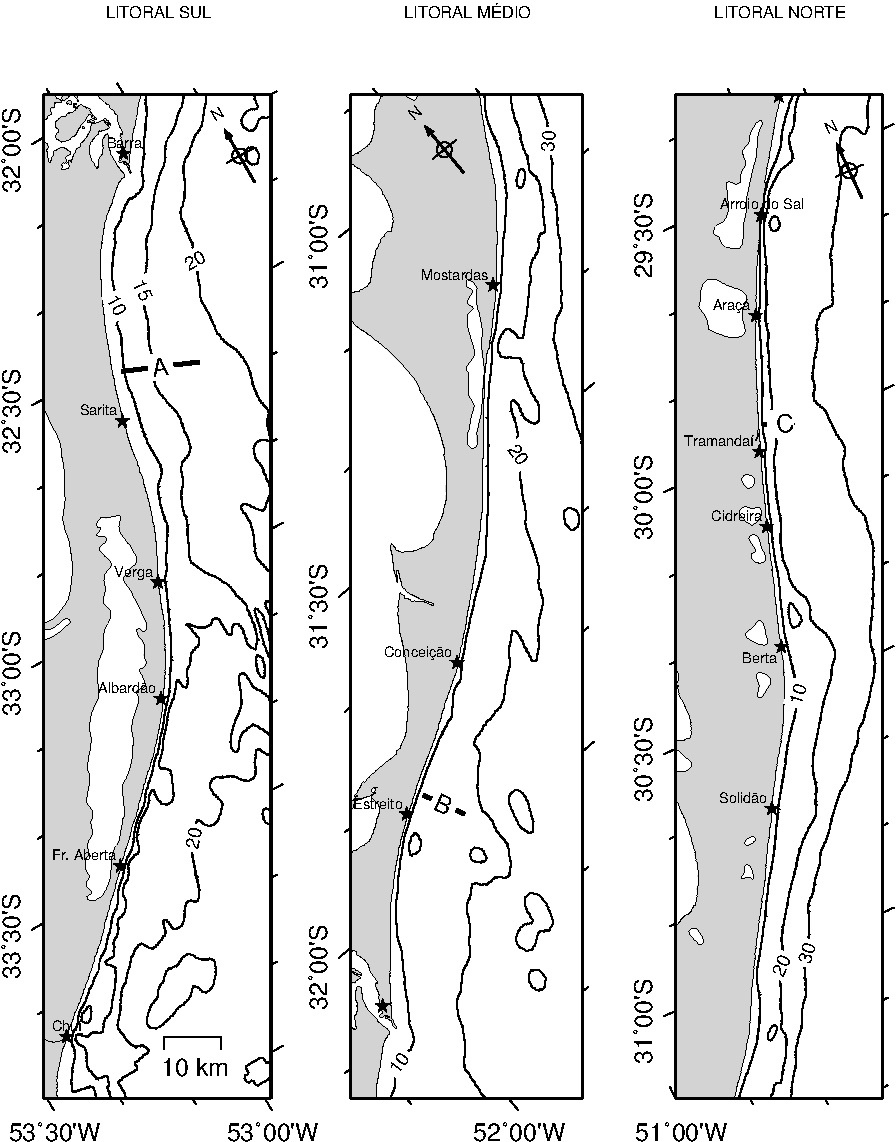
\includegraphics[width=\textwidth]{BATIMETRIA_MAPA}
\end{center}
\caption[Mapas oblíquos das três subáreas, contendo as isóbatas de 10, 15, 20 e 30~m]
	{Mapas oblíquos das três subáreas, contendo as isóbatas de 10, 15 e 20~m para 
         a subárea Litoral Sul, e as de 10, 20 e 30~m para as subáreas Litoral Médio e Norte. 
         As estrelas indicam faróis, e as linhas são os trechos cujos dados foram utilizados na 
         geração de perfis batimétricos (A,B,C).}
\label{fig:batimetria-fig1}
\end{figure}

%%%

Para fins de apresentação a área de estudo foi dividida em três subáreas de mesma extensão, 
as quais receberam a seguinte denominação:

\begin{itemize}

\item Litoral Norte - subárea compreendida entre as latitudes 29°18,6'S e 31°13,2'S;
\item Litoral Médio - subárea compreendida entre as latitudes 30°58,2'S e 32°14,4'S;
\item Litoral Sul - subárea compreendida entre as latitudes 32°01,8'S e 33°51,0'S.

\end{itemize}

Foram escolhidos ainda três trechos, um em cada subárea, onde a coleta de dados acústicos 
ocorreu de forma ortogonal à linha de costa, no intuito de destacar diferenças geomorfológicas 
do fundo marinho entre as subáreas em questão. A partir dos dados adquiridos em cada um desses 
trechos, foram gerados perfis batimétricos (Figura~\ref{fig:batimetria-fig2}).

% FIGURA 2 PERFIS BATIMÉTRICOS
%
%%%%%%%%%%%%%%%%%%%%%%%%%%%%%%%%%%%%%%%%%%%%%%%%%%%%%%%%

\begin{figure}
\begin{center}
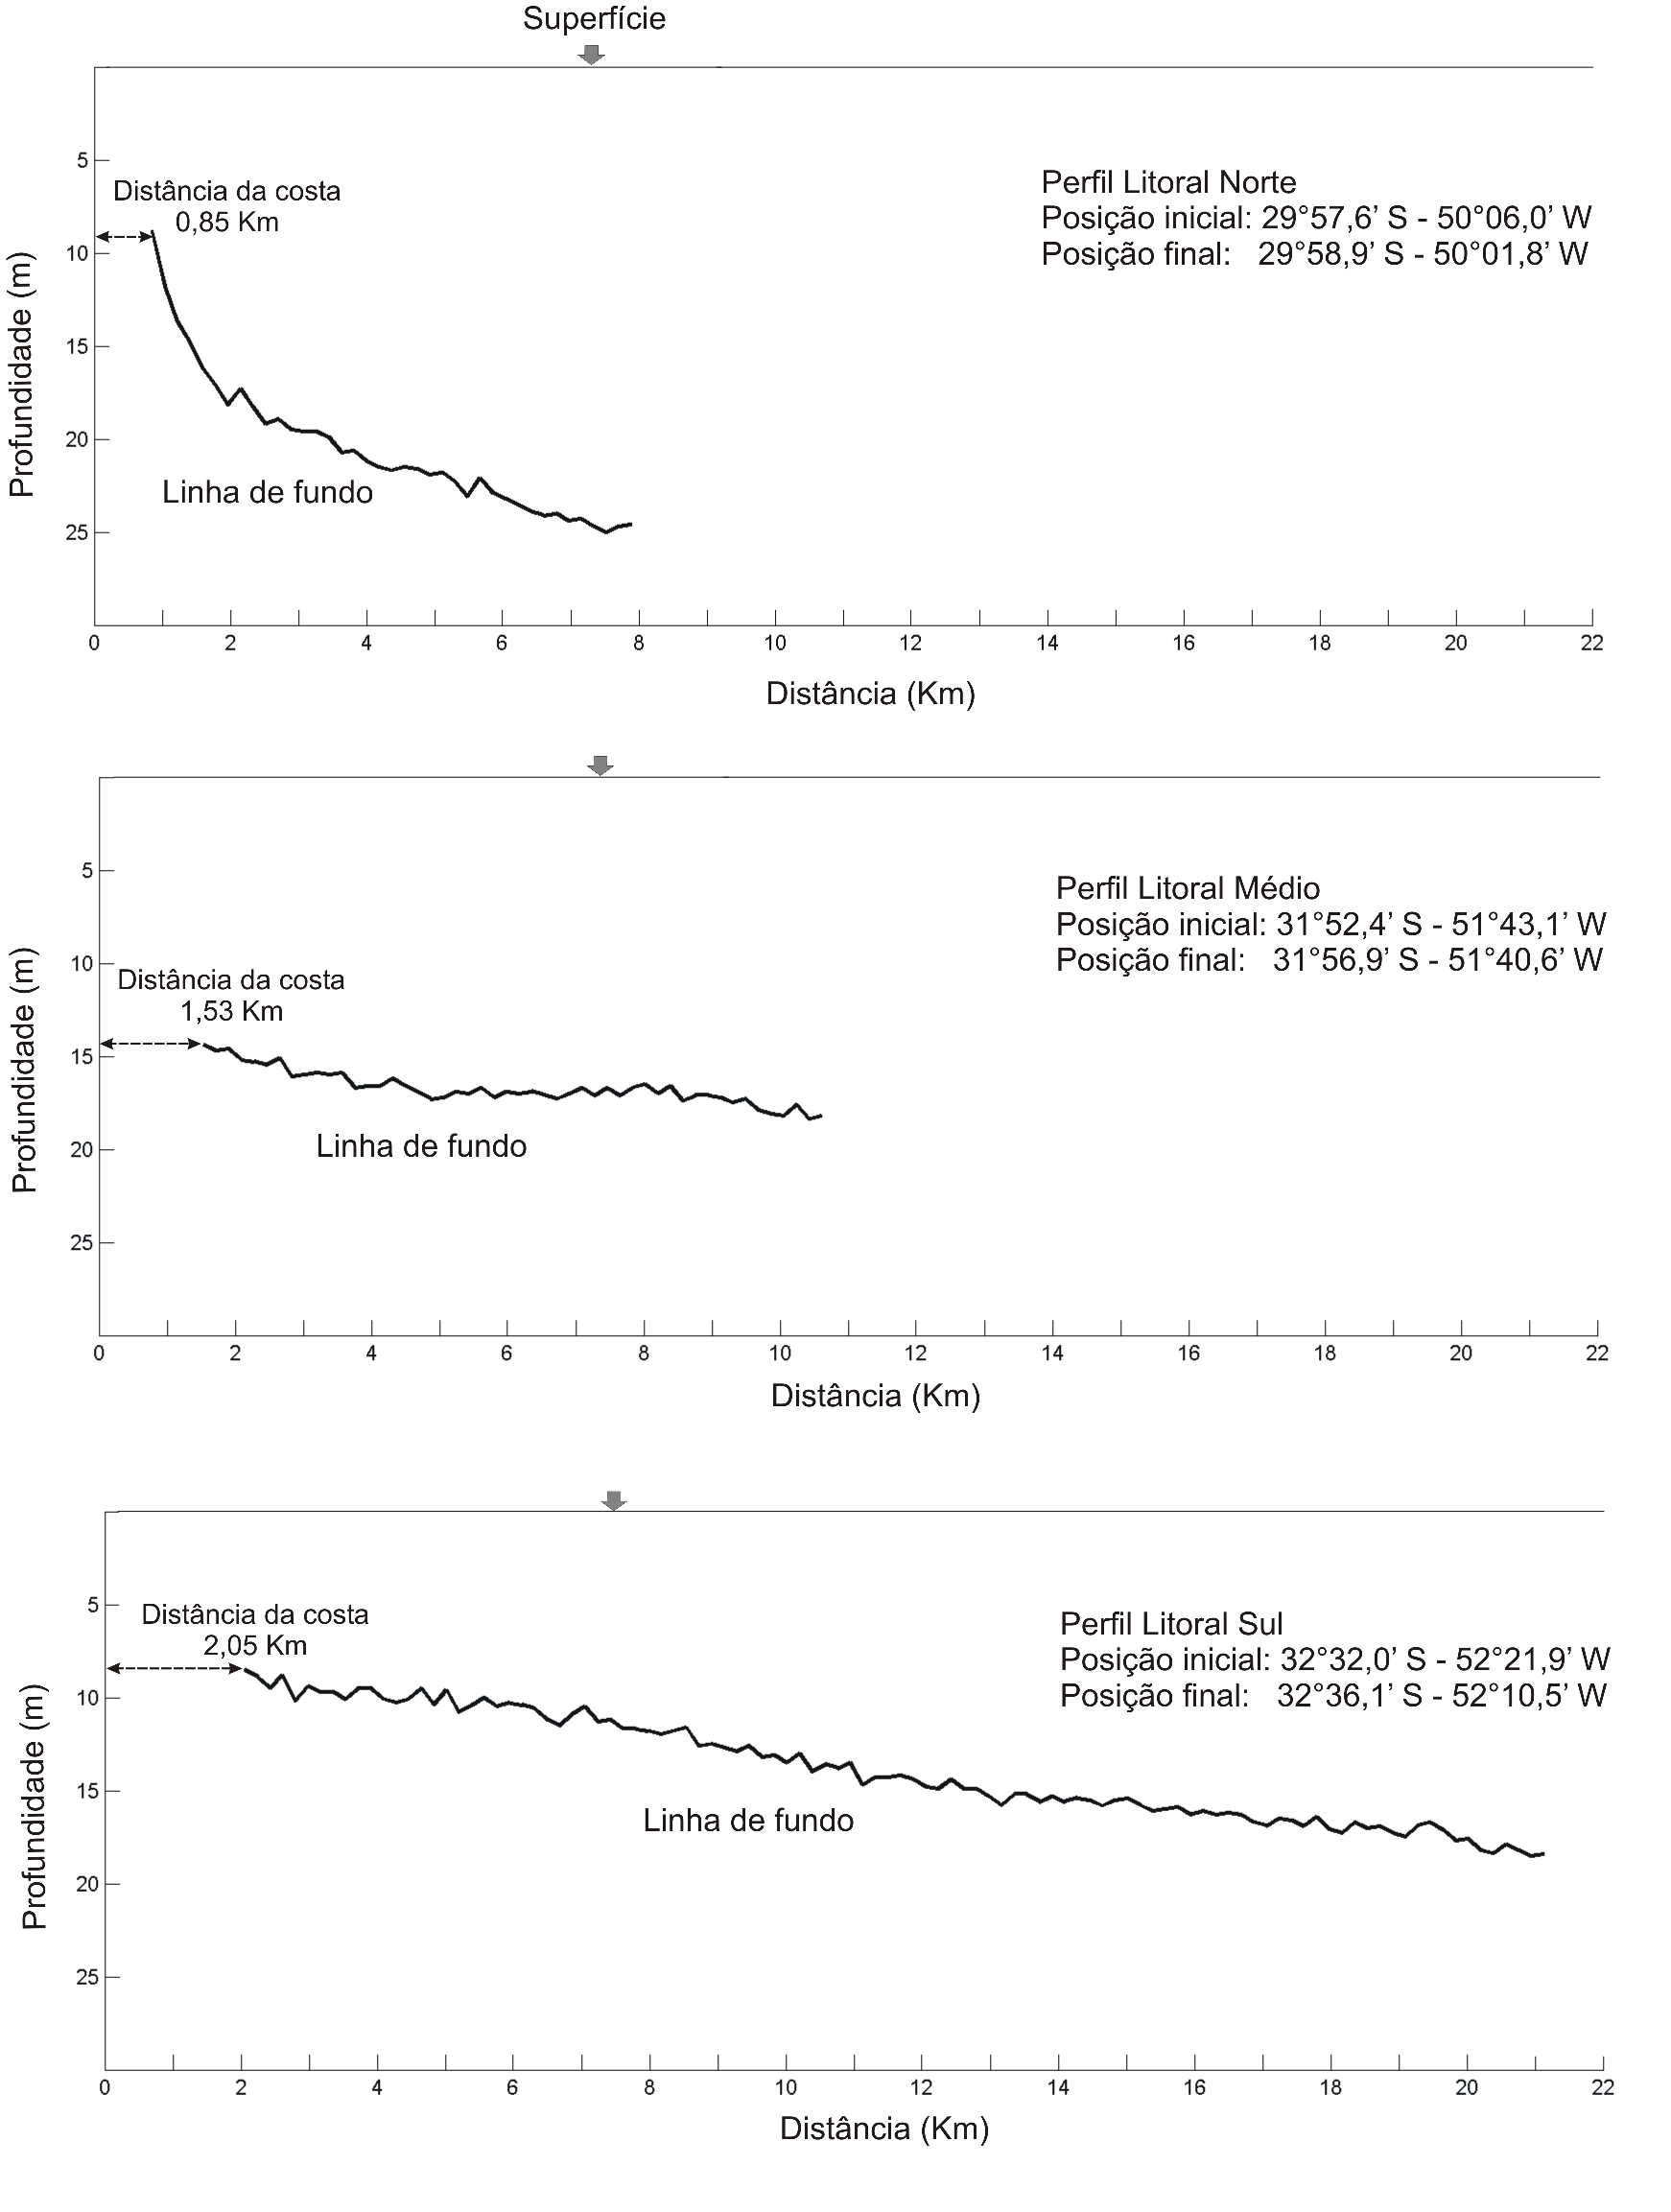
\includegraphics[width=\textwidth]{BATIMETRIA_PERFIS}
\end{center}
\caption[Perfis batimétricos perpendiculares à linha de costa]
	{Perfis batimétricos provenientes de dados acústicos de trechos 
         navegados perpendicularmente à linha de costa, 
         em cada uma das subáreas. Exagero vertical de 733,33~x.}
\label{fig:batimetria-fig2}
\end{figure}

%%%

Uma vez definidas e traçadas as isóbatas de interesse, procedeu-se o cálculo das superfícies, 
por subáreas e por estratos batimétricos. Os resultados desse cálculo são apresentados na 
tabela~\ref{tab:batimetria-tab1}.

%
% TABELA 1 ÁREAS POR FAIXA BATIMÉTRICA
%
%%%%%%%%%%%%%%%%%%%%%%%%%%%%%%%%%%%%%%%%%%%%%%%%%%%

\begin{table}
\caption[Superfícies, por subárea e estratos batimétricos da plataforma 
         do Rio Grande do Sul até a isóbata de 30~m]
        {Superfícies, por subárea, por estratos batimétricos, e somatório das superfícies 
         representando a superfície total da plataforma do Rio Grande do Sul, entre a linha 
         de costa e a isóbata de 30~m.}
\label{tab:batimetria-tab1}	 
\begin{center}
\begin{tabular*}{\textwidth}{c@{\extracolsep{\fill}}cccc}
\toprule
				& 	\multicolumn{4}{c}{Subáreas / superfícies (km\textsuperscript{2})}		\\
\cmidrule(l){2-5}
Faixa batimétrica (m)		& Litoral Norte		& Litoral Médio		& Litoral Sul		& Total		\\
\midrule
0--10				& 381,10		& 419,40		& 828,47		& 1.628,97	\\
11--15				& 332,54		& 816,51		& 2.292,40		& 3.441,45	\\
16--20				& 884,53		& 2.107,12		& 3.110,72		& 6.102,37	\\
21--30				& 2.775,76		& 1.712,68		& 1.688,23		& 6.176,67	\\
\midrule
Total (0--30)			& 4.373,93		& 5.055,71		& 7.919,82		& 17.349,46	\\
\bottomrule
\end{tabular*}
\end{center}
\end{table}

%%%

Observa-se na figura~\ref{fig:batimetria-fig1} o afastamento da isóbata de 10~m em relação à linha de costa, 
que ocorre entre o Farol de Verga e a região localizada entre os Faróis da Barra e do Estreito, 
onde a mesma volta a posicionar-se relativamente próximo à linha de costa. Destacam-se as menores 
profundidades registradas no Litoral Sul, em relação ao Litoral Médio, acentuando-se ainda mais 
no Litoral Norte, se considerarmos pontos localizados a uma mesma distância da linha de costa (Figura~\ref{fig:batimetria-fig2}).
No Litoral Norte, entre os Faróis da Berta e Cidreira, a isóbata de 20~m aproxima-se da linha de costa, 
indicando uma acentuada pendente do leito marinho, se comparado com as demais subáreas, mantendo-se 
este padrão até o extremo norte da região de estudo.

De maneira geral, a pendente do leito marinho diminui de Norte para Sul, o que é evidenciado na figura~\ref{fig:batimetria-fig2},
comparando-se os perfis batimétricos do Litoral Norte com os do Litoral Médio e Sul.

Os valores estimados de superfície por estratos batimétricos (Tabela~\ref{tab:batimetria-tab1}) 
reforçam a idéia de que a subárea Litoral Sul apresenta mais porções rasas 
em relação ao Litoral Médio e este, por sua vez, em relação ao Litoral Norte. 
Considerando-se a superfície total entre a linha de costa e a isóbata de 30~m, 
para a costa do Rio Grande do Sul, verifica-se que 45,6\% dessa superfície 
encontram-se na subárea Litoral Sul, enquanto 29,1 e 25,2\% estão nas subáreas 
Litoral Médio e Norte, respectivamente.

\section*{Condições Oceanográficas}


\subsection*{Campos termohalinos de superfície e fundo}

Em geral, as isotermas de superfície e de fundo estiveram paralelas à costa.
Maiores temperaturas ocorreram nas menores profundidades, mais próximas da costa.
No entanto, observou-se nas isotermas de fundo a intrusão de águas mais frias em menores profundidades
na latitude do Farol de Mostardas (31°15'S), oriundas da região além da isóbata 
de 30~m de profundidade, provavelmente como resultado de fenômenos de ressurgência
na plataforma externa (Figura~\ref{fig:temperatura-sup-e-fundo}).

Os valores de salinidade de superfície e de fundo aumentaram
do sul para o norte. Salinidades maiores que 35~ups foram encontradas 
somente ao norte de Rio Grande (32°10'S).
As isolinhas de salinidade foram oblíquas até
o Farol de Mostardas e paralelas ao norte do mesmo (Figura~\ref{fig:salinidade-sup-e-fundo}). 

Os baixos valores de salinidade encontrados ao sul, e a conformação
das isolinhas de salinidade sugerem
a intrusão de águas de origem continental no sul da região. Enquanto 
a influência das massas de água de origem tropical foi maior ao norte.

% FIGURA TEMPERATURA DE SUP E FUNDO
%
%%%%%%%%%%%%%%%%%%%%%%%%%%%%%%%%%%%%%%%%%%%%%%%%%%%%%%%%

\begin{figure}
\begin{center}
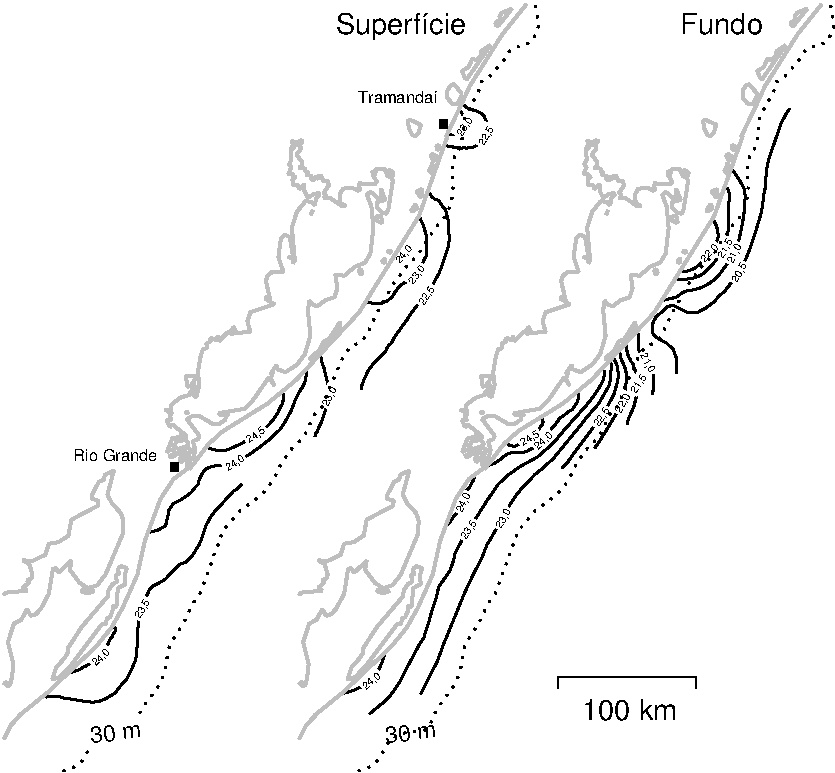
\includegraphics[height=0.6\textheight]{MAPA_TEMPERATURA}
\end{center}
\caption[Isolinhas de temperatura da superfície e fundo]
	{Isolinhas de temperatura da superfície e fundo (°C) nas águas rasas da
         plataforma do Rio Grande do Sul no verão de 2005.}
\label{fig:temperatura-sup-e-fundo}
\end{figure}

%%%


% FIGURA SALINIDADE DE SUP E FUNDO
%
%%%%%%%%%%%%%%%%%%%%%%%%%%%%%%%%%%%%%%%%%%%%%%%%%%%%%%%%

\begin{figure}
\begin{center}
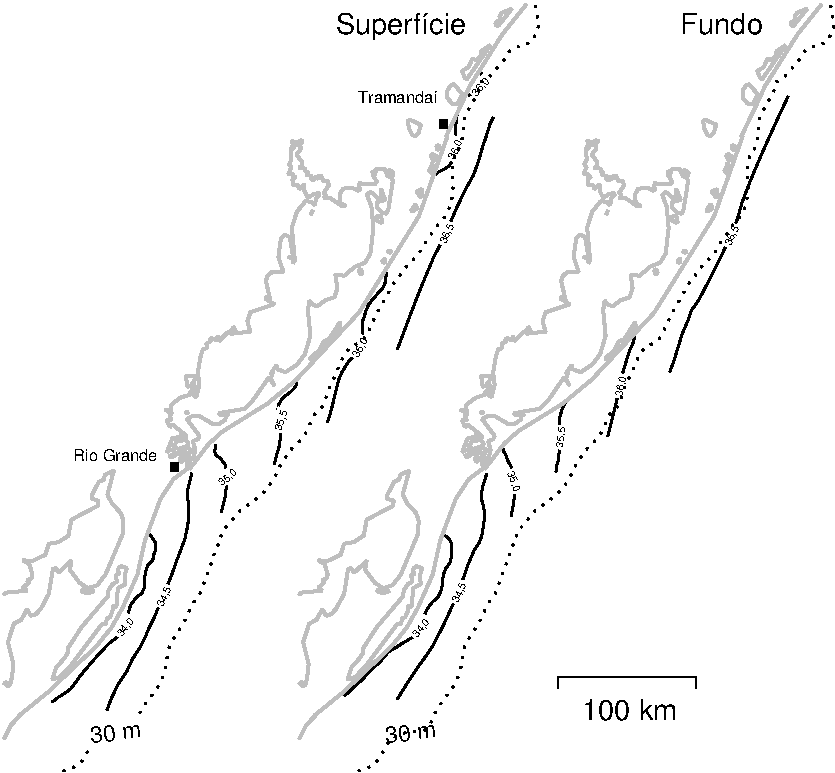
\includegraphics[height=0.6\textheight]{MAPA_SALINIDADE}
\end{center}
\caption[Isolinhas de salinidade da superfície e fundo]
	{Isolinhas de salinidade da superfície e fundo (UPS) nas águas rasas da
         plataforma do Rio Grande do Sul no verão de 2005.}
\label{fig:salinidade-sup-e-fundo}
\end{figure}

%%%


\subsection*{Massas de água}

% Tabela ?. Massas de água na plataforma continental do sul do brasil. Fonte: Emilsson 1961
% 
% massa de água			sigla		salinidade			temperatura
% água tropical			TW			> 36 ups			> 20 C
% água sub-antartica	SAW			33,7-34,15 ups		4-15 C
% água subtropical		STW			34,2-36,0 ups		20-20 C

O diagrama T-S das estações oceanográficas evidenciou a existência de duas
massas de água na região costeira da Plataforma Sul. A Água Tropical (AT)
caracterizada por temperaturas acima de 20°C e salinidades acima de 36~ups, e
a Água Costeira (AC), de elevadas temperaturas e baixa salinidade,
e com valores de sigma-0 inferiores a 24,5~kg/m\textsuperscript{3}.
A AT estava presente na região costeira entre Torres (29°20'S) e Solidão (30°42'S), 
enquanto a AC ocorreu principalmente entre Rio Grande (32°10'S) e o Chuí (34°S).
Na região entre Solidão e Rio Grande, ambas as massas de águas estiveram
presentes, caracterizando uma zona de transição e mistura das massas
de água (Figura~\ref{fig:diagrama-ts}).

% FIGURA DIAGRAMA T-S
%
%%%%%%%%%%%%%%%%%%%%%%%%%%%%%%%%%%%%%%%%%%%%%%%%%%%%%%%%

\begin{figure}
\begin{center}
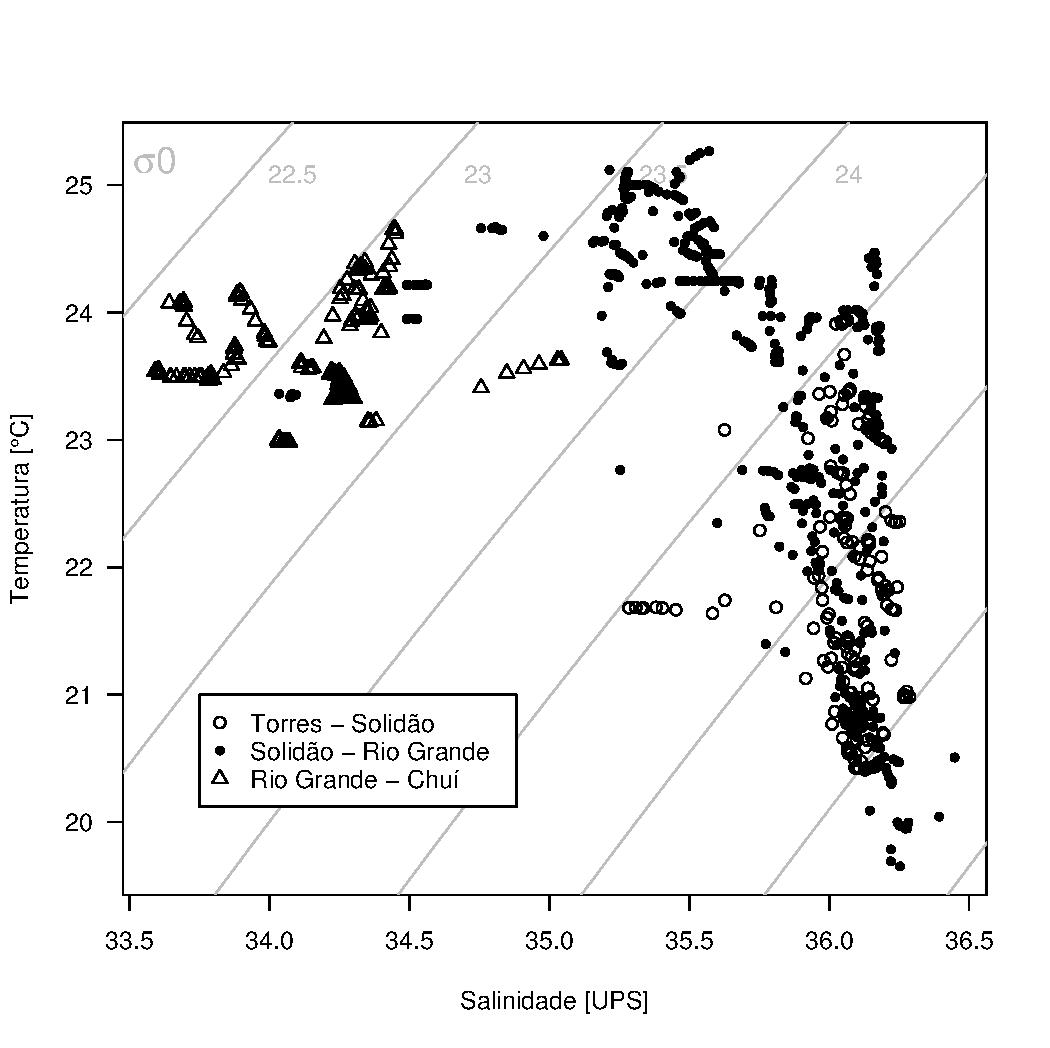
\includegraphics[width=\textwidth]{DIAGRAMATS}
\end{center}
\caption[Diagrama de temperatura versus salinidade das águas rasas da plataforma do Rio Grande do Sul no verão]
	{Diagrama de temperatura versus salinidade das águas rasas da plataforma do Rio Grande do Sul no verão.}
\label{fig:diagrama-ts}
\end{figure}

%%%

%%%%%%%%%%%%%%%%%%%%%%%%%%%%%%%%%%%%%%%%%%%%%%%%%%%%%%%%%%%%%%%%%

\chapter[Biologia e status de conservação da viola  \emph{Rhinobatos horkelii}]
        {Biologia e status de conservação da viola  \emph{Rhinobatos horkelii}}\label{chap:viola}


\chapterprecishere{Carolus Maria Vooren \\
                   Rosângela Paula Lessa \\
                   Sandro Klippel}

\chapterprecistoc{\small C. M. Vooren, R. P. Lessa e S. Klippel}

\makeevenhead{myheadings}{Vooren, C. M., Lessa, R. P. e S. Klippel}{}{}
% \makeoddhead{myheadings}{}{}{Biologia e status de conservação da viola  \emph{Rhinobatos horkelii}}
\makeoddhead{myheadings}{}{}{Biologia e status de conservação da viola}

\newpage

\section*{Sistemática,  morfologia e evolução}

A viola (Figura~\ref{fig:violas-noarrasto}) é uma raia e pertence à família Rhinobatidae.
Na costa Atlântica das Américas, essa família é representada pelos 
gêneros \emph{Rhinobatos} e \emph{Zapteryx}. A morfologia do gênero \emph{Rhinobatos} é caracterizada 
pela cauda longa e  larga, pela envergadura relativamente pequena das nadadeiras 
peitorais, pelo focinho rígido e proeminente,  e pelo corpo inteiramente coberto 
com dentículos dérmicos. \emph{Zapteryx} tem morfologia semelhante, exceto o focinho que 
é curto e arredondado. Na costa do Brasil o gênero \emph{Zapteryx} é representado por  
\emph{Z. brevirostris} (Müller \& Henle 1841), e o gênero \emph{Rhinobatos} por 
\emph{R. horkelii} Müller \& Henle 1841 e \emph{R. percellens} Walbaum 1792 \citep{menni2000}. % (Menni e Stehmann, 2000).  
No Brasil as espécies de \emph{Rhinobatos} são conhecidas como ``viola'' ou ``raia-viola'', 
enquanto \emph{Z. brevirostris} é denominado de ``banjo'' \citep{FIGUEIREDO1977}. % (Figueiredo, 1977; Vooren et al., 2003). 

%
% FOTOGRAFIA DE VIOLAS CAPTURADAS NO ARRASTO DE FUNDO
%
%%%%%%%%%%%%%%%%%%%%%%%%%%%%%%%%%%%%%%%%%%%%%%%%%%%%%%%%

\begin{figure}
\begin{center}
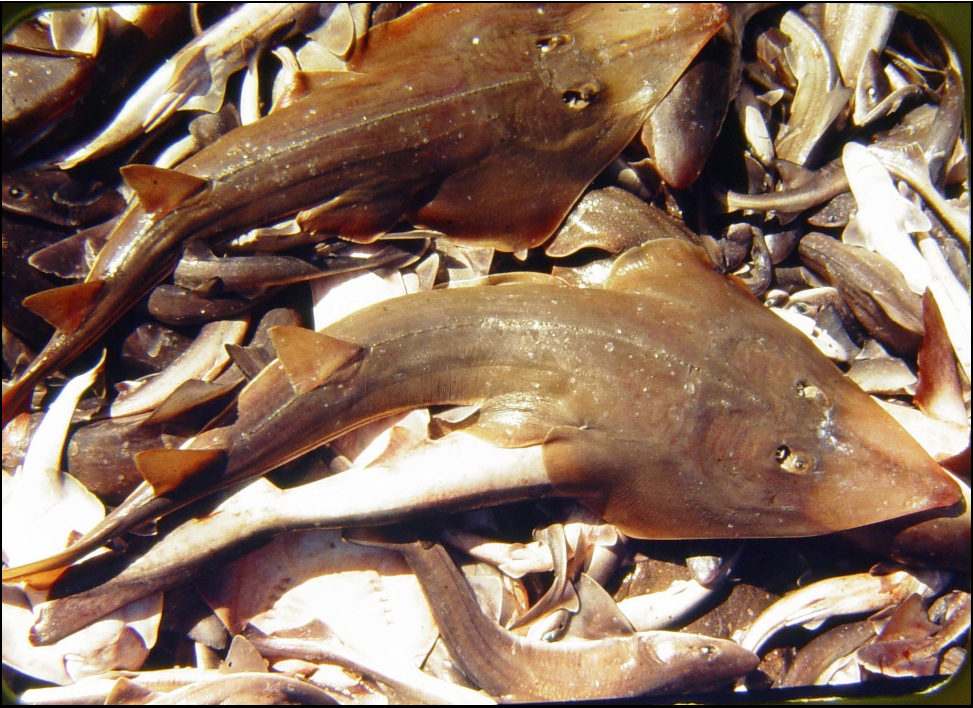
\includegraphics[width=\textwidth]{VIOLAS_NOARRASTO}
\end{center}
\caption[Duas violas \emph{Rhinobatos horkelii} em uma captura com rede de arrasto de fundo 
         na plataforma do Rio Grande do Sul no ano de 1980.]
	{Duas violas \emph{Rhinobatos horkelii} em uma captura com rede de arrasto de fundo 
         na plataforma do Rio Grande do Sul no ano de 1980. 
	 A rede de arrasto captura a viola junto com muitas outras espécies de peixes.}
\label{fig:violas-noarrasto}
\end{figure}

%%%

Segundo \citet[p. 56--71, tradução pelos autores]{bigelow1953} % Bigelow e Schroeder (1953, p. 56-71, tradução pelos autores), 
\emph{Rhinobatos horkelii} é ``\ldots o maior \emph{Rhinobatos} do lado oeste do Atlântico'', 
isto porque um macho de 70~cm de CT era nitidamente imaturo, e a cor da pele 
no lado dorsal do corpo de \emph{R. horkelii} é ``\ldots uniformemente verde-oliva acinzentado 
ou marrom-chocolate, sem marcas claras ou escuras''. Segundo esses mesmos autores, 
\emph{R. percellens} é uma espécie de pequeno porte, pois um macho de 56~cm de CT 
era sexualmente maduro, e o CT máximo da espécie é de cerca de 95~cm. A cor da 
pele no lado dorsal do corpo de \emph{R. percellens} é marrom com ``\ldots os flancos geralmente 
com pintas ou manchas mais escuras, vagamente delineadas e em número variado, 
freqüentemente formando-se bandas transversais sobre a cauda  \ldots a maioria dos 
espécimes possui cerca de 40 a 45 pintas esbranquiçadas em ambos os lados da 
linha mediana dorsal, de tamanho semelhante à pupila do olho, dispostas 
irregularmente porém simetricamente sobre os dois lados do tronco''.   

Os 9.754 indivíduos de \emph{Rhinobatos} da Plataforma Sul examinados por \citet{lessa1982} % Lessa (1982) 
foram \emph{R. horkelii} com base no tamanho corporal (Tabela~\ref{tab:parametros-populacionais-viola})
e da cor da pele. Pelos mesmos critérios, os 23 indivíduos de \emph{Rhinobatos} 
capturados no Cruzeiro SALVAR em fevereiro de 2005 nas águas costeiras 
entre Torres e Albardão foram \emph{R. horkelii}. \citet{sadowsky1973} % Sadowsky (1973) 
identificou  como \emph{R. horkelii} os 99 espécimes de \emph{Rhinobatos} coletados na Plataforma Sul 
no ano de 1972. Registros da ocorrência de \emph{R. percellens} na Plataforma Sul \citep{chao1982} % (Chão et al., 1982) 
decorrem provavelmente de problemas com um dos critérios 
publicados para a identificação de \emph{R. horkelii} e \emph{R. percellens}. Com base na 
medição de apenas dois espécimes de ambas estas espécies, com CT de 50 a 59~cm e 
coletados na costa do Rio de Janeiro,  \citet{bigelow1953} % Bigelow e Schroeder (1953) 
apresentam o tamanho relativo da fossa nasal como critério para distinguir entre \emph{R. horkelii} 
e \emph{R. percellens} (Figura~\ref{fig:viola-vistaventral}). % FIGURA 2
Esse critério nem sempre permite a identificação de espécimes de 
todos os tamanhos e em todas as áreas onde essas espécies ocorrem, como é demonstrado 
pelo fato de que duas fêmeas de \emph{R. horkelii} com CT de 115 e 131~cm, coletados no 
Cruzeiro SALVAR, têm o tamanho da fossa nasal intermediário entre os valores  
que \citet{bigelow1953} % Bigelow e Schroeder (1953) 
apresentam para \emph{R. horkelii} e \emph{R. percellens}. 
Com os critérios do tamanho corporal e da cor da pele, a viola da Plataforma Sul 
é \emph{R. horkelii} e portanto, as estatísticas da pesca da viola na Plataforma Sul 
referem-se a essa espécie. Essa conclusão é corroborada pelo fato de que no 
monitoramento dos desembarques no porto de Itajaí nos anos de 1994 a 1999,  
\emph{R. horkelli} foi classificado como ``abundante'', e \emph{R. percellens} 
como ``espécie rara'' \citep{mazzoleni1999}. % (Mazzoleni e Schwingel, 1999). 
A frota de arrasto de fundo de Itajaí opera na plataforma entre Rio de Janeiro e Chuí, 
mas suas capturas de viola provêm principalmente da Plataforma Sul \citep{martins2003}. % (Martins e Schwingel, 2003).  

%
% Figura 2. Vista ventral da cabeça da viola Rhinobatos horkelii do sul do Brasil. 
% De cima para baixo: as duas fossas nasais onde se situa o olfato; a boca com as 
% camadas de dentes pequenos e achatados; os cinco pares de fendas branquiais. 
%
%%%%%%%%%%%%%%%%%%%%%%%%%%%%%%%%%%%%%%%%%%%%%%%%%%%%%%%%

\begin{figure}
\begin{center}
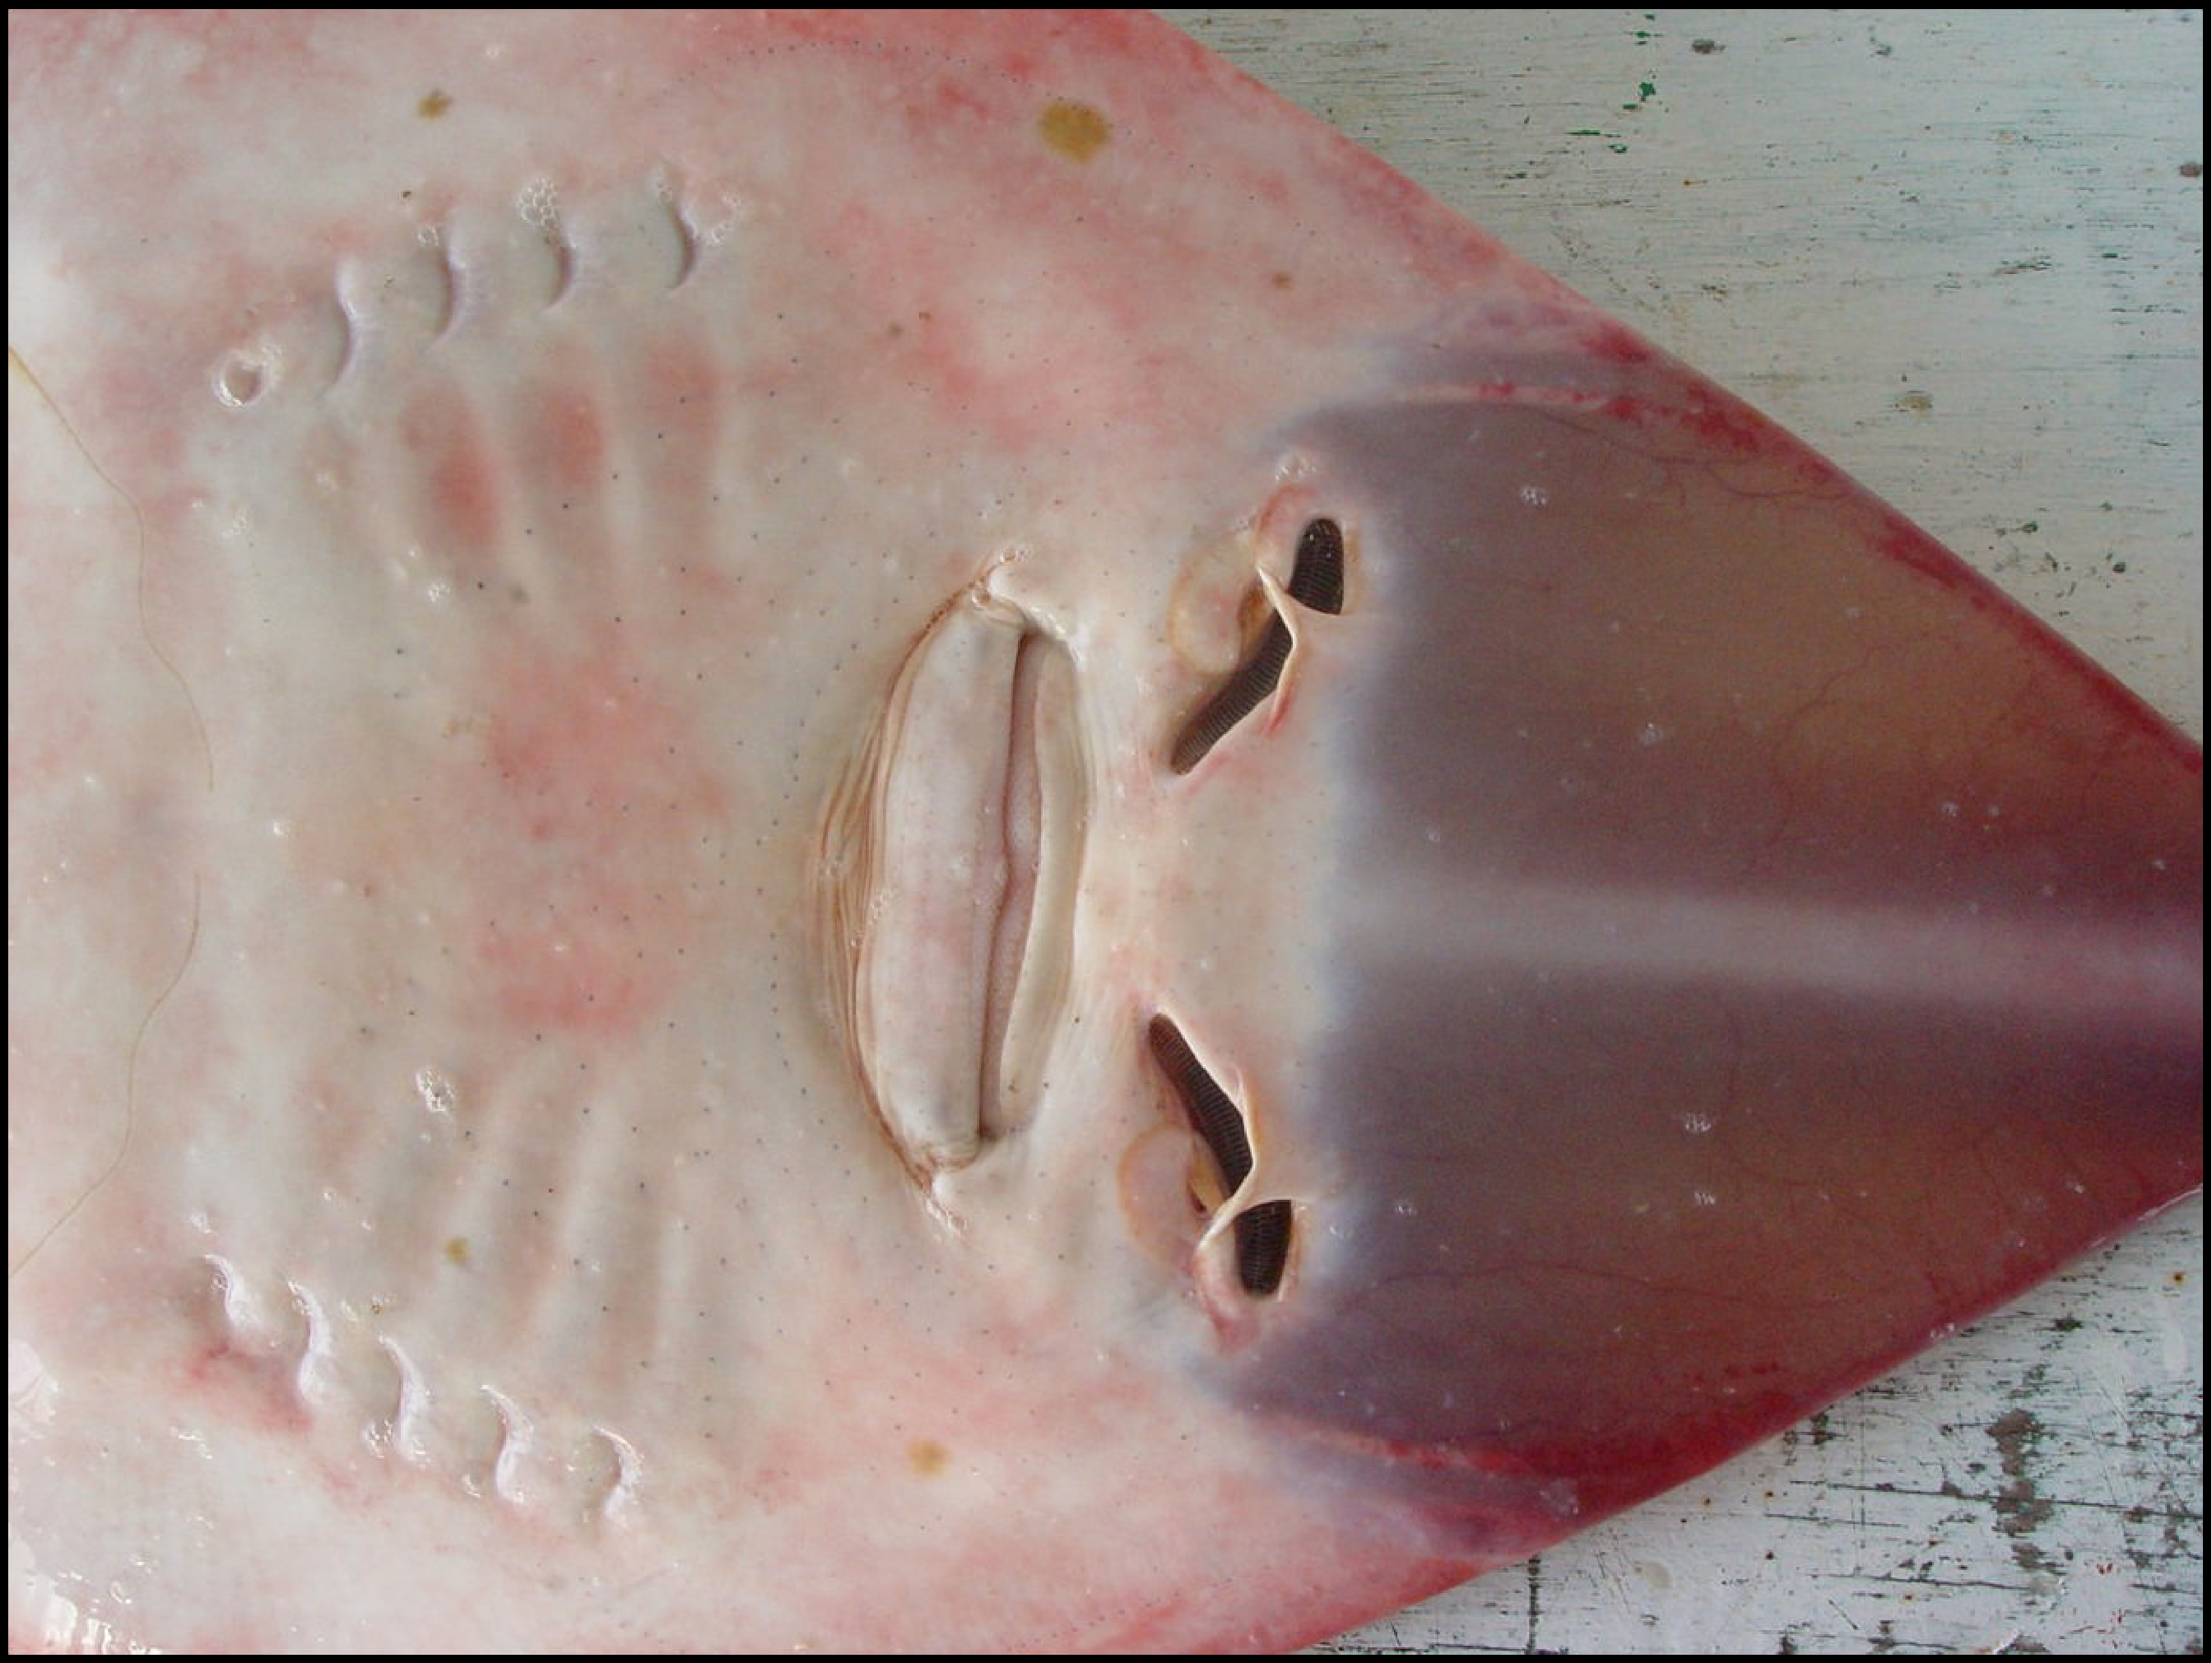
\includegraphics[width=\textwidth]{VIOLA_VISTA_VENTRAL}
\end{center}
\caption[Vista ventral da cabeça da viola \emph{Rhinobatos horkelii} do sul do Brasil]
	{Vista ventral da cabeça da viola \emph{Rhinobatos horkelii} do sul do Brasil. 
         Da direita para a esquerda: o focinho; as duas fossas nasais onde se situa o olfato; a boca com as 
         camadas de dentes pequenos e achatados; os cinco pares de fendas branquiais.}
\label{fig:viola-vistaventral}
\end{figure}

%%%%



%
% TABELA PARÂMETROS POPULACIONAIS DA VIOLA
%
%%%%%%%%%%%%%%%%%%%%%%%%%%%%%%%%%%%%%%%%%%%%%%%%%%%

\begin{table}
\caption[Estatísticas populacionais da viola \emph{Rhinobatos horkelii} 
         na Plataforma Sul do Brasil]
        {Estatísticas populacionais da viola \emph{Rhinobatos horkelii} 
         na Plataforma Sul do Brasil segundo \citet{lessa1982}, mas dados 
	 sobre o menor CT e PT ao nascer provêm do Cruzeiro SALVAR em 2005.
	 CT = comprimento total, PT = peso total.}
\label{tab:parametros-populacionais-viola}	 
\begin{center}
\begin{tabularx}{\textwidth}{Xcc}
\toprule
			& Macho		& Fêmea		\\
\midrule
\addlinespace
CT máximo (cm)		& 129		& 135		\\
\addlinespace
Peso eviscerado 
máximo (kg)		& 7,0		& 8,0		\\
\addlinespace
Idade máxima (anos)	& 15		& 28		\\
\addlinespace
CT do menor 
adulto (cm)		& 75		& 91		\\
\addlinespace
CT com 100\% de
maturação 
sexual (cm)		& 87		& 110		\\
\addlinespace
Idade do menor 
adulto (anos)		& 4		& 5		\\
\addlinespace
Idade com 100\% 
maturação 
sexual (anos)		& 5		& 8		\\
\addlinespace
Número de filhotes 
por gestação		& \multicolumn{2}{c}{3--12, média 6}	\\
\addlinespace
CT ao nascer (cm) 	& \multicolumn{2}{c}{22--29}	\\
\addlinespace
PT ao nascer (g)	& \multicolumn{2}{c}{35--67}	\\
\addlinespace
Parâmetros da curva 
de crescimento de von 
Bertalanffy: 		&	\\
\addlinespace
L$\infty$ (cm)		& \multicolumn{2}{c}{135,51}	\\
\addlinespace
K			& \multicolumn{2}{c}{0,194}	\\
\addlinespace
t$_0$ (anos)		& \multicolumn{2}{c}{-1,0785}	\\
\bottomrule
\end{tabularx}
\end{center}
\end{table}

%%%

Nos desembarques da pesca comercial no Rio Grande do Sul, as carcaças de \emph{R. horkelii}  
são o corpo eviscerado com ou sem a cabeça ou o focinho, mas sempre com as nadadeiras 
peitorais, as nadadeiras pélvicas e a cauda.  Carcaças de \emph{Zapteryx brevirostris} têm 
geralmente essa mesma conformação, mas ocasionalmente são desembarcadas somente as 
caudas dessa espécie. A carcaça de \emph{R. horkelii}  tem a largura do disco de cerca de duas 
vezes a largura do corpo entre as bases posteriores das nadadeiras peitorais e três vezes 
a largura da cauda  entre as bases posteriores das nadadeiras pélvicas, e possui entre 
a cabeça e a 1ª nadadeira dorsal uma fileira de pequenos espinhos ou tubérculos. 
A carcaça de \emph{Z. brevirostris} tem a largura do disco de cerca de três vezes a largura 
do corpo entre as bases posteriores das nadadeiras peitorais e cinco vezes a largura da 
cauda  entre as bases posteriores das nadadeiras pélvicas, e possui entre a cabeça 
e a 1ª nadadeira dorsal  uma fileira de 20 a 25 proeminências cônicas com um tubérculo 
no ápice de cada uma. Essa última característica, em combinação com a cor da pele e 
a cobertura de toda a pele com dentículos dérmicos, permite a identificação de 
caudas desta espécie  \citep{vooren2003}. % (Vooren et al., 2003).  % <- referência ao guia de carcaças

Entre os Batoidea atualmente existentes, a família Rhinobatidae é o único táxon com 
registros fósseis do período Jurássico (Figura~\ref{fig:fossil-viola}). 
Das demais famílias de raias existentes, os registros fósseis mais antigos são do 
período Cretáceo. Dos elasmobrânquios atualmente existentes, apenas seis famílias 
tiveram sua origem antes do período Cretáceo \citep{cappetta1987}. % (Cappetta, 1987). 
\emph{R. horkelii} é representante da família mais antiga das raias atuais e pertence, entre 
os elasmobrânquios atuais, a uma das poucas famílias com idade paleontológica 
de mais de 120 milhões de anos \citep{cappetta1987}. Isto é um dos motivos para a
conservação da viola.

%
% FÓSSIL DE VIOLA
%
%%%%%%%%%%%%%%%%%%%%

\begin{figure}
\begin{center}
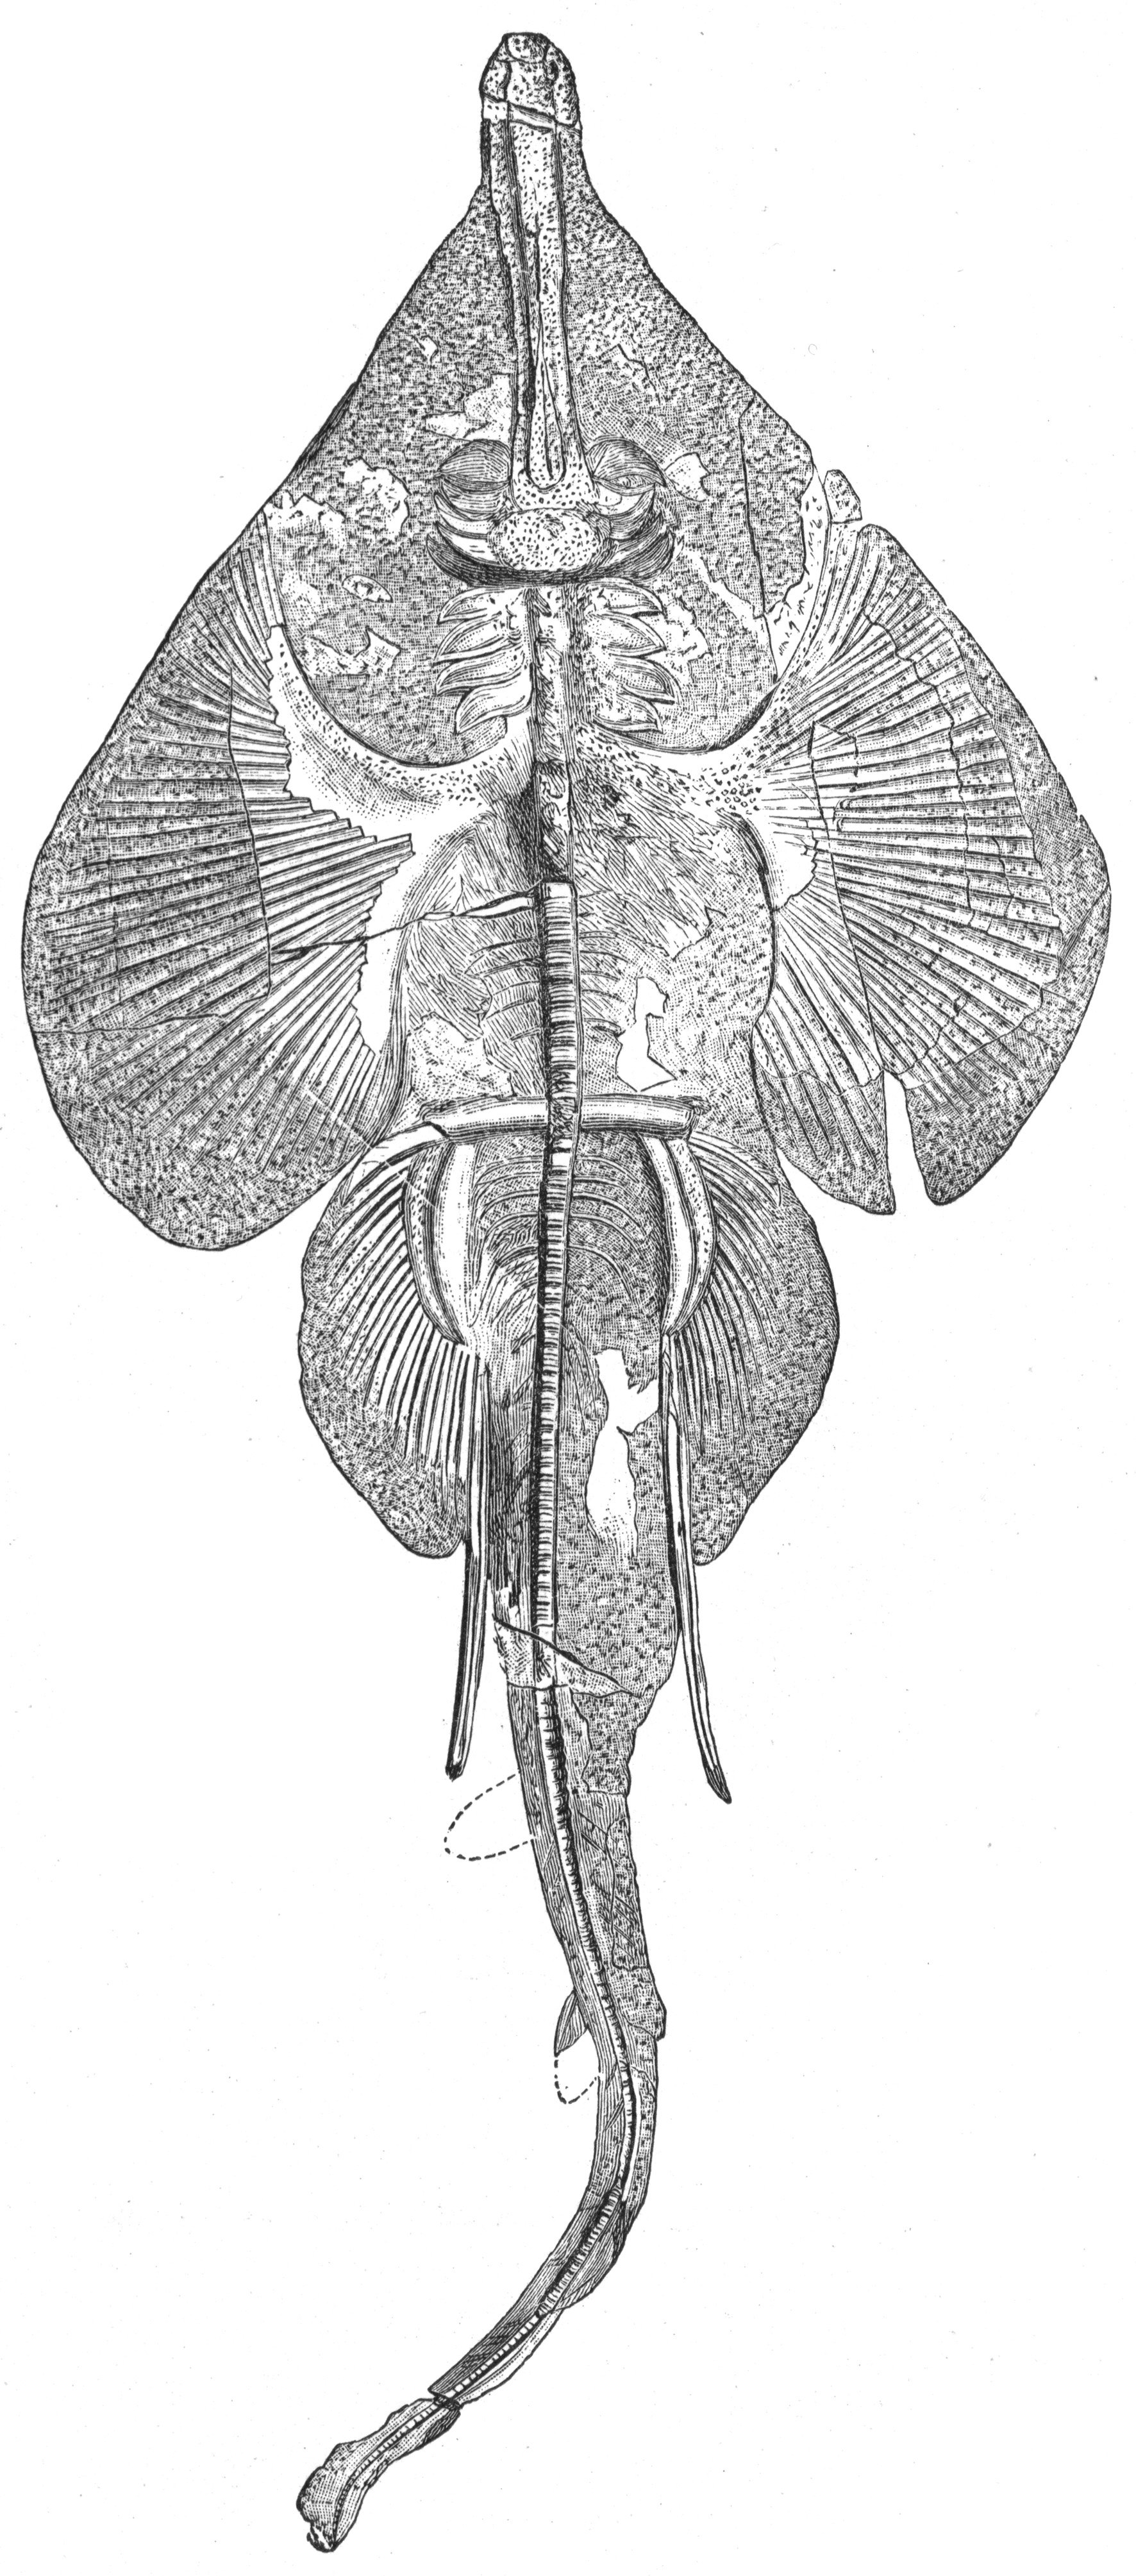
\includegraphics[height=0.8\textheight]{VIOLA_FOSSIL}
\end{center}
\caption[Fóssil de um macho adulto de \emph{Rhinobatos bugesiacus}]
	{Um fóssil de um macho adulto de \emph{Rhinobatos bugesiacus}, 
	 de 160~cm de comprimento, encontrado em uma camada do Jurássico 
	 Superior na localidade de Eichstatt, Alemanha, segundo \citet{abel1924}.} % Abel (1924).  }
\label{fig:fossil-viola}
\end{figure}

%%%

\section*{Distribuição geográfica}

Na costa do Brasil, \emph{R. percellens} ocorre desde Amapá (lat. 4°N) até Paraná (lat. 25°S). 
A distribuição mundial de \emph{R. horkelii} estende-se desde São Paulo (lat. 23°S) até a 
Província de Buenos Aires (lat. 39°S) \citep{menni2000}. % (Menni e Stehmann, 2000). 
\emph{R. horkelii} é importante recurso pesqueiro somente na Plataforma Sul do Brasil, 
onde nos anos de 1975 a 1987 as capturas anuais da espécie foram 
de 636 a 1.803 t \citep{miranda2003}. % (Miranda e Vooren, 2003). 
Na Argentina a espécie é capturada como fauna acompanhante na pesca de camarões \citep{menni2000}. % (Menni e Stehmann, 2000). 
Ao longo da costa oceânica do Uruguai, \emph{R. horkelii} ocorre com baixa densidade e faz parte 
da captura da pescaria mista com o arrasto de fundo na plataforma interna, com capturas 
anuais de cerca de 3~t nos anos de 2000 e 2001 \citep{meneses1999,paesch2003}. % (Meneses, 1999; Paesch e Domingo, 2003). 
Dentro da distribuição geográfica de \emph{R. horkelii}, a Plataforma Sul do Brasil é a única 
área com elevada abundância dessa espécie.

Nos levantamentos pretéritos com arrasto de fundo entre as latitudes de 28°00'S e 34°30'S, 
\emph{R. horkelii} foi comum em toda a plataforma ao sul da latitude de 29°40'S (Figura~\ref{fig:mapa-viola-ocorrencias}).
No Cruzeiro SALVAR, \emph{R. horkelii} ocorreu desde a latitude de 33°00'S frente a Albardão 
até a latitude de 29°24'S em frente à Torres, que foi o limite norte da área do cruzeiro. 
\citet{martins2003} informam que na plataforma externa entre a latitude de 28°40'S 
do Cabo de Santa Marta Grande e a latitude de 30°00'S em frente de Tramandaí, 
a frota de arrasto simples de Itajaí obteve importantes 
capturas de \emph{R. horkelii} em 2000--2002. A distribuição contínua de \emph{R. horkelii} 
sobre a Plataforma Sul, e o fato de que importantes pescarias dessa espécie existem somente na Plataforma Sul, 
são evidências de que a viola da Plataforma Sul constitui uma unidade em termos do manejo 
pesqueiro e da conservação da biodiversidade. 

%
% MAPA COM OCORRÊNCIAS DA VIOLA NOS LEVANTAMENTOS PRETÉRITOS
%
%%%%%%%%%%%%%%%%%%%%%%%%%%%%%%%%%%%%%%%%%%%%%%%%%%%%%%%%%%%%%%%%%%%%%%

\begin{figure}
\begin{center}
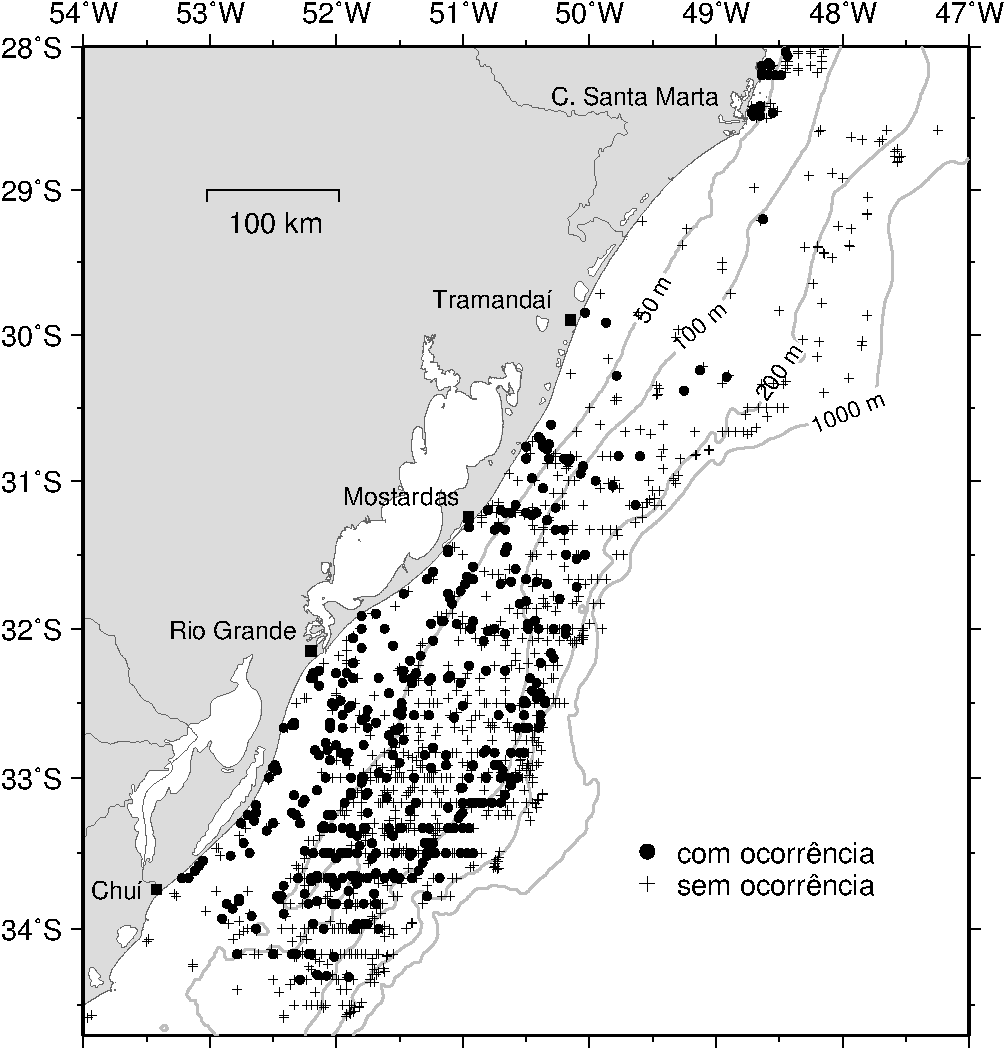
\includegraphics[width=\textwidth]{MAPA_OCORRENCIAS_VIOLA}
\end{center}
\caption[A distribuição das ocorrências da viola \emph{Rhinobatos horkelii} nos levantamentos 
	 pretéritos da Plataforma Sul com arrasto de fundo]
	{A distribuição das ocorrências da viola \emph{Rhinobatos horkelii} nos levantamentos 
	 pretéritos da Plataforma Sul com arrasto de fundo nos anos de 1972--2005.}
\label{fig:mapa-viola-ocorrencias}
\end{figure}

%%%

\section*{Hábitat, alimentação e reprodução}

As espécies de \emph{Rhinobatos} em geral vivem no ambiente bentônico da plataforma 
continental, em fundos de areia ou lama \citep{poll1951,bigelow1953,last1994}. % (Poll,1951; Bigelow e Schroeder, 1953; Last e Stevens, 1994). 
Na Plataforma Sul, \emph{Rhinobatos horkelii} ocorre ao longo do ano, sem variações sazonais da sua 
abundância na área como um todo, sendo classificado como espécie residente \citep{vooren1997}. % (Vooren, 1997). 
Na Argentina a espécie ocorre nas profundidades de 5 a 44~m, em temperaturas 
de 17 a 23°C \citep{menni2000}. % (Boschi e Scelzo, 1967; Gosztonyi,1981; ambos apud  Menni e Stehmann, 2000)

A espécie é vivípara com gestação lecitotrófica \emph{sensu} \citet{wourms1988}, % Wourms et al. (1988), 
o que significa que o embrião se desenvolve com base na matéria orgânica 
presente na forma do vitelo do ovócito maduro (Figura~\ref{fig:foto-embrioes-viola}). % FOTO COM EMBRIÕES DA VIOLA !! EDITAR !!!
Segundo \citet{lessa1982}, esse ovócito contém em média 30~g de vitelo, 
e com isto o embrião se desenvolve até nascer com o peso médio 
de cerca de 50~g (Tabela~\ref{tab:parametros-populacionais-viola}).  
Essa diferença entre os pesos do vitelo e do neonato ocorre porque o 
vitelo contém pouca água, enquanto o embrião absorve água do líquido 
uterino que é produzido pela mãe \citep{ranzi1932}. % (Ranzi, 1932). 
Ao nascer, o neonato ainda possui dentro do seu abdômen uma reserva 
de cerca de 7~g de vitelo que o sustenta durante os primeiros 
dias da sua vida livre \citep{lessa1982}. % (Lessa, 1982). % <- referência da tese da Rosangela !

%
% FOTO COM EMBRIÕES DA VIOLA
%
%%%%%%%%%%%%%%%%%%%%%%%%%%%%%%

\begin{figure}
\begin{center}
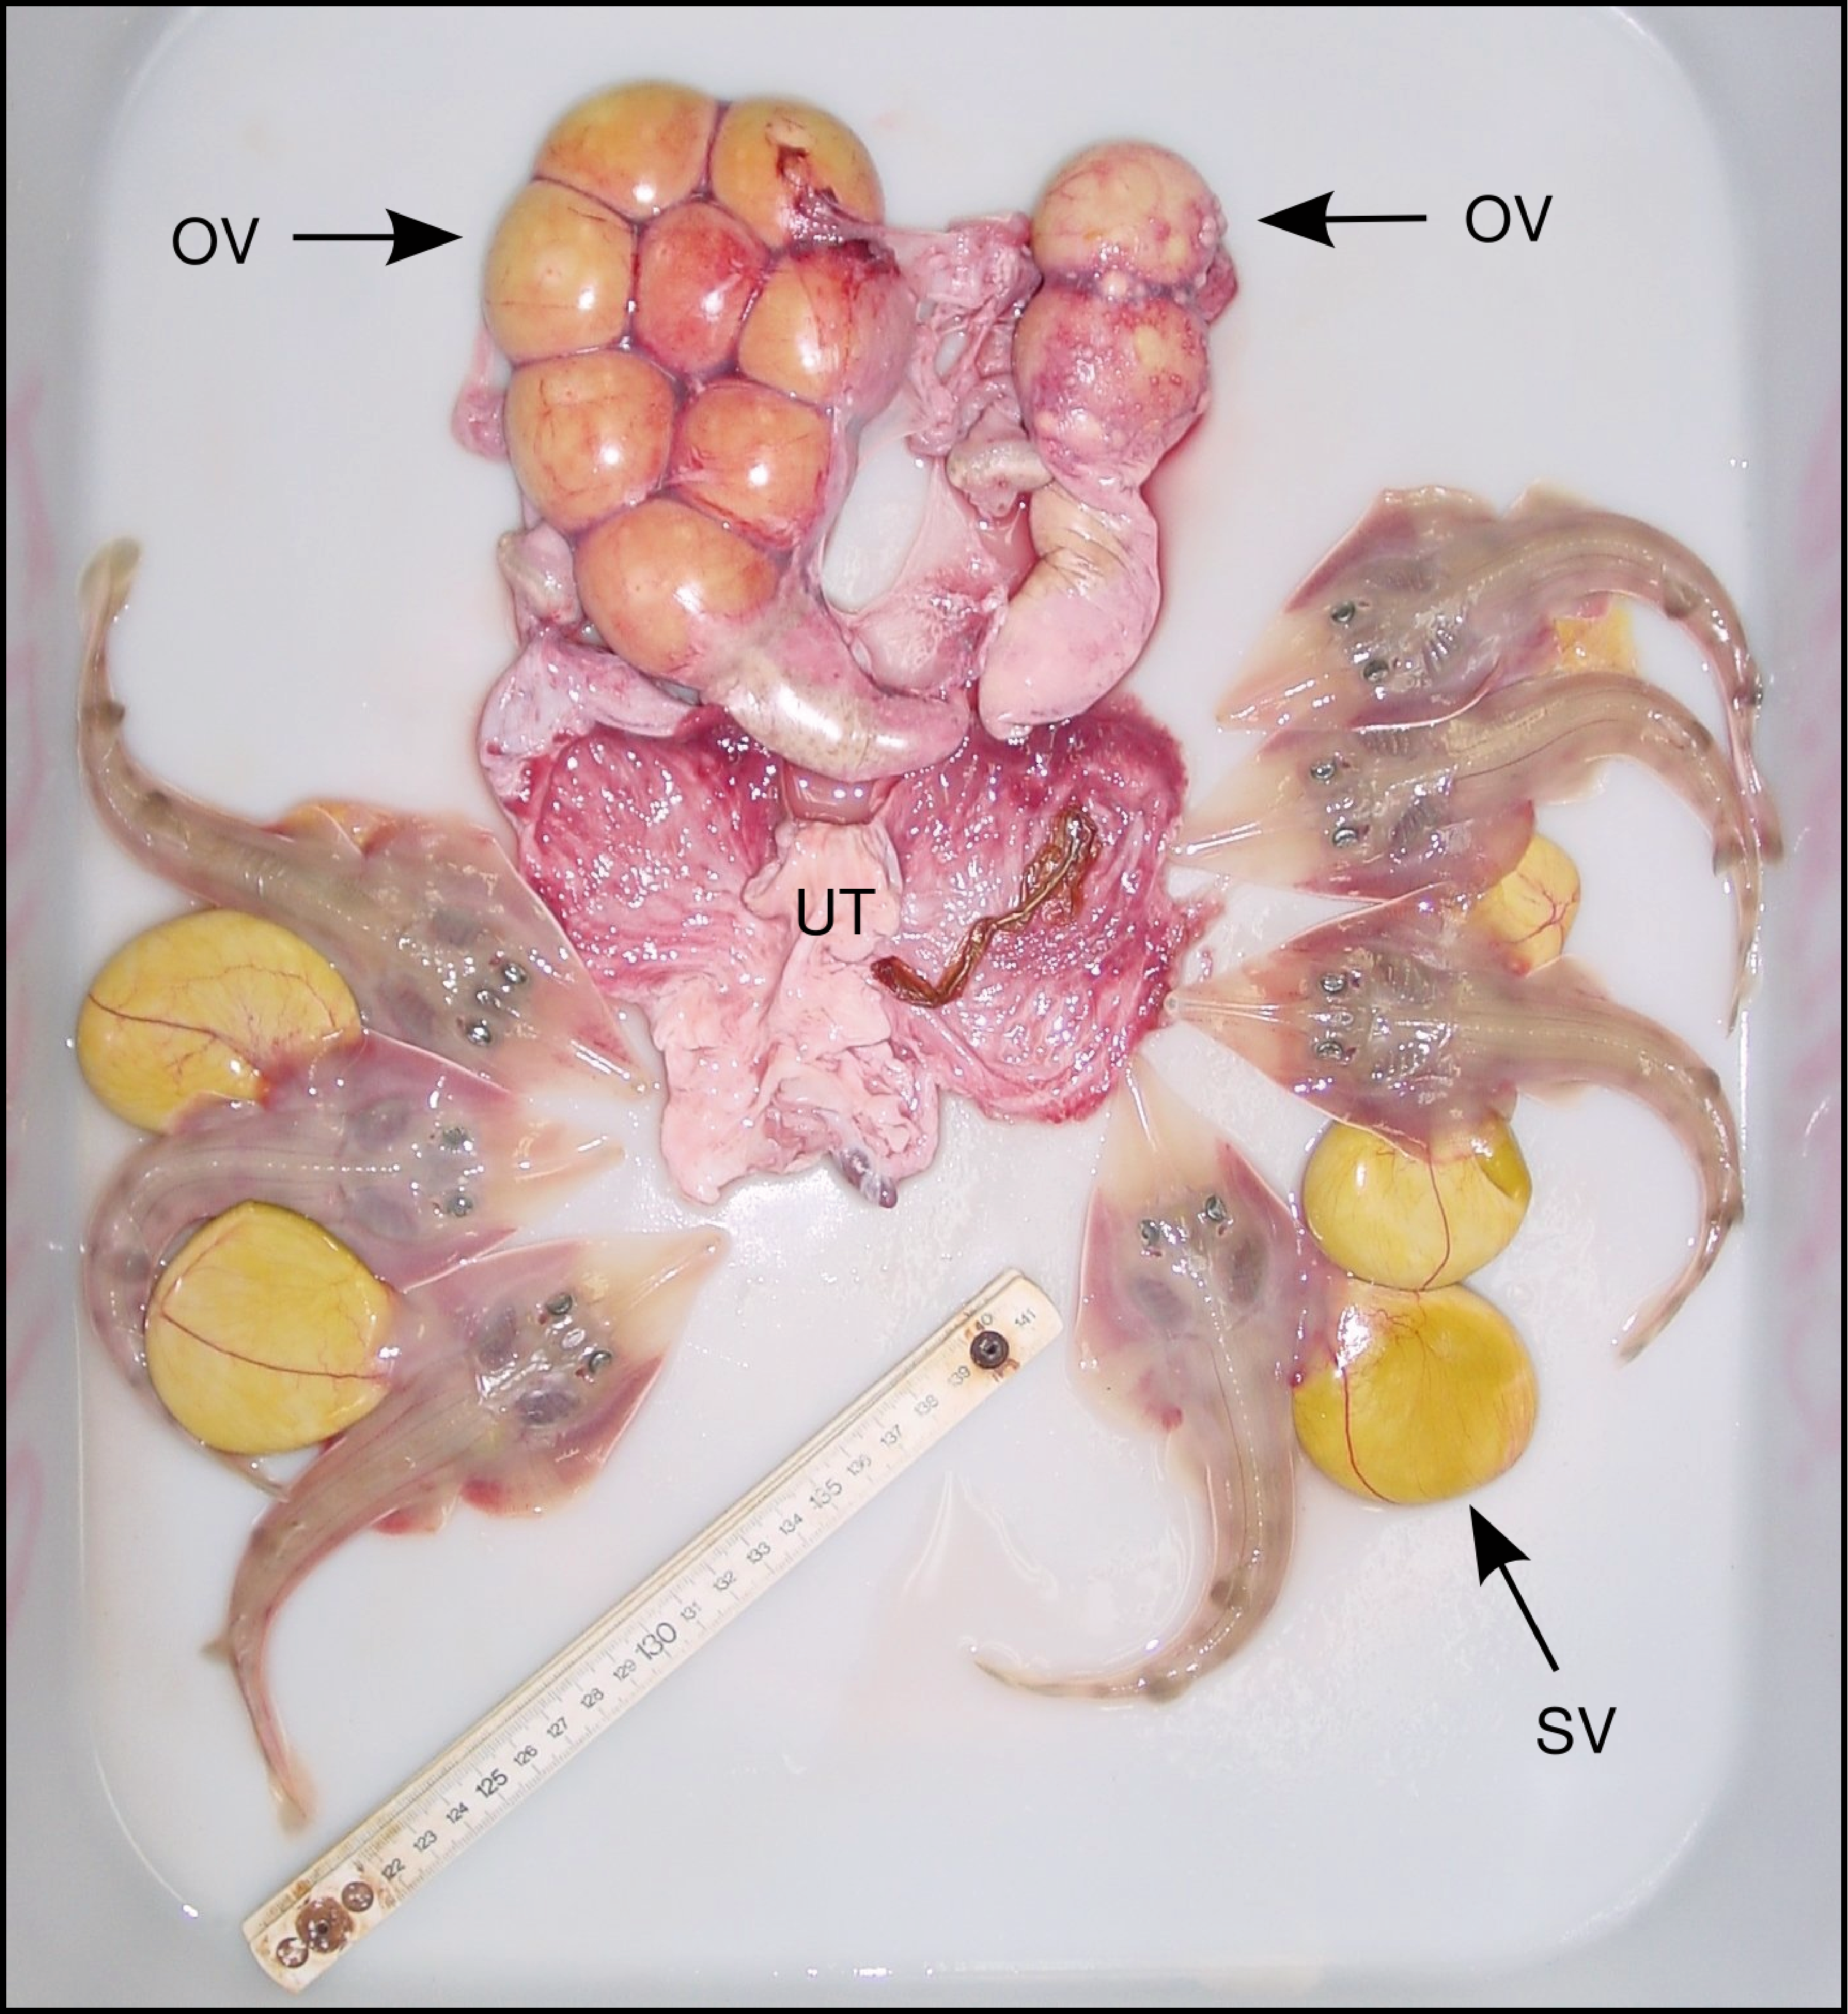
\includegraphics[width=\textwidth]{VIOLA_UTERO}
\end{center}
\caption[Órgãos reprodutivos de uma fêmea prenhe da viola \emph{Rhinobatos horkelii}]
	{Os órgãos reprodutivos de uma fêmea prenhe da viola \emph{Rhinobatos horkelii}
	 capturada na Praia do Cassino em fevereiro de 2003, com os dois ovários, os dois úteros  
	 abertos e os embriões de cada útero. Os ovários contém dez ovócitos em maturação. OV = ovário, UT = útero, SV = saco vitelínico do embrião.}
\label{fig:foto-embrioes-viola}
\end{figure}

%%%

Na Plataforma Sul o ciclo reprodutivo da viola é anual no nível do indivíduo e 
sincronizado no nível da população, o que significa que todas as fêmeas adultas 
dão à luz na mesma época do ano. Durante a gestação ocorre a maturação 
dos ovócitos, e no momento do parto a fêmea possui os ovócitos já prontos para 
sua próxima ninhada.    Logo após o parto, que acontece nos meses de fevereiro 
e março, a fêmea copula e engravida novamente. Em todos os momentos, todas 
as fêmeas adultas estão prenhes, exceto durante o breve intervalo de tempo 
para a cópula, entre o parto e a gravidez subseqüente \citep{lessa1986}. % (Lessa et al., 1986). 

O número de filhotes produzidos a cada gestação aumenta com o tamanho da mãe, 
desde três na fêmea com CT de 90~cm, até 12 na fêmea de 135~cm (Tabela~\ref{tab:parametros-populacionais-viola}). 
O tamanho corporal ao nascer situa-se no intervalo entre o CT do menor 
neonato capturado, que foi de 22~cm no Cruzeiro SALVAR, e do maior embrião 
encontrado, que foi de 29~cm segundo \citet{lessa1982}. A variação do CT e do 
peso dos neonatos pode estar relacionada com a amplitude do CT das fêmeas 
reprodutoras, de 91 a 135~cm (Tabela~\ref{tab:parametros-populacionais-viola}).
Talvez as fêmeas maiores produzem maiores neonatos.

\section*{As migrações sazonais da viola na Plataforma Sul}

\emph{Rhinobatos horkelii} ocorre em todas as profundidades menores que 180~m (Figura~\ref{fig:fo-viola-profundidade}). 
A variação sazonal da relação entre a profundidade e a CPUE dos cruzeiros 
de pesquisa é evidência de migrações sazonais entre zonas de profundidade (Figura~\ref{fig:viola-cpueportrimestre}). 
No inverno a biomassa é distribuída principalmente nas profundidades de 50 a 150~m, 
com elevadas densidades nas profundidades maiores que 100~m. Na primavera começa  
a migração para as águas costeiras, e no verão a biomassa da população está 
concentrada nas profundidades menores que 20~m. No outono, a população começa 
a migrar para fora, e sua biomassa distribui-se nas profundidades de 20 a 100~m. 
O fato de que esse padrão foi observado tanto ao norte como ao sul da latitude 
de Rio Grande é evidência de que a migração sazonal entre profundidades ocorre 
ao longo da costa da Plataforma Sul (Figura~\ref{fig:viola-mapacpue}). 
No inverno o centro da distribuição da biomassa é a plataforma média e externa 
entre as latitudes de 31°30'S e 33°00'S. Essa distribuição sazonal da biomassa 
corresponde com o padrão sazonal da pesca da viola pela frota de arrasto simples 
e arrasto duplo de Itajaí. Nos anos de 2000 a 2002, os barcos dessa frota obtiveram suas 
capturas de viola no outono e inverno principalmente na plataforma externa entre 
Mostardas e Rio Grande \citep{martins2003}. % (Martins e Schwingel, 2003).
A frota de arrasto simples do porto de Rio Grande opera principalmente 
na plataforma média e externa entre Mostardas e Chuí e também obtém suas 
maiores capturas de viola nos meses de abril a setembro \citep[Capítulo~\ref{chap:pesca-industrial}]{miranda2003}. % (Miranda e Vooren, 2003). 
Recentemente a frota de arrasto simples de Itajaí obteve no inverno importantes 
capturas da viola também na plataforma externa entre o Cabo de Santa Marta Grande 
e Tramandaí, que portanto é outra área de invernagem 
da viola da Plataforma Sul \citep{martins2003}. % (Martins e Schwingel, 2003). 

%
% HISTOGRAMA COM A OCORRÊNCIA DA VIOLA POR PROFUNDIDADE
%
%%%%%%%%%%%%%%%%%%%%%%%%%%%%%%%%%%%%%%%%%%%%%%%%%%%%%%%%%%%%%%%

\begin{figure}
\begin{center}
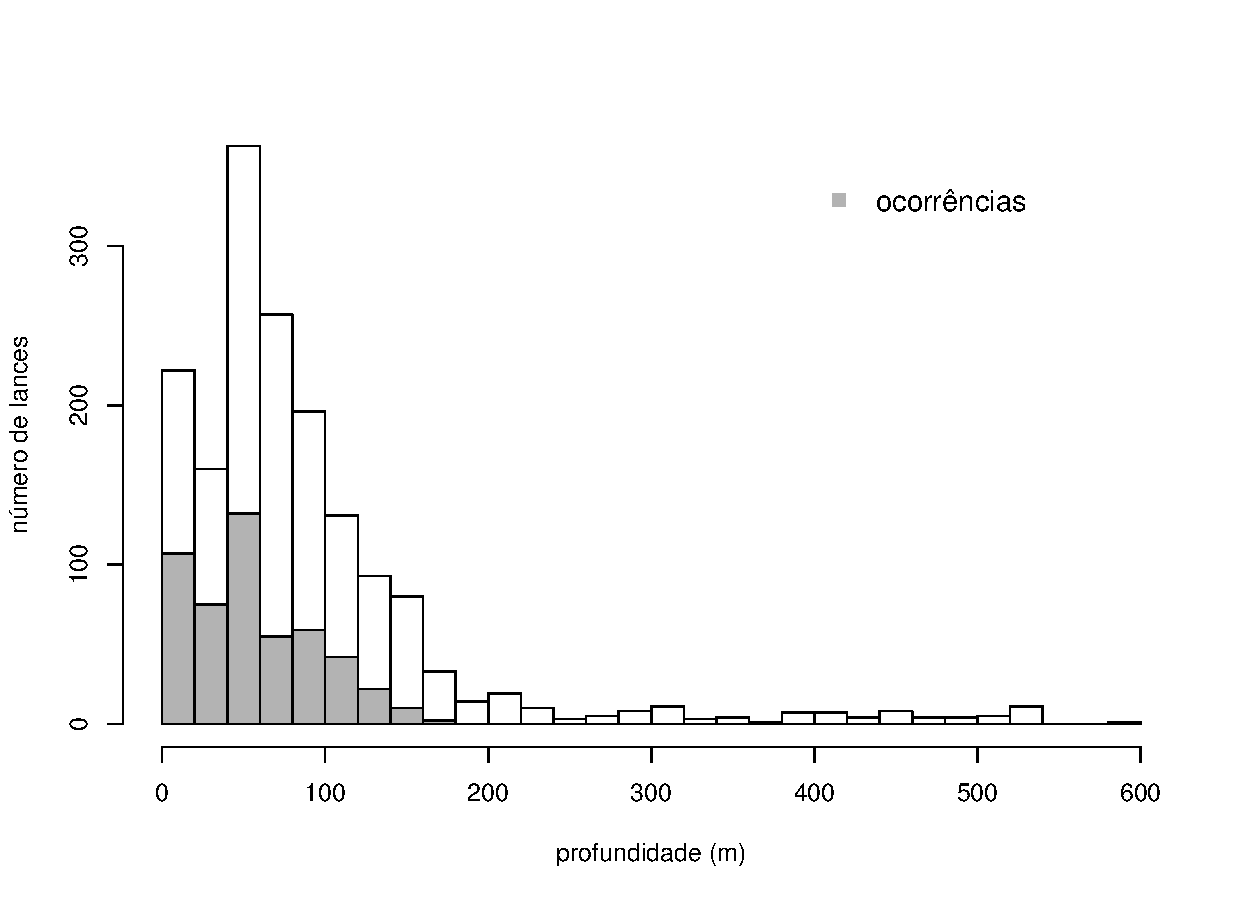
\includegraphics[width=\textwidth]{VIOLA_DISTRIBPROF}
\end{center}
\caption[A freqüência de ocorrência da viola \emph{Rhinobatos horkelii} 
	em relação com a profundidade, nas estações de arrasto de 
	fundo na Plataforma Sul nos anos 1972--2005]
	{A freqüência de ocorrência da viola \emph{Rhinobatos horkelii} 
	em relação com a profundidade, nas estações de arrasto de 
	fundo na Plataforma Sul nos anos 1972--2005. 
	As barras cheias denotam presença da espécie, 
	as barras vazias denotam sua ausência.}
\label{fig:fo-viola-profundidade}
\end{figure}

%%%

%
% VARIAÇÃO SAZONAL DA CPUE (Kg/h)
%
%%%%%%%%%%%%%%%%%%%%%%%%%%%%%%%%%%%%%%%%%%%%%%%%%%%%%%%%%%%%%%%

\begin{figure}
\begin{center}
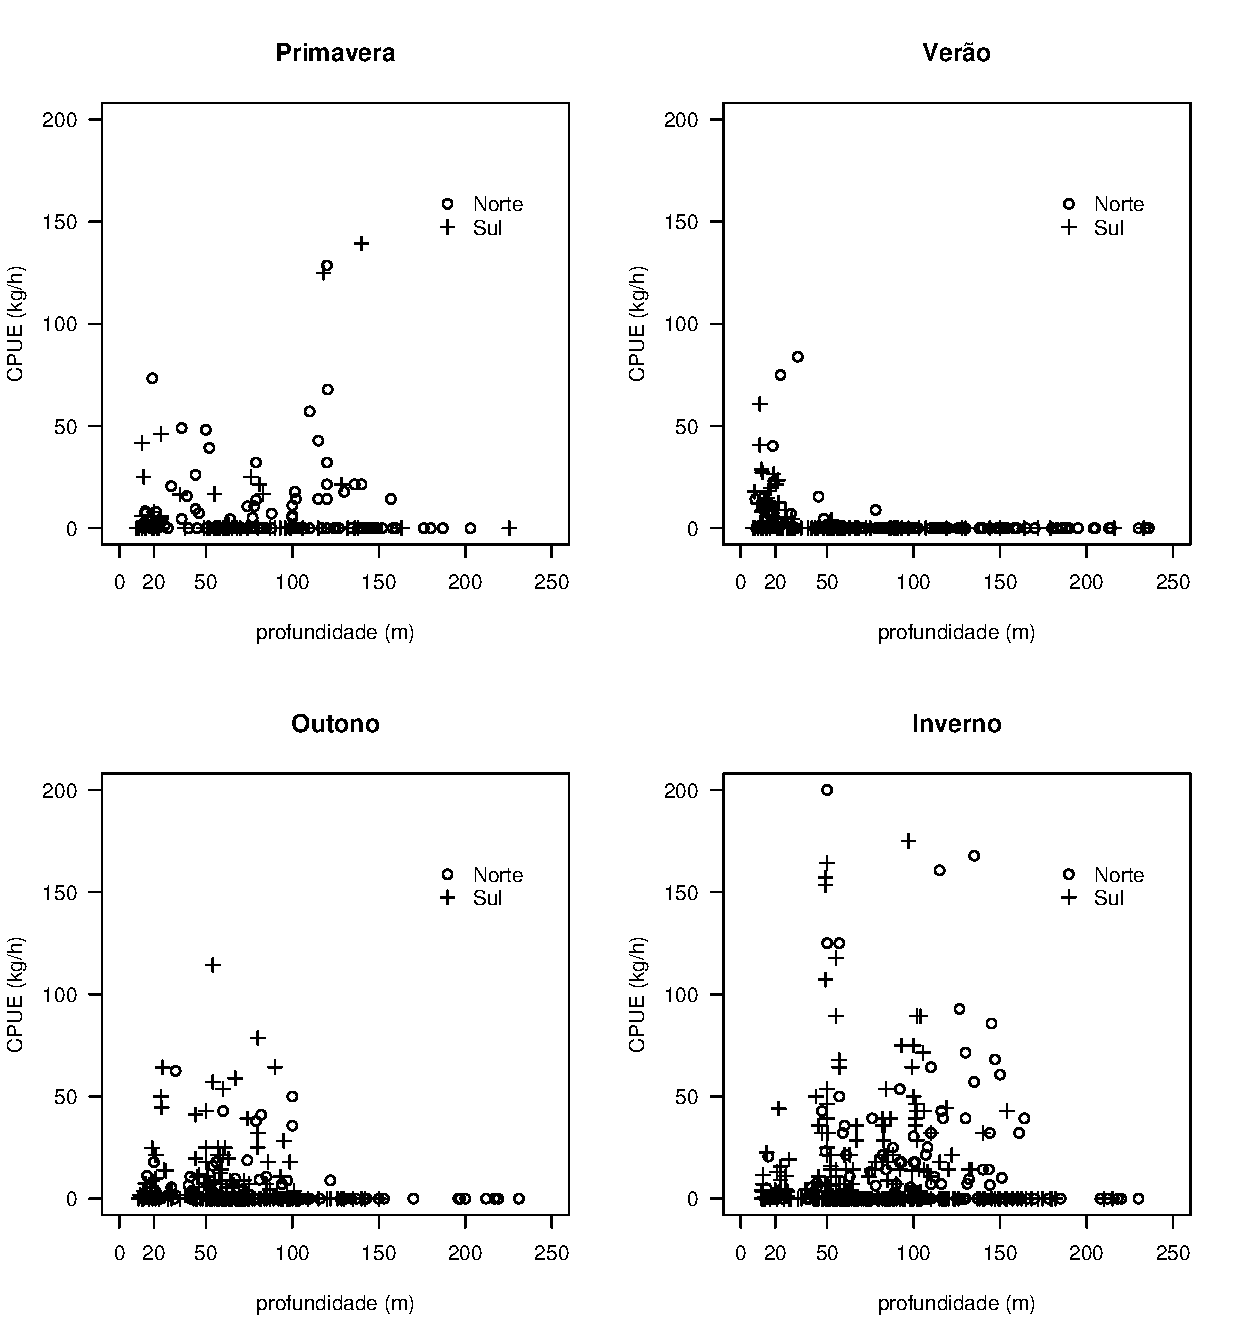
\includegraphics[width=\textwidth]{VIOLA_CPUEXPROFTRIMESTRES}
\end{center}
\caption[Variação sazonal da densidade populacional da viola \emph{Rhinobatos horkelii}]
	{A variação sazonal da densidade populacional da viola \emph{Rhinobatos horkelii} 
	 nas diferentes profundidades da Plataforma Sul, ao norte e ao sul de Rio Grande. 
	 Cada ponto é a Captura por Unidade de Esforço (CPUE) em kg/hora, de uma 
	 estação de pesca de arrasto de fundo nos anos de  1972--2005.}
\label{fig:viola-cpueportrimestre}
\end{figure}

%%%

%
% MAPAS COM DISTRIBUIÇÃO ESPACIAL DA CPUE DA VIOLA
%
%%%%%%%%%%%%%%%%%%%%%%%%%%%%%%%%%%%%%%%%%%%%%%%%%%%%%%%%%%%%%%%

\begin{figure}
\begin{center}
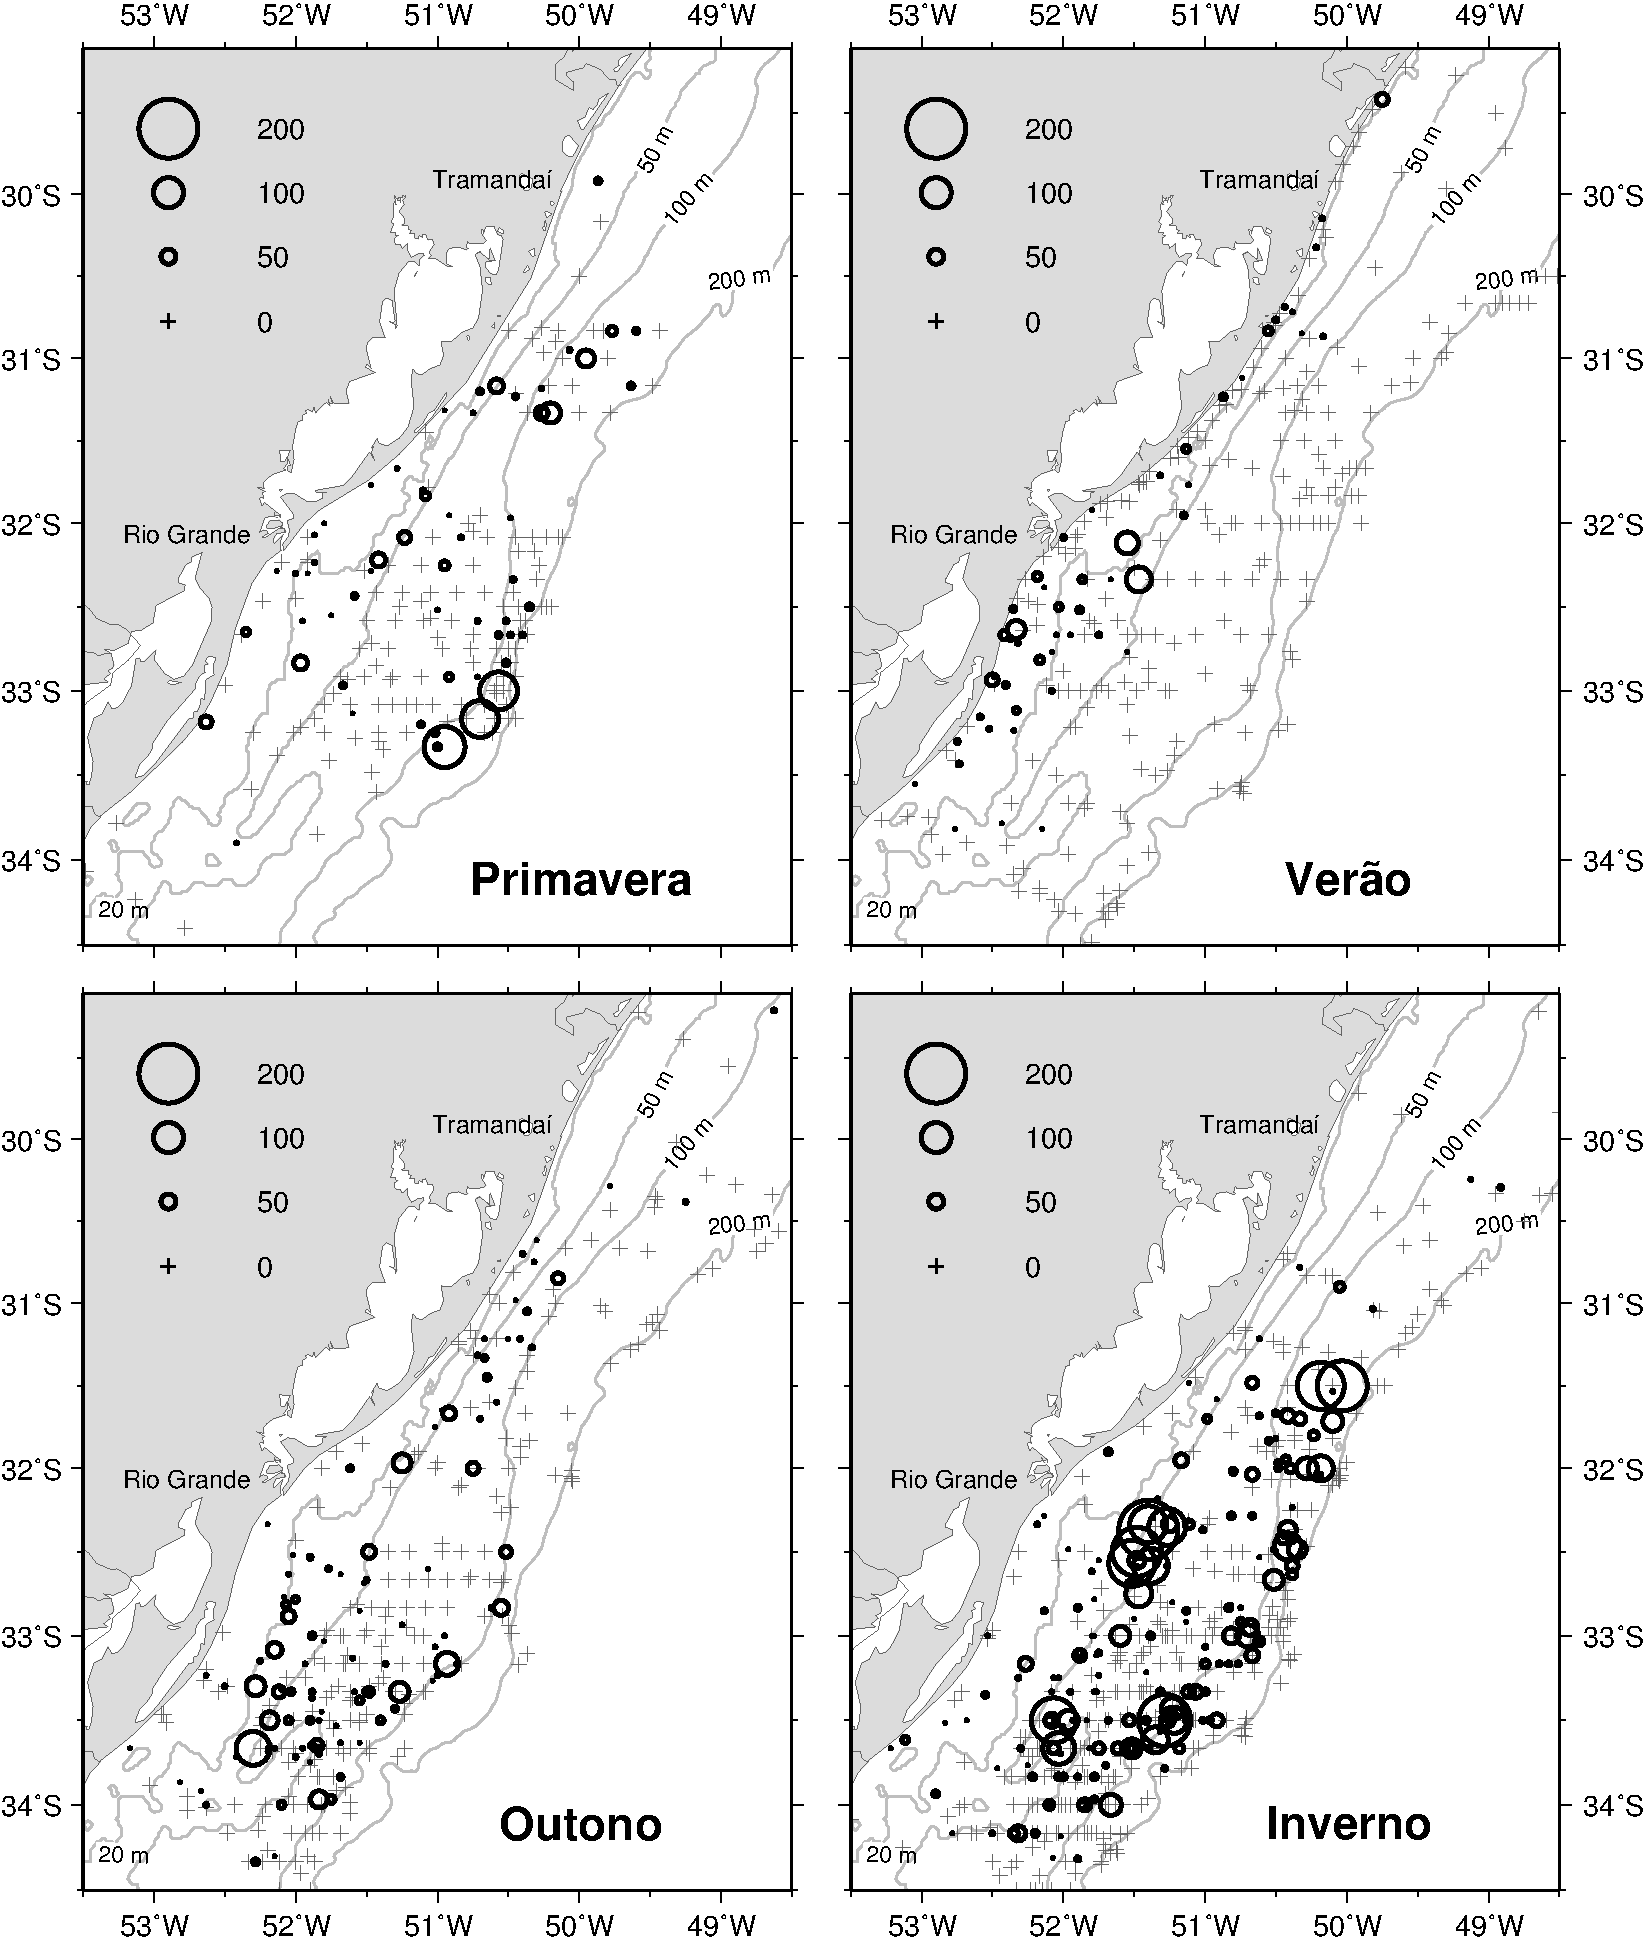
\includegraphics[width=\textwidth]{VIOLA_MAPA_DISTRIBUICAO_CPUE}
\end{center}
\caption[Variação sazonal da distribuição espacial da CPUE em kg/hora, da viola \emph{Rhinobatos horkelii}]
	{A variação sazonal da distribuição espacial da CPUE em kg/hora, da viola \emph{Rhinobatos horkelii} 
	 na Plataforma Sul, nos levantamentos com arrasto de fundo nos anos de 1972--2005. 
	 As cruzes indicam as posições das estações de arrasto de fundo sem captura da espécie.}
\label{fig:viola-mapacpue}
\end{figure}

%%%

Fêmeas com CT maior que 100~cm e machos com CT  maior que 80~cm foram abundantes nas 
capturas comerciais da viola com o arrastão de praia ao sul de Rio Grande nos meses 
de primavera a outono dos anos de 1980 e 1981, e foram quase ausentes das capturas de inverno (Figura~\ref{fig:viola-hist-ct1980}). 
Isto é evidência de que  a migração sazonal para as águas costeiras é realizada pelos adultos 
de ambos os sexos, como também afirma \citet{lessa1982}. % Lessa (1982). % <- referência tese
A fêmea prenhe chega nas águas 
costeiras em novembro ou dezembro, quando então começa o desenvolvimento acelerado dos embriões. 
A fêmea dá à luz em fevereiro 
ou março e logo em seguida passa pela seqüência da cópula, da ovulação e da fecundação dos óvulos. 
Após esta seqüência de atividades reprodutivas nas águas costeiras, a fêmea migra para a plataforma 
externa, prenhe de ovos que permanecem dormentes até que a fêmea retorna para a costa na 
primavera seguinte \citep{lessa1982}. % <- referência tese
Os machos adultos aparecem no verão e ainda permanecem em grande número no outono (Figura~\ref{fig:viola-hist-ct1980}). 
A migração dos machos adultos para as águas costeiras nos meses de verão e outono ocorre em 
função da cópula. A pesca de verão nas águas costeiras incide sobre os adultos de ambos os 
sexos em momentos críticos da reprodução. 

%
% HISTOGRAMAS POR EPOCA NO ARRASTAO DE PRAIA 1979-1981
%
%%%%%%%%%%%%%%%%%%%%%%%%%%%%%%%%%%%%%%%%%%%%%%%%%%%%%%%%%%%%%%%

\begin{figure}
\begin{center}
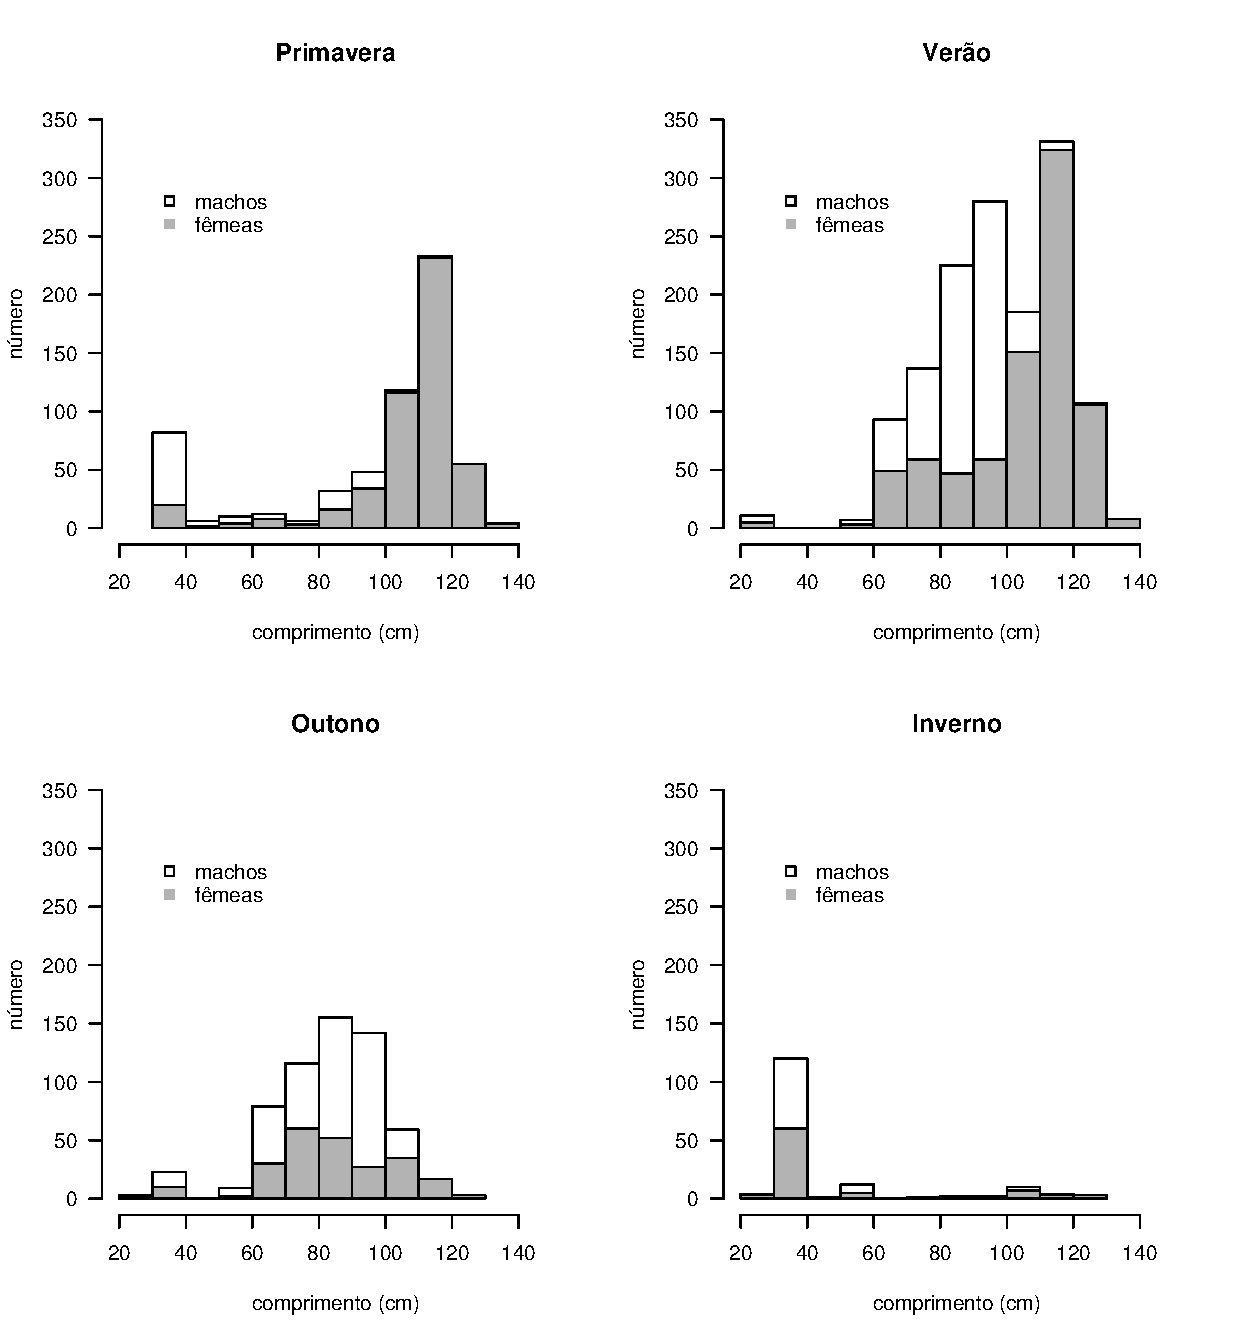
\includegraphics[width=\textwidth]{VIOLA_CTXEPOCAS}
\end{center}
\caption[Composição das capturas da viola \emph{Rhinobatos horkelii}
	 pela pesca artesanal com arrastão de praia na costa do Rio Grande do Sul]
	{Composição das capturas da viola \emph{Rhinobatos horkelii}
	 pela pesca artesanal com arrastão de praia na costa do Rio Grande do Sul, 
	 entre Cassino e Albardão, nos anos  1979-1981. Os dados de primavera são dos meses de novembro e dezembro.  
	 Fonte: dados pretéritos coletados por 
	 Rosângela Paula Lessa e Carolus Maria Vooren.}
\label{fig:viola-hist-ct1980}
\end{figure}

%%%

Fêmeas jovens com CT de 60 a 99~cm e machos jovens com CT de 60 a 79~cm foram 
também abundantes nas capturas com o arrasto de praia no verão, e quase ausentes 
das capturas de inverno (Figura~\ref{fig:viola-hist-ct1980}). 
A viola da Plataforma Sul alcança o CT de 61~cm com a idade de 2 anos \citep{lessa1982}. % (Lessa, 1982).  
A composição das capturas de verão é evidência de que no final do segundo ano de vida 
os juvenis da viola começam a participar da migração sazonal entre as águas costeiras 
e as maiores profundidades da plataforma. A pesca de verão nas águas costeiras incide 
também sobre os juvenis da viola.

% Nos anos de 2002 e 2003 as capturas das pescarias que operam freqüentemente em 
% águas costeiras foram principalmente de indivíduos jovens com CT de menos de 90~cm, 
% enquanto uma grande proporção das capturas do arrasto simples, que opera mais na 
% plataforma média e externa, foi de fêmeas adultas com CT de 90 a 130~cm (Capítulo~?, Figura~\ref{fig:ct-viola}). % CT viola pesca industrial
% Isto é confirmação da maneira como a viola se distribui sobre a plataforma, e demonstra 
% o impacto das pescarias sobre a viola nas diferentes fases do ciclo de vida dessa espécie.

Na Plataforma Sul, a temperatura de fundo varia entre profundidades 
e ainda sazonalmente. Nas águas costeiras rasas, a variação sazonal da temperatura do 
ar e da insolação resulta em elevada variação sazonal da temperatura de fundo, entre 
cerca de 13°C no inverno e 22 a 24°C no verão na profundidade de 10~m (Figura~\ref{fig:temperatura-sup-e-fundo}). % Sazonalidade da temperatura capitulo hidrografia
Ao norte da latitude do Farol de Sarita (32°30'S) a amplitude da  variação sazonal 
é menor na plataforma interna, com temperaturas de fundo de 13 a 18°C no inverno 
e  17 a 18°C no verão nas profundidades de 50 a 100~m, enquanto na plataforma externa 
a temperatura de fundo é de 15 a 16°C ao longo do ano 
na profundidade de 180~m \citep{CASTELLO1977,castro1998}.
Em virtude dessa estrutura térmica do ambiente bentônico da plataforma, um indivíduo 
de \emph{R. horkelii} que realiza a migração sazonal experimenta uma variação 
de temperatura de até 11°C,  entre valores de 13 a 18°C no inverno e 
de 22 a 24°C no verão (Figura~\ref{fig:viola-distrib-tempfundo}). 
Isto corrobora a conclusão de \citet{lessa1986} % Lessa et al. (1986) 
de que a migração das fêmeas prenhes para as águas costeiras 
no verão está relacionada com as elevadas 
temperaturas necessárias para o rápido desenvolvimento do embrião durante o verão, 
enquanto as baixas temperaturas do hábitat de inverno na plataforma externa são 
necessárias para a dormência do ovo no útero. Pela sua migração sazonal, a fêmea 
prenhe regula sua temperatura corporal e com isto, ela controla o cronograma da 
gestação de tal maneira que sua prole nasce no verão nas águas costeiras que são 
o hábitat específico dos neonatos. Isto significa que não somente o berçário costeiro, 
mas também a plataforma externa é uma área crítica para a reprodução de \emph{R. horkelii}. 
O deslocamento do esforço de pesca da frota de Itajaí de arrasto simples e arrasto duplo 
para a plataforma externa, que segundo \citet{martins2003} % Martins e Schwingel (2003) 
ocorreu nos anos de 2000 a 2002, causou um impacto sobre 
uma área crítica de \emph{R. horkelii}.

%
% FO DA VIOLA POR TEMPERATURA DE FUNDO
%
%%%%%%%%%%%%%%%%%%%%%%%%%%%%%%%%%%%%%%%%%%%%%%%%%%%%%%%%%%%%%%%

\begin{figure}
\begin{center}
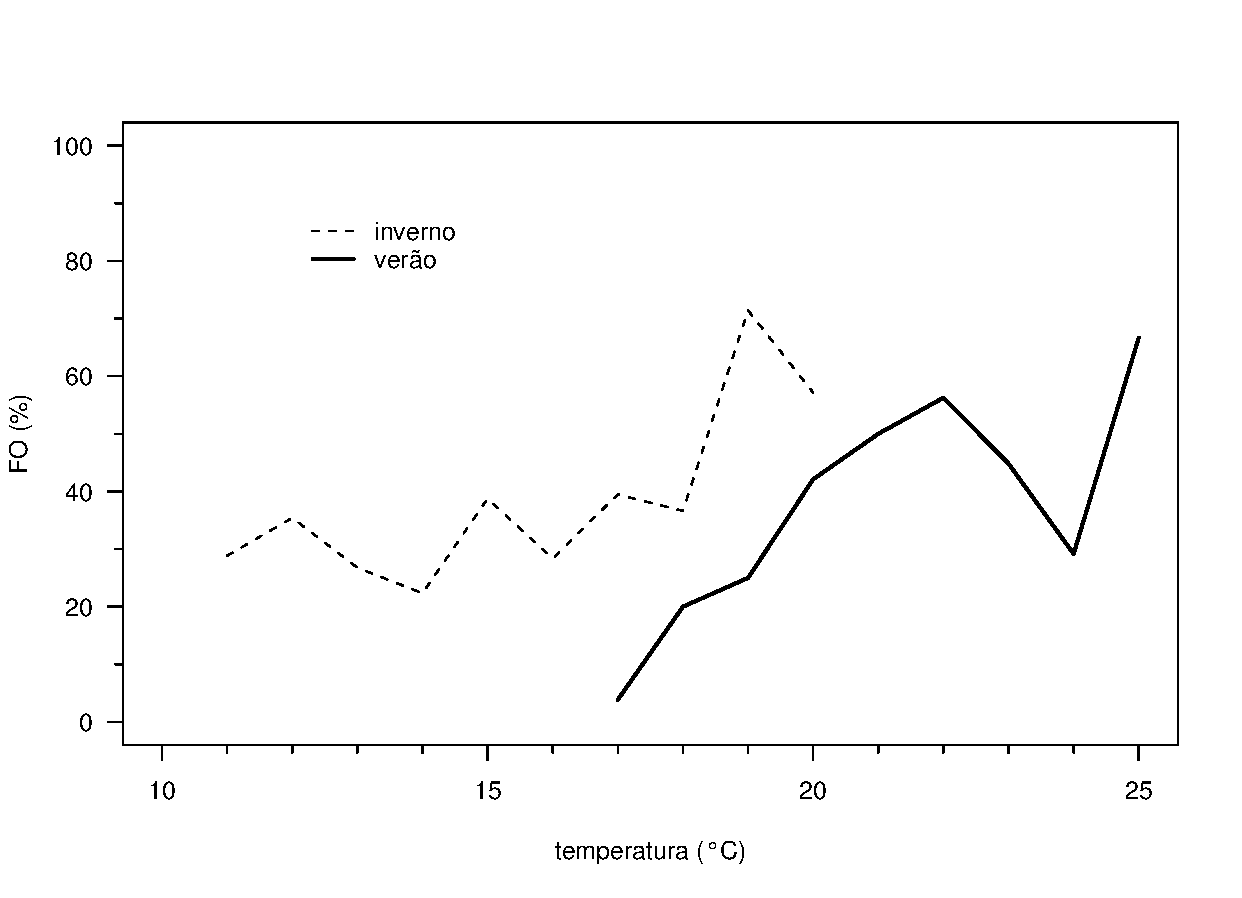
\includegraphics[width=\textwidth]{VIOLA_DISTRIBTEMPFUNDO}
\end{center}
\caption[Freqüência de ocorrência (FO) da viola \emph{Rhinobatos horkelii} 
	 com relação à temperatura de fundo]
	{Freqüência de ocorrência (FO) da viola \emph{Rhinobatos horkelii} 
	 com relação à temperatura de fundo, nos levantamentos com 
	 arrasto de fundo nos anos 1980--2005.}
\label{fig:viola-distrib-tempfundo}
\end{figure}

%%%

A variação sazonal da temperatura de fundo é maior  na área sul da plataforma, 
entre as latitudes do Farol da Verga (33°00'S) e Chuí, onde no inverno predominam 
temperaturas de 11 a 12°C, devido à maior influência da Corrente das Malvinas nessa área \citep{HAIMOVICI1994B}. % (Haimovici, 1995). 
Isto pode ser o fator que determina que no inverno a maior densidade da viola
ocorre ao norte dessa área ou seja, na plataforma média e externa entre as 
latitudes de 32°30'S e 33°00'S (Figura~\ref{fig:viola-mapacpue}). 

\section*{O berçário da viola nas águas costeiras da Plataforma Sul}

Neonatos da viola são definidos como indivíduos com CT no intervalo de 20 a 40~cm. 
Essa categoria constitui o conjunto dos indivíduos que nascem no verão e cujo CT  
aumenta desde o CT ao nascer que é em torno de 25~cm, até o CT 
de cerca de 40~cm no final do seu primeiro ano de vida. Neonatos foram capturados com 
o arrastão de praia  ao longo do ano (Figura~\ref{fig:viola-hist-ct1980}). 
No verão,  os neonatos estavam todos 
no intervalo de CT de 20 a 30~cm. Isto reflete o nascimento da nova coorte. 
De outono a primavera predominaram neonatos com CT no intervalo de 30 a 40~cm.  
Isto reflete o crescimento corporal da coorte durante o primeiro ano de vida. 
Nos anos de 1981 a 1985 entre Rio Grande e Albardão, neonatos da viola foram 
capturados em 6 de 15 lances observados com o arrastão de praia. Em outubro de 1981 
foram capturados respectivamente 17 e 30 neonatos com CT de 36 a 40~cm em dois lances 
de arrastão no balneário Cassino. Os neonatos da viola permanecem nas águas 
costeiras da Plataforma Sul durante o primeiro ano de vida, e neonatos eram comuns 
e abundantes nessas águas na década de 1980. 

Nos levantamentos pretéritos com arrasto de fundo e no Cruzeiro SALVAR em conjunto, 
as nove ocorrências de neonatos são distribuídas ao longo de toda 
a costa ao sul da latitude de 30°00'S e somente nas águas costeiras 
com profundidades de cerca de 10~m que foram as menores profundidades 
amostradas nesses levantamentos (Figura~\ref{fig:viola-mapa-neonatos}). 
Isto  corrobora que a migração reprodutiva das fêmeas prenhes para as 
águas rasas ocorre ao longo dessa costa. Os dados sobre a distribuição espacial 
da biomassa e dos neonatos e sobre a população amostrada com o arrastão de praia 
(Figuras~\ref{fig:viola-mapacpue}, \ref{fig:viola-hist-ct1980} e \ref{fig:viola-mapa-neonatos}) 
constituem em conjunto a evidência de que nas águas costeiras da Plataforma Sul, 
a população adulta da espécie realiza os processos da gestação, do parto e da cópula nos 
meses de primavera e verão, e de que os neonatos permanecem concentrados nessas águas 
durante o primeiro ano da vida. A zona de águas costeiras da Plataforma Sul é uma área 
crítica para a reprodução e o recrutamento de \emph{R. horkelii}. 

%
% MAPA COM OCORRÊNCIAS DE NEONATOS
%
%%%%%%%%%%%%%%%%%%%%%%%%%%%%%%%%%%%%%

\begin{figure}
\begin{center}
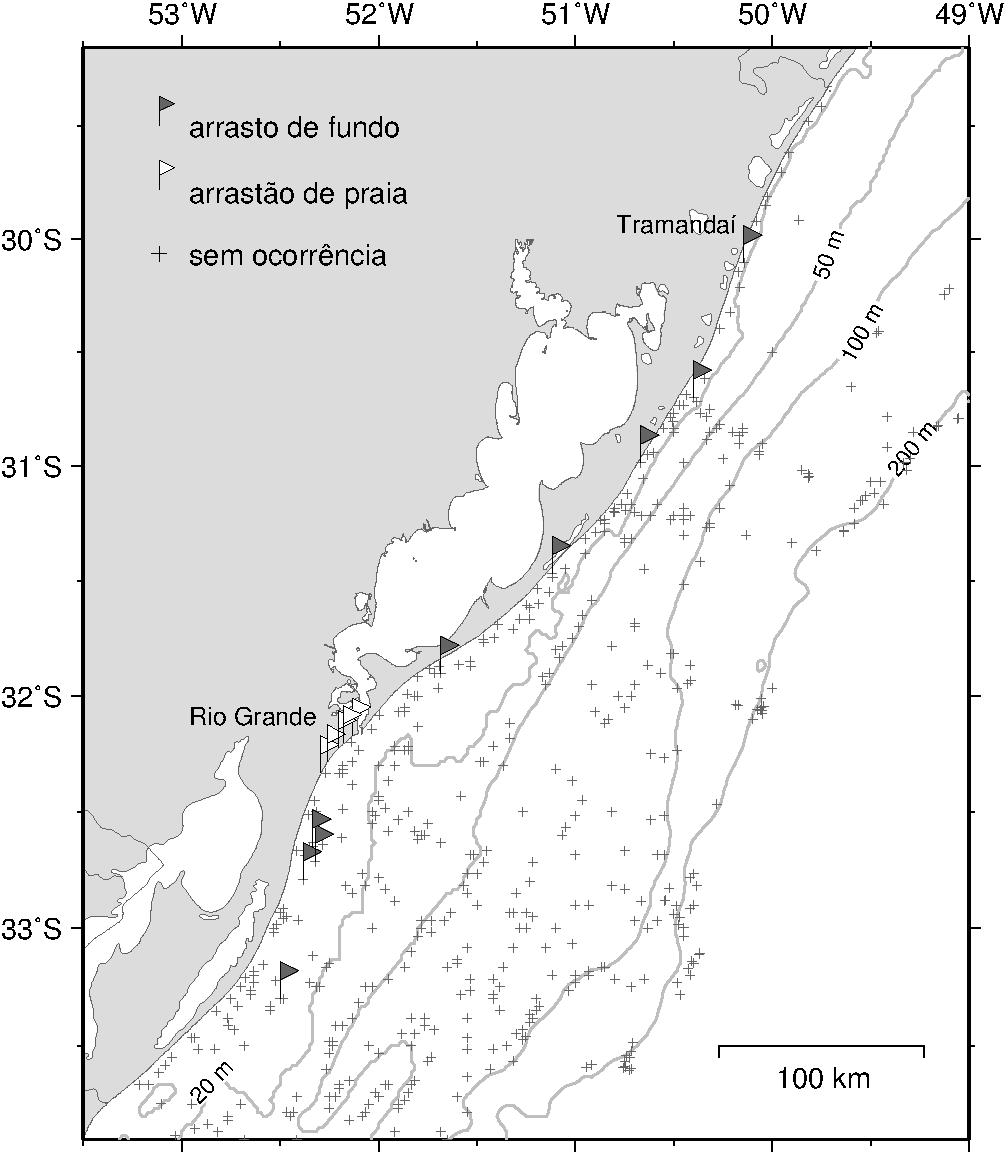
\includegraphics[width=\textwidth]{VIOLA_MAPA_NEONATOS}
\end{center}
\caption[Ocorrências de neonatos da viola \emph{Rhinobatos horkelii} na Plataforma Sul]
	{Ocorrências de neonatos da viola \emph{Rhinobatos horkelii} na Plataforma Sul, 
	 nas estações de pesca com arrasto de fundo do Cruzeiro SALVAR em 2005 e 
	 dos levantamentos pretéritos em 1980--1984, e nas capturas da pesca artesanal 
	 com arrastão de praia nos anos 1979-1981.}
\label{fig:viola-mapa-neonatos}
\end{figure}

%%%

Neonatos da viola foram capturados apenas esporadicamente nos 
levantamentos realizados nos anos de 1980 a 1984 e no Cruzeiro SALVAR, 
apesar do elevado esforço de amostragem desses levantamentos (Figura~\ref{fig:viola-mapa-neonatos}). 
Os levantamentos pretéritos foram realizados com redes de arrasto de fundo 
para a captura de peixes, e essas redes tendem a ser ineficientes para a 
captura de neonatos de raias em geral \citep{oddone2004}. % (Oddone e Vooren, 2004). 
Por este motivo o Cruzeiro SALVAR foi realizado com uma rede de arrasto 
para camarão. Grandes capturas de neonatos das raias \emph{Sympterigia acuta}
e \emph{Sympterigia bonapartii} foram evidência da eficiência dessa rede para 
a captura de neonatos de raias em geral (Capítulo~\ref{chap:elasmos}). % ELASMOBRÂNQUIOS EM GERAL NA PLATAFORMA
O Cruzeiro SALVAR foi realizado no mês de fevereiro de 2005, com a premissa 
de que nesse mês o parto da viola estava acontecendo, e as cinco ocorrências 
de neonatos foram uma confirmação dessa premissa. Mesmo com a reduzida 
abundância da espécie no ano de 2005 em comparação com o nível da década 
de 1980, capturas de neonatos seriam freqüentes na pesca com a rede de arrasto 
para camarão no hábitat dos neonatos. No entanto, apenas cinco neonatos da 
viola foram capturados no total de 62 lances com essa rede nas profundidades 
de 7 a 20~m ao longo da costa do Rio Grande do Sul. Conclui-se que o hábitat 
dos neonatos da viola encontra-se nas profundidades menores que 7~m ou seja, 
nas águas imediatamente adjacentes à zona de arrebentação e que não puderam ser 
amostradas com a embarcação utilizada no levantamento. Que neonatos da viola vivem 
nessas águas é comprovado pelas freqüentes capturas desses peixes ao longo do ano 
com o arrastão de praia, que opera nas profundidades de até cerca de 5~m (Figura~\ref{fig:viola-hist-ct1980}).
A elevada eficiência do arrastão de praia para a captura de adultos da viola 
de ambos os sexos no verão é evidência de que naquela época do ano, esses adultos 
também se encontram nas águas imediatamente adjacentes à zona de arrebentação. 
O berçário da viola é a estreita faixa de águas costeiras, com extensão 
transversal da ordem 1.000 a 2.000~m, com profundidade em torno de 5~m, e 
que se estende ao longo da costa da Plataforma Sul à distância de cerca 
de 500 a 1000~m da praia. Nessa estreita área as fêmeas prenhes e os machos 
adultos se concentram nos meses de novembro a março, e os neonatos permanecem 
concentrados nessa mesma área durante o primeiro ano de vida. 

\section*{O status de conservação da viola da Plataforma Sul}

As estatísticas da pesca pela frota do porto de Rio Grande incluem 
cifras mensais da captura de cada categoria taxonômica de peixe e do 
número de viagens de pesca na Plataforma Sul pelas 
frotas de arrasto simples e de arrasto de parelha nos anos de 1975 a 2002. 
Durante esse período as frotas do arrasto simples e do arrasto de parelha 
mantiveram características técnicas e operacionais semelhantes com relação 
a seu esforço de pesca, e cada uma dessas frotas teve seu período fixo de 
maior abundância da viola na sua área de pesca, com a safra da viola nos 
meses de dezembro a março para o arrasto de parelha e nos meses de abril 
a setembro para o arrasto simples \citep{miranda2003}. % (Miranda e Vooren, 2003). 
Portanto, a CPUE anual da viola de cada frota foi calculada para  
seu período da safra da viola. As pescarias mistas com o arrasto simples 
e o arrasto de parelha  registraram altos valores da captura e da CPUE no 
período de 1975 a 1986, e baixos valores no período de 1993 a 1999 
(Figuras~\ref{fig:viola-desembarques-1945a2002}~e~\ref{fig:viola-cpuesafra-1975a2002}, Tabela~\ref{tab:viola-cpuesafra-variacao}).  
No ano de 1984, no período do pico das capturas e da CPUE, a viola constituiu 1,9\% 
da captura total de peixes pelo arrasto simples, enquanto no arrasto de parelha 
essa proporção foi de 3,5\% \citep{miranda2003}. % (Miranda e Vooren, 2003). 
Nos anos de 1990 a 1994, após o declínio das capturas e da CPUE, o percentual 
da viola foi respectivamente de 0,3 e 0,6\% nos referidos 
tipos de pesca com  arrasto \citep{haimovici1997}. % (Haimovici, 1997).
A viola sempre constituiu uma pequena porcentagem da captura total 
nas pescarias com o arrasto de fundo na Plataforma Sul. 
Isto significa que essas pescarias atuavam no hábitat da viola mas 
capturavam a viola na pesca direcionada ao conjunto de abundantes espécies 
de peixes ósseos que também vivem nesse hábitat (Figura~\ref{fig:violas-noarrasto}). 
Isto justifica o uso da CPUE da viola pelo arrasto simples e o arrasto de 
parelha como índice comparativo da abundância da viola na Plataforma Sul 
no período 1975--2001. Os dois conjuntos de dados da CPUE evidenciam 
que após o ano de 1986 ocorreu um declínio de cerca de 84\% da abundância 
da viola, com relação a abundância no período 1975--1986 (Tabela~\ref{tab:viola-cpuesafra-variacao}). 

%
% DESEMBARQUES TOTAIS DA VIOLA EM RG 1945-2002
%
%%%%%%%%%%%%%%%%%%%%%%%%%%%%%%%%%%%%%%%%%%%%%%%%%%%%%%

\begin{figure}
\begin{center}
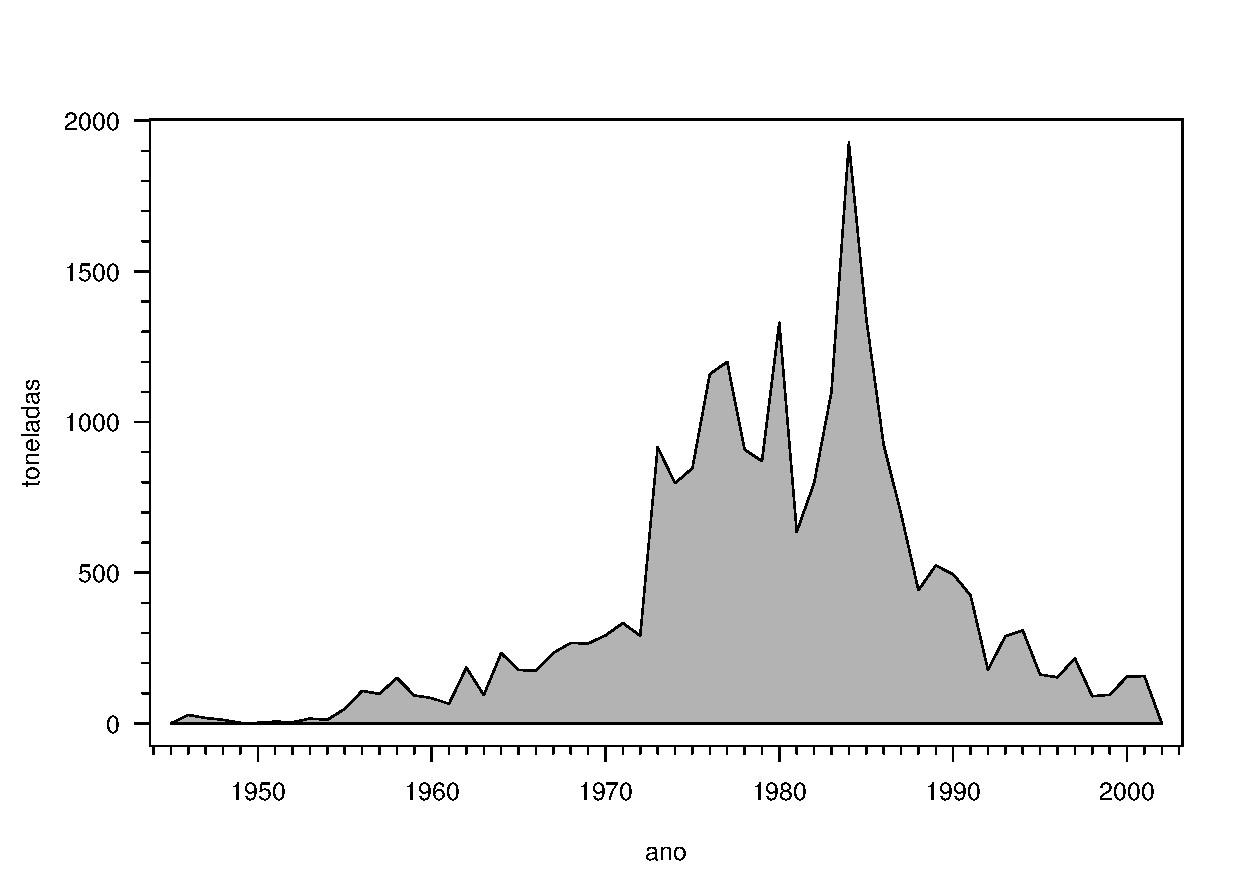
\includegraphics[width=\textwidth]{DESEMBARQUESTOTAISVIOLA}
\end{center}
\caption[Desembarques anuais da viola \emph{Rhinobatos horkelii} entre 1945 e 2002]
	{Desembarques anuais da viola \emph{Rhinobatos horkelii}
	 pela pesca artesanal e industrial no porto de Rio Grande 
	 nos anos de 1945 a 2002. Fonte: IBAMA/CEPERG.}
\label{fig:viola-desembarques-1945a2002}
\end{figure}

%%%

%
% CPUE NA SAFRA DA VIOLA ENTRE 1975 A 2002
%
%%%%%%%%%%%%%%%%%%%%%%%%%%%%%%%%%%%%%%%%%%%%%%%%%%%%%%

\begin{figure}
\begin{center}
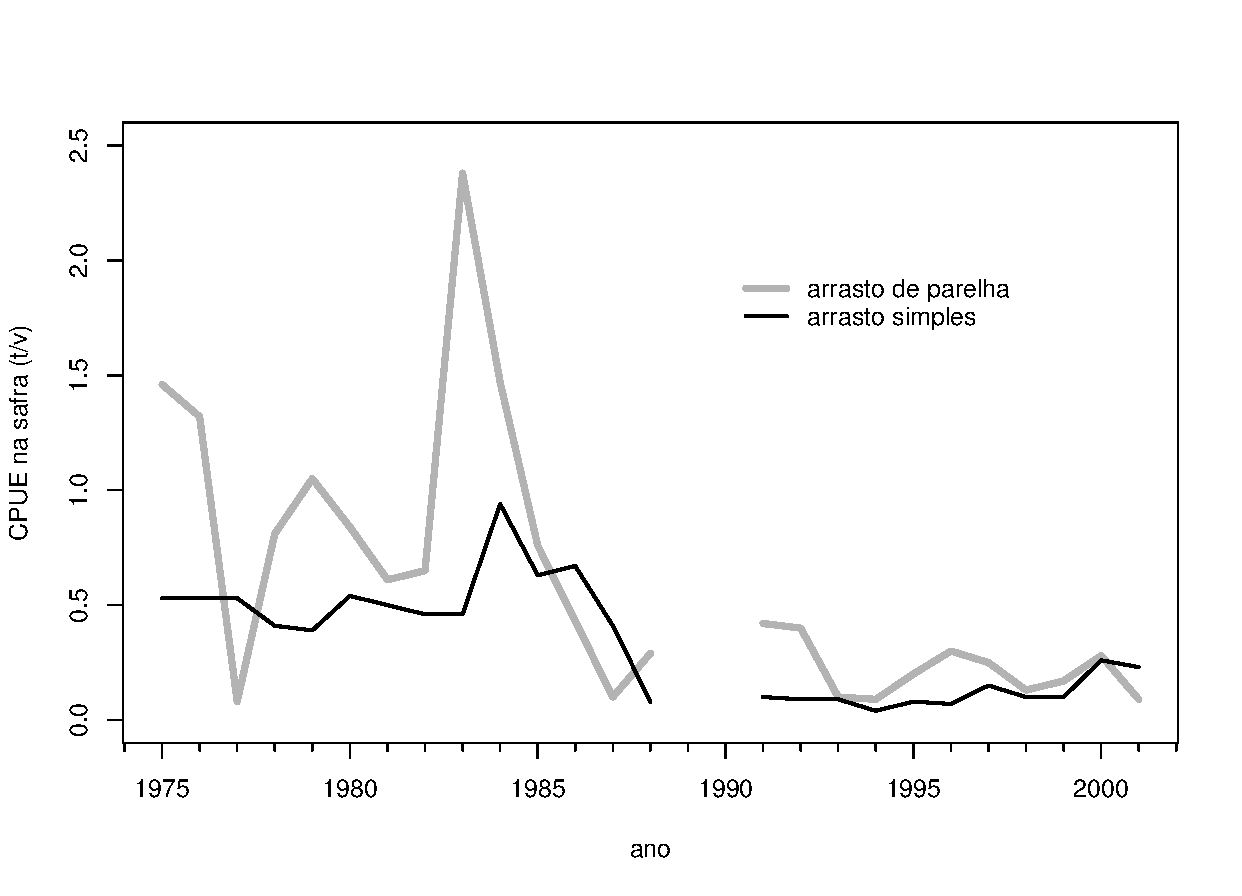
\includegraphics[width=\textwidth]{CPUESAFRAVIOLA}
\end{center}
\caption[Captura por Unidade de Esforço (CPUE) em ton/viagem, 
	 da viola \emph{Rhinobatos horkelii} na Plataforma Sul, 
	 pelas frotas de arrasto simples e arrasto de parelha de Rio Grande]
	{Captura por Unidade de Esforço (CPUE) em ton/viagem, 
	 da viola \emph{Rhinobatos horkelii} na Plataforma Sul, 
	 pelas frotas de arrasto simples (abril-setembro) e arrasto de parelha (dezembro-março)
	 que desembarcaram no porto de Rio Grande. Fontes: \citet{miranda2003} e IBAMA/CEPERG.}
\label{fig:viola-cpuesafra-1975a2002}
\end{figure}

%%%

%
% TABELA VARIAÇÃO DA CPUE NA SAFRA DA VIOLA NO ARRASTO SIMPLES E DE PARELHA
%
%%%%%%%%%%%%%%%%%%%%%%%%%%%%%%%%%%%%%%%%%%%%%%%%%%%%%%%%%%%%%%%%%%%%%%%%%%%%

\begin{table}
\caption[Média e amplitude dos valores anuais da captura por unidade de esforço, 
         em ton/viagem, da viola \emph{Rhinobatos horkelii} pelas frotas de arrasto simples 
	 e arrasto de parelha que desembarcaram no porto de Rio Grande]
        {Média e amplitude dos valores anuais da captura por unidade de esforço, 
         em ton/viagem, da viola \emph{Rhinobatos horkelii} pelas frotas de arrasto simples 
	 e arrasto de parelha que desembarcaram no porto de Rio Grande. 
	 Fontes: \citet{miranda2003} e IBAMA/CEPERG.}
\label{tab:viola-cpuesafra-variacao}
\begin{center}
\begin{tabular*}{\textwidth}{l@{\extracolsep{\fill}}ll}
\toprule
Anos 	& Arrasto simples		& Arrasto de parelha \\
	& safra: abril-setembro		& safra: dezembro-março	\\
\midrule
 1975-1986 (12 anos) & 0,55 (0,41-0,94)	& 1,07 (0,43-2,38)	\\
\addlinespace
 1993-1999 (7 anos)  & 0,09 (0,04-0,15) & 0,18 (0,09-0,30)	\\
\midrule
 93-99 como \% de 75-86 & 16\%		& 17\%			\\
\bottomrule
\end{tabular*}
\end{center}
\end{table}

%%%

A frota do arrasto de parelha opera principalmente na plataforma interna, 
enquanto a frota do arrasto simples opera mais na plataforma externa (Capítulo~\ref{chap:pesca-industrial}). % pesca industrial
Os meses da safra da viola das duas frotas de arrasto correspondem ao cronograma 
da migração sazonal da população adulta da viola entre a plataforma interna e 
a plataforma externa.  Ao longo dos anos a CPUE do arrasto de parelha foi 
aproximadamente o dobro da CPUE do arrasto simples (Tabela~\ref{tab:viola-cpuesafra-variacao}). 
Essa diferença decorre do fato de que no verão a população adulta da viola se 
concentra nas águas costeiras onde então o arrasto de parelha encontra as concentrações 
reprodutivas da espécie, enquanto no inverno a população se dispersa sobre a 
plataforma externa onde atua o arrasto simples. Portanto, o esforço de pesca de ambas 
as frotas incide sobre a população adulta da viola, mas em diferentes momentos do 
ano e com diferentes impactos ecológicos sobre essa população. A maneira como os padrões 
sazonais da CPUE dessas duas frotas se encaixam perfeitamente nos dados científicos sobre 
o ciclo anual da viola, é testemunha da boa qualidade das estatísticas da pesca industrial 
do porto de Rio Grande. Os dados da CPUE dessas frotas são conjuntos independentes de dados 
da abundância da viola na Plataforma Sul. O fato de que esses dois conjuntos de dados 
apresentam trajetórias semelhantes do declínio da CPUE é evidência de que  após o 
ano de 1986 o estoque da viola colapsou e que desde o ano de 1993 a abundância da 
espécie na Plataforma Sul  ficou reduzida até cerca de 16\% do nível de 1986. 

No ano de 2000 as frotas de arrasto simples e de arrasto duplo de Itajaí começaram 
a pescar nas profundidades de 100 a 200~m da plataforma externa entre Imbituba 
e Tramandaí (latitudes de 28 a 30°S), área pouco explorada previamente pelo arrasto, 
e onde essas frotas obtiveram elevadas capturas de viola no outono e no inverno \citep{martins2003}. % (Martins e Schwingel, 2003). 
A pesca ocorreu numa área de invernagem da viola mas não era direcionada a essa espécie, 
pois em 2002 e 2003 a viola constituiu apenas 1 a 2\% da captura total de peixes em ambas 
as frotas. Mesmo nos meses de junho e julho de 2002, quando \citet{martins2003}
registraram um pico de CPUE de 2,0 toneladas de viola por viagem da frota de arrasto simples, 
a viola constituiu apenas 2,5\% da captura total de peixes \citep{univali2003}. % (UNIVALI 2003, 2004). 
\citet{martins2003} atribuem essas elevadas capturas de viola à pesca em uma área que 
até então tinha sido pouco explorada e constituía no inverno um refúgio de uma parcela da 
população de \emph{R. horkelii} da Plataforma Sul. O aumento da CPUE da viola na frota de arrasto 
simples de Rio Grande após o ano de 2000 até 0,3 ton/viagem em 2002 (Figura~\ref{fig:viola-cpuesafra-1975a2002}) 
é atribuído a essa mesma manobra, com barcos de Rio Grande também pescando nesse 
refúgio na plataforma externa, ou barcos de Itajaí desembarcando suas capturas em Rio Grande. 
A CPUE de viola do arrasto simples de Itajaí decaiu de 663 kg/viagem em 2002, para 456 kg/viagem 
em 2003, uma queda de 31\% \citep{univali2003,univali2004}. Isto é evidência do forte impacto dessa 
nova pescaria na área restrita onde a viola ainda ocorre com alta densidade no inverno. 
O aumento das capturas de viola no período de 2000 a 2003 não invalida a conclusão 
de que a população de \emph{R. horkelii} na Plataforma Sul como um todo está com 
sua abundância gravemente reduzida.

O grande declínio da abundância da viola \emph{R. horkelii} na Plataforma Sul  
é confirmado pela série temporal da 
CPUE científica, que é um outro conjunto independente de dados (Figura~\ref{fig:viola-cpue-porano-dadospreteritos}). % CPUE POR FAIXA DE PROF DADOS PRETERITOS
Considerando-se os valores centrais das linhas de tendência da CPUE científica 
dos períodos de 1975--1986 e 1993--1999, observa-se que nas profundidades de 20 a 200~m 
ocorreu entre esses períodos uma redução da abundância da viola de cerca de 85\%, semelhante 
à redução observada na CPUE comercial nesses mesmos períodos. Entre as profundidades de 10 e 20~m 
a viola ocorreu em 2005 com densidade baixa mas semelhante àquela 
dos anos 1974--1984 (Figura~\ref{fig:viola-cpue-porano-dadospreteritos}). 
Os dados de 2005 são do Cruzeiro SALVAR no mês de fevereiro. Dos 23 indivíduos capturados naquele 
cruzeiro, 17 (74\% do total) foram neonatos e juvenis de ambos os sexos com CT de até 91~cm, 
três foram machos adultos com CT de 95 a 106~cm, e três foram fêmeas adultas com CT de 107 a 131~cm. 
Juvenis da viola ainda são comuns no verão nas profundidades de 10 a 20~m. A abundância da viola 
nas profundidades maiores que 10~m sempre foi baixa no verão em comparação com as outras 
estações do ano (Figura~\ref{fig:viola-cpueportrimestre}),  % FIGURA CPUE POR EPOCA DO ANO
porque no verão as fêmeas prenhes e a maioria dos machos adultos 
se concentravam nas menores profundidades dentro do berçário, onde então a viola foi objeto de 
pesca direcionada com o arrastão de praia (Figura~\ref{fig:viola-hist-ct1980}). 
Essa pesca produzia capturas anuais de 600 a 800~t de viola na década de 1980
e entrou em declínio após esse período \citep{lessa1982,miranda2003}. % (Miranda e Vooren, 2003). 
Nas 20 operações de pesca  com arrastão de praia monitoradas no verão 2002/2003, ocorreu 
apenas uma única captura de um cardume de viola (Capítulo~\ref{chap:pesca-artesanal}), % pesca artesanal MENCIONAR PÁGINA ?
e os pescadores informaram que atualmente tais capturas são raramente obtidas.
A viola é pescada com uma rede específica, cuja 
conformação é determinada pelo fato de que na área de pesca do arrastão a viola costuma 
ocorrer em grandes e densas concentrações que freqüentemente propiciam capturas da 
ordem de 2.000~kg. No verão as equipes de arrastão de praia ainda lançam a rede de viola 
quando há sinais da presença desse peixe, pois mesmo uma única grande captura de viola já 
representa um elevado ganho econômico. Porém atualmente, por causa da escassez da viola, 
a pescaria de verão é  direcionada à tainha. Os dados da pescaria com o arrastão de praia 
são confirmação do declínio da abundância da viola na Plataforma Sul. 

%
% CPUE ANUAL DA VIOLA ENTRE 1972 E 2005 DADOS PRETERITOS
%
%%%%%%%%%%%%%%%%%%%%%%%%%%%%%%%%%%%%%%%%%%%%%%%%%%%%%%%%%%%%%%%%%

\begin{figure}
\begin{center}
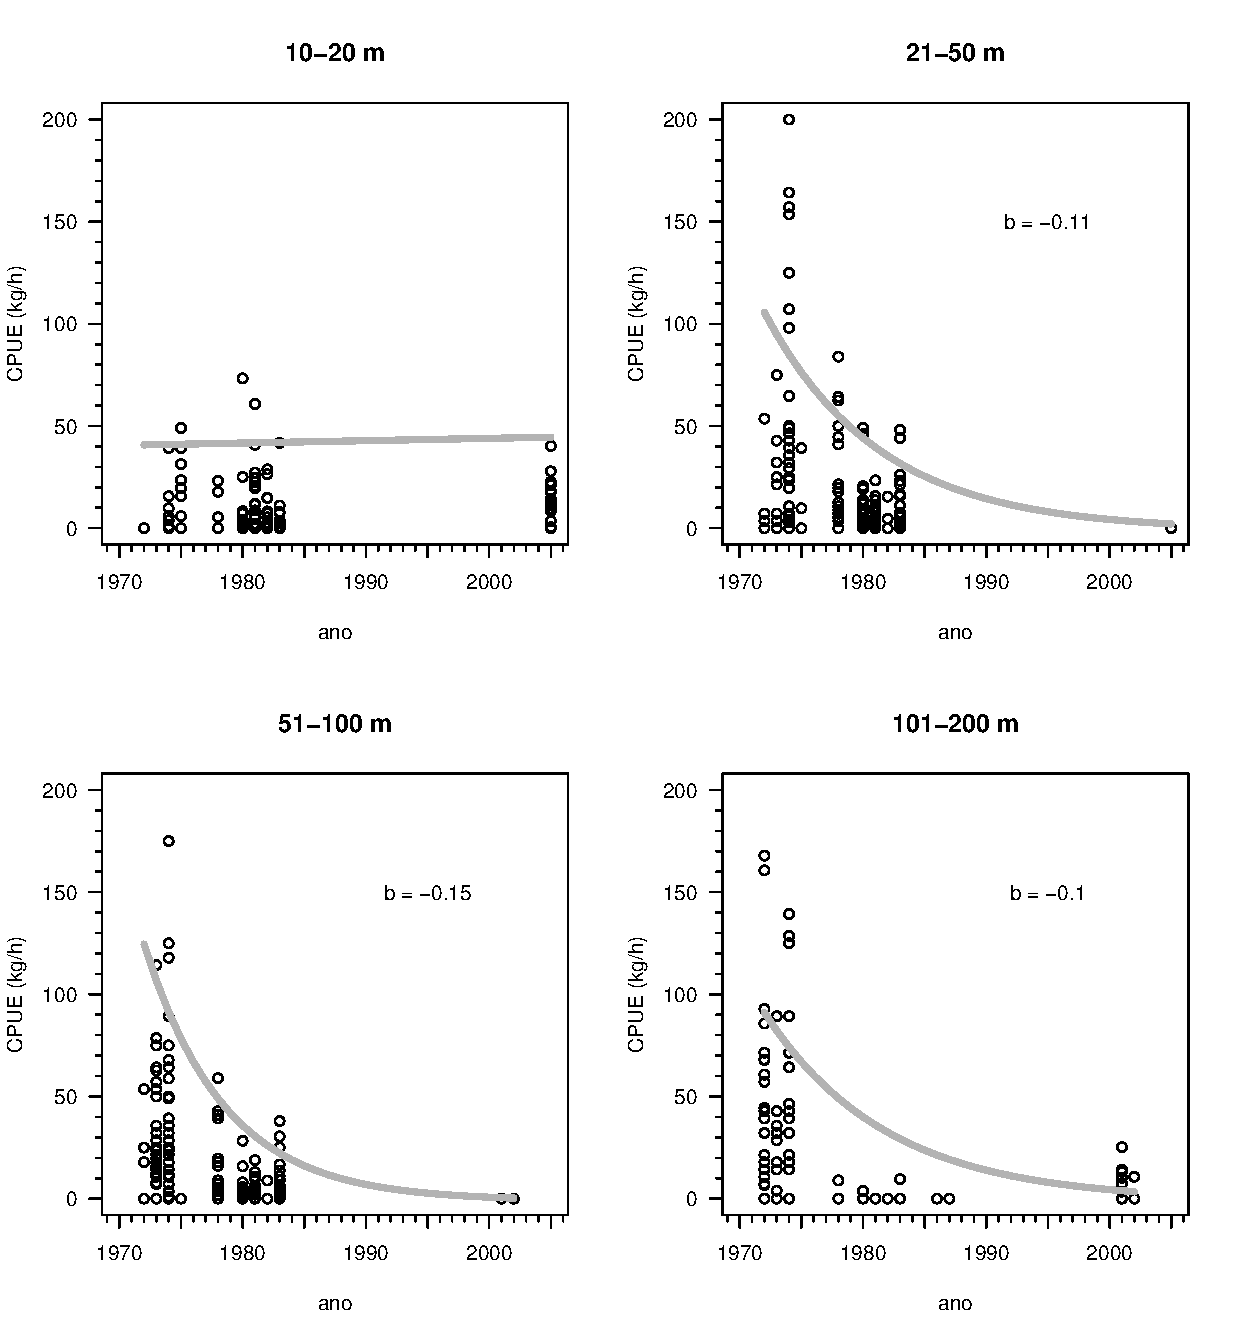
\includegraphics[width=\textwidth]{VIOLA_CPUEXPROFDECADAS}
\end{center}
\caption[Variação temporal da Captura por Unidade de Esforço em kg/hora de arrasto de fundo, 
	 da viola \emph{Rhinobatos horkelii} por faixa de profundidade da Plataforma Sul]
	{A variação temporal da  Captura por Unidade de Esforço (CPUE) em kg/hora, 
	 da viola \emph{Rhinobatos horkelii} por faixa de profundidade da Plataforma Sul. 
	 Cada ponto é a CPUE de uma estação de arrasto de fundo em levantamentos 
	 nos anos 1972-2005. As linhas de tendência são ajustadas aos valores 
	 da CPUE máxima de cada ano ($CPUE_{t} = CPUE_{0} \times e^{bt}$).}
\label{fig:viola-cpue-porano-dadospreteritos}
\end{figure}

%%%

O conjunto de fatores constituído pela conformação física da Plataforma Sul, pelas condições 
oceanográficas, e pelo clima da região, resulta na existência de uma extensa área 
costeira rasa, com fundo plano de sedimento fino, com elevada produtividade biológica, e onde 
no verão a temperatura da água sobe até cerca de 24°C. Com isto existe ao longo da costa um 
excelente berçário para a viola e uma ampla área do hábitat adequado para as atividades 
reprodutivas dos adultos de ambos os sexos durante o verão. Ao mesmo tempo a plataforma 
continental é larga e oferece condições favoráveis para a vida dos adultos durante as outras 
estações do ano. As condições ecológicas da Plataforma Sul  possibilitam uma elevada
abundância de \emph{R. horkelii}. 
% Em comparação com dados estatísticos da FAO sobre a pesca em 
% outras regiões do mundo, a pescaria da viola no Rio Grande do Sul na década de 1980 foi 
% a maior pescaria jamais registrada de uma espécie de \emph{Rhinobatos}.  

A Plataforma Sul  é a região mais importante da área de distribuição geográfica da viola 
como espécie. Pelo fato de que a população da viola nessa área ficou reduzida com mais 
de 80\% da sua abundância original, \emph{Rhinobatos horkelii} consta desde o ano de 2000 
como ``criticamente em perigo'' segundo os critérios da IUCN \citep{lessa2000}. % (Lessa e Vooren, 2000). % referência link na IUCN
O status de conservação da viola justifica urgentes ações de conservação da espécie 
na Plataforma Sul. 

\section*{Diretrizes biológicas para a conservação da viola na \mbox{Plataforma Sul} }

Ao longo da costa da Plataforma Sul, todas as fêmeas prenhes e todos os machos adultos 
da viola estão de novembro a março presentes com alta densidade em uma área que está 
ao alcance da pesca com o arrastão de praia. Isto explica as elevadas capturas de viola 
obtidas nessa pescaria durante a década de 1980, e o grande impacto dessa pescaria artesanal 
sobre a população da viola nos meses de novembro a março. A pesca industrial com o arrasto 
de parelha opera na plataforma interna e tem seu pico de produção da viola também nos meses 
de novembro a março \citep{martins2003,miranda2003}. 
Essa pesca incide nos adultos da viola durante os meses em que esses peixes se concentram 
nas profundidades de menos de 20~m da plataforma interna (Figura~\ref{fig:viola-cpueportrimestre}). 
Embora a pesca industrial com redes de arrasto é proibida na zona dentro da distância 
de 3 milhas náuticas da costa do Rio Grande do Sul, essa pesca é praticada freqüentemente 
dentro dessa zona e assim intercepta a migração reprodutiva da viola e atua sobre as 
concentrações da espécie nas águas adjacentes ao berçário costeiro, ou até mesmo dentro 
do berçário. 

O colapso do estoque após 1986 coincidiu com o término de um período de elevadas 
e crescentes capturas anuais, desde níveis em torno de 1000~t nos anos de 1975 a 1979 
até o máximo de 1.804~t no ano de 1984, seguido pelo declínio até níveis em torno de 200~t 
que foram mantidos a partir do ano de 1992 (Figura~\ref{fig:viola-desembarques-1945a2002}). 
No período de 1975 a 1986 foram capturadas ao todo 12.910~t de viola \citep{miranda2003}. 
Com um peso modal adulto de 5~kg segundo \citet{lessa1982}, % tese Lessa
essa cifra corresponde à captura da ordem de 2,6 milhões de indivíduos adultos num 
período de 11 anos. Ao longo desse período a pesca industrial na plataforma interna  
com o arrasto de parelha e a pesca artesanal com o arrastão de praia no berçário contribuíram 
em conjunto com cerca de 85\% das capturas anuais. Com isto, essas pescarias em conjunto 
capturavam a cada ano em média cerca de 200.000 indivíduos das concentrações reprodutivas 
no berçário e nas águas adjacentes a este. Com uma razão sexual de 1/1,  a captura anual 
foi da ordem de 100.000 fêmeas prenhes, e isto durante 11 anos. Com uma ninhada média 
de 6 neonatos por fêmea,  a captura anual dessas fêmeas prenhas resultou na perda 
de 600.000 neonatos por ano, ou cerca de 6,7 milhões de neonatos em 11 anos de pesca, 
mais os neonatos que as fêmeas que foram capturadas teriam produzido no resto da sua vida. 
Essas cifras são evidência da ordem de magnitude do impacto da pesca  sobre a 
reprodução da viola. O declínio da população da viola após o ano de 1986 foi causado 
pela elevada mortandade das fêmeas reprodutoras, em decorrência da pesca artesanal 
com arrastão de praia e da pesca industrial com arrasto de parelha na plataforma interna. 
Essa mortandade resultou na sobrepesca de recrutamento. Pela grande redução do número 
de nascimentos, esse número se tornou pequeno demais para compensar as mortes na população. 
Em decorrência da pesca no berçário e nas águas adjacentes a este, a população da viola 
entrou em declínio até ficar após o ano de 1992 com cerca de 16\% da sua abundância do ano 
de 1986. O caso da viola do Rio Grande do Sul entrou na literatura internacional como um 
exemplo da maneira como a pesca em áreas críticas pode causar o rápido declínio de uma 
espécie de elasmobrânquio vivíparo com distribuição geográfica restrita \citep{camhi1998}. % (Camhi et al., 1998).  

No ano de 2002 a captura de viola pelas frotas de arrasto do Rio Grande do Sul 
e Santa Catarina, em conjunto, foi de 521~t \citep{univali2003,ceperg2003}. % 561~t 
Essa captura foi obtida de uma população que estava reduzida até cerca de 
16\% da sua abundância do período 1975--1986, e teve sobre essa população um impacto 
cerca de duas vezes maior que a captura de 1.804~t teve sobre a população de 1984. 
Capturas anuais podem ser pequenas e ao mesmo tempo constituir um grande impacto sobre 
a população remanescente da viola. A conservação da viola da Plataforma Sul 
será obtida somente com sua maior proteção possível da pesca, 
especialmente da pesca nas áreas críticas da espécie. Essas áreas críticas são as 
águas costeiras nas profundidades de menos de 20~m e a plataforma externa 
nas profundidades de 100 a 200~m. 

%%%%%%%%%%%%%%%%%%%%%%%%%%%%%%%%%%%%%%%%%%%%%%%%%%%%%%%%%%%%%%%%%%%%%%%%%%%%%%%%%%%%%%%%%%%%

\chapter[Biologia e status de conservação dos cações-anjo \newline
         \emph{Squatina guggenheim}, \emph{S. occulta} e \emph{S. argentina}]
        {Biologia e status de conservação dos cações-anjo \emph{Squatina guggenheim},
	 \emph{S. occulta} e \emph{S. argentina}}\label{chap:anjos}

% A biologia e o status de conservação do cação-anjo-espinhoso \emph{Squatina guggenheim},
% 	 do cação-anjo-de-asa-curta \emph{Squatina occulta} e do cação-anjo-de-asa-longa
% 	 \emph{Squatina argentina}

\chapterprecishere{Carolus Maria Vooren \\
                   Sandro Klippel}

\chapterprecistoc{\small C. M. Vooren e S. Klippel}

\makeevenhead{myheadings}{Vooren, C. M. e S. Klippel}{}{}
% \makeoddhead{myheadings}{}{}{Biologia e status de conservação dos cações-anjo  
%                              \emph{Squatina guggenheim}, \emph{S. occulta} e \emph{S. argentina}}
\makeoddhead{myheadings}{}{}{Biologia e status de conservação dos cações-anjo}

\newpage

\section*{Sistemática, distribuição geográfica e pescarias}

Os cações-anjo têm o corpo achatado (Figura~\ref{fig:anjos-3spp}). % foto das tres espécies
Eles possuem duas nadadeiras dorsais e a nadadeira caudal, mas não têm a nadadeira anal. 
As nadadeiras peitorais são grandes em proporção com o resto do corpo e estendem-se para 
frente e para trás aos lados da cabeça e do abdômen. Essas extensões da nadadeira peitoral 
não são fixas à cabeça nem ao abdômen, e as cinco fendas branquiais são situadas na face 
lateral da cabeça. Esses detalhes da morfologia determinam que os cações-anjo são 
classificados como tubarões. Os cações-anjo possuem a boca e as fossas nasais em posição 
terminal, isto é, situadas na extremidade anterior da cabeça e com suas aberturas viradas 
para frente, enquanto em todos os outros elasmobrânquios a boca e as fossas nasais são 
situadas na face ventral da cabeça, com suas aberturas viradas para baixo. 
Em sua morfologia e anatomia, os cações-anjo são tão diferentes dos demais elasmobrânquios, 
que foi necessário criar uma divisão taxonômica especialmente para eles:  
a ordem Squatiniformes, com a única família Squatinidae que por sua vez possui 
o único gênero \emph{Squatina} \citep{compagno2005}. % (Compagno, 2005). 

%
% FOTOGRAFIA COM AS 3 ESPÉCIES DE ANJO
%
%%%%%%%%%%%%%%%%%%%%%%%%%%%%%%%%%%%%%%%%%

\begin{figure}
\begin{center}
\includegraphics[height=0.8\textheight]{CACOES-ANJO}
\end{center}
\caption[As três espécies de cação-anjo da Plataforma Sul: 
	 \emph{Squatina guggenheim}, \emph{Squatina occulta} e 
	 \emph{Squatina argentina}]
	{As três espécies de cação-anjo da Plataforma Sul. 
	 De cima para baixo: (a) \emph{Squatina guggenheim}, (b) \emph{Squatina occulta} e 
	 (c) \emph{Squatina argentina}, segundo a nomenclatura proposta por \citet{vooren1991}.}  % Vooren e Silva (1991).}
\label{fig:anjos-3spp}
\end{figure}

%%%

Para as três espécies de cação-anjo da Plataforma Sul é aqui usada a nomenclatura 
científica proposta por \citet{vooren1991}, % Vooren e Silva (1991), 
a saber:  \emph{Squatina guggenheim} Marini, 1936, \emph{S. argentina} (Marini, 1930) 
e  \emph{Squatina occulta} Vooren e Silva 1991 (Figura~\ref{fig:anjos-3spp}). % foto das 3 espécies
Essa nomenclatura é usada pela IUCN nos diagnósticos do estado de 
conservação dos cações-anjo \citep{chiaramonte2004a,chiaramonte2004b}. % (Chiaramonte, 2000a, 2000b). 
Nos cações-anjo, abas da pele recobrem cada uma das duas fossas nasais e são denominadas 
de cortinas nasais.  A forma da cortina nasal varia entre espécies de \emph{Squatina} \citep{COMPAGNO1984A}. % (Compagno, 1984). 
Porém nas três espécies da Plataforma Sul a cortina nasal tem a mesma forma, sendo composta de 
três lóbulos com bordas lisas. Dois destes lóbulos são longos e estreitos, em forma de espátula, 
e entre estes existe o lóbulo mediano que é curto e largo. A pele do lado dorsal do corpo é marrom, 
e cada espécie possui um padrão distinto e simétrico de manchas claras e escuras, mas a 
aparência dessas manchas varia entre indivíduos por causa da expansão ou contração dos 
cromatóforos no momento da captura do indivíduo. As diferenças morfológicas entre as três 
espécies são pequenas e referem-se principalmente à conformação da nadadeira peitoral e 
à presença ou ausência de uma fileira de espinhos ou tubérculos entre a cabeça 
e a 1ª nadadeira dorsal (Tabela~\ref{tab:anjos-morfologia}). % caracteristicas morfologiacas das 3 espécies

%
% TABELA COM AS CARACTERISTICAS MORFOLOGICAS DOS ANJOS
%
%%%%%%%%%%%%%%%%%%%%%%%%%%%%%%%%%%%%%%%%%%%%%%%%%%%%%%%

\begin{table}
\caption[Características morfológicas dos cações-anjo \emph{Squatina guggenheim}, 
	 \emph{S. occulta} e \emph{S. argentina}]
        {Características morfológicas do cação-anjo-espinhoso \emph{Squatina guggenheim}, 
	 do cação-anjo-de-asa-curta \emph{S. occulta} e do 
	 cação-anjo-de-asa-longa \emph{S. argentina}, segundo \citet{vooren1991}. 
	 Em negrito, as características que justificam os nomes comuns aqui usados. }
\label{tab:anjos-morfologia}
\begin{small}
\begin{tabularx}{\textwidth}{XXXX}
\toprule
					& \emph{S. guggenheim} & \emph{S. occulta} & \emph{S. argentina} \\ 
					& Marini, 1936		     & Vooren e Silva, 1991    & (Marini, 1930) \\
\midrule
\addlinespace
Fileira de espinhos ou tubérculos 
entre a cabeça e a 1a nadadeira dorsal
					& \textbf{Presente, mais nítido 
					nos juvenis e nos 
					machos}			& Ausente		& Ausente \\
\midrule
\addlinespace
Margem anterior externa da 
nadadeira peitoral			& Reta ou levemente 
					convexa.		& Reta ou levemente 
								convexa.		& Nitidamente convexa, 
											formando um ``ombro'' 
											ao lado da cabeça.  \\
\midrule
\addlinespace
Distância entre o ângulo anterior 
e o ângulo posterior da 
nadadeira peitoral 			& 30 a 32\% do CT	& \textbf{31 a 34\% do CT}	& \textbf{35 a 38\% do CT} \\
\midrule
\addlinespace
Extremidade posterior da nadadeira 
peitoral				& Não alcança o nível 
					do ângulo externo da 
					nadadeira pélvica.	& \textbf{Não alcança o nível 
								do ângulo externo da 
								nadadeira pélvica}	& \textbf{Alcança o nível do 
											ângulo externo da 
											nadadeira pélvica} \\
\midrule
\addlinespace
Fórmula dentária mais freqüente		& 10-10/10-10 a 
					11-11/11-11		& 9-9/10-10 a 
								10-10/11-11		& 12-12/12-12 a 
											12-12/13-13 \\
\bottomrule
\end{tabularx}
\end{small}
\end{table}

%%%

As diferenças entre as três espécies são grandes nos tamanhos do neonato e do adulto (Tabela~\ref{tab:anjos-parpopulacionais}) % parametros populacionais
e permitem reconhecer populações dessas espécies. Nos elasmobrânquios, o indivíduo é classificado 
como adulto a partir do momento da sua primeira maturação sexual, quando ele se torna apto para 
a reprodução pela primeira vez na vida. Em cada indivíduo adulto, características da maturidade 
sexual se manifestam em todos os momentos do ano. Nos cações-anjo o critério principal para 
classificar a fêmea como adulta é a gravidez e/ou a presença de folículos de cor amarelo-ouro 
no ovário, enquanto no macho adulto o clasper é rígido, grosso e longo, com sua ponta ultrapassando 
a ponta posterior da nadadeira pélvica. Perto da margem anterior do lado dorsal da nadadeira peitoral, 
o macho adulto dos cações-anjo possui fileiras de espinhos alares.

%
% TABELA COM OS PARAMETROS POPULACIONAIS DO ANJOS
%
%%%%%%%%%%%%%%%%%%%%%%%%%%%%%%%%%%%%%%%%%%%%%%%%%%%%%%%

\begin{table}
\caption[Características populacionais dos cações-anjo \emph{Squatina guggenheim}, 
	 \emph{S. occulta} e \emph{S. argentina}]
        {Características populacionais de \emph{S. argentina} (Marini, 1930),  
	 \emph{S. guggenheim} Marini, 1936   e  \emph{S. occulta} Vooren e Silva, 1991 
	 no sul do Brasil. CT = comprimento total. PT = peso total. 
	 L$\infty$, K e t$_{0}$ são 
	 os parâmetros da curva de crescimento segundo Von Bertalanffy. 
	 Os valores desses parâmetros são para ambos os sexos.    
	 Fontes: \citet{vooren1991,silva1996,vieira1996}.} % Vooren e Silva (1991), Silva (1996) e Vieira (1996).  }
\label{tab:anjos-parpopulacionais}
\begin{small}
\begin{tabularx}{\textwidth}{XXXX}
\toprule
		& \emph{S. guggenheim}		& \emph{S. occulta}		& \emph{S. argentina} \\
\midrule
\addlinespace
CT máximo	& 92~cm				& 131~cm			& 138~cm \\
\addlinespace
PT máximo	& 5~kg				& 18~kg				& 25~kg \\
\addlinespace
Idade máxima	& 12~anos			& 21~anos			& - \\
\addlinespace
CT na 1ª 
maturação 
sexual		& 72~cm				& 110~cm			& 120~cm \\
\addlinespace
PT na 1ª 
maturação 
sexual		& 2,6~kg			& 11,7~kg			& 14,6~kg \\
\addlinespace
Idade na 
1ª maturação 
sexual 		& 4~anos 			& 10~anos			& - \\
\addlinespace
CT ao nascer	& 25~cm				& 30~cm				& - \\
\addlinespace
PT ao nascer	& 120~g				& 300~g				& - \\
\addlinespace
Número de 
filhotes por 
gestação e 
número de 
ovócitos 
maduros no 
ovário		& 3--9, mais freqüente 5 e 6, 
		sem relação com o CT da 
		fêmea				& 4--10, mais freqüente 6 a 8, 
						sem relação com o CT da fêmea	& 7--11, mais freqüente 9 e 10, 
										sem relação com o CT da fêmea \\
\addlinespace
Número de 
ovários 	& Um ovário no lado esquerdo 
		da cavidade abdominal		& Um ovário no lado esquerdo da 
						cavidade abdominal		& Dois ovários simetricamente 
										dispostos \\
\addlinespace
Diâmetro e 
peso do 
folículo 
ovariano 
maduro		& 5~cm e 50~g			& 7~cm e 150~g			& 7~cm e 150~g \\
\addlinespace
Peso médio 
do ovário
maduro 
		& 300~g				& 1000~g			& 1300~g (os dois ovários juntos) \\
\addlinespace
L$\infty$	& 94,7~cm			& 138,9~cm			& - \\
\addlinespace
K		& 0,275				& 0,129				& - \\
\addlinespace 
t$_{0}$		& -1,145 anos			& -1,937 anos			& - \\
\bottomrule
\end{tabularx}
\end{small}
\end{table}

\emph{Squatina argentina}, \emph{S. guggenheim} e \emph{S. occulta} ocorrem somente na região sudoeste do Oceano Atlântico. 
No Brasil, essas três espécies ocorrem desde o Rio de Janeiro até a latitude de 34°S na fronteira 
marítima com Uruguai \citep{soto2001a}. % (Soto, 2001). 
No Uruguai, \emph{S. occulta}, \emph{S. argentina} e \emph{S. guggenheim} são capturados 
pela pesca com arrasto de fundo na plataforma interna \citep{meneses2003,paesch2003}. % (Meneses e Paesch, 2003; Paesch e Domingo, 2003). 
Na Argentina, \emph{S. argentina} e \emph{S. guggenheim} ocorrem na latitude de 39°S 
da costa sul da Província de Buenos Aires \citep{marini1930,marini1936}. % (Marini, 1930; Marini, 1933). 
Segundo \citet{menni1984}, % Menni et al. (1984), 
\emph{S. argentina} é uma espécie rara na Argentina, e a 
\emph{Squatina} comum da costa bonaerense possui uma fileira mediana dorsal de espinhos conspícuos. 
Segundo \citet{cousseau2000}, % Cousseau e Perrotta (1998), 
esta forma de \emph{Squatina} se distribui até a latitude 
de 45°S e alcança CT de 130~cm. Com isto, a \emph{Squatina} bonaerense possui características de duas 
espécies brasileiras: o CT máximo de \emph{S. occulta} e os espinhos dorsais de \emph{S. guggenheim}. 

Nas estatísticas da pesca do Brasil, as espécies de \emph{Squatina} são agrupadas na categoria ``cação-anjo''.  
Nos anos de 1983 a 1993, a captura anual de cação-anjo na plataforma do Rio Grande do Sul pela frota 
de Rio Grande variou entre 1.051 e 2.296~t, constituída de  \emph{S. guggenheim} e \emph{S. occulta} \citep{miranda2003}. % (Miranda e Vooren, 2003).  
No Uruguai, as capturas anuais de \emph{S. argentina}, \emph{S. guggenheim} e \emph{S. occulta} em conjunto
foram de cerca de 300~t nos anos 1998--2001 \citep{paesch2003}. % (Paesch e Domingo, 2003). 
Na Argentina as capturas anuais de cações-anjo foram de cerca de 4.000 toneladas nos anos 1992--1998,
mas com o declínio de 58\% da CPUE da frota costeira de arrasto de fundo \citep{massa2003}. % (Massa e Hozbor, 2003).
Além das pescarias de cações-anjo no Atlântico Sudoeste, a única outra importante pescaria de cações-anjo de que 
se tem registro foi aquela de  \emph{S. californica} na costa oeste dos EUA. Essa pescaria teve seu pico com a 
captura de 563~t no ano de 1986 \citep{bonfil1994}. % (Bonfil, 1994). 

\section*{Hábitat, alimentação e modo de vida dos cações-anjo}

Os cações-anjo vivem em fundos de areia ou lama da plataforma continental e do talude, 
desde águas costeiras rasas até a profundidade de 1300~m. Os cações-anjo se alimentam 
principalmente de peixes, crustáceos e  cefalópodes. Enterrado e imóvel na camada superficial 
do sedimento, o cação-anjo aguarda, e com um rápido movimento da cabeça agarra com os dentes 
uma presa que se aproxima até o alcance do bote \citep{bigelow1948,COMPAGNO1984A}. % (Bigelow e Schroeder 1948, Compagno 1984). 
Seu método de caça é determinado pela posição terminal da  sua boca, que faz com que o 
cação-anjo morda para cima quando levanta a cabeça, e pela sua dentição. 
Seus dentes são pequenos e pontiagudos, de tamanho e formato uniformes, e dispostos em três séries, 
com cerca de 20 dentes em cada série em ambas as maxilas. Com isto, o cação-anjo possui 
cerca de 120 dentes funcionais na boca. Esta dentição é do 
tipo ``de agarrar'' segundo a classificação de \citet{cappetta1986}, % Cappetta (1986), 
e determina que o cação-anjo segura a presa eficientemente mas não a mastiga nem 
a corta com os dentes. O cação-anjo seleciona presas de tamanho adequado para serem engolidas 
por inteiro. Moluscos bivalves e gastrópodes também constam como itens alimentares dos cações-anjo, 
e existe um registro de um cação-anjo agarrando na superfície do mar uma ave 
marinha da família dos biguás \citep{bigelow1948,COMPAGNO1984A}. % (Bigelow e Schroeder, 1948; Compagno, 1984). 
Fora o método de emboscada para a captura de presas que nadam perto do fundo do mar, 
o cação-anjo possui métodos alternativos para caçar suas presas. 

Na natação, os cações-anjo obtêm propulsão somente pelos movimentos da cauda, 
como fazem os tubarões em geral \citep{bigelow1948}. % (Bigelow e Schroeder 1948). 
O cação-anjo se apóia nas suas nadadeiras peitorais quando ele dá o bote para 
cima para agarrar uma presa, mas ele não as usa  para propulsão.  Em fotografias é observado 
que o cação-anjo ajusta a posição dessas nadadeiras para 
assim controlar a direção do seu nadar \citep{server1989}. % (Server 1989). 
A nadadeira caudal é pequena, ao passo que o corpo como um todo é grande e pesado, 
com densidade específica tal que dentro d'água, o peso de um cação-anjo é cerca de 
duas vezes aquele de um tubarão pelágico com o mesmo volume corporal \citep{stevens1987}. % (Stevens, 1987). 
Essa conformação do corpo determina que o cação-anjo nada lentamente. 
Isto foi confirmado no mar da Califórnia mediante o rastreamento de nove espécimes 
adultos de \emph{S. californica}  munidos de transmissores de ultra-som \citep{standora1977}. % (Standora e Nelson, 1977). 
Durante o dia esses peixes foram pouco ativos, com deslocamento médio de cerca de 50~m em uma hora, 
e com pouco ou nenhum deslocamento em torno do meio-dia. Durante a noite eles nadaram muito, 
sempre perto do fundo, com velocidades de 0,5 a 1,8~km/h, e ocasionalmente com breves 
arrancadas de cerca de 3~km/h, que foi a velocidade máxima observada. 
O percurso noturno foi de 2 a 9~km e com muitas curvas, sempre dentro de uma mesma área 
de aproximadamente 1,5~km\textsuperscript{2}. O cação-anjo é um animal solitário e sedentário que possui 
no fundo do mar um território dentro do qual ele se desloca vagarosamente durante a noite 
e onde ele  permanece parado durante o dia, esperando que uma presa se aproxime a ele. 
Seu estilo de vida é simples, devagar e de baixo consumo de energia. Talvez isto explica 
como os cações-anjo foram capazes de sobreviver desde 
o período Jurássico até hoje \citep{cappetta1987}. % (Cappetta, 1987).  

A atividade noturna dos cações-anjo determina que durante a noite esses peixes são 
vulneráveis à pesca com redes de emalhe colocadas no fundo do mar. Isto explica o 
grande sucesso da pesca com redes de emalhe, quando essa arte de pesca foi introduzida 
no hábitat dos cações-anjo da Plataforma Sul na década de 1990. Em média a captura de 
cações-anjo em uma viagem de pesca com essas redes de emalhe foi seis vezes maior que 
a captura desses peixes em uma viagem de pesca com redes de arrasto simples 
no mesmo período \citep{miranda2003}. % (Miranda e Vooren, 2003). 

No crânio dos peixes existem os dois labirintos, que contêm os órgãos da audição e do equilíbrio. 
Em quase todos os elasmobrânquios, os labirintos contêm massas brancas e pastosas, que são 
aglomerados de partículas de carbonato de cálcio dentro de uma matriz de gelatina. 
Essas partículas, denominadas de otocónios, são produzidas pelo labirinto, e os aglomerados 
de otocónios têm as mesmas funções e as mesmas posições no labirinto, como os otólitos 
dos peixes ósseos. Porém nos cações-anjo os otocónios são pequenos grãos de mineral
oriundos do sedimento do fundo do mar, e que entram no labirinto 
através do  ducto endolinfático que conecta o labirinto com a superfície dorsal da cabeça. 
Os cações-anjo possuem ``otólitos exógenos'' \citep{daniel1922}. % (Daniel, 1922). 

Nos elasmobrânquios vivíparos, normalmente o útero permanece fechado durante a gestação, 
pela ação da musculatura lisa do colo do útero na  junção deste com a cloaca. Nos cações-anjo 
no entanto, após a fase inicial da gestação o colo do útero se abre e a cloaca se distende, 
de modo que os dois úteros e a cloaca em conjunto formam um único espaço em forma de coração, 
denominado de ``câmara útero-cloacal'', dentro da qual os embriões completam seu desenvolvimento 
até nascerem (Figura~\ref{fig:anjos-camara-utero-cloacal}). % fotos camara uterlo-cloacal
Os cações-anjo possuem a ``gestação cloacal''.  A cloaca permanece aberta ao ambiente externo, 
de modo que os embriões se desenvolvem na água do mar que entra na cloaca \citep{sunye1997}. % (Sunyé e Vooren, 1997).  
Isto explica porque a fêmea grávida dos cações-anjo aborta facilmente quando ela é pescada (Figura~\ref{fig:anjos-camara-utero-cloacal}). % fotos camara uterlo-cloacal
Os embriões na câmara útero-cloacal já constroem seus otólitos exógenos \citep{miranda1998}. % (Miranda, 2000). 
Os embriões aproveitam grãos de sedimento que entram na cloaca com a água do mar, e assim os 
filhotes nascem com seus otólitos plenamente formados. 

%
% FOTOGRAFIA COM A CAMERA UTERO-CLOACAL
%
%%%%%%%%%%%%%%%%%%%%%%%%%%%%%%%%%%%%%%%%%

\begin{figure}
\begin{center}
\includegraphics[height=0.7\textheight]{ANJO-UTERO}
\end{center}
\caption[Câmara útero-cloacal de \emph{Squatina guggenheim}]
	{A gestação de \emph{Squatina guggenheim}, com nas fotos (a) e (b) a cavidade abdominal 
	 com os órgãos reprodutivos em vista ventral, com o lado cranial para cima. 
	 (a) A câmara útero-cloacal  inteira; o perfil dos embriões aparece na foto. 
	 (b) A câmara útero-cloacal aberta, mostrando-se os embriões. 
	 (c) Uma fêmea grávida foi capturada com o arrasto de fundo e abortou seus embriões. 
	 A câmara útero-cloacal é constituída pelo útero direito UD, o útero esquerdo UE 
	 e a cloaca CL. SV = saco vitelínico do embrião. OV = ovário.}
\label{fig:anjos-camara-utero-cloacal}
\end{figure}

%%%

A maneira como os cações-anjo diferem dos demais elasmobrânquios na forma do seu corpo, 
no seu modo de vida e na sua biologia, é talvez relacionada com o fato de que os cações-anjo 
são um grupo extremamente antigo. Cações-anjo exatamente como os de hoje existiram 
no período Jurássico \citep{cappetta1987}. % (Cappetta, 1987).
Entre os elasmobrânquios atuais, os cações-anjo são um dos poucos grupos com idade paleontológica 
de mais de 120 milhões de anos. Isto confere ao cação-anjo o status de um sobrevivente que 
atravessou o tempo, como uma relíquia da evolução da vida. Esses aspectos determinam o valor 
intrínseco dos cações-anjo e são motivos para a proteção desses animais.  

\section*{A reprodução dos cações-anjo e o impacto da pesca sobre as populações dos cações-anjo}

Os cações-anjo se reproduzem pela viviparidade lecitotrófica. O ovócito maduro  contém o vitelo 
necessário para o crescimento do futuro embrião. Durante a gestação o embrião absorve esse vitelo 
e assim se desenvolve até o nascer. Para cada gestação a fêmea de \emph{S. guggenheim} produz no seu 
ovário uma quantia de cerca de 300~g de vitelo, enquanto para \emph{S. occulta} 
essa quantia é de cerca de 1000~g (Figura~\ref{fig:anjos-ovario-occulta}, Tabela~\ref{tab:anjos-parpopulacionais}). % foto ovario de S. occulta e tabela c/ caracteristicas populacionais
Essa quantia de vitelo constitui cerca de 10\% do peso total da fêmea em ambas as espécies. 
Em concordância com o estilo de vida vagaroso dos cações-anjo, a formação dessa grande quantia 
de vitelo ocupa dois anos da vida da fêmea de \emph{S. guggenheim}. Em seguida a fêmea copula e engravida. 
A gestação tem duração de 12 meses. Com isto, o ciclo reprodutivo da fêmea de \emph{S. guggenheim} tem 
a duração de três anos: dois anos para a maturação dos ovócitos, e um ano para a gestação \citep{silva1996}. % (Silva 1996). 

%
% FOTOGRAFIA DO OVARIO DA SQUATINA OCCULTA
%
%%%%%%%%%%%%%%%%%%%%%%%%%%%%%%%%%%%%%%%%%%%%%%%%%%%%

\begin{figure}
\begin{center}
\includegraphics[width=\textwidth]{OVARIO-OCCULTA}
\end{center}
\caption[Ovário de \emph{Squatina occulta}]
	{Um ovário de \emph{Squatina occulta} com sete folículos contendo ovócitos maduros.}
\label{fig:anjos-ovario-occulta}
\end{figure}

%%%

Nos cações-anjo, a idade na primeira reprodução tem um valor médio que é atributo da população, 
mas essa idade varia entre indivíduos. Em decorrência disto existem a cada momento fêmeas 
adultas em diferentes fases do ciclo reprodutivo.  Embora a fêmea individual de \emph{S. guggenheim}
reproduz uma só vez a cada três anos, existem sempre fêmeas prenhes na população, e a cada ano 
um certo número de fêmeas dá à luz. Nos levantamentos com arrasto da Plataforma Sul na década de 
1980 foi observado que 30\% das fêmeas adultas de \emph{S. guggenheim} estavam prenhes, em concordância 
com o ciclo trienal dessa espécie.  Nesses levantamentos,  poucos neonatos de \emph{S. occulta} foram 
capturados, e apenas 22\% das fêmeas adultas de \emph{S. occulta} estavam prenhes \citep{silva1996}. % (Silva, 1996). 
Isto é indício de que o ciclo reprodutivo da fêmea de \emph{S. occulta} pode ter a duração de quatro 
ou cinco anos, talvez com variação entre indivíduos e entre ciclos sucessivos do mesmo indivíduo. 
Essa é a razão da baixa abundância dos neonatos de \emph{S. occulta}. 

Com o ciclo reprodutivo de três a cinco anos, e com as idades que constam na Tabela~\ref{tab:anjos-parpopulacionais}, 
calcula-se que a fêmea de \emph{S. guggenheim} e de \emph{S. occulta} reproduz no máximo quatro vezes em 
toda sua vida, assim produzindo cerca de 20 a 30 filhotes ao todo. Os cações-anjo reproduzem 
com baixa intensidade. Ao mesmo tempo os cações-anjo têm poucos inimigos naturais, de modo 
que sua pequena taxa de reprodução é o suficiente para compensar sua também pequena 
taxa de mortalidade.  Quando em determinada região existe uma abundante população de 
cações-anjo, essa população é o resultado de um longo e lento processo de crescimento 
populacional, com uma duração da ordem de séculos. Uma população de cações-anjo não é 
capaz de crescer mais do que lentamente. Portanto, uma pesca intensa causa o declínio 
dessa população. Um exemplo disto é o colapso da pescaria de \emph{S. californica} na costa 
oeste dos EUA após oito anos de pesca intensiva \citep{bonfil1994}. % (Bonfil, 1994). 

\section*{\emph{Squatina guggenheim}: a distribuição espacial, a migração das fêmeas prenhes, 
          o berçário costeiro, e o impacto da pesca na Plataforma Sul}

% fo profundidade
%
% HISTOGRAMA COM A OCORRÊNCIA DE S GUGGENHEIM POR PROFUNDIDADE
%
%%%%%%%%%%%%%%%%%%%%%%%%%%%%%%%%%%%%%%%%%%%%%%%%%%%%%%%%%%%%%%%

\begin{figure}
\begin{center}
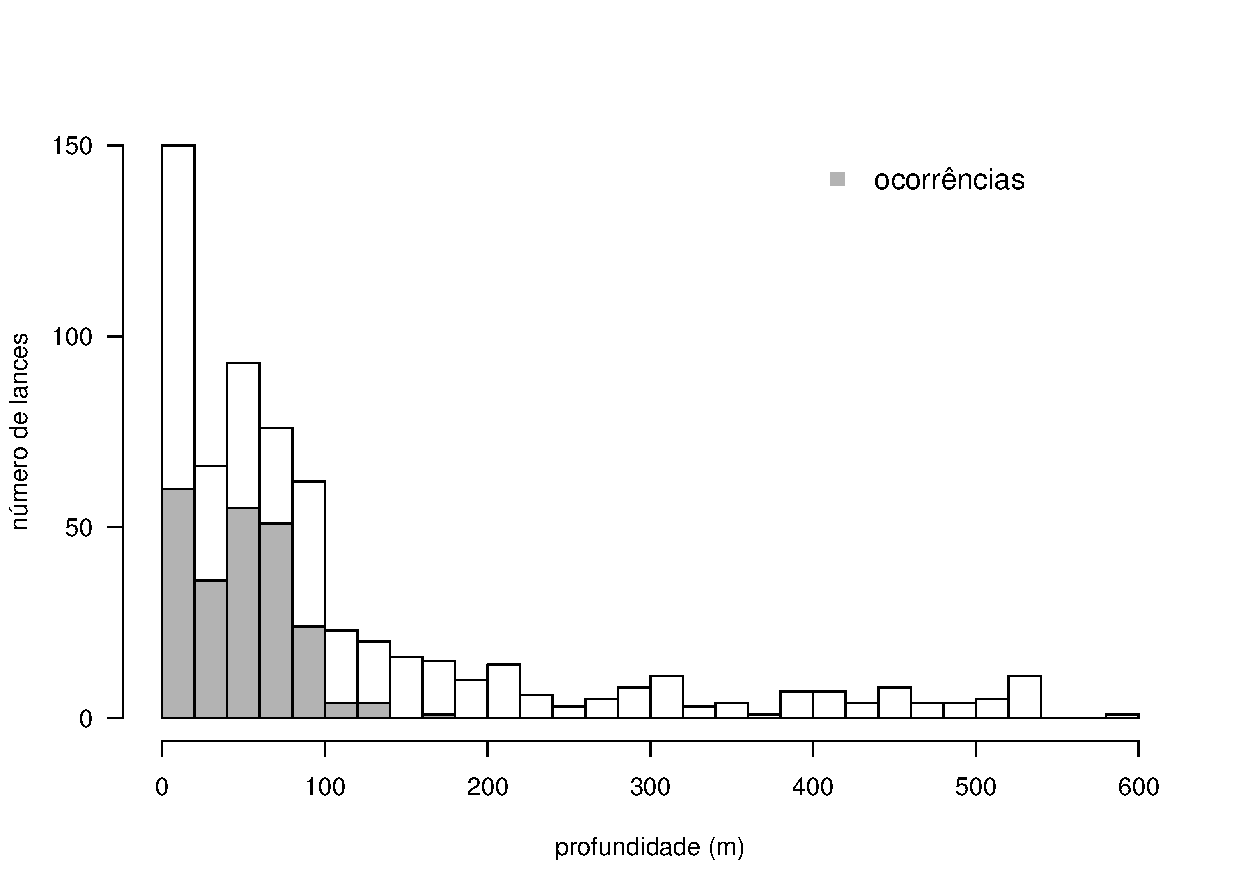
\includegraphics[width=\textwidth]{GUGGENHEIM_DISTRIBPROF}
\end{center}
\caption[A freqüência de ocorrência do cação-anjo-espinhoso \emph{Squatina guggenheim} 
	em relação com a profundidade, nas estações de arrasto de 
	fundo na Plataforma Sul nos anos 1980--2005]
	{A freqüência de ocorrência do cação-anjo-espinhoso \emph{Squatina guggenheim} 
	em relação com a profundidade, nas estações de arrasto de 
	fundo na Plataforma Sul nos anos 1980--2005. 
	As barras cheias denotam presença da espécie, 
	as barras vazias denotam sua ausência.}
\label{fig:fo-guggenheim-profundidade}
\end{figure}

%%%

% mapa cpue
%
% MAPAS COM DISTRIBUIÇÃO ESPACIAL DA CPUE DE S. GUGGENHEIM
%
%%%%%%%%%%%%%%%%%%%%%%%%%%%%%%%%%%%%%%%%%%%%%%%%%%%%%%%%%%%%%%%

\begin{figure}
\begin{center}
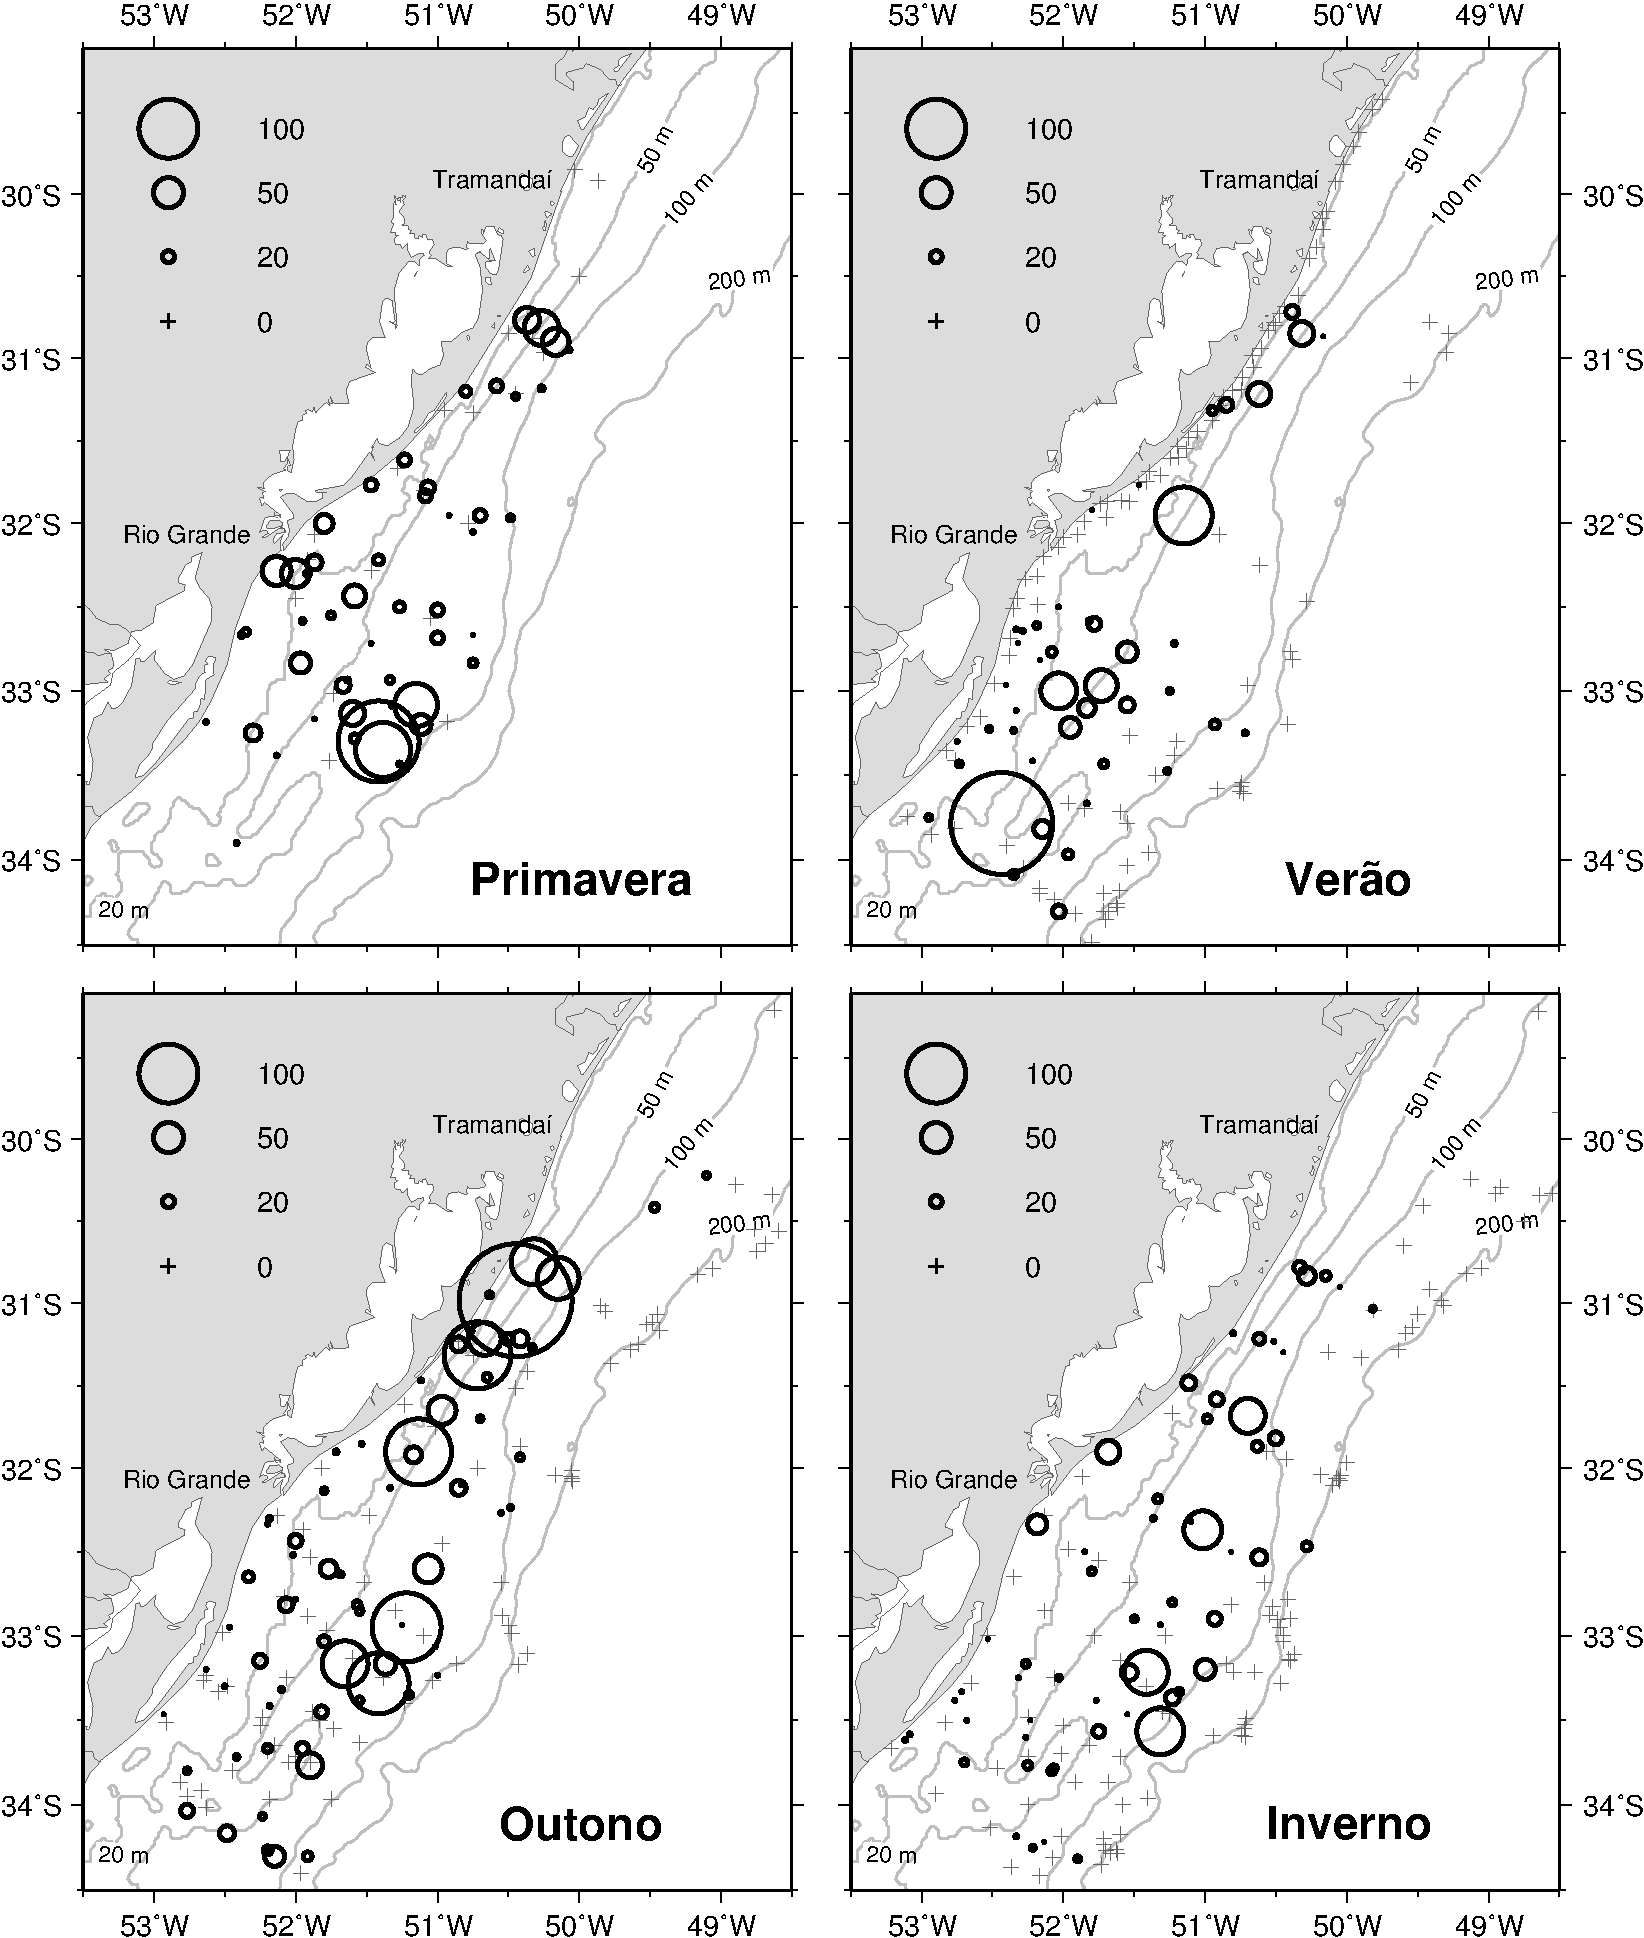
\includegraphics[width=\textwidth]{GUGGENHEIM_MAPA_DISTRIBUICAO_CPUE}
\end{center}
\caption[Variação sazonal da distribuição espacial da CPUE em kg/hora, do cação-anjo-espinhoso \emph{Squatina guggenheim}]
	{A variação sazonal da distribuição espacial da CPUE em kg/hora, do cação-anjo-espinhoso \emph{Squatina guggenheim} 
	 na Plataforma Sul, nos levantamentos com arrasto de fundo nos anos de 1980--2005. 
	 As cruzes indicam as posições das estações de arrasto de fundo sem captura da espécie.}
\label{fig:guggenheim-mapacpue}
\end{figure}

%%%
	  
Nos anos de 1980 a 1984, \emph{S. guggenheim} foi comum ao longo do ano na Plataforma Sul 
entre Solidão e Chuí, nas profundidades de 10 a 100~m (Figuras~\ref{fig:fo-guggenheim-profundidade}~e~\ref{fig:guggenheim-mapacpue}). % mapas cpue e FO por profundidade
Densidades maiores que 50~kg/h ocorreram durante o outono e inverno principalmente nas 
profundidades de  50 a 100~m, e durante a primavera e verão principalmente nas profundidades 
menores que 50~m, evidenciando-se uma migração sazonal para águas mais rasas na primavera-verão, 
e para águas mais profundas no outono-inverno (Figura~\ref{fig:guggenheim-cpueportrimestre}). % graficos CPUE x prof por epoca do ano
\citet{silva1996} observou que nas profundidades 
de 10 a 40~m, indivíduos juvenis e adultos de ambos os sexos são abundantes nos meses de novembro 
a fevereiro e escassos de agosto a setembro, enquanto o inverso ocorre nas profundidades 
de 60 a 100~m. Porém essa migração sazonal é realizada somente por uma parcela da população, 
porque a espécie permanece presente ao longo do ano em todas essas profundidades (Figuras~\ref{fig:guggenheim-mapacpue}~e~\ref{fig:guggenheim-cpueportrimestre}). 
A migração sazonal de somente uma parcela da população está relacionada com  o ciclo 
reprodutivo de \emph{S. guggenheim}. O parto dessa espécie ocorre de 
outubro a janeiro em águas costeiras \citep{silva1996}. % (Silva, 1996). 
O ciclo reprodutivo trienal da fêmea determina que na primavera e no verão 1/3 das fêmeas 
adultas estão prestes a parir e migram para a área do parto nas profundidades de menos de 40~m. 
Fêmeas adultas em outros estágios do ciclo reprodutivo, juvenis de ambos os sexos e machos adultos 
também aparecem nessas profundidades nos meses de novembro a fevereiro. Porém em 40 a 60~m, 
juvenis e adultos de ambos os sexos são abundantes durante o ano todo. Uma grande parte da população 
não se desloca sazonalmente entre profundidades. Por essa razão as amplitudes das temperaturas 
de verão e de inverno no hábitat da espécie se sobrepõem, com maior ocorrência da espécie 
em 16 a 19°C ao longo do ano (Figura~\ref{fig:guggenheim-distrib-tempfundo}). % FO por temperatura
As baixas temperaturas de inverno no hábitat  
da espécie refletem a influência do Corrente das Malvinas durante o inverno na plataforma 
ao sul da latitude de 32°S, onde uma parcela da população vive o ano todo (Figura~\ref{fig:guggenheim-mapacpue}). 
A elevada ocorrência da espécie em temperaturas de 21 a 25°C no verão reflete a migração 
de todas as fêmeas prenhes, e a dispersão de outros indivíduos da população, para as águas costeiras. 


%
% VARIAÇÃO SAZONAL DA CPUE (Kg/h)
%
%%%%%%%%%%%%%%%%%%%%%%%%%%%%%%%%%%%%%%%%%%%%%%%%%%%%%%%%%%%%%%%

\begin{figure}
\begin{center}
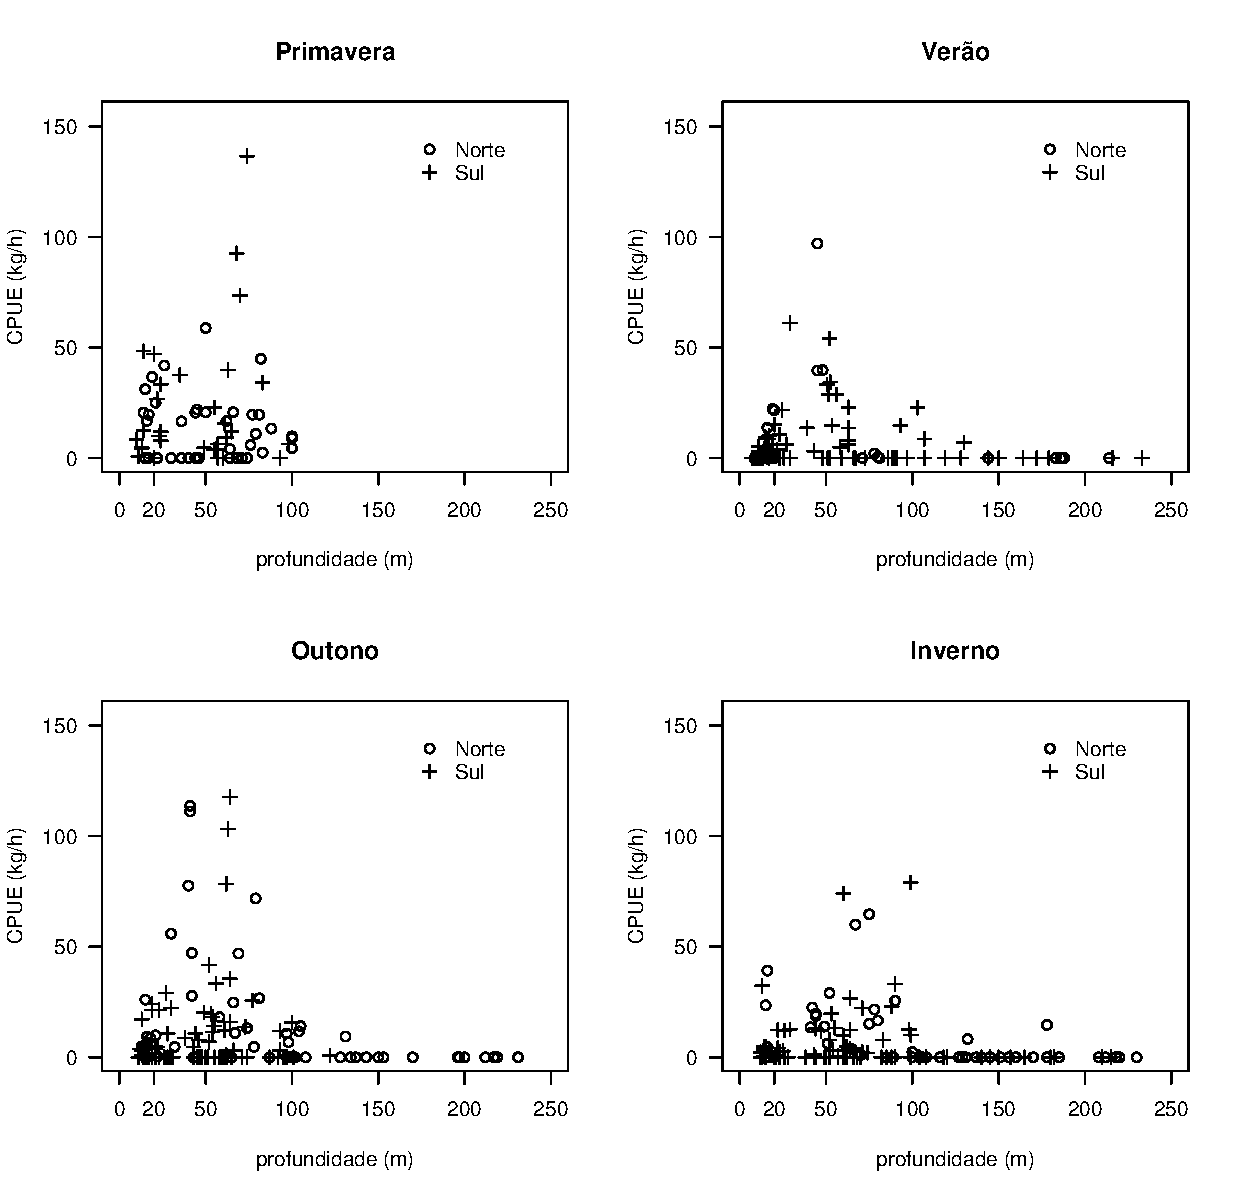
\includegraphics[width=\textwidth]{GUGGENHEIM_CPUEXPROFTRIMESTRES}
\end{center}
\caption[Variação sazonal da densidade populacional do cação-anjo-espinhoso \emph{Squatina guggenheim}]
	{A variação sazonal da densidade populacional do cação-anjo-espinhoso \emph{Squatina guggenheim} 
	 nas diferentes profundidades da Plataforma Sul, ao norte e ao sul de Rio Grande. 
	 Cada ponto é a Captura por Unidade de Esforço (CPUE) em kg/hora, de uma 
	 estação de pesca de arrasto de fundo nos anos de  1980--2005.}
\label{fig:guggenheim-cpueportrimestre}
\end{figure}

%%%

%
% FO DE S GUGGENHEIM POR TEMPERATURA DE FUNDO
%
%%%%%%%%%%%%%%%%%%%%%%%%%%%%%%%%%%%%%%%%%%%%%%%%%%%%%%%%%%%%%%%

\begin{figure}
\begin{center}
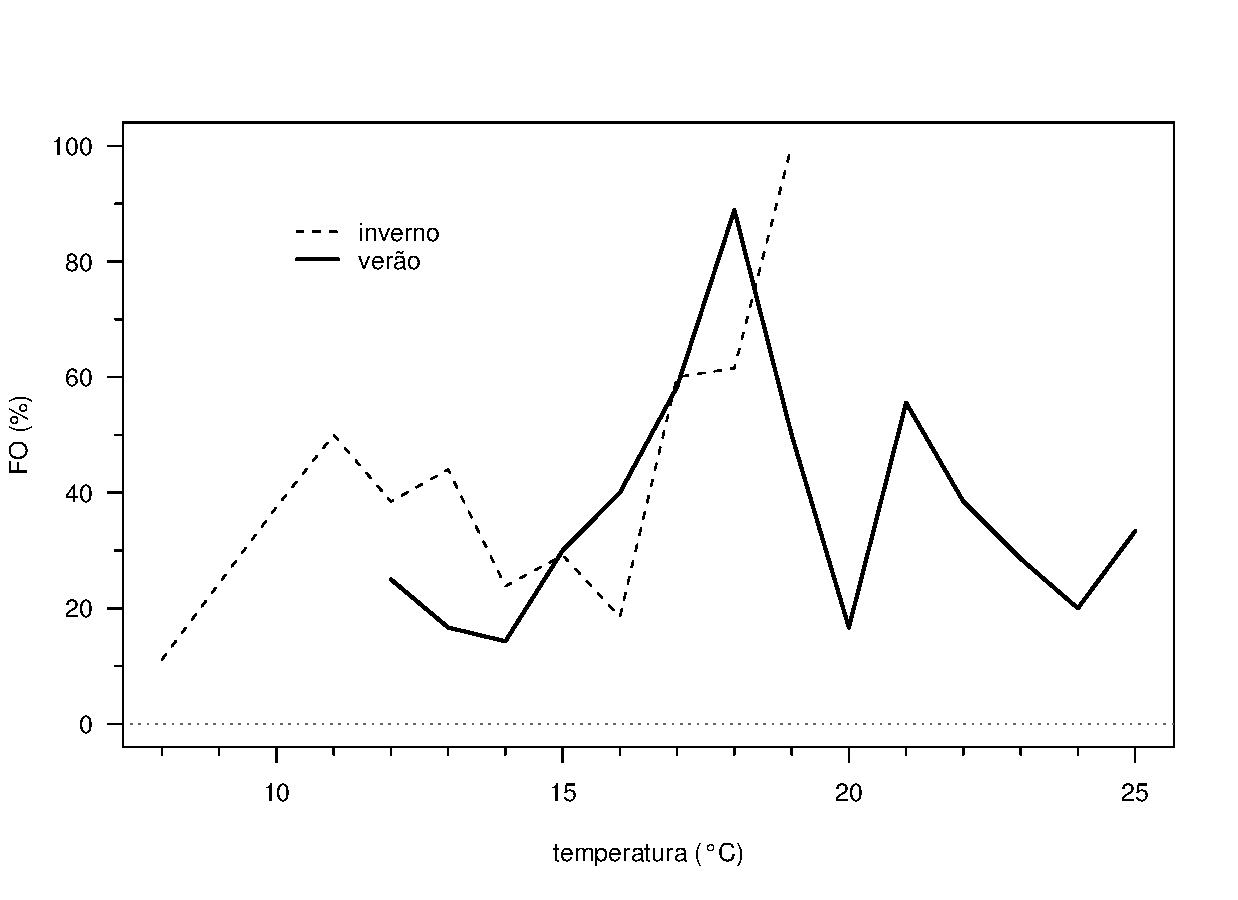
\includegraphics[width=\textwidth]{GUGGENHEIM_DISTRIBTEMPFUNDO}
\end{center}
\caption[Freqüência de ocorrência (FO) do cação-anjo-espinhoso \emph{Squatina guggenheim}
	 com relação à temperatura de fundo]
	{Freqüência de ocorrência (FO) do cação-anjo-espinhoso \emph{Squatina guggenheim}
	 com relação à temperatura de fundo, nos levantamentos com 
	 arrasto de fundo nos anos 1980--2005.}
\label{fig:guggenheim-distrib-tempfundo}
\end{figure}

%%%

\emph{S. guggenheim} nasce de outubro a fevereiro com CT de 24 a 28~cm, e alcança CT de cerca 
de 44~cm no final do primeiro ano de vida \citep{silva1996}. % (Silva, 1996). 
Neonatos são aqui definidos como indivíduos com  CT de 24 a 44~cm. 
Na década de 1980, neonatos e juvenis ocorreram nas águas 
rasas próximas à praia ao sul do Cassino (Figura~\ref{fig:guggenheim-distrib-arrasto1980}).  % distrib. comprimentos arrasto de praia anos 80
A área das profundidades de menos de 30~m entre as latitudes de 31°50'S e 33°30'S é o berçário 
de \emph{S. guggenheim}, onde ocorre o parto de outubro a fevereiro 
e onde os neonatos vivem durante o ano todo (Figura~\ref{fig:guggenheim-mapa-neonatos}). % mapa com localização de neonatos
Nos meses de outubro a fevereiro, todas as fêmeas prenhes atravessam a 
plataforma interna na sua migração para o berçário. As pescarias nas águas costeiras 
interceptam a migração reprodutiva das fêmeas prenhes e ao mesmo tempo capturam 
indivíduos de ambos os sexos em todas as fases da vida, desde neonatos a adultos, 
assim causando um impacto sobre o recrutamento da população de \emph{S. guggenheim}. 
Evidência desse impacto é a composição das capturas de \emph{S. guggenheim} da pesca 
em águas costeiras com redes de emalhe, arrasto de parelha e arrasto duplo. 
Ao mesmo tempo as pescarias nas profundidades de 50 a 100~m pelo arrasto simples
afetam a parcela da população de \emph{S. guggenheim} que se distribui sobre 
essa área durante o ano todo (Capítulo~\ref{chap:pesca-industrial}, Figura~\ref{fig:ct-gugenheim}).  % figura com CT por arte de pesca industrial

%
% DISTRIBUICAO DE COMPRIMENTOS GUGGENHEIM NA DECADA DE 1980
%
%%%%%%%%%%%%%%%%%%%%%%%%%%%%%%%%%%%%%%%%%%%%%%%%%%%%%%%%%%%%%%%

\begin{figure}
\begin{center}
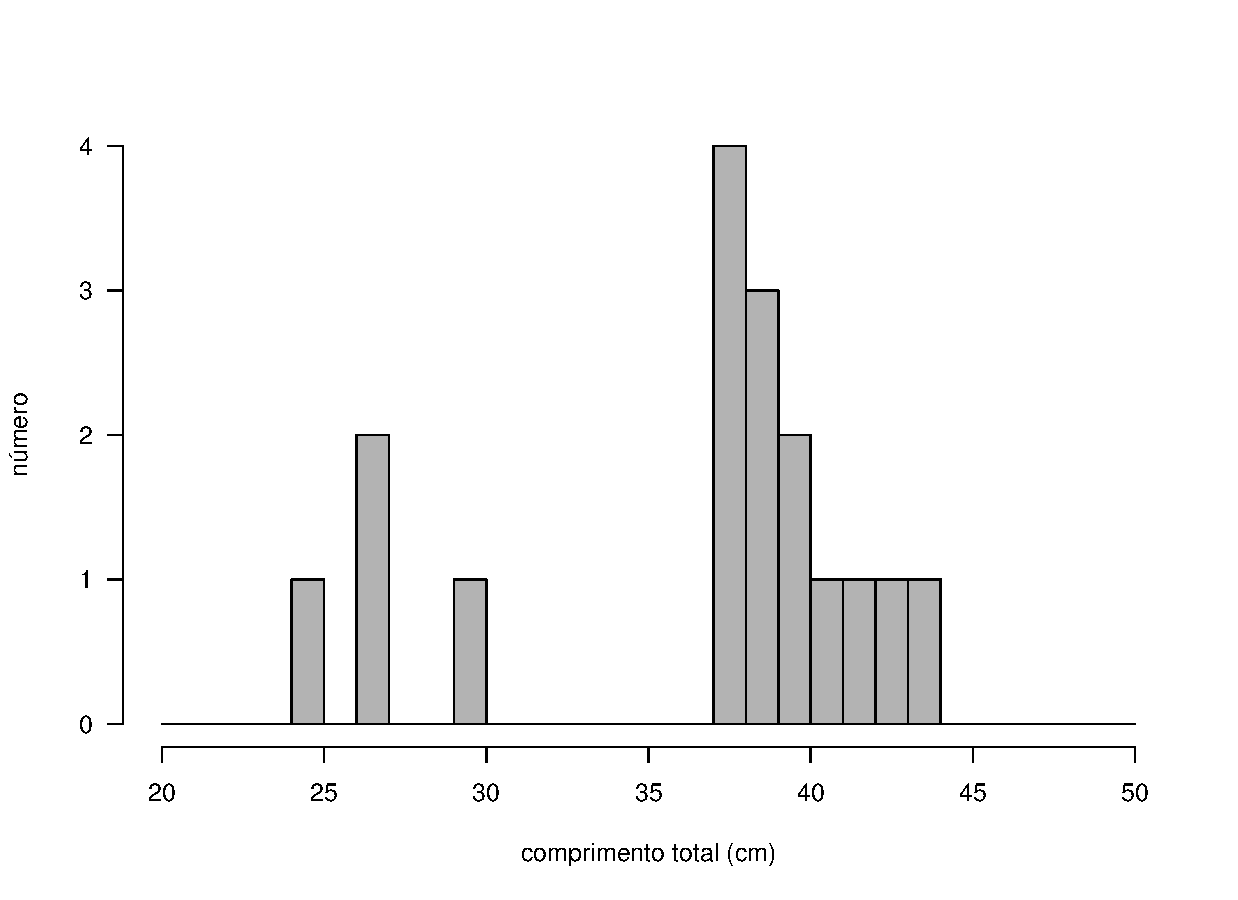
\includegraphics[width=\textwidth]{GUGGENHEIM_HISTOGRAMAPRAIA}
\end{center}
\caption[Composição de comprimento das capturas  do cação-anjo-espinhoso \emph{Squatina guggenheim} 
	 pela pesca artesanal com arrastão de praia]
	{Composição de comprimento das capturas  do cação-anjo-espinhoso \emph{Squatina guggenheim} 
	 pela pesca artesanal com arrastão de praia ao sul do Cassino nos anos 1980--1983.}
\label{fig:guggenheim-distrib-arrasto1980}
\end{figure}

%%%

%
% MAPA COM OCORRÊNCIAS DE NEONATOS
%
%%%%%%%%%%%%%%%%%%%%%%%%%%%%%%%%%%%%%

\begin{figure}
\begin{center}
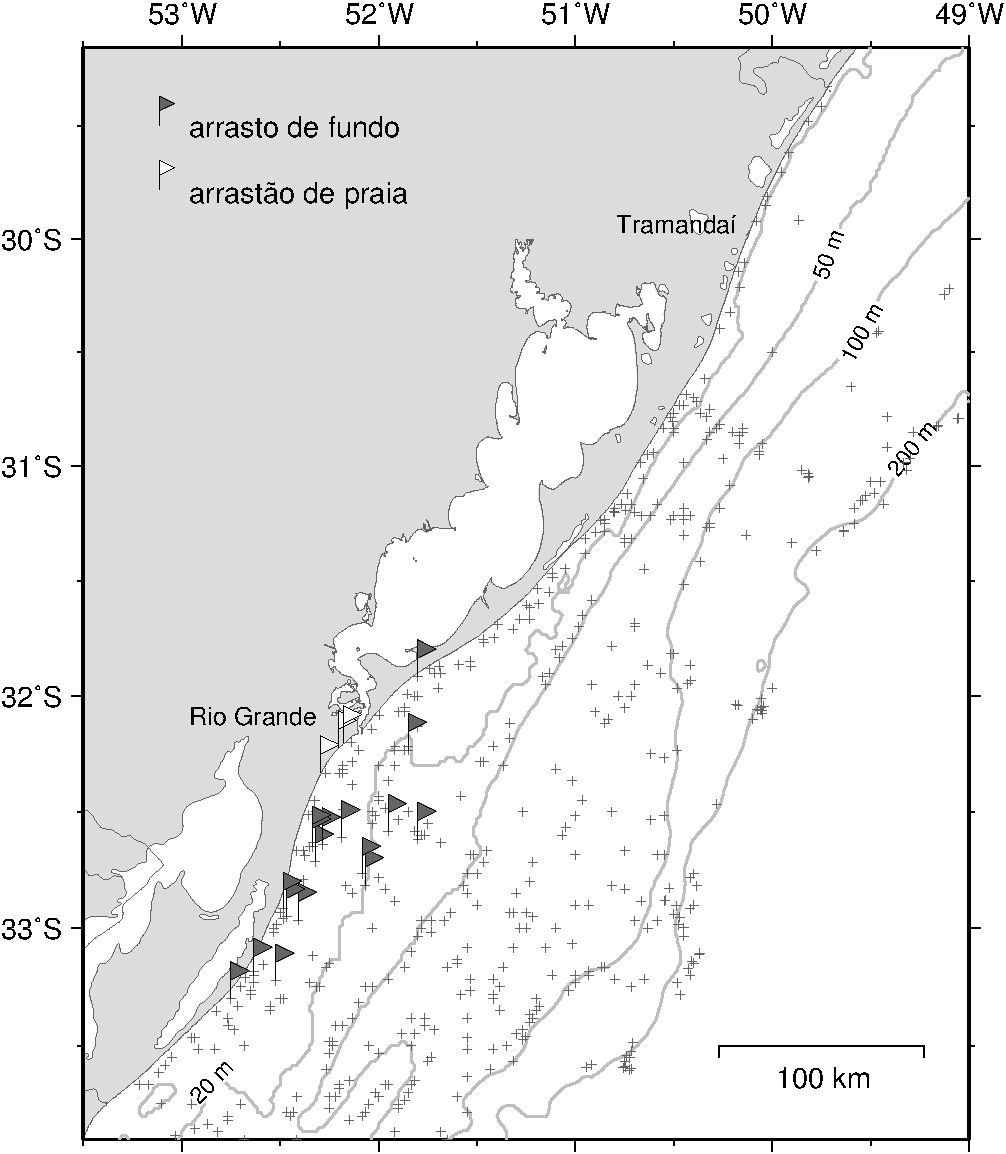
\includegraphics[width=\textwidth]{GUGGENHEIM_MAPA_NEONATOS}
\end{center}
\caption[Ocorrências de neonatos do cação-anjo-espinhoso \emph{Squatina guggenheim} na Plataforma Sul]
	{Ocorrências de neonatos do cação-anjo-espinhoso \emph{Squatina guggenheim} na Plataforma Sul, 
	 nas estações de pesca com arrasto de fundo do Cruzeiro SALVAR em 2005 e 
	 dos levantamentos pretéritos em 1980--1984, e nas capturas da pesca artesanal 
	 com arrastão de praia nos anos 1979--1981.}
\label{fig:guggenheim-mapa-neonatos}
\end{figure}

%%%

\section*{\emph{Squatina occulta}: a distribuição espacial, o berçário na plataforma externa, 
          e o impacto da pesca na Plataforma Sul }

%
% HISTOGRAMA COM A OCORRÊNCIA DE S OCCULTA POR PROFUNDIDADE
%
%%%%%%%%%%%%%%%%%%%%%%%%%%%%%%%%%%%%%%%%%%%%%%%%%%%%%%%%%%%%%%%

\begin{figure}
\begin{center}
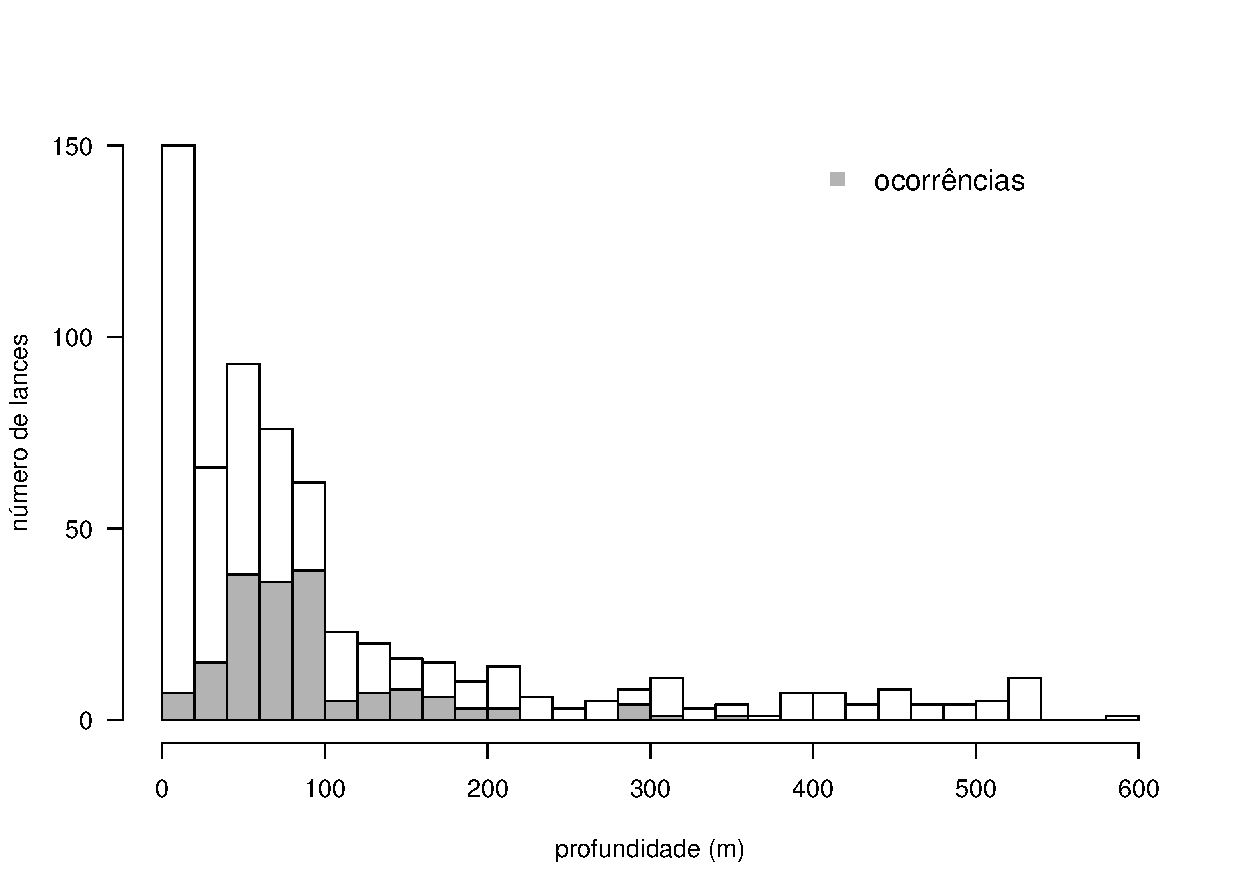
\includegraphics[width=\textwidth]{OCCULTA_DISTRIBPROF}
\end{center}
\caption[A freqüência de ocorrência do cação-anjo-de-asa-curta \emph{Squatina occulta} 
	em relação com a profundidade, nas estações de arrasto de 
	fundo na Plataforma Sul nos anos 1980--2005]
	{A freqüência de ocorrência do cação-anjo-de-asa-curta \emph{Squatina occulta} 
	em relação com a profundidade, nas estações de arrasto de 
	fundo na Plataforma Sul nos anos 1980--2005. 
	As barras cheias denotam presença da espécie, 
	as barras vazias denotam sua ausência.}
\label{fig:fo-occulta-profundidade}
\end{figure}

%%%

%
% MAPAS COM DISTRIBUIÇÃO ESPACIAL DA CPUE DE S. OCCULTA
%
%%%%%%%%%%%%%%%%%%%%%%%%%%%%%%%%%%%%%%%%%%%%%%%%%%%%%%%%%%%%%%%

\begin{figure}
\begin{center}
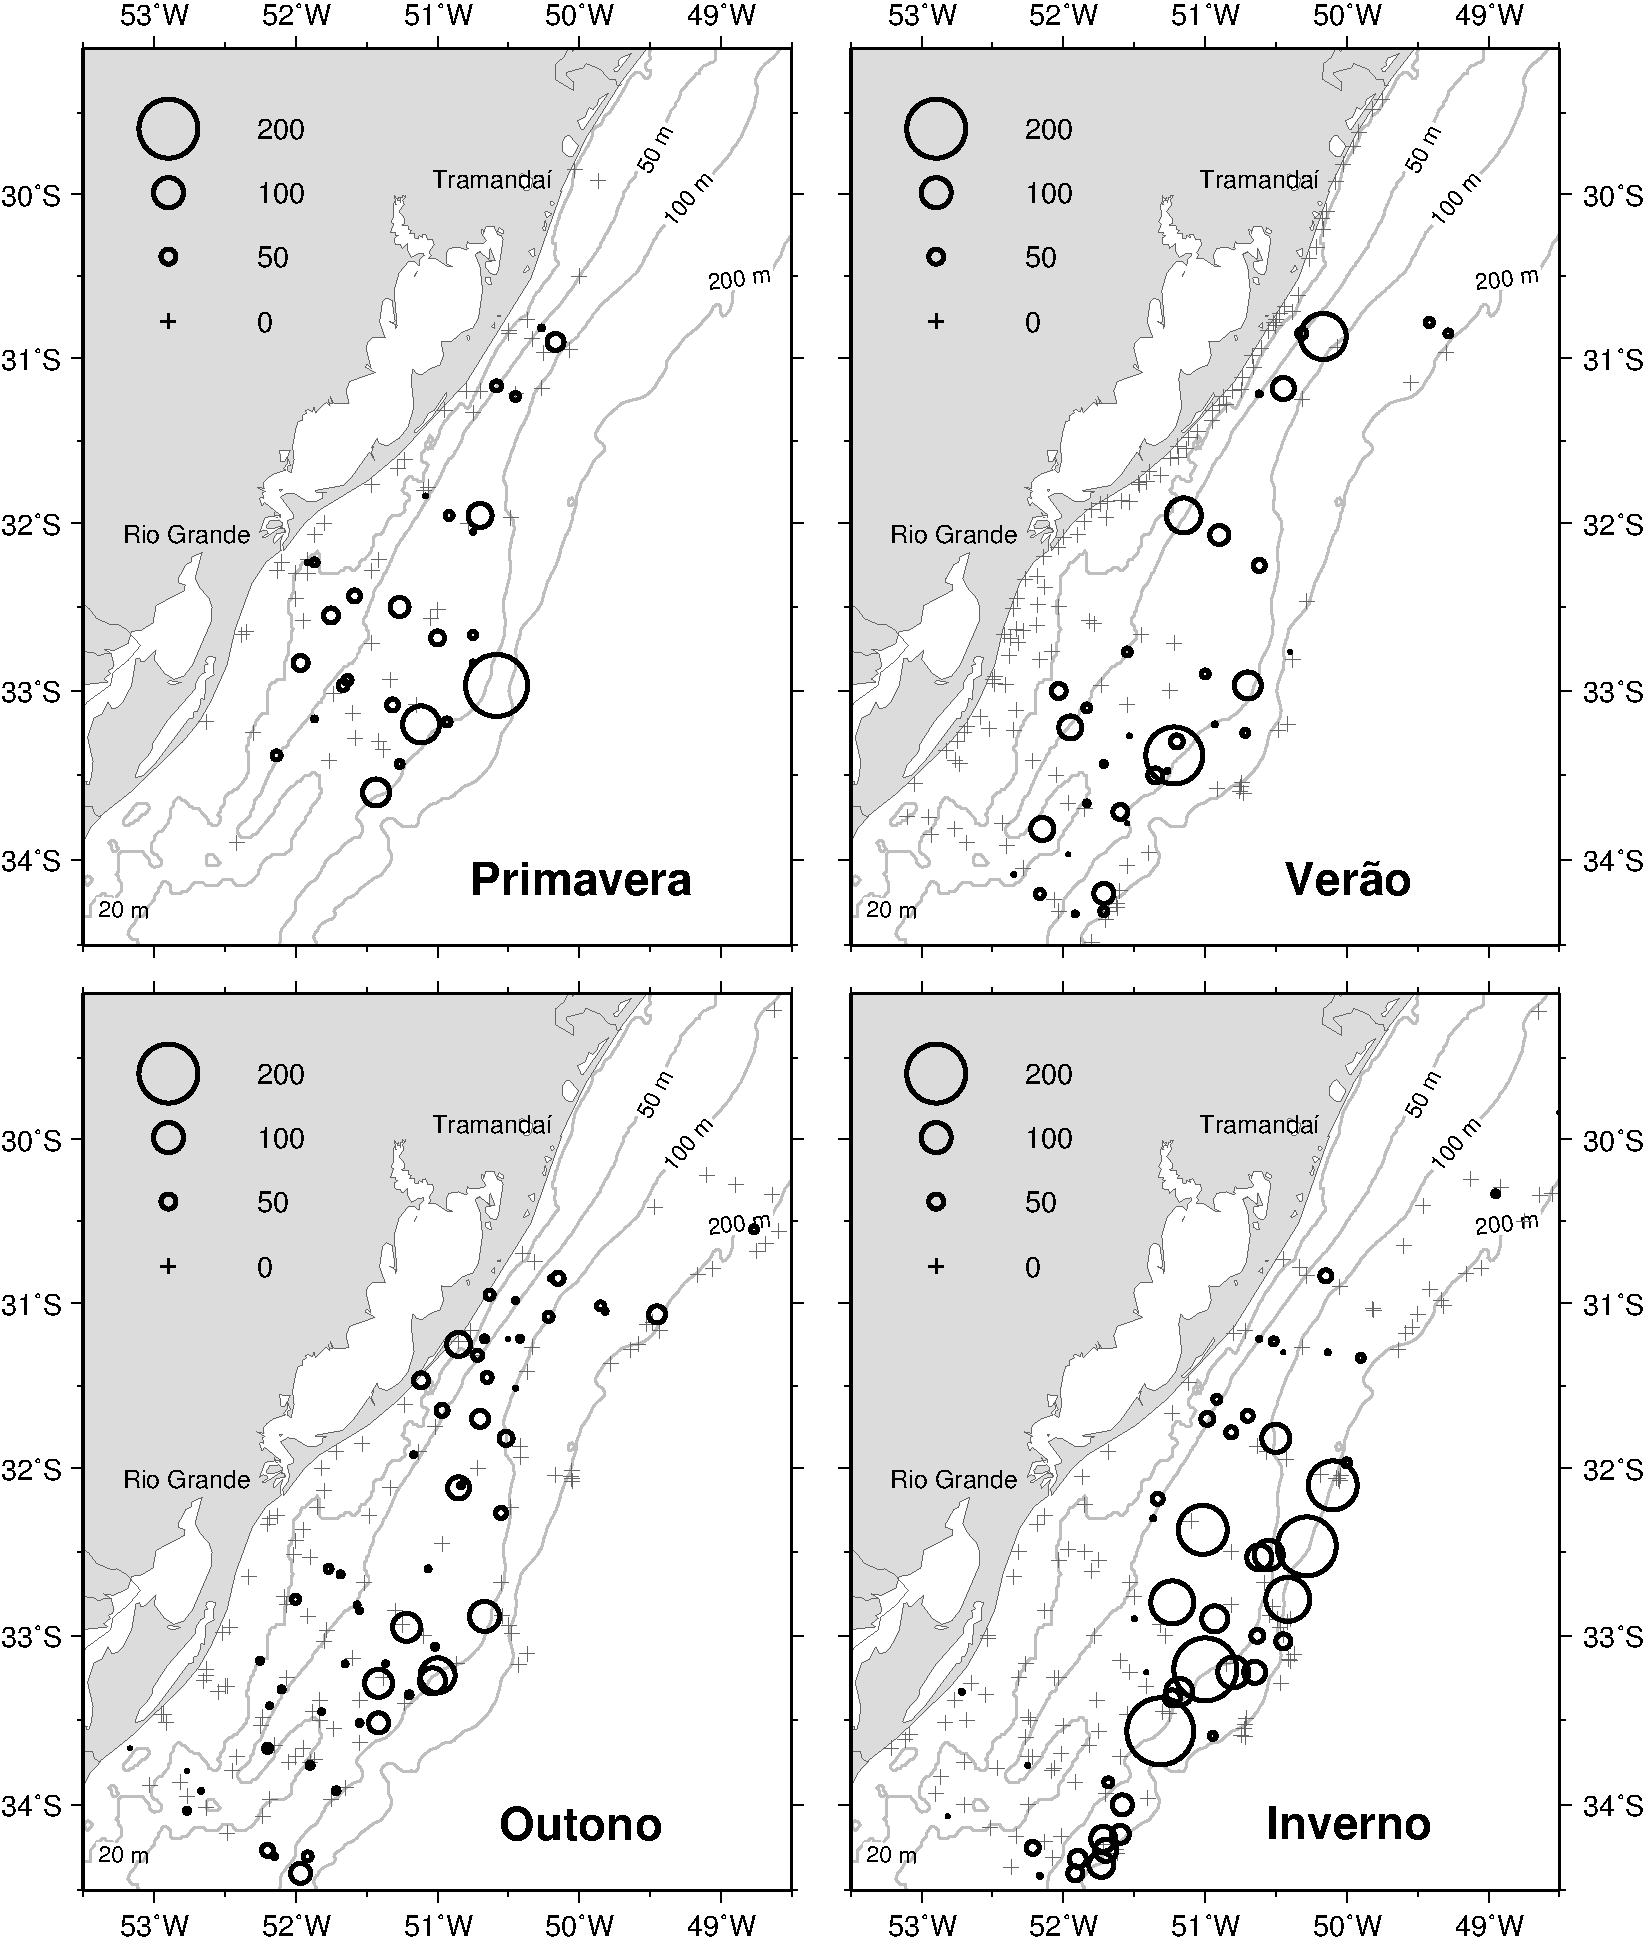
\includegraphics[width=\textwidth]{OCCULTA_MAPA_DISTRIBUICAO_CPUE}
\end{center}
\caption[Variação sazonal da distribuição espacial da CPUE em kg/hora, do cação-anjo-de-asa-curta \emph{Squatina occulta}]
	{A variação sazonal da distribuição espacial da CPUE em kg/hora, do cação-anjo-de-asa-curta \emph{Squatina occulta} 
	 na Plataforma Sul, nos levantamentos com arrasto de fundo nos anos de 1980--2005. 
	 As cruzes indicam as posições das estações de arrasto de fundo sem captura da espécie.}
\label{fig:occulta-mapacpue}
\end{figure}

%%%
	  
\emph{Squatina occulta} ocorre nas profundidades de 10 a 350~m, mas é abundante somente 
na plataforma média e externa (Figuras~\ref{fig:fo-occulta-profundidade}~e~\ref{fig:occulta-mapacpue}). % FO por prof e mapa CPUEs
Densidades de 100 a 200~kg/h ocorreram ao longo do ano nas profundidades de 50 a 200~m 
em toda a área entre as latitudes de 31°S e 34°S. Não houve evidência de migração 
sazonal entre profundidades (Figuras~\ref{fig:occulta-mapacpue}~e~\ref{fig:occulta-cpueportrimestre}). % mapa CPUEs e graf CPUE x Prof por epoca do ano
Indivíduos com CT de 100 a 130~cm constituíram a maior parte das capturas dos levantamentos 
com arrasto nos anos de 1981 a 1991 \citep{silva1996}. % (Silva, 1996). 
\emph{S. occulta} ocorreu principalmente em temperaturas de 14 a 19°C ao longo do ano, 
o que corresponde à maior profundidade do seu hábitat em comparação com \emph{S. guggenheim} (Figura~\ref{fig:occulta-distrib-tempfundo}). % FO por Temp
Nos levantamentos da plataforma foram capturados ao todo nove neonatos com CT de 29 a 42~cm, 
nos meses de janeiro a agosto e sempre nas profundidades de 60 a 80~m, com os menores neonatos 
nos meses de janeiro e fevereiro \citep{silva1996}. % (Silva, 1996). 
A baixa abundância de neonatos é atribuída ao longo ciclo reprodutivo da fêmea, que 
realiza o parto apenas uma vez a cada 4 ou 5 anos da sua vida adulta. 
\emph{S. occulta} é uma espécie sedentária da plataforma média e externa, onde seu berçário 
está situado nas profundidades de 60 a 80~m. A pesca na plataforma média e externa atinge 
ao longo do ano toda a população de \emph{S. occulta} da Plataforma Sul (Capítulo~\ref{chap:pesca-industrial}). % , Figura~\ref{fig:ct-occulta}).  % Distr. de CT na pesca industrial

%
% VARIAÇÃO SAZONAL DA CPUE (Kg/h)
%
%%%%%%%%%%%%%%%%%%%%%%%%%%%%%%%%%%%%%%%%%%%%%%%%%%%%%%%%%%%%%%%

\begin{figure}
\begin{center}
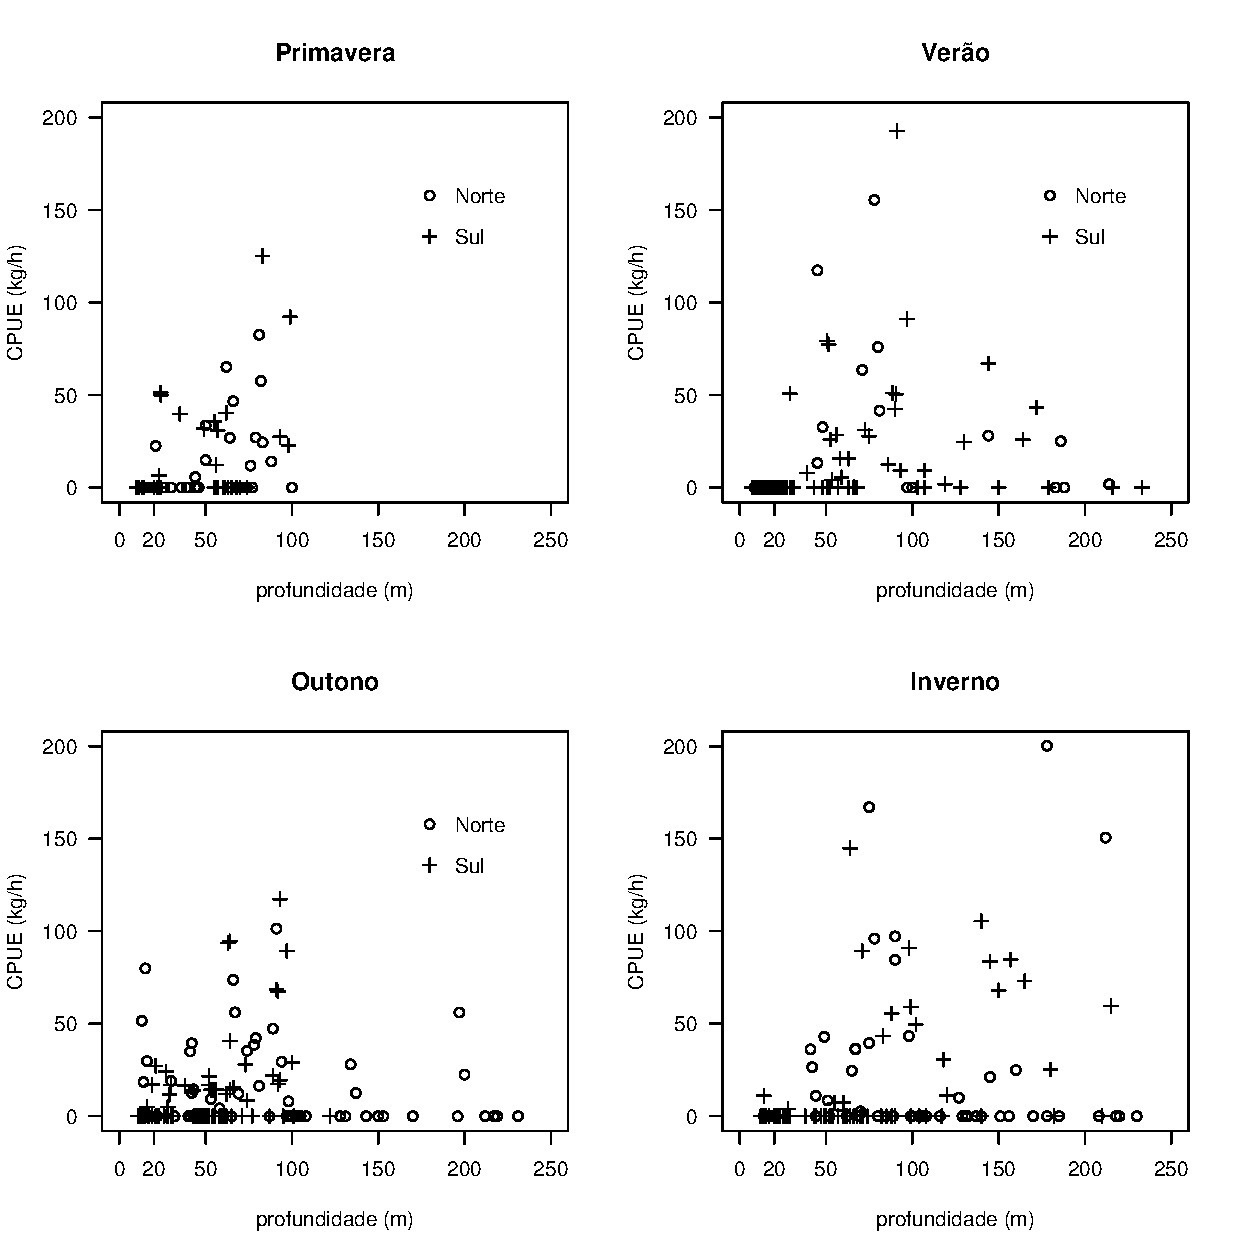
\includegraphics[width=\textwidth]{OCCULTA_CPUEXPROFTRIMESTRES}
\end{center}
\caption[Variação sazonal da densidade populacional do cação-anjo-de-asa-curta \emph{Squatina occulta}]
	{A variação sazonal da densidade populacional do cação-anjo-de-asa-curta \emph{Squatina occulta} 
	 nas diferentes profundidades da Plataforma Sul, ao norte e ao sul da perpendicular de Rio Grande. 
	 Cada ponto é a Captura por Unidade de Esforço (CPUE) em kg/hora, de uma 
	 estação de pesca de arrasto de fundo nos anos de  1980--2005.}
\label{fig:occulta-cpueportrimestre}
\end{figure}

%%%

%
% FO DE S OCCULTA POR TEMPERATURA DE FUNDO
%
%%%%%%%%%%%%%%%%%%%%%%%%%%%%%%%%%%%%%%%%%%%%%%%%%%%%%%%%%%%%%%%

\begin{figure}
\begin{center}
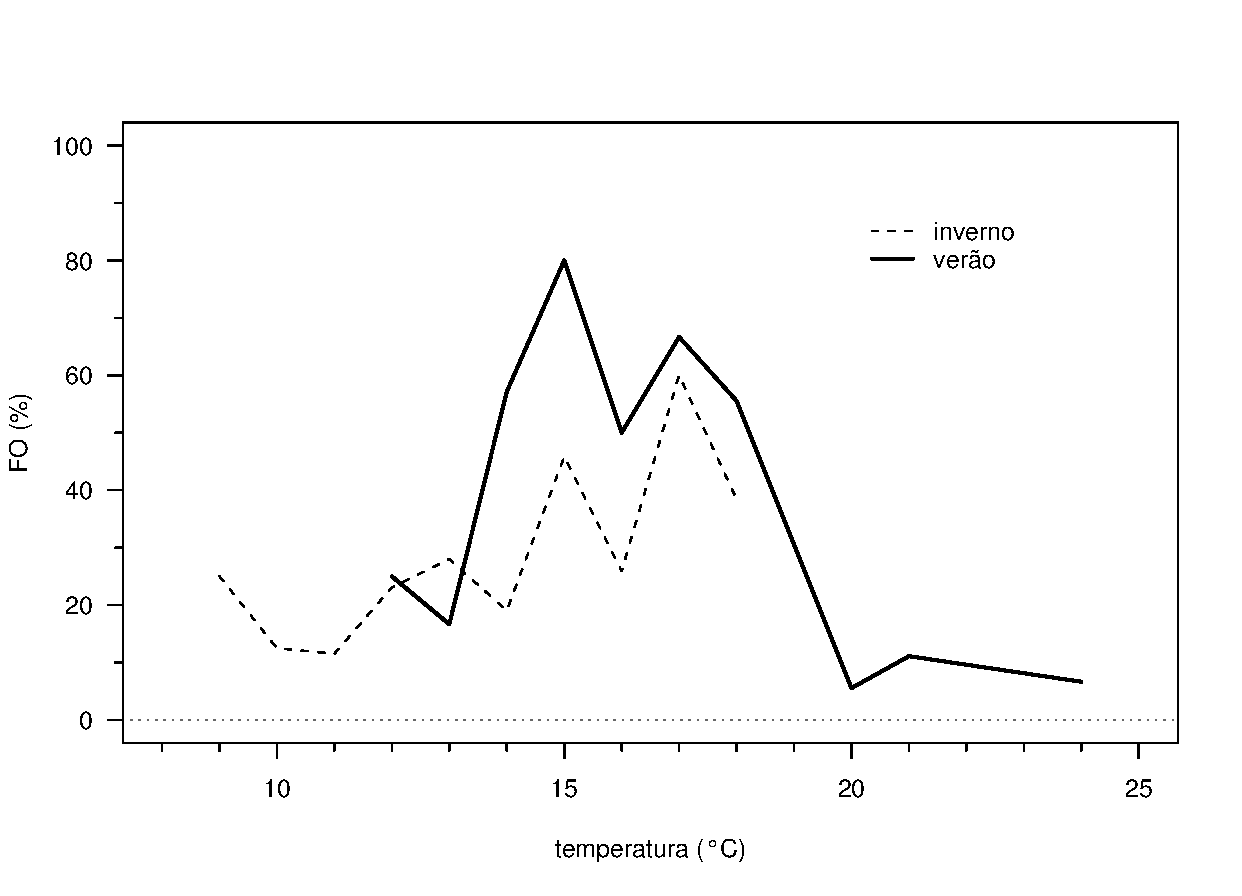
\includegraphics[width=\textwidth]{OCCULTA_DISTRIBTEMPFUNDO}
\end{center}
\caption[Freqüência de ocorrência (FO) do cação-anjo-de-asa-curta \emph{Squatina occulta}
	 com relação à temperatura de fundo]
	{Freqüência de ocorrência (FO) do cação-anjo-de-asa-curta \emph{Squatina occulta}
	 com relação à temperatura de fundo, nos levantamentos com 
	 arrasto de fundo nos anos 1980--2005.}
\label{fig:occulta-distrib-tempfundo}
\end{figure}

%%%

\section*{Distribuição e pesca de  \emph{Squatina argentina}}

Uma população regional de \emph{S. argentina} ocorre ao longo do ano na plataforma externa e no talude 
superior de toda a Plataforma Sul, nas profundidades de 100 a 400~m, mas com sua maior abundância 
nas profundidades de 180 a 250~m entre Rio Grande e Chuí. Indivíduos de ambos os sexos e em todos 
os estágios de vida ocorrem na área (Tabela~\ref{tab:anjos-parpopulacionais}), % (Tabela 5.2), 
e a captura de dois neonatos, com CT de 35 e 37~cm 
respectivamente, em 300~m de profundidade na latitude de 29°S em maio de 1987, é evidência de que 
a espécie reproduz no talude da Plataforma Sul \citep[dados pretéritos FURG]{silva1996,vooren1997}. % (Silva, 1996; Vooren, 1997; dados pretéritos FURG). 
A espécie não foi encontrada nos desembarques da pesca industrial com arrasto de fundo de Rio Grande 
em 1994--1995. Esses desembarques foram oriundos das profundidades de 10 a 150~m, fora do hábitat principal 
de \emph{S. argentina} \citep{vieira1996}. % (Vieira, 1996). 
\citet{perez2005} informam que em 2001, \emph{S. argentina} foi captura 
incidental na pescaria direcionada ao peixe-sapo \emph{Lophius gastrophysis} com redes de emalhe de fundo nas 
profundidades de 130--600~m, entre Rio de Janeiro e Chuí. Isto confirma a distribuição batimétrica 
de \emph{S. argentina} e a vulnerabilidade de cações-anjo à pesca com redes de emalhe. A pescaria direcionada 
de cações-anjo, com redes de emalhe de fundo na plataforma externa e no talude superior, desenvolveu-se 
rapidamente na Plataforma Sul na década de 1990 (Capítulo~\ref{chap:pesca-industrial}). 
Essa pescaria operava no hábitat de \emph{S. argentina}. 


% \section*{\emph{Squatina argentina}: a distribuição espacial e temporal}
% 
% \emph{S. argentina} ocorre nas profundidades de 100 a 400~m da Plataforma Sul 
% e do talude continental adjacente \citep{vooren1997}. % (Vooren 1997). 
% Nos levantamentos da plataforma externa e do talude com arrasto de fundo no inverno de 1986 
% e no outono de 1987, a espécie ocorreu nessas profundidades entre as latitudes de 32°00'S e 34°20'S. 
% A densidade de \emph{S. argentina} nessa área variou muito, entre as médias de 22,8~kg/h no inverno 
% de 1986 e de 62,1~kg/h no outono de  1987, enquanto as quatro ocorrências da espécie no outono 
% de 1987 foram uma captura de 1.078~kg e mais três capturas de 19 a 50~kg. 
% A espécie ocorreu em  42\% das estações de arrasto no inverno de 1986, e em 21\% das estações 
% no outono de 1987 \citep{vooren2002}. % (Vooren e Lamónaca 2002). 
% Essas grandes variações da densidade e da freqüência 
% de ocorrência de \emph{S. argentina} foram fenômenos naturais, porque nos anos de 1986 e 1987 a intensidade 
% da pesca comercial na plataforma externa e no talude era baixa. Juvenis e adultos de ambos os 
% sexos ocorreram nas capturas. Apenas um neonato foi capturado, com CT de 37,5~cm e na 
% profundidade de 260~m, e apenas 10\% das fêmeas adultas estavam prenhes \citep{silva1996}. % (Silva, 1996). 
% \emph{S. argentina} ocorre ao longo do ano na plataforma externa e no talude superior, principalmente 
% entre Rio Grande e Chuí, mas com grande variação espacial e temporal da sua abundância, 
% e com baixa incidência de reprodução. A maneira irregular como \emph{S. argentina} ocorreu no sul 
% do Brasil nos anos de 1986 e 1987 pode refletir a dispersão da espécie para uma área situada 
% na margem da sua distribuição geográfica. As variações temporais da abundância de \emph{S. argentina} 
% no sul do Brasil não têm interpretação com relação ao status de conservação 
% da espécie nessa região. 

% \section*{O status de conservação de \emph{Squatina guggenheim} e  \emph{Squatina occulta}}

\section*{O status de conservação de \emph{Squatina guggenheim}, \emph{S. occulta} e \mbox{\emph{S. argentina}}}

As populações de \emph{S. guggenheim}, \emph{S. occulta} e \emph{S. argentina} da Plataforma Sul 
fazem parte da distribuição contínua dessas espécies desde o Rio de Janeiro até a Argentina. 
Porém na Plataforma Sul essas espécies são 
sedentárias e realizam todo seu ciclo de vida dentro da área. 
Por isto, e pelo modo de vida territorial do indivíduo e o lento crescimento populacional 
dos cações-anjo em geral, infere-se que as populações dessas espécies das áreas vizinhas 
também são sedentárias e mantêm seu equilíbrio entre nascimentos e mortes mediante o recrutamento 
dentro de cada área, sem a produção de um importante excesso de recrutas que poderiam emigrar para 
outras áreas. Portanto, um eventual movimento de dispersão ou migração entre populações vizinhas 
é de baixa intensidade, e não tem um impacto em curto prazo sobre a abundância dessas populações. 
As populações de \emph{S. guggenheim}, \emph{S. occulta} e \emph{S. argentina} da Plataforma Sul 
são unidades em termos do manejo da pesca e da conservação da biodiversidade. 
A conservação das populações de \emph{S. guggenheim}, \emph{S. occulta} e \emph{S. argentina} 
da Plataforma Sul é de elevada importância para a conservação dessas espécies na região sudoeste 
do Oceano Atlântico.  

Nas estatísticas da pesca dos portos de Rio Grande e Itajaí, as diversas espécies de cação-anjo são 
agrupadas na única categoria ``cação-anjo''.  No porto de Rio Grande os desembarques de cação-anjo 
pela pesca industrial com arrasto de fundo são constituídos de \emph{S. guggenheim} 
e \emph{S. occulta} \citep{vieira1996,miranda1999}. % (Vieira, 1996; Miranda, 1999). 

A CPUE de cações-anjo das frotas de arrasto simples e de arrasto de parelha de Rio Grande 
não varia sazonalmente \citep{miranda2003}. % (Miranda e Vooren, 2003). 
Isto está em concordância com o fato de que \emph{S. occulta} é uma espécie sedentária 
da plataforma média e externa, enquanto somente uma parte da população de \emph{S. guggenheim} 
migra sazonalmente entre a plataforma interna e as águas costeiras. Cações-anjo ocorrem 
durante o ano todo nas áreas de pesca das frotas de arrasto.

Ao longo dos anos a pescaria da frota de arrasto simples de Rio Grande foi direcionada 
a um conjunto de espécies abundantes de peixes ósseos (Tabela~\ref{tab:anjo-percentual-arrasto-simples}). % (Tabela 5.3).  
Após 1980 a proporção de cações-anjo nas capturas do arrasto simples aumentou até cerca 
de 6\% e permaneceu nesse nível até 1990. Durante uma viagem de pesca do arrasteiro 
simples ``Santa Luiza'' em agosto de 1989, uma corrente de aço foi montada no cabo inferior 
da boca da rede, com a finalidade de assim aumentar a eficiência da rede para a captura 
de cações-anjo, embora peixes ósseos continuaram sendo o alvo da pescaria\footnote{Vooren, C. M. (não publicado)}. 
O aumento das capturas de cações-anjo pelo arrasto simples após 1980 com certeza reflete 
um maior interesse na captura desses peixes, mas a pescaria permaneceu direcionada aos peixes ósseos, 
e capturava cações-anjo porque estes também ocorreram na área de pesca. 
O aumento da CPUE de cações-anjo pelo arrasto simples nos anos de 1975 a 1988 reflete um 
aumento da captura incidental de cações-anjo na pescaria mista direcionada a um conjunto 
de abundantes peixes ósseos (Figura~\ref{fig:anjos-cpuesafra-1975a2002}).  % Variação anual da CPUE em RG de arrasto simples e parelha
O declínio da CPUE do arrasto simples após 1988 reflete uma redução dessa captura incidental 
e portanto, uma redução da abundância de cações-anjo na área de pesca do arrasto simples 
na Plataforma Sul. Somente em 1987 houve talvez pesca direcionada a cações-anjo 
pelo arrasto simples (Tabela~\ref{tab:anjo-percentual-arrasto-simples}).
Por esse motivo, a CPUE do arrasto simples em 1987 não é considerada 
na presente análise.

% TABELA 5.3

%
%  TABELA PERCENTUAL DE ANJOS NO ARRASTO SIMPLES
%
%%%%%%%%%%%%%%%%%%%%%%%%%%%%%%%%%%%%%%%%%%%%%%%%%%%%%%%%

\begin{table}
\caption[Composição dos desembarques da frota de arrasto simples no porto de Rio Grande]
        {Composição dos desembarques da frota de arrasto simples no porto de Rio Grande. 
         Fontes: \citet{haimovici1997,miranda2003,ceperg2003}.} % Haimovici (1997), Miranda e Vooren (2003), CEPERG (2002).}  
\label{tab:anjo-percentual-arrasto-simples}
\begin{tabularx}{\textwidth}{XXX}
\toprule
			& \% cação-anjo				& \% castanha, pescada-olhuda 
								   e pescadinha 		\\
\midrule
1975--1979		& 3,5 (2,6-4,1)				& 63,3 (41,0-71,1)		\\
\addlinespace
1980--1986		& 6,2 (5,3-7,2)				& 65,8 (55,7-73,3)		\\
\addlinespace
1987			& 9,5					& 46,5				\\
\addlinespace
1990			& 5,4					& 48,1				\\
\addlinespace
2001			& 0,5					& 79,0				\\
\bottomrule
\end{tabularx}
\end{table}

%%%%%%%%

% FIGURA 5.16
% área de pesca. O aumento da CPUE de cações-anjo pelo arrasto simples nos anos de 1975 a 1988 reflete 
% um aumento da captura incidental de cações-anjo na pescaria mista direcionada a um conjunto de 
% abundantes peixes ósseos (Figura~\ref{fig:anjos-cpuesafra-1975a2002}).  % Variação anual da CPUE em RG de arrasto simples e parelha
%
%
%%%%%%%%%%%%%%%%%%%%%%%%%%%%%%%%%%%%%%%%%%%%%%%%%%%%%%

\begin{figure}
\begin{center}
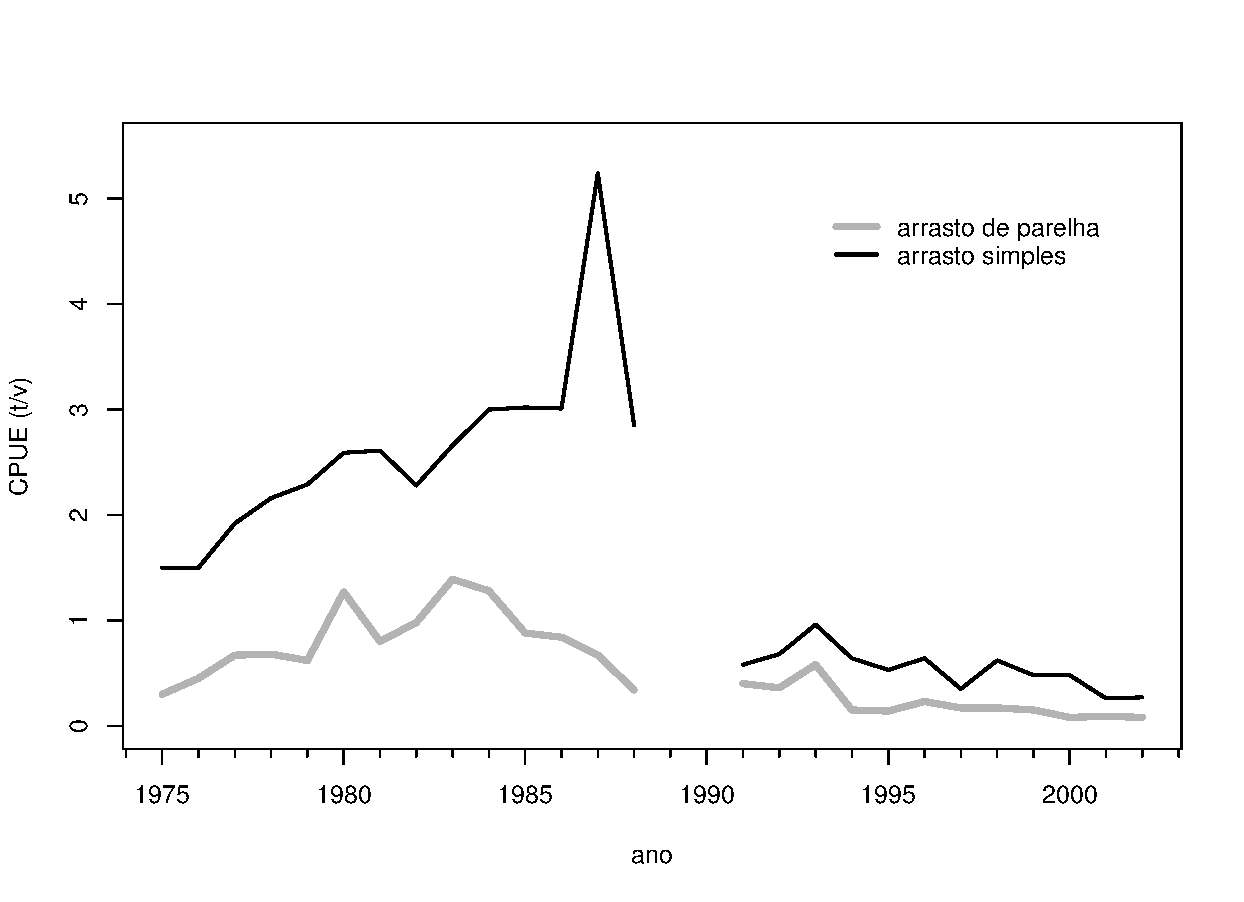
\includegraphics[width=\textwidth]{CPUESAFRAANJOS}
\end{center}
\caption[Captura por Unidade de Esforço (CPUE) em ton/viagem, 
	 dos cações-anjo \emph{Squatina guggenheim} e \emph{Squatina occulta}, em conjunto, na Plataforma Sul, 
	 pelas frotas de arrasto simples e arrasto de parelha de Rio Grande]
	{Captura por Unidade de Esforço (CPUE) em ton/viagem, 
	 dos cações-anjo \emph{Squatina guggenheim} e \emph{Squatina occulta}, em conjunto, na Plataforma Sul, 
	 pelas frotas de arrasto simples (abril-setembro) e arrasto de parelha (dezembro-março)
	 que desembarcaram no porto de Rio Grande. Fontes: \citet{miranda2003,ceperg2003}.}
\label{fig:anjos-cpuesafra-1975a2002}
\end{figure}

%%%
 
Na pescaria pela frota de arrasto de parelha de Rio Grande, os cações-anjo sempre 
constituíram uma pequena captura incidental, com porcentagens de 0,9 a 3,1\% na 
captura total nos anos de 1975 a 1988,  e de menos de 1\% 
desde 1991 \citep{haimovici1997,miranda2003}. % (Haimovici, 1997; Miranda e Vooren, 2003).  
A CPUE de cações-anjo pela frota de arrasto de parelha de Rio Grande reflete a abundância 
desses peixes na área de pesca dessa frota ao longo dos anos de 1975 a 2002. 

A variação temporal da CPUE do arrasto foi analisada pela comparação dos períodos 
de alta CPUE (anos 1980--1988) e de baixa CPUE (anos 1997--2002). 
Os dois conjuntos independentes de dados resultam no declínio da CPUE de cerca de 85\% (Tabela~\ref{tab:anjos-cpue-variacao}). 
Pela linha de tendência da CPUE científica na Plataforma Sul como um todo, a estimativa 
do declínio da abundância de \emph{S. guggenheim} foi de 87\% entre os anos de 1980 e 2000, 
enquanto para \emph{S. occulta} o declínio foi de cerca de 50\% (Figura~\ref{fig:anjos-cpue-porano-dadospreteritos}). % (Fig. 5.15). 
Porém a análise detalhada de dois conjuntos independentes de dados da pesca científica 
nas profundidades de 100--500~m constitui evidência de que entre 1986 e 2002 
a abundância de \emph{S. occulta} e de \emph{S. argentina} sofreu um declínio de cerca 
de 80\% na plataforma externa e no talude superior ou seja, no hábitat principal 
dessas espécies (Tabela~\ref{tab:anjos-cpue-cientifica-variacao}).  % TABELA NOVA VOOREN 
Os dados da pesca científica e da pesca comercial em conjunto são evidência de que 
entre 1986 e 2002 ocorreu um declínio de cerca de 85\% da população de \emph{S. guggenheim}, 
e de 80\% das populações de \emph{S. occulta} e \emph{S. argentina} da Plataforma Sul. 
\emph{S. guggenheim} foi classificado pela IUCN como ``em perigo'' no Brasil, 
\emph{S. occulta} como ``em perigo'' e \emph{S. argentina} 
como ``deficiente de dados'' \citep{chiaramonte2004a,chiaramonte2004b,chiaramonte2004c}, % (Chiaramonte, 2000a, 2000b, 2000c), 
porém no ano de 2000 os dados sobre o declínio dessas espécies no Brasil não estavam disponíveis. 
Com esses novos dados, as três espécies estão criticamente ameaçadas no Brasil. 
A conservação de \emph{S. guggenheim}, \emph{S. occulta} e \emph{S. argentina} da Plataforma Sul 
é urgente para a conservação dessas espécies na região sudoeste do Oceano Atlântico.

% TABELA 5.4 DECLINIO DA CPUE EM 85%
%
% TABELA VARIAÇÃO DA CPUE DOS CACOES ANJO NO ARRASTO SIMPLES E DE PARELHA
%
%%%%%%%%%%%%%%%%%%%%%%%%%%%%%%%%%%%%%%%%%%%%%%%%%%%%%%%%%%%%%%%%%%%%%%%%%%%%

\begin{table}
\caption[Média e amplitude dos valores anuais da captura por unidade de esforço, 
         em ton/viagem, dos cações-anjo \emph{Squatina guggenheim} e \emph{S. occulta}, em conjunto, 
	 pelas frotas de arrasto simples 
	 e arrasto de parelha que desembarcaram no porto de Rio Grande]
        {Média e amplitude dos valores anuais da captura por unidade de esforço, 
         em ton/viagem, dos cações-anjo \emph{Squatina guggenheim} e \emph{S. occulta}, em conjunto, 
	 pelas frotas de arrasto simples 
	 e arrasto de parelha que desembarcaram no porto de Rio Grande. 
	 Fontes: \citet{miranda2003,ceperg2003}.} % Miranda e Vooren 2003 e IBAMA/CEPERG.}
\label{tab:anjos-cpue-variacao}
\begin{center}
\begin{tabular*}{\textwidth}{l@{\extracolsep{\fill}}ll}
\toprule
Anos 				& Arrasto simples		& Arrasto de parelha	\\
				& safra: ano todo		& safra: ano todo	\\
\midrule
 1980-1988 (8 anos) 		& 2,75 (2,59-3,02)		& 0,94 (0,34-1,39)	\\
\addlinespace
 1997-2002 (6 anos)  		& 0,41 (0,26-0,62) 		& 0,12 (0,08-0,17)	\\
\midrule
 1997-2002 como \% de 80-88 	& 15\%				& 13\%			\\
\bottomrule
\end{tabular*}
\end{center}
\end{table}

%%%

% FIGURA 5.15 VARIACAO ANUAL DA CPUE CIENTÍFICA
%
% CPUE ANUAL DOS CACOES ANJO ENTRE 1980 E 2005 DADOS PRETERITOS
%
%%%%%%%%%%%%%%%%%%%%%%%%%%%%%%%%%%%%%%%%%%%%%%%%%%%%%%%%%%%%%%%%%

\begin{figure}
\begin{center}
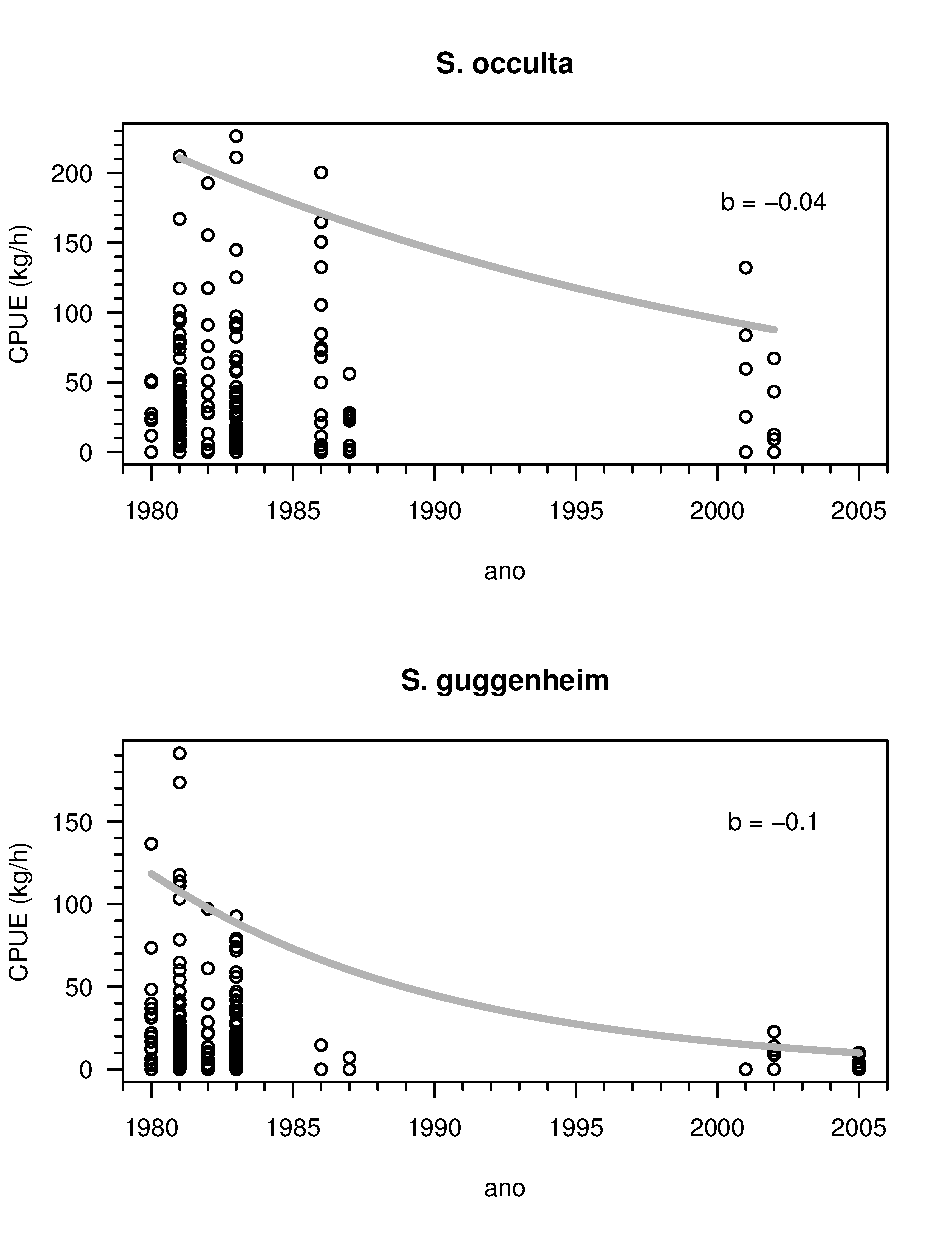
\includegraphics[width=0.8\textwidth]{ANJOS_CPUEXDECADAS}
\end{center}
\caption[Variação temporal da Captura por Unidade de Esforço em kg/hora de arrasto de fundo, 
	 do cação-anjo-espinhoso \emph{Squatina guggenheim} e do cação-anjo-de-asa-curta \emph{S. occulta} 
	 na Plataforma Sul]
	{A variação temporal da  Captura por Unidade de Esforço (CPUE) em kg/hora, 
	 do cação-anjo-espinhoso \emph{Squatina guggenheim} e do cação-anjo-de-asa-curta \emph{S. occulta} 
	 na Plataforma Sul. 
	 Cada ponto é a CPUE de uma estação de arrasto de fundo em levantamentos 
	 nos anos 1980--2005. As linhas de tendência são ajustadas aos valores 
	 da CPUE máxima de cada ano ($CPUE_{t} = CPUE_{0} \times e^{bt}$).}
\label{fig:anjos-cpue-porano-dadospreteritos}
\end{figure}

%%%


% TABELA 5.5 TABELA NOVA VOOREN VER DOC
%
%%%%%%%%%%%%%%%%%%%%%%%%%%%%%%%%%%%%%%%%%%%%%%%%%%%%%%%%%%%%%%%%%%%%%%%%%%%%

\begin{table}
\caption[Captura por unidade de esforço (CPUE), freqüência de ocorrência (FO em \%) 
         e o declínio desses parâmetros entre 1986 e 2002, de \emph{Squatina occulta}
         e \emph{S. argentina}]
        {Captura por unidade de esforço (CPUE), freqüência de ocorrência (FO em \%) 
         e o declínio desses parâmetros entre 1986 e 2002, de \emph{Squatina occulta}
         e \emph{S. argentina} nas profundidades de 100--500~m entre Cabo de Santa Marta Grande e Chuí, 
         nos levantamentos com arrasto de fundo do Projeto TALUDE em 1986--1987 com arraçal 
         de 28~m (dados pretéritos FURG) e do Programa REVIZEE em 2001--2002 
         com arraçal de 38~m \citep{haimovici2002}.
         N = número de estações de pesca. 
         Os dados do Projeto TALUDE foram padronizados para um arraçal de 38~m.}
\label{tab:anjos-cpue-cientifica-variacao}
\begin{center}
\begin{footnotesize}
\begin{tabular*}{\textwidth}{l@{\extracolsep{\fill}}ccccccc}
\toprule
		& N 		& \multicolumn{3}{c}{\emph{Squatina occulta}}	& \multicolumn{3}{c}{\emph{Squatina argentina}}	\\
\cmidrule(r){3-5}  \cmidrule(l){6-8}
		& 		& CPUE kg/h	& CPUE Nº/h	& FO\%	& CPUE kg/h	& CPUE Nº/h	& FO\%	\\
\midrule
Inverno 1986	& 36		& 25,0		& 2,6		& 56,6	& 21,7		& 1,5		& 45,2	\\
Inverno 2001	& 51		& 4,8		& 0,3		& 7,8	& 5,5		& 0,5		& 1,4	\\
\addlinespace
Declínio (\%)	& 		& 81		& 89		& 86	& 75		& 67		& 97	\\
\midrule
Outono 1987	& 30		& 10,2		& 1,1		& 45,2	& 41,5		& 3,9		& 22,7	\\
Outono 2002	& 48		& 2,2		& 0,3		& 8,3	& 1,5		& 0,3		& 8,3	\\
\addlinespace
Declínio (\%)	& 		& 78		& 73		& 82	& 96		& 92		& 63	\\
\bottomrule
\end{tabular*}
\end{footnotesize}
\end{center}
\end{table}

%%%%%%%%%%%%%%%%%%%%%%%%%%

A captura anual de cação-anjo pela frota pesqueira do porto de Rio Grande aumentou desde 736~t 
no ano de 1975 até 2.139~t em 1987 (Figura~\ref{fig:anjos-desembarques-1975a2002}). % (Fig. 5.18). 
O declínio das populações de \emph{S. guggenheim} e \emph{S. occulta} ocorreu simultaneamente 
com um grande aumento da pescaria de ambas essas espécies. No ano de 1995, as taxas de mortalidade 
excederam as taxas de crescimento populacional de tal maneira que as taxas anuais de declínio 
da população foram de 16\% e 11\% em respectivamente \emph{S. guggenheim} e \emph{S. occulta} \citep{vieira1996}. % (Vieira, 1996). 
A pesca foi o fator responsável pelo declínio dessas espécies na Plataforma Sul. 
Para a conservação de \emph{S. guggenheim} e \emph{S. occulta}, essas espécies precisam da maior 
proteção possível da pesca na Plataforma Sul.

% FIGURA 5.18 DESEMBARQUES ANUAIS DESDE 1975
%
% DESEMBARQUES TOTAIS DE CAÇÕES ANJO
%
%%%%%%%%%%%%%%%%%%%%%%%%%%%%%%%%%%%%%%%%%%%%%%%%%%%%%%

\begin{figure}
\begin{center}
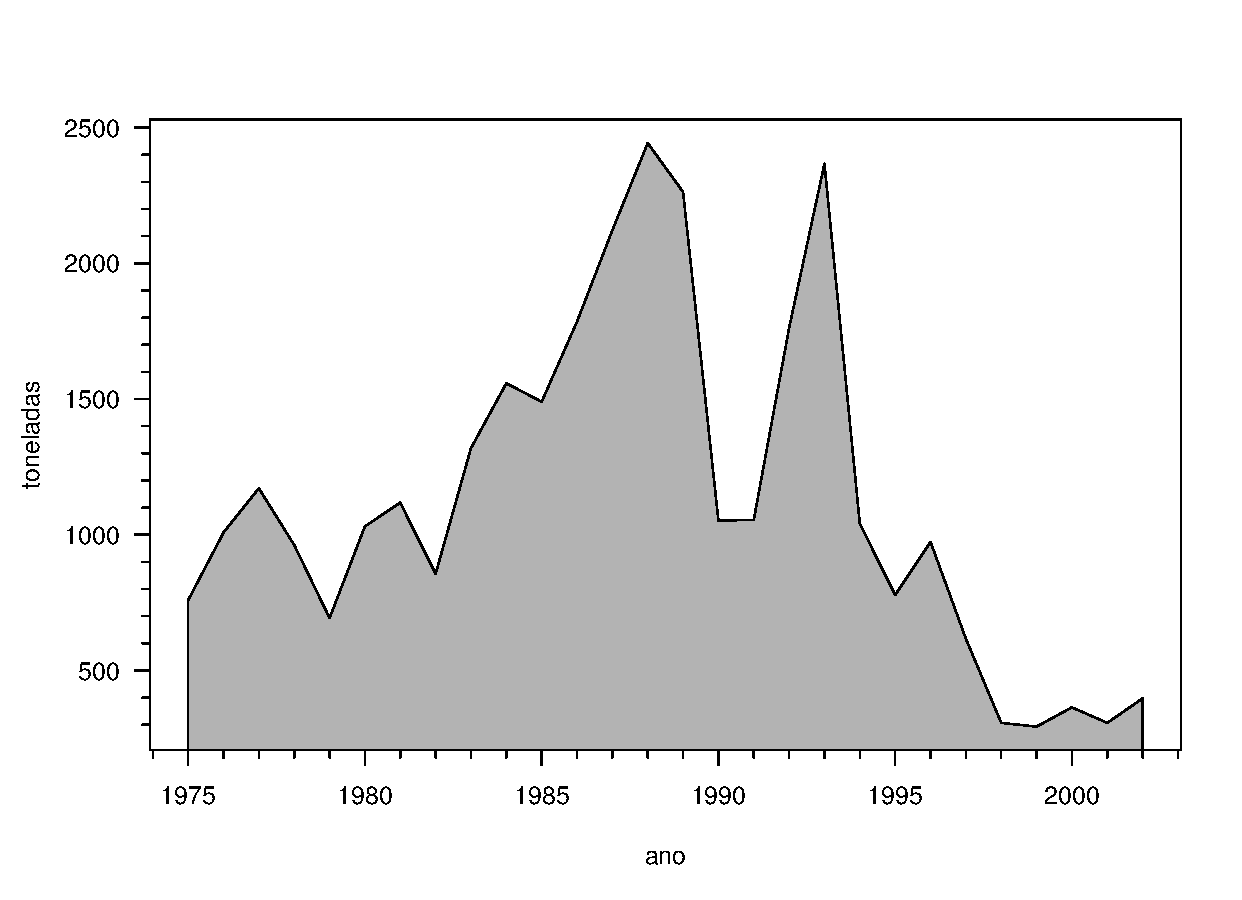
\includegraphics[width=\textwidth]{DESEMBARQUESTOTAISANJOS}
\end{center}
\caption[A variação temporal da captura anual dos cações-anjo \emph{Squatina guggenheim} 
	e \emph{Squatina occulta}, em conjunto, 
        desembarcada no porto de Rio Grande
	pela pesca artesanal e industrial 
	nos anos de 1975 a 2002.]
	{A variação temporal da captura anual dos cações-anjo \emph{Squatina guggenheim} 
	e \emph{Squatina occulta}, em conjunto, 
        desembarcada no porto de Rio Grande
	pela pesca artesanal e industrial 
	nos anos de 1975 a 2002. Fonte: IBAMA/CEPERG.}
\label{fig:anjos-desembarques-1975a2002}
\end{figure}

%%%

O segundo pico de captura total, de 2.296~t no ano de 1993, foi devido a uma nova pescaria 
com redes de emalhe que surgiu em torno de 1990 e que foi direcionada a cações. 
Essa pescaria obteve grandes capturas de cação-anjo nos anos 1992--1997, com desembarques 
anuais  de até 1.079~t e com CPUE anual de até 5,2~t/viagem \citep[Figura~\ref{fig:anjos-desembarques-1975a2002}]{miranda2003}. % (Fig. 5.18; Miranda e Vooren, 2003). 
Essa pescaria operava na plataforma externa e no talude superior (Capítulo~\ref{chap:pesca-industrial}).
O fato de que os rendimentos dessa pescaria decaíram após seis anos de pesca é evidência do 
seu forte impacto sobre as populações de \emph{S. argentina}  e \emph{S. occulta}.
O declínio dessas espécies na plataforma externa e no talude (Tabela~\ref{tab:anjos-cpue-cientifica-variacao}) % NOVA TABELA VOOREN
é atribuído a essa pescaria.

% A Plataforma Sul faz parte da área contínua de distribuição de \emph{S. guggenheim} e \emph{S. occulta} 
% desde o Rio de Janeiro até o Uruguai e, no caso de \emph{S. guggenheim}, até a Argentina. Porém na 
% Plataforma Sul cada uma dessas duas espécies realiza todo o seu ciclo de vida, 
% e ocorre ao longo do ano com a mesma abundância. Por isto, e pelo modo 
% de vida sedentário e o lento crescimento populacional dos cações-anjo em geral, infere-se 
% que as populações de \emph{S. guggenheim} e \emph{S. occulta} das áreas vizinhas também são unidades regionais 
% e mantêm seu equilíbrio entre nascimentos e mortes mediante o recrutamento dentro de cada área, 
% sem a produção de um importante excesso de indivíduos que podem emigrar para outras áreas. 
% Portanto, um eventual movimento de dispersão ou migração entre populações vizinhas é de baixa 
% intensidade, e não tem um impacto em curto prazo sobre a abundância dessas populações. 
% As populações de \emph{S. guggenheim} e \emph{S. occulta} da Plataforma Sul são unidades em termos do manejo 
% da pesca e da conservação da biodiversidade, e propiciam % propiciaram
% a segunda maior pescaria de cações-anjo 
% do Atlântico Sudoeste. A conservação das populações de \emph{S. guggenheim} e \emph{S. occulta} da 
% Plataforma Sul é de elevada importância para a conservação dessas espécies na região 
% sudoeste do Oceano Atlântico. 

% Nas estatísticas da pesca dos portos de Rio Grande e Itajaí, as diversas espécies de cação-anjo 
% são agrupadas na única categoria ``cação-anjo''.  No porto de Rio Grande os desembarques de 
% cação-anjo são constituídos de \emph{S. guggenheim} e \emph{S. occulta}.  A CPUE de cação-anjo das frotas de 
% arrasto simples e de arrasto de parelha de Rio Grande não varia sazonalmente \citep{miranda2003}. % (Miranda e Vooren, 2003). 
% Isto está em concordância com o fato de que \emph{S. occulta} é uma espécie sedentária da plataforma média 
% e externa, enquanto somente uma parte da população de \emph{S. guggenheim} migra sazonalmente entre a plataforma 
% interna e as águas costeiras. Cações-anjo ocorrem durante o ano todo nas áreas de pesca 
% das frotas de arrasto. 

% Ao longo dos anos a pescaria da frota de arrasto simples de Rio Grande foi direcionada 
% a um conjunto de espécies abundantes de peixes ósseos (Tabela~\ref{tab:anjo-percentual-arrasto-simples}).  
% Após 1980 a proporção de cações-anjo nas capturas do arrasto simples aumentou até cerca de 6\% 
% e permaneceu nesse nível até 1990. Durante uma viagem de pesca do arrasteiro simples ``Santa Luiza'' 
% em agosto de 1989, uma corrente de aço foi montada no cabo inferior da boca da rede, com a finalidade 
% de assim aumentar a eficiência da rede para a captura de cações-anjo, embora peixes ósseos continuaram 
% sendo o alvo da pescaria\footnote{C. M. Vooren, não publicado}. O aumento das capturas de cações-anjo pelo arrasto 
% simples após 1980 com certeza reflete um maior interesse na captura desses peixes, mas a pescaria 
% permaneceu direcionada aos peixes ósseos, e capturava cações-anjo porque estes também ocorreram na 
% área de pesca. O aumento da CPUE de cações-anjo pelo arrasto simples nos anos de 1975 a 1988 reflete 
% um aumento da captura incidental de cações-anjo na pescaria mista direcionada a um conjunto de 
% abundantes peixes ósseos (Figura~\ref{fig:anjos-cpuesafra-1975a2002}).  % Variação anual da CPUE em RG de arrasto simples e parelha
% O declínio da CPUE do arrasto simples após 1988 reflete uma 
% redução dessa captura incidental e portanto, uma redução da abundância de cações-anjo na área de 
% pesca do arrasto simples na Plataforma Sul. Somente em 1987 houve talvez pesca direcionada a 
% cações-anjo pelo arrasto simples (Tabela~\ref{tab:anjo-percentual-arrasto-simples}). % composicao dos desembarques da frota de arrasto simples
% Por este motivo, a CPUE do arrasto simples em 1987 
% não é considerada na presente análise. 

% Na pescaria pela frota de arrasto de parelha de Rio Grande, os cações-anjo sempre constituíram uma 
% pequena captura incidental, com porcentagens de 0,9 a 3,1\% na captura total nos anos de 1975 a 1988,  
% e de menos de 1\% desde 1991 \citet{haimovici1997,miranda2003}. % (Haimovici, 1997; Miranda e Vooren, 2003).  
% A CPUE de cações-anjo pela frota de arrasto de parelha de Rio Grande reflete a abundância desses 
% peixes na área de pesca dessa frota ao longo dos anos de 1975 a 2002. 

% A variação temporal da CPUE do arrasto é analisada pela comparação dos períodos de alta CPUE (anos 1980--1988) 
% e de baixa CPUE (anos 1997--2002). Os dois conjuntos independentes de dados resultam em níveis semelhantes 
% do declínio da CPUE (Tabela~\ref{tab:anjos-cpue-variacao}). % media da CPUE arrasto de RG por periodo e variacao
% Isto é forte evidência de que desde 1997 a abundância de \emph{S. occulta} e \emph{S. guggenheim} na Plataforma Sul 
% se encontra reduzida até cerca de 15\% do seu nível dos anos de 1980--1988 ou seja, ocorreu o declínio 
% de cerca de 85\% durante os anos 1988--1997. 

% Pela linha de tendência da CPUE científica, a estimativa do declínio da abundância de \emph{S. guggenheim}
% foi de 87\% entre os anos de 1980 e 2000, enquanto em \emph{S. occulta} o declínio foi 
% cerca de 50\% (Figura~\ref{fig:anjos-cpue-porano-dadospreteritos}). 
% Os dados da pesca científica são confirmação do declínio das populações de \emph{S. guggenheim} 
% e \emph{S. occulta} da Plataforma Sul.
% \emph{S. guggenheim} foi classificado pela IUCN como ``vulnerável'', 
% e \emph{S. occulta} como ``em perigo'' \citep{chiaramonte2004a,chiaramonte2004b}, % (Chiaramonte, 2000a, 2000b), 
% porém no ano de 2000 os dados sobre o declínio da CPUE comercial dessas espécies na Plataforma Sul não 
% estavam disponíveis. Com esses dados, ambas essas espécies estão criticamente ameaçadas pelos critérios 
% da IUCN. A conservação das populações de \emph{S. guggenheim} e \emph{S. occulta} da Plataforma Sul é 
% urgente para a conservação dessas espécies 
% na região sudoeste do Oceano Atlântico.

% A captura anual de cação-anjo pela frota pesqueira do porto de Rio Grande aumentou desde 736~t 
% no ano de 1975 até 2.139~t em 1987 (Figura~\ref{fig:anjos-desembarques-1975a2002}). % desembarques totais pela frota industrial do RG
% O declínio das populações de \emph{S. guggenheim} e \emph{S. occulta} ocorreu simultaneamente com um 
% grande aumento da pescaria de ambas as espécies. 
% No ano de 1995, as taxas de mortalidade excederam as taxas de crescimento populacional de 
% tal maneira que as taxas anuais de declínio da população foram de 16\% e 11\% em respectivamente 
% \emph{S. guggenheim} e \emph{S. occulta} \citep{vieira1996}. % (Vieira, 1996). 
% A pesca foi o fator responsável pelo declínio dessas 
% espécies na Plataforma Sul. Para a conservação de \emph{S. guggenheim} e \emph{S. occulta}, essas espécies 
% precisam da maior proteção possível da pesca na Plataforma Sul.

% O segundo pico de captura total, de 2.296~t no ano de 1993, foi devido a uma nova pescaria 
% com redes de emalhe, que surgiu em torno de 1990 e obteve grandes capturas de cação-anjo na 
% plataforma do Rio Grande do Sul nos anos 1992--1997, com desembarques anuais  de até 1.079~t 
% e com CPUE anual de até 5,2~t/viagem \citep[Figura~\ref{fig:anjos-desembarques-1975a2002}]{miranda2003}.  
% Isto foi resultado da alta eficiência dessa arte de pesca direcionada 
% à captura de cações-anjo, e é um exemplo de que uma mudança do método de pesca 
% pode resultar em altos rendimentos da pescaria de uma 
% espécie em declínio. O fato de que os rendimentos dessa pescaria decaíram após seis anos de 
% pesca é evidência do seu forte impacto sobre as populações de \emph{S. guggenheim} e \emph{S. occulta}.  

\section*{Diretrizes biológicas para a conservação de \emph{Squatina guggenheim} e \emph{Squatina occulta}}

Por causa da vida solitária e territorial dos cações-anjo em geral, suas populações necessitam 
de grandes áreas do fundo do mar. A plataforma e o talude desde a costa até 400~m de profundidade 
ao sul da latitude de 32°S constituem a área principal da distribuição de \emph{S. guggenheim}, 
\emph{S. occulta} e \emph{S. argentina} no Brasil. Para a conservação dessas espécies no Brasil, 
um objetivo necessário é que o impacto da pesca sobre essas espécies seja o mais próximo possível 
a zero na plataforma e no talude ao sul da latitude de 32°S. 

A área das profundidades de 5 a 30~m ao longo de toda a costa ao sul da latitude de 32°30'S constitui 
o berçário de \emph{S. guggenheim}. Todas as fêmeas prenhes de \emph{S. guggenheim} migram para essa 
área nos meses de outubro a fevereiro, e os neonatos permanecem no berçário durante o ano todo. 
A pesca nessa área tem um impacto sobre o recrutamento de \emph{S. guggenheim}. 
Para a conservação de \emph{S. guggenheim} no Brasil,  um objetivo essencial é que não haja 
pesca com captura de cações-anjo nas águas costeiras  ao sul da latitude de 32°30'S.

% Por causa da vida solitária e sedentária dos cações-anjo em geral, suas populações se distribuem 
% com baixa densidade sobre grandes áreas do fundo do mar. No sul do Brasil, a área principal da 
% distribuição de \emph{S. guggenheim} e \emph{S. occulta} é a plataforma continental ao sul da latitude de 32°30'S. 
% As duas espécies em conjunto se distribuem sobre essa área como um todo. Para a conservação 
% de \emph{S. guggenheim} e \emph{S. occulta} no Brasil, um objetivo necessário é que impacto da pesca sobre 
% essas espécies seja o mais próximo possível a zero, principalmente na plataforma continental ao sul 
% da latitude de 32°30'S.

% A área das profundidades de 5 a 30~m ao longo de toda a costa ao sul da latitude de 32°30'S 
% constitui o berçário de \emph{S. guggenheim}. Todas as fêmeas prenhes de \emph{S. guggenheim} migram para 
% essa área nos meses de outubro a fevereiro, e os neonatos permanecem no berçário durante 
% o ano todo. A pesca nessa área tem um impacto sobre o recrutamento de \emph{S. guggenheim}. Para 
% a conservação de \emph{S. guggenheim} no Brasil,  um objetivo essencial é que não haja pesca com 
% captura de cações-anjo nas águas costeiras  ao sul da latitude de 32°30'S.

%%%%%%%%%%%%%%%%%%%%%%%%%%%%%%%%%%%%%%%%%%%%%%%%%%%%%%%%%%%%%%%%%%%%%%%%%%%%%%%%%%%%%%%%%%%%

\chapter[Biologia e status de conservação do cação-listrado \mbox{\emph{Mustelus fasciatus}}]
        {Biologia e status de conservação do cação-listrado \emph{Mustelus fasciatus}}\label{chap:fasciatus}

\chapterprecishere{Carolus Maria Vooren \\
                   Sandro Klippel}

\chapterprecistoc{\small C. M. Vooren e S. Klippel}

\makeevenhead{myheadings}{Vooren, C. M. e S. Klippel}{}{}
% \makeoddhead{myheadings}{}{}{Biologia e status de conservação do cação-listrado \emph{Mustelus fasciatus}}
\makeoddhead{myheadings}{}{}{Biologia e status de conservação do cação-listrado}

\newpage

\section*{Morfologia, distribuição geográfica e ecologia do cação-listrado}

Três espécies de \emph{Mustelus} ocorrem na Plataforma Sul: o cação-listrado \emph{M. fasciatus} (Garman, 1913), 
o cação-cola-fina \emph{M. schmitti} Springer, 1940 e o cação-sebastião \emph{M. canis} (Mitchell, 1815). 
As duas últimas espécies alcançam CT de cerca de 100~cm, enquanto o cação-listrado é de maior porte (Tabela~\ref{tab:fasciatus-parpopulacionais}). 
Seu focinho é longo e pontudo, com a distância pré-oral de cerca de 9\% do CT e de quatro vezes o diâmetro 
horizontal do olho. Os neonatos e os pequenos juvenis do cação-listrado têm o lado dorsal do corpo de cor 
cinza claro com cerca de 15 listras pretas transversais, das quais três sobre a cabeça, seis sobre o 
tronco e seis sobre a cauda. Com o crescimento do indivíduo, essas listras se tornam mais largas e menos 
distintas, permanecendo como faixas largas de cor cinza no animal adulto 
\citep[Foto na página \pageref{chap:fasciatus}, Figura~\ref{fig:fasciatus-fotografias}]{bigelow1948,FIGUEIREDO1977}. % (Bigelow e Schroeder, 1948; Figueiredo, 1977; ver a foto na página anterir, Figura~\ref{fig:fasciatus-fotografias}).  
Esse colorido caracteriza carcaças do cação-listrado desembarcadas sem a cabeça e as nadadeiras. 
Carcaças de \emph{Mustelus} em geral têm a base da 2ª nadadeira dorsal não muito menor que a base 
da 1ª nadadeira dorsal,  possuem uma crista dérmica entre as nadadeiras dorsais, e não possuem 
o sulco pré-caudal na frente do lobo superior da nadadeira caudal \citep{vooren2003}. % (Vooren et al., 2003). % referencia ao guia de carcacas

%
% TABELA COM PARÂMETROS POPULACIONAIS DO M. FASCIATUS
%
%%%%%%%%%%%%%%%%%%%%%%%%%%%%%%%%%%%%%%%%%%%%%%%%%%%%%%%

\begin{table}[bth]
\caption{Parâmetros populacionais do cação-listrado \emph{Mustelus fasciatus} no Rio Grande do Sul, 
         segundo \citet{vasconcellos1991,vooren1992,soto2001b}.} % Vasconcellos e Vooren (1991), Vooren (1992) e Soto (2001).}
\label{tab:fasciatus-parpopulacionais}
\begin{tabular*}{\textwidth}{l@{\extracolsep{\fill}}cc}
\toprule   
					& macho		& fêmea			\\
\midrule
CT máximo (cm) 				& 145		& 156 			\\
PT máximo (kg)				& 16		& 19			\\
CT na 1ª maturação sexual (cm)		& 119		& 121			\\
PT na 1ª maturação sexual (kg)		& \multicolumn{2}{c}{8}			\\
Número de filhotes na ninhada		& \multicolumn{2}{c}{4 a 14, média 8}	\\
CT ao nascer (cm)			& \multicolumn{2}{c}{35--38}		\\
PT ao nascer (g)			& \multicolumn{2}{c}{175}		\\
\bottomrule
\end{tabular*}
\end{table}

%%%%%%%%%%%%%%%%%%%%%%%%%%%%%%%%%%%%%%%%%%%%%%%%%%%%%%%%%%%%%%%%%%%%%%%%%%%

%
% FOTOGRAFIAS DE MUSTELUS FASCIATUS
%
%%%%%%%%%%%%%%%%%%%%%%%%%%%%%%%%%%%%

\begin{figure}
\begin{center}
\includegraphics[width=\textwidth]{fasciatus-neonatos}
\end{center}
\caption{Neonatos de \emph{Mustelus fasciatus} capturados na Praia do
         Cassino em novembro de 1989.}
\label{fig:fasciatus-fotografias}
\end{figure}

%%%

O cação-listrado tem um grande número de dentes pequenos e achatados, de forma e tamanho uniformes, 
todos com a coroa obtusa e arredondada, e densamente agrupados em uma camada contínua que reveste as maxilas  
com um pavimento duro. Essa dentição é do tipo ``esmagadora'' segundo a  classificação de \citet{cappetta1986}. % Cappetta (1986). 
Esse tipo de dentição é encontrada somente em elasmobrânquios que vivem no 
ambiente bentônico,  e confere a esses peixes a capacidade de se alimentarem de crustáceos com 
carapaças duras, esmagando-os entre as maxilas antes de engoli-los. Assim é facilitada a  
digestão desses crustáceos. \emph{M. schmitti} por exemplo se alimenta principalmente de caranguejos 
e sirís que são encontrados no estômago com suas carapaças quebradas \citep{capitoli1995}. % (Capitoli et al., 1995). 
No Rio Grande do Sul os pescadores artesanais também sabem que \emph{M. fasciatus} se alimenta dessa 
maneira, e por isto o chamam de ``cação-papa-sirí''. 

O cação-listrado ocorre na plataforma continental desde o Estado de Santa Catarina no Brasil, 
até Mar del Plata na Argentina \citep{menni1984,soto2001a}. % (Menni et al., 1984; Soto, 2001). 
A espécie é endêmica do Atlântico 
Sudoeste, com sua distribuição restrita a uma área ao longo de apenas 2.000~km de costa. 
A Plataforma  Sul constitui cerca de 1/3 da área de distribuição geográfica da espécie. 
O cação-listrado não consta como recurso pesqueiro na Argentina nem no Uruguai 
\citep{meneses1999,cousseau2000}. % (Meneses, 1999; Cousseau e Perrotta, 2000). 
Nas décadas de 1970 e 1980 o cação-listrado ocorreu habitualmente em pequenos números nos 
desembarques das pescarias mistas com redes de arrasto e redes de emalhe 
da frota de Rio Grande \citep{araujo1986}. % (Araújo e Vooren, 1986). 

\section*{O berçário costeiro e as migrações sazonais do cação-listrado na Plataforma Sul}

O cação-listrado é vivíparo, e o embrião é nutrido mediante uma placenta formada 
na parede interna do útero (Figura~\ref{fig:fasciatus-fotografia-utero}). 
O ciclo reprodutivo da fêmea tem a duração de 12 meses \citep{vooren1992}. %  (Vooren, 1992). 
O  parto ocorre nos meses de novembro a janeiro e a gestação começa entre janeiro e maio (Figuras~\ref{fig:fasciatus-ct-neonatos-embrioes}~e~\ref{fig:fasciatus-ct-praia-e-industrial}). 
Neonatos com CT de 35 a 48~cm foram comuns nas capturas da pesca artesanal costeira com redes de 
arrastão de praia e redes de emalhe na costa do Rio Grande do Sul nos meses de novembro 
a janeiro, % de 2001 a 2005 
em profundidades de 2 a 5~m (Figuras~\ref{fig:fasciatus-fotografias}~e~\ref{fig:fasciatus-ct-praia-e-industrial}).
Isto é evidência de que o parto ocorre nas águas costeiras com profundidades de 2 a  5~m. 
Neonatos ocorreram durante o ano todo nas águas costeiras com profundidades de menos de 20~m
ao longo da costa do Rio Grande do Sul (Figuras~\ref{fig:fasciatus-mapa-neonatos}~e~\ref{fig:fasciatus-ct-preteritos}).
Essas águas constituem o berçário do cação-listrado.

%
% FOTOGRAFIA DO UTERO DO MUSTELUS FASCIATUS
%
%%%%%%%%%%%%%%%%%%%%%%%%%%%%%%%%%%%%%%%%%%%%%%%%%%%

\begin{figure}
\begin{center}
\includegraphics[width=\textwidth]{fasciatus-utero}
\end{center}
\caption[Dissecação de um útero de \emph{Mustelus fasciatus}, com cinco 
          embriões com comprimento total em torno de 38~cm]
        {Dissecação de um útero de \emph{Mustelus fasciatus}, com cinco 
          embriões com comprimento total em torno de 38~cm. A fêmea prenhe foi coletada na 
	  Plataforma Sul em julho de 1983.  CU = cordão umbilical. PL = placenta. UT = útero.}
\label{fig:fasciatus-fotografia-utero}
\end{figure}

%%%

%
% DISTRIBUICOES DE COMPRIMENTO EMBRIOES E NEONATOS
%
%%%%%%%%%%%%%%%%%%%%%%%%%%%%%%%%%%%%%%%%%%%%%%%%%%%

\begin{figure}
\begin{center}
\includegraphics[width=\textwidth]{Fasciatus_CT_embrios_neonatos}
\end{center}
\caption[Distribuição das freqüências das classes de comprimento total em amostras mensais 
         de embriões e de neonatos de \emph{Mustelus fasciatus} na Plataforma Sul.]
        {Distribuição das freqüências das classes de comprimento total em amostras mensais 
         de embriões (barras vazias) e de neonatos (barras cheias) de \emph{Mustelus fasciatus} na Plataforma Sul. 
         Fonte: dados pretéritos obtidos nos levantamentos com rede de arrasto de fundo pela FURG nos 
         anos 1980--1984, e no monitoramento da pesca artesanal na Praia do Cassino em 1980--1983. 
         Observam-se o crescimento dos embriões, o nascimento em novembro e dezembro, o tamanho dos neonatos, 
         e o crescimento dos neonatos entre dezembro e janeiro.}
\label{fig:fasciatus-ct-neonatos-embrioes}
\end{figure}

%%%

%
% DISTRIBUICOES DE CT FASCIATUS NA PRAIA E NO EMALHE COSTEIRO
%
%%%%%%%%%%%%%%%%%%%%%%%%%%%%%%%%%%%%%%%%%%%%%%%%%%%%%%%%%%%%%%%%%%%%%

\begin{figure}
\begin{center}
\includegraphics[width=\textwidth]{Fasciatus_CT_praia_e_industrial}
\end{center}
\caption[Composição das capturas de neonatos e juvenis de \emph{Mustelus fasciatus} pela pesca artesanal
         na praia do Cassino e pela pesca industrial com rede de emalhe na Plataforma Sul]
        {Composição das capturas de neonatos e juvenis de \emph{Mustelus fasciatus} pela pesca artesanal 
         na praia do Cassino em  1980--1983 (novembro-fevereiro, dados pretéritos)  e em 2002/2003 
         (dezembro-fevereiro, Projeto SALVAR), e pela pesca industrial com rede de emalhe na Plataforma Sul 
         nas profundidades de 15 a 20~m em 2002 (dezembro, Projeto SALVAR).}
\label{fig:fasciatus-ct-praia-e-industrial}
\end{figure}

%%%

%
% MAPA COM OCORRÊNCIAS DE NEONATOS
%
%%%%%%%%%%%%%%%%%%%%%%%%%%%%%%%%%%%%%

\begin{figure}
\begin{center}
\includegraphics[width=\textwidth]{Fasciatus_mapa_neonatos}
\end{center}
\caption[Ocorrências de neonatos do cação-listrado \emph{Mustelus fasciatus}  na Plataforma Sul]
	{Ocorrências de neonatos do cação-listrado \emph{Mustelus fasciatus}  na Plataforma Sul, 
         nas estações de pesca com arrasto de fundo do Cruzeiro SALVAR em 2005 e dos levantamentos 
         pretéritos em 1980--1984, e nas capturas da pesca artesanal com arrastão de praia nos anos 1979--1985.}
\label{fig:fasciatus-mapa-neonatos}
\end{figure}

%%%

%
% MAPA COM OCORRÊNCIAS DE NEONATOS
%
%%%%%%%%%%%%%%%%%%%%%%%%%%%%%%%%%%%%%

\begin{figure}
\begin{center}
\includegraphics[width=\textwidth]{CT_Fasciatus_Preteritos}
\end{center}
\caption[Distribuição das freqüências das classes de comprimento total de capturas de \emph{Mustelus fasciatus} 
         nas águas costeiras e nas profundidades de 21--100~m da Plataforma Sul]
	{Distribuição das freqüências das classes de comprimento total de capturas de \emph{Mustelus fasciatus} 
         nas águas costeiras (profundidades $<$  20~m) e nas profundidades de 21--100~m da Plataforma Sul, 
         em outono-inverno (abril-setembro) e em primavera-verão (outubro-março).    
         Fonte: dados pretéritos obtidos nos levantamentos com rede de arrasto de fundo 
         pela FURG nos anos 1980--1984, e no monitoramento da pesca artesanal 
         na Praia do Cassino em 1980--1985.}
\label{fig:fasciatus-ct-preteritos} % figura 6 Vooren
\end{figure}

%%%

Nos anos 1972--2005 o cação-listrado ocorreu na plataforma interna até 
a profundidade de 100~m (Figura~\ref{fig:fo-fasciatus-profundidade}). 
Durante outono e o inverno a biomassa estava distribuída principalmente nas profundidades de 50 a 100~m. 
Na primavera a biomassa estava concentrada na proximidade da isóbata de 50~m, enquanto no verão a biomassa 
se deslocou para  profundidades menores de 50~m (Figura~\ref{fig:fasciatus-mapacpue}). 
Este padrão sazonal é indício da migração dos adultos para o parto e a cópula na plataforma 
interna durante a primavera e o verão. 

%
% HISTOGRAMA COM A OCORRÊNCIA DA VIOLA POR PROFUNDIDADE
%
%%%%%%%%%%%%%%%%%%%%%%%%%%%%%%%%%%%%%%%%%%%%%%%%%%%%%%%%%%%%%%%

\begin{figure}
\begin{center}
\includegraphics[width=\textwidth]{Fasciatus_DistribProf}
\end{center}
\caption[A freqüência de ocorrência do cação-listrado \emph{Mustelus fasciatus} 
	em relação com a profundidade, nas estações de arrasto de 
	fundo na Plataforma Sul nos anos 1972--2005]
	{A freqüência de ocorrência do cação-listrado \emph{Mustelus fasciatus}
	em relação com a profundidade, nas estações de arrasto de 
	fundo na Plataforma Sul nos anos 1972--2005. 
	As barras cheias denotam presença da espécie, 
	as barras vazias denotam sua ausência.}
\label{fig:fo-fasciatus-profundidade}
\end{figure}

%%%

%
% MAPAS COM DISTRIBUIÇÃO ESPACIAL DA CPUE DO M. FASCIATUS
%
%%%%%%%%%%%%%%%%%%%%%%%%%%%%%%%%%%%%%%%%%%%%%%%%%%%%%%%%%%%%%%%

\begin{figure}
\begin{center}
\includegraphics[width=\textwidth]{Fasciatus_mapa_Distribuicao_CPUE}
\end{center}
\caption[Variação sazonal da distribuição espacial da CPUE em kg/hora, do cação-listrado \emph{Mustelus fasciatus}]
	{A variação sazonal da distribuição espacial da CPUE em kg/hora, do cação-listrado \emph{Mustelus fasciatus} 
	 na Plataforma Sul, nos levantamentos com arrasto de fundo nos anos de 1972--2005. 
	 As cruzes indicam as posições das estações de arrasto de fundo sem captura da espécie.}
\label{fig:fasciatus-mapacpue}
\end{figure}

%%%

No inverno a biomassa ocorreu principalmente na plataforma entre Rio Grande e Chuí e foi
cerca de três vezes maior que aquela de primavera e verão (Figura~\ref{fig:fasciatus-mapacpue}).
Conclui-se que na Plataforma Sul ocorre ao longo do ano uma população 
residente do cação-listrado, e que no inverno ocorre ainda uma população migratória 
que habita águas uruguaias ou argentinas durante o verão, como também é o caso 
com \emph{Mustelus schmitti} \citep{vooren1997}. % (Vooren, 1997).

No verão, elevada densidade de biomassa não foi encontrada próximo à costa, 
e adultos de ambos os sexos ocorreram apenas esporadicamente nas profundidades 
menores que 20~m (Figuras~\ref{fig:fasciatus-ct-preteritos}~e~\ref{fig:fasciatus-mapacpue}).
Isto é indício de que a fêmea prenhe desloca-se sozinha para a costa quando 
o parto está iminente, e que logo após o parto ela retorna para as profundidades 
de 20 a 50~m onde os machos lhe procuram para a cópula.
Por causa da variação individual da data do parto, esses deslocamentos 
individuais das fêmeas em função do parto ocorrem durante toda a primavera. 
Por isto, poucas fêmeas foram capturadas nos levantamentos 
pesqueiros sinóticos das águas rasas.

A variação sazonal da temperatura no hábitat do cação-listrado na Plataforma Sul 
reflete os deslocamentos sazonais da espécie e a distribuição dos neonatos (Figura~\ref{fig:fasciatus-distrib-tempfundo}).
As elevadas freqüências nas temperaturas de 18 a 21°C correspondem à presença da espécie 
na plataforma interna durante a maior parte do ano, enquanto a alta freqüência em 25°C 
é de neonatos nas águas costeiras durante o verão (Figuras~\ref{fig:fasciatus-ct-neonatos-embrioes},~\ref{fig:fasciatus-ct-praia-e-industrial}~e~\ref{fig:fasciatus-mapacpue}).  
As temperaturas de 11 a 15°C são aquelas do hábitat costeiro dos pequenos juvenis durante 
o inverno (Figura~\ref{fig:fasciatus-ct-preteritos}). 
O padrão geral foi de baixa freqüência de ocorrência em temperaturas de menos de 16°C, 
e de elevada freqüência somente em mais de 18°C (Figura~\ref{fig:fasciatus-distrib-tempfundo}). 
A migração de inverno desde águas uruguaias para a Plataforma Sul pode estar relacionada 
com o fato de que o cação-listrado prefere temperaturas acima de 18°C.  

%
% FO DE FASCIATUS POR TEMPERATURA DE FUNDO
%
%%%%%%%%%%%%%%%%%%%%%%%%%%%%%%%%%%%%%%%%%%%%%%%%%%%%%%%%%%%%%%%

\begin{figure}
\begin{center}
\includegraphics[width=\textwidth]{Fasciatus_DistribTempFundo}
\end{center}
\caption[Freqüência de ocorrência (FO) do cação-listrado \emph{Mustelus fasciatus} 
	 com relação à temperatura de fundo]
	{Freqüência de ocorrência (FO) do cação-listrado \emph{Mustelus fasciatus} 
	 com relação à temperatura de fundo, nos levantamentos com 
	 arrasto de fundo nos anos 1980--2005.}
\label{fig:fasciatus-distrib-tempfundo}
\end{figure}

%%%

\section*{O status de conservação do cação-listrado}

O cação-listrado ocorreu com freqüência de cerca de 10\% nos levantamentos científicos 
com arrasto da Plataforma Sul nas profundidades de 10 a 100~m  (Figura~\ref{fig:fo-fasciatus-profundidade}). 
Nessas profundidades a CPUE em kg/hora da espécie foi de 2 a 4\% da CPUE total dos 
elasmobrânquios nos anos de 1980 a 1984, com médias de cerca de 2~kg/hora em janeiro 
de 1982 e de 7~kg/hora em agosto de 1983. Nos lances com presença da espécie, a CPUE média 
foi de 8~kg/h em janeiro de 1983, e de 33~kg/h em agosto de 1983. Pelo grande tamanho 
corporal do adulto (8 a 19~kg, Tabela~\ref{tab:fasciatus-parpopulacionais}), esses valores da  CPUE são indício de que o 
cação-listrado ocorre naturalmente com baixa abundância numérica e não forma grandes cardumes. 
Por isto o cação-listrado não é objeto de pesca direcionada na Plataforma Sul. 
O cação-listrado é capturado como fauna acompanhante aproveitada nas pescarias direcionadas 
a outras espécies mais abundantes. Em 1975--1995 os desembarques da categoria ``cações'' 
no porto de Rio Grande incluíram o cação-listrado mas constituíram-se principalmente 
de \emph{Mustelus schmitti} e de \emph{Galeorhinus galeus}, de modo que as estatísticas da pesca não fornecem 
informação sobre variação temporal da abundância 
do cação-listrado \citep{araujo1986,miranda2003}. % (Araújo e Vooren, 1986; Miranda e Vooren, 2003). 
Tampouco existem dados de pesca científica sobre a abundância da espécie na Plataforma Sul após 1984. 
Porém existem dados históricos sobre a  abundância dos neonatos nas águas costeiras. 

A rede de emalhe de cabo capturou muitos neonatos nas águas próximas à praia entre Cassino 
e Albardão na década de 1980, enquanto no verão 2002/2003 essa pescaria capturou neonatos poucas vezes 
e em pequenos números. Nessas mesmas águas as capturas de neonatos com o arrastão de praia não diminuíram 
entre 1981 e 2003 (Tabela~\ref{tab:fasciatus-diminuicao-neonatos-praia}). 
Os dados da pesca de praia não são conclusivos sobre a variação temporal 
da abundância de neonatos, porém evidenciam que neonatos do cação-listrado ainda são 
comuns durante o verão nas profundidades de 2 a 5~m. 

%
% TABELA CAPTURAS DE NEONATOS NA PRAIA
%
%%%%%%%%%%%%%%%%%%%%%%%%%%%%%%%%%%%%%%%%%%%%%

\begin{table}
\caption[Capturas de neonatos do cação-listrado \emph{Mustelus fasciatus} no verão pela pesca artesanal na Praia do Cassino]
        {Capturas de neonatos do cação-listrado \emph{Mustelus fasciatus} no verão (dezembro a fevereiro) 
         pela pesca artesanal na Praia do Cassino, município de Rio Grande - RS. 
	 As redes de emalhe foram do tipo ``feiticeira'', com malhas de 70/200~mm 
	 ou de 90/300~mm entre nós opostos.}  
\label{tab:fasciatus-diminuicao-neonatos-praia}
\begin{small}
\begin{tabularx}{\textwidth}{Xcccc}
\toprule
			& \multicolumn{2}{c}{Arrastão de praia}	& \multicolumn{2}{c}{Rede de emalhe}	\\
\cmidrule(r){2-3} \cmidrule(l){4-5}
Anos 			& 1981--1985	& 2002--2003	& 1981--1985	& 2002--2003	\\
\midrule
Número de lances	& 14		& 20		& 4		& 15		\\
Freqüência de 
ocorrência		& 36\%		& 40\%		& 75\%		& 13\%		\\
Número capturado	& 27		& 23		& 74		& 3		\\
CPUE (número por lance) & 1,9		& 1,2		& 18,5		& 0,2		\\
\bottomrule
\end{tabularx}
\end{small}
\end{table}

%%%%%%%%%%%%%%%%%%%%%%%%%%%%%%%%%%%%%%%%%%%%%

Nas profundidades de 10 a 20~m, neonatos eram comuns ao longo da costa do Rio Grande do Sul 
no verão dos anos de 1981 e 1982 (Tabela~\ref{tab:fasciatus-diminuicao-neonatos-plataforma}). 
Nessas mesmas profundidades apenas um único neonato do cação-listrado foi capturado 
em 62 estações de pesca científica no verão de 2005. A rede de arrasto para camarão, 
usada no levantamento de 2005, foi eficiente na amostragem  de peixes bentônicos em geral, 
com grandes capturas de juvenis e adultos de peixes sciaenídeos (Capítulo~\ref{chap:teleosteos}). % TELEÓSTEOS
O tubarão-listrado se alimenta de crustáceos bentônicos, e tais crustáceos foram abundantes na 
área do levantamento de 2005 (Capítulo~\ref{chap:crustaceos}). % CRUSTÁCEOS
O Cruzeiro SALVAR em 2005 amostrou um hábitat com condições favoráveis para o cação-listrado, 
porém neonatos foram quase ausentes. Nos dados do monitoramento da pesca pelo projeto SALVAR 
constam dois desembarques da pesca costeira com rede de emalhe em profundidades de 15 a 20~m 
no verão de 2002/2003. Em um desses desembarques ocorreram 17 neonatos, capturados em quatro 
dias de pesca com uma rede de 5~km de comprimento e malha de 140~mm, ao longo de  200~km de 
costa entre os faróis de Sarita e Mostardas. Considerando-se que esse elevado esforço de 
pesca resultou na captura de apenas 17 neonatos, esse dado é indício da baixa abundância 
de neonatos do cação-listrado na referida área. O outro desembarque da pesca de emalhe 
foi de um só dia de pesca com uma rede com 2,5~km de comprimento e com malha de 140~mm, 
na proximidade da Barra de Rio Grande, sem a captura de neonatos do cação-listrado. 

%
% TABELA CAPTURAS DE NEONATOS NOS CRUZEIROS DE PESQUISA
%
%%%%%%%%%%%%%%%%%%%%%%%%%%%%%%%%%%%%%%%%%%%%%%%%%%%%%%%%%%%%%%%

\begin{table}
\caption[Capturas de juvenis do cação-listrado \emph{Mustelus fasciatus} em levantamentos 
	 com arrasto de fundo nas profundidades menores que 20~m na costa do Rio Grande do Sul]
        {Capturas de juvenis do cação-listrado \emph{Mustelus fasciatus} em levantamentos
	 com arrasto de fundo nas profundidades menores que 20~m na costa do Rio Grande do Sul. 
	 Fontes de dados: janeiro 1981 e fevereiro 1982, dados pretéritos da FURG; 
	 fevereiro 2005, levantamento do Projeto SALVAR. Os levantamentos pretéritos da FURG 
	 foram com rede de arrasto para peixe, com arraçal de  50~m, em profundidades de 10 a 20~m, 
	 entre Solidão e Chuí. O levantamento SALVAR foi com rede de arrasto para camarão,  
	 com arraçal de 20~m, em profundidades de 7 a 20~m, entre Torres e Chuí.}  
\label{tab:fasciatus-diminuicao-neonatos-plataforma}
\begin{tabular*}{\textwidth}{l@{\extracolsep{\fill}}ccc}
\toprule
		& Número		& Freqüência 			&		\\
Mês e ano	& de lances		& de ocorrência (\%)		& CPUE (kg/hora)	\\
\midrule
Fevereiro 1981	& 7			& 86				& 2,55		\\
Janeiro 1982	& 13			& 54				& 3,95		\\
Fevereiro 2005 	& 62			& 2				& 0,02		\\
\bottomrule
\end{tabular*}
\end{table}

%%%%%%%%%%%%%%%%%%%%%%%%%%%%%%%%%%%%%%%%%%%%%


Os dados históricos sobre a abundância de neonatos nas águas costeiras são forte evidência 
de que desde o ano de 1984 ocorreu uma grande redução da produção de neonatos na época  anual 
do parto do cação-listrado. Na década de 1980, os neonatos estavam abundantes no verão em toda 
a área das profundidades de 2 a 20~m ao longo da costa, com superfície de 10.688~km\textsuperscript{2}
entre Chuí e Torres. No ano de 2005 os neonatos permaneceram comuns somente na margem 
interna dessa área, nas profundidades de 2 a 5~m, assim ocupando uma área de 395~km\textsuperscript{2}. 
Com isto, a magnitude da produção anual de neonatos sofreu, entre 1981 e 2005, uma redução 
de cerca de  95\%. Isto reflete um declínio correspondente da abundância das fêmeas adultas 
do cação-listrado na Plataforma Sul.

No ano de 1986, \emph{Mustelus schmitti} constituiu 83\% em número dos desembarques de ``cações'' no porto 
de Rio Grande, enquanto o cação-listrado estava entre as outras espécies de tubarões dos 
gêneros \emph{Mustelus}, \emph{Carcharhinus}, \emph{Sphyrna} e \emph{Carcharias} que em conjunto 
constituíram o resto desses desembarques \citep{araujo1986}. % (Araújo e Vooren 1986). 
\citet{mazzoleni1999} classificam o cação-listrado como abundante durante todo o
período de 1994 a 1999 nos desembarques das pescarias com arrasto, rede de emalhe 
e espinhel de fundo no porto de Itajaí, mas esta classificação talvez se refere 
às três espécies \emph{M. schmitti}, \emph{M. canis} e \emph{M. fasciatus} em conjunto. 
No monitoramento no porto de Rio Grande, de desembarques oriundos das profundidades de 20 a 60~m 
ao longo da costa do Rio Grande do Sul, nos anos de 2002 e 2003, o cação-listrado não ocorreu 
nos 36 desembarques da pesca com emalhe de fundo. Nos 37 desembarques do arrasto de parelha 
o cação-listrado ocorreu apenas três vezes, com capturas de um a três indivíduos. 
O cação-listrado nunca foi abundante nas capturas comerciais, porém é atualmente uma espécie 
rara nas capturas da pesca industrial na Plataforma Sul (Capítulo~\ref{chap:pesca-industrial}). % CAPÍTULO INDUSTRIAL
O declínio da abundância dos neonatos com cerca de 95\%, que ocorreu  no período de 1981--2005, 
reflete o declínio da população residente do cação-listrado da Plataforma Sul. 
\citet{hozbor2004} informam  que na plataforma da Província de Buenos Aires a abundância 
do cação-listrado sofreu um declínio de 96\% entre os anos de 1994 e 1999, e 
classificam \emph{M. fasciatus} como criticamente em perigo de extinção em toda sua área de 
distribuição segundo os critérios da IUCN.

Na Plataforma Sul as pescarias com redes de arrasto e de emalhe  interceptam na primavera 
a migração das fêmeas prenhes entre a plataforma interna e a costa. Durante o ano todo 
essas pescarias operam no hábitat costeiro dos neonatos e na plataforma interna que é o 
hábitat dos adultos de ambos os sexos. Exemplos do impacto da pesca são a captura de 
neonatos pelas pescarias nas águas costeiras (Figura~\ref{fig:fasciatus-ct-praia-e-industrial}) 
e a captura incidental do cação-listrado pela pescaria de camarão 
na plataforma interna \citep{haimovici1996d}. % (Haimovici e Mendonça, 1996).  
A pesca na plataforma interna, entre a costa e a profundidade de 100~m, foi a causa do declínio  
da população residente do cação-listrado da Plataforma Sul. 

\section*{Diretrizes biológicas para a conservação do cação-listrado}

A Plataforma Sul é o hábitat de uma população residente do cação-listrado e constitui 
cerca de 1/3 da área de distribuição geográfica da espécie como um todo. 
A conservação do cação-listrado no Brasil é relevante para a conservação dessa espécie no nível mundial. 

Pelo impacto da pesca durante 20 anos, a abundância da população residente do cação-listrado 
da Plataforma Sul sofreu um declínio de cerca de 95\%. Para a conservação do cação-listrado, 
o impacto da pesca sobre essa espécie deve ser reduzido até o nível mais próximo possível a zero. 
Na Plataforma Sul o impacto da pesca decorre do fato de que o cação-listrado é capturado como fauna 
acompanhante aproveitada. É imprescindível que o cação-listrado tenha no Brasil o status jurídico 
de espécie ameaçada de extinção. Com  isto as capturas incidentais do cação-listrado serão descartadas.
A sobrevivência de uma parcela dos indivíduos descartados  reduzirá o impacto da captura incidental 
sobre a espécie.

Ao mesmo tempo, pescarias com a captura incidental do cação-listrado devem ser excluídas das 
duas áreas críticas da espécie na Plataforma Sul. Uma dessas áreas críticas  é o berçário costeiro, 
constituído pela área dentro da isóbata de 20~m, para onde as fêmeas migram nos meses de novembro a 
janeiro em função do parto, e onde os neonatos vivem durante o ano todo. A pesca industrial que 
captura o cação listrado como fauna acompanhante deve ser excluída dessa área ao longo da costa. 
A outra área crítica é a parcela da Plataforma Sul entre as latitudes de 32 e 34°S, onde a fase 
adulta do cação listrado possui sua área de maior abundância. Isto determina que uma área de 
exclusão da pesca industrial deve ser situada entre essas latitudes da Plataforma Sul. 



\chapter[Biologia e status de conservação dos tubarões-martelo \newline
         \emph{Sphyrna lewini} e \emph{S. zygaena}]
        {Biologia e status de conservação dos tubarões-martelo 
         \emph{Sphyrna lewini} e \emph{S. zygaena}}\label{chap:martelos}

\chapterprecishere{Carolus Maria Vooren \\
                   Sandro Klippel \\
                   André Beal Galina}

\chapterprecistoc{\small C. M. Vooren, S. Klippel e A. B. Galina}

\makeevenhead{myheadings}{Vooren, C. M., Klippel, S. e A. B. Galina}{}{}
\makeoddhead{myheadings}{}{}{Biologia e status de conservação dos tubarões-martelo}

\newpage

\section*{Morfologia e sistemática}

A cabeça dos tubarões-martelo possui em ambas suas faces laterais uma extensão rígida,  
plana e perpendicular ao eixo do corpo (Figura~\ref{fig:lewini-cabeca}). 
Os olhos e as fossas olfativas são situados nas extremidades 
laterais dessas extensões da cabeça (Figuras~\ref{fig:lewini-cabeca}~e~\ref{fig:martelos-olhos}). 
Essa posição dos olhos aumenta o campo de visão do animal, e a grande distância 
entre as fossas olfativas aumenta a capacidade de seguir rastros de cheiro na coluna d'água.
As duas extensões laterais e a porção da cabeça entre estas constituem em conjunto a 
estrutura denominada de cefalofólio, que tem esse nome porque ela tem a forma de um aerofólio. 
Ao nadar no plano horizontal, o  tubarão-martelo experimenta na face ventral do 
cefalofólio uma força vertical para cima. Essa força ajuda a sustentar o peso 
do tubarão na coluna d'água. Por isso as nadadeiras peitorais, que também sustentam 
o peso do corpo em movimento,  são menores nos tubarões-martelo do que nos outros tubarões 
pelágicos. Com uma musculatura especial que não existe nos demais tubarões, o tubarão-martelo 
ajusta a posição do cefalofólio para controlar a direção do seu nadar. Assim o tubarão-martelo 
ganha agilidade para nadar em curvas, porém ele perde estabilidade, pois qualquer mudança da 
posição da cabeça tende a afetar o equilíbrio do corpo em movimento. Esse problema é resolvido 
pela conformação da primeira nadadeira dorsal, que nos tubarões-martelo é maior que nos outros 
tubarões pelágicos, o que aumenta a ação dessa nadadeira como estabilizador do animal em movimento (ver a foto na página \pageref{chap:martelos}).
Os poros dos órgãos do sentido elétrico  são distribuídos sobre toda a superfície do cefalofólio (Figura~\ref{fig:lewini-cabeca}).
\emph{S. lewini} possui cerca de 3.000 desses poros, dos quais 1.800 no lado ventral. 
Assim o cefalofólio funciona como um eficiente detector dos campos elétricos de raias que se 
escondem no sedimento do fundo do mar. Isto explica porque raias são um item freqüente na dieta 
dos tubarões-martelo. O cefalofólio dos tubarões-martelo tem múltiplas funções sensoriais 
e hidrodinâmicas \citep{bigelow1948,alexander1975,nakaya1995,kajiura2001}. % (Bigelow e Schroeder 1948, McNeill Alexander 1975, Nakaya 1985, Kajiura 2003). 

% figura 1 foto
%
% FOTOGRAFIA CABEÇA DO S LEWINI VISTA VENTRAL
%
%%%%%%%%%%%%%%%%%%%%%%%%%%%%%%%%%%%%%%%%%%%%%%%%%%%%%%%%

\begin{figure}
\begin{center}
\includegraphics[width=\textwidth]{cabeca-sphyrna}
\end{center}
\caption[A cabeça do tubarão-martelo-entalhado  \emph{Sphyrna lewini}  em vista ventral]
	{A cabeça do tubarão-martelo-entalhado  \emph{Sphyrna lewini}  em vista ventral. 
         EM = entalhe mediano. OL = olho. FN = fossa nasal. Os pequenos pontos escuros 
         na face ventral do cefalofólio são os poros do sentido elétrico.}
\label{fig:lewini-cabeca}
\end{figure}

%%%

% figura 2 foto
%
% FOTOGRAFIA OLHOS DO S LEWINI E DO S ZYGAENA
%
%%%%%%%%%%%%%%%%%%%%%%%%%%%%%%%%%%%%%%%%%%%%%%%%%

\begin{figure}
\begin{center}
\includegraphics[width=\textwidth]{sphyrna-olhos}
\end{center}
\caption[Vista lateral da cabeça de juvenis de \emph{Sphyrna lewini} e \emph{Sphyrna zygaena}]
	{Vista lateral da cabeça de juvenis de \emph{Sphyrna lewini} (encima) e \emph{Sphyrna zygaena} (embaixo) 
         da Plataforma Sul. Observa-se a cor do íris do olho das duas espécies.}
\label{fig:martelos-olhos}
\end{figure}

%%%


% figura 3 foto
%
% FOTOGRAFIA DO S LEWINI E DO S ZYGAENA, DETALHES DAS NADADEIRAS PEITORAIS E DORSAIS
%
%%%%%%%%%%%%%%%%%%%%%%%%%%%%%%%%%%%%%%%%%%%%%%%%%%%%%%%%%%%%%%%%%%%%%%%%%%%%%%%%%%%%%%%%%

\begin{figure}
\begin{center}
\includegraphics[width=\textwidth]{sphyrna-juvenis}
\end{center}
\caption[Juvenis do tubarão-martelo-entalhado  \emph{Sphyrna lewini} 
         e do tubarão-martelo-liso \emph{Sphyrna zygaena}.]
	{Juvenis do tubarão-martelo-entalhado  \emph{Sphyrna lewini} (encima) 
         e do tubarão-martelo-liso \emph{Sphyrna zygaena} (embaixo) da Plataforma Sul.
         Observam-se as diferenças entre as duas espécies na  forma da borda anterior do cefalofólio, 
         e na cor da pele. Observa-se que a 1ª nadadeira dorsal é grande, e que a nadadeira peitoral 
         é relativamente pequena.}
\label{fig:martelos-nadadeiras}
\end{figure}

%%%

Nos peixes elasmobrânquios o intestino é um tubo curto e largo que corre sem curvaturas desde 
o estômago até a cloaca. Na maioria das espécies existe dentro do intestino um lençol de tecido 
disposto em espiral, a chamada ``válvula espiral'', que faz com que o espaço interno do intestino 
tem a forma de um tubo em espiral. A válvula espiral propicia uma elevada área de superfície para 
a absorção dos produtos da digestão. Porém nos tubarões-martelo a válvula do intestino não é disposta 
em espiral mas é enrolada sobre si mesma em forma de rocambole, a chamada ``válvula em rolo'', 
e o material em digestão passa por entre as voltas dessa válvula. Em aquários foi observado que 
os tubarões que possuem a válvula em rolo periodicamente viram o intestino ao avesso para fora da 
cloaca e então nadam com a válvula intestinal de fora. Assim esses tubarões descarregam as fezes 
e lavam seu intestino  \citep{compagno1988}. % (Compagno 1988).  
Os tubarões que possuem a válvula em rolo freqüentemente viram o intestino ao avesso para 
fora  da cloaca quando são pescados.

Das seis espécies de tubarões-martelo do Brasil, somente \emph{S. lewini} (Griffith \& Smith 1834) 
e \emph{S. zygaena} (Linnaeus 1758) ocorrem na Plataforma Sul. Espécimes inteiros dessas duas espécies 
são facilmente identificados pelo fato de que \emph{S. lewini} possui no meio da borda frontal da cabeça 
um pequeno mas nítido entalhe, enquanto em \emph{S. zygaena} a borda frontal da cabeça tem um perfil liso, 
sem entalhe no meio (Figura~\ref{fig:martelos-nadadeiras}).
Por esse motivo propõe-se ``tubarão-martelo-entalhado'' como nome comum para \emph{S. lewini}, 
e ``tubarão-martelo-liso'' para \emph{S. zygaena}, em analogia com os nomes dessas espécies 
na língua inglesa \citep{COMPAGNO1984B}. % (Compagno, 1984). 
O íris do olho é preto em \emph{S. zygaena} e branco em \emph{S. lewini} (Figura~\ref{fig:martelos-olhos}).
Em ambas essas espécies o cefalofólio é grande, com envergadura de cerca de 1,3 vezes 
o comprimento da cabeça até a nadadeira peitoral.  A origem da nadadeira anal é situada 
anterior à origem da 2ª nadadeira dorsal, a nadadeira anal tem sua margem posterior profundamente 
côncava em forma de foice, e a 2ª nadadeira dorsal tem sua margem posterior quase reta (Figura~\ref{fig:martelos-caudas}).
Pela combinação dessas características da cabeça e das nadadeiras, \emph{S. lewini} e \emph{S. zygaena} 
diferem das demais quatro espécies de tubarões-martelo que ocorrem 
no Brasil \citep{gilbert1967,FIGUEIREDO1977,COMPAGNO1984B,vooren1997,soto2001a}. % (Gilbert 1967, Figueiredo 1977, Compagno 1984, Vooren 1997, Soto 2001). 

% figura 4
%
% FOTOGRAFIA DAS CAUDAS DE S LEWINI E DO S ZYGAENA
%
%%%%%%%%%%%%%%%%%%%%%%%%%%%%%%%%%%%%%%%%%%%%%%%%%%%%

\begin{figure}
\begin{center}
\includegraphics[width=\textwidth]{sphyrna-caudas}
\end{center}
\caption[A região caudal de \emph{Sphyrna lewini} e \emph{Sphyrna zygaena}]
	{A região caudal de \emph{Sphyrna lewini} (encima) e \emph{Sphyrna zygaena} (embaixo) 
         da Plataforma Sul em vista lateral. Observam-se a forma e a posição da 2ª nadadeira dorsal 
         e da nadadeira anal, a cor da pele, e a diferença entre as duas espécies no diâmetro 
         vertical do pedúnculo caudal. }
\label{fig:martelos-caudas}
\end{figure}

%%%

Na pesca comercial no sul do Brasil, os tubarões são desembarcados como carcaças sem a cabeça, 
as vísceras e as grandes nadadeiras. Carcaças de \emph{S. lewini}  e de \emph{S. zygaena} distinguem-se 
de carcaças de espécies de \emph{Carcharhinus} por terem a origem da nadadeira anal nitidamente anterior 
à origem da 2ª  nadadeira dorsal, e de espécies de \emph{Rhizoprionodon} por terem a borda posterior 
da nadadeira anal em forma de foice. Carcaças de \emph{S. lewini} e \emph{S. zygaena} diferem entre si pela 
cor da pele do dorso e pela forma do pedúnculo caudal (Figura~\ref{fig:martelos-caudas}). 
Em \emph{S. zygaena} a pele do dorso é de cor cinza-chumbo e o pedúnculo caudal é roliço, 
aproximadamente circular em corte transversal. Em \emph{S. lewini} a pele do dorso é de cor cinza 
clara e o pedúnculo caudal é nitidamente mais alto que largo, elipsóide em corte transversal, 
com largura de cerca de 60\% da sua altura \citep{vooren2003}. % (Vooren et al. 2003).

Os tubarões-martelo constituem a família Sphyrnidae. Os registros mais antigos das Sphyrnidae 
são do período do Mioceno, cerca de 10 milhões de anos antes do presente. As demais famílias 
de tubarões surgiram há mais de 60 milhões de anos \citep{cappetta1987}. % (Cappetta 1987). 
Os tubarões-martelo representam a última novidade na evolução dos tubarões. 
Eles são os tubarões mais modernos. Isso é um dos aspectos que determinam a importância 
dos tubarões-martelo na biodiversidade dos oceanos.

\section*{Distribuição geográfica}

\emph{Sphyrna lewini} possui distribuição mundial nas costas dos oceanos entre as latitudes 
de 40°N e 40°S e é comum em toda a costa continental do Brasil.  \emph{S. lewini} ocorre 
na costa do Uruguai mas não na Argentina \citep{COMPAGNO1984B,menni1984,soto2001a}. % (Compagno, 1984; Menni et al., 1984; Soto, 2001).  
\emph{S. zygaena} possui distribuição mundial nas costas dos oceanos entre as latitudes de 50°N 
e 50°S, exceto nas águas equatoriais quentes. No Atlântico Sudoeste, a distribuição 
de \emph{S. zygaena}  é restrita à costa continental entre as latitudes de 22°S e 36°S, 
do Rio de Janeiro à Montevideo  \citep{COMPAGNO1984B,menni1984,soto2001a}. % (Compagno, 1984; Menni et al.,1984; Soto, 2001).

\section*{Ecologia de \emph{Sphyrna lewini}}

\emph{Sphyrna lewini} é mundialmente o mais abundante dos tubarões-martelo. A espécie ocorre em 
plataformas continentais e em águas oceânicas próximas a estas, freqüentemente aproxi-mando-se 
da costa e entrando em baías e estuários. Os indivíduos jovens vivem perto da costa. 
Os indivíduos maiores formam cardumes pelágicos sobre grandes feições íngremes do fundo do 
mar tais como a quebra da plataforma e as escarpas de bancos submarinhos. Os cardumes permanecem 
em tais locais durante o dia e se dispersam durante a noite pelo ambiente pelágico ao redor. 
Os cardumes diurnos são mansos e não atacam mergulhadores.  Indivíduos grandes são freqüentemente 
vistos à flor da água, e no Taiwan esses tubarões são pescados na superfície com arpões. \emph{S. lewini}
alimenta-se de peixes, cefalópodes e crustáceos. Seu alimento inclui animais pelágicos como 
sardinhas e lulas, mas também animais bentônicos como linguados,  polvos e lagostas. 
Na costa Atlântica da América do Norte, \emph{S. zygaena} e \emph{S. lewini} alimentam-se de raias 
da família Dasyatidae, cujos espinhos caudais são freqüentemente encontrados cravados nas 
maxilas desses tubarões. Eles comem freqüentemente outros tubarões, inclusive juvenis da 
sua própria espécie, e devoram tubarões presos em redes. Nas águas costeiras de São Paulo, 
os neonatos de \emph{S. lewini} alimentam-se principalmente de 
camarões \citep{bigelow1948,sadowsky1967,klimley1981,COMPAGNO1984B,chen1988}. % (Bigelow e Schroeder 1948, Sadowsky 1967, Klimley 1981, Compagno 1984, Chen et al. 1988).

Os tubarões-martelo são vivíparos. O ciclo reprodutivo da fêmea de \emph{S. lewini} é anual 
e sincronizado na população, com gestação de cerca de 10 meses, e com o parto na primavera (Tabela~\ref{tab:lewini-parpopulacional}). 
O parto é realizado em águas rasas próximas à costa, e os neonatos permanecem durante os primeiros meses 
da vida nessas águas \citep{COMPAGNO1984B,chen1988,branstetter1990}. % (Compagno 1984, Chen et al. 1988, Branstetter 1990 ). 
Na costa da Plataforma Sul isto é confirmado pela captura de neonatos com CT de 40 a 50~cm pelas pescarias 
artesanais com arrastão de praia e redes de emalhe em profundidades de até 5~m  nos meses 
de novembro e dezembro.  % pesca artesanal
Nos subseqüentes meses de verão os neonatos crescem até o CT modal de 50 a 55~cm. 
Juvenis com CT de 60 a 80~cm  também aparecem nas águas costeiras 
no verão (Figura~\ref{fig:lewini-ct-neonatos}). 
Neonatos ocorrem ao longo de toda a costa do Rio Grande do Sul (Figura~\ref{fig:lewini-mapa-neonatos}).  
As águas costeiras da Plataforma Sul são um berçário de \emph{S. lewini}.
Na plataforma de pesca amadora, situada em cerca de 3~m de profundidade no balneário de Cidreira, 
pequenos tubarões-martelo são abundantes de novembro a março e estão ausentes de maio 
a setembro (Capítulo~\ref{chap:pesca-amadora}).  % pesca amadora
Isto é evidência de que na Plataforma Sul os neonatos de \emph{S. lewini}  permanecem no berçário 
costeiro somente durante o verão. Juvenis de \emph{S. lewini} de até 1 ano de idade são abundantes 
ao longo do ano em águas costeiras do Estado de São Paulo, onde os neonatos com CT de 39 a 50~cm 
aparecem em grande número nos meses de novembro a março \citep{sadowsky1967}. % (Sadowsky 1967). 
Tubarões-martelo, provavelmente neonatos de \emph{S. lewini}, são capturados de janeiro a maio 
pela pesca artesanal costeira do balneário de Shangrilá na costa do Estado do Paraná \citep{carniel2005}. % (Lorenzini, 2005). 
Neonatos de \emph{S. lewini}  ocorrem também nas águas costeiras do Estado de Santa Catarina \footnote{Dr. Jorge Eduardo Kotas, IBAMA/CEPSUL, comunicação pessoal.}. 
Berçários de \emph{S. lewini} ocorrem em toda a costa da região Sudeste-Sul do Brasil.

% tabela 1
%
% TABELA PARAMETROS POPULACIONAIS DE S. LEWINI
%
%%%%%%%%%%%%%%%%%%%%%%%%%%%%%%%%%%%%%%%%%%%%%%%%

\begin{table}
\caption[Parâmetros populacionais do tubarão-martelo-entalhado \emph{Sphyrna lewini} no Brasil e em outras regiões]
        {Parâmetros populacionais do tubarão-martelo-entalhado \emph{Sphyrna lewini} no Brasil e em outras regiões. 
         Fontes: Sudeste-Sul segundo \citet{sadowsky1967,kotas2004,galina2005}; 
         Nordeste segundo \citet{hazin2001a}; 
         Norte segundo \citet{lessa1998};
         Taiwan segundo \citet{chen1988}; 
         África do Sul segundo \citet{bass1975}.
         CT = comprimento total; PT = peso total; ``-'' significa falta de dados.}  
\label{tab:lewini-parpopulacional}
\begin{footnotesize}
\begin{tabularx}{\textwidth}{XXXXXX}
\toprule
Parâmetro	& Sudeste-Sul		& Nordeste 		& Norte		& Taiwan	& África do Sul		\\
\midrule
CT máximo	& 382~cm (sem sexo)	& 357~cm (macho)	& 122~cm (macho)
								  132~cm (fêmea)& 305~cm (macho)
										  324~cm (fêmea)& 295~cm (macho)
												  307~cm (fêmea)	\\
\midrule
\addlinespace
PT máximo	& 252~kg		& -			& -		& -		& -			\\
\midrule
\addlinespace
CT na 1ª  
reprodução	& 192~cm (macho)
		  204~cm (fêmea)	& 202~cm (macho)
					  212~cm (fêmea)	& 150~cm (macho)
								  140~cm (fêmea)& 198~cm (macho)
										  210~cm (fêmea)& 140--165~cm (macho)	\\
\midrule
\addlinespace
PT na 1ª  
reprodução	& 31~kg (macho)
		  37~kg (fêmea)		& -			& -		& -		& -			\\
\midrule
\addlinespace
CT ao nascer	& 40--55~cm		& -			& 46--56~cm	& 45--50~cm	& 45--50~cm		\\
\midrule
\addlinespace
PT ao nascer	& 250--650~g		& -			& -		& -		& -			\\
\midrule
\addlinespace
Número de 
filhotes na 
ninhada		& 15--22		& -			& 5--19		& 12--38	& 30			\\
\midrule
\addlinespace
Longevidade 
máxima		& 40 anos		& -			& -		& -		& -			\\
\midrule
\addlinespace
Época do parto	& Primavera-verão	& -			& -		& Primavera-verão 
	 									  (maio-julho)	& -			\\
\bottomrule
\end{tabularx}
\end{footnotesize}
\end{table}

%%%%%%%%%%%%%%%%%%%%%%%%%%%%%%%%%%%%%%%%%%%%%



% figura 5  PRAIA 82-83 E SALVAR NOV2002-JAN2003
%
% COMPOSICAO DAS CAPTURAS DE NEONATOS PRAIA CASSINO
%
%%%%%%%%%%%%%%%%%%%%%%%%%%%%%%%%%%%%%%%%%%%%%%%%%%%%

\begin{figure}
\begin{center}
\includegraphics[width=\textwidth]{Lewini_CT_praia}
\end{center}
\caption[Composição de capturas de neonatos do tubarão-martelo-entalhado   \emph{Sphyrna lewini} no arrastão de praia]
	{A composição de capturas de neonatos do tubarão-martelo-entalhado   \emph{Sphyrna lewini}, 
         obtidas com arrastão na Praia do Cassino. Observa-se o crescimento dos neonatos de dezembro a fevereiro.}
\label{fig:lewini-ct-neonatos}
\end{figure}

%%%


% figura 6 
%
% MAPA NEONATOS
%
%%%%%%%%%%%%%%%%%%%%%%%%%%%%%%%%%%%%%%%%%%%%%%%%%%%%

\begin{figure}
\begin{center}
\includegraphics[width=\textwidth]{Lewini_mapa_neonatos}
\end{center}
\caption[Ocorrências de neonatos do tubarão-martelo-entalhado  \emph{Sphyrna lewini} na Plataforma Sul]
	{Ocorrências de neonatos na Plataforma Sul, do tubarão-martelo-entalhado  \emph{Sphyrna lewini}
         nas estações de pesca com arrasto de fundo do Cruzeiro SALVAR em 2005 e 
         dos levantamentos pretéritos em 1980--1984, nas capturas da pesca artesanal 
         com arrastão de praia nos anos 1979--1981, e no monitoramento da pesca de beira de praia
         na primavera-verão de 2002/2003 e 2004/2005.}
\label{fig:lewini-mapa-neonatos}
\end{figure}

%%%

No ambiente de fundo da Plataforma Sul, \emph{S. lewini}  ocorre até a profundidade de 120~m (Figura~\ref{fig:fo-lewini-profundidade}).
A CPUE dos levantamentos pretéritos, com arrastos de 30 a 60 minutos de duração,  raramente 
excedeu 30 kg/hora, que é o peso mínimo do adulto de \emph{S. lewini}  (Figura~\ref{fig:lewini-mapacpue}, Tabela~\ref{tab:lewini-parpopulacional}). 
Isto é evidência de que juvenis de \emph{S. lewini}  habitam o ambiente de fundo da plataforma. 
Esses juvenis ocorrem nas águas costeiras no verão, e na plataforma externa no inverno (Figura~\ref{fig:lewini-mapacpue}). 
Isto é evidência de que os juvenis, que nascem no verão,  se deslocam para águas mais profundas à medida 
que eles crescem, como também afirma \citet{COMPAGNO1984B}. % Compagno (1984). 
A distribuição de \emph{S. lewini}  em relação com 
a temperatura de fundo reflete o deslocamento dos juvenis desde as águas costeiras no verão, para 
a plataforma externa no inverno (Figura~\ref{fig:lewini-distrib-tempfundo}).

% figura 7
%
% HISTOGRAMA COM A OCORRÊNCIA DE S LEWINI POR PROFUNDIDADE
%
%%%%%%%%%%%%%%%%%%%%%%%%%%%%%%%%%%%%%%%%%%%%%%%%%%%%%%%%%%%%%%%

\begin{figure}
\begin{center}
\includegraphics[width=\textwidth]{Lewini_DistribProf}
\end{center}
\caption[A freqüência de ocorrência do tubarão-martelo-entalhado  \emph{Sphyrna lewini}
	em relação com a profundidade, nas estações de arrasto de 
	fundo na Plataforma Sul nos anos 1980--2005]
	{A freqüência de ocorrência do tubarão-martelo-entalhado  \emph{Sphyrna lewini}
	em relação com a profundidade, nas estações de arrasto de 
	fundo na Plataforma Sul nos anos 1980--2005. 
	As barras cheias denotam presença da espécie, 
	as barras vazias denotam sua ausência.}
\label{fig:fo-lewini-profundidade}
\end{figure}

%%%

% figura 8 
%
% MAPAS COM DISTRIBUIÇÃO ESPACIAL DA CPUE DE S LEWINI
%
%%%%%%%%%%%%%%%%%%%%%%%%%%%%%%%%%%%%%%%%%%%%%%%%%%%%%%%%%%%%%%%

\begin{figure}
\begin{center}
\includegraphics[width=\textwidth]{Lewini_mapa_Distribuicao_CPUE}
\end{center}
\caption[Variação sazonal da distribuição espacial da CPUE em kg/hora, do tubarão-martelo-entalhado  \emph{Sphyrna lewini}]
	{A variação sazonal da distribuição espacial da CPUE em kg/hora, do tubarão-martelo-entalhado  \emph{Sphyrna lewini} 
	 na Plataforma Sul, nos levantamentos com arrasto de fundo nos anos de 1980--2005. 
	 As cruzes indicam as posições das estações de arrasto de fundo sem captura da espécie.}
\label{fig:lewini-mapacpue}
\end{figure}

%%%

% figura 9
%
% FO DO S LEWINI POR TEMPERATURA DE FUNDO
%
%%%%%%%%%%%%%%%%%%%%%%%%%%%%%%%%%%%%%%%%%%%%%%%%%%%%%%%%%%%%%%%

\begin{figure}
\begin{center}
\includegraphics[width=\textwidth]{Viola_DistribTempFundo}
\end{center}
\caption[Freqüência de ocorrência (FO) do tubarão-martelo-entalhado  \emph{Sphyrna lewini} 
	 com relação à temperatura de fundo]
	{Freqüência de ocorrência (FO) do tubarão-martelo-entalhado  \emph{Sphyrna lewini} 
	 com relação à temperatura de fundo, nos levantamentos com 
	 arrasto de fundo nos anos 1980--2005.}
\label{fig:lewini-distrib-tempfundo}
\end{figure}

%%%

Em janeiro-março de 2005 foram capturados 747 indivíduos de \emph{S. lewini} em 13 operações de pesca 
pela frota de Passo de Torres com a rede de emalhe boiada para cações em profundidades de 30--120~m. 
Dessa captura, 82\% foram juvenis com CT de 70 a 150~cm. Os juvenis de \emph{S. lewini} habitam 
também o ambiente pelágico da plataforma, e são mais abundantes na Plataforma Sul do que indicam 
os dados pretéritos obtidos com a rede de arrasto.

No Brasil, fêmeas prenhes ou recém paridas de \emph{S. lewini}  são capturadas ocasionalmente e em 
pequeno número em águas costeiras durante a primavera  e o verão \citep{sadowsky1967,galina2005}. % (Sadowsky 1967, Galina e Vooren 2005). 
Isto é evidência de que a fêmea reprodutora desloca-se sozinha desde o ambiente oceânico para a costa 
quando o parto está iminente e retorna para o oceano logo após o parto.  O ciclo reprodutivo anual 
da fêmea, com gestação de 10 meses e parto em novembro ou dezembro, implica em que a cópula acontece 
nos meses de janeiro ou fevereiro, provavelmente nas águas do talude continental mais próximo ao berçário, 
onde então os machos aguardam o retorno das fêmeas paridas. Isto significa que adultos de ambos os 
sexos se concentram durante o verão no talude da Plataforma Sul para a cópula.

Tubarões-martelo adultos são capturados durante o ano todo pela frota de espinhel pelágico 
no talude da Plataforma Sul sobre as profundidades de 200 a 3.000~m \citep[Capítulo~\ref{chap:pesca-industrial}]{kotas2004}. % (Kotas, 2004, Capítulo ?). % Capítulo pesca industrial
Isso é evidência de que ao largo da Plataforma Sul existe uma população regional de \emph{S. lewini}
que realiza todo seu ciclo de vida na plataforma continental e nas águas oceânicas adjacentes, 
utilizando as águas costeiras como berçário, a plataforma continental como hábitat dos juvenis, 
e as águas oceânicas adjacentes como o hábitat dos adultos. Em tubarões em geral existe uma forte 
relação entre uma população e seu berçário, no sentido de que para o parto a fêmea retorna sempre 
ao berçário onde nasceu \citep{camhi1998}. % (Camhi, 1998).  
Isto faz sentido no caso de grandes tubarões como \emph{S. lewini}, 
nos quais a fêmea dá à luz em águas costeiras rasas, que não são um hábitat adequado para ela mesma. 
Isso determina que ela se desloca para essas águas somente quando o parto está iminente. Isso por sua 
vez determina que a fêmea não dispõe de tempo para explorar uma área desconhecida em busca do hábitat 
adequado para os neonatos, hábitat este que pode não existir nessa área se a fêmea se dirigisse 
aleatoriamente a um trecho qualquer da costa. O parto no berçário fixo é necessário para o sucesso da 
reprodução. É portanto muito provável que \emph{S. lewini} existe ao longo da costa do Brasil na forma de 
populações regionais, cada uma com seu berçário costeiro, com sua área de plataforma onde vivem os juvenis,  
e com sua área oceânica adjacente onde vivem os adultos. A \emph{S. lewini} da Plataforma Sul é uma dessas 
populações regionais.  Esse modelo da distribuição de \emph{S. lewini} no Brasil implica em que o manejo 
ambiental para a pesca sustentável e para a conservação da espécie deve ser realizado no nível regional.

\section*{Ecologia de \emph{Sphyrna zygaena}}

\emph{Sphyrna zygaena} é semelhante a \emph{S. lewini} nos seus parâmetros populacionais (Tabela~\ref{tab:zygaena-parpopulacional}) 
e na sua ecologia, sendo também uma espécie de plataformas continentais e das águas oceânicas adjacentes. 
Juvenis de \emph{S. zygaena} com CT de cerca de 1,5~m ocorrem em grandes cardumes em certos locais da 
costa da África do Sul. \emph{S. zygaena} é uma espécie de águas mais frias em comparação com \emph{S. lewini}, 
pois existem poucos registros de \emph{S. zygaena} nos mares equatoriais \citep{COMPAGNO1984B}. % (Compagno 1984). 
Segundo os dados pretéritos dos levantamentos com arrasto de fundo, \emph{S. zygaena}  ocorre na 
Plataforma Sul ao longo do ano com baixa densidade nas profundidades de 10 a 100~m, 
por exemplo com freqüência de 22 e 13\%, e com CPUE média de 2,1 e 1,3 kg/hora, em 
respectivamente abril 1981 e agosto 1983. Em fevereiro de 1983, uma amostra de neonatos 
de tubarões-martelo das águas rasas da praia do Cassino constituiu-se de 100 \emph{S. lewini} e cinco \emph{S. zygaena}, 
estes com CT de 49 a 61~cm. Dos neonatos de tubarões-martelo amostrados de novembro 2002 a janeiro 2003 
em capturas da pesca de praia entre Mostardas e Chuí, 438 foram de \emph{S. lewini} e 4 foram de \emph{S. zygaena}, 
estes com CT de 49 a 55~cm. Esses dados são os primeiros registros de neonatos de \emph{S. zygaena} 
no Atlântico Sudoeste. Pelos números de neonatos nas duas amostras supracitadas, a abundância 
de adultos de \emph{S. zygaena} na Plataforma Sul é menos de 5\% daquela de \emph{S. lewini}.
Na amostra de 1.114 tubarões-martelo capturados pela frota de Passo de Torres de novembro de 2004 
a março de 2005 com redes de emalhe nas profundidades de 6 a 150~m entre Torres 
e Mostardas, 98,6\% foram \emph{S. lewini}, enquanto 1,4\% (16 indivíduos) foram \emph{S. zygaena}, 
entre estes 13 juvenis com CT de   70 a 190~cm e três fêmeas possivelmente adultas 
com CT de  198 a 210~cm. Com esses novos dados, \emph{S. zygaena} classifica-se na Plataforma Sul 
como espécie residente, com uma população regional  que compartilha com \emph{S. lewini}  
o berçário costeiro e as águas da plataforma, porém com abundância muito menor 
que aquela de \emph{S. lewini}. 

% tabela 3
%
% TABELA PARAMETROS POPULACIONAIS DE S. ZYGAENA
%
%%%%%%%%%%%%%%%%%%%%%%%%%%%%%%%%%%%%%%%%%%%%%%%%

\begin{table}
\caption[Parâmetros populacionais do tubarão-martelo-liso \emph{Sphyrna zygaena} no Brasil e em outras regiões]
        {Parâmetros populacionais do tubarão-martelo-liso \emph{Sphyrna zygaena} no Brasil e em outras regiões. 
         Fontes: Atlântico Noroeste segundo \citet{bigelow1948}; 
         África do Sul segundo \citet{bass1975}; 
         Rio Grande do Sul segundo dados do presente estudo. 
         CT = comprimento total; PT = peso total; ``-'' significa falta de dados.}  
\label{tab:zygaena-parpopulacional}
\begin{small}
\begin{tabularx}{\textwidth}{XXXX}
\toprule
Parâmetro		& Atlântico Noroeste		& África do Sul		& Rio Grande do Sul	\\
\midrule
CT máximo		& 381~cm			& -			& -			\\
\addlinespace
PT máximo		& 409~kg			& -			& -			\\
\addlinespace
CT na 1ª reprodução	& 210--240~cm			& -			& -			\\
\addlinespace
CT ao nascer		& 50~cm				& 60~cm			& 49--55~cm		\\
\addlinespace
Número de filhotes 
na ninhada		& 29--37			& 34--53		& -			\\
\addlinespace
Época do parto		& -				& novembro		& dezembro-janeiro	\\
\bottomrule
\end{tabularx}
\end{small}
\end{table}

%%%%%%%%%%%%%%%%%%%%%%%%%%%%%%%%%%%%%

\section*{O status de conservação do tubarão-martelo-entalhado \emph{S. lewini}
          e do tubarão-martelo-liso \emph{S. zygaena}}

Os desembarques anuais de tubarão-martelo nos portos de Rio Grande e Itajaí em conjunto 
aumentaram rapidamente desde cerca de 30~t em 1992 até 700~t em 1994 e depois variaram 
irregularmente entre 100 e 300~t nos anos de 1995 a 2002 (Figuras~\ref{fig:emalheoceanico-martelo}~e~\ref{fig:espinhel-martelo}). % pesca industrial emalhe e espinhel de superfi
A maioria das capturas foi obtida pela pescaria oceânica com emalhe de superfície. 
Essa frota pesca tubarões-martelo principalmente 
na plataforma externa e no talude entre as latitudes de 27 e 35°S \citep{kotas2004}. % (Kotas 2004). 
Na pescaria oceânica com rede de emalhe de superfície, tubarões-martelo constituíram 56\% 
da captura total de peixes no ano de 2002 de modo que essa pescaria 
foi direcionada a tubarões-martelo (Capítulo~\ref{chap:pesca-industrial}, Tabela~\ref{tab:capturas-emalhe-sc}). % capítulo pesca industrial
Nos anos 1992--2002 a CPUE anual do emalhe variou entre cerca de 100 e 300~kg por viagem de pesca,  
porém sem tendência de declínio (Figura~\ref{fig:emalheoceanico-martelo}). % capítulo pesca industrial 11.29 cpue emalhe
O CT médio de \emph{S. lewini} nas capturas do emalhe foi de cerca de 300~cm, o que corresponde 
com o peso da carcaça de 135~kg \citep{kotas2004}. % (Kotas 2004). 
Com isto, os referidos valores da CPUE significam uma captura média de apenas 1 a 3 peixes 
por viagem de pesca. Porém o finning com o descarte da carcaça do tubarão é muito praticado com 
capturas de grandes tubarões-martelo \citep{kotas2004}, 
enquanto as estatísticas da pesca de tubarões-martelo se referem somente ao desembarque de 
carcaças desses peixes. \emph{S. zygaena} provavelmente constituiu uma parcela das capturas. 
As estatísticas da pesca de tubarões-martelo  no sul do Brasil se referem a \emph{S. lewini} 
e \emph{S. zygaena} em conjunto, e somente às carcaças desembarcadas, assim representando uma 
proporção desconhecida da captura real dessas espécies. As estatísticas da pesca de tubarões-martelo 
no sul do Brasil não permitem a avaliação do estado de conservação de \emph{S. lewini} e \emph{S. zygaena}. 

Existem três plataformas de pesca amadora na costa do Rio Grande do Sul.
Dados de captura e esforço de tubarões-martelo existem para a plataforma de Cidreira. 
Essa plataforma é situada na distância de 400~m da linha de praia, sobre a profundidade 
de cerca de 5~m (Capítulo~\ref{chap:pesca-amadora}). Neonatos de tubarões-martelo são pescados com anzóis. 
O esforço de pesca é considerável: em média o esforço mensal foi entre 1.000 e 2.500 pescadores-dia 
durante seis meses do ano, de janeiro a março e de outubro a dezembro, nos anos de 1999 a 2004 (Figura~\ref{fig:amador-npesca}).  % figuras 13.2
Neonatos de tubarões-martelo foram capturados em grandes números nos meses de novembro a março 
e estavam ausentes de junho a setembro, e a captura anual desses neonatos 
foi de 664 a 3.083 indivíduos (Figura~\ref{fig:amador-cpuemartelo}, Tabela~\ref{tab:amador-npesca}). % pesca amadora 13.4 e tabela 13.4
Na premissa de que dos neonatos assim capturados, 2\% foram de \emph{S. zygaena} 
e 98\% de \emph{S. lewini}, a porção correspondente da captura de 3.083 neonatos na plataforma 
de Cidreira em 2001 representa a prole de 165 fêmeas de \emph{S. lewini} com a fecundidade mediana 
da espécie, que é de 18 filhotes. No verão 2002/2003 a pesca artesanal na praia ao sul do Cassino 
capturou em média a prole de uma fêmea de \emph{S. lewini} em uma ou duas operações de pesca (Tabela~\ref{tab:lewini-capturas-neonatos}). 
Com a premissa de que para cada fêmea prenhe existe um macho adulto na população, essas 
cifras são evidência de que adultos de \emph{S. lewini}  permanecem comuns na Plataforma Sul.

% tabela 2
%
% TABELA CAPTURAS DE NEONATOS DE S. LEWINI
%
%%%%%%%%%%%%%%%%%%%%%%%%%%%%%%%%%%%%%%%%%%%%%%%

\begin{table}
\caption[Capturas de neonatos do tubarão-martelo-entalhado \emph{Sphyrna lewini} pela pesca artesanal no verão]
	{Capturas de neonatos do tubarão-martelo-entalhado \emph{Sphyrna lewini} no verão (dezembro a fevereiro) 
         pela pesca artesanal na Praia do Cassino, município de Rio Grande.}
\label{tab:lewini-capturas-neonatos}
\begin{small}
\begin{tabular*}{\textwidth}{l@{\extracolsep{\fill}}cccc}
\toprule
				& \multicolumn{2}{c}{Arrastão de praia}	& \multicolumn{2}{c}{Rede de cabo}	\\
\cmidrule(r){2-3} \cmidrule(l){4-5}
Anos 				& 1981--1985	& 2002--2003		& 1981--1985	& 2002--2003		\\
\midrule
Número de lances		& 14		& 20			& 4		& 15			\\
Freqüência de ocorrência	& 71\%		& 60\%			& 100\%		& 27\%			\\
Número capturado		& 259		& 237			& 129		& 201			\\
CPUE média todos os lances	& 18,5		& 11,9			& 43,0		& 13,4			\\
CPUE média lances c/presença	& 25,9		& 19,8			& 43,0		& 50,3			\\
\bottomrule
\end{tabular*}
\end{small}
\end{table}

%%%%%%%%%%%%%%%%%%%%%%%%%


As pescarias de \emph{S. lewini} com a rede de emalhe de superfície oceânica e com o espinhel pelágico capturam 
principalmente adultos com CT de 200 a 390~cm na plataforma externa e no talude entre Itajaí e Chuí, 
com pico dessas capturas na primavera e no verão \citep{kotas2004}. % (Kotas 2004). 
Isto é evidência de que essas pescarias interceptam a migração das fêmeas parturientes de \emph{S. lewini}
entre o oceano e a costa, e capturam os adultos de ambos os sexos quando esses peixes se concentram no 
talude para a cópula. As pescarias com redes de arrasto e redes de emalhe  na plataforma interna 
capturam neonatos e juvenis com CT de 40 a 160~cm (Figura~\ref{fig:ct-lewini}). % pesca industrial CT emalhe do S. lewini
A pesca artesanal costeira captura neonatos no verão (Figura~\ref{fig:lewini-ct-neonatos}). 
A pesca amadora constitui um fator adicional de mortalidade dos neonatos e contribui 
ao impacto da pesca sobre o recrutamento de \emph{S. lewini}. Em conclusão, pescarias operam nas três 
áreas críticas da população regional de \emph{S. lewini}, a saber, no berçário costeiro onde vivem 
os neonatos, na plataforma onde vivem os juvenis, e nas águas oceânicas onde vivem os adultos. 
A pesca afeta a população em todos os estágios da vida e do ciclo anual.

Os dados sobre a abundância de neonatos de \emph{S. lewini} na costa do Rio Grande do Sul são 
indício de que no presente momento a população regional da espécie não está criticamente em perigo. 
Porém, por causa do finning e da falta de identificação específica dos desembarques de carcaças 
dos tubarões-martelo, não existe informação sobre a tendência temporal da abundância de \emph{S. lewini}
no sul do Brasil. No Atlântico Noroeste entre Canadá e as Guianas, a população de \emph{S. lewini}
foi reduzida com 89\%  em decorrência da pesca oceânica intensiva nos anos de 1986 a 2000 \citep{baum2003}. % (Baum et al. 2003). 
\emph{S. lewini} ainda é comum no sul do Brasil, mas a experiência com sua pescaria no Atlântico Noroeste 
é evidência de que este tubarão não sustenta a pesca intensiva por muito tempo. A recuperação de populações 
de tubarões criticamente em perigo é um processo lento, com duração da ordem de décadas. Ações 
de proteção de \emph{S. lewini} nas suas áreas críticas no sul do Brasil devem ser implementadas em curto prazo, 
enquanto a população ainda não está criticamente em perigo. Assim as ações de proteção terão efeitos imediatos, 
mantendo-se a produtividade do recurso pesqueiro e a função da espécie no ecossistema.

Para a conservação de \emph{S. lewini} no sul do Brasil como recurso pesqueiro e como componente 
dos ecossistemas costeiros e oceânicos, o manejo da pesca deve ser orientado pela meta de manter 
a abundância da população regional no seu nível atual. Essa meta implica no objetivo de  manter 
o recrutamento da população  mediante a proteção da espécie em áreas críticas e em épocas críticas do ano. 
As áreas críticas  atualmente conhecidas são o berçário costeiro ao longo da costa da Plataforma Sul 
nas profundidades dentro da isóbata de 20~m onde os neonatos são vulneráveis a todos os tipos de pesca, 
e o talude da Plataforma Sul onde as agregações dos adultos para a cópula são vulneráveis à pesca oceânica 
com espinhel e com redes de emalhe. Os meses de novembro a março constituem a época crítica em ambas 
essas áreas. A área de distribuição dos juvenis na plataforma é desconhecida e deve ser estudada, 
com a finalidade de delimitar a área crítica da fase juvenil da população.

Existe no Brasil uma legislação que determina para diversas espécies de peixes o tamanho mínimo 
permitido no desembarque, o chamado ``tamanho mínimo da captura'' \citep{ibama2003c}. 
Para \emph{S. lewini} esse tamanho mínimo é o comprimento total de 60~cm. 
A referida legislação permite que 10\% do peso total do desembarque sejam de indivíduos 
abaixo do tamanho mínimo. Um percentual de tolerância é necessário porque a bordo dos barcos 
de pesca a seleção da captura para descarte e para aproveitamento é feito mediante a estimativa visual 
do tamanho dos peixes. A fiscalização com relação a esse percentual implica na necessidade de medir, 
e depois pesar, todos os peixes na captura. Pela maneira como as capturas são desembarcadas, 
a realização dessas medições é muito difícil. O percentual de tolerância implica ainda em que não 
existe restrição para a comercialização de tubarões-martelo abaixo do tamanho mínimo, assim estimulando-se 
o aproveitamento das capturas desses peixes. Devido a esses fatores não há  registros da fiscalização 
desse percentual, e indivíduos de \emph{S. lewini}  abaixo do tamanho mínimo são desembarcados 
sem restrições (Figuras~\ref{fig:lewini-ct-neonatos}~e~\ref{fig:ct-lewini}). % 7.5 11.32 (ref. figuras comp capturas monitoramento pesca SALVAR). 
Para a proteção dos neonatos, a única ação eficaz é excluir do berçário costeiro de \emph{S. lewini} 
as pescarias com forte impacto sobre os pequenos tubarões-martelo. Tal exclusão ainda protege 
os juvenis com CT maior que 60~cm, que também são abundantes nas águas costeiras e que não estão 
incluídos na legislação do tamanho mínimo da captura.

A proteção de \emph{S. lewini} no sul do Brasil deve estender-se para tubarões-martelo em geral, 
com o objetivo de também proteger a população regional de \emph{S. zygaena}, cuja distribuição espacial 
coincide com aquela de \emph{S. lewini}  e a baixa abundância natural implica em maior vulnerabilidade 
à extinção. Além da proteção das duas espécies em áreas e épocas específicas, a pesca deve ser 
monitorada de tal maneira que as estatísticas da pesca se tornem um instrumento para a medição da 
abundância das populações regionais de \emph{S. lewini} e \emph{S. zygaena} no sul do Brasil. 

%%%%%%%%%%%%%%%%%%%%%%%%%%%

% % % % % % % % % % % % % % % % % % % 
 
% ELASMOBRÂNQUIOS DA PLATAFORMA SUL %

% % % % % % % % % % % % % % % % % % % 

\chapter{Os elasmobrânquios das águas costeiras da Plataforma Sul}\label{chap:elasmos}

\chapterprecishere{Carolus Maria Vooren \\
                   Sandro Klippel \\
                   André Beal Galina}

\chapterprecistoc{\small C. M. Vooren, S. Klippel e A. B. Galina}

\makeevenhead{myheadings}{Vooren, C. M., Klippel, S. e A. B. Galina}{}{}
\makeoddhead{myheadings}{}{}{Elasmobrânquios das águas costeiras da Plataforma Sul}

\newpage

\subsection*{Dezesseis espécies de elasmobrânquios ocorreram no levantamento pesqueiro do Projeto SALVAR}

O cruzeiro do projeto SALVAR consistiu de 62 estações de pesca com rede de arrasto nas profundidades 
de 7 a 20~m, entre os dias 13 e 28 de fevereiro de 2005, ao longo da costa entre Torres e Chuí. 
Dezessete espécies de elasmobrânquios ocorreram, das quais 12 de raias e cinco de tubarões (Tabela~\ref{tab:elasmos-tab1}). 
A raia \emph{Myliobatis goodei} foi identificada segundo a descrição original dessa espécie \citep{garman1885}, % (Garman, 1885), 
enquanto \emph{Myliobatis} sp. foi  o morfotipo denominado de ``DL'' por \citet{levy1989} % Levy e Conceição (1989) 
e que segundo esses autores é uma espécie cuja identidade taxonômica ainda não foi determinada. 
\emph{Rhinoptera brasiliensis} foi identificada segundo \citet{bigelow1953}, % Bigelow e Schroeder (1953), 
\emph{Squatina guggenheim} segundo \citet{vooren2003},  e as demais espécies segundo \citet{FIGUEIREDO1977}. % Figueiredo (1977).

As raias \emph{Sympterygia acuta} e \emph{Sympterygia bonapartii} e a viola \emph{Rhinobatos horkelii} 
estavam amplamente distribuídas ao longo da costa, com freqüência de ocorrência entre 28 e 59\% nas 
estações de pesca. \emph{Myliobatis} sp. teve elevada CPUE média devido a uma captura de 116~kg e 
de 53 indivíduos em uma das suas duas ocorrências. Fora essa espécie, a raia \emph{Sympterygia acuta} foi a 
espécie mais abundante em biomassa e em número de indivíduos, com a raia elétrica \emph{Narcine brasiliensis} 
em segundo lugar (Tabela~\ref{tab:elasmos-tab1}).

Ocorreram neonatos, assim classificados pela presença da cicatriz do cordão umbilical ou pelo tamanho corporal, 
de sete espécies de raias e de três espécies de tubarões. Entre os neonatos, 
a espécie mais abundante foi \emph{Sympterygia acuta}, seguida por \emph{Sympterygia bonapartii}, 
\emph{Squatina guggenheim}, \emph{Sphyrna lewini} e \emph{Rhinobatos horkelii}, nessa ordem. 
De \emph{Sympterygia acuta} e \emph{Sympterygia bonapartii} os adultos foram também abundantes (Tabela~\ref{tab:elasmos-tab1}).

% TABELA 1
%
%%%%%%%%%%%%%%%%%%%%%%%%%%%%%%%%%%%%%%%%%%%%%%%

\begin{table}
\caption[Freqüência de ocorrência e capturas médias de elasmobrânquios em lances com 
         arrasto de fundo nas águas costeiras da Plataforma Sul]
	{Freqüência de ocorrência e capturas médias de elasmobrânquios em 62 lances com 
         rede de arrasto de fundo nas águas costeiras da Plataforma Sul, nas profundidades de 7 a 20~m 
         entre Torres e Chuí, em fevereiro de 2005. CPUE = captura por unidade de esforço.}
\label{tab:elasmos-tab1}
\begin{footnotesize}
\begin{tabular*}{\textwidth}{l@{\extracolsep{\fill}}crrrrrr}
\toprule
				&		& \multicolumn{3}{c}{CPUE (kg/h)}		& \multicolumn{3}{c}{CPUE (número/h)}		\\
\cmidrule(r){3-5} \cmidrule(l){6-8}
				&		& Juvenis e	&		&		& Juvenis e	&		&		\\
Espécie				& F.O. (\%)	& adultos	& Neonatos	& Total		& adultos	& Neonatos	& Total		\\
\midrule
\emph{Sympterygia acuta}	& 85		& 2,18		& 0,13		& 2,30		& 4,52		& 5,03		& 9,55	\\
\emph{Sympterygia bonapartii}	& 26		& 0,22		& 0,02		& 0,24		& 1,58		& 0,35		& 1,94	\\
\emph{Rioraja agassizi}		& 13		& 0,35		& 0,00		& 0,35		& 0,48		& 0,00		& 0,48	\\
\emph{Dasyatis say}		& 5		& 0,19		& 0,01		& 0,20		& 0,13		& 0,03		& 0,16	\\
\emph{Myliobatis goodei}	& 11		& 1,29		& 0,02		& 1,31		& 0,23		& 0,06		& 0,29	\\
\emph{Myliobatis sp.}		& 3		& 3,73		& 0,01		& 3,74		& 1,71		& 0,03		& 1,74	\\
\emph{Gymnura altavela}		& 3		& 0,08		& 0,00		& 0,08		& 0,06		& 0,00		& 0,06	\\
\emph{Rhinoptera brasiliensis}	& 2		& 0,00		& 0,06		& 0,06		& 0,00		& 0,06		& 0,06	\\
\emph{Narcine brasiliensis}	& 18		& 2,25		& 0,00		& 2,25		& 6,48		& 0,00		& 6,48	\\
\emph{Rhinobatos horkelii}	& 32		& 1,67		& 0,01		& 1,68		& 0,58		& 0,16		& 0,74	\\
\emph{Zapteryx brevirostris}	& 5		& 0,08		& 0,00		& 0,08		& 0,10		& 0,00		& 0,10	\\
\emph{Squatina guggenheim}	& 8		& 0,00		& 0,18		& 0,18		& 0,00		& 0,55		& 0,55	\\
\emph{Mustelus fasciatus}	& 2		& 0,02		& 0,00		& 0,02		& 0,03		& 0,00		& 0,03	\\
\emph{Rhizoprionodon lalandei}	& 2		& 0,00		& 0,02		& 0,02		& 0,00		& 0,06		& 0,06	\\
\emph{Sphyrna lewini}		& 8		& 0,00		& 0,13		& 0,13		& 0,00		& 0,19		& 0,19	\\
\bottomrule
\end{tabular*}
\end{footnotesize}
\end{table}

%%%%%%%%%%%%%

\subsection*{Nas águas costeiras da Plataforma Sul existem áreas críticas para a 
             reprodução das populações regionais de 21 espécies de elasmobrânquios.}

Além das 16 espécies encontradas no cruzeiro SALVAR, \emph{Sphyrna zygaena} e \emph{Carcharias taurus} ocorrem 
nas profundidades de menos de 20~m entre Chuí e Solidão \citep{vooren1997}. % (Vooren, 1997). 
Nos dados pretéritos da pesca artesanal na praia, ao sul do Cassino, existem registros 
de \emph{Galeorhinus galeus}, \emph{Mustelus schmitti}, \emph{Carcharhinus plumbeus} e \emph{Notorhynchus cepedianus}.
No monitoramento da pesca industrial costeira da frota de Passo de Torres no verão de 2005 ocorreram adultos 
de \emph{Rhizoprionodon porosus} e neonatos de \emph{Isurus oxyrinchus}, \emph{Carcharhinus brevipinna}, 
\emph{Carcharhinus signatus} e \emph{Carcharhinus falciformis}.

\citet{vooren1997} afirma que a raia-beiço-de-boi \emph{Rhinoptera bonasus} ocorre como migrante 
de verão na plataforma do Rio Grande do Sul, mas o posterior estudo de espécimes revelou que 
se trata da ocorrência de \emph{Rhinoptera brasiliensis}, assim identificada pela conformação das placas 
dentárias segundo \citet{bigelow1953}. % Bigelow e Schroeder (1953).
Grandes capturas de \emph{Rhinoptera brasiliensis} foram freqüentes na pesca de verão com o arrastão de praia 
ao sul de Rio Grande na década de 1980. De 1982 a 1985 a espécie ocorreu em 15 das 21 capturas 
com arrastão de praia examinadas nos meses de dezembro a fevereiro. No dia 14 de janeiro de 1985 
foram encontrados 1.711 indivíduos dessa espécie, descartados pela pesca com arrastão, ao longo de 28~km 
de praia ao sul do Cassino, e no dia 18 de janeiro de 1985 foram capturados 170 indivíduos em um só lance 
de arrastão nessa mesma praia. A largura do disco dos indivíduos capturados variou entre 55 e 102~cm, 
e as capturas incluíam fêmeas prenhes com fetos com largura do disco de até 37~cm, o que é próximo 
ao tamanho ao nascer da espécie segundo \citet{bigelow1953}. % Bigelow e Schroeder (1953).
A fecundidade foi de um só filhote por fêmea, o que também é observado 
em \emph{Rhinoptera bonasus} \citep{smith1986}. %  (Smith e Merriner 1986).
Segundo os dados pretéritos dos levantamentos da plataforma, \emph{Rhinoptera brasiliensis} 
foi capturada em pequenos números com rede de arrasto nas profundidades de 10 a 20~m  
em fevereiro de 1981 e janeiro de 1982. Na década de 1980 a espécie era abundante, mas somente 
nas profundidades menores de 10~m, onde a população se concentrava no verão e se tornava vulnerável 
ao arrastão de praia. Um só neonato foi capturado nos 62 lances de pesca do cruzeiro SALVAR 
em fevereiro de 2005. A espécie não ocorreu no monitoramento da pesca de praia no ano de 2003, 
nem na pesca com rede de emalhe pela frota de Passo de Torres no verão de 2005. 
\emph{Rhinoptera brasiliensis} tornou-se uma espécie rara na Plataforma Sul. 

Um neonato de \emph{Notorhynchus cepedianus} com CT de 47~cm ocorreu numa captura da pesca de praia 
no dia 11 de novembro de 1981. Outro neonato dessa espécie, do sexo feminino e com CT de 43~cm, 
foi capturado com arrasto de fundo pelo N.Oc. ``Atlântico Sul'' no dia 2 de novembro de 1992 
na posição 32°55'S, 52°28'W, em frente ao Farol Verga, na profundidade de 12~m (Figura~\ref{fig:elasmos-fig1}). % FOTO 
Na década de 1980 existiu uma população regional de \emph{Notorhynchus cepedianus} que utilizava 
as águas costeiras como berçário, com o parto no mês de novembro. Um único neonato (fêmea, com CT de 59~cm) 
foi observado no monitoramento da pesca costeira da frota de Passo de Torres no verão de 2005. 
A população regional ainda existe, mas pela falta de dados históricos sobre sua abundância, não é possível 
determinar seu status de conservação.

%
% FIGURA 1 FOTOS NEONATOS
%
%%%%%%%%%%%%%%%%%%%%%%%%%%%%%%%%%%%%%%%%%%%%%%%%%%%%%%%%

\begin{figure}
\begin{center}
\includegraphics[width=\textwidth]{neonatos-arrasto}
\end{center}
\caption[Captura de neonatos com rede de arrasto]
	{Uma captura de neonatos com rede de arrasto no dia 2 de novembro de 1992 na 
         posição 32°55'S, 52°28'W, em frente ao Farol Verga, na profundidade de 12~m. 
         De cima para baixo: \emph{Carcharias taurus} (comprimento 89~cm), \emph{Notorhynchus cepedianus}, \emph{Mustelus fasciatus}.}
\label{fig:elasmos-fig1}
\end{figure}

%%%


Na Plataforma Sul, o mangona \emph{Carcharias taurus} era na década de 1980 o objeto de uma importante 
pescaria costeira com barcos que usavam redes de emalhe\footnote{Soto, J. M. R. (não publicado)}.
A espécie era tão abundante que a pesca com o arrastão de praia capturava cardumes desse tubarão.
Treze fêmeas com CT de 182 a 260~cm, e 10 machos com CT de 210 a 230~cm, foram capturados em dois lances 
com o arrasto de praia ao sul do Cassino no dia 10 de janeiro de 1983. Um neonato dessa espécie, 
assim classificado pela presença de vitelo no estômago e com CT de 89~cm, foi capturado com arrasto de 
fundo pelo N.Oc. ``Atlântico Sul'' no dia 2 de novembro de 1992 na posição 32°55'S, 52°28'W, em 
frente ao Farol Verga, na profundidade de 12~m (Figura~\ref{fig:elasmos-fig1}). % FOTO
Isto é evidência de que uma população local de \emph{Carcharias taurus} utilizava as águas costeiras como 
berçário, com o parto em novembro. A espécie não ocorreu no monitoramento de pesca de praia 
no verão de 2003. No período de novembro a março de 2005, a espécie ocorreu em apenas três 
das 43 viagens de pesca monitoradas na frota de emalhe de Passo de Torres, com a captura total 
de 11 indivíduos. Na costa do Rio Grande do Sul o mangona se tornou uma espécie rara.

Em sete dos 13 lances com rede de emalhe para cação, monitorados na frota de Passo de Torres 
em janeiro-maio de 2005, ocorreram ao todo 41 indivíduos  de \emph{Isurus oxyrinchus}, 
a maioria com CT de 75--105~cm, nas profundidades de 28--63~m (Figura~\ref{fig:elasmos-fig3}). 
\citet[p.19, tradução pelos autores]{branstetter1990} informa que o tamanho ao nascer dessa 
espécie é de ``70~cm ou mais''. O ambiente pelágico costeiro nas latitudes de 29--31°S 
é um berçário de \emph{Isurus oxyrhinchus} no verão.


%
% FIGURA 3 FOTO ISURUS PASSO DE TORRES
%
%%%%%%%%%%%%%%%%%%%%%%%%%%%%%%%%%%%%%%%%%%%%%%%%%%%%%%%%

\begin{figure}
\begin{center}
\includegraphics[height=0.8\textheight]{neonatos-tubaroes}
\end{center}
\caption[Neonatos de tubarões capturados pela pesca com rede de emalhe]
	{Neonatos de tubarões, capturados pela pesca com rede de emalhe da frota 
         de Passo de Torres no verão de 2005.
         (a) \emph{Isurus oxyrinchus}.
         (b) \emph{Carcharhinus plumbeus}.
         (c) \emph{Carcharhinus signatus}.}
\label{fig:elasmos-fig3}
\end{figure}

%%%


Neonatos de \emph{Mustelus schmitti} foram abundantes nas águas costeiras da Plataforma Sul 
na década de 1980 (Figura~\ref{fig:elasmos-fig2}). % FOTO ?
Nos meses de outubro a janeiro de 1981--1983 ocorreram 42 neonatos (CT 22--29~cm) e 
oito adultos (CT 59--85~cm) em sete capturas da pesca com arrastão e com rede de cabo 
na praia do Cassino. Neonatos de \emph{Mustelus schmitti} não foram encontrados no monitoramento 
da pesca nesta praia no verão de 2003, e tampouco no  levantamento das águas costeiras com arrasto 
em fevereiro de 2005. No monitoramento da pesca industrial costeira entre Torres e Solidão, de dezembro 
a março de 2005, foram capturados 45 indivíduos de ambos os sexos com CT de 41--95~cm, com rede de corvina. 
Na Plataforma Sul existe uma população regional de \emph{Mustelus schmitti} que utiliza as águas costeiras 
como berçário. A falta de capturas de neonatos em 2003--2005, em comparação com os dados da década de 1980, 
é sinal de declínio dessa população.

%
% FIGURA 2 FOTO NEONATOS SCHMITTI ?
%
%%%%%%%%%%%%%%%%%%%%%%%%%%%%%%%%%%%%%%%%%%%%%%%%%%%%%%%%

\begin{figure}
\begin{center}
\includegraphics[width=\textwidth]{descarte-arrastao}
\end{center}
\caption[Descarte de uma captura com arrastão de praia no Cassino]
	{O descarte de uma captura com arrastão de praia no Cassino, 19 de novembro de 1989. 
         Acima, na esquerda \emph{Myliobatis} sp., na direita \emph{Myliobatis goodei}. 
         No centro, 16 neonatos de \emph{Mustelus schmitti} com CT de 23--29~cm.}
\label{fig:elasmos-fig2}
\end{figure}

%%%

\emph{Galeorhinus galeus} ocorre na Plataforma Sul como migrante de inverno \citep{vooren1997}. % (Vooren, 1997). 
Porém em novembro e dezembro de 1981, a pesca de praia capturou em três ocasiões um total de nove 
neonatos dessa espécie, com CT de 32 a 48~cm, na praia do Cassino. Na década de 1980 existiu uma 
população regional de \emph{Galeorhinus galeus} que tinha seu berçário nas águas costeiras da Plataforma Sul. 
A espécie não foi encontrada no monitoramento da pesca costeira em dezembro-março de 2002/2003 e 2004/2005.

Adultos, juvenis e neonatos de \emph{Rhizoprionodon lalandii} (CT 33--75~cm) e adultos e juvenis 
de \emph{Rhizoprionodon porosus} (CT 55--132~cm) foram comuns no monitoramento da pesca costeira da frota 
de Passo de Torres no verão de 2005, nas profundidades de 18 a 60~m, em frente à costa entre Tramandaí 
e São Simão, nas latitudes de 30 a 31°S.

Grandes capturas de juvenis de \emph{Carcharhinus plumbeus} foram freqüentes na pesca de verão com o arrastão de praia 
ao sul do Cassino na década de 1980. A empresa SOPESCA em Rio Grande recebeu no dia 11 de fevereiro de 1983
uma quantidade de 10~t de \emph{Carcharhinus plumbeus}. Em uma amostra de 62 indivíduos dessa captura, 
o CT foi de 82--149~cm. Vinte indivíduos dessa espécie, com CT de 63--121~cm, foram capturados em um só lance 
do arrastão ao sul do Cassino no dia 23 de fevereiro de 1983. O CT de 63~cm corresponde ao tamanho do 
neonato dessa espécie \citep{COMPAGNO1984B}. % (Compagno 1984).
Isto é evidência de que existiu uma população de \emph{Carcharhinus plumbeus} que realizava o parto nas 
águas costeiras no verão e cujos juvenis migravam em grandes números para essas águas também no verão. 
A espécie não foi registrada no monitoramento da pesca de praia ao sul do Cassino no verão de 2003, 
mas neonatos de \emph{Carcharhinus plumbeus} foram comuns no monitoramento da pesca costeira da frota 
de Passo de Torres no verão de 2005, nas profundidades de 18 a 60~m, em frente à costa entre Tramandaí 
e São Simão, nas latitudes de 30 a 31°S (Figura~\ref{fig:elasmos-fig3}). % FOTO ? 
Nessa mesma área, neonatos de \emph{Carcharhinus brevipinna} também foram comuns, e neonatos 
de \emph{Carcharhinus falciformis} e \emph{Carcharhinus signatus} (Figura~\ref{fig:elasmos-fig3}) % FOTO ?
ocorreram em pequenos números.

As populações regionais das raias ovíparas \emph{Sympterygia acuta} e \emph{Sympterygia bonapartii} 
realizam todo seu ciclo de vida nas águas costeiras da Plataforma Sul. Existem registros de neonatos 
de 14 espécies de tubarões e sete espécies de raias nas águas costeiras na primavera e no verão (Tabela~\ref{tab:elasmos-tab2}). 
Pela ausência ou a escassez de recentes registros de neonatos de \emph{Carcharias taurus}, 
\emph{Galeorhinus galeus}, \emph{Mustelus schmitti} e \emph{Notorhynchus cepedianus} nas águas costeiras, 
o estado de conservação das populações regionais dessas quatro espécies inspira cuidados. 
Em frente à costa entre Tramandaí e São Simão, nas latitudes de 30 a 31°S, existe dentro da isóbata de 60~m 
uma importante área de berçário de \emph{Isurus oxyrinchus}, \emph{Rhizoprionodon lalandii}, 
\emph{Carcharhinus plumbeus}, \emph{Carcharhinus brevipinna}, \emph{Carcharhinus falciformis} e 
\emph{Carcharhinus signatus}. Nessa área ainda ocorrem adultos de \emph{Carcharias taurus} e neonatos 
de \emph{Notorhynchus cepedianus}. Nas águas costeiras da Plataforma Sul existem áreas críticas para a 
reprodução das populações regionais de 21 espécies de elasmobrânquios.

% TABELA 2 
%
%%%%%%%%%%%%%%%%%%%%%%%%%%%%%%%%%%%%%%%%%%%%%%%

\begin{table}
\caption[As 27 espécies de elasmobrânquios registradas nas águas costeiras da Plataforma Sul]
	{As 27 espécies de elasmobrânquios registradas nas águas costeiras da Plataforma Sul.}
\label{tab:elasmos-tab2}
% \begin{center}
\begin{tabular*}{\textwidth}{l@{\extracolsep{\fill}}ccc}
\toprule
								& Adultos	& Juvenis	& Neonatos	\\
\midrule
\emph{Sympterygia acuta}\textsuperscript{1,2,4}			& x		& x		& x	\\
\emph{Sympterygia bonapartii}\textsuperscript{1,2,4}		& x		& x		& x	\\
\emph{Rioraja agassizi}\textsuperscript{1,2,4}			& x		& x		& 	\\
\emph{Atlantoraja castelnaui}\textsuperscript{1,2,4}		& 		& x		& 	\\
\emph{Dasyatis say}\textsuperscript{1,2,3,4}			& x		& 		& x	\\
\emph{Myliobatis goodei}\textsuperscript{1,2,3}			& x		& 		& x	\\
\emph{Myliobatis sp.}\textsuperscript{1,2,3,4}			& x		& 		& x	\\
\emph{Gymnura altavela}\textsuperscript{1,2,4}			& 		& x		& 	\\
\emph{Rhinoptera brasiliensis}\textsuperscript{1,2}		& x		& 		& x	\\
\emph{Narcine brasiliensis}\textsuperscript{1,2,4}		& x		& x		& 	\\
\emph{Rhinobatos horkelii}\textsuperscript{1,2,3,4}		& x		& x		& x	\\
\emph{Zapteryx brevirostris}\textsuperscript{1,2,4}		& x		& x		& 	\\
\emph{Squatina guggenheim}\textsuperscript{1,2,3,4}		& x		& 		& x	\\
\emph{Notorhynchus cepedianus}\textsuperscript{3,4}		& 		& 		& x	\\
\emph{Carcharias taurus}\textsuperscript{2,3,4}			& x		& 		& x	\\
\emph{Isurus oxyrinchus}\textsuperscript{4}			& 		& 		& x	\\
\emph{Mustelus schmitti}\textsuperscript{1,3,4}			& x		& 		& x	\\
\emph{Mustelus fasciatus}\textsuperscript{1,2,3,4}		& x		& x		& x	\\
\emph{Galeorhinus galeus}\textsuperscript{3}			& 		& 		& x	\\
\emph{Rhizoprionodon lalandii}\textsuperscript{1,4}		& x		& x		& x	\\
\emph{Rhizoprionodon porosus}					& x		& x		& 	\\
\emph{Sphyrna lewini}\textsuperscript{1,2,3,4}			& x		& x		& x	\\
\emph{Sphyrna zygaena}\textsuperscript{3,4}			& 		& x		& x	\\
\emph{Carcharhinus plumbeus}\textsuperscript{3,4}		& 		& x		& x	\\
\emph{Carcharhinus brevipinna}\textsuperscript{4}		& 		& x		& x	\\
\emph{Carcharhinus signatus}\textsuperscript{4}			& 		& 		& x	\\
\emph{Carcharhinus falciformis}\textsuperscript{4} 		& 		& 		& x	\\
\bottomrule
\end{tabular*}
% \end{center}
\legend{\small
        Fontes de dados: 1) Cruzeiro SALVAR, fevereiro 2005; 
                         2) \citet{vooren1997}; 
                         3) dados pretéritos da pesca de praia ao sul do Cassino, 1980--1983; 
                         4) monitoramento da pesca artesanal na praia e da pesca industrial 
                            costeira, entre Passo de Torres e Albardão, nos anos 2002--2005.}
\end{table}

%%%%%%%%%%%%%%%%%%%%%%%%%%%%%%%%%%%%%%%%%%%%%%%%%%%%%%%%%%%%%%%%%%%%%%%%%%%%%%%%%%%%%%%%%%%%%%%%%%%%%

% % % % % % % %
% 
% TELEÓSTEOS  %
% 
% % % % % % % %

\chapter[Abundância relativa e tamanhos de teleósteos e cefalópodes \newline em águas costeiras da Plataforma Sul]
        {Abundância relativa e tamanhos de teleósteos e cefalópodes capturados com 
         rede camaroeira num cruzeiro de verão em águas costeiras da Plataforma Sul}\label{chap:teleosteos}

\chapterprecishere{Manuel Haimovici \\
                   Marcio de Araújo Freire \\
                   Luciano Fischer \\
                   William Vaz Conceição}

\chapterprecistoc{\small M. Haimovici, M. A. Freire, L. Fischer e W. V. Conceição}

\makeevenhead{myheadings}{Haimovici, M. \emph{et al}.}{}{}
\makeoddhead{myheadings}{}{}{Teleósteos e cefalópodes das águas costeiras da Plataforma Sul}

\newpage

\section*{Composição de espécies}

Nos 62 lances realizados entre 7 e 20~m de profundidade entre 33°24'S e 29°25'S no 
cruzeiro SALVAR, foram identificadas 48 espécies de 30 famílias de teleósteos e duas espécies 
de uma mesma família de cefalópodes (Tabela~\ref{tab:teleosteos1}). 
A família Sciaenidade apresentou dez espécies, Carangidae sete, Paralichthyidae duas 
e as restantes uma espécie por família.


%
% TABELA ESPECIES DE TELEOSTEOS E CEFALOPODES
%
%%%%%%%%%%%%%%%%%%%%%%%%%%%%%%%%%%%%%%%%%%%%%%%%%%%%

\begin{table}[b]
\caption[Lista das espécies de teleósteos e cefalópodes registradas no cruzeiro SALVAR]
	{Lista das espécies de teleósteos e cefalópodes registradas no cruzeiro SALVAR. 
         Nomenclatura de teleósteos segundo \citet{buckup2003}; 
         cefalópodes segundo \citet{HAIMOVICI1994A}.}
\label{tab:teleosteos1}
\begin{center}
\includegraphics[width=\textwidth]{Teleosteos_Tab1}
\end{center}
\end{table}

%%%%%%%%%%%%%%%%%%%%%%%%%

\section*{Abundâncias relativas e composições de tamanhos}

O rendimento médio de teleósteos foi de 114,3 kg por hora de arrasto (kg/h) e 
o de cefalópodes de 0,7 kg/h. Os rendimentos foram discriminados em função do seu aproveitamento 
em duas categorias: ``consumo'' que inclui os peixes com valor comercial e ``rejeição'' que por tratar-se 
de espécies para as quais não existe mercado ou de exemplares de tamanho menores aos aceitos pelos compradores 
e que na pesca comercial são habitualmente descartados a bordo ou, menos freqüentemente, estocados para 
fabricação de farinha de peixe. Do total capturado, 18\% dos teleósteos eram comerciáveis para consumo 
e 82\% fizeram parte da rejeição. O peso médio na categoria ``rejeição'' foi de 28~g e dos peixes para consumo 
foi de 306~g com apenas alguns espadas e corvinas pesando mais de um quilograma (Tabela~\ref{tab:teleosteos2}). 

%
% TABELA CAPTURAS DE TELEOSTEOS E CEFALOPODES
%
%%%%%%%%%%%%%%%%%%%%%%%%%%%%%%%%%%%%%%%%%%%%%%%%%%%%

\begin{table}
\caption[Média em peso e número das dez espécies mais abundantes em peso nas capturas.]
	{Média em peso e número das dez espécies mais abundantes em peso nas capturas, 
         discriminadas nas categorias ``consumo'' e ``rejeição''.}
\label{tab:teleosteos2}
\begin{center}
\includegraphics[width=\textwidth]{Teleosteos_Tab2}
\end{center}
\end{table}

%%%%%%%%%%%%%%%%%%%%%%%%%

As dez espécies mais abundantes representaram 95\% da captura total em peso. 
As mais abundantes numericamente foram \emph{Macrodon ancylodon}, \emph{Paralonchurus brasiliensis}, 
\emph{Cynoscion guatucupa}, \emph{Micropogonias furnieri}, \emph{Peprilus paru}, \emph{Trichiurus lepturus}, 
\emph{Stellifer rastrifer}, \emph{Urophycis brasiliensis}, \emph{Anchoa marinii} e \emph{Chloroscombrus chrysurus}. 
Em peso as mais abundantes foram \emph{Micropogonias furnieri}, \emph{Paralonchurus brasiliensis}, 
\emph{Macrodon ancylodon}, \emph{Trichiurus lepturus}, \emph{Cynoscion guatucupa}, \emph{Urophycis brasiliensis}, 
\emph{Stellifer rastrifer}, \emph{Peprilus paru}, \emph{Menticirrhus littoralis} 
e \emph{Menticirrhus americanus} (Tabela~\ref{tab:teleosteos2}).

Os rendimentos dos teleósteos expressados como log$_{(kg+1)}$ em conjunto aumentaram em direção 
ao norte (F$_{2,61}$=6,94; p=0,0107) mas não diferiram significativamente em relação 
a profundidade (Figura~\ref{fig:teleosteos1}).  
A riqueza de espécies para amostras padronizadas por um algoritmo de rarefação para n:100 diminuíram 
significativamente com o aumento da profundidade (F$_{2,61}$=5,77, p=0,019) e não mostraram uma tendência 
com a latitude (Figura~\ref{fig:teleosteos2}). 


%
% TELEOSTEOS 1
%
%%%%%%%%%%%%%%%%%%%%%%%%%%%%%%%%%%%%%%%%%%%%%%%%%%%%%%%%%%%%%%%

\begin{figure}
\begin{center}
\includegraphics[width=\textwidth]{Teleosteos_Fig1}
\end{center}
\caption[Relação das capturas totais de teleósteos normalizadas com as latitudes e profundidades]
	{Relação das capturas totais de teleósteos normalizadas (kg por hora +1) com as latitudes e profundidades}
\label{fig:teleosteos1}
\end{figure}

%%%


%
% TELEOSTEOS 2
%
%%%%%%%%%%%%%%%%%%%%%%%%%%%%%%%%%%%%%%%%%%%%%%%%%%%%%%%%%%%%%%%

\begin{figure}
\begin{center}
\includegraphics[width=\textwidth]{Teleosteos_Fig2}
\end{center}
\caption[Relação da riqueza de espécies com as latitudes e profundidades]
	{Relação da riqueza de espécies, k padronizadas com um índice de rarefação para amostras 
         iguais de 100 exemplares, com as latitudes e profundidades.}
\label{fig:teleosteos2}
\end{figure}

%%%

As distribuições de comprimentos das dez principais espécies de teleósteos são apresentadas na Figura~\ref{fig:teleosteos3}
(comprimento anal CA de \emph{T. lepturus} e comprimento total CT das restantes). 
Do total de teleósteos capturados, 39,8\% eram menores que 10~cm e 98\% de 25~cm.% \enlargethispage{\baselineskip} \pagebreak

%
% TELEOSTEOS 3
%
%%%%%%%%%%%%%%%%%%%%%%%%%%%%%%%%%%%%%%%%%%%%%%%%%%%%%%%%%%%%%%%

\begin{figure}
\begin{center}
\includegraphics[width=\textwidth]{Teleosteos_Fig3}
\end{center}
\caption[Composições de comprimentos das dez principais espécies de teleósteos]
	{Composições de comprimentos das dez principais espécies de teleósteos.}
\label{fig:teleosteos3}
\end{figure}

%%%

\section*{Principais espécies}

A corvina \emph{Micropogonias furnieri} é um cienídeo bentófago que atinge mais de 70~cm 
de comprimento total e 35 anos de vida. Foi a espécie mais abundante, ocorrendo 
em 84\% dos lances, com 29,5~kg e 295,4 exemplares capturados por 
hora de arrasto. Os exemplares menores de 20~cm, habitualmente descartados a bordo, 
representaram 77\% do peso e 95\% do número total. As capturas ocorreram 
ao longo de toda a área e profundidades amostradas. A composição de comprimentos mostra 
uma moda entre 12 e 23~cm (Figura~\ref{fig:teleosteos3}), 
em sua maioria pertencentes a classe de idade ``0'', 
produto da desova da primavera de 2003 e verão de 2004. Concentrações de juvenis ocorreram 
ao norte de Tramandaí, em Mostardas e ao sul de Sarita, enquanto os adultos foram mais 
abundantes ao longo de todo o litoral ao norte da Barra de Rio Grande e ao sul de Sarita. 
Essa espécie se reproduz entre a primavera e o verão. As fêmeas atingem a maturidade sexual 
com cerca de 20~cm e um ano de vida nos estuários e três anos 
no oceano \citep{castello1985,haimovici2005a}.

A segunda espécie em importância foi a maria-luiza \emph{Paralonchurus brasiliensis}, 
que ocorreu em 95\% dos lances com 27,2~kg/h e 502~n/h e se distribuiu 
homogeneamente na área de estudo. Trata-se de um cienídeo bentófago de pequeno porte 
que raramente supera os 25~cm de comprimento total, geralmente descartada devido ao seu 
pequeno tamanho, embora alguns barcos pesqueiros desembarquem os exemplares maiores nos 
meses de verão quando a pescaria é fraca. A reprodução acontece na primavera e verão e 
maturidade sexual das fêmeas é atingida com 15,5~cm \citep{lewis2005} 
a 16,8~cm \citep{oliveira2000}, provavelmente com um ano de vida. A longevidade 
foi estimada em 6 anos por \citet{lewis2005}. 

A pescadinha \emph{Macrodon ancylodon} é um cienídeo nectônico de boca frontal que atinge pouco 
mais de 40~cm de comprimento total e se alimenta principalmente de camarões, peixes e lulas. 
Foi a terceira espécie em abundância total em peso e a primeira na categoria ``consumo'' incluindo 
os exemplares maiores de 20~cm. Foi também a espécie mais abundante numericamente (Tabela~\ref{tab:teleosteos2}). 
À diferença dos outros cienídeos de importância comercial, o estoque de pescadinha do Rio Grande do Sul 
não migra para o Uruguai ou além do Cabo de Santa Marta Grande \citep{yamaguti1979}. 
Embora possa atingir até 12 anos, atualmente são raros exemplares com mais de 5 anos, e 
a maturidade sexual é atingida com um a dois anos, pouco mais de 20~cm 
nos machos e 25~cm nas fêmeas \citep{haimovici1997}.

O peixe-espada \emph{Trichiurus lepturus} ocorreu em todos os lances incluindo exemplares 
de poucos centímetros até mais de 1,5~m com uma abundância considerável. Esta espécie, no extremo sul 
de sua distribuição, costuma ser abundante desde a costa até a borda da plataforma. Sua maturação sexual 
ocorre com aproximadamente 70~cm e se alimenta de um amplo espectro de organismos planctônicos, bentônicos 
e nectônicos \citep{martins2000,haimovici2005b}.

Entre as outras espécies cabe destacar os juvenis do ano de castanha \emph{Umbrina canosai}, 
pescada olhuda \emph{Cynoscion guatucupa} presente na faixa costeira nos meses de verão \citep{HAIMOVICI1996B}, 
juvenis e subadultos de abrótea \emph{Urophycis brasiliensis} e, com menor importância adultos pequenos 
de papaterra \emph{Menticirrhus littoralis} e \emph{M. americanus}.

\section*{Comunidades}

A composição de espécies e tamanhos na captura com a rede camaroeira arrastada pela popa 
deve ser interpretada com cautela para caracterizar as comunidades nectônicas e bentônicas 
no verão na área de estudo. A primeira a razão é a baixa abertura vertical que permite o escape 
de peixes por cima da tralha superior. A segunda é a intensidade das ondas sonoras produzidas 
pelo barco à uma curta distância à frente da boca da rede, que provoca o afastamento dos peixes 
de maior mobilidade da área a ser varrida. Provavelmente uma ou ambas causas contribua para o escape 
de cienídeos e espadas de maior tamanho.

Considerando o comprimento da tralha superior da rede os rendimentos foram baixos e compostos 
principalmente de pequenos peixes, que em sua maioria seriam descartados a bordo na pesca comercial. 
Estas capturas reduzidas podem ser atribuídas, além do escape, a que o cruzeiro foi no verão, época 
em que diminuem as capturas comerciais de vários estoques migratórios, notadamente de pescada-olhuda,
castanha e corvina \citep{haimovici1997b}.
Outro fator a considerar é a redução na abundância dos estoques de teleósteos explorados na região 
sul do Brasil \citep{cergole2005}.

A composição de espécies nesse cruzeiro corresponde com as já obtidas nos cruzeiros da década de 1980 
nos meses de janeiro e abril até os 20~m de profundidade, nos quais 84\% das capturas de teleósteos 
foram de pescadinha, maria-luiza, corvina, espada, e pescada-olhuda \citep{HAIMOVICI1996B}.
Esse conjunto de espécies pertence à associação denominada ``costeira quente'' que ocupa nos meses 
de verão quase toda a costa rio-grandense em profundidades de 10 a 40~m \citep{martins2000a}. 

Observou-se um amplo predomínio de peixes ósseos da família Sciaenidae com 72\% da captura em peso 
e representada por sete das dez espécies mais abundantes. Essa família é característica de fundos moles 
de plataforma em áreas próximas a estuários e lagoas costeiras, como as encontradas no litoral oceânico 
uruguaio e do Rio Grande do Sul. A família Carangidae, segunda em número de espécies foi pouco abundante 
em peso, provavelmente porque as espécies registradas: \emph{Selene setapinnis}, \emph{S. vomer}, \emph{Trachurus lathami}, 
\emph{Carangoides latus}, \emph{Caranx crysos}, \emph{Chloroscombrus chrysurus} e \emph{Trachinotus marginatus} 
estão menos associadas ao fundo que os cienídeos e escapam por cima da tralha superior.

As elevadas capturas de peixes pequenos indicam que as águas de profundidades inferiores a 20~m 
são áreas de criação importante para várias espécies de interesse comercial, notadamente a corvina, 
pescadinha e abrótea, mas também de pequenos juvenis de pescada-olhuda e castanha presentes na faixa 
costeira durante o verão e que posteriormente se deslocam para áreas 
de criação mais profundas \citep{HAIMOVICI1996B}.

%%%%%%%%%%%%%%%%%%%%%%%%%%%%%%%%%%%%%%%%%%%%%%%%%%%%%%%%%%%%


% % % % % % % %
% 
% CRUSTACEOS  %
% 
% % % % % % % %

\chapter[Distribuição e abundância de camarões em águas costeiras \newline da Plataforma Sul]
        {Distribuição e abundância do
         camarão-barba-ruça \emph{Artemesia longinaris} e do 
         camarão-santana \emph{Pleoticus muelleri} em águas costeiras da Plataforma Sul}\label{chap:crustaceos}

\chapterprecishere{Luiz Felipe Cestari Dumont}
\chapterprecistoc{\small L. F. C. Dumont}

\makeevenhead{myheadings}{Dumont, L. F. C.}{}{}
\makeoddhead{myheadings}{}{}{Crustáceos das águas costeiras da Plataforma Sul}

\newpage

O camarão barba-ruça (\emph{Artemesia longinaris}) e o camarão-santana (\emph{Pleoticus muelleri}) 
são monotípicos e endêmicos das águas costeiras do Atlântico Sudoeste.  
\emph{Artemesia longinaris} ocorre desde Atafona (Rio de Janeiro, Brasil, 21°37'S) 
até Puerto Rawson (Argentina, 43°S) \citep{dincao1999}.
O limite norte de distribuição de \emph{P. muelleri} é semelhante, entretanto 
sua distribuição se estende mais para o sul, 
chegando até a Província de Santa Cruz (Argentina - 50°S).

Na plataforma interna do Rio Grande do Sul, \emph{A. longinaris} e \emph{P. muelleri} desempenham 
um papel fundamental na cadeia trófica, sendo as espécies mais abundantes e intensamente 
predadas por peixes. O camarão-barba-ruça por exemplo, é responsável por 30\% da alimentação 
dos peixes da região, seguido pelos poliquetos (28,7\%) e por outros peixes (14,5\%) \citep{capitoli1994}.
Entre os seus principais predadores na região estão 
as raias \emph{Sympterigia spp}, o papa-terra \emph{Menticirrhus spp}, 
a pescadinha \emph{Macrodon ancylodon} e a abrótea \emph{Urophycis brasiliensis}
\citep{queiroz1986,capitoli1994}.

O camarão barba-ruça \emph{A. longinaris} e o camarão-santana \emph{P. muelleri} são capturados 
comercialmente ao longo de toda a sua área de distribuição, sendo utilizadas tanto para 
o consumo humano quanto para isca na pesca esportiva \citep{boschi1969}.
O declínio das capturas e dos rendimentos da frota comercial, que tinha o 
camarão-rosa \emph{Farfantepenaeus paulensis} como espécie-alvo, transformou essa pescaria 
em uma atividade multi-específica durante a década de 90, buscando espécies alternativas 
para a manutenção da rentabilidade econômica \citep{valentini1991b,dincao2002}.

Com essa situação as outras espécies de camarões ganharam maior importância 
comercial \citep{valentini1991b}, 
destacando-se o camarão-sete-barbas \emph{Xiphopenaeus kroyeri}; 
camarão-branco \emph{Litopenaeus schimitii}, 
camarão-santana \emph{Pleoticus muelleri} e 
cama-rão-barba-ruça \emph{Artemesia longinaris}.
Entre essas espécies, \emph{P. muelleri} e \emph{A. longinaris} 
foram as que apresentaram maior aumento nas capturas em comparação 
com o camarão-rosa (\emph{F. paulensis} e \emph{F. brasiliensis}) \citep{dincao2002}. 

O camarão \emph{A. longinaris} e o camarão \emph{P. muelleri} são costeiros, concentrando maiores 
níveis de abundância entre o infralitoral superior e a isóbata 
de 30 metros \citep{boschi1969,iwai1973a,iwai1973b}.
Essas espécies foram as mais abundantes e freqüentes entre os camarões durante 
o cruzeiro do Projeto SALVAR, realizado em fevereiro de 2005, sendo ambas capturadas 
em 86\% dos lances. Ambas ocorreram nas mesmas estações, evidenciando grande similaridade 
no que diz respeito às exigências ambientais. Um total de 513,2~kg de \emph{A. longinaris} 
e 282,2~kg de \emph{P. muelleri} foi capturado ao longo das 62 estações de pesca.

As maiores densidades de ambas estavam concentradas ao norte dos Molhes da Barra de Rio Grande, 
especialmente na região do Farol Conceição, com valores máximos de 258,0~kg/h 
para \emph{A. longinaris} e 59,2~kg/h para \emph{P. muelleri}  (Figura~\ref{fig:crustaceos1}).

%
% CRUSTACEOS 1
%
%%%%%%%%%%%%%%%%%%%%%%%%%%%%%%%%%%%%%%%%%%%%%%%%%%%%%%%%%%%%%%%

\begin{figure}
\begin{center}
\includegraphics[width=\textwidth]{Crustaceos_Fig1}
\end{center}
\caption[Densidade do camarão barba-ruça \emph{Artemesia longinaris} 
         e do camarão-santana \emph{Pleoticus muelleri} nas águas costeiras do RS]
	{Densidade (CPUE - kg/h) do camarão barba-ruça \emph{Artemesia longinaris} 
         e do camarão-santana \emph{Pleoticus muelleri}, nas águas costeiras do RS 
         em fevereiro de 2005, em cada lance de pesca ordenado por latitude.}
\label{fig:crustaceos1}
\end{figure}

%%%

Maiores densidades de \emph{A. longinaris} e \emph{P. muelleri} foram observadas nas zonas 
de salinidade mais elevada, fora da influência do deságüe da Lagoa dos Patos. 
Essa área encontrou-se entre as latitudes de 31°20'S e 31°60'S a uma distância de 
aproximadamente 5 milhas da costa, localizada na profundidade de 15 metros e 
se caracterizou pela presença de sedimentos finos (areia e silte) 
e biodetrito (conchas) (Figuras~\ref{fig:crustaceos2}~e~\ref{fig:crustaceos3}). 
Pelo padrão  das isotermas de fundo, a referida área estava sob a influência da 
advecção de águas de ressurgência (Capítulo~\ref{chap:ambiente-fisico}, Figura~\ref{fig:temperatura-sup-e-fundo}).  % CAPÍTULO AMBIENTE FÍSICO.
A ressurgência na quebra da plataforma é comum durante o verão, devido à influência 
do vento NE que provoca uma divergência da água superficial, causando entre as 
latitudes de 28° e 32°S uma advecção sobre a plataforma de águas oriundas de maiores 
profundidades do talude \citep{hubold1980}.

%
% CRUSTACEOS 2
%
%%%%%%%%%%%%%%%%%%%%%%%%%%%%%%%%%%%%%%%%%%%%%%%%%%%%%%%%%%%%%%%

\begin{figure}
\begin{center}
\includegraphics[height=0.6\textheight]{Crustaceos_Fig2}
\end{center}
\caption[Variação espacial da densidade do camarão \emph{A. longinaris} na costa do Rio Grande do Sul.]
	{Variação espacial da densidade do camarão \emph{A. longinaris} na costa do Rio Grande do Sul em fevereiro de 2005.}
\label{fig:crustaceos2}
\end{figure}

%%%


%
% CRUSTACEOS 3
%
%%%%%%%%%%%%%%%%%%%%%%%%%%%%%%%%%%%%%%%%%%%%%%%%%%%%%%%%%%%%%%%

\begin{figure}
\begin{center}
\includegraphics[height=0.6\textheight]{Crustaceos_Fig3}
\end{center}
\caption[Variação de densidade do camarão \emph{P. muelleri} na costa do RS.]
	{Variação de densidade do camarão \emph{P. muelleri} na costa do RS em fevereiro de 2005.}
\label{fig:crustaceos3}
\end{figure}

%%%

O camarão-santana \emph{P. muelleri} foi menos abundante que \emph{A. longinaris} e apresentou 
uma distribuição mais homogênea.  Essa espécie apresentou uma distribuição espacial menos 
relacionada com a salinidade, já que a abundância se manteve mesmo na zona sob influência do 
deságüe da Lagoa dos Patos, embora ainda tenha existido uma clara preferência 
por zonas de ressurgência (Figura~\ref{fig:crustaceos3}).

Ao contrário da maioria dos camarões peneídeos tais como \emph{Farfantepenaeus paulensis}, 
\emph{Farfantepenaeus brasiliensis} e \emph{Litopenaeus schmitii}, que utilizam baías e estuários 
como berçário, \emph{A. longinaris} e \emph{P. muelleri} cumprem todo o ciclo de vida 
em ambiente marinho \citep{boschi1969,garcia1981,dincao1999}.
O ciclo de vida e a estrutura populacional de \emph{P. muelleri} na plataforma do Rio Grande do Sul 
são pouco conhecidos, já que a variabilidade anual do recrutamento e a menor abundância da 
espécie dificultam os estudos. No entanto, a espécie é o principal alvo da pesca comercial 
e artesanal de camarões na Argentina, onde é a mais abundante. Estudos realizados na plataforma 
bonaerense indicam uma migração reprodutiva em direção a maiores profundidades, na busca por 
águas de maior salinidade para a maturação ovariana e desova, com juvenis e fêmeas desovadas 
retornando à região costeira após a reprodução \citep{macchi1992}.

As fêmeas de \emph{A. longinaris} se afastam da região costeira para a maturação dos ovários 
em maiores salinidades, e grandes concentrações dessas espécies ocorrem em profundidades 
de 15 a 30 metros \citep{dumont2003}.
Essa espécie reproduz durante o ano todo nas águas costeiras do Rio Grande do Sul, com maior intensidade 
durante a primavera. A participação de fêmeas maiores, a maior porcentagem e abundância 
relativa de fêmeas maduras fazem da reprodução de primavera a mais importante do ano para 
a renovação do estoque, já que a produção de ovos durante essa época seguramente é maior. 
A reprodução do verão parece ter um papel menos importante na renovação do estoque, já que 
no verão as fêmeas maduras são menores e menos abundantes \citep{calazans2002,dumont2003}.

Do ponto de vista pesqueiro, \emph{A. longinaris} e \emph{P. muelleri} apresentam ciclos de 
vida curtos (1,5 a 2 anos), crescimento rápido e alta fecundidade. No entanto, a variação 
interanual no recrutamento parece ser bastante alta e diretamente afetada por condições 
oceanográficas das águas costeiras do Rio Grande do Sul. Isto torna o manejo da sua pescaria 
difícil, devido à baixa previsibilidade dos níveis de biomassa.  Não tem sido possível 
estabelecer uma relação clara entre biomassa do estoque desovante e a abundância de recrutas 
para ambas as espécies, impossibilitando determinar um nível mínimo de biomassa desovante que 
garanta a manutenção dos estoques \citep{macchi1992,dumont2003}.

A estrutura desses estoques ainda é pouco conhecida. Existem indícios de diferentes 
populações habitando a área de pesca \citep{nascimento1981},
o que dificulta ainda mais o manejo, já que é impossível estabelecer unidades fechadas 
onde a biomassa varie de maneira constante. Além de aspectos populacionais desses 
camarões em si, o manejo das suas pescarias deve também considerar o fato de que a 
pesca é realizada próximo à costa, muitas vezes dentro de 3 milhas da costa, na área 
proibida para o arrasto. Esta área serve como berçário para diversas espécies de peixes, 
de maneira que também se deve considerar a captura incidental desses peixes como fator 
importante na tomada de decisões sobre a pescaria de \emph{A. longinaris} e \emph{P. muelleri}.

Para a preservação das principais espécies de camarão da costa do Rio Grande do Sul, 
dever-se-ia criar uma área de exclusão de pesca comercial que compreendesse a zona 
sob influência da ressurgência de verão (31°--32°S), já que essa concentra os maiores 
níveis de biomassa observados, além de garantir a ausência de arrasto comercial até a 
distância de 3 milhas da costa. No entanto, as condições oceanográficas na costa do 
Rio Grande do Sul podem variar geograficamente a cada ano, dificultando a delimitação 
de uma área fixa de preservação, de maneira que estratégias de manejo adaptativo deveriam 
ser adotadas para contornar esse problema. Nesse caso os parâmetros ambientais 
(salinidade e temperatura) deveriam ser monitorados freqüentemente durante a temporada 
de pesca, no sentido de fornecer informações mais acuradas da posição geográfica dos fenômenos 
de advecção que ocorrem próximos à costa e assim preservar os estoques de camarão 
que se encontram nessas regiões.

%%%%%%%%%%%%%%%%%%%%%%%%%%%%%%%%%%%%%%%

%%%%%%%%%%%%%%%%%%%%
%                  %
% PESCA INDUSTRIAL %
%                  %
%%%%%%%%%%%%%%%%%%%%

\chapter{A pesca industrial no sul do Brasil}\label{chap:pesca-industrial}

\chapterprecishere{Sandro Klippel \\
                   Carolus Maria Vooren \\
                   Abel Fernando Lamónaca \\
                   Mônica Brick Peres}

\chapterprecistoc{\small S. Klippel, C. M. Vooren, A. F. Lamónaca e M. B. Peres}

\makeevenhead{myheadings}{Klippel, S. \emph{et al}.}{}{}
\makeoddhead{myheadings}{}{}{Pesca industrial}

\newpage

\section*{Aspectos gerais}

A atividade pesqueira é usualmente dividida em (1) pesca de subsistência, 
(2) pesca amadora, ou recreativa, (3) pesca artesanal, e 
(4) pesca industrial. As duas primeiras não possuem fins comerciais, 
enquanto na pesca artesanal e industrial a captura é comercializada. 
As principais características que diferenciam a pesca industrial da 
artesanal são (1) a utilização de embarcações e petrechos com maior 
poder de pesca e tecnologia, (2) há divisão do trabalho em atividades 
especializadas, e (3) os proprietários das embarcações e petrechos não 
participam da pesca. Na legislação brasileira, os proprietários dos meios 
de produção da pesca industrial foram caracterizados como armadores de pesca 
ou indústrias pesqueiras. Armadores de pesca são pessoas físicas ou jurídicas 
que possuem uma ou mais embarcações pesqueiras cuja soma da arqueação bruta 
totalize ou ultrapasse 10 toneladas. Enquanto indústrias pesqueiras são pessoas 
jurídicas que além da pesca, atuam  também no processamento ou industrialização 
da captura \citep{brasil1967,mapa2001,seap2004}.  
É importante destacar que no mundo inteiro a pesca é a única atividade industrial 
de exploração direta de uma população de animais selvagens. % DISCUSSÃO ?

% PESCA industrial no Brasil ? Dimensões ? Importância do Sul do Brasil ? Ver em Dias-neto 2003 ..

A pesca industrial ao largo da costa Sul do Brasil, entre o Cabo de Santa Marta (28°S) 
e o Chuí (34°S), é realizada principalmente por frotas sediadas no Rio Grande Sul (RS) 
e Santa Catarina (SC), e, em menor proporção, por frotas dos estados do 
Sudeste do Brasil \citep{BARCELLOS1991,VALENTINI1991,kotas1991,kotas1998,haimovici1997b,miranda2003}. 
Rio Grande (32°10'S) é o principal porto do RS \citep{ceperg2003}, mas há desembarques da 
pesca marítima também em São José do Norte, Imbé e até mesmo no porto da cidade de Pelotas, 
na Lagoa dos Patos. Em SC, as cidades vizinhas de Itajaí e Navegantes (26°48'S) representam 
o maior pólo da pesca industrial no estado, respondendo juntas por 86\% da produção total
\citep{univali2003}. Também há desembarques da pesca industrial nas cidades catarinenses 
de Laguna, Porto Belo, Florianópolis, Governador Celso Ramos e Passo de Torres. 

No ano de 2002, a produção total da pesca industrial em SC foi de 110.044 t \citep{univali2003}, 
sendo que 11,78\% (12.965 t) foram desembarques de elasmobrânquios. Enquanto no RS, esse percentual 
foi de 5,08\% (1.861 t) de um total de 36.564 t \citep{ceperg2003}. São percentuais elevados de elasmobrânquios
quando comparados a média mundial de 0,8\%, ou mesmo em relação a países como os 
Estados Unidos (0,42\%), México (2,36\%) e Argentina (3,19\%) \citep{bonfil1994}. Do total de 14.826 t 
de elasmobrânquios desembarcados em SC e no RS em 2002, 11,47\% (1.701 t) foram desembarques 
de cação-anjo (5,28\%), viola (3,79\%) e cação-martelo (2,40\%). As principais pescarias 
que desembarcaram essas espécies foram o arrasto de fundo (55\%) e o emalhe (44\%).

\section*{Principais pescarias}

\subsection*{Arrasto de fundo}

É um aparelho de pesca pouco seletivo e que causa danos físicos ao substrato marinho. 
A rede empregada, de formato cônico, é fechada pelo saco na extremidade posterior e 
interligada pelo túnel as mangas, ou asas, que abrem-se na extremidade anterior (Figura~\ref{fig:redeportas}). 
Na tralha superior são utilizados flutuadores que mantém a abertura vertical da rede, 
enquanto na inferior (arraçal) são fixadas correntes. A rede é confeccionada em polietileno e o 
tamanho  da malha no saco, esticada entre nós opostos, não pode ser inferior a 9~cm no 
arrasto dirigido a peixes \citep{sudepe1983} e a 3~cm no arrasto dirigido a camarões \citep{sudepe1984}. 
Em geral, a parte posterior da rede é protegida por um sobre-saco. As redes atuam em contato 
direto com o fundo e são tracionadas por embarcações a uma velocidade aproximada de 5~km/h. 
Um lance de arrasto de fundo dura cerca de 4~h e varre uma área total de 
aproximadamente 0,6~km\textsuperscript{2} em um percurso de cerca de 20~km. 
Em um viagem típica de 15 dias a área total arrastada por uma 
embarcação pode chegar a 45~km\textsuperscript{2} (4.500 hectares). 

%
% REDE DE ARRASTO DE PORTAS
%
%%%%%%%%%%%%%%%%%%%%%%%%%%%%%%%%%

\begin{figure}
\begin{center}
% \includegraphics[angle=270,width=0.8\textwidth]{rede-de-portas}
\includegraphics[width=0.8\textwidth]{rede-de-portas}
\end{center}
\caption{Rede de arrasto de portas.}
\label{fig:redeportas}
\end{figure}

%%%

Dependendo da conformação das embarcações e redes, e do modo de operação, as pescarias de arrasto 
de fundo podem ser classificadas como: (1) arrasto simples, uma embarcação e uma única rede com 
portas; (2) arrasto de parelha, duas embarcações e uma única rede sem portas; (3) arrasto duplo 
ou de tangones, uma embarcação com duas redes de portas. 

No arrasto simples, a rede é lançada e tracionada pela popa da embarcação. A abertura horizontal 
da rede é mantida pela ação hidrodinâmica de um par de portas de aço ou madeira que pesam 
entre 300 a 500~kg. Já o arrasto de parelha não utiliza portas. A rede é arrastada 
por duas embarcações que são geralmente idênticas (Figura~\ref{fig:parelha}). 
O recolhimento e o lançamento da rede é realizado por uma das embarcações e a abertura horizontal 
da rede é determinada pela distância entre elas. No arrasto duplo, a embarcação 
é equipada com os tangones, tubos de aço de aproximadamente 10~m de comprimento, que são 
dispostos em cada lado da embarcação e permitem o arrasto simultâneo de duas 
redes idênticas (Figura~\ref{fig:arrasto-duplo}). Na  pesca dirigida a peixes são 
utilizadas redes maiores e de maior tamanho de malha no saco que na pesca de camarão. 
Assim como no arrasto simples, em cada rede é utilizado um par de portas retangulares 
que pesam entre 100 e 180~kg. Os barcos que trabalham nessa pescaria são 
conhecidos como tangoneiros ou camaroeiros (Figura~\ref{fig:tangoneiro}).

%
% ARRASTO DE PARELHA
%
%%%%%%%%%%%%%%%%%%%%%%%%%%%%%%%%%

\begin{figure}
\begin{center}
\fbox{\begin{tabular}{c}
\includegraphics[width=0.8\textwidth]{parelha} \\
\includegraphics[width=0.8\textwidth]{parelhaoperacao} \\
\end{tabular}}
\end{center}
\caption[Arrasto de parelha.]
        {Arrasto de parelha:
         Barcos em operação no arrasto de parelha (encima);
         Esquema de funcionamento da rede no arrasto de parelha (embaixo).}
\label{fig:parelha}
\end{figure}

%%%

%
% ARRASTO DUPLO
%
%%%%%%%%%%%%%%%%%%%%%%%%%%%%%%%%%

\begin{figure}
\begin{center}
\includegraphics[width=0.8\textwidth]{arrasto-duplo}
\end{center}
\caption{Sistema de arrasto duplo com tangones.}
\label{fig:arrasto-duplo}
\end{figure}

%%%

%
% BARCO DE ARRASTO DUPLO
%
%%%%%%%%%%%%%%%%%%%%%%%%%%%%%%%%%

\begin{figure}
\begin{center}
\includegraphics[width=0.8\textwidth]{tangoneiro}
\end{center}
\caption[Embarcação do arrasto duplo em operação]
        {Embarcação do arrasto duplo (tangoneiro) em operação.}
\label{fig:tangoneiro}
\end{figure}

%%%

As parelhas podem operar redes maiores sem necessidade de grande potência, pois não há resistência 
das portas. Dessa forma, a pesca de parelha é vantajosa em águas pouco profundas e em situações 
de baixa densidade de pescado, enquanto o arrasto simples é rentável em maiores profundidades,
principalmente em locais de maior concentração de peixes \citep{BARCELLOS1991}. O arrasto duplo, 
ou de tangones é tradicionalmente utilizado para a captura de camarão-rosa nas regiões norte e 
sudeste \citep{ueno1980}. No entanto, desde 1985, embarcações de arrasto duplo atuam 
na pesca de peixes demersais e camarões do sul do Brasil \citep{BARCELLOS1991}. Atualmente, cerca 
de 80\% da frota de arrasteiros duplos de SC atua na pesca dos camarões do sul, 
enquanto 20\% atua na pesca do camarão-rosa do sudeste do Brasil \citep{perez2001a}. 
Uma característica comum a todas 
as modalidades de arrasto são os altos percentuais de capturas rejeitadas da fauna acompanhante 
sem valor comercial e de exemplares de pequeno tamanho de espécies comerciais. Podendo chegar 
a 50\% do total desembarcado no arrasto dirigido a peixes e de 70 a 90\% 
no arrasto dirigido a camarões \citep{haimovici1981,haimovici1996d,kotas1998,perez2001a}.

% áreas de atuação da frota segundo mapas CEPSUL ?

% Atualmente já não existe essa divisão, com parte da frota de arrasteiros duplo especificamente
% direcionada aos camarões e outra sobre os peixes demersais, ambas estão atuando sobre os 
% diferentes estoques de acordo com maior a disponibilidade 
% na época (Perez et al 2001a, Valentini 2001).

No ano de 2000, havia um total de 562 embarcações de arrasto de fundo em operação nos 
estados do RS e SC \citep{perez2001a}. A frota de SC foi a mais numerosa, representando 75\% 
desse total. Em relação ao tipo, o arrasto duplo predominou em SC, com cerca de três vezes o 
número de embarcações do arrasto de parelha. Já no RS o número de embarcações em operação 
no arrasto de parelha e no arrasto duplo foi equivalente. A frota de arrasto simples é a 
menor, cerca de 2\% do número total de arrasteiros industriais em ambos 
os estados (Tabela~\ref{tab:frotarrasto}). 

%
% FROTA DE ARRASTEIROS INDUSTRIAIS RS E SC
%
%%%%%%%%%%%%%%%%%%%%%%%%%%%%%%%%%%%%%%%%%%%%%%%

\begin{table}
\caption[Frota de arrasteiros industriais nos estados 
         do RS e SC no ano de 2000.]
	{Frota de arrasteiros industriais nos estados 
         do RS e SC no ano de 2000. Fonte: \citet{perez2001a}.}
\label{tab:frotarrasto}
\begin{center}
\begin{tabular*}{\textwidth}{l@{\extracolsep{\fill}}rrrr}
\toprule
       & simples & parelha & duplo & totais \\
\midrule       
RS     & 3       & 70      & 64    & 137 \\
SC     & 9       & 108     & 308   & 425 \\
\midrule
totais & 12      & 178     & 372   & 562 \\
\bottomrule
\end{tabular*}
\end{center}
\end{table}

%%%

% De 1975 a ??? o número de desembarques de arrasteiros simples no porto de Rio Grande (RS) 
% foi de 

% O esforço de pesca, em número de viagens, dos arrasteiros simples manteve-se 
% em ?? de 1... a 1... 

% Em 2002, o número total de desembarques de arrasteiros industriais 
% no RS e SC foi de 587 (19\%) + 2549 (81\%) = 3136. 
% A evolução do número desembarques revela ?

% A partir de ???? Observa-se uma diminuição gradativa da frota de arrasteiros simples, 
% com as embarcações sendo convertidas em parelhas ou tangoneiros.

% Evolução do esforço de pesca ? 

O número de viagens/ano na frota de arrasto simples foi em torno de 200, ou até superior, até 1988
quando um grande número de embarcações foram convertidas a parelhas, tangoneiros e malheiros.
No arrasto de parelha o número de viagens/ano tem oscilado entre 300 e 700 e, a partir da 
década de 90 parte dessas viagens tem sido finalizada em SC. O número de viagens de arrasto duplo
começou a ser registrado em 1989, mas essa modalidade de arrasto existe desde 1985.
O número de viagens do arrasto duplo, que ultrapassa 2.000 em alguns anos, é o maior entre as
frotas industriais em operação no sul do Brasil (Figura~\ref{fig:arrasteiros-esforco}).

% FALAR SOBRE ESTIMATIVAS DE ÁREA VARRIDA POR TODA A FROTA DE ARRASTO INDUSTRIAL

Em 2002, o esforço de pesca da frota de arrasteiros industriais do RS 
e SC, em conjunto, foi de 3.136 viagens. Isto representa em área total 
arrastada, cerca de 141.000~km\textsuperscript{2}. Essa cifra corresponde a aproximadamente
50\% da superfície territorial do estado do Rio Grande do Sul, e demonstra o excessivo esforço de
pesca das frotas de arrasteiros do sul do Brasil. Se, hipoteticamente, em cada viagem
de pesca a área varrida pela rede fosse diferente para a frota de arrasteiros como um todo,
os 100.907~km\textsuperscript{2} da Plataforma Sul seriam varridos completamente 
a cada 9 meses.

%
% EVOLUÇÃO DO ESFORÇO DE PESCA - ARRASTEIROS
%
%%%%%%%%%%%%%%%%%%%%%%%%%%%%%%%%%%%%%%%%%%%%%%%%%%

\begin{figure}
\begin{center}
\includegraphics[width=\textwidth]{Esforco-Arrasteiros}
\end{center}
\caption[Número de desembarques por frota de arrasto de fundo, entre 1975 e 2002, no RS e SC.]
        {Número de desembarques por frota de arrasto de fundo, entre 1975 e 2002, no RS e SC. 
	 Fonte: IBAMA/CEPERG, IBAMA/CEPSUL e UNIVALI/CTTMar.}
\label{fig:arrasteiros-esforco}
\end{figure}

%%%

% Capturas típicas ? Total capturado e espécies mais importantes em cada modalidade 
% e respectivas épocas de maior produção ....

Castanha \emph{Umbrina canosai}, pescada-olhuda \emph{Cynoscion guatucupa} 
e corvina \emph{Micropogonias furnieri} estiverem entre as principais espécies
desembarcadas pelas frotas de arrasto simples e de parelha 
(Tabelas~\ref{tab:capturas-arrastosimples}~e~\ref{tab:capturas-arrastoparelha}).
No arrasto duplo, as espécies mais importantes foram a abrótea \emph{Urophycis spp},
cabrinha \emph{Prionotus punctatus} e o camarão-barbaruça \emph{Artemesia longinaris}
(Tabela~\ref{tab:capturas-arrastoduplo}). Em nenhuma das frotas de arrasto, a viola,
os cações-anjo e os tubarões-martelo foram parcelas importantes dos desembarques,
representando no máximo 2\%.

%%%%%%%%%%%%%%%%%%%%%%%%%%
%                        %
% ESPÉCIES CAPTURADAS    %
% PELO ARRASTO SIMPLES   %
%                        %
%%%%%%%%%%%%%%%%%%%%%%%%%%

\begin{table}
\caption[Principais espécies e proporção de elasmobrânquios no total desembarcado no RS e em SC, em 2002,
	 pela frota de arrasto simples.]
	{Principais espécies e proporção de elasmobrânquios no total desembarcado no RS e em SC, em 2002,
	 pela frota de arrasto simples. Fonte: \citet{ceperg2003}\ e \citet{univali2003}.}
\label{tab:capturas-arrastosimples}
\begin{center}
\begin{tabular*}{\textwidth}{l@{\extracolsep{\fill}}lrlr}
\toprule
		& \multicolumn{2}{c}{Rio Grande do Sul} & \multicolumn{2}{c}{Santa Catarina} \\
\midrule
espécies	& 1ª) castanha		& 44\%	& 1ª) castanha		  & 19\%	\\
		& 2ª) pescada-olhuda	& 23\%	& 2ª) cabrinha 		  & 14\%	\\
		& 3ª) corvina		& 10\%	& 3ª) lulas 		  & 14\%	\\
		& 4ª) cabrinha		& 8\%	& 4ª) abrótea 		  & 11\%	\\
		& 5ª) abrótea		& 2\%	& 5ª) merluza 		  & 10\%	\\
		& \ldots 		&	& \ldots 		  &		\\
		& 13ª) viola		& 1\%	& 13ª) viola	  	  & 2\%		\\
		& 14ª) cação-anjo	& $<$1\%& \ldots	  	  & 		\\
		& \ldots 		&	& 16ª) cação-anjo 	  & 1\%		\\
		& 24ª) cação-martelo	& $<$1\%& \ldots	  	  & 		\\
		& \ldots 		&	& 63ª) cação-martelo	  & $<$1\%	\\
\midrule
desembarque total & 			& 2.229~t & 			  & 7.757~t	\\
\midrule
proporção de	& 			&	& 			  & 		\\
elasmobrânquios	& 			& 5\%	& 			  & 12\%	\\
\bottomrule
\end{tabular*}
\end{center}
\end{table}

%%%%%%%%%%%%%%%%%%%%%%%%

%%%%%%%%%%%%%%%%%%%%%%%%%%%%%
%                           %
% ESPÉCIES CAPTURADAS       %
% PELO ARRASTO DE PARELHA   %
%                           %
%%%%%%%%%%%%%%%%%%%%%%%%%%%%%

\begin{table}
\caption[Principais espécies e proporção de elasmobrânquios no total desembarcado no RS e em SC, em 2002,
	 pela frota de arrasto de parelha.]
	{Principais espécies e proporção de elasmobrânquios no total desembarcado no RS e em SC, em 2002,
	 pela frota de arrasto de parelha. Fonte: \citet{ceperg2003}\ e \citet{univali2003}.}
\label{tab:capturas-arrastoparelha}
\begin{center}
\begin{tabular*}{\textwidth}{l@{\extracolsep{\fill}}lrlr}
\toprule
		& \multicolumn{2}{c}{Rio Grande do Sul} & \multicolumn{2}{c}{Santa Catarina} \\
\midrule
espécies 	& 1ª) castanha		& 31\%	& 1ª) castanha		  & 21\%	\\
		& 2ª) pescada-olhuda	& 19\%	& 2ª) corvina 		  & 17\%	\\
		& 3ª) corvina		& 19\%	& 3ª) pescada-olhuda	  & 8\%		\\
		& 4ª) pescadinha	& 15\%	& 4ª) pescada-amarela	  & 5\%		\\
		& 5ª) cabrinha		& 7\%	& 5ª) pescadinha 	  & 5\%		\\
		& \ldots 		&	& \ldots 		  &		\\
		& 11ª) viola		& 1\%	& 12ª) viola	  	  & 1\%		\\
		& \ldots 		&	& \ldots 		  &		\\
		& 16ª) cação-anjo	& $<$1\%& 19ª) cação-anjo  	  & $<$1\%	\\
		& \ldots 		&	& \ldots 		  &		\\
		& 28ª) cação-martelo	& $<$1\%& 41ª) cação-martelo  	  & $<$1\%	\\
\midrule
desembarque total & 			& 6.504~t& 			  & 20.784~t	\\
\midrule
proporção de	& 			&	& 			  & 		\\
elasmobrânquios	& 			& 3\%	& 			  & 3\%		\\
\bottomrule
\end{tabular*}
\end{center}
\end{table}

%%%%%%%%%%%%%%%%%%%%%%%%

%%%%%%%%%%%%%%%%%%%%%%%%
%                      %
% ESPÉCIES CAPTURADAS  %
% PELO ARRASTO DUPLO   %
%                      %
%%%%%%%%%%%%%%%%%%%%%%%%

\begin{table}
\caption[Principais espécies e proporção de elasmobrânquios no total desembarcado no RS e em SC, em 2002,
	 pela frota de arrasto duplo.]
	{Principais espécies e proporção de elasmobrânquios no total desembarcado no RS e em SC, em 2002,
	 pela frota de arrasto duplo. Fonte: \citet{ceperg2003}\ e \citet{univali2003}.}
\label{tab:capturas-arrastoduplo}
\begin{center}
\begin{tabular*}{\textwidth}{l@{\extracolsep{\fill}}lrlr}
\toprule
		& \multicolumn{2}{c}{Rio Grande do Sul} & \multicolumn{2}{c}{Santa Catarina} \\
\midrule
espécies 	& 1ª) camarão-barbaruça & 16\%	& 1ª) abrótea 		  & 18\%	\\
		& 2ª) cabrinha 		& 12\%	& 2ª) cabrinha 		  & 9\%		\\
		& 3ª) abrótea 		& 11\%	& 3ª) merluza 		  & 8\%		\\
		& 4ª) linguado 		& 11\%	& 4ª) camarão		  & 7\%		\\
		&			&	& \hspace{1em} -barbaruça &		\\
		& 5ª) corvina 		& 9\%	& 5ª) camarão 		  & 6\%		\\
		&			&	& \hspace{1em} -sete-barbas  &		\\
		& \ldots 		&	& \ldots 		  &		\\
		& 12ª) cação-anjo 	& 2\%	& 24ª) cação-anjo 	  & 1\%		\\
		& 13ª) viola 		& 1\%	& 25ª) viola 		  & 1\%		\\
		& \ldots 		&	& \ldots 		  &		\\
		& 26ª) cação-martelo 	& $<$1\%& 61ª) cação-martelo 	  & $<$1\%	\\
\midrule
desembarque total & 			& 3.297~t& 			  & 26.392~t	\\
\midrule
proporção de	& 			&	& 			  & 		\\
elasmobrânquios	& 			& 7\%	& 			  & 6\%		\\
\bottomrule
\end{tabular*}
\end{center}
\end{table}

%%%%%%%%%%%%%%%%%%%%%%%%

Os arrasteiros que foram amostrados no porto de Rio Grande (RS) em 2002  e 2003 possuíam casco 
de madeira ou aço de comprimentos que variaram de 19 a 27~m e motores de 225 a 375~HP, 
todos equipados com radar, ecossonda e GPS (Tabela~\ref{tab:caracteristicas-frotarrasto}). % origem em SC e RS ?

%
%  CARACTERÍSTICAS DA FROTA DE ARRASTEIROS INDUSTRIAIS
%
%%%%%%%%%%%%%%%%%%%%%%%%%%%%%%%%%%%%%%%%%%%%%%%%%%%%%%%%%%%%%%%%%

\begin{table}
\caption[Principais características da frota de arrasteiros de fundo do sul do Brasil.]
        {Principais características da frota de arrasteiros de fundo do sul do Brasil. 
	 Fonte: Entrevistas no Porto de Rio Grande (RS) entre junho/2002 e julho/2003.}
\label{tab:caracteristicas-frotarrasto}
\begin{center}
\begin{tabular*}{\textwidth}{l@{\extracolsep{\fill}}ccc}
\toprule
			& simples (n=3)		& parelha (n=22/44)		& duplo (n=7)	\\
\midrule
			&			&				&		\\
comprimento (m)		& 23 (22--24)		& 23 (19--27)			& 22 (20--27)	\\
motor (HP)		& 333 (300--375)	& 330 (260--360)		& 300 (225--350)	\\
			&			&				&		\\
nº de tripulantes	& 8 (6--9)		& 8 (6--14)			& 6 (6--6)	\\
dias de mar		& 16 (15--16)		& 12 (5--22)			& 16 (12--21)	\\
dias de pesca		& 14 (12--15)		& 11 (4--17)			& 13 (7--19)	\\
			&			&				&		\\
tralha inferior (m)	& 35 (32--40)		& 64 (54--80)			& 26 (25--30)	\\
malha do saco (cm)	& 10 (9--12)		& 10 (9--12)			& 9 (9--12)	\\
\bottomrule
\end{tabular*}
\end{center}
\end{table}

As áreas de pesca dos arrasteiros simples situaram-se entre Rio Grande e o Chuí
entre as profundidades de 40 e 110~m (Figura~\ref{fig:arrasto-simples-areas}). 
Os arrasteiros de parelha e arrasteiros duplos atuaram também em áreas mais ao norte, 
desde Tramandaí ao Chuí. A profundidade de atuação dos arrasteiros de parelha foi entre 
9 e 120~m (Figura~\ref{fig:arrasto-parelha-areas}), 
enquanto dos arrasteiros duplos foi entre 20 e 60~m (Figura~\ref{fig:arrasto-duplo-areas}).
Segundo \citet{kotas1998} as áreas de pesca dos arrasteiros duplos situam-se ao sul 
do Cabo de Santa Marta (28°S) quando direcionados à captura do camarão-barbaruça \emph{Artemesia longinaris}, 
camarão-santana \emph{Pleoticus muelleri} e peixes demersais; e ao norte do Cabo de 
Santa Marta, até Santos (24°S), quando direcionados a pesca do 
camarão-rosa \emph{Farfanpenaeus paulensis} e \emph{F. brasiliensis}.

% A frota de arrasto duplo de SC atua em uma área  muito extensa, abrangendo a plataforma 
% continental do sul do Brasil entre Santos (SP) e Chuí (RS) em profundidades de 10 a 190m. 
% Quando direcionada para o camarão-rosa (Farfantepenaeus paulensis e F. brasiliensis) e 
% o camarão-cristalino (Pleosionika longirostris), a área de pesca fica situada mais para 
% o norte entre Santos (SP) e Laguna (SC). Quando direcionada ao camarão-santana 
% (Pleoticus muelleri), camarão barba-ruça (Artemesia longinaris) e peixes demersais, 
% fica situada mais ao sul, entre Laguna (SC) e Chuí (RS) (Kotas 1998). 

%
% AREA DE ATUAÇÃO ARRASTO SIMPLES
%
%%%%%%%%%%%%%%%%%%%%%%%%%%%%%%%%%

\begin{figure}
\begin{center}
\includegraphics[width=0.8\textwidth]{mapa-arrasto-simples}
\end{center}
\caption[Área de operação da frota de arrasteiros simples de Rio Grande]
        {Área de operação da frota de arrasteiros simples de Rio Grande. A linha contínua delimita 
	 a área preferencial. Fonte: Entrevistas no Porto de Rio Grande (RS) entre junho/2002 e julho/2003.}
\label{fig:arrasto-simples-areas}
\end{figure}

%%%

%
% AREA DE ATUAÇÃO ARRASTO DE PARELHA
%
%%%%%%%%%%%%%%%%%%%%%%%%%%%%%%%%%%%%%%%%%%%%%%

\begin{figure}
\begin{center}
\includegraphics[width=0.8\textwidth]{mapa-arrasto-de-parelha}
\end{center}
\caption[Área de operação dos arrasteiros de parelha que descarregaram em Rio Grande em 2002/2003]
        {Área de operação dos arrasteiros de parelha que descarregaram em Rio Grande em 2002/2003. 
	 A linha contínua delimita a área preferencial. 
	 Fonte: Entrevistas no Porto de Rio Grande (RS) entre junho/2002 e julho/2003.}
\label{fig:arrasto-parelha-areas}
\end{figure}

%%%


%
% AREA DE ATUAÇÃO ARRASTO DUDPLO
%
%%%%%%%%%%%%%%%%%%%%%%%%%%%%%%%%%%%

\begin{figure}
\begin{center}
\includegraphics[width=0.8\textwidth]{mapa-arrasto-duplo}
\end{center}
\caption[Área de operação dos arrasteiros duplos que descarregaram em Rio Grande em 2002/2003]
        {Área de operação dos arrasteiros duplos que descarregaram em Rio Grande em 2002/2003. 
	 A linha contínua delimita a área preferencial. 
	 Fonte: Entrevistas no Porto de Rio Grande (RS) entre junho/2002 e julho/2003.}
\label{fig:arrasto-duplo-areas}
\end{figure}

%%%

\subsection*{Emalhe}

O emalhe é um método de pesca passivo em que os peixes ficam presos nas 
malhas da rede. A rede de emalhar é retangular, constituída de um 
ou três panos com diferentes tamanhos de malha, e é mantida 
em posição vertical por meio de flutuadores na tralha 
superior e lastros na tralha inferior. As redes podem ser colocadas próximas 
ao fundo ou na superfície, podem ser fixas em arinques ou deixadas à deriva, 
e podem ser colocadas isoladas ou em conjuntos de redes ligadas entre si (Figura~\ref{fig:redes-emalhar}).

As redes são confeccionados em poliamida monofilamento ou multifilamento 
com tamanho de malha variável, de acordo com a espécie-alvo (Tabela~\ref{tab:emalheindustrial-malhas}).
Em geral, a altura das redes de superfície é superior a 10~m, enquanto nas
redes de emalhar de fundo a altura é inferior a 5~m. 
As redes de emalhar são estocadas na popa da embarcação, de onde são lançadas ao mar, 
e recolhidas por um guincho próximo à proa (Figura~\ref{fig:embarcacao-emalhe-oceanico}).
As redes permanecem entre 8 e 12~h na água.

%%%%%%%%%%%%%%%%%%%%%%%%

% redes de superficie > 10m de altura enquanto redes de fundo < 5m de altura.
% tamanho do pano entre 30-70m
% redes ficam de 8 a 12h na água

%%%%%%%%%%%%%%%%%%%%%%%%%%%%%%%%%%%

\begin{figure}
\begin{center}
\includegraphics[width=0.8\textwidth]{emalhe-sup-e-fundo}
\end{center}
\caption[Diferentes tipos de redes de emalhe.]
        {Diferentes tipos de redes de emalhe. 
	 (A) Rede de emalhe de superfície à deriva com o barco. 
	 (B) Rede de emalhe de fundo fixa.}
\label{fig:redes-emalhar}
\end{figure}

%%%

%%%%%%%%%%%%%%%%%%%%%%%%%%%%%%%%%%%%%%%%
%                                      %
% TABELA COM CARACTERÍSTICAS DAS REDES %
%                                      %
%%%%%%%%%%%%%%%%%%%%%%%%%%%%%%%%%%%%%%%%

\begin{table}
\caption[Principais características das redes de emalhe da frota industrial.]
        {Principais características das redes de emalhe da frota industrial.}
\label{tab:emalheindustrial-malhas}
\begin{center}
\begin{tabular*}{\textwidth}{l@{\extracolsep{\fill}}llcc}
\toprule
espécie(s) alvo(s)	& tipo	& fio (mm)		& malha (cm)	& altura (m)	\\ % & compr. (km)	\\
\midrule
papa-terra		& fundo	& mono 0,4		& 7		& 1,5--3	\\ % & 2--3	\\
castanha 		&	&			&		&		\\ % &	\\
e pescada		& fundo	& mono 0,4--0,5		& 9--10		& 3--4		\\ % & 4--25	\\
corvina			& fundo	& mono 0,6		& 13--16	& 2--4		\\ % & 3--20	\\
linguado		& fundo	& mono 0,6		& 20		& 2--3		\\ % & 7--8	\\
viola			& fundo	& mono 0,6		& 18		& 3		\\ % & 14--15 \\
cações demersais	& fundo	& mono 0,8--1,0		& 18--20	& 2--4		\\ % & 6--8	\\
cações-anjo		& fundo	& multi 1,5--2,0	& 35--40	& 3,6--5	\\ % & 8--30	\\
enchova			& superfície	& mono 0,4--0,5		& 8--11		& 12--20	\\ % & 1--3	\\
cações pelágicos	& superfície	& mono 0,8--0,9		& 18--21	& 15--18	\\ % & 3--15	\\
tubarões-martelo	& superfície	& multi 2,0		& 40		& 14--16	\\ % & 3--8	\\
\bottomrule
\end{tabular*}
\legend{mono = poliamida monofilamento, multi = poliamida multifilamento}
\end{center}
\end{table}

%%%%%%%%%%%%%%%%%%%%%%%%%%%%%%%%%%%

\begin{figure}
\begin{center}
\includegraphics[width=0.8\textwidth]{emalhe-oceanico}
\end{center}
\caption[Embarcação industrial do emalhe oceânico]
        {Embarcação industrial do emalhe oceânico. 
         Na popa, o ``curral'' onde estão estocadas as redes de emalhar.}
\label{fig:embarcacao-emalhe-oceanico}
\end{figure}

%%%%%%%%%%%%%%%%%%%%%%%%%%%%%%%%%%%%%%

Duas frotas industriais trabalham com o emalhe na Plataforma Sul, 
uma com origem ligada à pesca artesanal e outra que surgiu
da modificação de embarcações que eram originalmente arrasteiros ou traineiras.

A frota de emalhe costeiro sediada
na 4ª e na 5ª Secções da Barra, em Rio Grande e São José do Norte, respectivamente, 
foi construída a partir de 1979--80 com incentivo público e privado para aumentar 
a produção de pescado e criar alternativas para o pescador artesanal da 
Lagoa dos Patos \citep{silva1990}. Na mesma época, frotas de média escala operando 
com emalhe também surgiram em Imbé, litoral norte do RS, e Passo de Torres, na divisa entre
SC e RS. As embarcações do emalhe costeiro têm entre 10 e 18~m de comprimento,
motores de 90--160~HP e carregam em média seis tripulantes (Figura~\ref{fig:embarcacao-emalhe-costeiro}).
A frota de Rio Grande atua na costa
entre o Farol de Mostardas e do Albardão, em profundidades de até 50~m, com
quatro safras bem definidas ao longo do ano: 
a safra do cação, nos meses de verão, 
a da tainha no outono, a da enchova, pescada e castanha no inverno 
e a da corvina na primavera \citep{BARCELLOS1991}.
As frotas de Imbé e Passo de Torres trabalham em áreas 
ao norte de Solidão, em profundidades de até 50~m.

% cações em geral (inclusive martelo, no verão)
% viola no verão
% enchova, pescada e castanha no inverno
% corvina na primavera

%%%%%%%%%%%%%%%%%%%%%%%%%%%%%%%%%%%%%%%%

%%%%%%%%%%%%%%%%%%%%%%%%%%%%%%%%%%%

\begin{figure}
\begin{center}
\includegraphics[width=0.8\textwidth]{emalhe-costeiro}
\end{center}
\caption[Embarcação industrial do emalhe costeiro de pequena escala]
        {Embarcação industrial do emalhe costeiro de pequena escala em Imbé, 
         litoral norte do Rio Grande do Sul.}
\label{fig:embarcacao-emalhe-costeiro}
\end{figure}

%%%%%%%%%%%%%%%%%%%%%%%%%%%%%%%%%%%%%%%%%%%%%%%%%%%%%%%%%%%%%

Nos anos 80, a frota de emalhe costeiro de Rio Grande 
pode ter chegado a 200 embarcações 
e, em 1989--90, foi estimada em 130--150 barcos \citep{BARCELLOS1991}.
Em 2002, o número de embarcações registradas nas estatísticas de
desembarque foi igual a 140 \citep{ceperg2003}. Atualmente, há cerca de 30 embarcações
de emalhe sediadas em Passo de Torres, enquanto a frota de Imbé é restrita
a quatro embarcações.
No entanto, o esforço de pesca vem aumentando. O comprimento 
médio das redes de emalhe de fundo para a corvina passou de 4,5~km, 
em 1994 para 8,5~km, em 2000. Em 2004, as embarcações do emalhe costeiro de Rio Grande,
trabalharam com redes para corvina com comprimentos entre 16--18~km. 
Isto significa um aumento de 4 vezes a quantidade de redes em 10 anos.

Em 1989, dois arrasteiros de portas começaram a usar 1,2~km de redes de emalhe de fundo, 
em  profundidades de até 200~m, dirigida à cações, pargo-rosa \emph{Pagrus pagrus}, 
cherne \emph{Polyprion americanus} e namorado \emph{Pseudopercis} sp. A redução do consumo de 
combustível e o bom estado de conservação do pescado nesse tipo de pescaria \citep{BARCELLOS1991} 
foram as principais razões para o seu sucesso na região.
Nessa mesma época, pescarias com redes de emalhe de fundo direcionadas 
ao cação-bico-de-cristal \emph{Galeorhinus galeus} e aos cações-anjo \emph{Squatina} spp, 
desenvolveram-se rapidamente \citep{peres1991b}.
Desde então, as frotas do RS e SC, em especial os barcos arrasteiros, 
vêm gradualmente substituindo seus petrechos 
originais por redes de emalhe, e já no início dos anos 90, 
essa pescaria era dirigida principalmente para cações, corvina e castanha.
Em 2002, o número de barcos registrados dessa frota (emalhe oceânico)
nas estatísticas de Rio Grande foi igual a 58 \citep{ceperg2003}. 
Enquanto em SC, o número total de embarcações registradas foi igual a 219,
sendo que 84\% trabalhando com emalhe de fundo e 16\% com emalhe de superfície \citep{univali2003}.
Com a tendência geral de diminuição dos rendimentos, o comprimento e o número 
de redes de emalhe de fundo vem aumentando ao longo dos anos. 
Hoje, a maioria dos barcos trabalha com 30~km de rede, 
25 vezes o tamanho da rede usada no início da pescaria, em 1989.
As embarcações do emalhe oceânico têm entre 18 e 27~m de comprimento,
motores de 225--375~HP e cerca de oito tripulantes.

O esforço total das frotas de emalhe, em número de viagens, têm aumentado desde o início da década de 90. 
A frota de SC, a mais numerosa, chegou a atingir 1.500 desembarques em um ano. O emalhe costeiro do RS têm
aumentado gradativamente seu esforço, de menos de 200 para 500 viagens/ano (Figura~\ref{fig:malheiros-esforco}).
Apesar da rede de emalhe ser considerada menos prejudicial do que as redes de arrasto,
por não danificar o fundo e produzir uma quantidade menor de rejeição, o impacto dessa pescaria
é grande devido a quantidade de redes por barco e o grande número de barcos em operação. 
Considerando o número de embarcações e a quantidade atual de redes utilizadas
por cada uma dessas embarcações, o comprimento total de redes em operação na Plataforma Sul
é algo em torno de 8.250~km, que corresponde a 11 vezes a costa entre o Cabo
de Santa Marta e o Chuí e é aproximadamente a extensão do litoral brasileiro.

% Pelo número de exemplares mortos na 
% praia e informações do Museu Oceanográfico (FURG), NEMA, TAMAR e GEMARS, sabe-se também 
% que a mortalidade de toninhas Pontoporia blainvillei, e tartarugas-marinhas Dermochelys 
% coriacea, Caretta caretta e Chelonia mydas é alta.

%
% EVOLUÇÃO DO ESFORÇO DE PESCA - MALHEIROS
%
%%%%%%%%%%%%%%%%%%%%%%%%%%%%%%%%%%%%%%%%%%%%%%%%%%

\begin{figure}
\begin{center}
\includegraphics[width=0.8\textwidth]{Esforco-Emalhes}
\end{center}
\caption[Número de desembarques por frota de emalhe, entre 1975 e 2002, no RS e SC.]
        {Número de desembarques por frota de emalhe, entre 1975 e 2002, no RS e SC. 
	 Fonte: IBAMA/CEPERG, IBAMA/CEPSUL e UNIVALI/CTTMar.}
\label{fig:malheiros-esforco}
\end{figure}

%%%

% \begin{table}
% \caption[Principais características das frotas de emalhe do sul do Brasil.]
%         {Principais características das frotas de emalhe do sul do Brasil.}
% \label{tab:caracteristicas-frotaemalhe}
% % \begin{small}
% \begin{tabular*}{\textwidth}{l@{\extracolsep{\fill}}cccc}
% \toprule
% 			& costeiro 	 & oceânico 		\\
% \midrule
% 			&		 &			\\
% comprimento (m)		& 23 (19--27)	 & 22 (18--27)		\\
% motor (HP)		& 330 (260--375) & 300 (225--375)	\\
% 			&		 &			\\
% nº de tripulantes	& 8 (6--14)	 & 8 (6--8)		\\
% dias de mar		& 16 (2--22)	 & 16 (12--21)		\\
% dias de pesca		& 14 (4--17)	 & 13 (7--19)		\\
% \bottomrule
% \end{tabular*}
% % \end{small}
% \end{table}

% ambiente nerítico oceanico
% rede fundo superficie, malhas ??-?? cm

%%%%%%%%%%%%%%%%%%%%%%%%%%%%%%%%%%%%%%%%%%%%%%%%%%%%

% Estes barcos medem 11-16m, levam 6-8 tripulantes e suas viagens 
% duram de 2-4 dias. 

%%%%%%%%%%%%%%%%%%%%%%%%%%%

A corvina \emph{Micropogonias furnieri}, a castanha \emph{Umbrina canosai}, 
e a pescada-olhuda \emph{Cynoscion guatucupa} estiveram entre as principais 
espécies desembarcadas pelas frotas de emalhe do RS (Tabela~\ref{tab:capturas-emalhe-rs}).
A participação dos elasmobrânquios foi maior no emalhe oceânico. Além da corvina,
o peixe-sapo \emph{Lophius gastrophysus} foi a segunda espécie em peso
nos desembarques do emalhe de fundo de SC. Os cações-anjo representaram cerca de 2\% dos
desembarques, no entanto, o impacto da frota de emalhe de fundo de SC sobre a espécie
é maior, devido a grande quantidade de capturas descartadas \citep{perez2005}.
\citet{mazzoleni1999} relatam que as três espécies de cações-anjo da Plataforma Sul, 
\emph{Squatina guggenheim}, \emph{S. occulta} e \emph{S. argentina} foram
comuns nos desembarques da frota de emalhe de fundo de SC entre os anos de 1994 e 1999.
O emalhe de superfície, é dirigido principalmente para os tubarões-martelo
\emph{Sphyrna} spp, sendo que os teleósteos são capturas acessórias dessa pescaria, 
representando cerca de 5\% do total desembarcado (Tabela~\ref{tab:capturas-emalhe-sc}).
As espécies de tubarões-martelo desembarcadas pela frota de emalhe de superfície em SC
no período de 1994--1999 foram \emph{Sphyrna lewini} e \emph{S. zygaena} \citep{mazzoleni1999}.

%%%%%%%%%%%%%%%%%%%%%%%%%%
%                        %
% ESPÉCIES CAPTURADAS    %
% PELO EMALHE DO RS      %
%                        %
%%%%%%%%%%%%%%%%%%%%%%%%%%

\begin{table}
\caption[Principais espécies e proporção de elasmobrânquios no total desembarcado em 2002
         pelas frotas de emalhe do RS.]
	{Principais espécies e proporção de elasmobrânquios no total desembarcado em 2002
         pelas frotas de emalhe do RS. Fonte: \citet{ceperg2003}.}
\label{tab:capturas-emalhe-rs}
\begin{center}
\begin{tabular*}{\textwidth}{l@{\extracolsep{\fill}}lrlr}
\toprule
		& \multicolumn{2}{c}{Costeiro} & \multicolumn{2}{c}{Oceânico} \\
\midrule
espécies 	& 1ª) corvina		& 48\%	& 1ª) castanha		  & 27\%	\\
		& 2ª) castanha		& 18\%	& 2ª) pescada-olhuda	  & 19\%	\\
		& 3ª) pescada-olhuda	& 16\%	& 3ª) corvina 		  & 15\%	\\
		& 4ª) enchova		& 5\%	& 4ª) cações 		  & 8\%		\\
		& 5ª) cações		& 4\%	& 5ª) cabrinha 		  & 7\%		\\
		& \ldots 		&	& \ldots 		  &		\\
		& 10ª) cação-anjo	& 1\%	& 7ª) cação-anjo  	  & 3\%		\\
		& \ldots 		&	& \ldots 		  &		\\
		& 15ª) viola		& $<$1\%& 13ª) cação-martelo  	  & 1\%		\\
		& \ldots 		&	& \ldots 		  &		\\
		& 21ª) cação-martelo	& $<$1\%& 27ª) viola	  	  & $<$1\%	\\
\midrule
desembarque total & 			& 11.342~t& 			  & 4.564~t	\\
\midrule
proporção de	& 			&	& 			  & 		\\
elasmobrânquios	& 			& 3\%	& 			  & 19\%	\\
\bottomrule
\end{tabular*}
\end{center}
\end{table}

%%%%%%%%%%%%%%%%%%%%%%%%

%%%%%%%%%%%%%%%%%%%%%%%%%%
%                        %
% ESPÉCIES CAPTURADAS    %
% PELO EMALHE DE SC      %
%                        %
%%%%%%%%%%%%%%%%%%%%%%%%%%

\begin{table}
\caption[Principais espécies e proporção de elasmobrânquios no total desembarcado em 2002
         pelas frotas de emalhe de SC.]
	{Principais espécies e proporção de elasmobrânquios no total desembarcado em 2002
         pelas frotas de emalhe de SC. Fonte: \citet{univali2003}}
\label{tab:capturas-emalhe-sc}
\begin{center}
\begin{tabular*}{\textwidth}{l@{\extracolsep{\fill}}lrlr}
\toprule
		& \multicolumn{2}{c}{Fundo} & \multicolumn{2}{c}{Superfície} \\
\midrule
espécies 	& 1ª) corvina		& 50\%	& 1ª) cação-martelo	  & 56\%	\\
		& 2ª) peixe-sapo	& 11\%	& 2ª) cação-mangona	  & 18\%	\\
		& 3ª) cação-anjo	& 2\%	& 3ª) cações diversos	  & 9\%		\\
		& 4ª) caçonete		& 2\%	& 4ª) cação-anequim   	  & 8\%		\\
		& 5ª) castanha		& 2\%	& 5ª) cação-azul 	  & 4\%		\\
		& 6ª) cabrinha		& 1\%	& \ldots 		  &		\\
		& 7ª) cação-martelo	& 1\%	& 12ª) cação-anjo  	  & $<$1\%	\\
		& \ldots 		& 	&  			  &		\\
		& 40ª) viola		& $<$1\%&  		  	  & 		\\
\midrule
desembarque total & 			& 14.558~t& 			  & 286~t	\\
\midrule
proporção de	& 			&	& 			  & 		\\
elasmobrânquios	& 			& 6\%	& 			  & 95\%	\\
\bottomrule
\end{tabular*}
\end{center}
\end{table}

%%%%%%%%%%%%%%%%%%%%%%%%

\subsection*{Linha}

Sob a denominação de ``pesca de linha'' estão incluídas uma grande variedade de métodos 
de pesca que têm em comum a utilização de uma linha principal com um ou mais anzóis. 
Na pesca comercial, a pesca de linha inclui desde sua forma mais simples em que cada pescador 
segura na mão uma linha principal, na extremidade da qual saem várias linhas secundárias 
com um anzol cada, também conhecido como espinhel vertical, até os espinhéis horizontais 
com vários quilômetros de extensão. Os espinhéis podem ser de fundo ou pelágicos, podem 
ser fixos ao fundo por arinques ou serem mantidos presos ao barco à deriva.

A pesca de linha desenvolveu-se no Rio Grande do Sul nos anos 70, inicialmente pelo 
deslocamento de embarcações do Rio de Janeiro e Santos. Uma frota local desenvolveu-se 
na região durante a década de 80, pela transformação de traineiras e arrasteiros de SC e 
do RS em barcos linheiros, que utilizaram ao longo do tempo uma grande variedade de 
espinhéis verticais e horizontais, direcionadas a diferentes recursos. 

A pesca com espinhel vertical, linha de mão de fundo ou ``pargueira'', operado por um pescador, 
é descrita para o Rio Grande do Sul desde o início dos anos 70. Essa pescaria era dirigida 
para o cherne-poveiro \emph{Polyprion americanus} em fundos irregulares e, ocasionalmente, para 
o batata \emph{Lopholatilus villarii} em fundos de lama. Cada barco ``mãe'' levava até 25 pequenos botes 
ou caiques de madeira, que eram lançados ao mar com um tripulante e duas linhas de mão. As áreas 
de pesca ficavam principalmente ao sul de Rio Grande, entre as latitudes 33°40'S e 34°40'S, 
em profundidades de 100 a 450~m. Nos anos 90, as linhas de fundo ou pargueiras passaram a 
ser fixadas e suspensas por bóias, substituindo os pescadores. Essa modificação permitiu que 
embarcações menores, sediadas em SC entrassem na pescaria e as áreas de pesca expandiram-se 
até a latitude 28°S, em profundidades de 200 a 450~m \citep{PERES1998}. % (Peres e Haimovici, 1998). 

Os barcos linheiros também usaram espinhéis horizontais de fundo. Um espinhel com cabo 
principal de fibra sintética, que era guardado em caixas de madeira, foi utilizado para 
a pesca de cações em fundos regulares de areia, lama ou cascalho, no final dos anos 80. 
Esse petrecho era usado por barcos pequenos, ou por linheiros tradicionais, como uma 
alternativa à pesca de linha de mão quando as condições de mar eram rigorosas. Cada barco 
levava 60 a 100 caixas de espinhel, com 45 a 50 anzóis cada. A área de pesca utilizada 
ficava entre as latitudes 29°50' e 34°30'S, em profundidades de 40 a 300~m. A pesca 
dirigida ao cação-bico-doce \emph{Galeorhinus galeus} ocorria principalmente no inverno, de maio 
a outubro, nas áreas mais profundas (120 a 250~m) e mais ao sul (32°S e 34°30'S), enquanto, 
ao longo de todo o ano, em áreas mais rasas e mais ao norte, capturavam-se outras espécies 
de cações, como os tubarões-martelo \emph{Sphyrna} spp 
e o cação-verdadeiro \emph{Carcharhinus} spp \citep{peres1991b}.

O espinhel horizontal com cabo principal de aço, conhecido na região como ``longline'' de fundo, 
foi utilizado por alguns linheiros desde o final da década de 90 e permitiu a pesca de espécies 
demersais em praticamente qualquer tipo de fundo. Alguns anos mais tarde, com a diminuição 
da abundância das espécies-alvo, os barcos linheiros passaram a trabalhar com 
espinhéis de fundo com cabo principal de poliamida multifilamento escurecidos, com 800 a 1.200 
anzóis retos tipo ``J'', em áreas de pesca entre 28°--34°S, nas 
profundidades de 125 a 460~m. Atualmente há cerca de 20 embarcações de espinhel de fundo sediadas em SC,
mas que também descarregam em Rio Grande. As principais espécies desembarcadas são os chernes
\emph{Polyprion americanus} e \emph{Epinephelus niveatus}, e a abrótea \emph{Urophysis mystacea}.
A proporção de elasmobrânquios é maior nos desembarques em Rio Grande, principalmente de
cações-gato \emph{Squalus} spp (Tabela~\ref{tab:capturas-espinheldefundo}).

%%%%%%%%%%%%%%%%%%%%%%%%%%
%                        %
% ESPÉCIES CAPTURADAS    %
% PELO ESPINHEL DE FUNDO %
%                        %
%%%%%%%%%%%%%%%%%%%%%%%%%%

\begin{table}
\caption[Principais espécies e proporção de elasmobrânquios no total desembarcado no RS e em SC, em 2002,
	 pela frota de espinhel de fundo.]
	{Principais espécies e proporção de elasmobrânquios no total desembarcado no RS e em SC, em 2002,
	 pela frota de espinhel de fundo. Fonte: \citet{ceperg2003}\ e \citet{univali2003}.}
\label{tab:capturas-espinheldefundo}
\begin{center}
\begin{tabular*}{\textwidth}{l@{\extracolsep{\fill}}lrlr}
\toprule
		& \multicolumn{2}{c}{Rio Grande do Sul} & \multicolumn{2}{c}{Santa Catarina} \\
\midrule
espécies 	& 1ª) chernes		& 22\%	& 1ª) chernes		  & 41\%	\\
		& 2ª) abrotéa		& 21\%	& 2ª) abrotéa 		  & 25\%	\\
		& 3ª) cações diversos	& 11\%	& 3ª) batata 		  & 8\%		\\
		& 4ª) cação-gato	& 10\%	& 4ª) pargo-rosa	  & 7\%		\\
		& 5ª) batata 		& 8\%	& \ldots 		  &		\\
		& 6ª) cação-anjo	& 6\%	& 12ª) cação-martelo  	  & $<$1\%	\\
		& \ldots 		& 	& \ldots 		  &		\\
		& 9ª) cação-martelo	& 1\%	& 32ª) viola	  	  & $<$1\%	\\
\midrule
desembarque total & 			& 136~t& 			  & 405~t	\\
\midrule
proporção de	& 			&	& 			  & 		\\
elasmobrânquios	& 			& 34\%	& 			  & 5\%		\\
\bottomrule
\end{tabular*}
\end{center}
\end{table}

%%%%%%%%%%%%%%%%%%%%%%%%

O espinhel pelágico ou longline, com linha madre de multifilamento, foi 
introduzido no Rio Grande do Sul pela frota japonesa 
em 1977, e desde então, um número variável de embarcações arrendadas têm trabalhado na região, 
capturando atuns e afins. Segundo \citet{paiva1997}, são 19 as embarcações brasileiras que atuam na região
sudeste-sul, entre 20--30°S, sediadas em Santos e Itajaí. Em 2002, foram registradas 34 embarcações
de espinhel pelágico que desembarcaram no Porto de Itajaí. Essas embarcações possuíam, em média,
18~m de comprimento, motores de 270~HP, e 8--9 tripulantes \citep{univali2003}.
Essa pescaria, originalmente direcionada a atuns  \emph{Thunnus} spp e afins, 
tem desembarcado quantidades crescentes de elasmobrânquios \citep{kotas2004}.
Em 2002, as principais espécies desembarcadas no Rio Grande do Sul e Santa Catarina
foram a albacora-lage \emph{Thunnus albacares} e a meka 
ou espadarte \emph{Xiphias gladius}, mas a proporção de elasmobrânquios foi
elevada, chegando a 40\% (Tabela~\ref{tab:capturas-espinheldesuperficie}).

%%%%%%%%%%%%%%%%%%%%%%%%%%%%%%%
%                             %
% ESPÉCIES CAPTURADAS         %
% PELO ESPINHEL DE SUPERFICIE %
%                             %
%%%%%%%%%%%%%%%%%%%%%%%%%%%%%%%

\begin{table}
\caption[Principais espécies e proporção de elasmobrânquios no total desembarcado no RS e em SC, em 2002,
	 pela frota de espinhel de superfície.]
	{Principais espécies e proporção de elasmobrânquios no total desembarcado no RS e em SC, em 2002,
	 pela frota de espinhel de superfície. Fonte: \citet{ceperg2003}\ e \citet{univali2003}}
\label{tab:capturas-espinheldesuperficie}
\begin{center}
\begin{tabular*}{\textwidth}{l@{\extracolsep{\fill}}lrlr}
\toprule
		& \multicolumn{2}{c}{Rio Grande do Sul} & \multicolumn{2}{c}{Santa Catarina} \\
\midrule
espécies 	& 1ª) albacora-lage	& 43\%	& 1ª) meka		  & 10\%	\\
		& 2ª) cações diversos	& 23\%	& 2ª) cação-verdadeiro	  & 9\%		\\
		& 3ª) meka		& 19\%	& 3ª) cação-raposa 	  & 9\%		\\
		& 4ª) cação-azul	& 6\%	& 4ª) peixe-prego 	  & 9\%		\\
		& 5ª) albacora-branca	& 5\%	& 5ª) albacora-lage	  & 6\%		\\
		& \ldots 		&	& \ldots 		  &		\\
		& 8ª) cação-martelo	& 1\%	& 27ª) cação-martelo  	  & $<$1\%	\\
\midrule
desembarque total & 			& 116~t& 			  & 3.233~t	\\
\midrule
proporção de	& 			&	& 			  & 		\\
elasmobrânquios	& 			& 31\%	& 			  & 40\%	\\
\bottomrule
\end{tabular*}
\end{center}
\end{table}

%%%%%%%%%%%%%%%%%%%%%%%%



% TRECHO DE IBAMA (1993)

% Típica da região sudeste, a pesca de linha desenvolveu-se no RS a partir do deslocamento de embarcações do Rio de Janeiro e Santos  e, em parte, à conversão de traineiras e arrasteiros de SC e do RS para a utilização da linha de mão e/ou espinhel de fundo.

% O espinhel é utilizado na safra do cação-bico-doce, de maio a outubro, de 120 a 250m de profundidade, entre as latitudes de 32°S e 34°30'S.

%  frota    | mindiasmar | maxdiasmar | mintrip | maxtrip | minhp | maxhp
% ----------+------------+------------+---------+---------+-------+-------
%  ESPINHEL |         10 |         10 |       8 |       8 |   180 |   180

%  frota    | minct | maxct
% ----------+-------+-------
%  ESPINHEL |    17 |    17

%  frota    | mindiaspesca | maxdiaspesca
% ----------+--------------+--------------
%  ESPINHEL |            5 |            5


% Espinhel pelágico

\section*{Desembarques, composição de tamanhos e áreas de pesca da viola \emph{Rhinobatos horkelii}}

O desembarque total de viola pela pesca industrial do RS e SC foi de 561~t em 2002. Os desembarques 
em SC representaram 76\% desse total (Figura~\ref{fig:desemb-viola}). 
Apesar das três modalidades de arrasto representarem
cerca de 93\% do desembarque total da viola no RS e SC, os desembarques médios por viagem 
de 100--200~kg de viola no arrasto duplo e de parelha, e de 400--500~kg no arrasto simples,
corresponderam, a no máximo 1\% do desembarque total por viagem dessas pescarias.

%
% DESEMBARQUES DA VIOLA POR FROTA
%
%%%%%%%%%%%%%%%%%%%%%%%%%%%%%%%%%%%%%

\begin{figure}
\begin{center}
\includegraphics[width=0.8\textwidth]{Viola-Totais2002}
\end{center}
\caption[Desembarques totais da viola no ano de 2002 por frota da pesca industrial.]
        {Desembarques totais da viola \emph{Rhinobatos horkelii} 
         no ano de 2002 por frota da pesca industrial nos estados do RS e SC.}
\label{fig:desemb-viola}
\end{figure}

%%%


A série histórica dos desembarques anuais de viola no arrasto simples e no arrasto de parelha
compreendeu o período de 1975 a 2002. Até 1986 foram comuns desembarques superiores a 100~t anuais 
no arrasto simples que descarregou no RS, com máximos em 1976 (228~t) e 1984 (219~t). Enquanto 
no período de 1991 a 2000 os desembarques anuais não 
ultrapassaram 10~t (Figura~\ref{fig:simples-viola}). % arrasto simples
Contudo, nos anos de 2001 e 2002 os desembarques cresceram para 130--140~t anuais, provenientes
principalmente da recém implementada frota de arrasteiros simples de SC, que trabalhou em áreas 
da plataforma externa e talude \citep{univali2003}. A frota de arrasto de parelha que desembarcou 
no RS foi responsável pelos maiores desembarques da viola  já registrados na pesca industrial no Brasil, 
chegando a 1.014~t em 1984. 
Da mesma forma que o arrasto simples, até 1986 foram freqüentes desembarques superiores a 200~t anuais.
Mas a partir de 1987 os desembarques passaram a oscilar 
entre 50 e 200~t anuais (Figura~\ref{fig:parelha-viola}).  % parelha
Segundo \citet{miranda2003} o pico de produção da viola no arrasto simples ocorre no outono-inverno, entre
abril e setembro, enquanto no arrasto de parelha, a época de maior desembarque é a primavera-verão, 
entre dezembro e março.
Em ambas as frotas houve queda significativa na CPUE da viola no período de 1993--2002 quando comparada ao 
período de 1975--1986 (Tabela~\ref{tab:cpue-viola}). 

% Na década de 1980, por exemplo 1985 (ou outro ano com pico capturas e CPUE), na frota 
% de Rio Grande a viola contribuiu com apenas x\% da captura anual total do arrasto simples,
% e y\% da captura do arrasto de parelha.  No ano de 2003 a viola constituiu 1,x\% da captura anual 
% da frota de arrasto simples de Itajaí. Isto é evidência de que na Plataforma Sul as diversas 
% modalidades do  arrasto de fundo exploram a fauna de peixes de fundo como um todo e capturam 
% a viola junto com outros peixes mais abundantes, que são o alvo principal da pescaria e que 
% orientam as decisões operacionais das viagens de pesca.  Portanto,  a série temporal da CPUE 
% da viola do arrasto simples e do arrasto de parelha reflete a variação temporal da abundância 
% da viola na área de pesca dessas frotas ao longo dos anos.

%
% DESEMBARQUES DA VIOLA NO ARRASTO SIMPLES
%
%%%%%%%%%%%%%%%%%%%%%%%%%%%%%%%%%%%%%%%%%%%%%%%%

\begin{figure}
\begin{center}
\includegraphics[width=0.8\textwidth]{Viola-AS-RSSC}
\end{center}
\caption[Desembarques totais e CPUE da viola no arrasto simples do RS e SC.]
        {Desembarques totais e CPUE, em toneladas/viagem, da viola \emph{Rhinobatos horkelii} 
         no arrasto simples do RS e SC.}
\label{fig:simples-viola}
\end{figure}

%%%

%
% DESEMBARQUES DA VIOLA NO ARRASTO DE PARELHA
%
%%%%%%%%%%%%%%%%%%%%%%%%%%%%%%%%%%%%%%%%%%%%%%%%

\begin{figure}
\begin{center}
\includegraphics[width=0.8\textwidth]{Viola-AP-RSSC}
\end{center}
\caption[Desembarques totais e CPUE da viola no arrasto de parelha do RS e SC.]
        {Desembarques totais e CPUE, em toneladas/viagem, da viola \emph{Rhinobatos horkelii} 
         no arrasto de parelha do RS e SC.}
\label{fig:parelha-viola}
\end{figure}

%%%

%%%%%%%%%%%%%%%%%%%%%%%%%%
%                        %
% VARIAÇÃO DA CPUE ANUAL %
%                        %
%%%%%%%%%%%%%%%%%%%%%%%%%%

\begin{table}
\caption[Variação da CPUE anual da viola.]
        {Variação da CPUE anual da viola \emph{Rhinobatos horkelii} (toneladas/viagem) 
	 nas frotas de arrasto simples e de parelha do RS e SC.}
\label{tab:cpue-viola}
\begin{small}
\begin{tabular*}{\textwidth}{l@{\extracolsep{\fill}}cccc}
\toprule
frota	   &	período	   &	CPUE média (mín-máx)  &	variação  &	teste-t (Ha: menor)	 \\
\midrule
arrasto	   &	1975--1986 &	0,54 (0,36--1,10)     &		  & 				 \\ 
simples	   &	1993--2002 &	0,21 (0,03--0,75)     &	-61 \%	  &	t=3,3; df=16,4; p=0,0021 \\
\midrule
arrasto	   &	1975--1986 &	0,77 (0,38--1,77)     &           &				 \\
de parelha &	1993--2002 &	0,20 (0,10--0,37)     &	-74 \%	  &	t=4,9; df=12,3; p=0,0001 \\
\bottomrule
\end{tabular*}
\end{small}
\end{table}

%%%%%%%%%%%%%%%%%%%%%%%%%%%%%%%

O desembarque anual de viola pela frota de arrasto duplo no RS e SC manteve-se entre 15 a 20~t 
no período de 1989 a 1994. Em 1998, saltou para 44~t, crescendo desde então até atingir 204~t 
em 2002, sendo que desse total, 79\% foram provenientes de SC. Da mesma forma, a CPUE anual 
manteve-se inferior a 0,025~t/v até 1998, mas cresceu para 0,1~t/v 
em 2002 (Figura~\ref{fig:tangone-viola}). % arrasto duplo
No período de 2000 a 2002, o desembarque de viola pela frota de arrasto duplo foi maior em SC (61 a 174~t) 
que no RS (12 a 43~t), entretanto não houve diferença significativa nas CPUEs anuais 
(teste-t pareado, t=-0,3475, df=2, p=0,7614).

%
% DESEMBARQUES DA VIOLA NO ARRASTO DUPLO
%
%%%%%%%%%%%%%%%%%%%%%%%%%%%%%%%%%%%%%%%%%%%%%%%%

\begin{figure}
\begin{center}
\includegraphics[width=0.8\textwidth]{Viola-AT-RSSC}
\end{center}
\caption[Desembarques totais e CPUE da viola no arrasto duplo do RS e SC.]
        {Desembarques totais e CPUE, em toneladas/viagem, da viola \emph{Rhinobatos horkelii} 
         no arrasto duplo do RS e SC.}
\label{fig:tangone-viola}
\end{figure}

%%%

Em geral, os desembarques anuais da viola na frota de emalhe oceânico em SC e no RS foram 
inferiores a 20~t. As exceções foram o máximo de 96~t em 1994 (91~t em SC), e o período de 1998 
a 2000 (25 a 30~t). A CPUE anual teve picos de 0,13 e 0,10~t/v em 1999 e 2000, e de 0,07 em 1994. 
No restante do período foi inferior a 0,02~t/v (Figura~\ref{fig:emalheoceanico-viola}). % emalhe oceanico
Os desembarques anuais da viola no emalhe costeiro do RS oscilaram 
entre 10 e 50~t nos anos de 1994 a 2002. A CPUE anual que foi 
superior a 0,1~t/v entre 1994 e 1997 caiu para 0,04--0,09~t/v nos anos subseqüentes, quando o 
tamanho da frota e o número de viagens aumentaram 
substancialmente (Figura~\ref{fig:emalhecosteiro-viola}). % emalhe costeiro

%
% DESEMBARQUES DA VIOLA NO EMALHE OCEANICO
%
%%%%%%%%%%%%%%%%%%%%%%%%%%%%%%%%%%%%%%%%%%%%%%%%

\begin{figure}
\begin{center}
\includegraphics[width=0.8\textwidth]{Viola-EO-RSSC}
\end{center}
\caption[Desembarques totais e CPUE da viola no emalhe oceânico do RS e SC.]
        {Desembarques totais e CPUE, em toneladas/viagem, da viola \emph{Rhinobatos horkelii} 
         no emalhe oceânico do RS e SC.}
\label{fig:emalheoceanico-viola}
\end{figure}

%%%

%
% DESEMBARQUES DA VIOLA NO EMALHE COSTEIRO
%
%%%%%%%%%%%%%%%%%%%%%%%%%%%%%%%%%%%%%%%%%%%%%%%%

\begin{figure}
\begin{center}
\includegraphics[width=0.8\textwidth]{Viola-EC-RS}
\end{center}
\caption[Desembarques totais e CPUE da viola no emalhe costeiro do RS.]
        {Desembarques totais e CPUE, em toneladas/viagem, da viola \emph{Rhinobatos horkelii} 
         no emalhe costeiro do RS.}
\label{fig:emalhecosteiro-viola}
\end{figure}

%%%

A freqüência de ocorrência da viola em desembarques de arrasteiros industriais no Porto de 
Rio Grande (RS) entre junho/2002 e julho/2003 foi de 89\%, enquanto na frota de emalhe foi 
de 29\%.  O tamanho dos indivíduos amostrados foi de 50 a 130~cm de CT para ambos os sexos 
em todas as épocas do ano (Tabela~\ref{tab:ct-viola}). Com 94\% dos exemplares de viola menores que 90~cm 
de CT, o arrasto duplo foi o que teve a maior proporção de juvenis nos desembarques 
amostrados. A proporção de juvenis no arrasto simples e no arrasto de parelha foi igual 
a 81\%, enquanto na pesca com redes de emalhe de fundo (malhas 10--15~cm) foi de 76\% (Figura~\ref{fig:ct-viola}). 
O número de fêmeas foi significativamente maior no arrasto duplo 
(62\% de fêmeas; $\chi^2$=15,2; p=0,00009), enquanto no arrasto simples o número de machos foi significativamente maior (60\% de machos; $\chi^2$=4,6; p=0,03). 
Nas demais pescarias não houve diferença significativa na proporção de machos e fêmeas.

% COMPRIMENTOS NA FROTA DE EMALHE COSTEIRO DE PASSO DE TORRES (MALHA 18CM) ??

\begin{table}
\caption[Amostragens de comprimento total da viola \emph{Rhinobatos horkelii}]
        {Amostragens de comprimento total (CT em cm) da viola \emph{Rhinobatos horkelii} no 
         Porto de Rio Grande (RS) entre junho/2002 e julho/2003.}
\label{tab:ct-viola}
\begin{center}
\begin{tabular*}{\textwidth}{l@{\extracolsep{\fill}}ccl}
\toprule
frota			& n		& CT médio (mín-máx)		& meses					\\
\midrule
arrasto duplo		& 277		& 78,97 (56,3--128,9)		& 3, 5, 7, 8, 11			\\
arrasto de parelha	& 1.437		& 79,19 (50,7--128,9)		& 1, 2, 4, 5, 6, 7, 8, 9, 10, 11	\\
arrasto simples		& 113		& 82,70 (60,5--130,9)		& 5, 6, 10				\\
emalhe de fundo		&		&				&					\\
(malhas 10--15 cm)	& 68		& 83,09 (60,5--130,9)		& 1, 2, 3, 5, 6, 8, 9, 11		\\
\bottomrule
\end{tabular*}
\end{center}
\end{table}

%
% COMPRIMENTOS VIOLA NAS AMOSTRAGENS RG 2002/2003
%
%%%%%%%%%%%%%%%%%%%%%%%%%%%%%%%%%%%%%%%%%%%%%%%%

\begin{figure}
\begin{center}
\includegraphics[width=\textwidth]{CT-viola}
\end{center}
\caption[Distribuições de comprimento total da viola \emph{Rhinobatos horkelii}]
        {Distribuições de comprimento total (cm) da viola \emph{Rhinobatos horkelii} 
         em amostragens de desembarque no Porto de Rio Grande (RS) entre junho/2002 e julho/2003.
	 A seta indica o tamanho de primeira maturação (CT = 90~cm).}
\label{fig:ct-viola}
\end{figure}

%%%

Os arrasteiros de parelha que desembarcaram viola no Porto de Rio Grande em 2002/2003 trabalharam em 
toda a plataforma interna do RS, de Torres (29°20'S) ao Chuí (33°45'S), em profundidades de 9 a 120~m. 
Entre os arrasteiros duplos, só desembarcaram viola aqueles que trabalharam em áreas ao sul 
de Mostardas (31°15'S), em profundidades de 25 a 60~m. Já na frota de emalhe, os barcos que 
desembarcaram viola trabalharam ao sul de Solidão (30°42'S), entre 10 e 160~m. 

\citet{kotas1998} descreve, com base em dados de mapas de bordo e entrevistas com mestres das embarcações 
de arrasto duplo no período de 1990 a 1992, duas áreas de maior concentração de viola, 
cerca de 30 kg/lance: (1) entre Torres e Solidão, em profundidades de 54 a 68~m, e (2) 
na região do Albardão (32°58'S--33°28'S), entre 60 e 66~m de profundidade (Figura~\ref{fig:mapakotas-viola}). 
Em relação a frota de arrasteiros que desembarcou em SC no período de 2000 a 2002, \citet{martins2003}
relatam que as capturas de viola ocorreram entre Imbituba (28°S) e Rio Grande (32°10'S), sendo 
que a frota de arrasto duplo obteve as maiores capturas na região de Mostardas. 

%
% MAPA KOTAS COM CAPTURAS DE VIOLA NO ARRASTO DUPLO
%
%%%%%%%%%%%%%%%%%%%%%%%%%%%%%%%%%%%%%%%%%%%%%%%%%%%%%%%%%%

\begin{figure}
\begin{center}
\includegraphics[width=0.8\textwidth]{mapa-viola-tangones-kotas}
\end{center}
\caption[Áreas de captura da viola \emph{Rhinobatos horkelii} por arrasteiros duplos que desembarcaram no 
         Porto de Itajaí (SC) nos anos de 1990 a 1992.]
        {Áreas de captura da viola \emph{Rhinobatos horkelii} por arrasteiros duplos que desembarcaram no 
         Porto de Itajaí (SC) nos anos de 1990 a 1992. Fonte: Modificado de \citet{kotas1998}.}
\label{fig:mapakotas-viola}
\end{figure}

%%%

\section*{Desembarques, composição de tamanhos e áreas de pesca 
         dos cações-anjo \emph{Squatina guggenheim} e \emph{S. occulta}}


Em 2002, um total de 892~t de cações-anjo foram desembarcados em SC (62\%) e no RS (38\%). 
A frota de emalhe oceânico foi responsável pela maior parte do desembarque total (42\%), seguida 
pela frota de arrasto duplo (25\%). Enquanto as frotas de emalhe costeiro, arrasto de parelha 
e arrasto simples desembarcaram cada uma, cerca de 10\% desse total (Figura~\ref{fig:desemb-anjo}). 
Juntas, as frotas de emalhe totalizaram 487~t (55\%), enquanto as frotas de arrasto de fundo 
totalizaram 405~t (45\%). 

%
% DESEMBARQUES DE CAÇÕES-ANJO POR FROTA
%
%%%%%%%%%%%%%%%%%%%%%%%%%%%%%%%%%%%%%%%%%%

\begin{figure}
\begin{center}
\includegraphics[width=0.8\textwidth]{Anjo-Totais2002}
\end{center}
\caption[Desembarques totais de cações-anjo no ano de 2002 por frota da pesca industrial.]
        {Desembarques totais dos cações-anjo \emph{Squatina guggenheim} e \emph{S. occulta}
         no ano de 2002 por frota da pesca industrial nos estados do RS e SC.}
\label{fig:desemb-anjo}
\end{figure}

%%%


Os desembarques anuais de cações-anjo pela frota de emalhe oceânico foram, em geral, 
superiores a 800~t entre os anos de 1992 a 1998, caindo para valores de até 400~t anuais 
no período subseqüente, de 1999 a 2002. Da mesma forma, a CPUE anual teve máximos 
de 4,3 e 1,5~t/v em 1992 e 1993, respectivamente, caindo para valores que oscilaram 
entre 0,5 e 1~t/v nos anos de 1994 a 2002 (Figura~\ref{fig:emalheoceanico-anjo}). % emalhe oceanico
De 1988 a 1992 os desembarques anuais do arrasto duplo estiveram acima de 300~t, 
com um máximo de 1.744~t no ano de 1989. A partir de 1993, no entanto, os 
desembarques anuais foram inferiores a 250~t. A CPUE anual seguiu a mesma 
tendência, caindo do máximo de 1,05~t/v em 1989 para valores 
em torno de 0,1~t/v de 1994 a 2002 (Figura~\ref{fig:tangone-anjo}). % arrasto duplo
As três espécies de cações-anjo da Plataforma Sul, 
\emph{Squatina guggenheim}, \emph{S. occulta} e \emph{S. argentina} foram
comuns nos desembarques da frota de emalhe de fundo de SC nos anos de 1994 e 1999,
enquanto no arrasto duplo somente \emph{S. guggenheim} 
e \emph{S. occulta} foram abundantes \citep{mazzoleni1999}.
No arrasto de parelha, os desembarques anuais de cações-anjo foram superiores 
a 300~t no período de 1977 a 1990, mas permaneceu inferior a 300~t nos anos subseqüentes. 
A CPUE anual de cações-anjo no arrasto de parelha 
foi de um máximo de 1,4~t/v em 1984,  para 0,14~t/v em 2002 (Figura~\ref{fig:parelha-anjo}). % arrasto de parelha
Padrão semelhante ocorreu no arrasto simples, onde os desembarques anuais de 
cações-anjo ultrapassaram 300~t no período de 1975 a 1989, mas foram inferiores 
a 100~t entre 1991 a 2002. A CPUE anual, acompanhando a tendência, foi superior a 2~t/v 
entre 1978 e 1989, mas caiu para menos de 1~t/v em anos posteriores (Figura~\ref{fig:simples-anjo}). % arrasto simples
\emph{Squatina guggenheim} e \emph{S. occulta} compuseram os desembarques de cações-anjo
no arrasto de parelha e arrasto simples em 1988--1990 no Porto de Rio Grande, 
com predominância de \emph{S. guggenheim}
nos desembarques de arrasto de parelha no verão, e de \emph{S. occulta} nos desembarques de arrasto 
simples no inverno \citep{araujo1995a}.

%
% DESEMBARQUES DE ANJOS NO EMALHE OCEANICO
%
%%%%%%%%%%%%%%%%%%%%%%%%%%%%%%%%%%%%%%%%%%%%%%%%

\begin{figure}
\begin{center}
\includegraphics[width=0.8\textwidth]{Anjo-EO-RSSC}
\end{center}
\caption[Desembarques totais e CPUE dos cações-anjo no emalhe oceânico do RS e SC.]
        {Desembarques totais e CPUE, em toneladas/viagem, 
	 dos cações-anjo \emph{Squatina guggenheim} e \emph{S. occulta} no emalhe oceânico do RS e SC.}
\label{fig:emalheoceanico-anjo}
\end{figure}

%%%

%
% DESEMBARQUES DE ANJOS NO ARRASTO DUPLO
%
%%%%%%%%%%%%%%%%%%%%%%%%%%%%%%%%%%%%%%%%%%%%%%%%

\begin{figure}
\begin{center}
\includegraphics[width=0.8\textwidth]{Anjo-AT-RSSC}
\end{center}
\caption[Desembarques totais e CPUE dos cações-anjo no arrasto duplo do RS e SC.]
        {Desembarques totais e CPUE, em toneladas/viagem, 
	 dos cações-anjo \emph{Squatina guggenheim} e \emph{S. occulta} no arrasto duplo do RS e SC.}
\label{fig:tangone-anjo}
\end{figure}

%%%

%
% DESEMBARQUES DE ANJOS NO ARRASTO DE PARELHA
%
%%%%%%%%%%%%%%%%%%%%%%%%%%%%%%%%%%%%%%%%%%%%%%%%

\begin{figure}
\begin{center}
\includegraphics[width=0.8\textwidth]{Anjo-AP-RSSC}
\end{center}
\caption[Desembarques totais e CPUE dos cações-anjo no arrasto de parelha do RS e SC.]
        {Desembarques totais e CPUE, em toneladas/viagem, 
	 dos cações-anjo \emph{Squatina guggenheim} e \emph{S. occulta} no arrasto de parelha do RS e SC.}
\label{fig:parelha-anjo}
\end{figure}

%%%

%
% DESEMBARQUES DE ANJOS NO ARRASTO SIMPLES
%
%%%%%%%%%%%%%%%%%%%%%%%%%%%%%%%%%%%%%%%%%%%%%%%%

\begin{figure}
\begin{center}
\includegraphics[width=0.8\textwidth]{Anjo-AS-RSSC}
\end{center}
\caption[Desembarques totais e CPUE dos cações-anjo no arrasto simples do RS e SC.]
        {Desembarques totais e CPUE, em toneladas/viagem, 
	 dos cações-anjo \emph{Squatina guggenheim} e \emph{S. occulta} no arrasto simples do RS e SC.}
\label{fig:simples-anjo}
\end{figure}

%%%

Houveram quedas significativas, da ordem de 80\%, na CPUE anual de cações-anjo nas 
frotas de arrasto de fundo do RS e SC nas últimas décadas (Tabela~\ref{tab:cpue-anjo}). 
Já no emalhe costeiro do RS, o desembarque e a CPUE anual de cações-anjo, 
assim como o esforço total em número de viagens,  aumentou de 1997 a 2002, 
provavelmente como resultado de um maior direcionamento da 
frota à captura de cações-anjo (Figura~\ref{fig:emalhecosteiro-anjo}). 

% Na década de 1980, por exemplo 1985 (ou outro ano com pico capturas e CPUE), na frota 
% de Rio Grande os cações-anjo contribuiram com apenas x\% da captura anual total do arrasto simples,
% e y\% da captura do arrasto de parelha.  No ano de 2003 os cações-anjo constituiu 1,x\% da captura anual 
% da frota de arrasto simples de Itajaí. Isto é evidência de que na Plataforma Sul as diversas 
% modalidades do  arrasto de fundo exploram a fauna de peixes de fundo como um todo e capturam 
% a viola junto com outros peixes mais abundantes, que são o alvo principal da pescaria e que 
% orientam as decisões operacionais das viagens de pesca.  Portanto,  a série temporal da CPUE 
% da viola do arrasto simples e do arrasto de parelha reflete a variação temporal da abundância 
% da viola na área de pesca dessas frotas ao longo dos anos.

%%%%%%%%%%%%%%%%%%%%%%%%%%
%                        %
% VARIAÇÃO DA CPUE ANUAL %
%                        %
%%%%%%%%%%%%%%%%%%%%%%%%%%

\begin{table}
\caption[Variação da CPUE anual dos cações-anjo.]
        {Variação da CPUE anual dos cações-anjo \emph{Squatina guggenheim} e \emph{S. occulta}
	(toneladas/viagem) nas frotas de arrasto de fundo do RS e SC.}
\label{tab:cpue-anjo}
\begin{small}
\begin{tabular*}{\textwidth}{l@{\extracolsep{\fill}}cccc}
\toprule
frota		& período	& CPUE média (mín-máx)	& variação \%	& teste-t (Ha: menor)		\\
\midrule
arrasto		& 1989--1992	& 0,63 (0,40--1,05)      &               &				\\
duplo		& 1994--2002	& 0,11 (0,09--0,15)	& -83\%		& t=3,4; df=3,02; p=0,0202	\\
\midrule
arrasto		& 1977--1990	& 0,85 (0,48--1,39)      &               &				\\
de parelha	& 1991--2002	& 0,18 (0,12--0,23)	& -79\%		& t=8,6; df=13,7; p<0,0001	\\
\midrule
arrasto		& 1975--1989	& 2,65 (1,50--5,24)      &               &				\\
simples		& 1991--2002	& 0,55 (0,29--0,96)	& -79\%		& t=8,9; df=15,4; p<0,0001	\\
\bottomrule
\end{tabular*}
\end{small}
\end{table}

%%%%%%%%%%%%%%%%%%%%%%%%%%%%%%%

%
% DESEMBARQUES DE ANJOS NO EMALHE COSTEIRO
%
%%%%%%%%%%%%%%%%%%%%%%%%%%%%%%%%%%%%%%%%%%%%%%%%

\begin{figure}
\begin{center}
\includegraphics[width=0.8\textwidth]{Anjo-EC-RS}
\end{center}
\caption[Desembarques totais e CPUE dos cações-anjo no emalhe costeiro do RS.]
        {Desembarques totais e CPUE, em toneladas/viagem, 
	 dos cações-anjo \emph{Squatina guggenheim} e \emph{S. occulta} no emalhe costeiro do RS.}
\label{fig:emalhecosteiro-anjo}
\end{figure}

%%%

% As estatísticas de desembarque do RS e SC não discriminam as diferentes espécies 
% da categoria cação-anjo. Mazzoleni e Schwingel (2003) relatam a ocorrência de 
% três espécies de cação anjo,  \emph{Squatina guggenheim}, \emph{S. occulta} e \emph{S. argentina}, 
% em desembarques da pesca industrial no Porto de Itajaí (SC) entre os anos de 1994 a 1999. 
% Principalmente S. guggenheim ...,  arrastos ..

De 88 desembarques da pesca industrial amostrados no Porto de Rio Grande (RS) entre 
junho/2002 e julho/2003, \emph{S. guggenheim} estava presente em 70, ocorrendo 
em 80\% dos desembarques da frota de emalhe, arrasto duplo e parelha. 
Enquanto \emph{S. occulta} ocorreu em 51\% dos desembarques da frota de emalhe, 
23\% dos desembarques de arrasto de parelha e somente em um desembarque 
de arrasto duplo. Dos três desembarques de arrasto simples amostrados,  
\emph{S. guggenheim} ocorreu em dois e  \emph{S. occulta} em um.

O tamanho dos indivíduos amostrados de \emph{S. guggenheim} foi de 33 a 90~cm de comprimento total (CT) 
para ambos os sexos. As frotas de emalhe de fundo (malhas 9--15~cm) e arrasto de 
parelha desembarcaram desde os menores indivíduos até os maiores, 
em todas as épocas do ano (Tabela~\ref{tab:ct-gugenheim}).  
A proporção de juvenis (CT $<$ 72~cm) foi maior no arrasto duplo (85\%), 
mas nos desembarques da frota de emalhe de fundo, arrasto de parelha e arrasto simples 
a proporção de juvenis também foi alta, cerca de 70\% (Figura~\ref{fig:ct-gugenheim}). 
O número de fêmeas foi maior nos desembarques de arrasto simples 
(78\% de fêmeas; $\chi^2$=10,1; p=0,0014) e arrasto de parelha 
(55\% de fêmeas; $\chi^2$=8,4; p=0,0035) enquanto no emalhe de fundo o número 
de machos foi significativamente maior (56\% de machos; $\chi^2$=29,2; p<0,0001). 

\begin{table}
\caption[Amostragens de comprimento total do cação-anjo \emph{Squatina guggenheim}]
        {Amostragens de comprimento total (CT em cm) do cação-anjo \emph{Squatina guggenheim} no 
         Porto de Rio Grande (RS) entre junho/2002 e julho/2003.}
\label{tab:ct-gugenheim}
\begin{center}
\begin{tabular*}{\textwidth}{l@{\extracolsep{\fill}}ccl}
\toprule
frota			& n		& CT médio (mín-máx)		& meses					\\
\midrule
arrasto duplo		& 391		& 51,96 (34,7--83,1)		& 5, 6, 7, 8, 11			\\
arrasto de parelha	& 1.018		& 63,51 (33,2--87,6)		& 1, 2, 3, 4, 5, 6, 7, 8, 9, 10, 11	\\
arrasto simples		& 32		& 63,99 (46,3--86,4)		& 5, 6					\\
emalhe de fundo		&               &                               &					\\
(malhas 9--15 cm)	& 2.050		& 61,13 (33,0--91,3)		& 1, 2, 3, 5, 6, 7, 8, 9, 10, 11, 12	\\
\bottomrule
\end{tabular*}
\end{center}
\end{table}

%
% COMPRIMENTOS GUGGENHEIM NAS AMOSTRAGENS RG 2002/2003
%
%%%%%%%%%%%%%%%%%%%%%%%%%%%%%%%%%%%%%%%%%%%%%%%%%%%%%%%%%%%%%%

\begin{figure}
\begin{center}
\includegraphics[width=\textwidth]{CT-guggenheim}
\end{center}
\caption[Distribuições de comprimento total do cação-anjo \emph{Squatina guggenheim}.]
        {Distribuições de comprimento total (cm) do cação-anjo \emph{Squatina guggenheim} 
         em amostragens de desembarque no Porto de Rio Grande (RS) entre junho/2002 e julho/2003.
	 A seta indica o tamanho de primeira maturação (CT = 72~cm).}
\label{fig:ct-gugenheim}
\end{figure}

%%%

Os barcos da frota de emalhe que desembarcaram \emph{S. guggenheim} no Porto de Rio Grande (RS) 
em 2002/2003 trabalharam em toda a área da plataforma continental do RS. No entanto, 
uma grande proporção (81\%) de juvenis do ano (CT $<$ 50~cm) foram amostrados em um 
desembarque da frota de emalhe costeiro (malha 9~cm) procedente da área ao largo 
do Farol de Sarita (32°37'S), entre 20 e 25~m de profundidade, no mês de Julho de 2003. 
Enquanto os maiores exemplares (CT $>$ 90~cm) foram provenientes da região 
do Albardão (32°58'S-33°28'S) em profundidades de 20 a 140~m.

Os arrasteiros duplos e de parelha que desembarcaram \emph{S. guggenheim} trabalharam ao sul 
de Mostardas. Os menores exemplares  (CT $<$ 35~cm) desembarcados pelos arrasteiros de 
parelha foram provenientes da região entre Albardão e Chuí entre as profundidades 
de 20 a 25~m, enquanto os maiores (CT $>$ 90~cm) foram provenientes da mesma região, 
mas em profundidades de 30 a 75~m. Os menores exemplares (CT $<$ 35~cm) desembarcados 
pela frota de arrasto duplo foram procedentes dos arredores do Parcel do 
Carpinteiro (32°16'16''S e 51°47'27''W) entre 20 e 30~m de profundidade. 

Em \emph{S. occulta} o tamanho dos machos foi de 64 a 133~cm de CT e nas fêmeas 
foi de 57 a 133~cm de CT. A frota de emalhe de fundo (malhas 9--15 cm) desembarcou 
indivíduos de todos os tamanhos em todas as épocas do ano.  No único desembarque 
com rede de malha 36~cm (específica para cações-anjo), todos os exemplares foram 
maiores que 90~cm de CT (Tabela~\ref{tab:ct-occulta}). 
A proporção de juvenis (CT $<$ 110~cm) foi de 47\% no emalhe de fundo (malhas 9--15 cm) 
e 39\% no arrasto de parelha (Figura~\ref{fig:ct-occulta}). 
Nos desembarques da frota de emalhe de fundo o número de fêmeas foi 
maior (59\% de fêmeas; $\chi^2$=8,1; p=0,0043).

\begin{table}
\caption[Amostragens de comprimento total do cação-anjo \emph{Squatina occulta}]
        {Amostragens de comprimento total (CT em cm) do cação-anjo \emph{Squatina occulta} no 
         Porto de Rio Grande (RS) entre junho/2002 e julho/2003.}
\label{tab:ct-occulta}
\begin{center}
\begin{tabular*}{\textwidth}{l@{\extracolsep{\fill}}ccl}
\toprule
frota			& n		& CT médio (intervalo)		& meses			\\
\midrule
arrasto duplo		& 1		& 123,91			& 5			\\
arrasto de parelha	& 28		& 106,57 (74,7--133,2)		& 5, 6, 7, 9, 11	\\
arrasto simples		& 2		& 123,65 (115,3--132,0)		& 5			\\
emalhe de fundo		&		&				&			\\
(malhas 9--15 cm)	& 154		& 105,10 (57,3--131,9)		& 1, 3, 5, 6, 7, 9, 12	\\
emalhe de fundo		&		&				&			\\
(malha de 36 cm)	& 40		& 114,15 (91,9--133,4)		& 2			\\
\bottomrule
\end{tabular*}
\end{center}
\end{table}

%
% COMPRIMENTOS OCCULTA NAS AMOSTRAGENS RG 2002/2003
%
%%%%%%%%%%%%%%%%%%%%%%%%%%%%%%%%%%%%%%%%%%%%%%%%%%%%%%%%%%%%%%

\begin{figure}
\begin{center}
\includegraphics[width=\textwidth]{CT-occulta}
\end{center}
\caption[Distribuições de comprimento total do cação-anjo \emph{Squatina occulta}.]
        {Distribuições de comprimento total (cm) do cação-anjo \emph{Squatina occulta} 
         em amostragens de desembarque no Porto de Rio Grande (RS) entre junho/2002 e julho/2003.
	 A seta indica o tamanho de primeira maturação (CT = 110~cm).}
\label{fig:ct-occulta}
\end{figure}

%%%

Os desembarques de \emph{S. occulta} pelas frotas de emalhe e de arrasto de parelha foram 
procedentes de áreas ao sul de Solidão em profundidades maiores que 50~m. Os 
menores exemplares (CT $<$ 70~cm) desembarcados pela frota de emalhe foram procedentes 
de áreas ao sul de Sarita, em profundidades de 80 a 140~m. 

Segundo \citet{kotas1998}, as capturas de \emph{S. guggenheim} e \emph{S. occulta} da frota de arrasto 
duplo que desembarcou no Porto de Itajaí (SC) no período 1990--1992 estiveram 
distribuídas em duas áreas principais: 
(1) entre Torres e Mostardas, em profundidades de 54 a 160~m, e 
(2) entre o Albardão e Chuí, em profundidades de 40 a 110~m (Figura~\ref{fig:mapakotas-anjo}).


%
% MAPA KOTAS COM CAPTURAS DE ANJOS NO ARRASTO DUPLO
%
%%%%%%%%%%%%%%%%%%%%%%%%%%%%%%%%%%%%%%%%%%%%%%%%%%%%%%%%%%

\begin{figure}
\begin{center}
\includegraphics[width=0.8\textwidth]{mapa-anjo-tangones-kotas}
\end{center}
\caption[Áreas de captura de cações-anjo \emph{S. guggenheim} e \emph{S. occulta} 
         por arrasteiros duplos que desembarcaram no Porto de Itajaí (SC) nos anos de 1990 a 1992.]
        {Áreas de captura de cações-anjo \emph{S. guggenheim} e \emph{S. occulta} 
	 por arrasteiros duplos que desembarcaram no Porto de Itajaí (SC) nos anos de 1990 a 1992. 
	 Fonte: Modificado de \citet{kotas1998}.}
\label{fig:mapakotas-anjo}
\end{figure}

%%%


\section*{Desembarques, composição de tamanhos e áreas de pesca 
         dos tubarões-martelo \emph{Sphyrna lewini} e \emph{S. zygaena}}
 

O desembarque total de tubarões-martelo no RS e SC no ano de 2002 foi de 356~t. 
Desse total, 299~t (84\%) foram desembarcadas em SC, sendo que o emalhe de superfície 
respondeu por 53\% (159~t) e o emalhe de fundo por 43\% (130~t) do total do estado. 
Juntas, as frotas de emalhe oceânico, de superfície e fundo, no RS e SC, foram 
responsáveis por 92\% (328~t) do desembarque total de tubarões-martelo. O emalhe costeiro 
do RS (7,7~t), e as frotas de espinhel de superfície (4,6~t) e arrasto de fundo (15,9~t), 
de ambos estados, tiveram uma participação reduzida % termo é correto REDUZIDA ?
na produção total (Figura~\ref{fig:desemb-martelo}). Entretanto, deve-se considerar que prática
do ``finning'', i.e. aproveitamento somente das barbatanas e descarte da carcaça, 
comum nas frotas de emalhe e espinhel pelágicos, % REFERÊNCIA A ARTIGO DO SANTIAGO NO ELASMOVISOR
mascara a importância real dos tubarões-martelo na captura total dessas frotas.

%
% DESEMBARQUES DE CAÇÕES-MARTELO POR FROTA
%
%%%%%%%%%%%%%%%%%%%%%%%%%%%%%%%%%%%%%%%%%%

\begin{figure}
\begin{center}
\includegraphics[width=0.8\textwidth]{Martelo-Totais2002}
\end{center}
\caption[Desembarques totais de tubarões-martelo no ano de 2002 por frota da pesca industrial.]
        {Desembarques totais dos tubarões-martelo, \emph{Sphyrna lewini} e \emph{S. zygaena}
         no ano de 2002 por frota da pesca industrial nos estados do RS e SC.}
\label{fig:desemb-martelo}
\end{figure}

%%%

Após o máximo de 384,5~t em 1994, os desembarques anuais de tubarões-martelo pela frota de 
emalhe oceânico estiveram em queda até 1999, quando a tendência inverteu e 
o desembarque total em 2002 atingiu 328~t (Figura~\ref{fig:emalheoceanico-martelo}).  % emalhe oceânico
A CPUE anual seguiu a mesma tendência que os desembarques anuais e 
teve máximos em 1994 (0,27~t/v) e 2002 (0,25~t/v).

%
% DESEMBARQUES DE MARTELOS NO EMALHE OCEANICO
%
%%%%%%%%%%%%%%%%%%%%%%%%%%%%%%%%%%%%%%%%%%%%%%%%

\begin{figure}
\begin{center}
\includegraphics[width=0.8\textwidth]{Martelo-EO-RSSC}
\end{center}
\caption[Desembarques totais e CPUE dos tubarões-martelo no emalhe oceânico do RS e SC.]
        {Desembarques totais e CPUE, em toneladas/viagem, 
	 dos tubarões-martelo \emph{Sphyrna lewini} e \emph{S. zygaena} no emalhe oceânico do RS e SC.}
\label{fig:emalheoceanico-martelo}
\end{figure}

%%%

Em SC, a CPUE anual da frota que operou com rede de emalhe de superfície 
aumentou de 2,1 (2000) para 3,0~t/v (2002), enquanto na frota com rede de emalhe de fundo, 
a CPUE anual de tubarões-martelo caiu de 0,37~t/v para 0,13~t/v no mesmo período (Figura~\ref{fig:emalhe-superXfundo-martelo}). % emalhe super x fundo
A média da CPUE anual, em toneladas/viagem, de tubarões-martelo no período de 2000 a 2002 da frota de emalhe 
de superfície (2,48~t/v) foi significativamente superior (teste-t; t=7,49; df=2,2; p=0,0061) 
que a média da frota de emalhe de fundo (0,22~t/v).
% Segundo \citet{mazzoleni1999}, os tubarões-martelo desembarcados pelas frotas de emalhe 
% de superfície e de fundo em SC são \emph{Sphyrna lewini} e \emph{S. zygaena}.

%
% CPUE DE MARTELOS NO EMALHE SUPERFICIE X FUNDO
%
%%%%%%%%%%%%%%%%%%%%%%%%%%%%%%%%%%%%%%%%%%%%%%%%

\begin{figure}
\begin{center}
\includegraphics[width=0.8\textwidth]{martelo-EO-superficieXfundo}
\end{center}
\caption[CPUE anual dos tubarões-martelo no emalhe oceânico de superfície e fundo de SC.]
        {CPUE anual, em toneladas/viagem, dos tubarões-martelo \emph{Sphyrna lewini} e \emph{S. zygaena}
	 no emalhe oceânico de superfície e fundo de SC.}
\label{fig:emalhe-superXfundo-martelo}
\end{figure}

%%%

No arrasto de parelha, os desembarques anuais de tubarões-martelo no período de 1993 a 2002 
atingiram máximos de 31~t em 1994 e 48,5~t em 1998, não ultrapassando 8~t nos demais anos. 
Para o mesmo período, o arrasto duplo teve os maiores desembarques anuais em 1993 (4,5~t), 
2001 (4,3~t) e 2002 (6~t), enquanto no arrasto simples os desembarques anuais máximos 
foram em 1994 (1,9~t) e 2002 (2,1~t). Com exceção de 1994 (37~t e 0,28~t/v), os desembarques 
anuais e a CPUE anual de tubarões-martelo no emalhe costeiro do RS, foram inferiores a 8~t 
e 0,01~t/v, respectivamente, entre 1993 e 2002. No espinhel de superfície, a tendência foi 
de aumento do desembarque e da CPUE anual de 1993 (2,7~t e 0,02~t/v) até 2000 (90~t e 0,87~t/v), 
caindo então para 4,6~t e 0,02~t/v em 2002 (Figura~\ref{fig:espinhel-martelo}). % espinhel longlne
Nas estatísticas de desembarque do Porto de Rio Grande, no período de 1998--2002, os meses
de novembro e dezembro responderam por cerca de 50\% do desembarque total de tubarões-martelo.

%
% DESEMBARQUES DE MARTELOS NO ESPINHEL DE SUPERFÍCIE
%
%%%%%%%%%%%%%%%%%%%%%%%%%%%%%%%%%%%%%%%%%%%%%%%%%%%%%%%

\begin{figure}
\begin{center}
\includegraphics[width=0.8\textwidth]{Martelo-EL-RSSC}
\end{center}
\caption[Desembarques totais e CPUE dos tubarões-martelo no espinhel de superfície do RS e SC.]
        {Desembarques totais e CPUE, em toneladas/viagem, 
	 dos tubarões-martelo \emph{Sphyrna lewini} e \emph{S. zygaena} no espinhel de superfície do RS e SC.}
\label{fig:espinhel-martelo}
\end{figure}

%%%

De 88 desembarques da pesca industrial amostrados no Porto de Rio Grande (RS) 
entre junho/2002 e julho/2003, \emph{S. lewini} estava presente em 29, ocorrendo em 55\% 
dos desembarques da frota de emalhe e 17\% dos desembarques de arrasto de parelha, 
além de estar presente também no único desembarque de espinhel de superfície amostrado 
no período. Enquanto, \emph{S. zygaena} ocorreu em 13 dos desembarques amostrados, 25\% dos 
desembarques da frota de emalhe e 9\% dos desembarques de arrasto de parelha.

O tamanho dos indivíduos amostrados de \emph{S. lewini} foi de 43 a 470~cm de CT para 
os machos e de 41 a 312~cm para as fêmeas. A única pescaria que desembarcou 
adultos (CT $>$ 200~cm) foi o emalhe de superfície (malha 40~cm), enquanto as frotas de 
emalhe de fundo (malhas 9--15~cm) e arrasto de parelha desembarcaram os menores exemplares (Figura~\ref{fig:ct-lewini}). % Histogramas CT
O CT médio de \emph{S. lewini} desembarcado pelo emalhe de fundo (malhas 9--15~cm) 
aumentou da primavera para o inverno (Figura~\ref{fig:ctepoca-lewini}). % Aumento do CT médio
\emph{S. lewini} esteve presente nos desembarques da frota de arrasto de parelha principalmente 
na primavera e verão, enquanto no emalhe de fundo, a espécie ocorreu ao longo de todo o ano (Tabela~\ref{tab:ct-lewini}). 
O número de machos e fêmeas foi equivalente nos desembarques do arrasto de parelha e 
no emalhe de fundo, mas no único desembarque de emalhe de superfície, a proporção de machos 
foi significativamente superior (65\% de machos; $\chi^2$=6,5; p=0,0105).


%
% COMPRIMENTOS LEWINI NAS AMOSTRAGENS RG 2002/2003
%
%%%%%%%%%%%%%%%%%%%%%%%%%%%%%%%%%%%%%%%%%%%%%%%%%%%%%%%%%%%%%%

\begin{figure}
\begin{center}
\includegraphics[width=0.8\textwidth]{CT-lewini}
\end{center}
\caption[Distribuições de comprimento total do tubarão-martelo \emph{Sphyrna lewini}.]
        {Distribuições de comprimento total (cm) do tubarão-martelo \emph{Sphyrna lewini}
         em amostragens de desembarque no Porto de Rio Grande (RS) entre junho/2002 e julho/2003.
	 A seta indica o tamanho de primeira maturação (CT = 200~cm).}
\label{fig:ct-lewini}
\end{figure}

%%%

%
% COMPRIMENTOS LEWINI POR EPOCA DO ANO NO EMALHE DE FUNDO
%
%%%%%%%%%%%%%%%%%%%%%%%%%%%%%%%%%%%%%%%%%%%%%%%%%%%%%%%%%%%%%%

\begin{figure}
\begin{center}
\includegraphics[width=0.8\textwidth]{CT-lewiniXepoca}
\end{center}
\caption[Comprimento médio por época do ano do tubarão-martelo \emph{Sphyrna lewini} no emalhe de fundo.]
        {Comprimento médio por época do ano do tubarão-martelo \emph{Sphyrna lewini} em desembarques da 
	 frota de emalhe de fundo (malhas 9--15~cm) no Porto de Rio Grande (RS) entre junho/2002 e julho/2003.
	 As barras delimitam o intervalo de confiança da média (IC 95\%).}
\label{fig:ctepoca-lewini}
\end{figure}

%%%


%
% AMOSTRAGENS DE COMPRIMENTOS LEWINI EM RG 2002/2003
%
%%%%%%%%%%%%%%%%%%%%%%%%%%%%%%%%%%%%%%%%%%%%%%%%%%%%%%%%%%%%%%


\begin{table}
\caption[Amostragens de comprimento total do tubarão-martelo \emph{Sphyrna lewini}]
        {Amostragens de comprimento total (CT em cm) do tubarão-martelo \emph{Sphyrna lewini} no 
         Porto de Rio Grande (RS) entre junho/2002 e julho/2003.}
\label{tab:ct-lewini}
\begin{center}
\begin{tabular*}{\textwidth}{l@{\extracolsep{\fill}}ccl}
\toprule
frota				& n		& CT médio (mín-máx)		& meses				\\
\midrule
arrasto de parelha		& 98		& 56,45 (41,1--85,5)		& 1, 2, 3, 4, 11		\\
emalhe de fundo			&		& 				&				\\
(malhas 9--15~cm)		& 353		& 80,86 (41,1--185,6)		& 1, 2, 3, 5, 6, 9, 10, 11, 12	\\
emalhe de fundo			& 		& 				&				\\
(malha 36~cm)			& 14		& 132,28 (110,3--161,3)		& 2				\\
emalhe de superfície		&		&				&				\\
(malha 40~cm)			& 74		& 230,28 (120,0--469,6)		& 12				\\
espinhel de superfície		& 5		& 165,16 (158,8--171,0)		& 4				\\
\bottomrule
\end{tabular*}
\end{center}
\end{table}

Em \emph{S. zygaena} o tamanho dos indivíduos amostrados foi de 44 a 195~cm de CT, para machos 
e de 54 a 166~cm, para fêmeas. Os menores exemplares (CT $<$ 50~cm) foram desembarcados 
pela frota de emalhe de fundo (malha 14~cm) no mês de dezembro. O arrasto de parelha 
só desembarcou \emph{S. zygaena} no outono (Tabela~\ref{tab:ct-zygaena}).

\begin{table}
\caption[Amostragens de comprimento total do tubarão-martelo \emph{Sphyrna zygaena}]
        {Amostragens de comprimento total (CT em cm) do tubarão-martelo \emph{Sphyrna zygaena} no 
         Porto de Rio Grande (RS) entre junho/2002 e julho/2003.}
\label{tab:ct-zygaena}
\begin{center}
\begin{tabular*}{\textwidth}{l@{\extracolsep{\fill}}ccl}
\toprule
frota			& n		& CT médio (intervalo)		& meses			\\
\midrule
arrasto de parelha	& 5		& 85,77 (66,1--127,3)		& 4, 5			\\
emalhe de fundo		& 		& 				&			\\
(malhas 9--15~cm)	& 46		& 94,78 (43,5--166,1)		& 3, 5, 9, 10, 12	\\
emalhe de fundo		&		& 				&			\\
(malha 36~cm)		& 3		& 173,82 (160,1--195,3)		& 2			\\
\bottomrule
\end{tabular*}
\end{center}
\end{table}

Os desembarques de \emph{S. lewini} e \emph{S. zygaena} no Porto de Rio Grande (RS) em 2002/2003 pelo 
emalhe de fundo foram provenientes de toda a plataforma continental do RS, entre as 
profundidades de 10 a 120~m. Os menores exemplares de \emph{S. lewini} e \emph{S. zygaena} (CT $<$ 50~cm) 
foram procedentes da área entre Mostardas (31°15'S) e Sarita (32°37'S) em profundidades 
de até 20~m. Enquanto os maiores (CT $>$ 150~cm) foram procedentes da área entre Solidão e Chuí, 
entre as profundidades de 50 e 120~m. Os únicos exemplares adultos (CT $>$ 200~cm) de \emph{S. lewini} 
amostrados no período foram desembarcados por uma embarcação que trabalhou com emalhe de 
superfície ao largo de Rio Grande, entre Conceição (31°44'S) e Sarita (32°37'S), 
em profundidades de 90 a 1.200~m. 

Os desembarques de \emph{S. lewini} pela frota de arrasto de parelha foram provenientes 
principalmente da plataforma interna ao sul de Conceição em profundidades de até 50~m, 
enquanto os desembarques de \emph{S. zygaena} foram procedentes principalmente da plataforma 
ao sul de Albardão (33°12'S) em profundidades de 20 a 70~m. Ambas as espécies também 
ocorreram em um desembarque de arrasto de parelha que trabalhou na região ao largo 
de Torres (29°20'S), entre as profundidades de 30 a 40~m.

Segundo \citet{kotas2004}, a frota de emalhe de superfície sediada em Itajaí
atuou, no período de 1995 a 1997, em toda a área da zona econômica exclusiva do sudeste-sul 
do Brasil, desde Cabo Frio (RJ) até Rio Grande (RS), no entanto as maiores capturas de 
tubarões-martelo ocorreram ao sul do Cabo de Santa Marta (29°S). E na frota de espinhel 
de superfície, a região compreendida entre os 
paralelos 26°S e 35°S e entre as isóbatas de 200 e 3000~m foi principal área de 
captura de tubarões-martelo no período de 1997 a 2001 (Figura~\ref{fig:mapakotas-martelo}).

%
% MAPA CAPTURAS ESPINHEL DE SUPERFICIE - KOTAS
%
%%%%%%%%%%%%%%%%%%%%%%%%%%%%%%%%%%%%%%%%%%%%%%%%

\begin{figure}
\begin{center}
\includegraphics[width=\textwidth]{mapa-martelo-espinhel-kotas}
\end{center}
\caption[Localização das capturas de tubarões-martelo \emph{Sphyrna spp} pela frota de espinhel de superfície 
         sediada em Itajaí (SC) no período de 1997 a 2001]
        {Localização das capturas de tubarões-martelo \emph{Sphyrna spp} pela frota de espinhel de superfície 
         sediada em Itajaí (SC) no período de 1997 a 2001. Fonte: Modificado de \citet{kotas2004}.}
\label{fig:mapakotas-martelo}
\end{figure}

%%%

\section*{Desembarques, composição de tamanhos e áreas de pesca do cação-listrado \emph{Mustelus fasciatus}}

\emph{Mustelus fasciatus} é uma espécie rara, e portanto não é discriminada nas estatísticas 
de desembarque do RS e SC.  Os poucos exemplares desembarcados devem ser comercializados 
e registrados nas categorias  ''cações'' e ''caçonetes'' junto com outras espécies das 
famílias Triakidae, Carcharhinidae e Squalidae. Os únicos registros individuais 
foram 300~kg em 1994  \citep{branco1997}, e 100~kg e 200~kg, nos meses de março e maio de 2001, 
respectivamente \citep{univali2002}. Todos em desembarques do emalhe de fundo.

\citet{mazzoleni1999}\ relatam que \emph{Mustelus fasciatus}, assim como as espécies 
congêneres \emph{M. schmitti} e \emph{M. canis}, ocorreu na maioria dos desembarques do arrasto de parelha, 
arrasto duplo, espinhel de fundo e emalhe de fundo no porto de Itajaí (SC), entre 1994 e 1999. 
Entretanto, no porto de Rio Grande (RS) a presença de \emph{M. fasciatus} foi constatada somente em 
quatro dos 88 desembarques amostrados entre junho de 2002 e julho de 2003. De um total 
de 40 desembarques da frota de emalhe, a espécie estava presente somente em um (2,5\%), 
e nos 35 desembarques de arrasto de parelha, a espécie estava presente em três (8,6\%). 
O número de exemplares em cada um dos desembarques também foi reduzido, um a dois no arrasto 
de parelha e 18 no desembarque de emalhe de fundo (Tabela~\ref{tab:ct-fasciatus}).

\begin{table}
\caption[Amostragens de comprimento total do cação-listrado \emph{Mustelus fasciatus}]
        {Amostragens de comprimento total (CT em cm) do cação-listrado \emph{Mustelus fasciatus} no 
         Porto de Rio Grande (RS) entre junho/2002 e julho/2003.}
\label{tab:ct-fasciatus}
\begin{center}
\begin{tabular*}{\textwidth}{l@{\extracolsep{\fill}}ccc}
\toprule
frota			& data		& no. de exemplares	& CT médio (mín-máx) \\
\midrule
emalhe de fundo		&		&			&			\\
(malha 14~cm)		& 05/12/2002	& 18			& 45,86 (42,7--52,2)	\\
arrasto de parelha	& 29/01/2003	& 1			& 56			\\
arrasto de parelha	& 14/02/2003	& 1			& 55,4			\\
arrasto de parelha	& 30/06/2003	& 2			& 153 e 156		\\
\bottomrule
\end{tabular*}
\end{center}
\end{table}

Os únicos adultos (CT $>$ 120~cm) de \emph{M. fasciatus} desembarcados no Porto de Rio Grande (RS) 
entre junho/2002 e julho/2003 foram um macho de 156~cm e uma fêmea de 153~cm capturados 
pelo arrasto de parelha ao largo do Chuí (34°40'S), entre 20 e 80~m de profundidade. 
Todos os outros exemplares foram capturados ao sul de Mostardas (31°15'S) 
em profundidades de até 25~m.

%%%%%%%%%%%%%%%%%%%%%%%%%%%%%%%%%%%%%%%%%%%%%%%%%%%%%%%%%%%%%%%%%%%%%%%%%%%%%%%%%%%%%%%%%%%

%%%%%%%%%%%%%%%%%%%%
%                  %
%  PESCA ARTESANAL %
%                  %
%%%%%%%%%%%%%%%%%%%%

\chapter{A pesca artesanal na costa da Plataforma Sul}\label{chap:pesca-artesanal}

\chapterprecishere{Sandro Klippel \\
                   Mônica Brick Peres \\
                   Carolus Maria Vooren \\
                   Abel Fernando Lamónaca}

\chapterprecistoc{\small S. Klippel, M. B. Peres, C. M. Vooren e A. F. Lamónaca}

\makeevenhead{myheadings}{Klippel, S. \emph{et al}.}{}{}
\makeoddhead{myheadings}{}{}{Pesca artesanal}

\newpage

\section*{Definição}

O glossário da FAO define pesca artesanal como aquelas pescarias tradicionais que envolvem 
trabalho familiar, como forma de subsistência ou comercialmente orientadas, utilizando 
relativamente pouco capital e energia, e que empregam, ou não, embarcações relativamente 
pequenas para viagens curtas e próximas a costa \citep{fao2005}. Pescarias artesanais são conduzidas 
pelo proprietário e raramente utilizam tecnologias modernas \citep{panayotou1982}. 
Para \citet{diegues1983,diegues1988} as pescarias artesanais da costa 
brasileira são praticadas por pescadores autônomos, que exercem a atividade 
individualmente ou em parcerias, empregam petrechos relativamente simples e o produto 
é comercializado normalmente através de intermediários. Na legislação brasileira a 
caracterização de pescador artesanal se dá pelo exercício da atividade de forma autônoma, 
em regime familiar ou com auxílio eventual de parceiros, 
sem vínculo empregatício \citep{brasil2003,seap2004}.


\section*{Comunidades de pescadores artesanais do litoral do \mbox{Rio Grande do Sul}}

% \citet{garcez2001} agrupou as comunidades de pescadores artesanais do Rio Grande do Sul em 
% sete macro-regiões da pesca artesanal (Figura~\ref{fig:comunidades}). Dessas, cinco estão 
% na planície costeira, no entanto somente as macro-regiões (1) Litoral Norte, (2) Lagoa do Peixe e 
% (3) Estuário da Lagoa dos Patos podem ser consideradas litorâneas.

%%%%%%%%%%%%%%%%%%%%%%%%%%%%%%%%%%%%%%%%%%%%
%                                          %
% FIGURAS MACRO REGIÕES DA PESCA ARTESNAL  %
%                                          %
%%%%%%%%%%%%%%%%%%%%%%%%%%%%%%%%%%%%%%%%%%%%

% \begin{figure}
% \begin{center}
% \includegraphics[width=0.8\textwidth]{macro-regioes.eps}
% \end{center}
% \caption[Macro regiões da pesca artesanal no Rio Grande do Sul.]
%         {Macro regiões da pesca artesanal no Rio Grande do Sul. Fonte: \citet{garcez2001}.}
% \label{fig:comunidades}	 
% \end{figure}

%%%%%%%%%%%%%%%%%%%%%%%%%%%%%%%%%%%%%%%%

\subsection*{Litoral norte}

O IBAMA/CEPERG estimou cerca de 1.500 famílias de pescadores artesanais na região, 
distribuídas em 22 comunidades que estão localizadas na faixa litorânea e na orla das 
lagoas e do estuário do Rio Tramandaí (Figura~\ref{fig:lnorte}). Desse total, 750 famílias de 11 
comunidades vivem exclusivamente da pesca marinha de beira de praia \citep{peres2005a}. A região
abrange uma faixa litorânea de aproximadamente 160~km em dez municípios (29°19'S-30°30'S), onde
estão localizados os principais balneários do RS.

%%%%%%%%%%%%%%%%%%%%%%%%%
%                       % 
% MAPA DO LITORAL NORTE %
%                       %
%%%%%%%%%%%%%%%%%%%%%%%%%

\begin{figure}
\begin{center}
\includegraphics[width=0.8\textwidth]{lnorte}
\end{center}
\caption{Comunidades de pescadores artesanais no litoral norte do Rio Grande do Sul.}
\label{fig:lnorte}
\end{figure}

%%%%%%%%%%%%%%%%%%%%%%%%%%%%%%%%%%%%%%%%%%%%%%%%%%%%%%%%

Os principais petrechos de pesca utilizados pelos pescadores artesanais são as 
redes de emalhe, as redes de cabo (calão e poita), as redes aviãozinho e de caída (tarrafa) e os espinhéis \citep{bertoletti1983,silva1982,peres2005b,peres2005a}. As principais espécies capturadas pela pesca 
artesanal nas lagoas são a traíra \emph{Hoplias malabaricus}, o jundiá \emph{Rhamdia quelen}, 
o cará \emph{Geophagus brasiliensis}, a violinha \emph{Loricarichthys anus} e o peixe-rei \emph{Odontesthes bonariensis}. No estuário, camarão-rosa \emph{Farfanpenaeus paulensis}, tainha \emph{Mugil} spp, 
corvina \emph{Micropogonias furnieri} e bagre \emph{Genidens barbus}. E no mar, 
papa-terra \emph{Menticirrhus} spp, tainha, 
pescadinha \emph{Macrodon ancylodon}, cações-martelo \emph{Sphyrna} spp 
e viola \emph{Rhinobatos horkelii} \citep{peres2005b,peres2005a}.

Devido a intensa atividade turística e ao grau de 
organização dos pescadores da região, a forma de comercialização do pescado mais comum
é a venda direta ao consumidor. Não há estimativa da produção pesqueira artesanal na 
região.

\subsection*{Litoral médio e Lagoa do Peixe}

A Lagoa do Peixe, localizada no município de Tavares, foi incorporada ao 
Parque Nacional da Lagoa do Peixe, criado por decreto federal em 1986. 
Na área do Parque existem 173 pescadores autorizados pelo IBAMA, que
utilizam redes do tipo aviãozinho para a pesca do camarão-rosa \emph{Farfanpenaeus paulensis}
na Lagoa do Peixe, e redes de cabo para a pesca do papa-terra \emph{Menticirrhus} spp
e da tainha \emph{Mugil} spp na beira de praia.

Também há pescadores que utilizam redes de cabo na pesca de beira de praia
nas localidades de Solidão (30°42'S) e São Simão (30°58'S), município 
de Mostardas e dispersos ao longo do litoral médio (30°24'S-31°45'S). 

\citet{garcez2001} estimou um total de 210 pescadores
artesanais nos municípios do litoral médio, incluindo a Lagoa do Peixe. 
Não há estimativa da produção artesanal da região que é usualmente
comercializada através de intermediários.

\subsection*{Estuário da Lagoa dos Patos}

A Lagoa dos Patos possui uma área total de 9.270~km\textsuperscript{2} que estende-se 
entre as latitudes 30°20'S e 32°10'S sobre a planície costeira do RS. A zona estuarina, 
com uma área de aproximadamente 870~km\textsuperscript{2} está localizada na porção sul, 
onde a Lagoa interliga-se com o Oceano Atlântico através da 
Barra do Rio Grande. Com exceção dos canais de navegação, a maior 
parte das áreas do estuário possuem profundidades inferiores a 2~m. As comunidades de 
pescadores estão localizadas principalmente ao longo das margens da Lagoa, 
em áreas urbanas dos municípios de Rio Grande, São José do Norte 
e Pelotas (Figura~\ref{fig:lpatos}).

%%%%%%%%%%%%%%%%%%%%%%%%%%%%%%%%%%%%%%%%
%                                      % 
% MAPA DO ESTUARIO DA LAGOA DOS PATOS  %
%                                      %
%%%%%%%%%%%%%%%%%%%%%%%%%%%%%%%%%%%%%%%%

\begin{figure}
\begin{center}
\includegraphics[width=0.8\textwidth]{estuario-lpatos}
\end{center}
\caption{Comunidades de pescadores artesanais no estuário da Lagoa dos Patos.}
\label{fig:lpatos}	 
\end{figure}

%%%%%%%%%%%%%%%%%%%%%%%%%%%%%%%%%%%%%%%%

Em 1989 foram quantificados 9.204 pescadores inscritos nas colônias Z1, Z2 e Z3, 
dos municípios de Rio Grande, São José do Norte e Pelotas, respectivamente.
Desse total, 5.300 eram filiados à colônia Z1 e 40\% tinham como residência 
áreas urbanas desses municípios \citep{habiaga1998}. \citet{garcez2001}, no entanto, estimou 
um total de 7.200 pescadores artesanais nos três municípios.

A região é uma área de pesca importante desde o final do século passado 
e concentra cerca de 90\% do total da produção artesanal registrada no RS \citep{silva1990,REIS1994}.
Os principais petrechos de pesca utilizados no estuário são as redes de emalhar, 
para captura da corvina \emph{Micropogonias furnieri} (rede simples), 
bagre \emph{Genidens barbus} (tresmalho) e tainha \emph{Mugil platanus} (cerco ou lanceio), e as 
redes do tipo aviãozinho para pesca do camarão-rosa \emph{Farfanpenaeus paulensis} \citep{dincao1991,REIS1994}. 
Os barcos, usados para colocar as redes e para transporte do pescado, são botes
de madeira de até 10 m de comprimento, sem cabine, com motores de 10 a 24~HP 
e tripulados por dois ou três pescadores \citep{REIS1994}. A pesca do camarão-rosa 
desenvolve-se sobre os juvenis em fase de crescimento no interior do estuário 
e é a principal atividade da pesca artesanal no estuário Lagoa dos Patos.
A produção artesanal do camarão-rosa no estuário Lagoa dos Patos supera as capturas 
artesanais e industriais da espécie nos demais estados das regiões sudeste e sul 
do Brasil \citep{dincao1991}.

A pesca nas águas costeiras adjacentes é praticada por pescadores artesanais 
da 4ª e 5ª Secções da Barra com as mesmas embarcações e redes da pesca estuarina 
e também com o arrastão de praia dirigido a viola \emph{Rhinobatos horkelii}, 
pescadinha \emph{Macrodon ancylodon} e tainha. Também há pescadores na praia do Mar Grosso
e no Estreito (São José do Norte) que utilizam redes de cabo para a pesca da 
tainha e rede do tipo aviãozinho para a pesca do camarão-sete-barbas \emph{Xiphopenaeus kroyeri}.

A cidade de Rio Grande concentra a maior parte da cadeia produtiva do setor pesqueiro 
do RS. Os entrepostos e empresas de industrialização de pescado da cidade
recebem a produção artesanal local e também de outras localidades. Essa produção
é contabilizada e publicada nas estatísticas oficiais do IBAMA.

\section*{Principais pescarias}

\subsection*{Pesca com rede de cabo}

É uma pescaria desembarcada que utiliza redes de emalhar fixadas à praia
por um sistema de cabos e estacas. As redes utilizadas são denominadas
tresmalhe ou feiticeira e são constituídas por três panos retangulares 
construídos em poliamida monofilamento, sobrepostos.
O pano do meio, de malhagem mais apertada, é denominado miúdo ou alvitana, enquanto os
panos exteriores possuem uma malhagem mais larga, aproximadamente três vezes o tamanho 
da malha do pano do meio. As redes possuem de 30--50~m 
de comprimento e de 1,5 a 2,2~m de altura  (Figura~\ref{foto:rede-de-cabo}).
As dimensões das malhas variam com a espécie alvo (Tabela~\ref{tab:redecabo}).

%%%%%%%%%%%%%%%%%%%%%%%%%%%
%                         % 
% FOTO COM A REDE DE CABO %
%                         %
%%%%%%%%%%%%%%%%%%%%%%%%%%%

\begin{figure}
\begin{center}
\includegraphics[width=0.8\textwidth]{rede-de-cabo}
\end{center}
\caption{Rede de cabo utilizada por pescadores de beira de praia no litoral do RS.}
\label{foto:rede-de-cabo}	 
\end{figure}

%%%%%%%%%%%%%%%%%%%%%%%%%%%%%%%%%%%%%%%%

%%%%%%%%%%%%%%%%%%%%%%%%
%                      %
% TABELA REDES DE CABO %
%                      %
%%%%%%%%%%%%%%%%%%%%%%%%

\begin{table}
\caption[Tamanho da malha por espécie alvo, nas redes de cabo.]
        {Tamanho da malha do pano central por espécie alvo, nas redes de cabo.
         A malha dos panos externos é aproximadamente três vezes o tamanho da malha do pano do meio.}
\label{tab:redecabo}
\begin{tabular*}{\textwidth}{l@{\extracolsep{\fill}}lll}
\toprule
malha (cm)  & espécies-alvo          \\
\midrule
3--4         & peixe-rei, pescadinha, sardinha \\
4--6         & papa-terra, savelha, peixe-rei \\
7           & papa-terra, corvina, bagre \\
7--9         & tainha \\
10--12       & corvina, arraia, viola, bagre \\
\bottomrule
\end{tabular*}
\end{table}

%%%%%%%%%%%%%%%%%%%%%%%%%%%%%%%%%%%%%%

A rede é presa em uma das extremidades por um cabo a uma estaca fixada na praia, enquanto 
a outra extremidade é fixada mar adentro, ficando dessa forma em posição 
perpendicular à praia. Pode ser colocada em até 400~m de distância da praia se fixada no 
mar por uma poita ou âncora, ou em até 100~m se fixada por uma estaca, 
conhecida como calão. A rede presa ao calão, poita ou âncora por uma roldana 
é conhecida como rede vai-e-vem, e se presa por um cabo de 300 a 400~m 
de comprimento é chamada de rede de chicote. As redes de cabo são recolhidas para a praia 
no momento da despesca, usualmente duas vezes por dia (Figura~\ref{foto:recolhimento-rede-de-cabo}).
O recolhimento é feito manualmente ou por veículo motorizado. % (Figura~\ref{foto:veiculo-praia}). 

%%%%%%%%%%%%%%%%%%%%%%%%%%%%%%%%%%%%%%%%%%%%%%%%
%                                              %  
% FOTO COM PESCADORA RECOLHENDO A REDE DE CABO %
%                                              %
%%%%%%%%%%%%%%%%%%%%%%%%%%%%%%%%%%%%%%%%%%%%%%%%

\begin{figure}
\begin{center}
\includegraphics[width=0.8\textwidth]{recolhimento-rede-de-cabo}
\end{center}
\caption{Pescadora do litoral norte recolhendo a rede de cabo para a despesca.}
\label{foto:recolhimento-rede-de-cabo}
\end{figure}

%%%%%%%%%%%%%%%%%%%%%%%%%%%%%%%%%%%%%%%%

%%%%%%%%%%%%%%%%%%%%%%%%%%
%                        %  
% FOTO VEICULO DE PRAIA  %
%                        % 
%%%%%%%%%%%%%%%%%%%%%%%%%%

% \begin{figure}
% \begin{center}
% \includegraphics[width=0.8\textwidth]{veiculo-praia}
% \end{center}
% \caption{Veículo utilizado por pescadores de beira de praia no litoral do RS.}
% \label{foto:veiculo-praia}
% \end{figure}

%%%%%%%%%%%%%%%%%%%%%%%%%%%%%%%%%%%%%%%%

A rede vai-e-vem presa a um calão é utilizada principalmente na pesca 
da tainha \emph{Mugil} spp nos meses de março a junho, enquanto a rede de chicote 
é utilizada o ano inteiro, principalmente na pesca do papa-terra \emph{Menticirrhus} spp
e da corvina \emph{Micropogonias furnieri}. 

Em geral, cada pescador/família trabalha com uma rede (um cabo na praia) e as capturas
típicas são da ordem de 6 a 7~kg de tainha ou pescadinha, ou de 3 a 4~kg de papa-terra,
corvina ou cações-martelo \emph{Sphyrna} spp. Provavelmente as capturas médias anuais seriam
consideravelmente inferiores, se o número de dias sem captura fossem computados.

As redes de cabo são utilizadas ao longo de todo o litoral do Rio Grande do Sul,
mas são mais numerosas ao norte de Rio Grande (32°10'S). De acordo com \citet{branco1997}
as redes de cabo são também utilizadas no sul de Santa Catarina. Estimativas do número
de cabos de rede no litoral do RS entre Torres (29°20'S) e Chuí (33°45'S) 
foram realizados em monitoramentos de praia nos anos de 2002 a 2005. O padrão geral
foi de diminuição do número de cabos do norte para o sul. Entre Torres e Solidão (30°42'S), 
litoral norte do RS, o número de cabos de rede fixados na praia ficou entre 200 e 300.
No litoral médio, entre Solidão e a barra de Rio Grande (32°10'), variou entre 150 e 250,
enquanto ao sul, variou entre 20 e 50 cabos de rede. Cabe destacar que essas são estimativas
potenciais do número de redes trabalhando, uma vez que o cabo pode permanecer fixado na praia
sem a respectiva rede na água. Essa é uma situação comum em épocas de mar agitado (inverno), quando 
há risco de perda do material de pesca. 

Na primavera/verão de 2002/2003 foram acompanhadas 15 despescas das redes de cabo, 
sendo que em quatro houve captura de elasmobrânquios. Foram capturados
neonatos de comprimento total inferior a 60~cm dos 
cações-martelo \emph{Sphyrna lewini} (21 exemplares em três despescas) e
\emph{Sphyrna zygaena} (dois exemplares em uma despesca), e do
cação-listrado \emph{Mustelus fasciatus} (três exemplares em duas despescas).

% falta colocar os tamanhos capturados ? 
% falta colocar a razão sexual ?
% falta mencionar as capturas típicas por lance que foram observadas ?

\subsection*{Pesca de bote com rede de emalhe}

É uma pescaria embarcada, que emprega redes de emalhar fixadas 
por arinques (bóia e poita) a uma distância da praia de até 5~km. % figura rede?
A rede pode ser simples ou tresmalhe (três panos) com cerca 
de 2~m de altura e de 500-1.500~m de comprimento, e são confeccionadas 
em poliamida (maioria) ou polipropileno (``fio seda''). 
O tamanho da malha varia de 7 a 27~cm, dependendo 
da espécie alvo (Tabela~\ref{tab:emalhebote}).

%%%%%%%%%%%%%%%%%%%%%%%%%%
%                        %
% TABELA REDES DE EMALHE %
%                        %
%%%%%%%%%%%%%%%%%%%%%%%%%%

\begin{table}
\caption[Tamanho da malha do pano central por espécie alvo nas redes de emalhe da pesca artesanal.]
        {Tamanho da malha do pano central por espécie alvo nas redes de emalhe da pesca artesanal.
         A malha dos panos externos é aproximadamente três vezes o tamanho da malha do pano do meio.}
\label{tab:emalhebote}
\begin{tabular*}{\textwidth}{l@{\extracolsep{\fill}}lll}
\toprule
tresmalhe & malha (cm)      & espécies-alvo \\
\midrule
sim       & 7               & papa-terra    \\
sim       & 9--10            & tainha        \\
sim       & 12--16           & bagre         \\
não       & 10--16           & corvina       \\
não       & 10--12           & abrótea       \\
não       & 20              & corvina (grande) \\
não       & 18,20,22,23     & cação-martelo, 
                              cações, viola \\
não       & 25--27           & viola, cações \\
\bottomrule
\end{tabular*}
\end{table}

%%%%%%%%%%%%%%%%%%%%%%%%%%%%%%%%%%%%%%

As embarcações são utilizadas na colocação da rede e na operação de despesca. 
Os botes infláveis que são utilizados nessa pescaria possuem 
comprimentos que variam de 4,5 a 7~m e motores de popa de 25 a 50~HP, 
e podem embarcar de dois a três pescadores (Figura~\ref{foto:bote-inflavel}). % fotos ?

%%%%%%%%%%%%%%%%%%%%%%%%%%
%                        %  
% FOTO BOTE INFLÁVEL     %
%                        % 
%%%%%%%%%%%%%%%%%%%%%%%%%%

\begin{figure}
\begin{center}
\includegraphics[width=0.8\textwidth]{bote-inflavel}
\end{center}
\caption{Bote inflável utilizado por pescadores do litoral norte do RS.}
\label{foto:bote-inflavel}
\end{figure}

%%%%%%%%%%%%%%%%%%%%%%%%%%%%%%%%%%%%%%%%

Essa pescaria é direcionada principalmente à pesca da viola \emph{Rhinobatos horkelii}, 
cações-martelo \emph{Sphyrna} spp e corvina \emph{Micropogonias furnieri}, na primavera-verão; 
mas também à abrótea \emph{Urophysis brasiliensis}, 
no inverno \citep{peres2005a}. Trabalha-se em média 10 dias por mês, e as capturas típicas 
são da ordem de 40 e 15~kg, com máximos de 350 e 50~kg, para neonatos de cações-martelo 
e adultos de viola, respectivamente.

Em uma despesca acompanhada em dezembro de 2002, nas proximidades do Farol de Solidão (30°42'S), 
foram desembarcados 120~kg de cações-martelo, cerca de 180 exemplares de \emph{Sphyrna lewini} 
e dois de \emph{Sphyrna zygaena}, todos neonatos, de comprimento total inferior a 60~cm. 

No litoral norte, de Torres a Lagoa do Peixe, essa pescaria tem sido estimulada
pela Emater-RS (agência de assistência técnica e extensão rural) através do 
financiamento de botes, motores e redes, com recursos provenientes do 
Programa RS Rural. \citet{peres2005a} relatam a existência de 20 a 30 botes 
infláveis em operação nessa região, em 2004. Mas atualmente, o número desses botes é 
certamente superior.

Pescadores provenientes da região estuarina da Lagoa do Patos também exercem uma 
pescaria com redes de emalhar em águas costeiras de baixa profundidade. Essa pescaria 
é direcionada principalmente para a tainha \emph{Mugil platanus},
corvina \emph{Micropogonias furnieri} e bagre \emph{Genidens barbus}. 
São utilizadas redes de tresmalho e de pano simples com até 2,5~km de 
comprimento e malhas de até 16~cm, dependendo da espécie-alvo (Tabela~\ref{tab:emalhebote}). 
As embarcações utilizadas para a colocação das redes e operação de despesca, 
são botes de madeira, sem cabine, de 8 a 9~m de comprimento e com motores 
de centro de 18 a 22~HP. A área de pesca inclui os arredores da barra 
de Rio Grande e extende-se para até 20~km ao sul e 4~km mar adentro. 
Em 1999, foi estimado um total de 35 botes de madeira em operação nessa área \citep{gandra2000}.

A ocorrência de cações-martelo nessa pescaria foi constatada em um 
desembarque amostrado na 4ª Secção da Barra de Rio Grande,
em fevereio de 2003. A captura total de 420~kg foi constituída de 360~kg de bagre
e 60~kg de neonatos do cação-martelo \emph{Sphyrna lewini} (comprimento total entre 55 e 69~cm). 
Foi utilizada uma rede tresmalho para bagre (malha 14~cm) 
com 2,5~km de comprimento e 2~m de altura. 


\subsection*{Espinhel}

O espinhel, composto por um cabo principal e diversas 
linhas secundárias com anzóis presos nas extremidades,
é um petrecho tradicionalmente utilizado para a captura de elasmobrânquios
na costa do RS. \citet{gliesch1925} \emph{apud} \citet{ihering1968} 
relata a captura da arraia \emph{Dasyatis say} com esse petrecho
por pescadores do litoral do Rio Grande do Sul.

O tipo de espinhel utilizado para a pesca da viola \emph{Rhinobatos horkelii} e cações, 
conhecido como ``espinhel grosso'', é confeccionado em polipropileno multifilamento
e possui de 500 a 1.000 anzóis nº 5. As iscas são pedaços de papa-terra ou peixe-rei. 
É um petrecho utilizado de forma secundária por pescadores
que habitualmente pescam com rede de cabo ou redes de emalhar e bote.

\subsection*{Arrastão de praia}

Pescaria tradicional no litoral do RS, também conhecida como 
parelha de praia ou terno de costa, é conduzida pelo conjunto 
composto de um caminhão, uma canoa, uma rede de cerco de fundo
e 12 a 15 trabalhadores, incluindo o dono ou encarregado, o motorista do caminhão, 
os seis tripulantes da canoa, o cozinheiro e demais pescadores. São tripulantes da canoa 
quatro remeiros, um encarregado de largar a rede e um patrão de pesca, 
que direciona a canoa com o remo-timão, de pé, na popa. 

O caminhão é utilizado para o transporte da canoa, construída a partir de uma única 
peça de madeira, e que mede 8,9~m de comprimento e 1,4~m de boca (Figura~\ref{foto:canoa-arrastao}). 
A rede, de forma retangular e presa a longos cabos em
cada uma das extremidades, é constituída de duas seções laterais 
denominadas mangas (poliamida monofilamento) e uma seção central denominada 
centro (polipropileno multifilamento), no qual ficam 
retidos os peixes (Figura~\ref{fig:rede-arrastao}). O comprimento, a altura e o tamanho da malha 
da rede são diferentes dependendo da espécie-alvo (Tabela~\ref{tab:arrastao}).


%%%%%%%%%%%%%%%%%%%%%%%%%%%%%
%                           %  
% FOTO DA CANOA NO CAMINHÃO %
%                           % 
%%%%%%%%%%%%%%%%%%%%%%%%%%%%%

\begin{figure}
\begin{center}
\includegraphics[width=0.8\textwidth]{canoa-arrastao}
\end{center}
\caption{Canoa utilizada na pesca de arrastão de praia transportada por caminhão.}
\label{foto:canoa-arrastao}
\end{figure}

%%%%%%%%%%%%%%%%%%%%%%%%%%%%%%%%%%%%%%%%


%%%%%%%%%%%%%%%%%%%%%%%%%%%%%
%                           %  
% FIGURA REDE DE ARRASTÃO   %
%                           % 
%%%%%%%%%%%%%%%%%%%%%%%%%%%%%


\begin{figure} % [b]
\begin{center}
\includegraphics[width=0.5\textwidth]{rede-arrastao}
\end{center}
\caption{Rede de arrastão de praia.}
\label{fig:rede-arrastao}
\end{figure}

%%%%%%%%%%%%%%%%%%%%%%%%%%%%%%%%%%%%%%%%


%%%%%%%%%%%%%%%%%%%%%%%%%%%%%%%%%%%%%
%                                   %
% TABELA REDES DE ARRASTÃO DE PRAIA %
%                                   %
%%%%%%%%%%%%%%%%%%%%%%%%%%%%%%%%%%%%%

\begin{table}
\caption{Principais características das redes de arrastão de praia.}
\label{tab:arrastao}
\begin{tabular*}{\textwidth}{l@{\extracolsep{\fill}}lll}
\toprule
comprimento (m) & altura (m)   & malha (cm)   & espécies alvo      \\
\midrule
1.300 (total)   & 8 (mangas)   & 14/18 (mangas) & \textbf{viola}, cação-anjo, \\
600 (mangas)    & 25 (centro)  & 9 (centro)     & miragaia e corvina \\
100 (centro)    &              &                &                    \\
\midrule
600-800 (total) & 8 (mangas)     & 37--40 (mangas) & \textbf{tainha}, papa-terra, \\
                & 12--13 (centro) & 8 (centro)     & pescadinha, cações \\
\bottomrule
\end{tabular*}
\end{table}

%%%%%%%%%%%%%%%%%%%%%%%%%%%%%%%%%%%%%%

No arrastão de praia, a manobra de pesca é iniciada com a colocação da canoa na água. 
Saindo perpendicularmente à praia, e com a rede a bordo, a canoa é levada para 
além da arrebentação, cerca de 300 a 400~m da praia, quando então passa a navegar paralelamente 
à praia, a favor da corrente. A rede, presa em uma de suas extremidades por um cabo 
fixado ao caminhão, é lançada ao longo do seu percurso. Com a canoa de volta a praia, 
duas turmas de pescadores puxam a rede pelas duas pontas fechando 
o cerco. %(Figura~\ref{fig:cerco-arrastao}). 
A manobra de pesca termina com a chegada na praia 
da porção central da rede onde a captura ficou acumulada (Figura~\ref{foto:arrastao-viola}). 
Na pesca da tainha, 
a manobra de largada da rede é muito rápida, sendo completada em aproximadamente 15 minutos. 
Logo que a canoa entra no mar a rede já começa a ser lançada, antes da arrebentação. Na 
volta para a praia a canoa continua lançando a rede, sendo que em seguida a rede é puxada, 
encurralando o cardume. 
Podem ser realizados até quatro dessas operações de pesca por dia.


%%%%%%%%%%%%%%%%%%%%%%%%%%%%%
%                           %  
% FIGURA FECHANDO O CERCO   %
%                           % 
%%%%%%%%%%%%%%%%%%%%%%%%%%%%%

% \begin{figure}[b]
% \begin{center}
% \includegraphics[width=0.5\textwidth]{cerco-arrastao}
% \end{center}
% \caption{Esquema de operação do arrastão de praia.}
% \label{fig:cerco-arrastao}
% \end{figure}

%%%%%%%%%%%%%%%%%%%%%%%%%%%%%%%%%%%%%%%%


%%%%%%%%%%%%%%%%%%%%%%%%%%%%%
%                           %  
% FOTO CAPTURA DE VIOLA     %
%                           % 
%%%%%%%%%%%%%%%%%%%%%%%%%%%%%

\begin{figure}
\begin{center}
\includegraphics[width=0.8\textwidth]{arrastao-viola}
\end{center}
\caption{Captura de violas no arrastão de praia.}
\label{foto:arrastao-viola}
\end{figure}

%%%%%%%%%%%%%%%%%%%%%%%%%%%%%%%%%%%%%%%%

Na despesca, peixes pequenos são acondicionados em caixas, mas peixes grandes
podem ser colocados diretamente no caminhão de gelo. Atualmente, raias e tubarões são 
eviscerados na praia, mas segundo \citet{lessa1982} na década de 80 eram embarcados inteiros.

O arrastão de praia atua no litoral do RS em uma área que vai de Mostardas (31°15'S) 
ao Chuí (33°45'S), porém é mais comum entre Rio Grande (32°10'S) e o Farol de Albardão (33°13'S). 
As espécies alvo são a viola \emph{Rhinobatos horkelii} e a pescadinha \emph{Macrodon ancylodon}
(dez-jan-fev), e a tainha \emph{Mugil} spp (mar-mai). No entanto, 
corvina \emph{Micropogonias furnieri} e papa-terra \emph{Menticirrhus} spp  
também estão presentes nas capturas.

Dos 20 lances de arrastão de praia amostrados no período de novembro de 2002 
a março de 2003, em 15 constatou-se a presença de elasmobrânquios (Figura~\ref{fig:arrastao-mapaespecies}).  
Foram capturados neonatos (40 a 60~cm) do cação-listrado \emph{Mustelus fasciatus} 
e tubarão martelo \emph{Sphyrna lewini}, enquanto as capturas 
da viola \emph{Rhinobatos horkelii} foram de adultos (CT $>$ 90~cm) (Figura~\ref{fig:arrastao-comp}).
A espécie mais freqüente foi o tubarão martelo \emph{S. lewini}, 
presente em 12 lances, enquanto o cação-listrado \emph{M. fasciatus} esteve
presente em oito lances e a viola \emph{R. horkelii} em dois (um com rede de tainha
e um com rede de viola). Não foi constatada ocorrência de
cações-anjo \emph{Squatina} sp. entre os lances amostrados em 2002/2003. No entanto,
em monitoramentos de praia realizados entre 1980 e 1985, da Praia do Cassino (32°12'S)
ao Albardão foram registradas a presença de \emph{Squatina guggenheim} em três 
dos 15 lances de arrastão de praia amostrados.

%%%%%%%%%%%%%%%%%%%%%%%%%%%%%%%%%%%%%%%%%%%%%%%%%                                                 %                                                                   %
% MAPA OCORRÊNCIA DAS ESPÉCIES NAS AMOSTRAGENS  %
%                                               %
%%%%%%%%%%%%%%%%%%%%%%%%%%%%%%%%%%%%%%%%%%%%%%%%%

\begin{figure}
\begin{center}
\includegraphics[width=0.8\textwidth]{arrastao-especies}
\end{center}
\caption[Localização dos lances de arrastão de praia com ocorrência de elasmobrânquios]
        {Localização dos lances de arrastão de praia com ocorrência de elasmobrânquios
         ao sul de Rio Grande, na primavera/verão de 2002/2003.}
\label{fig:arrastao-mapaespecies}	 
\end{figure}

%%%%%%%%%%%%%%%%%%%%%%%%%%%%%%%%

%%%%%%%%%%%%%%%%%%%%%%%%%%%%%%%%%%%%%%%%%%%%%%%%%%%%%
%                                                   %
% DISTRIBUIÇÕES DE COMPRIMENTO NO ARRASTAO DE PRAIA %
%                                                   %
%%%%%%%%%%%%%%%%%%%%%%%%%%%%%%%%%%%%%%%%%%%%%%%%%%%%%

\clearpage

\begin{figure}
\begin{center}
\includegraphics[width=0.8\textwidth]{arrastao-comp}
\end{center}
\caption[Distribuições de comprimento dos elasmobrânquios capturados pelo arrastão de praia]
        {Distribuições de comprimento total (CT) e largura de disco (LD) de elasmobrânquios
         capturados pelo arrastão de praia no RS na primavera/verão de 2002/2003.}
\label{fig:arrastao-comp}	 
\end{figure}

O poder de pesca do arrastão de praia é grande. Na década de 80, 
capturas anuais de 600 a 800~t de viola são atribuídas 
a essa pescaria \citep{lessa1982}. Nessa mesma época, foram 
registradas capturas de até duas toneladas de viola em uma 
única operação de pesca. Devido ao comportamento gregário da viola
nas águas rasas da costa do RS (5 a 15~m de profundidade), onde a espécie realiza 
o parto e a cópula \citep{lessa1986}, lances com capturas dessa ordem de magnitude 
ainda ocorrem. No entanto, são cada vez menores e pouco freqüentes, segundo relatos dos
próprios pescadores. De fato, no único lance com rede de viola 
amostrado na primavera/verão de 2002/2003 a captura total de viola 
foi de 64~kg.

Entrevistas com os proprietários das parelhas de praia de Rio Grande 
revelaram que no passado, cerca de 15 anos atrás, haviam 
aproximadamente 60 parelhas de praia trabalhando 
na costa do RS. Enquanto no monitoramento de praia na 
primavera/verão de 2002/2003 entre Tramandaí (30°S) e Chuí (33°45'S),
foram registradas sete parelhas de praia trabalhando na área entre o 
Farol do Estreito (31°48'S) e o Farol do Albardão (33°13'S), sendo 
que quatro eram provenientes de Laguna, em Santa Catarina 
e três de Rio Grande (RS). Portanto, a escassez dos recursos tradicionais 
dessa pescaria, especialmente a viola, também é evidenciada pela diminuição do número 
de parelhas de praia em operação.

\section*{Produção}

% Os primeiros trabalhos sobre a pesca artesanal do Rio Grande do Sul (RS)
% datam do final do século passado e retratam a pesca do bagre no estuário
% da Lagoa dos Patos \citep{ihering1885}. Nessa época, a bexiga do bagre, usada 
% para a extração da ictiocola, era um importante item de exportação \citep{ihering1897}.

% Desde 1945, a produção da pesca artesanal no RS é sistematizada a partir de
% dados coletados nas empresas de processamento de pescado e entrepostos 
% de pesca da cidade de Rio Grande (RS). Os primeiros relatórios foram publicados por \citet{barcellos1968,barcellos1969} e passaram a ser emitidos, mais ou menos regularmente, 
% pela Superintendência do Desenvolvimento da Pesca (SUDEPE) e desde 1989, pelo Instituto Brasileiro 
% do Meio Ambiente e Recursos Naturais Renováveis (IBAMA). Nesses relatórios constam a 
% produção da pesca artesanal do RS para quatro categorias de elasmobrânquios:
% (1) viola, (2) cação-anjo, (3) cações e (4) arraias. A única categoria monoespecífica é a 
% viola \emph{Rhinobatos horkelii}, enquanto a categoria cação-anjo inclui 
% as espécies \emph{Squatina guggenheim} e \emph{Squatina occulta}. Não constam 
% informações sobre o esforço e petrechos de pesca empregados. Convém destacar que as capturas 
% que são descarregadas para caminhões e levadas a outros centros urbanos, assim como aquelas 
% comercializadas diretamente, sem intermediários, não são contabilizadas nas 
% estatísticas da produção pesqueira artesanal publicadas pelo IBAMA. 

Segundo \citet{ceperg2003} a produção da pesca artesanal no RS em 2002
foi de 7.507~t. Desse total, 36\%  foram de peixes ósseos de água doce, 
13\% do camarão-rosa \emph{Farfanpenaeus paulensis} e pouca mais de 1\% foram elasmobrânquios. 
Da produção total de 96~t de elasmobrânquios, os cações-anjo responderam por 28\%, enquanto 
a viola foi responsável por 10\% desse total. Não há estimativas da produção artesanal de
cações-martelo, nem do cação-listrado. Provavelmente essas e outras espécies estão agrupadas
na categoria cações que, em 2002, totalizaram 48~t (50\% do total de elasmobrânquios).

% No Rio Grande do Sul os levantamentos e estimativas sobre a produção pesqueira 
% profissional de águas continentais podem, historicamente, ser considerados precários 
% e, às vezes, omissos. A atuação irregular dos pescadores, profissionais não raramente 
% dedicados também a outras atividades produtivas, a farta disseminação de pontos de 
% desembarque e a freqüente prática de comercialização direta (sem intermediários) 
% são fatores que têm obstaculizado a implantação de um sistema de informação regular e eficiente.

% Sazonalidade

Ao longo do ano, os desembarques das diferentes espécies exploradas pela pesca 
artesanal do RS seguem um padrão determinado pela maior ou menor diponibilidade de cada recurso
ao pescador artesanal. As épocas de maior disponibilidade dos recursos, normalmente associadas a eventos
reprodutivos das espécies, são denominadas safras. A do camarão-rosa, no estuário da Lagoa dos Patos, 
é a que atrai o maior número de pescadores, mas é regulamentada pelo IBAMA que só permite sua pesca 
entre fevereiro e maio \citep{mma-seap2004}. A safra da viola ocorre no verão (jan-fev), junto com
a pescadinha \emph{Macrodon ancylodon}, enquanto a safra do cação-anjo é 
na primavera (out-nov-dez) assim como a corvina \emph{Micropogonias furnieri}. 
No outono ocorre a safra da tainha \emph{Mugil} spp, e no inverno as safras da enchova \emph{Pomatomus saltatrix}, 
pescada-olhuda \emph{Cynoscion guatucupa} e castanha \emph{Umbrina canosai} (Figura~\ref{fig:safras}).

%%%%%%%%%%%%%%%%%%%%%%%%%%%%%%%%%%%%%%%%
%                                      % 
% MESES DE MAIOR CAPTURA DAS ESPECIES  %
%                                      %
%%%%%%%%%%%%%%%%%%%%%%%%%%%%%%%%%%%%%%%%

\begin{figure}
\begin{center}
\includegraphics[width=\textwidth]{safras}
\end{center}
\caption[Sazonalidade nos desembarques das principais espécies 
         exploradas pela pesca artesanal do Rio Grande do Sul.] 
        {Sazonalidade nos desembarques das principais espécies 
         exploradas pela pesca artesanal do Rio Grande do Sul. 
	 A altura da caixa é proporcional ao desvio de um padrão uniforme. 
	 Fonte: Produção mensal de 1998--2002 (IBAMA/CEPERG). }
\label{fig:safras}	 
\end{figure}

% Histórico 

A produção de peixes marinhos e estuarinos da pesca artesanal no Rio Grande do Sul
cresceu de 8.354~t, em 1945, para 35.956~t, em 1973, e tem caído desde então, atingindo
o mínimo de 2.533~t em 1999. A proporção de elasmobrãnquios, que era maior que 5\%
antes de 1950, caiu para 0,7\% em 1954, só retornando a esse patamar em 1975. Entre
1984 e 1987 superou os 10\%, mas a partir de 1994 tem oscilado em torno de 2,5\% (Figura~\ref{fig:historico-artesanal}).


%%%%%%%%%%%%%%%%%%%%%%%%%%%%%%%%%%%%%%%%%%%%%%%%%%%%%%
%                                                    % 
% FIGURA HISTORICO DO DESEMBARQUE DA PESCA ARTESANAL  %
%                                                    %
%%%%%%%%%%%%%%%%%%%%%%%%%%%%%%%%%%%%%%%%%%%%%%%%%%%%%%

\begin{figure}
\begin{center}
\includegraphics[width=0.6\textwidth]{historico-artesanal}
\end{center}
\caption[Produção total de peixes marinhos e proporção de elasmobrânquios 
         na pesca artesanal do RS entre os anos de 1945 e 2002]
        {Produção total de peixes marinhos e proporção de elasmobrânquios 
         na pesca artesanal do RS entre os anos de 1945 e 2002.
	 A área cinza delimita o período de 1980 a 1992, quando os 
	 desembarques da frota industrial de emalhe costeiro foram 
	 somados aos desembarques artesanais.
	 Fonte: IBAMA/CEPERG.}
\label{fig:historico-artesanal}
\end{figure}

%%%%%%%%%%%%%%%%%%%%%%%%%%%%%%%%%%%%%%%%


A produção da viola \emph{Rhinobatos horkelii} subiu gradativamente de 26~t em 1955 
para 232~t em 1970, saltando para 629~t em 1973. Em 1980 atingiu o máximo de 1.020~t, 
caindo para 331~t em 1991 e 7~t em 1999. A participação da viola no total da produção 
de elasmobrânquios foi maior entre 1958 e 1990, superando, algumas vezes, 50\% (Figura~\ref{fig:historico-artesanal-viola}).
A produção dos cações-anjo \emph{Squatina} spp só começou a ter importância nos anos 70, 
mas foi entre 1984 e 1993 que superou as 200~t anuais. Atingiu máximos de 648~t, em 1987, 
e 756~t, em 1992, quando representou 25 e 67\%, respectivamente, da produção total de 
elasmobrânquios. Atualmente a produção oscila em torno de 30~t, representando cerca 
de 30\% da produção de elasmobrânquios (Figura~\ref{fig:historico-artesanal-anjo}). % cação-anjo
A produção mínima da categoria multiespecífica cações foi de 28~t em 1961 e a 
máxima foi de 1.432~t em 1987, enquanto a participação na produção total de 
elasmobrânquios oscilou entre 40 e 60\% (Figura~\ref{fig:historico-artesanal-cacoes}). % cações
Nas arraias, outra categoria multiespecífica, a produção máxima que foi 
de 422~t em 1946, caiu para 6~t em 2002 (Figura~\ref{fig:historico-artesanal-arraias}). % arraias

%%%%%%%%%%%%%%%%%%%%%%%%%%%%%%%%%%%%%%%%%%%%%%%%%%%
%                                                 % 
% FIGURA HISTORICO DO DESEMBARQUE VIOLA ARTESANAL %
%                                                 %
%%%%%%%%%%%%%%%%%%%%%%%%%%%%%%%%%%%%%%%%%%%%%%%%%%%

\begin{figure}
\begin{center}
\includegraphics[width=0.6\textwidth]{historico-artesanal-viola}
\end{center}
\caption[Produção da viola e proporção no total de elasmobrânquios 
         desembarcados pela pesca artesanal do RS entre os anos de 1945 e 2002]
        {Produção da viola e proporção no total de elasmobrânquios 
         desembarcados pela pesca artesanal do RS entre os anos de 1945 e 2002.
	 A área cinza delimita o período de 1980 a 1992, quando os 
	 desembarques da frota industrial de emalhe costeiro foram 
	 somados aos desembarques artesanais.
	 Fonte: IBAMA/CEPERG.}
\label{fig:historico-artesanal-viola}	 
\end{figure}

%%%%%%%%%%%%%%%%%%%%%%%%%%%%%%%%%%%%%%%%

%%%%%%%%%%%%%%%%%%%%%%%%%%%%%%%%%%%%%%%%%%%%%%%%%%
%                                                % 
% FIGURA HISTORICO DO DESEMBARQUE ANJO ARTESANAL %
%                                                %
%%%%%%%%%%%%%%%%%%%%%%%%%%%%%%%%%%%%%%%%%%%%%%%%%%

\begin{figure}
\begin{center}
\includegraphics[width=0.6\textwidth]{historico-artesanal-anjo}
\end{center}
\caption[Produção dos cações-anjo e proporção no total de elasmobrânquios 
         desembarcados pela pesca artesanal do RS entre os anos de 1945 e 2002]
        {Produção dos cações-anjo e proporção no total de elasmobrânquios 
         desembarcados pela pesca artesanal do RS entre os anos de 1945 e 2002.
	 A área cinza delimita o período de 1980 a 1992, quando os 
	 desembarques da frota industrial de emalhe costeiro foram 
	 somados aos desembarques artesanais.
	 Fonte: IBAMA/CEPERG.}
\label{fig:historico-artesanal-anjo}	 
\end{figure}

%%%%%%%%%%%%%%%%%%%%%%%%%%%%%%%%%%%%%%%%

%%%%%%%%%%%%%%%%%%%%%%%%%%%%%%%%%%%%%%%%%%%%%%%%%%%%
%                                                  % 
% FIGURA HISTORICO DO DESEMBARQUE CAÇÕES ARTESANAL %
%                                                  %
%%%%%%%%%%%%%%%%%%%%%%%%%%%%%%%%%%%%%%%%%%%%%%%%%%%%

\begin{figure}
\begin{center}
\includegraphics[width=0.6\textwidth]{historico-artesanal-cacoes}
\end{center}
\caption[Produção de cações e proporção no total de elasmobrânquios 
         desembarcados pela pesca artesanal do RS entre os anos de 1945 e 2002]
        {Produção de cações e proporção no total de elasmobrânquios 
         desembarcados pela pesca artesanal do RS entre os anos de 1945 e 2002.
	 A área cinza delimita o período de 1980 a 1992, quando os 
	 desembarques da frota industrial de emalhe costeiro foram 
	 somados aos desembarques artesanais.
	 Fonte: IBAMA/CEPERG.}
\label{fig:historico-artesanal-cacoes}	 
\end{figure}

%%%%%%%%%%%%%%%%%%%%%%%%%%%%%%%%%%%%%%%%

%%%%%%%%%%%%%%%%%%%%%%%%%%%%%%%%%%%%%%%%%%%%%%%%%%%%%
%                                                   % 
% FIGURA HISTORICO DO DESEMBARQUE ARRAIAS ARTESANAL %
%                                                   %
%%%%%%%%%%%%%%%%%%%%%%%%%%%%%%%%%%%%%%%%%%%%%%%%%%%%%

\begin{figure}
\begin{center}
\includegraphics[width=0.6\textwidth]{historico-artesanal-arraias}
\end{center}
\caption[Produção de arraias e proporção no total de elasmobrânquios 
         desembarcados pela pesca artesanal do RS entre os anos de 1945 e 2002]
        {Produção de arraias e proporção no total de elasmobrânquios 
         desembarcados pela pesca artesanal do RS entre os anos de 1945 e 2002.
	 A área cinza delimita o período de 1980 a 1992, quando os 
	 desembarques da frota industrial de emalhe costeiro foram 
	 somados aos desembarques artesanais.
	 Fonte: IBAMA/CEPERG.}
\label{fig:historico-artesanal-arraias}	 
\end{figure}

%%%%%%%%%%%%%%%%%%%%%%%%%%%%%%%%%%%%%%%%

\enlargethispage{-\baselineskip}

No período de maior participação de elasmobrânquios na produção artesanal, 
entre 1980 e 1992, os desembarques da frota industrial de emalhe costeiro,
que teve origem nas comunidades de pescadores artesanais da 4ª e 5ª Secções da Barra
\citep{silva1990,BARCELLOS1991,REIS1994}, foram registrados como provenientes da 
pesca artesanal. A partir de 1993 os desembarques dessa frota deixaram de compor as 
estatísticas da pesca artesanal e passaram a ser apresentados sob a denominação emalhe 
costeiro, junto com as outras frotas da pesca industrial \citep{ceperg1996}.
Dessa forma, as estatísticas da produção de elasmobrânquios pela pesca artesanal 
do RS entre 1980 e 1992 devem ser consideradas com ressalvas.

% O PERÍODO DE MAIOR PARTICIPAÇÃO DE ELASMOBRÃNQUIOS COINCIDIU COM O DESENVOLVIMENTO
% DA PESCA DE EMALHE COSTEIRO, QUE POR SUAS CARACTERISTICAS (QUAIS?) NÃO PODE SER 
% CONSIDERADA ARTESANAL ... CITAR REIS (1994)
% Frota que teve origem nas comunidades de pescaores artesanais do Estuário da Lagoa dos Patos (Silva 1990)
% mas que não pode ser condirada artesanal (Reis 1994?). 

% ESFORÇO DE PESCA

% O número de pescadores pode ser utilizado com indicador do número de unidades pesqueiras. 
% Entretanto, o problema está em determinar quantos destes pescadores atuam em pescarias 
% dirigidas ou que capturam elasmobrânquios ...

%%%%%%%%%%%%%%%%%%%%%%%%%%%%%%%%%%%%%%%%%%%%%%%%%%%%%%%%%%%%%%%%%%%%%%%%%%%%%%%%%%%%%%%%%%%%


%%%%%%%%%%%%%%%%%%%%%%%%%%%%%%%
%%                           %%
%%       PESCA AMADORA       %%
%%                           %%
%%%%%%%%%%%%%%%%%%%%%%%%%%%%%%%


\chapter{A pesca amadora na costa da Plataforma Sul}\label{chap:pesca-amadora}

\chapterprecishere{Mônica Brick Peres \\
                   Sandro Klippel}

\chapterprecistoc{\small M. B. Peres e S. Klippel}

\makeevenhead{myheadings}{Peres, M. B. e S. Klippel}{}{}
\makeoddhead{myheadings}{}{}{Pesca amadora}

\newpage

\section*{Definição}

A pesca amadora ou recreativa, também chamada ``desportiva'' no Decreto-Lei nº 221 de 1967 \citep{brasil1967}, 
é ``aquela praticada por brasileiros ou estrangeiros com a finalidade de lazer, turismo ou 
desporto, sem finalidade comercial'' e o produto da atividade não pode de forma alguma ser 
comercializado ou industrializado. A pesca amadora pode ser desembarcada (categoria A), 
embarcada (Categoria B) e subaquática (Categoria C). Os petrechos permitidos na pesca 
desembarcada são a linha de mão, o caniço simples com um anzol, vara com carretilha ou 
molinete. O puçá é permitido apenas para retirar da água o peixe capturado com anzol. A tarrafa 
é proibida e os anzóis múltiplos, só são permitidos com iscas artificiais, nas modalidades 
de arremesso e corrico. O limite de captura e transporte por pescador amador em águas marinhas 
ou estuarinas é de 15~kg mais um exemplar \citep{ibama2003a,ibama2003b}, respeitando-se os 
tamanhos mínimos permitidos \citep{ibama2003c}
e todas as outras proibições e normas federais, estaduais e municipais. 

A Licença de Pesca Amadora do IBAMA é obtida mediante o pagamento de uma taxa anual e é 
válida em todo o território nacional. Desde que não sejam filiados à qualquer entidade de 
pesca amadora (clubes, associações, ligas, federações), estão dispensados desse pagamento 
as seguintes categorias: 
(1) os aposentados, homens acima de 65 anos e mulheres acima de 60, 
(2) pescadores amadores desembarcados que utilizam apenas linha de mão ou vara, linha e anzol e 
(3) menores de 18 anos, sem direito à cota de captura e/ou transporte de pescado. 

\section*{A pesca amadora no litoral do Rio Grande do Sul}

Considerando todos os estados litorâneos brasileiros, do Amapá ao Rio Grande do Sul, 
o número de licenças de pesca amadora solicitadas ao IBAMA em 2004 foi de 41.340.
Desse total, 3.106 (7,5\%) foram do Rio Grande do Sul, mas não existe um levantamento de 
quantas dessas pessoas pescam, efetivamente, no mar. Também não existem levantamentos do número 
de pessoas que praticam pesca amadora sem licença ou de forma irregular.

A pesca amadora no litoral do Rio Grande do Sul é predominantemente desembarcada, 
com vara ou caniço e anzol. Os principais recursos explorados são os 
papa-terras \emph{Menticirrhus litoralis} e \emph{M. americanus}, mas outras espécies 
de teleósteos e elasmobrânquios ocorrem em maior ou menor freqüência, 
dependendo do local e época da pescaria (Tabelas~\ref{tab:amador-elasmos}~e~\ref{tab:amador-tele}).
Os pescadores amadores em plataforma de pesca, ao contrário do pescador na beira de praia, 
capturam elasmobrânquios com frequência.


%%%%%%%%%%%%%%%%%%%%%%%%%%%%%%%%%%%%%%%%%%%%%%%%%%%%%%%%%
%% 
%%  TABELAS COM ESPECIES CAPTURADAS PELA PESCA AMADORA %%
%%
%%%%%%%%%%%%%%%%%%%%%%%%%%%%%%%%%%%%%%%%%%%%%%%%%%%%%%%%%

% ELASMOBRÂNQUIOS
%%%%%%%%%%%%%%%%%

\begin{table}
\caption[Elasmobrânquios capturados pela pesca amadora no litoral do Rio Grande do Sul.]
        {Elasmobrânquios capturados pela pesca amadora no litoral do Rio Grande do Sul. 
         Fonte: \citet{lewis1999} e observações dos autores.}
\label{tab:amador-elasmos}	 
\begin{center}
\begin{small}
\begin{tabular*}{\textwidth}{l@{\extracolsep{\fill}}p{0.4\textwidth}}
\toprule
TRIAKIDAE					& \\
\emph{Mustelus fasciatus} (Garman, 1913)		& cação-listrado, cação-malhado, cação-fiúsa, boca-de-groza \\
\emph{Mustelus schmitti} Springer, 1939		& cação-cola-fina, cação-fiúsa, boca-de-groza, caçonete, pixirico \\
						& \\
CARCHARHINIDAE					& \\
\emph{Rhizoprionodon lalandii} (Müller \& Henle, 1839)	& cação-frango, mangoninha, cação \\
\emph{Rhizoprionodon porosus} (Poey, 1861)		& cação-frango, mangoninha, cação \\
						& \\
SPHYRNIDAE					& \\
\emph{Sphyrna lewini} (Griffith \& Smith, 1834)		& cação-martelo-recortado, cação-martelo-claro \\
\emph{Sphyrna zygaena} (Linnaeus, 1758)		& cação-martelo-liso, cação-martelo-escuro \\
						& \\
SQUATINIDAE					& \\
\emph{Squatina guggenheim} Marini, 1936		& cação-anjo-espinhoso, cação-anjo, anjo, peixe-anjo \\
						& \\
RHINOBATIDAE					& \\
\emph{Rhinobatos horkelii} Müller \& Henle, 1841	& viola, arraia-viola, cação-viola \\
\emph{Zapteryx brevirostris} (Müller \& Henle, 1841)	& banjo, viola-sem-focinho, machote \\
						& \\
DASYATIDAE					& \\
\emph{Dasyatis say} (Lesueur,1817)			& arraia-amarela, arraia-manteiga, arraia \\
						& \\
GYMNURIDAE					& \\
\emph{Gymnura altavela} (Linnaeus,1758)		& arraia-borboleta, arraia \\
						& \\
MYLIOBATIDAE					& \\
\emph{Myliobatis goodei} Garman,1885			& arraia-sapo, arraia-manteiga, arraia, arraia-amarela \\
						& \\
RHINOPTERIDAE					& \\
\emph{Rhinoptera brasiliensis} (Müller, 1836)		& arraia-beiço-de-boi, arraia \\
\bottomrule
\end{tabular*}
\end{small}
\end{center}
\end{table}


% TELEÓSTEOS
%%%%%%%%%%%%%%%%%%%%%

\begin{table}
\caption[Peixes ósseos capturados pela pesca amadora no litoral do Rio Grande do Sul.]
        {Peixes ósseos capturados pela pesca amadora no litoral do Rio Grande do Sul. 
         Fonte: \citet{lewis1999} e observações dos autores.}
\label{tab:amador-tele}	 
\begin{center}
\begin{small}
\begin{tabular*}{\textwidth}{l@{\extracolsep{\fill}}p{0.4\textwidth}}
\toprule
OPHICHTHIDAE					& \\
\emph{Ophichthus gomesii} (Castelnau, 1855)		& moréia \\
						& \\
CLUPEIDAE					& \\
\emph{Harengula clupeola} (Cuvier, 1829)		& sardinha, sardinha-cascuda \\
\emph{Sardinella brasiliensis} (Steindachner, 1879)	& sardinha, sardinha-verdadeira \\
						& \\
ARIIDAE						& \\
\emph{Genidens barbus} (Lacepède, 1803)		& bagre, bagre-branco, bagre-marinho \\
\emph{Genidens genidens} (Valenciennes, 1839)		& bagre, bagre-urutu \\
\emph{Genidens planifrons} Higuchi, Reis \& Araújo, 1982 & bagre \\
						& \\
BREGMACEROTIDAE					& \\
\emph{Bregmaceros atlanticus} Goode \& Bean, 1886	& penacheiro \\
						& \\
PHYCIDAE					& \\
\emph{Urophycis  brasiliensis}  (Kaup, 1858)		& abrótea, brótula, brótea, brota \\
						& \\
ATHERINOPSIDAE					& \\
\emph{Atherinella brasiliensis} (Quoy \& Gaimard, 1825)	& peixe-rei \\
\emph{Odontesthes argentinensis} (Valenciennes, 1835)	& peixe-rei \\
						& \\
CENTROPOMIDAE					& \\
\emph{Centropomus undecimalis} (Bloch, 1792)		& robalo \\
						& \\
SERRANIDAE					& \\
\emph{Epinephelus morio} (Valenciennes, 1828)		& garoupa \\
						& \\
POMATOMIDAE					& \\
\emph{Pomatomus saltatrix} (Linnaeus, 1766)		& enchova, anchova \\
\bottomrule
\end{tabular*}
\end{small}
\end{center}
\end{table}

%%%%%%%%%%%%%%%%%%%%%%%%%%%%%%%%%%%%%%%%%%%%%%%%%%%%%%%%%%%%%%%%%%%%%%%%%%%%%%%%%%%%%%%%

\begin{table}
\contcaption{(Continuação).}
\begin{center}
\begin{small}
\begin{tabular*}{\textwidth}{l@{\extracolsep{\fill}}p{0.4\textwidth}}
\toprule
CARANGIDAE					& \\
\emph{Caranx crysos} (Mitchill, 1815)			& pampo, xerelete, xaralete \\
\emph{Trachinotus goodei} Jordan \& Evermann, 1896	& pampo, galhudo \\
\emph{Trachinotus marginatus} Cuvier, 1832		& pampo, pampo-malhado, pampo-listrado \\
						& \\
GERREIDAE					& \\
\emph{Eucinostomus gula} (Quoy \& Gaimard, 1824)	& carapicu \\
\emph{Eucinostomus lefroyi} (Goode, 1874)		& carapicu \\
						& \\
HAEMULIDAE					& \\
\emph{Orthopristis ruber} (Cuvier, 1830)		& corcoroca, cocoroca \\
						& \\
SCIAENIDAE					& \\
\emph{Cynoscion guatucupa} (Cuvier, 1830)		& pescada, pescada-olhuda, maria-mole \\
\emph{Macrodon ancylodon} (Bloch \& Schneider, 1801)	& pescadinha, pescada-amarela \\
\emph{Menticirrhus americanus} (Linnaeus, 1758)	& papa-terra, biterra \\
\emph{Menticirrhus littoralis} (Holbrook, 1855)	& papa-terra \\
\emph{Micropogonias furnieri} (Desmarest, 1823)	& corvina, cascote \\
\emph{Paralonchurus brasiliensis} (Steindachner, 1875)	& maria-luiza \\
\emph{Pogonias cromis} (Linnaeus, 1766)		& miraguaia, burriquete \\
\emph{Stellifer brasiliensis} (Schultz, 1945)		& cabeçudo, cangoá \\
\emph{Stellifer rastrifer} Jordan, 1889		& cabeçudo, cangoá \\
						& \\
MUGILIDAE					& \\
\emph{Mugil curema} Valenciennes, 1836			& tainha, parati \\
\emph{Mugil gaimardianus} Desmarest, 1831		& tainha \\
\emph{Mugil platanus} Günther, 1880			& tainha \\
						& \\
TRICHIURIDAE					& \\
\emph{Trichiurus lepturus} Ramsay \& Ogilby, 1887	& peixe-espada \\
						& \\
SCOMBRIDAE					& \\
\emph{Scomber japonicus}  Houttuyn, 1782		& cavalinha \\
\bottomrule
\end{tabular*}
\end{small}
\end{center}
\end{table}

%%%%%%%%%%%%%%%%%%%%%%%%%%%%%%%%%%%%%%%%%%%%%%%%%%%%%%%%

Para efeito de descrição da pesca amadora, o litoral do Rio Grande do Sul com 
seus 620~km de praia arenosa e aberta, foi dividido em três subregiões: 
(1) litoral norte, (2) médio e (3) sul. O Litoral Norte compreende 160~km de praia, % (Figura 1) MAPA !!!
entre Torres (29°20'S) e o Balneário Quintão (30°24'S), ao norte do município de Palmares do Sul. 
O Litoral médio compreende 260~km de praia, entre Quintão 
e São José do Norte (32°08'S). O Litoral Sul compreende 200~km de praia, entre o 
Balneário Cassino (32°12'S), no município de Rio Grande, e o Chuí (33°45'S). \enlargethispage{\baselineskip} \pagebreak

%
% MAPA DO RIO GRANDE DO SUL COM DETALHE DO LITORAL NORTE
%
%%%%%%%%%%%%%%%%%%%%%%%%%%%%%%%%%%%%%%%%%%%%%%%%%%%%%%%%%%%

% \begin{figure}
% \begin{center}
% \includegraphics[width=\textwidth]{.eps}
% \end{center}
% \caption{.}
% \label{fig:}
% \end{figure}

%%%

\subsection*{Litoral norte}

A região é conhecida como ``Caminho das Águas'' e sua faixa litorânea é ocupada por um 
conglomerado urbano que inclui os maiores balneários do estado, como Torres, Capão da Canoa e Tramandaí. 
O turismo (ou veranismo) é a atividade econômica mais importante na região. Além do fluxo intenso 
de turistas nos meses de alta temporada - janeiro e fevereiro, e nos finais de semana e feriados ao 
longo de todo o ano, o Litoral Norte concentra um grande número de aposentados 
residentes \citep{scp2002}. Por isto, a pesca amadora é bastante expressiva nas praias 
e nas plataformas de pesca. 

Entre 2004 e 2005, as contagens do número de caniços do pescador amador variaram de menos de um 
até 68 por km de praia percorrido, sendo as maiores densidades registradas nos finais de semana e nas áreas 
demarcadas para a pesca dos Balneários de Tramandaí, Imbé, Xangri-lá, Capão da Canoa e Torres. Em geral, o 
número de pescadores na praia foi maior depois do meio dia e o recurso mais importante foi 
o papa-terra. Os exemplares capturados foram, na maioria das observações, menores que o 
tamanho mínimo permitido (20~cm) \citep{ibama2003c}. 

Existem três plataformas de pesca amadora no Litoral Norte: a Plataforma de Pesca de Atlântida, 
a de Tramandaí e a de Cidreira (Figura~\ref{fig:mapa-plataformas-pesca-amadora}). %  (Figura 1b) MAPA !!!
As plataformas são de concreto e avançam 
300 a 400~m em direção ao mar, atingindo profundidades de 3 a 5~m (Foto na página~\pageref{chap:pesca-amadora}). 
Isto permite que o pescador de plataforma pesque além da zona de arrebentação e explore águas mais profundas 
que o pescador de praia. O número de pescadores que utilizam a plataforma a cada dia (pescadores-dia),
foi considerado a melhor medida de esforço de pesca disponível (Tabela~\ref{tab:plataformas}).
De acordo com esses dados, estima-se que o número de pescadores-dia 
utilizando as plataformas de pesca do litoral norte em 2004 tenha sido perto de 50 mil. 
O esforço de pesca é maior nos meses de alta temporada. Na Plataforma de Cidreira, o número 
médio de pescadores-dia nos meses de janeiro e fevereiro tem sido pelo menos duas vezes maior 
que no período de maio a outubro (Figura~\ref{fig:amador-npesca}). 

%
% MAPA DO RIO GRANDE DO SUL COM DETALHE DO LITORAL NORTE
%
%%%%%%%%%%%%%%%%%%%%%%%%%%%%%%%%%%%%%%%%%%%%%%%%%%%%%%%%%%%

\begin{figure}
\begin{center}
\includegraphics[width=\textwidth]{mapa_pesca_amadora}
\end{center}
\caption[Localização das três plataformas de pesca amadora do litoral norte do Rio Grande do Sul]
        {Localização das três plataformas de pesca amadora do litoral norte do Rio Grande do Sul.
         As setas localizam, do norte para o sul, a Plataforma de Pesca de Atlântida, a de Tramandaí 
         e a de Cidreira.}
\label{fig:mapa-plataformas-pesca-amadora}
\end{figure}

%%%


%
% FOTO DA PLATAFORMA DE PESCA DE CIDREIRA
%
%%%%%%%%%%%%%%%%%##################################

% \begin{figure}
% \begin{center}
% \includegraphics[width=0.8\textwidth]{plataforma-cidreira}
% \end{center}
% \caption{Plataforma de pesca de Cidreira.}
% \label{fig:foto-platacidreira}
% \end{figure}

%%%

%%%%%%%%%%%%%%%%%%%%%%%%%%%%%%%%%%%%%%%%%%%%%%%%%%
%                                                %
% TABELA DADOS DAS PLATAFORMAS DE PESCA AMADORA  %
%                                                %
%%%%%%%%%%%%%%%%%%%%%%%%%%%%%%%%%%%%%%%%%%%%%%%%%%

\begin{table}
\caption{Número de sócios, visitantes e pescadores que utilizaram as plataformas de pesca amadora 
         a cada dia no litoral norte do Rio Grande do Sul em 2004.
	 Fonte: Administradores das Plataformas de Pesca.}
\label{tab:plataformas}	 
\begin{center}
\begin{footnotesize}
\begin{tabular*}{\textwidth}{l@{\extracolsep{\fill}}crrr}
\toprule
plataforma      & localização		  & sócios	& visitantes/ano & pescadores-dia/ano \\
\midrule
Atlântida	& 29°47'05''S/50°01'29''W & 500		& 17.000	 & 9.000              \\
Tramandaí	& 30°00'15''S/50°07'49''W & 2.000	& 40.000	 & 21.000             \\
Cidreira	& 30°09'02''S/50°11'29''W & 1.600	& -		 & 15.000             \\
\bottomrule
\end{tabular*}
\end{footnotesize}
\end{center}
\end{table}

%%%%%%%%%%%%%%%%%%%%%%%%%%%%%%%%%%%%%%%%%%%%%%%%%%

%
% NÚMERO DE PESCADORES-DIA NA PLATAFORMA DE CIDREIRA
%
%%%%%%%%%%%%%%%%%%%%%%%%%%%%%%%%%%%%%%%%%%%%%%%%%%%%%%%%%%%%%%

\begin{figure}
\begin{center}
\includegraphics[width=0.8\textwidth]{NumpescMes}
\end{center}
\caption[Número médio de pescadores-dia por mês na Plataforma de Pesca Amadora de Cidreira, no período de 1999 a 2004.]
        {Número médio de pescadores-dia por mês na Plataforma de Pesca Amadora de Cidreira, no período de 1999 a 2004.
         As barras delimitam o intervalo de confiança da média (IC 95\%).}
\label{fig:amador-npesca}
\end{figure}

%%%

Alguns pescadores da Plataforma de Cidreira registram voluntariamente suas capturas no final 
do dia de pesca e essa informação foi considerada uma estimativa mínima de captura na Plataforma. 
As fontes de dados utilizadas foram os registros de captura (para o período de 1999 a 2004), 
observações dos autores no local, fotos dos exemplares capturados e entrevistas informais com alguns 
pescadores amadores mais antigos na região. Os papa-terras \emph{Menticirrhus littoralis} e \emph{M. americanus} são, 
em número, a categoria mais importante na pesca amadora de plataforma, seguidos pelos peixes-rei 
\emph{Odonthestes argentinensis} e \emph{Atherinella brasiliensis}, bagre \emph{Genidens} spp, cação-martelo 
\emph{Sphyrna lewini} e corvina \emph{Micropogonias furnieri} (Tabela~\ref{tab:amador-npesca}). 
Se considerarmos o peso médio dos exemplares, a importância da viola \emph{Rhinobatos horkelii} e 
das arraias nas capturas, deve ser consideravelmente maior.

%
% TABELA CAPTURA REGISTRADA NA PLATAFORMA DE CIDREIRA
%
%%%%%%%%%%%%%%%%%%%%%%%%%%%%%%%%%%%%%%%%%%%%%%%%%%%%%%%%%%%

\begin{table}
\caption{Número de pescadores-dia e captura registrada na Plataforma de Pesca de Cidreira. 
         Fonte: Administração da Plataforma de Pesca de Cidreira.}
\label{tab:amador-npesca}	 
\begin{center}
\begin{tabular*}{\textwidth}{l@{\extracolsep{\fill}}rrrrrr}
\toprule
		& \multicolumn{6}{c}{Anos}       \\
\cmidrule(l){2-7}
espécie		& 1999		& 2000		& 2001		& 2002		& 2003		& 2004	\\
\midrule
papa-terra	& 28.835	& 57.310	& 34.569	& 53.738	& 36.244	& 29.827\\
peixe-rei	& 3.474		& 17.115	& 218		& 9.914		& 747		& 29	\\
bagre		& 2.019		& 2.718		& 2.462		& 1.023		& 1.199		& 1.429	\\
cação-martelo	& 664		& 1.457		& 3.083		& 1.251		& 1.465		& 1.753	\\
corvina		& 799		& 752		& 414		& 1.064		& 485		& 217	\\
pescada		& 172		& 308		& 2.429		& 8		& 23		& 1	\\
pampo		& 121		& 27		& 53		& 345		& 230		& 759	\\
viola		& 81		& 286		& 337		& 150		& 11		& 185	\\
arraia		& 31		& 29		& 23		& 91		& 15		& 41	\\
cação-frango	& 58		& 2		& 25		& 4		& 35		& 3	\\
miraguaia	& 9		& 2		& 2		& 33		& 11		& 9	\\
abrótea		& 0		& 7		& 33		& 8		& 2		& 12	\\
peixe-espada	& 15		& 7		& 4		& 3		& 4		& 1	\\
\midrule	
Totais		& 36.278	& 80.020	& 43.652	& 67.632	& 40.471	& 34.266\\
		&		&		&		&		&		&	\\
\midrule
Número de 	&		&		&		&		&		&	\\
pescadores-dia	& 16.823	& 18.244	& 14.020	& 15.469	& 14.451	& 14.817\\
\bottomrule
\end{tabular*}
\end{center}
\end{table}

%%%%%%%%%%%%%%%

Quanto à sazonalidade, observa-se que a captura por unidade de esforço (CPUE), 
em número de exemplares por pescador-dia, do cação-martelo, cação-frango e peixe-espada 
foram maiores nos meses de outubro a março (primavera-verão). A pescadinha foi mais abundante 
de fevereiro a junho. Corvina, miraguaia, viola e bagre são capturados ao longo do ano, mas 
a viola e o bagre são mais abundantes no verão. Os papa-terras e os peixes-rei também ocorrem 
em todo o ano, mas a maior abundância foi registrada no outono, inverno e primavera. 
A abrótea e o pampo são capturas típicas de inverno (Figura~\ref{fig:amador-cpuesazonal}). 
Na categoria arraia estão reunidas diversas espécies e por isto não houve padrão sazonal. 
Em entrevistas com pescadores e observações diretas foi constatado que a espécie de arraia 
mais abundante foi \emph{Myliobatis goodei}, mas ocorreram também capturas de
\emph{Dasyatis say}, \emph{Rhinoptera brasiliensis} e \emph{Gymnura altavela}. 


%
% PADRÃO SAZONAL DA CPUE PLATAFORMA DE CIDREIRA
%
%%%%%%%%%%%%%%%%%%%%%%%%%%%%%%%%%%%%%%%%%%%%%%%%%%%

\begin{figure}
\begin{center}
\includegraphics[width=\textwidth]{CPUEsazonal}
\end{center}
\caption[Padrão sazonal da CPUE na Plataforma de Pesca de Cidreira, no período de 1999 a 2004.]
        {Padrão sazonal da CPUE, em número por pescador-dia, 
         na Plataforma de Pesca de Cidreira, no período de 1999 a 2004.}
\label{fig:amador-cpuesazonal}
\end{figure}

%%%

Os registros de captura de cações-martelo em número por pescador por dia (CPUE), 
ocorreram apenas de outubro a maio. CPUEs de até 20 exemplares por pescador por dia 
foram freqüentes de novembro a março, com valor máximo observado de 72 exemplares por 
pescador por dia (Figura~\ref{fig:amador-cpuemartelo}). 
As observações nas plataformas, confirmadas pelos registros voluntários dos pescadores, 
permite afirmar que a maioria dos cações-martelo capturados são juvenis do primeiro ano, 
com comprimento total (CT) em torno de 45--50~cm em novembro e dezembro, e CT 
entre 50--60~cm em fevereiro e março, todos abaixo do tamanho mínimo permitido \citep[CT = 60~cm]{ibama2003c}. 
Não houve registros de capturas de cações-martelo nos meses de junho a setembro.
% As águas rasas do litoral do Rio Grande do Sul são conhecidas como áreas de criação de juvenis 
% dos cações-martelo. % (Vooren, ....; etc, .....). 
Os juvenis com CTs maiores que 60~cm devem migrar para águas com profundidades maiores 
que 5~m no outono e inverno, tornando-se inacessíveis 
para o pescador de plataforma.

%
% VARIAÇÃO MENSAL DA CPUE DOS CAÇÕES MARTELO
%
%%%%%%%%%%%%%%%%%%%%%%%%%%%%%%%%%%%%%%%%%%%%%%%%%%%

\begin{figure}
\begin{center}
\includegraphics[width=0.8\textwidth]{CPUE-Martelo}
\end{center}
\caption[Registros mensais da CPUE, em número de cações-martelo por pescador por dia, 
         na Plataforma de Pesca de Cidreira, no período de 1999 a 2004.]
        {Registros mensais da CPUE, em número de cações-martelo por pescador por dia, 
         na Plataforma de Pesca de Cidreira, no período de 1999 a 2004. 
         A sobreposição de pontos é representada como linhas radiais.}
\label{fig:amador-cpuemartelo}
\end{figure}

%%%

A CPUE  anual dos cações-martelo, entre 1999 e 2004, 
variou de 5 a 9 exemplares por pescador por dia (Figura~\ref{fig:amador-cpueanualmartelo}). 
A tendência de aumento e queda da CPUE pode ser explicada por mudanças 
da capturabilidade entre anos ou mudanças de direcionamento 
dos pescadores  (intenção de pesca). Observou-se que a distribuição espacial dos pescadores na 
plataforma está diretamente relacionada com o recurso-alvo. Os pescadores 
que pretendem pescar papa-terra costumam ficar do início até o meio da plataforma, ao longo da 
zona de arrebentação, enquanto os pescadores que pretendem capturar elasmobrânquios 
(cações, viola e arraias) posicionam-se preferencialmente na extremidade da Plataforma, 
para pescar em águas mais profundas, depois da zona de arrebentação, onde os rendimentos 
dessas categorias são maiores. 

%
% VARIAÇÃO ANUAL DA CPUE DOS CAÇÕES MARTELO
%
%%%%%%%%%%%%%%%%%%%%%%%%%%%%%%%%%%%%%%%%%%%%%%%%%%%

\begin{figure}
\begin{center}
\includegraphics[width=0.8\textwidth]{CPUEanoMartelo}
\end{center}
\caption{Variação da CPUE anual, em número de cações-martelo por pescador-dia, na Plataforma de Pesca de Cidreira.}
\label{fig:amador-cpueanualmartelo}
\end{figure}

%%%

Na Plataforma de Cidreira, os registros de captura de viola ocorreram ao longo de todo o ano.
CPUEs de até cinco exemplares por pescador por dia foram freqüentes de dezembro a janeiro, com 
máximo registrado de 23 violas capturadas por um único pescador em janeiro (Figura~\ref{fig:amador-cpueviola}). 
A CPUE anual da viola, variou de um a três exemplares, sem um padrão definido (Figura~\ref{fig:amador-cpueanualviola}). 
Com base nas observações dos autores nas plataformas, confirmadas pelos registros em peso dos pescadores, 
pode-se afirmar que a maioria das violas capturadas são machos e fêmeas adultos, 
com CT entre 80 e 120~cm e pesos médios em torno de 5~kg. As águas rasas do litoral do 
Rio Grande do Sul são áreas de parto e cópula de viola nos meses de verão \citep{lessa1986},  % (Vooren, ....; etc, .....) 
o que explica a acessibilidade dessa espécie para o pescador de plataforma nessa época do ano.

%
% VARIAÇÃO MENSAL DA CPUE DA VIOLA
%
%%%%%%%%%%%%%%%%%%%%%%%%%%%%%%%%%%%%%%%%%%%%%%%%%%%

\begin{figure}
\begin{center}
\includegraphics[width=0.8\textwidth]{CPUE-Viola}
\end{center}
\caption[Registros mensais da CPUE, em número de violas por pescador por dia, 
         na Plataforma de Pesca de Cidreira, no período de 1999 a 2004.]
        {Registros mensais da CPUE, em número de violas por pescador por dia, 
         na Plataforma de Pesca de Cidreira, no período de 1999 a 2004. 
         A sobreposição de pontos é representada como linhas radiais.}
\label{fig:amador-cpueviola}
\end{figure}


%
% VARIAÇÃO ANUAL DA CPUE DA VIOLA
%
%%%%%%%%%%%%%%%%%%%%%%%%%%%%%%%%%%%%%%%%%%%%%%%%%%%

\begin{figure}
\begin{center}
\includegraphics[width=0.8\textwidth]{CPUEanoViola}
\end{center}
\caption{Variação da CPUE anual, em número de violas por pescador-dia, na Plataforma de Pesca de Cidreira.}
\label{fig:amador-cpueanualviola}
\end{figure}

%%%

Considerando apenas as capturas em número registradas na Plataforma de Cidreira 
e os pesos médios dos indivíduos de cação-martelo e viola, podemos dizer que, 
entre 2000 e 2004, a estimativa mínima de captura anual variou de 1.2~t (2002) a 3~t (2001) 
de cações-martelo e, de 0,8~t (2002) a 1,7~t (2001), de viola. 
Desses totais, 50\% das capturas de martelo e 85\% das capturas de viola ocorreram 
na alta temporada (dez, jan e fev). Não existem dados para estimar as capturas dessas espécies 
nas Plataformas de Atlântida e Tramandaí, mas considerando as informações disponíveis, 
acredita-se que as capturas de elasmobrânquios nessas plataformas são iguais ou maiores 
que as estimadas para a Plataforma de Cidreira. Não seria absurdo afirmar que a captura anual 
nas plataformas de pesca amadora do Rio Grande do Sul é de, no mínimo, 3 a 9~t de cações-martelo 
neonatos e de 3 a 7~t de violas adultas na época do parto e cópula da espécie. Entretanto, 
as magnitudes dessas capturas são pequenas, se comparadas com os desembarques das frotas 
industriais de arrasto de fundo e emalhe, no Rio Grande do Sul e Santa Catarina. % (Klippel ..., ..).

\subsection*{Litoral médio}

Esta é a porção de praia menos estudada. Sem plataformas de pesca, só existe a pesca 
amadora de praia. Como em toda a costa do Rio Grande do Sul, os pescadores 
concentram-se nos balneários, principalmente na Praia do Mar Grosso (São José do Norte) 
e nos municípios de Mostardas e Tavares, ao norte e ao sul do Parque Nacional da Lagoa do Peixe (PNLP). 
No PNLP não é permitida qualquer forma de pesca amadora. Aparentemente, a pesca amadora 
no Litoral Médio é menos expressiva que no Litoral Norte. 

\subsection*{Litoral sul}

No Litoral Sul, o maior pólo de pesca amadora na região é a Praia do Cassino, mas há pescadores amadores
também na Praia do Hermenegildo e do Chuí. A pesca amadora praticada na região é desembarcada, com linha 
e anzol, de vara ou caniço, com ou sem molinete, e principalmente nos meses de janeiro e fevereiro. 
No Cassino, a pesca amadora marinha concentra-se em um trecho de 15 a 20~km de praia, dos molhes da Barra 
de Rio Grande para o sul. Segundo \citet{dapper2000}, os veranistas 
que pescam de caniço durante o dia nesse trecho de praia são principalmente homens (94\%) 
com idades entre 40 e 45 anos (de 12 a 78), com bom nível de instrução formal 
(2º e 3º graus completos) e renda maior que 12 salários mínimos, geralmente vindos de 
cidades vizinhas ao Balneário. Em 22~km de praia, de dezembro de 1999 a março de 2000, 
os papa-terras \emph{Menticirrhus littoralis} e \emph{M. americanus} foram as principais espécies-alvo 
dessa pescaria diurna, representando 74,6\% da captura total em número de exemplares. O peso médio dos 
papa-terras foi de 157~g. No trecho e período especificado, o número de caniços, o número de 
horas pescando e a captura média por hora, foi maior nos sábados e domingos 
(0,95 papa-terras por caniço por hora) que nos dias de semana (0,37 papa-terras por caniço por hora) 
e a captura total estimada para toda a pescaria no veraneio de 2000 foi de 1 a 2,5~t de papa-terra, 
em geral, abaixo do tamanho mínimo permitido \citep{vieira2000}. 

Há também uma concentração significativa de pescadores amadores nos molhes da Barra de Rio Grande.
Essa pescaria possui características semelhantes à praticada nas plataformas de pesca 
do litoral norte. Existe ainda uma pesca amadora de viola e cações, muito menos expressiva, 
que ainda é praticada por pequenos grupos de pescadores, durante a noite, a cerca de 20~km ao sul da 
Praia do Cassino, principalmente do final da primavera até o início do outono. Ao contrário da pesca 
de papa-terra, o pescador precisa entrar com água até o peito para arremessar a linha com anzóis múltiplos 
a uma boa distância da praia. No entanto, os pescadores mais experientes relatam que as capturas 
estão diminuindo a cada ano e muitos estão abandonando essa pescaria.

\section*{Conclusões e recomendações}

A pesca amadora na costa do Rio Grande do Sul é uma atividade recreativa importante e em expansão.
O número de pescadores amadores sem licença ou pescando com petrechos permitidos apenas para a pesca profissional,
como tarrafas, redes e espinhéis é grande, especialmente fora das plataformas de pesca amadora.

Apesar do recurso mais importante, em número, ser o papa-terra, a captura de cações e raias não é pequena,
principalmente nas plataformas. Considerando que várias dessas espécies estão ameaçadas de extinção e que 
as áreas utilizadas pela pesca amadora são justamente as áreas de parto, cópula e criação dessas espécies,
seria importante implementar programas educativos, como por exemplo o ``pesque e solte''. A divulgação
efetiva da legislação e da necessidade de medidas de conservação, além dos aspectos mais interassantes 
da biologia e estratégia de vida desses animais poderia contribuir para minimizar os impactos negativos
dessa atividade sobre as populações de elasmobrânquios da região.

%%%%%%%%%%%%%%%%%%%%%%%%%%%%%%%%%%%%%%%%%%%%%%%%%%%%%%%%%%%%%%%%%%%%%%%%%%%%%%%%%%%%%%%%%%%%

\chapter[Diretrizes para a conservação de espécies ameaçadas de \mbox{elasmobrânquios}]
        {Diretrizes para a conservação de espécies ameaçadas de elasmobrânquios}\label{chap:diretrizes}

\chapterprecishere{Carolus Maria Vooren \\
                   Sandro Klippel}

\chapterprecistoc{\small C. M. Vooren e S. Klippel}

\makeevenhead{myheadings}{Vooren, C. M. e S. Klippel}{}{}
\makeoddhead{myheadings}{}{}{Diretrizes para a conservação de elasmobrânquios ameaçados}

\newpage

Ações para a conservação de espécies ameaçadas de elasmobrânquios são orientadas 
pela compreensão de como os impactos antrópicos devem ser controlados para que a 
abundância das populações remanescentes dessas espécies seja mantida em níveis seguros 
para o crescimento dessas populações. Na Plataforma Sul do Brasil, a pesca é o principal 
fator de ameaça  aos elasmobrânquios. Para a conservação da biodiversidade desses peixes 
e para a pesca sustentável, as características ecológicas dos elasmobrânquios determinam 
objetivos e ações do controle da pesca.

\subsection*{Para a conservação de espécies de peixes, 
             a gestão da pesca deve promover o recrutamento das populações}

A \emph{população} é o conjunto dos indivíduos de uma espécie que realizam seu ciclo de vida 
dentro de uma determinada área geográfica. O número de indivíduos na população é a 
\emph{abundância} desta. A espécie como um todo existe como o conjunto de uma ou mais populações 
distintas, cada uma com sua área geográfica.

Pela reprodução, a população de uma espécie de peixe produz a cada ano um conjunto de novos 
indivíduos que inicialmente existem na forma de ovos ou neonatos. A expectativa de vida desses 
novos indivíduos determina que um certo número deles se desenvolve até a idade na qual eles 
reproduzem pela primeira vez na vida, assim tornando-se peixes adultos. Essa idade é denominada 
de \emph{idade da primeira maturação sexual}. Entre os indivíduos, essa idade varia em torno de um valor 
médio que é atributo da população. O \emph{recrutamento} é o processo pelo qual a cada ano um contingente 
de indivíduos da população alcança a idade da primeira maturação sexual e assim entra no conjunto 
de indivíduos reprodutores da população \citep{ricker1975}. % (Ricker, 1975). 
Na população em equilíbrio, o recrutamento de novos reprodutores compensa a mortalidade dos 
reprodutores mais velhos. Assim é mantida a abundância da população pelo equilíbrio entre 
nascimentos e mortes. Para a conservação das espécies de peixes, a gestão da pesca deve promover 
o recrutamento das populações.

\subsection*{A pesca intensiva reduz o recrutamento de populações de elasmobrânquios vivíparos}

A maioria das espécies de elasmobrânquios reproduz pela viviparidade, 
e isto é o caso com os elasmobrânquios da Plataforma Sul que são o objeto do 
presente plano de ações. Nesses peixes, o ciclo reprodutivo da fêmea 
é constituído de cinco eventos principais: a maturação dos ovócitos, 
a cópula com o armazenamento do esperma, a ovulação com a fecundação dos óvulos, 
a gestação e o parto.  No nível da fêmea individual, a duração  desse ciclo varia entre espécies, 
desde um até três anos \citep{PERES1991}. % (Peres e Vooren, 1991; Conrath, 2004).  <- FALTOU !!!
O neonato dos elasmobrânquios tem tamanho corporal da ordem de 10 a 100~cm, de acordo com o 
tamanho corporal do adulto da sua espécie \citep{COMPAGNO1984A,branstetter1990}. % (Compagno, 1984; Branstetter, 1990). 
O neonato não recebe cuidado parental. Ele entra no seu hábitat como uma miniatura do adulto, 
já pronto para a vida independente de predador de peixes e invertebrados. Em muitas espécies 
cujos adultos vivem longe da costa, a fêmea realiza o parto em águas costeiras onde os neonatos 
encontram poucos inimigos naturais e fartura de alimento. Estes fatores determinam que o neonato 
dos elasmobrânquios possui elevada expectativa de vida, em comparação com os ovos e as larvas dos 
peixes ósseos. %  (ref. foto neonato martelo, cação-anjo, viola).

Nos elasmobrânquios vivíparos, a fecundidade da fêmea é o número de neonatos na ninhada produzida 
em uma gestação. Esse número varia entre espécies, desde um até cerca de 100, mas é da ordem de 5 a 50 
na maioria das espécies. Em certas espécies a fêmea produz apenas uma ninhada a cada 2 ou 3 anos 
da sua vida adulta, como é o caso no Brasil com o ciclo reprodutivo trienal da fêmea  
do cação-anjo-espinhoso \emph{Squatina guggenheim}  e 
do cação-bico-doce \emph{Galeorhinus galeus} \citep{PERES1991,silva1996}. % (Peres e Vooren, 1991; Silva, 1996).

Muitas espécies de peixes ósseos maximizam a cada desova a quantidade da sua prole de 
acordo com as condições ecológicas de cada ano \citep{nikolskii1969}. 
Essa estratégia reprodutiva possibilita o rápido 
crescimento populacional desses peixes \citep{rothschild1986}. % (Rothschild, 1986). 
Os elasmobrânquios vivíparos  maximizam  a qualidade da sua prole em termos do tamanho e da 
expectativa de vida dos neonatos. Nos elasmobrânquios, a fêmea investe sua energia na produção 
de poucos e bons neonatos, em número pouco mais do que o suficiente para compensar a mortalidade 
anual da população como um todo e assim manter a abundância da população. Essa estratégia promove 
a estabilidade da população, mas resulta em lento crescimento populacional.

A pesca intensiva reduz o crescimento de populações de elasmobrânquios em duas maneiras. 
A captura de fêmeas reprodutoras reduz o número de neonatos que a população irá produzir, 
e a captura de neonatos e juvenis reduz o número de novas fêmeas reprodutoras que a população 
irá produzir. Para a conservação das populações de elasmobrânquios, a pesca deve ser controlada 
com o objetivo de que sobrevivam neonatos e adultos em número suficiente para a manutenção e 
o crescimento dessas populações.

\subsection*{A pesca é o principal problema para a conservação de elasmobrânquios}

Intensas pescarias dirigidas a espécies de elasmobrânquios têm sido de curta duração, com uma fase 
inicial de elevadas capturas durante um período da ordem de 5 a 20 anos,  seguida pelo rápido declínio 
das capturas até o colapso da pescaria. Esse trajeto das pescarias é atribuído ao fato de que a dinâmica 
populacional desses peixes implica em lento crescimento populacional e portanto, em baixa produtividade do 
estoque. Em decorrência disto, elevadas capturas excedem o rendimento sustentável e causam o declínio 
contínuo da população. Em casos extremos poderá resultar a extinção de populações regionais desses peixes. 
Na Europa, 32 populações regionais de 24 espécies de tubarões e raias estavam extintas no ano de 2003, 
todas elas por causa da pesca. A pesca é o principal fator antrópico que afeta as populações de tubarões 
e raias. Para a conservação desses peixes como componentes da biodiversidade dos mares, a pesca deve ser 
controlada \citep{walker2004,camhi1998,dulvy2003,baum2003}. % (Walker, 2004; Camhi et al., 1998; Dulvy et al., 2003; Baum et al., 2003).

Desde o ano de 1980, a pesca de tubarões e raias vem se intensificando mundialmente, 
devido ao alto valor comercial da carne, das nadadeiras e de outros subprodutos de tubarões e raias, 
e também por causa da depleção de recursos pesqueiros tradicionais de peixes ósseos. Os problemas 
da sobrepesca e da ameaça de extinção de espécies não tardaram a aparecer. Por isto, o manejo das 
pescarias de elasmobrânquios e a conservação das espécies como componentes da biodiversidade vêm 
recebendo cada vez mais atenção da parte das organizações envolvidas com a gestão da pesca e com 
a conservação da biodiversidade dos mares \citep{camhi1998,castro1999,baum2003,miranda2003,musick2004}.
% (Camhi et al., 1998;Castro et al., 1999; Baum et al.., 2003; Miranda e Vooren, 2003; 
% Musick e Bonfil 2004).  <- FALTA !!

\subsection*{Para a conservação da biodiversidade, 
             populações regionais de elasmobrânquios devem ser protegidas}

A biodiversidade é atributo da biosfera como um todo, mas também de 
regiões geográficas dentro desta \citep{houaiss2001}. % (Houaiss, 2001). 
Populações regionais de uma espécie de elasmobrânquio podem se tornar extintas ou ameaçadas 
de extinção, mesmo quando a espécie como um todo permanece abundante em outras regiões dentro 
da sua área mundial de distribuição geográfica. Isto foi observado em espécies não migratórias 
como a raia \emph{Dipturus batis} nos mares da Europa, mas também em espécies altamente migratórias 
como os tubarões \emph{Lamna nasus} no Atlântico Norte e \emph{Carcharhinus plumbeus} na costa Atlântica 
dos Estados Unidos. Em espécies migratórias que possuem berçários costeiros, cada população regional 
utiliza uma determinada área costeira para onde os indivíduos que ali nasceram, retornam sazonalmente como 
adultos reprodutores, como faz o salmão que desova somente no seu rio de origem. Nesse caso, uma população 
regional funciona como um sistema fechado e poderá ser extinta pela pesca
\citep{camhi1998,dulvy2003}. % (Camhi et al., 1998; Dulvy et al., 2003). 
Isto justifica a conservação da biodiversidade de elasmobrânquios no nível regional. 

\subsection*{O manejo da pesca e a conservação da biodiversidade compartilham critérios 
             e objetivos para a conservação de elasmobrânquios criticamente ameaçados}

Nas espécies de elasmobrânquios que são recursos pesqueiros, o manejo sustentável 
da pesca tem o objetivo de manter a abundância dos estoques no nível condizente 
com o bom rendimento econômico da pescaria em longo prazo. Para a conservação dessas 
espécies na biodiversidade, a pesca é um dos fatores que devem ser controlados. 
O objetivo da conservação da biodiversidade de determinada região é a manutenção de cada 
espécie de organismo no nível de abundância suficiente para que a população da espécie se 
mantenha perpetuamente pelo seu crescimento populacional natural. Esse objetivo está implícito 
nos critérios adotados pela União Internacional para a Conservação da Natureza (IUCN) 
para a definição das categorias de ameaça à existência de uma espécie. Esses critérios 
são a magnitude da redução da abundância da espécie, expressa como a porcentagem  da  
sua abundância natural. Com redução $\geq$ 80\% a espécie está ``criticamente ameaçada''; 
com redução $\geq$ 50\%, ``ameaçada'' ; com redução $\geq$ 30\%, ``vulnerável'' \citep{MACE1991}. % (IUCN 2003).  <- FALTOU !!!
O manejo sustentável da pesca marítima é freqüentemente embasado no modelo logístico do crescimento 
populacional. Segundo esse modelo, a população cresce com taxa máxima quando sua abundância é de 50\% 
da sua abundância natural, e por isto o maior rendimento pesqueiro sustentável é obtido nessa situação. 
Por esse motivo, os critérios da IUCN são objeto de controversa no caso dos peixes marinhos para os 
quais a pesca é o principal fator de ameaça \citep{dulvy2003}. % (Dulvy et al., 2003). 
Porém, o manejo pesqueiro embasado no modelo logístico concorda com a IUCN sobre a urgente necessidade 
da proteção de uma população cuja abundância fora reduzida com mais de 80\% da sua abundância natural. 
Isto se aplica  especialmente aos elasmobrânquios, porque nesses peixes o recrutamento depende 
fortemente da abundância dos adultos, de modo que o número de indivíduos adultos na população 
explotada é o principal fator que determina a magnitude do rendimento sustentável \citep{camhi1998}. % (Camhi et al., 1998). 


\subsection*{Três tipos de pescaria constituem o problema da conservação de elasmobrânquios}

De acordo com o objetivo da pescaria, elasmobrânquios são capturados em três tipos de pescarias: 
a pescaria direcionada a elasmobrânquios, a pescaria com captura incidental de elasmobrânquios, 
e a pescaria mista. Na pescaria direcionada a elasmobrânquios, o alvo da pescaria é uma determinada 
espécie de tubarão ou raia. A arte de pesca e a manobra de pesca são ajustadas ao tamanho corporal 
e ao comportamento da espécie-alvo, e ao tipo de habitat onde essa espécie vive. A pesca é orientada 
pelo conhecimento da distribuição espacial e das migrações sazonais da espécie. A área de pesca e 
a época do ano para a pesca determinam que  a pesca incide precisamente sobre a espécie de tubarão 
ou raia que é o alvo da pescaria. No sul do Brasil, exemplos da pesca direcionada a elasmobrânquios 
são a pescaria da viola \emph{Rhinobatos horkelii} com o arrastão de praia nas águas litorâneas 
durante o verão, e a pescaria de cações-anjo do gênero \emph{Squatina} com redes de emalhe de fundo 
na plataforma externa \citep[Capítulo~\ref{chap:pesca-industrial}]{lessa1986,ibama1995}. % (Lessa et al., 1986;  IBAMA, 1995).

Na pescaria direcionada a uma determinada espécie ocorre geralmente  a captura incidental 
de outras espécies de animais que também são vulneráveis à arte de pesca utilizada \citep{dulvy2003}. % (Dulvy et al., 2003). 
A captura incidental é a captura de um indivíduo que não se enquadra nas categorias de  
organismos que são o alvo da operação de pesca. As capturas de albatrozes, de tartarugas marinhas e 
de tubarões na pescaria oceânica de atuns e espadartes com o espinhel pelágico são exemplos bem conhecidos 
da captura incidental. A captura incidental pode ser descartada no mar ou aproveitada, dependendo do valor 
econômico dessa captura em relação com a disponibilidade de espaço de 
armazenamento a bordo do barco de pesca. No caso de uma espécie comum e vulnerável à arte de pesca utilizada, 
a captura incidental da espécie pode ser um fenômeno habitual na pescaria em questão.  No sul do Brasil, 
exemplos de pescarias com a captura incidental e habitual de elasmobrânquios são a captura de cações-anjo 
na pescaria do peixe-sapo \emph{Lophius gastrophysis} com redes de emalhe na plataforma externa, 
e a captura de neonatos do tubarão-martelo-entalhado \emph{Sphyrna lewini} 
na pescaria da corvina \emph{Micropogonias furnieri} com redes de emalhe de fundo nas 
águas litorâneas \citep[Capítulo~\ref{chap:pesca-industrial}]{hazin2001b}. %  (Hazin e Hazin, 2001; Capítulo ?). % CAPÍTULO INDUSTRIAL

Em muitas áreas do mar, especialmente no ambiente bentônico, ocorre um grande número de espécies 
de peixes com valor comercial e que podem todas elas serem capturadas com uma mesma arte de pesca 
não seletiva. Essa situação determina a estratégia da pescaria mista que, mediante o uso de tal 
arte de pesca, tem todo esse conjunto de espécies como alvo da pescaria. Decisões operacionais 
da pescaria mista podem ser determinadas de maneira oportunista pela disponibilidade sazonal 
de determinadas espécies em certos locais, mas sempre com o uso da mesma arte de pesca não seletiva. 
A principal arte de pesca usada na pescaria mista é a rede de arrasto de fundo. No sul do Brasil, 
elasmobrânquios são vulneráveis à rede de arrasto. A pescaria mista 
com o arrasto de fundo contribuiu com 72\% da captura total de elasmobrânquios na  Plataforma Sul 
no ano de  1985 \citep{miranda2003}. % (Miranda e Vooren, 2003).

Na pescaria mista, espécies de elasmobrânquios que antes eram descartadas podem passar a 
serem incluídas no conjunto de espécies alvo.  Na pescaria mista com o arrasto de fundo no sul 
do Brasil, as capturas de raias, do cação-cola-fina \emph{Mustelus schmitti} e de indivíduos jovens 
de cações-anjo foram descartadas durante a década de 1980 mas 
atualmente são aproveitadas \citep[Capítulo~\ref{chap:pesca-industrial}]{haimovici1981}. % (Haimovici e Palácios, 1981; Capítulos ? e ?). % CAPÍTULO ANJO E PESCA INDUSTRIAL
O mesmo aconteceu com os tubarões capturados pela pescaria dirigida a atuns e espadartes com o 
espinhel pelágico. Com o declínio das capturas de atuns e espadartes, tubarões passaram a ser alvo 
adicional dessa pescaria no Brasil \citep{amorim1998}. % (Amorim, 1998). 
Probabilidades de sobrevivência de cerca de 50\% têm sido constatadas em elasmobrânquios descartados 
após sua captura incidental com o arrasto de fundo \citep{laptikhovsky2004}. % (Laptikhovsky, 2004). 
Embora o descarte de capturas incidentais de elasmobrânquios é recomendado, 
cerca de metade dessas capturas com o arrasto de fundo constitui mortalidade pesqueira. 
Não há diferença entre a pescaria mista e 
a pescaria com captura incidental, com relação à natureza do impacto dessas pescarias sobre 
espécies de elasmobrânquios. Na gestão pesqueira para a conservação de elasmobrânquios, 
a pescaria mista e a pescaria com captura incidental constituem em conjunto o problema único das 
pescarias que capturam elasmobrânquios junto com outros peixes que são o alvo principal da pescaria. 
Porém, esses dois tipos de pescaria diferem com relação às ações necessárias para a conservação 
da biodiversidade. O impacto das pescarias direcionadas a certas espécies de peixes ou invertebrados 
e que capturam elasmobrânquios incidentalmente, permanece restrito a uma certa parcela da fauna regional, 
enquanto o impacto das pescarias mistas incide sobre a fauna regional de peixes como um todo. 
Este impacto das pescarias mistas se deve ao uso do arrasto de fundo nessas pescarias.

\subsection*{A pescaria direcionada a  uma espécie criticamente ameaçada deve cessar}

No caso da pescaria direcionada, teoricamente a pesca cessará quando a abundância 
da espécie-alvo decai até um nível insuficiente para capturas lucrativas, embora a espécie 
continue a existir na área de pesca. Com isto, a extinção econômica ocorrerá antes da extinção 
biológica. Esse argumento tem sido usado para justificar a previsão de que a pescaria direcionada 
jamais será uma ameaça à biodiversidade. Porém, processos econômicos e biológicos podem invalidar 
esta previsão. Pelo mecanismo econômico de oferta e procura, o valor monetário de uma espécie pode 
aumentar quando suas capturas declinam, e assim estimulando-se a continuação da 
pescaria de uma espécie ameaçada \citep{dulvy2003}. % (Dulvy et al., 2003). 

Quando o número de indivíduos na população de determinada espécie diminui em resposta à sobrepesca, 
a população pode se concentrar em uma área geográfica cada vez menor, mantendo alta densidade populacional 
nessa área, especialmente no caso de agregações reprodutivas da espécie. Os pescadores conhecem ou 
descobrem tais áreas, e a pesca se concentra nessas áreas e continua a obter altos rendimentos, 
apesar da reduzida  abundância  da população. Novas tecnologias de pesca podem substituir artes 
de pesca menos eficientes e assim fazer com que a pescaria de uma espécie continue lucrativa, 
embora a abundância da espécie já fora muito reduzida. Novas tecnologias de pesca  podem ainda 
possibilitar o acesso a áreas de pesca que anteriormente eram inacessíveis e que por isto constituíam 
refúgios para uma espécie intensamente explotada. Esses fatos ocorreram por volta do ano de 1995 
no Rio Grande do Sul, quando declinaram as capturas da pescaria mista com arrasto de fundo, que tinha 
os cações-anjo entre suas espécies-alvo. A frota dessa pescaria mudou sua arte de pesca e passou a usar 
redes de emalhe de fundo em uma pescaria lucrativa de cações-anjo na plataforma externa \citep[Capítulo~\ref{chap:pesca-industrial}]{ibama1995}. % (IBAMA, 1995). 

Em conclusão, fatores econômicos e ações da frota pesqueira podem manter a rentabilidade da pescaria de 
uma espécie, apesar do declínio da abundância desta. Essa conclusão justifica que uma espécie de elasmobrânquio, 
cuja abundância fora  reduzida pela pesca com mais de 80\% da sua abundância natural, tenha  status 
jurídico de ``criticamente ameaçada'', com a proteção total contra a pesca direcionada, porque sem tal 
proteção, a proporção de menos de 20\% que remanesce poderá ainda ser objeto de pesca intensa. 
Para uma população cuja abundância fora reduzida a menos de 20\% do nível natural, mesmo uma pequena 
captura anual poderá significar pesca intensa. Tal captura poderá exceder a reduzida capacidade de 
crescimento da pequena população remanescente e levar essa população à extinção. Por esse motivo, a ação 
para a conservação de uma espécie ameaçada deve ter o objetivo de que cesse  a pescaria direcionada 
a essa espécie. Isto inclui a pesca amadora, porque também esta poderá ter um impacto significativo sobre 
a pequena população remanescente da espécie ameaçada.

\subsection*{A pescaria  mista com o arrasto de fundo deve ser excluída de grandes áreas}

Muitas espécies de peixes ósseos marinhos são abundantes e ao mesmo tempo altamente produtivas, 
no sentido de que suas populações respondem à pesca intensiva com um rápido crescimento populacional, 
assim mantendo sua abundância e simultaneamente propiciando elevados rendimentos pesqueiros. 
Por outro lado, a dinâmica populacional dos elasmobrânquios é caracterizada por baixa produtividade 
e por isto, peixes elasmobrânquios respondem à pesca intensiva com 
o declínio das suas populações \citep{musick2004}. % (Musick, 2004).  <- NÃO TEM ESSA BIBLIOGRAFIA
Portanto, em uma intensiva pescaria mista, as espécies produtivas de peixes ósseos permanecem 
abundantes, enquanto as capturas dos 
peixes menos produtivos, entre estes os elasmobrânquios, diminuem. Portanto, o manejo da pescaria 
mista é necessariamente determinado pela dinâmica populacional dos produtivos peixes ósseos 
que sustentam a pescaria. É por isto que \citet[p. 9, tradução dos autores]{musick2000b} % Musick et al. (2000, p. 9, tradução dos autores) 
afirmam: ``Há evidência de que as maiores ameaças a tubarões e raias provêm de pescarias mistas 
nas quais tubarões e raias com baixas taxas intrínsecas de crescimento populacional são pescados 
até o colapso ou a extirpação, enquanto os peixes mais produtivos continuam a impulsionar as pescarias''.

Segundo a teoria da dinâmica populacional como fator na seleção natural dos animais, 
existem dois tipos de estratégia de vida. A estratégia-\emph{r} é aquela das espécies com 
a capacidade de rápido crescimento populacional. Quando um fator ambiental reduz  a abundância 
da população de uma espécie \emph{r}-estrategista, a população mobiliza imediatamente sua elevada 
capacidade de crescimento e com isto, repõe rapidamente a perda populacional que ocorreu. 
Correlatos típicos da estratégia-\emph{r} são pequeno tamanho corporal, alta taxa de mortalidade natural 
e portanto curta duração de vida, maturidade sexual cedo na vida, e alta fecundidade da fêmea reprodutora. 
A estratégia-\emph{K} é aquela das espécies cuja taxa de crescimento populacional é baixa em qualquer 
nível da abundância da população, sem a capacidade de uma forte e rápida resposta a variações da abundância 
da população. Quando um fator ambiental reduz  a abundância da população de uma espécie \emph{K}-estrategista, 
a população precisa de um longo tempo para voltar a sua abundância anterior, porque ela não possui a 
capacidade para repor rapidamente a perda populacional que ocorreu. Se aquele fator continuar atuando, 
a população continua declinando até a extinção. Correlatos típicos da estratégia-\emph{K} são grande 
tamanho corporal, baixa taxa de mortalidade natural e portanto elevada longevidade, maturidade sexual 
tarde na vida, e baixa fecundidade da fêmea reprodutora. Na evolução das espécies, a seleção natural 
favorece uma ou outra dessas duas estratégias de vida, dependendo das características gerais do ambiente 
e das relações ecológicas da espécie dentro do ecossistema \citep{murray1979}. % (Murray, 1979).

À luz da teoria dessas duas estratégias de vida, constata-se que os elasmobrânquios em geral 
são \emph{K}-estrategistas \citep{hoenig1990}. % (Hoenig e Gruber, 1990).  
Fica assim explicado porque  na intensiva pescaria mista, peixes elasmobrânquios tendem a declinar 
até a extinção enquanto certas espécies de  peixes ósseos permanecem abundantes 
e sustentam a pescaria \citep{camhi1998,musick2000a}. % (Camhi et al., 1998; Musick et al., 2000). 
Porém, entre os peixes ósseos existem também espécies que respondem à pesca intensiva da mesma 
maneira como o fazem os elasmobrânquios. Nos mares da Europa, a pesca foi o fator causal 
da extinção de três espécies de esturjão do gênero \emph{Acipenser} e da garoupa  \emph{Epinephelus marginatus}. 
No Brasil o cherne  \emph{Polyprion americanus} se tornou escasso após 10 anos de pesca intensiva. 
Pelo seu grande tamanho corporal e pelas características da sua dinâmica populacional, essas espécies 
são \emph{K}-estrategistas \citep{dulvy2003,peres2003}. % (Dulvy 2003, Peres e Klippel 2003).

A pesca intensiva é uma ameaça não somente aos peixes elasmobrânquios, mas aos peixes \emph{K}-estrategistas 
em geral. Isto acontece especialmente nas pescarias que habitualmente capturam diferentes espécies de 
peixes ao mesmo tempo. ``Há evidências de que freqüentemente a maior ameaça a muitas espécies de peixes 
marinhos de longa vida é a captura incidental em pescarias dirigidas a outras espécies 
mais produtivas'' \citep[p. 6, tradução dos autores]{musick2000a}. % (Musick et al. 2000, p. 6, tradução dos autores). 
Essas pescarias atuam como um fator de seleção que tende a eliminar espécies \emph{K}-estrategistas, 
assim empobrecendo a fauna e modificando o ecossistema marinho.

Mundialmente, a principal arte de pesca usada nas pescarias marítimas mistas é a rede de arrasto 
de fundo. Na pescaria mista com a rede de arrasto de fundo no sul do Brasil, a duração média da viagem 
de pesca com arrasto é de 15 dias (Capítulo~\ref{chap:pesca-industrial}). 
Durante essa viagem, a pesca procede constantemente, dia e noite, com curtos intervalos de tempo entre 
operações de pesca, e interrompida somente em dias de mau tempo. Essa estratégia operacional é típica 
da pescaria mista com o arrasto de fundo em geral. Em cada operação de pesca, a rede de arrasto avança 
sobre o fundo do mar durante um período com duração da ordem de horas e com uma velocidade acima da 
velocidade máxima da natação sustentada da maioria das espécies de peixes presentes  na área varrida 
pela rede. Assim é capturada uma grande proporção dos indivíduos presentes de todas essas espécies. 
Todos os indivíduos das espécies sem valor comercial, e os indivíduos pequenos de espécies comerciais, 
constituem a captura incidental e são descartados sem vida ou com reduzida probabilidade de sobrevivência. 
No porto de Rio Grande, 45 categorias taxonômicas de peixes, entre essas 12 categorias de elasmobrânquios,  
constituíram os desembarques da pescaria mista com o arrasto de fundo na Plataforma Sul no ano de 2002, 
e esses números não incluem as espécies descartadas \citep{ceperg2003}. % (CEPERG, 2003). 
O impacto da pescaria mista com a rede de arrasto de fundo incide sobre a fauna de peixes como um todo. 
Muitas vezes essa pescaria prejudica ainda o recrutamento das suas próprias espécies-alvo por causa das 
grandes capturas incidentais de indivíduos jovens dessas espécies. No sul do Brasil isto ocorre com 
espécies que são importantes recursos pesqueiros, entre estes a  
castanha \emph{Umbrina canosai}, a pescadinha \emph{Macrodon ancylodon} 
e a pescada-olhuda \emph{Cynoscion guatucupa} \citep{vooren1983}. % (Vooren, 1983).  
O arrasto de fundo atua em fundos de sedimentos finos e afeta a fauna de invertebrados desses fundos, 
modificando a estrutura e a produtividade das comunidades de organismos 
bentônicos em geral  \citep{dulvy2003}. % (Dulvy et al. 2003).

Pela magnitude e a natureza do impacto da pescaria mista com o arrasto de fundo sobre 
o ecossistema bentônico, é justificada a recomendação de que  para a conservação da biodiversidade, 
o manejo ambiental dos mares tenha o objetivo de que as pescarias desse tipo sejam descontinuadas, 
não somente para a conservação de elasmobrânquios ameaçados, mas principalmente para a conservação 
do ecossistema como um todo.  A primeira ação para a realização desse objetivo deve ser a exclusão 
da pescaria mista com arrasto de fundo de grandes áreas dentro das regiões onde essa pescaria atua. 
Critérios para a escolha de tais áreas podem ser a sua representatividade para a biodiversidade da região, 
e a sua importância como áreas críticas, tanto para a conservação de espécies de peixes ameaçadas como para 
o recrutamento das espécies que são recursos pesqueiros.

\subsection*{Nas pescarias comerciais e amadoras com captura incidental de elasmobrânquios, 
o descarte integral  das espécies ameaçadas promove a conservação dessas espécies}

Existem importantes pescarias comerciais dirigidas a certas espécies de peixes, crustáceos 
ou moluscos, com a freqüente captura incidental de espécies ameaçadas de elasmobrânquios. 
Um exemplo é a captura de cações-anjo na pescaria de camarões com rede de arrasto na plataforma 
do Rio Grande do Sul \citep{haimovici1996d}. % (Haimovici e Mendonça, 1996).
Por motivos políticos e econômicos, o cessar de tais pescarias não está disponível como 
ação imediata para a conservação desses elasmobrânquios ameaçados. De acordo com a meta de que a 
taxa de mortalidade pesqueira da espécie ameaçada seja zero ou o mais próximo possível a zero,  
o objetivo disponível no caso de tais pescarias é  de que o impacto da pesca sobre a espécie ameaçada 
seja o menor possível.  Quatro objetivos específicos estão disponíveis: a redução da captura incidental 
da espécie ameaçada, o descarte integral e com vida das capturas incidentais da espécie ameaçada, 
a proteção total da espécie em épocas críticas do ano, e a proteção total da espécie 
em áreas críticas \citep{camhi1998,walker2004}. % (Camhi et al., 1998;  Walker, 2004).

A captura incidental da espécie ameaçada pode ser reduzida pelo uso de uma arte de pesca 
apropriada para a captura das espécies-alvo da pescaria e que ao mesmo tempo possui baixo poder 
de captura para a espécie ameaçada. No caso de redes de emalhe, o tamanho da malha e o formato da 
rede podem ser ajustados.  No caso da pesca com anzóis, o tamanho e o formato do anzol podem ser ajustados, 
e  as especificações técnicas da linha de pesca próximo ao anzol determinam a possibilidade de tubarões 
fisgados escaparem,  cortando essa linha com seus dentes. A proibição de uma arte de pesca que captura 
incidentalmente a espécie ameaçada promoverá o uso de artes de pesca alternativas. 
Um problema específico é o uso de redes de arrasto nas pescarias de camarões, com a freqüente 
captura incidental de elasmobrânquios ameaçados \citep{stone1998}. % (Stone et al., 1998).
Há indícios de que dispositivos de exclusão que dificultam a entrada de tartarugas marinhas 
em redes de arrasto também reduzem a captura incidental de tubarões, e isto justifica a hipótese de que 
dispositivos específicos para a exclusão de tubarões talvez possam ser 
desenvolvidos \citep{stone1998,walker2004}. % (Stone et al., 1998; Walker, 2004). 
Porém isto resolveria apenas o problema da captura incidental de tubarões, e não o problema 
da captura incidental de raias nem o problema muito maior da ação altamente nociva da rede de 
arrasto sobre a fauna bentônica como um todo. Isto especialmente no caso das redes de arrasto 
para camarão, que têm malhas pequenas e que, para desalojar os camarões do fundo, possuem dispositivos 
que fazem com que a rede revira o sedimento do fundo e ao mesmo tempo raspa fortemente esse fundo. 
Para a conservação dos elasmobrânquios ameaçados e da biodiversidade do mar como um todo, 
a pesca com redes de arrasto deve ser descontinuada. Para que essa ação se torne disponível, 
a possibilidade de se capturar camarões no mar com artes de pesca alternativas deve ser  investigada.

O descarte integral é o descarte de todos os indivíduos capturados de determinada espécie, 
devolvendo-se ao mar o indivíduo inteiro, imediatamente após a sua captura,  sem a retirada de 
qualquer parte do seu corpo, assim promovendo-se a sobrevivência do indivíduo. 
Dos elasmobrânquios assim descartados, muitos sobrevivem. Elasmobrânquios não possuem a 
bexiga natatória e portanto, ao serem trazidos para a superfície, sofrem menos que os peixes ósseos 
e são capazes de voltar imediatamente para o fundo quando descartados com vida. 
Os indivíduos de muitas espécies de tubarões permanecem vivos por longo tempo quando fisgados 
no anzol ou presos na rede de emalhe, e podem ser descartados com vida \citep{stone1998}. % (Stone et al. 1998). 
Na pesca com redes de arrasto no sul do Brasil, pescadores têm o hábito de imediatamente decepar 
a cauda das espécies de raias que possuem o ferrão caudal, mesmo quando tais peixes serão 
posteriormente descartados. Isto é feito para evitar acidentes com o manuseio dessas raias durante 
o processamento da captura. Na década de 1980, quando essas raias eram muito descartadas, era comum 
capturar indivíduos de tais espécies já sem a cauda, e com o ferimento do corte plenamente 
cicatrizado \footnote{Vooren, C. M. (não publicado)}. 
Isto é evidência de que raias descartadas podem sobreviver. Probabilidades de sobrevivência 
de cerca de 50\% têm sido constatadas em raias capturadas incidentalmente na pesca 
comercial com o arrasto de fundo \citep{laptikhovsky2004}. % (Laptikhovsky, 2004). 
A obrigação do descarte integral de uma espécie ameaçada desestimula a pesca nas 
áreas de elevada densidade dessa espécie. A obrigação do descarte integral poderá ainda promover 
o uso de artes de pesca alternativas, com baixo poder de captura para a espécie ameaçada. A obrigação 
do descarte integral implica na proibição da comercialização da espécie ameaçada. Essa proibição 
pode ser fiscalizada nos pontos de venda dos produtos da pesca. Com isto elimina-se o mercado para 
a espécie ameaçada,  assim estimulando-se  o descarte integral.  Em resumo, a obrigação do descarte 
integral de uma espécie ameaçada de elasmobrânquio na pesca comercial e recreativa promove a conservação 
dessa espécie em três maneiras: pela sobrevivência dos indivíduos descartados, pela redução das capturas 
incidentais da espécie, e pela eliminação do mercado para capturas da espécie.

\subsection*{Tubarões devem ser desembarcados com as nadadeiras aderidas ao corpo, sendo vedado 
             o desembarque de nadadeiras em separado}

Em todos os tipos de pescarias comerciais, o alto valor econômico das nadadeiras de 
tubarões cuja carne vale pouco, é um forte motivo para o aproveitamento das capturas 
desses peixes pela prática do finning \citep{camhi1998,stone1998}. % (Camhi, 1998; Stone et al., 1998). 
No finning, todas as grandes nadadeiras são retiradas do tubarão logo após sua captura,
e o resto de seu corpo é descartado no mar. Não há dados sobre a taxa de mortalidade pesqueira dos 
tubarões sujeitos ao finning, isto por causa das dificuldades do registro e da identificação específica
dos desembarques de nadadeiras. Por esses motivos, o finning é proibido em muitos países, inclusive no Brasil, 
mas a fiscalização dessa proibição é difícil quando as nadadeiras e as carcaças 
dos tubarões são desembarcadas em separado, como acontece no Brasil \citep{vooren2003}. % (Vooren et al, 2003). 
A dificuldade da identificação específica do corpo sem as nadadeiras e sem a cabeça implica 
em dificuldade para o registro das capturas de tubarões no nível de espécie e para a fiscalização da 
captura  de espécies protegidas por lei. Por esses motivos,  é fundamental para o manejo sustentável 
das pescarias de tubarões e para a conservação de espécies ameaçadas de tubarões, que o finning seja 
proibido. Ou seja,  que os tubarões capturados sejam ou descartados inteiros ou aproveitados integralmente. 
Ao mesmo tempo, os tubarões assim aproveitados devem ser desembarcados com as nadadeiras aderidas ao corpo 
e de preferência também com a cabeça, sendo vedado o desembarque das nadadeiras em separado, tanto 
na pesca comercial como na pesca recreativa \citep{musick2000b}. % (Musick  et al., 2000b).

\subsection*{Para a conservação de espécies ameaçadas, a pesca comercial e a pesca  amadora 
             devem ser excluídas de áreas críticas}

Em muitas espécies de  elasmobrânquios, cada população da espécie distribui-se sobre uma área 
marítima com dimensões da ordem de 1.000  a 10.000~km\textsuperscript{2} da plataforma continental ou do oceano. 
Dentro dessa grande área, diferentes etapas do ciclo de vida da espécie, e diferentes atividades 
do ciclo anual dos indivíduos adultos, são realizadas 
em áreas distintas \citep{branstetter1990,hoenig1990}. % (Branstetter, 1990; Hoenig e Gruber, 1990). 
Tais áreas são denominadas de áreas críticas, porque todos os indivíduos da população se concentram 
nessas áreas em determinadas fases da sua vida e portanto, a existência da população 
depende dessas áreas \citep{camhi1998}. % (Camhi et al., 1998). 
Águas costeiras rasas são áreas críticas para a reprodução de muitas espécies vivíparas cujos 
adultos vivem em maiores profundidades da plataforma continental durante a maior parte do ano. 
Em tais áreas costeiras, denominadas de berçários, as fêmeas grávidas se concentram sazonalmente 
para darem à luz, e os neonatos permanecem nessas áreas durante os primeiros meses da vida \citep{musick2000a}. % (Musick, 2000). 
Exemplos são o cação-bico-doce \emph{Galeorinus galeus} na costa da Tasmânia, 
os tubarões \emph{Carcharhinus obscurus} e \emph{Carcharhinus plumbeus} na costa da Austrália, 
o tubarão-martelo-entalhado \emph{Sphyrna lewini} em lagunas e estuários no arquipélago do Havaí, 
e a viola \emph{Rhinobatos horkelii} na costa sul 
do Brasil \citep{simpfendorfer2004}. % (Simpfendorfer e Heupel, 2004; Walker, 2004; Holland et al., 1992; Lessa e Vooren, 2000). 
No sul do Brasil, manchas de corais no fundo do talude continental superior são áreas críticas para 
a reprodução do pequeno tubarão ovíparo \emph{Schroederichthys saurisqualus} que deposita seus ovos 
nesses corais \citep{vooren2004b}. % (Vooren e Soto, 2004).    <- FALTA ESTA BBL 
Em certas espécies, adultos de ambos os sexos agrupam-se sazonalmente em áreas costeiras rasas para 
a cópula, como foi observado no tubarão-lixa \emph{Ginglymostoma cirratum} na costa 
da Flórida \citep{carrier1998}. % (Carrier e Pratt, 1998).  
\emph{Galeorhinus galeus} do Atlântico Sudoeste possui uma área de cópula no talude continental 
superior do Rio Grande do Sul \citep{PERES1991}. % (Peres e Vooren, 1991).   
Muitas espécies concentram-se sazonalmente em certas áreas 
para a alimentação e o crescimento corporal \citep{musick2000a}. % (Musick, 2000). 
Águas costeiras rasas com pradarias de gramíneas marinhas são áreas de alimentação 
do tubarão-tigre \emph{Galeocerdo cuvieri} na costa oeste da Austrália, e uma população 
migratória do cação-cola-fina \emph{Mustelus schmitti} se concentra no inverno na plataforma 
continental do Rio Grande do Sul, alimentando-se intensamente 
de crustáceos bentônicos \citep{capitoli1995,simpfendorfer2004}. % (Capítoli et al., 1995; Simpfendorfer e Heupel, 2004). 
Entre as áreas críticas de uma população, grandes parcelas dessa população migram com periodicidade 
fixa e sempre pela mesma rota migratória. Em conseqüência disto, grandes números de indivíduos 
passam rapidamente por certas áreas durante  meses fixos do ano, como é o caso com \emph{Galeorhinus galeus} 
ao longo da costa sul da Austrália  \citep{walker2004}. % (Walker, 2004). 
Tais áreas da rota migratória de uma população também são áreas críticas.

Certas espécies de elasmobrânquios possuem populações residentes, no sentido de que todo 
o ciclo de vida é realizado dentro de uma área geográfica restrita. Populações residentes 
de \emph{Carcharhinus plumbeus} existem em ilhas oceânicas \citep{camhi1998}. % (Camhi et al., 1998).  
Espécies de Rajidae vivem durante todo o ano em distintas faixas de profundidade da plataforma 
continental do Rio Grande do Sul \citep{vooren1997}. % (Vooren, 1997). 
Para uma população residente de  uma área geográfica restrita, toda essa área constitui a área crítica  
da população.

A pesca direcionada a uma espécie de elasmobrânquio concentra-se naturalmente nas aéreas 
críticas da espécie, onde esta ocorre sempre ou sazonalmente com elevada densidade, como é o 
caso com a pesca da viola \emph{Rhinobatos horkelii} no verão nas águas costeiras 
do Rio Grande do Sul \citep{miranda2003}. % (Miranda e Vooren, 2003).  
Isto é um dos fatores pelos quais a pesca direcionada a uma espécie ameaçada, e cuja abundância 
já fora gravemente reduzida, pode continuar sendo produtiva e assim ter um impacto cada vez maior 
sobre a população remanescente dessa espécie.

No caso de pescarias que capturam incidentalmente espécies ameaçadas de elasmobrânquios 
e que por motivos sociais ou econômicos não podem ser descontinuadas, o objetivo disponível 
para a conservação de tais espécies é de que o impacto da pesca sobre as espécies ameaçadas 
seja o menor possível. Uma ação que atende a este objetivo é  excluir a pesca de áreas críticas 
da espécie. Esta ação faz parte também do elenco de ações recomendadas para o manejo pesqueiro de 
elasmobrânquios, onde o objetivo é de manter a taxa de mortalidade por pesca no nível 
condizente com a pesca sustentável.

Dois tipos de instrumentos legais estão disponíveis para a exclusão da pesca de áreas críticas: 
a Área Marinha Protegida e a Área de Exclusão de Pesca. Uma Área Marinha Protegida (AMP) é 
definida pela IUCN como ``qualquer área do fundo marinho litoral ou permanentemente submerso com 
suas águas e com sua fauna, flora e feições históricas e culturais, preservada por lei ou por outro 
meio efetivo, com a finalidade de proteger o meio ambiente contido nessa área 
ou em  parte dessa área'' \citep[tradução dos autores]{walker2004}. % (Walker, 2004; tradução dos autores). 
A AMP é o instrumento mais eficaz para a proteção dos peixes \emph{K}-estrategistas e ameaçados 
pela captura incidental na pesca direcionada a outras espécies mais produtivas, e suplementa 
as práticas tradicionais de manejo pesqueiro fora da área protegida. A AMP deve ser grande para 
que as populações e os ecossistemas nela contidos sejam  auto-sustentáveis, e em cada região deve 
ser estabelecido um sistema de grandes áreas de reserva para a proteção dos diferentes ecossistemas 
da região \citep{musick2000a}. % (Musick et al., 2000). 
Diferentes graus de proteção podem ser aplicados em zonas da AMP, desde proteção total até o uso 
restrito de recursos pelo turismo, pela pesquisa científica ou pela pesca tradicional de subsistência. 
A AMP é altamente eficaz para a conservação de áreas críticas de elasmobrânquios. 
Na costa sudeste da Austrália, um sistema de dez 
reservas costeiras  protege o mangona \emph{Carcharias taurus} 
contra a captura incidental pela pesca com espinhel. 
Na costa da Flórida, uma  área costeira para a cópula de \emph{Ginglymostoma cirratum} é protegida 
mediante proibição sazonal da pesca, do mergulho recreativo e  da navegação pela área. 
Restrições ao mergulho recreativo nos meses de março a maio em uma AMP na costa noroeste  
da Austrália protegem agregações sazonais do tubarão-baleia \emph{Rhincodon typus} \citep{walker2004}. % (Walker 2004).

Na  Área de Exclusão de Pesca (AEP), a proibição de ações antrópicas é restrita à exclusão 
permanente ou periódica de toda pesca ou de certas artes de pesca \citep{walker2004}. 
Existem exemplos da eficácia da AEP para a proteção de elasmobrânquios. A exclusão da pesca 
comercial com redes de emalhe das águas costeiras de grandes áreas da costa oeste da Austrália  
protege as fêmeas reprodutoras  de \emph{Carcharhinus obscurus} e \emph{Carcharhinus plumbeus}. 
Ao longo da costa sul da Austrália a exclusão da pesca com redes de emalhe de certas áreas em 
certos meses do ano protege \emph{Galeorhinus galeus} durante sua migração sazonal por essas áreas. 
Ao longo de 500~km da costa da Tasmânia a pesca comercial com redes de emalhe e com espinhel de fundo 
foi excluída das águas costeiras para a proteção de \emph{Galeorhinus galeus} no seu berçário. 
No ano de 1990 foi constatado nessa AEP o grande impacto da pesca recreativa com redes de emalhe 
sobre \emph{Galeorhinus galeus}. % (Williams e Schaap, 1992; Walker, 2004).  
Isto é evidência de que para a conservação de espécies ameaçadas, também a pesca recreativa 
deve ser excluída  das áreas críticas das espécies. Com relação à pesca comercial, a fiscalização 
da AEP é facilitada pelo uso da tecnologia moderna de rastreamento pelos Sistemas de Monitoramento 
de Embarcações (SME), com o processamento dos dados desse monitoramento pelos 
Sistemas de Informação Geográfica (SIG) \citep{williams1992,walker2004}.

\subsection*{O status jurídico de ``espécie ameaçada''  elimina a pesca direcionada, 
             minimiza a captura incidental e promove o descarte integral}

Entende-se com ``espécie ameaçada de extinção'' uma espécie com elevada probabilidade de se 
tornar extinta no futuro próximo, se certos fatores ambientais e/ou antrópicos continuem atuando 
sobre a espécie. No caso dos peixes, isto inclui a pesca como fator antrópico. Para a classificação 
das espécies de acordo com os diferentes graus de ameaça, os critérios da IUCN são amplamente utilizados. 
Embora exista discordância sobre o uso desses critérios para a classificação das espécies de peixes marinhos 
que constituem recursos pesqueiros, o modelo tradicional do rendimento pesqueiro está de acordo com o critério 
da IUCN para a classificação de uma espécie como ``criticamente ameaçada'', no que diz respeito à 
necessidade de proteção de uma espécie de peixe assim classificada. No caso dos elasmobrânquios vivíparos, 
as características da dinâmica populacional desses peixes determinam que para a conservação de uma espécie 
criticamente ameaçada, uma condição necessária é a proteção total da população remanescente da espécie 
contra os impactos da pesca. Essa condição determina o presente argumento sobre o status jurídico 
de ``espécie ameaçada'', e sobre as conseqüências jurídicas desse status, como instrumentos para a 
conservação de espécies ameaçadas de elasmobrânquios vivíparos.

No caso desses peixes, o status de  ``espécie ameaçada'' deve resultar na proibição da captura da 
espécie pela pesca comercial e recreativa e portanto, na proibição da comercialização da espécie. 
Com isto, a pesca direcionada que tem a captura da espécie como objetivo declarado, se torna ilegal 
e não será autorizada pelo poder público. Porém nas pescarias mistas cuja área geográfica de atuação 
inclui a área de distribuição da espécie ameaçada, a captura dessa espécie poderá ser inevitável. 
Isto poderá também ser o caso com a captura incidental da espécie ameaçada em pescarias direcionada a 
outras espécies de peixes ou de invertebrados. Fora o problema jurídico das capturas incidentais de 
espécies protegidas, existirá naturalmente a pressão política a favor do aproveitamento dessas capturas 
mediante a desobrigação do descarte. A título de solução para o problema das pescarias com a captura 
incidental de espécies protegidas,  a Lei de Espécies Ameaçadas dos EUA inclui a possibilidade  
`` \ldots da autorização de baixos níveis de captura no decorrer de atividades que, exceto neste aspecto, 
estão dentro da lei, tais como a pesca'' \citep[tradução dos autores]{daves1998}. % (Daves et al., 1998; tradução dos autores). 
No entanto, o uso desse instrumento jurídico poderá acarretar graves problemas para o objetivo da 
proteção da espécie. Mesmo um baixo nível de captura poderá constituir um grande impacto sobre a pequena 
população remanescente da espécie ameaçada. Se esse baixo nível de captura fosse definido como um pequeno 
percentual da espécie no desembarque total, esse percentual poderá ser semelhante à proporção que 
a espécie vinha contribuindo à pescaria antes da sua proteção pela 
lei. Com isto, nada mudaria no impacto da pesca sobre a espécie. 
Dificuldades técnicas ou políticas poderão impedir  a fiscalização eficiente do percentual autorizado. 
Nesse caso, as estatísticas da pesca se tornarão inúteis para o monitoramento da pesca. A autorização 
do aproveitamento de capturas incidentais da espécie ameaçada implicaria necessariamente em que o mercado 
para essas capturas continuaria existindo dentro da lei. Com isto, o comércio da espécie ameaçada procederia 
sem restrições. Isto por sua vez estimularia a pesca da espécie ameaçada, sem o descarte  
obrigatório das capturas incidentais dessa espécie.

Pescarias podem ser licenciadas não em termos das suas espécies-alvo, mas sim em termos do tipo geral 
da arte de pesca e da área utilizada. No sul do Brasil, barcos são licenciados para a 
pesca costeira com redes de emalhe, sem a especificação técnica da rede a ser usada. Com isto, um barco 
assim licenciado faz a viagem de pesca com diferentes redes a bordo tais como, redes para 
a pesca da corvina, da viola e de grandes tubarões (Capítulo~\ref{chap:pesca-industrial}). % PESCA INDUSTRIAL
Decisões operacionais determinam o uso de uma ou outra dessas 
redes no decorrer da viagem de pesca. 
Uma pescaria como essa é na verdade uma pescaria direcionada de maneira oportunista a diferentes espécies 
em diferentes momentos. Nesse caso, a autorização da captura de uma espécie ameaçada por essa pescaria 
tida como ``mista'', resultaria na pesca direcionada a essa espécie.

A autorização do aproveitamento de capturas incidentais de espécies ameaçadas é incompatível com 
o objetivo de que o impacto da pesca seja o menor possível. Com relação às pescarias comerciais e 
recreativas com capturas incidentais dessas espécies, o instrumento jurídico compatível com esse 
objetivo é aquele que autoriza o ato da captura incidental, mas com a obrigação do descarte total 
e integral  da captura, sendo vedada qualquer comercialização ou outro aproveitamento da espécie ameaçada. 
Pela sobrevivência de uma considerável proporção dos indivíduos descartados, o impacto da pescaria sobre 
a espécie ameaçada é diminuído. Pescarias mistas descartam rotineiramente suas capturas incidentais 
de peixes sem valor comercial. O descarte integral da espécie ameaçada fará parte da rotina normal 
da pescaria, pois essa espécie tampouco possui valor comercial, isto por causa da inexistência do mercado 
para a espécie. Com a obrigação do descarte integral da espécie ameaçada, a pescaria tenderá a evitar 
locais com elevada abundância dessa espécie. Em conclusão, o descarte integral obrigatório das capturas 
incidentais da espécie ameaçada minimizará o impacto da pesca sobre essa espécie.

O status jurídico da espécie ameaçada como espécie sob total proteção, e a obrigação do descarte 
integral das capturas incidentais dessa espécie pelas pescarias  comerciais e recreativas praticadas 
dentro da lei, em conjunto atendem ao objetivo de que o impacto da pesca sobre a espécie ameaçada seja 
o menor possível. Esses instrumentos jurídicos, em conjunto com a exclusão da pesca de áreas críticas 
da espécie, promoverão a conservação da espécie ameaçada e o crescimento das suas populações. 
A industria pesqueira e os praticantes da pesca amadora devem ser conscientizados de que somente 
dessa maneira, a espécie ameaçada poderá ser recuperada como um recurso para a pesca sustentável no futuro. 
Assim serão realizados os objetivos da pesca sustentável e da conservação da biodiversidade.

%%%%%%%%%%%%%%%%%%%%%%%%%%%%%%%%%%%%%%%%%%%%%%%%%%%%%%%%%%%%%%%%%

\chapter[Ações para a conservação de tubarões e raias na Plataforma Sul]
        {Ações para a conservação de tubarões e raias na Plataforma Sul}\label{chap:acoes}

% \chapterprecis{Carolus Maria Vooren e Sandro Klippel}
\chapterprecishere{Carolus Maria Vooren \\
                   Sandro Klippel}

\chapterprecistoc{\small C. M. Vooren e S. Klippel}

\makeevenhead{myheadings}{Vooren, C. M. e S. Klippel}{}{}
\makeoddhead{myheadings}{}{}{Ações para a conservação de tubarões e raias}

\newpage

\subsection*{A promulgação da IN-5 de 2004 do MMA foi uma ação fundamental para  
             a conservação de espécies ameaçadas de tubarões e raias}
	  
Nove espécies de elasmobrânquios, entre essas duas raias e sete tubarões,  
estão criticamente ameaçadas de extinção na Plataforma Sul (Tabela~\ref{tab:status-de-conservacao}).  % tabela status 
No caso de \emph{Mustelus schmitti}, \emph{Mustelus fasciatus} e \emph{Galeorhinus galeus} 
esse status de ameaça refere-se às populações locais que reproduzem nas águas 
costeiras da plataforma, mas também às populações que ocorrem nessa plataforma 
como migrantes de inverno e que reproduzem em águas uruguaias ou argentinas 
\citep[Capítulo~\ref{chap:fasciatus}]{miranda2003}. % (Miranda e Vooren, 2003; Capítulo~?). % Capítulo Mustelus fasciatus

%
% TABELA STATUS DE CONSERVAÇÃO
%
%%%%%%%%%%%%%%%%%%%%%%%%%%%%%%%%%%%%

\begin{table}
\caption{Status de conservação na Plataforma Sul, das espécies-alvo do projeto SALVAR (em negrito), 
         e de outras espécies de tubarões e raias que ocorrem em águas costeiras.} % biologia e status de conservação e elasmos na plataforma sul
\label{tab:status-de-conservacao}	 
\begin{small}
\begin{tabular*}{\textwidth}{p{0.6\textwidth}@{\extracolsep{\fill}}c}
\toprule
\addlinespace
9 espécies criticamente ameaçadas de extinção:		& \\ % Utiliza águas costeiras ou plataforma interna como berçário:
\midrule
\emph{Rhinoptera brasiliensis}				& AC \\
\emph{\textbf{Rhinobatos horkelii}}*			& AC \\
\emph{\textbf{Squatina guggenheim}}*			& AC \\
\emph{\textbf{Squatina occulta}}*			& NU \\
\emph{\textbf{Squatina argentina}}			& NU \\
\emph{Carcharias taurus} 				& AC \\
\emph{\textbf{Mustelus fasciatus}}			& AC \\
\emph{Mustelus schmitti}* 				& AC \\
\emph{Galeorhinus galeus}* 				& AC \\
\addlinespace
4 espécies vulneráveis, com populações pequenas:  	& \\
\midrule
\emph{Psammobatis bergi}				& AC \\
\emph{Notorhynchus cepedianus} 				& AC \\
\emph{\textbf{Sphyrna zygaena}}				& AC \\
\emph{Carcharhinus falciformis}				& PI \\
\addlinespace
7 espécies deficientes de dados, com registros 
de ocorrência mas sem informação sobre abundância: 	& \\
\midrule
\emph{Rioraja agassizi}					& - \\
\emph{Atlantoraja castelnaui}				& - \\
\emph{Psammobatis extenta}				& - \\
\emph{Myliobatis goodei} 				& AC \\
\emph{Myliobatios freminvillei}				& - \\
\emph{Gymnura altavela}					& - \\
\emph{Zapteryx brevirostris}				& - \\
\addlinespace
11 espécies comuns, mas sem informação 
sobre variação temporal da abundância:			& \\
\midrule
\emph{Sympterigia acuta}				& AC \\
\emph{Sympterigia bonapartii}				& AC \\
\emph{Dasyatis say}					& AC \\
\emph{Myliobatis} sp. 					& AC \\
\emph{Narcine brasiliensis}				& NU \\
\emph{Rhizoprionodon lalandei}				& AC, PI \\
\emph{Rhizoprionodon porosus}				& AC, PI \\
\emph{\textbf{Sphyrna lewini}}				& AC \\
\emph{Carcharhinus plumbeus}				& AC, PI \\
\emph{Carcharhinus brevipinna}				& PI \\
\emph{Carcharhinus signatus} 				& PI \\
\bottomrule
\end{tabular*}
\legend{AC = neonatos em águas costeiras; 
        PI = neonatos na plataforma interna; 
        NU = Não utiliza as águas costeiras ou a plataforma interna;
	-  indica falta de dados. 
	Espécies com *  têm status jurídico de espécies ameaçadas de extinção. }
\end{small}
\end{table}

%%%%%%%%%%%%%%%%%%%%%%%%%%%%%%%%%%%%

\emph{Rhinobatos horkelii}, \emph{Squatina guggenheim}, \emph{Squatina occulta}, \emph{Mustelus schmitti} 
e \emph{Galeorhinus galeus} foram, antes do declínio das suas populações, importantes 
objetos de pescarias dirigidas e de pescarias mistas, e estão atualmente sob 
a proteção da IN-5 de 2004 do MMA (Tabela~\ref{tab:quadro-legislacoes}). % quadro legislação
Essa legislação implica na proibição da pesca direcionada a essas espécies, e da % <- CONFERIR !
comercialização de capturas dessas espécies. A proibição da comercialização dessas 
capturas implica na inexistência do mercado para as capturas incidentais dessas espécies, 
assim estimulando-se o descarte dessas capturas nas pescarias mistas e nas pescarias 
direcionadas a outros peixes e a invertebrados. A IN-5 de 2004 do MMA corresponde à 
meta de que o impacto da pesca sobre espécies ameaçadas seja zero ou o mais próximo 
possível a zero. A promulgação da IN-5 de 2004 do MMA foi uma ação de importância 
fundamental para a conservação de \emph{Rhinobatos horkelii}, \emph{Squatina guggenheim}, 
\emph{Squatina occulta}, \emph{Mustelus schmitti} e \emph{Galeorhinus galeus} como elementos da 
biodiversidade do país. 

% É  urgente que \emph{Mustelus fasciatus}  também tenha o status 
% legal de espécie ameaçada em todo o território nacional. No Brasil essa espécie 
% ocorre principalmente na Plataforma Sul, de modo que seu status jurídico de espécie 
% ameaçada não implicaria em problemas com pescarias em outras regiões do país.

%
% TABELA LEGISLAÇÕES
%
%%%%%%%%%%%%%%%%%%%%%%%%%%%%%%%%%%

\begin{table}
\caption{Síntese dos principais instrumentos legais de proteção e recuperação
         das espécies ameaçadas de tubarões e raias na Plataforma Sul.}
\label{tab:quadro-legislacoes}	 
\rule{\textwidth}{\normalrulethickness}
\begin{small}
\begin{description}
			      
\item[Artigo 225 § 1º da Constituição Federal.] Encarrega ao Poder Público a proteção da fauna e proíbe
                              práticas que provoquem a extinção de espécies ou coloquem em risco sua função ecológica.
							 
\item[Lei n° 7.679, de 23 de novembro de 1988.] Proíbe a pesca de espécies em períodos de reprodução, 
					       assim como as pescarias industriais
					       sem inscrição, autorização, licença, permissão 
					       ou concessão do órgão competente.
							  
\item[Lei nº 9.605, de 12 de fevereiro de 1998.] Lei de Crimes Ambientais, também conhecida como a Lei da Natureza. Foi regulamentada
						pelo Decreto-Lei nº 3.179 de 21 de setembro de 1999.
                                                Dispõe sobre as sanções penais (detenção de até cinco anos) e administrativas 
						(multas que variam de R\$ 50 a R\$ 50 milhões) às condutas 
						e atividades lesivas ao meio ambiente. Determina a aplicação de multa de até
						R\$ 5 mil reais por espécime, ao infrator que capturar/pescar espécies ameaçadas 
						de extinção constantes nas listas oficiais. Também criminaliza a pesca em períodos
						e locais proibidos e de espécimes com tamanhos inferiores aos permitidos, 
						assim como quem transporta, comercializa, beneficia ou industrializa espécimes 
						provenientes da coleta, apanha e pesca proibidas.

\item[Decreto nº 2.519, de 16 de março de 1998.] Promulga a Convenção sobre Diversidade Biológica (CDB), 
                                                assinada no Rio de Janeiro, em 5 de junho de 1992
						e ratificada pelo Brasil. A CDB determina que os estados
						membros promovam a recuperação de espécies ameaçadas, 
						mediante, entre outros meios, a elaboração e implementação de
						planos e outras estratégias de gestão.
						
\item[Lei nº 9.985, de 18 de julho de 2000.] Institui o Sistema Nacional de Unidades de Conservação da Natureza (SNUC), 
                              estabelecendo critérios e normas para a criação, implantação e gestão de unidades de conservação.
                              Foi regulamentada pelo Decreto nº 4.340, de 22 de agosto de 2002. O SNUC tem entre seus objetivos
			      proteger as espécies ameaçadas de extinção no âmbito regional e nacional. Também determina a 
			      elaboração e a divulgação periódica de uma relação atualizada de espécies da flora e da fauna
			      ameaçadas de extinção.

\item[Instrução Normativa nº 5, de 21 maio de 2004, do MMA.] Lista oficial de peixes e invertebrados aquáticos
                              ameaçados de extinção. Também reconhece as espécies sobreexplotadas ou ameaçadas de sobreexplotação.
			      Entre as espécies ameaçadas constam a viola \emph{Rhinobatos horkelii}, 
			      o cação-anjo-espinhoso \emph{Squatina guggenheim},
			      o cação-anjo-de-asa-curta \emph{Squatina occulta},
			      o cação-bico-doce \emph{Galeorhinus galeus}, e 
			      o cação-cola-fina \emph{Mustelus schmitti}. Entre as espécies
			      sobreexplotadas constam o tubarão-martelo-entalhado \emph{Sphyrna lewini}
			      e o mangona \emph{Carcharias taurus}.
			      Determina a proibição da captura das espécies ameaçadas de extinção.

							 
\end{description}
\end{small}
\rule{\textwidth}{\normalrulethickness}
\end{table}

%%%


\begin{table}
\contcaption{(Continuação.)}
\rule{\textwidth}{\normalrulethickness}
\begin{small}
\begin{description}

			      
\item[Portaria SUDEPE n° N-26, de 28 de julho de 1983.] Proíbe a pesca com a utilização de redes de 
                                                       arrasto de qualquer tipo, a menos de 3 milhas náuticas
						       da costa do Estado do Rio Grande do Sul. Exclui dessa
						       proibição as redes de arrasto de praia sem tração
						       mecânica (arrastão de praia).
						       
\item[Portaria SUDEPE n° N-51, de 26 de outubro de 1983.] Proíbe, no Estado de Santa Catarina, a pesca de arrasto, 
                                                         sob qualquer denominação, nas baías e lagoas costeiras, 
							 canais e desembocaduras de rios.


\item[Portaria IBAMA n° 107-N, de 29 de setembro de 1992.] Proíbe a pesca de arrasto pelos sistemas de portas 
                                                          e de parelhas por embarcações maiores que 10~TAB 
							  nas áreas costeiras do Estado de Santa Catarina, 
							  a menos de 3 milhas náuticas da costa entre o extremo sul 
							  do estado e o Cabo de Santa Marta Grande, e a menos 
							  de 1 milha náutica da costa entre o cabo de Santa Marta 
							  Grande e o norte do estado.

\item[Portaria IBAMA nº 121-N, de 24 de agosto de 1998.] Proíbe a utilização e/ou o transporte de redes de emalhar, 
                                                        de superfície e de fundo, com comprimento superior a 2,5~km
							e também a rejeição ao mar das carcaças de tubarões dos quais tenham 
							sido removidas as barbatanas. Também determina que o peso total 
							das barbatanas desembarcadas não poderá exceder a 5\% do peso total 
							das carcaças.
							
\item[Portaria IBAMA nº 73-N, de 24 de novembro de 2003.] Estabelece o tamanho mínimo de captura de espécies marinhas 
                                                            e estuarinas do litoral sudeste/sul do País, proibindo
							    a pesca, o armazenamento e o desembarque de espécimes
							    de tamanho inferior. Entre essas espécies esta incluído
							    o tubarão-martelo-entalhado \emph{S. lewini} (60~cm).
							    Exclui dessa proibição as pescarias de arrasto.

\item[Decreto Estadual nº 41.672, de 11 de junho de 2002.] Lista as espécies da fauna ameaçadas de extinção no Rio Grande do Sul.
                              Entre as espécies listadas estão \emph{R. horkelii}, 
			      \emph{S. guggenheim}, \emph{S. occulta}, o cação-listrado \emph{Mustelus fasciatus}, e
			      a mangona \emph{Carcharias taurus}.

\end{description}
\end{small}
\rule{\textwidth}{\normalrulethickness}
\end{table}

%%%

Dos elasmobrânquios que ocorrem na Plataforma Sul, 37 espécies 
constam em uma ou mais listas de espécies ameaçadas. %  (Tabela 14.7). 
Dessas 37 espécies, 35 constam no Livro Vermelho da IUCN, 14 na IN-5/MMA de 2004, 
três no Apêndice II da CITES, e cinco no Livro Vermelho do Rio Grande do Sul (Tabela~\ref{tab:listas-ameacadas}). % (Tabela 14.7). 
Das nove espécies classificadas pelo Projeto SALVAR como 
criticamente ameaçadas na Plataforma Sul (Tabela~\ref{tab:status-de-conservacao}), % (Tabela 14.1), 
nenhuma consta como tal na legislação estadual do Rio Grande do Sul, 
que precisa ser atualizada nesse aspecto, enquanto somente \emph{Rhinobatos horkelii}
e \emph{Mustelus fasciatus} constam como criticamente ameaçadas no Livro Vermelho da IUCN, 
que precisa ser atualizado com relação ao status mundial ou regional das demais sete 
espécies criticamente ameaçadas no sul do Brasil. \emph{Rhinobatos horkelii} e \emph{Mustelus fasciatus}
ocorrem somente no Atlântico Sudoeste e poderão entrar no Apêndice II da CITES.  
Quatro espécies criticamente ameaçadas na Plataforma Sul não constam como tal na IN-5/MMA de 2004, 
a saber, \emph{Rhinoptera brasiliensis}, \emph{Squatina argentina}, \emph{Carcharias taurus}
e \emph{Mustelus fasciatus} (Tabela~\ref{tab:listas-ameacadas}). % (Tabela 14.7). 
É  urgente que \emph{Squatina argentina} e \emph{Mustelus fasciatus} tenham o status legal 
de espécies ameaçadas em todo o território nacional. No Brasil essas espécies ocorrem 
principalmente na Plataforma Sul, de modo que seu status jurídico de espécies ameaçadas 
não implicará em problemas com pescarias em outras regiões do país. 
Porém ações para a  conservação de \emph{Rhinoptera brasiliensis} e \emph{Carcharias taurus}
na Plataforma Sul devem ser realizadas no nível regional, conforme descrito abaixo. 

%%%%%%%%%%%%%%%%%%%%%%%%%%%%%%%%%%%%%%%%%%%
%                                         %
% TABELA COM ESPÉCIES DE ELASMOBRÂNQUIOS  %
% EM LISTAS VERMELHAS                     %
%                                         %
%%%%%%%%%%%%%%%%%%%%%%%%%%%%%%%%%%%%%%%%%%%

\begin{table}
\caption{Elasmobrânquios que ocorrem na Plataforma sul, segundo \citet{vooren1997} e \citet{soto2001a},
         que constam em listas de espécies ameaçadas.}
\label{tab:listas-ameacadas}	 
\begin{small}
\begin{tabular*}{\textwidth}{l@{\extracolsep{\fill}}cccc}
\toprule
Família/Espécie				& MMA	& IUCN	& CITES	& LV-RS \\
\midrule
\addlinespace
HEXANCHIDAE				& 	& 	& 	& 	\\
\emph{Heptranchias perlo}		& 	& NT	& 	& 	\\
\emph{Hexanchus griseus}		& 	& LR/NT	& 	& 	\\
\addlinespace
RHINCODONTIDAE				& 	& 	& 	& 	\\
\emph{Rhincodon typus}			& 1	& VU	& II	& 	\\
\addlinespace
ODONTASPIDIDAE				& 	& 	& 	& 	\\
\emph{Carcharias taurus}		& 2	& VU	& 	& VU	\\
\addlinespace
LAMNIDAE				& 	& 	& 	& 	\\
\emph{Carcharodon carcharias}		& 	& VU	& II	& 	\\
\emph{Isurus oxyrinchus}		& 	& LR/NT	& 	& 	\\
\emph{Lamna nasus}			& 2	& LR/NT	& 	& 	\\
\addlinespace
CETHORHINIDAE				& 	& 	& 	& 	\\
\emph{Cethorhinus maximus}		& 1	& VU	& II	& 	\\
\addlinespace
SCYLIORHINIDAE				& 	& 	& 	& 	\\
\emph{Galeus mincaronei}		& 	& VU	& 	& 	\\
\emph{Schroederichthys saurisqualus}	& 	& VU	& 	& 	\\
\addlinespace
TRIAKIDAE				& 	& 	& 	& 	\\
\emph{Galeorhinus galeus}		& 1	& VU	& 	& 	\\
\emph{Mustelus canis}			& 	& LR/NT	& 	& 	\\
\emph{Mustelus fasciatus}		& 	& CR	& 	& VU	\\
\emph{Mustelus schmitti}		& 1	& 	& 	& 	\\
\addlinespace
CARCHARHINIDAE				& 	& 	& 	& 	\\
\emph{Carcharhinus brachyurus}		& 	& NT	& 	& 	\\
\emph{Carcharhinus brevipinna}		& 	& LR/NT	& 	& 	\\
\emph{Carcharhinus leucas}		& 	& LR/NT	& 	& 	\\
\emph{Carcharhinus longimanus}		& 1	& LR/NT	& 	& 	\\
\emph{Carcharhinus obscurus}		& 	& LR/NT	& 	& 	\\
\emph{Carcharhinus plumbeus}		& 	& LR/NT	& 	& 	\\
\emph{Carcharhinus signatus}		& 1	& 	& 	& 	\\
\emph{Galeocerdo cuvier}		& 	& LR/NT	& 	& 	\\
\emph{Negaprion brevirostris}		& 1	& LR/NT	& 	& 	\\
\emph{Prionace glauca}			& 2	& LR/NT	& 	& 	\\
\bottomrule
\end{tabular*}
\legend{\tiny MMA: 1 = Anexo 1 da Instrução Normativa nº 5 (espécies ameaçadas), 2 = Anexo 2 (espécies sobreexplotadas).
        IUCN: CR = Criticamente em perigo, EN = Em perigo, NT = Próxima de ameaçada, LR = Baixo risco, VU = Vulnerável, DD = Deficiente de Dados.
% 	(*) A população brasileira de \emph{S. guggenheim} foi classificada como ``Em perigo'' (EN) pela UICN.
	CITES: II = Apêndice II (comércio sujeito a regulamentação rigorosa).
	LV-RS: Anexo do Decreto Estadual nº 41.672, VU = Vulnerável.}
\end{small}
\end{table}

%%%%%%%%%%%%%%%%%%%%%%%%%%%%%%%%%%%%%%%%%%%%%%%%%%%%%%%

\begin{table}
\contcaption{(Continuação).}
\begin{small}
\begin{tabular*}{\textwidth}{l@{\extracolsep{\fill}}cccc}
\toprule
Família/Espécie				& MMA	& IUCN	& CITES	& LV-RS \\
\midrule
\addlinespace
SPHYRNIDAE				& 	& 	& 	& 	\\
\emph{Sphyrna lewini}			& 2	& LR/NT	& 	& 	\\
\emph{Sphyrna zygaena}			& 2	& LR/NT	& 	& 	\\
\addlinespace
SQUALIDAE				& 	& 	& 	& 	\\
\emph{Squalus acanthias}		& 	& LR/NT	& 	& 	\\
\addlinespace
SQUATINIDAE				& 	& 	& 	& 	\\
\emph{Squatina guggenheim}		& 1	& VU (*)& 	& VU	\\
\emph{Squatina occulta}			& 1	& EN	& 	& VU	\\
\emph{Squatina argentina}		&	& DD	&	&	\\
\addlinespace
NARCINIDAE				& 	& 	& 	& 	\\
\emph{Benthobatis kreffti}		& 	& VU	& 	& 	\\
\emph{Discopyge tschudii}		& 	& NT	& 	& 	\\
\addlinespace
RHINOBATIDAE				& 	& 	& 	& 	\\
\emph{Rhinobatos horkelii}		& 1	& CR	& 	& VU	\\
\addlinespace
RAJIDAE					& 	& 	& 	& 	\\
\emph{Atlantoraja castelnaui}		& 	& EN	& 	& 	\\
\emph{Sympterygia acuta}		& 	& VU	& 	& 	\\
\emph{Gurgesiella dorsalifera} 		& 	& VU	& 	& 	\\
\addlinespace
RHINOPTERIDAE				& 	& 	& 	& 	\\
\emph{Rhinoptera brasiliensis} 		& 	& EN	& 	& 	\\
\bottomrule
\end{tabular*}
\legend{\tiny 
%         MMA: 1 = Anexo 1 da Instrução Normativa nº 5 (espécies ameaçadas), 2 = Anexo 2 (espécies sobreexplotadas).
%         UICN: CR = Criticamente em perigo, EN = Em perigo, NT = Próxima de ameaçada, LR = Baixo risco, VU = Vulnerável.
	(*) A população brasileira de \emph{S. guggenheim} foi classificada como ``Em perigo'' (EN) pela IUCN.
% 	CITES: II = Apêndice II (comércio sujeito a regulamentação rigorosa).
% 	LV-RS: Anexo do Decreto Estadual nº 41.672, VU = Vulnerável.
}
\end{small}
\end{table}

%%%%%%%%%%%%%%%%%%%%%%%%%%%%%%%%%%%%%%%%%%%%%%%%%%%%%%%


\subsection*{Ações no nível regional são necessárias para a conservação 
          de três espécies de elasmobrânquios da Plataforma Sul}
	  
Para a conservação do mangona \emph{Carcharias taurus} na Plataforma Sul, 
a ação de conferir a esse tubarão o status jurídico de espécie ameaçada 
no território nacional não está disponível no presente momento. 
No Brasil o mangona ocorre  na plataforma desde o Rio de Janeiro 
até Rio Grande do Sul \citep{soto2001a}. % (Soto, 2001). 
\emph{Carcharias taurus} consta como espécie sobrexplotada na IN-5 de 2004,
e sua pescaria permanece legalmente permitida em todo o território nacional (Tabela~\ref{tab:quadro-legislacoes}).
A população regional do mangona da Plataforma Sul está ameaçada de extinção, mas talvez 
esse tubarão ainda é abundante em outras regiões do país. O mangona  é um exemplo de uma 
espécie com ampla distribuição geográfica, dentro da qual a ameaça de extinção ou de 
sobrexplotação pode existir em certas populações regionais e não em outras.
No caso do tubarão-martelo-entalhado \emph{Sphyrna lewini} e 
da raia-beiço-de-boi \emph{Rhinoptera brasiliensis} existe situação semelhante.
\emph{Sphyrna lewini} ocorre em toda a costa do Brasil, e uma população regional 
desse tubarão tem seu berçário na costa da Plataforma Sul. \emph{Rhinoptera brasiliensis} 
está ameaçada de extinção na Plataforma Sul, mas essa raia ocorre desde o Rio de Janeiro até o Chuí. 
Para a conservação e a pesca sustentável de \emph{Carcharias taurus}, \emph{Sphyrna lewini} e  
\emph{Rhinoptera brasiliensis}, o status de conservação das populações regionais dessas espécies 
deve ser determinada, e instrumentos legais devem ser criados para ações no nível regional. 
Essa conclusão aplica-se a todas as espécies de tubarões e raias com ampla distribuição 
geográfica nos mares do país.

\subsection*{Para as pescarias que exploravam espécies ameaçadas de tubarões e raias, 
             outros recursos pesqueiros permanecem disponíveis}
	  
No caso de uma espécie que tradicionalmente foi objeto da pesca comercial, é 
natural que a industria pesqueira tenha dificuldade em aceitar que a espécie, 
em virtude do seu status jurídico de espécie ameaçada, deixa de ser disponível como 
recurso pesqueiro. Porém, nas pescarias mistas o impacto econômico desse evento é 
relativamente pequeno,  isto por causa da reduzida abundância da espécie ameaçada. 
Exemplo disto é o caso da viola \emph{Rhinobatos horkelii} na pescaria mista da frota 
de arrasteiros do porto de Itajaí, onde no ano de 2003 a viola constituiu 
respectivamente 0,5\%, 1,3\% e 0,4\% do desembarque total de peixes pelas frotas 
de arrasto duplo, arrasto simples e arrasto de parelha \citep{univali2004}. % (UNIVALI, 2004). 
Nas pescarias com arrasto de fundo, peixes sem valor comercial constituem uma 
grande porção das capturas e são descartadas (Capítulo~\ref{chap:pesca-industrial}). 
O descarte das capturas de espécies 
ameaçadas constitui uma pequena parte do descarte habitual 
nas pescarias mistas com arrasto de fundo.

Na Plataforma Sul existem três modalidades de pesca direcionada a espécies 
de elasmobrânquios com status jurídico de espécies ameaçadas segundo 
a IN-5 de 2004 do MMA:

\begin{itemize}
\item A pesca artesanal com o arrastão de praia, quando direcionada à viola \emph{Rhinobatos horkelii}. 
\item A pesca costeira com embarcações e redes de emalhe de fundo, quando  
      direcionada à viola. Isto inclui a pesca industrial e a recente pescaria 
      artesanal com botes infláveis. 
\item A pesca com redes de emalhe de fundo em toda a plataforma, quando direcionada 
      aos cações-anjo \emph{Squatina guggenheim} e \emph{Squatina occulta}, ao cação-cola-fina 
      \emph{Mustelus schmitti} ou ao cação-bico-doce \emph{Galeorhinus galeus}. 
\end{itemize}

Em decorrência do status jurídico das cinco espécies supracitadas, essas modalidades 
de pesca não podem ser mais praticadas. Porém o licenciamento da pesca autoriza a pesca 
de peixes marinhos com redes de emalhe e com o arrastão de praia em geral, sem restrições 
quanto às espécies-alvo da pescaria. As pescarias assim autorizadas costumam explorar um 
conjunto de espécies de peixes, em épocas do ano e áreas para cada espécie, e usando redes 
específicas para cada espécie. No Rio Grande do Sul a pesca da tainha é praticada no verão e outono 
com uma rede específica de arrastão de praia (Capítulo~\ref{chap:pesca-artesanal}). % REFERÊNCIA AO CAPÍTULO DA PESCA ARTESANAL
Na pesca marítima com redes de emalhe são usadas 
redes específicas para a pesca da corvina, do papa-terra, da pescada-olhuda e da enchova (Capítulo~\ref{chap:pesca-industrial}). % REFERÊNCIA AO CAPÍTULO DA PESCA INDUSTRIAL
Mesmo com a proibição da pesca direcionada de \emph{Rhinobatos horkelii}, \emph{Squatina guggenheim}, 
\emph{Squatina occulta},  \emph{Mustelus schmitti} e \emph{Galeorhinus galeus}, outras espécies de peixes 
permanecem disponíveis como recursos para as pescarias com o arrastão 
de praia e com redes de emalhe.

\subsection*{Cinco áreas de exclusão de pesca são propostas para a conservação 
             de espécies ameaçadas de tubarões e raias na Plataforma Sul}

Com base em características geográficas, hidrográficas e geológicas, a Plataforma Sul 
se divide em duas grandes áreas, a Área Norte e a  Área Sul, separadas pela latitude 
de 32°S na qual se situa o estuário da Lagoa dos Patos (Tabela~\ref{tab:caracteristicas-plataforma}). 
As duas áreas diferem na extensão transversal da zona de águas costeiras, da plataforma 
interna e da plataforma externa, e ainda no tipo de sedimento que predomina na plataforma 
interna  e na plataforma externa. \emph{Squatina guggenheim}, \emph{Squatina occulta} e \emph{Mustelus fasciatus} 
são mais abundantes na Área Sul, e a área de superfície do berçário costeiro é maior ao sul 
da latitude de 32°S. A distinção entre as Áreas Norte e Sul é operacional para a conservação 
dos elasmobrânquios da plataforma.

%%%%%%%%%%%%%%%%%%%%%%%%%%%%%%%%%%%%%%%%%%%%
%                                          %
% TABELA COM CARACTERÍSTICAS DA PLATAFORMA %
%                                          %
%%%%%%%%%%%%%%%%%%%%%%%%%%%%%%%%%%%%%%%%%%%%

\begin{table}
\caption[Características da Área Norte e da Área Sul da plataforma continental entre as latitudes
         do Cabo de Santa Marta Grande e Arroio Chuí]
        {Características da Área Norte e da Área Sul da plataforma continental entre as latitudes
         do Cabo de Santa Marta Grande (28°40'S) e Arroio Chuí (33°50').
	 Fontes: \citet{correa1977} e Capítulo~\ref{chap:ambiente-fisico}.} % <- INLCUIR REFERÊNCIA DO CAPÍTULO !!
\label{tab:caracteristicas-plataforma}	 
\begin{footnotesize}
\begin{tabularx}{\textwidth}{XXX}
\toprule
							& Área Norte 				& Área Sul  			\\
% 							& ao norte de 32°S			& ao sul de 32°S		\\
\midrule
Águas costeiras 					& Estreita (5--15~km)			& Larga (15--40~km)			\\
\addlinespace
Plataforma interna					& Estreita (40--100~km)			& Larga (130--160~km)			\\
\addlinespace
Plataforma externa					& Larga (50--70~km)			& Estreita (15--35~km)		\\
\addlinespace
Ressurgência costeira no verão				& Forte					& Fraca				\\
\addlinespace
Temperatura de fundo 
das águas costeiras no verão				& 20--23°C predominam			& 23--25°C predominam		\\	
\addlinespace
Salinidade de fundo 
das águas costeiras no verão				& 35,0--36,5 ups predominam		& 34,0--34,5 ups predominam	\\
\addlinespace
Fundo das águas costeiras				& Areia predomina			& Areia predomina		\\
\addlinespace
Fundo da plataforma interna				& Silte e argila predominam		& Areia predomina		\\
\addlinespace
Fundo da plataforma externa				& Areia predomina			& Silte e argila predominam	\\
\bottomrule
\end{tabularx}
\legend{\scriptsize Área Norte = norte de 32°S; 
        Área Sul = sul de 32°S; 
	Águas costeiras = profundidades $<$ 20~m; 
        Plataforma interna = profundidades 20--100~m; 
	Plataforma externa = profundidades 100--200~m.}
\end{footnotesize}
\end{table}

%%%%%%%%%%%%%%%%%%%%%%%%%%%%%%%%%%%%%%%%%%%%

Para as sete espécies-alvo da presente investigação existem áreas críticas nas Áreas 
Norte e Sul da plataforma (Tabela~\ref{tab:quadro-areas-criticas}). As águas costeiras são o 
berçário de cinco dessas  espécies. A plataforma interna é o berçário de \emph{Squatina occulta} 
e o hábitat dos juvenis e 
adultos de \emph{Squatina guggenheim} e \emph{Mustelus fasciatus}. A plataforma interna e a plataforma 
externa em conjunto são o hábitat dos juvenis de \emph{Sphyrna lewini} e \emph{Sphyrna zygaena}, e dos 
juvenis e adultos de \emph{Squatina occulta}. 
A plataforma externa e o talude superior, ao sul da latitude de 32°S, são áreas críticas de \emph{Squatina argentina}.
Para \emph{Rhinobatos horkelii} existem importantes áreas 
de invernagem entre as latitudes de 32°S e 33°S da Área Sul e na plataforma externa 
da Área Norte. As águas pelágicas do talude são provavelmente a área onde os adultos 
de \emph{Sphyrna lewini} e de \emph{Sphyrna zygaena} se concentram no verão para a cópula. 

%%%%%%%%%%%%%%%%%%%%%%%%%
%                       %
% TABELA ÁREAS CRÍTICAS %
%                       %
%%%%%%%%%%%%%%%%%%%%%%%%%

%%%%%%%%%%%%%%%%%%%%%%%%%%%%%%%%%%%%%%%%%%%%%%%%%%%%%%%%%%%%%%%%%%%%%%%%%%%%%%%%%%%%%%%%%%%%%%

\begin{sidewaystable}
\caption[Áreas críticas da Plataforma Sul, e do talude continental ao largo desta, 
	 para espécies de elasmobrânquios]
        {Áreas críticas da Plataforma Sul, e do talude continental ao largo desta.}
\label{tab:quadro-areas-criticas}	 
\begin{footnotesize}
\begin{tabular*}{\textheight}{l@{\extracolsep{\fill}}p{0.11\textheight}p{0.11\textheight}p{0.11\textheight}p{0.11\textheight}p{0.11\textheight}p{0.11\textheight}}
\toprule
			& 			& \multicolumn{2}{c}{Área Sul}			& \multicolumn{2}{c}{Área Norte}		&		\\
\cmidrule(lr){3-4} \cmidrule(lr){5-6}
			& Águas costeiras	& plataforma int.	& plataforma ext.	& plataforma int.	& plataforma ext.	& \multicolumn{1}{c}{Talude}	\\
\midrule			
\emph{Rhinobatos 
horkelii}		& Berçário (gestação,  
                        parto e cópula no verão;  
			neonatos ano todo).	& Invernagem com alta 
			                        abundância de juvenis 
						e adultos ao norte da 
						latitude 32°40'S. 	& Invernagem com alta 
									abundância de juvenis 
									e adultos ao norte da 
									latitude 32°40'S.	& Juvenis e adultos.	& Invernagem com alta 
															densidade de juvenis 
															e adultos.		& -		\\
\midrule										
\emph{Squatina 
guggenheim}		& Berçário (parto no verão, 
			neonatos ano todo).	& Alta abundância de 
						juvenis e adultos. 
									& -			& Juvenis e adultos. 
															& -			& -		\\
\midrule										
\emph{Squatina 
occulta}		& -			& Berçário, alta 
						abundância de juvenis 
						e adultos.		& Alta abundância de 
									juvenis e adultos.	& Berçário, juvenis 
												e adultos.		& Juvenis e adultos.	& Juvenis e adultos 
																		no talude superior. \\
\midrule
\emph{Squatina
argentina}		& -			& -			& Alta abundância de
									juvenis e adultos.	& -			& Juvenis e adultos.	& Juvenis e adultos
																		no talude superior. \\
\midrule										
\emph{Mustelus 
fasciatus}		& Berçário (parto no verão,
			neonatos ano todo).	& Alta abundância de 
						juvenis e adultos. 
								 	& -			& Juvenis e adulto.
															& -			& -		\\
\midrule										
\emph{Sphyrna lewini}	& Berçário (parto e 
			neonatos no verão).	& Juvenis e  
						migração das fêmeas 
						prenhes no verão.	& Juvenis e  
									migração das fêmeas 
									prenhes no verão.	& Juvenis e  
												migração das fêmeas 
												prenhes no verão.	& Juvenis e  
															migração das fêmeas 
															prenhes no verão.	& Alta densidade 
																		para 
																		cópula no verão. 	\\
\midrule										
\emph{Sphyrna zygaena}	& Berçário (parto 
			e neonatos no verão).	& Juvenis e  
						migração das fêmeas 
						prenhes no verão.	& Juvenis e  
									migração das fêmeas 
									prenhes no verão.	& Juvenis e  
												migração das fêmeas 
												prenhes no verão.	& Juvenis e  
															migração das fêmeas 
															prenhes no verão.	& Alta densidade 
																		para 
																		cópula no verão.	\\
\bottomrule
\end{tabular*}
\legend{\tiny Águas costeiras = $<$ 20~m; 
        Plataforma interna = 20--100~m; 
	Plataforma externa = 100--200~m, 
	Talude = 200--4000~m.  
	- significa  ``sem uso''.}
\end{footnotesize}
\end{sidewaystable}


%%%%%%%%%%%%%%%%%%%%%%%%%%%%%%%%%%%%%%%%%%%%

Em todas as áreas críticas assim definidas operam pescarias com captura incidental 
das espécies que utilizam essas áreas (Tabela~\ref{tab:quadro-pescaXespecies}). Os maiores impactos são causados pelas 
pescarias industriais com redes de emalhe de fundo e redes de arrasto de fundo. % (e espinhel de fundo?). 
Essas pescarias atuam em todas as áreas críticas supracitadas de \emph{Rhinobatos horkelii}, \emph{Squatina guggenheim}, 
\emph{Squatina occulta}, \emph{Mustelus fasciatus}, \emph{Sphyrna lewini} e \emph{Sphyrna zygaena}. As pescarias artesanais 
e a pesca amadora capturam adultos e/ou neonatos de \emph{Rhinobatos horkelii}, \emph{Squatina guggenheim}, \emph{Mustelus fasciatus}, 
\emph{Sphyrna lewini} e \emph{Sphyrna zygaena} no berçário costeiro. Juvenis e adultos de tubarões-martelo são 
capturados pela pescaria industrial de tubarões com redes de emalhe pelágicas na plataforma interna. 
Adultos dos tubarões-martelo são capturados com redes de emalhe na plataforma externa pela pescaria 
pelágica direcionada a grandes tubarões em geral. 

%%%%%%%%%%%%%%%%%%%%%%%%%%%%%%%%%%%%%%%%%%%%%%%%%%%%%%%%%%%%%%%%%%%%%%%%%%%%%%%%%%%%%%%%%%%%%%%%%

\begin{table}
\caption{Principais modalidades de pesca com capturas incidentais de espécies de
	 elasmobrânquios na Plataforma Sul, e os principais impactos dessas capturas,
	 segundo as informações obtidas pelo Projeto SALVAR.
         RHH = \emph{Rhinobatos horkelii}, SQG = \emph{Squatina guggenheim}, 
         SQO = \emph{S. occulta}, SQA = \emph{S. argentina},
         MUF = \emph{Mustelus fasciatus}, SPL = \emph{Sphyrna lewini},
         SPZ = \emph{S. zygaena}.}
\label{tab:quadro-pescaXespecies}
\begin{tiny}
\begin{tabularx}{\textwidth}{XXXXXXXX}
\toprule
% 			& \emph{Rhinobatos}	& \emph{Squatina}	& \emph{Squatina}	&			& \emph{Mustelus}	& \emph{Sphyrna} & \emph{Sphurna} \\
			& RHH			& SQG			& SQO			&	SQA		& MUF			& SPL		 & SPZ		 \\
\midrule
\addlinespace
Pesca artesanal 
costeira com 
embarcações e 
rede de emalhe 
de fundo 		& BC			& BC			&	-		&	-		& BC			& BC		& BC			\\
\midrule
\addlinespace
Pesca artesanal 
costeira com 
rede de cabo		& -			& -			& -			&	-		& BC			& BC		& BC			\\
\midrule
\addlinespace
Pesca artesanal com 
arrastão de praia	& BC			& BC			& -			&	-		& BC			& BC		& BC			\\
\midrule
\addlinespace
Pesca industrial 
costeira e oceânica
com redes de 
emalhe de fundo 	& BC, JAP		& BC, JAP		& BP, JAP		&	BP, JAP		& BC, JAP		& BC, JP	& BC, JP		\\
\midrule
\addlinespace
Pesca industrial 
com redes de emalhe 
pelágicos		& 			&			&			&	-		&			& JAP		& JAP			\\
\midrule
\addlinespace
Arrasto de fundo 
para peixes		& BC, JAP		& BC, JP		& BP, JAP		&	BP, JAP		& BC, JAP		& BC, JP	& BC, JP		\\
\midrule
\addlinespace
Arrasto de fundo 
para camarão em 
águas costeiras		& BC, JAP		& BC, JAP		& -			&	-		& BC, JAP		& BC, JP	& BC, JP		\\
\midrule
\addlinespace
Espinhel pelágico 	& -			& -			& -			&	-		& -			& AT		& AT			\\
\midrule
\addlinespace
Pesca amadora na 
praia 			& BC			& -			& -			&	-		& BC			& BC		& BC			\\
\bottomrule
\end{tabularx}
\end{tiny}
\legend{\footnotesize
        BC = pesca no berçário costeiro com captura de neonatos e adultos, 
        BP = pesca no berçário profundo com captura de neonatos e adultos,
	JAP = pesca na plataforma com captura de juvenis e adultos,
	JP = pesca na plataforma com captura de juvenis,
	AT = pesca no talude com captura de adultos,
	- = sem registro de impacto.}
\end{table}


%%%%%%%%%%%%%%%%%%%%%%%%%%%%%%%%%%%%%%%%%%%%%%%%%%%%%%%%%%%%%%%%%%%%%%%%%%%%%%%%%%%%%%%%%%%%%%%%%%%%%%%% 

Mesmo com o descarte das capturas incidentais das espécies ameaçadas, as pescarias supracitadas 
são um importante fator de mortalidade dessas espécies. Fatores políticos e econômicos 
determinam que o cessar dessas pescarias em toda a Plataforma  Sul não está disponível no 
presente momento como ação para a conservação das nove espécies ameaçadas (Tabela~\ref{tab:status-de-conservacao}). 
Para a conservação dessas espécies, a melhor alternativa disponível é que as pescarias 
com captura incidental sejam excluídas das áreas críticas dessas espécies, ou de uma parte 
dessas áreas. Cinco áreas de exclusão de pesca (AEP) na Plataforma Sul são propostas: 
a AEP Costa Norte, a AEP Costa Sul, o Corredor de Conceição, a AEP Norte da Plataforma, 
e a AEP Sul da Plataforma. 

A AEP Costa Norte compreende a área dentro da distância de 5 milhas náuticas da costa (9,25~km) 
entre o Cabo de Santa Marta Grande e o molhe leste da barra de Rio Grande (latitudes 28°30'S a 32°10'S). 
A AEP Costa Sul compreende a área dentro da distância de 10 milhas náuticas da costa entre o molhe oeste 
de Rio Grande e o Arroio Chuí (latitudes 32°10'S a 33°45'S). A AEP Costa Norte e a AEP Costa Sul abrangem linhas 
de costa de respectivamente 420 e 200~km, e áreas de respectivamente 4.751 e 3.954~km\textsuperscript{2} 
de superfície (Figura~\ref{fig:mapa-aeps}).  Essas áreas são o berçário das populações regionais 
de 19 espécies de tubarões e raias,
entre essas sete espécies criticamente ameaçadas (Tabela~\ref{tab:status-de-conservacao}).  A pesca 
afeta os neonatos e as fêmeas reprodutoras dessas espécies. As zonas de águas costeiras nas Áreas Norte 
e Sul da plataforma diferem na distância entre a costa e a isóbata de 20~m, que é o limite externo do berçário 
costeiro da maioria das espécies de tubarões e raias que reproduzem nas águas costeiras (Capítulo~\ref{chap:elasmos}). % (ref. mapa, ref. fig. Capítulo batimetria). 
Com a finalidade de proteger os berçários, os limites externos da AEP Costa Norte e da AEP Costa Sul 
coincidem aproximadamente com a isóbata de 20~m em ambas as áreas. Para a conservação de cinco
espécies-alvo do presente projeto e para as demais 14 espécies de tubarões e raias que utilizam as 
águas costeiras como berçário, recomenda-se que sejam instituídas a AEP Costa Norte e a AEP Costa Sul, 
sendo excluídas as pescarias industriais com redes de arrasto de fundo,  redes de emalhe 
e espinhel de fundo. % *e emalhe de superfície?*

%%%%%%%%%%%%%%%%%%%%%%%%%%%%%%%%%%%%%%%%%%%%%%%%%%%%%%%
%                                                     %
% MAPA COM LOCALIZAÇÃO DAS ÁREAS DE EXCLUSÃO DE PESCA %
%                                                     %
%%%%%%%%%%%%%%%%%%%%%%%%%%%%%%%%%%%%%%%%%%%%%%%%%%%%%%%

\begin{figure}
\begin{center}
\includegraphics[width=\textwidth]{mapa-AEPS_final}
\end{center}
\caption{Áreas de Exclusão de Pesca (AEP) para a conservação de tubarões e raias na Plataforma Sul.}
\label{fig:mapa-aeps}
\end{figure}

%%%%%%%%%%%%%%%%%%%%%%%%%%%%%%%%%%%%%%%%%%%%%%%%%%%%%%%

O Corredor de Conceição estende-se transversalmente desde o limite da AEP Costa Norte entre as latitudes de 31°38'S e 32°12'S, 
na direção de 125°, até a isobata de 500~m no talude (Figura~\ref{fig:mapa-aeps}).  % <= MAPA COM ÁREAS DE EXCLUSÃO
O Farol de Conceição está situado
no referido trecho da costa. A área abrange 16.093~km\textsuperscript{2} 
de superfície em projeção horizontal. Da área como um todo, 13\% se situa em águas costeiras 
com profundidades menores que 20~m, 68\% na plataforma interna 
entre as isóbatas de 20 e 100~m, 13\% entre 100 e 200~m, e 5\% no talude continental. 
Excluindo-se a zona de 5 milhas náuticas adjacente à costa, que pertence a AEP Costa Norte, 
o Corredor de Conceição é idêntico à área 15 recomendada 
como área para a  conservação de elasmobrânquios no documento produzido pela \citet{biorio2002} % Fundação BIO-RIO et al. (2002) 
como resultado do Subprojeto ``Avaliação e Ações Prioritárias para a Conservação da Biodiversidade 
das Zonas Costeira e Marinha'', desenvolvido sob os auspícios do PROBIO. No referido documento consta 
um mapa com a área 15 na posição definida acima para o Corredor de Conceição. Na área assim definida 
ocorrem altas densidades de viola no inverno (Figura~\ref{fig:viola-mapacpue}), % figura capítulo viola
evidenciando-se a função crítica da área para invernagem dessa espécie. A área também faz parte da 
porção da plataforma onde ocorrem elevadas densidades de \emph{Squatina guggenheim} (Figura~\ref{fig:guggenheim-mapacpue}),  
\emph{Squatina occulta} (Figura~\ref{fig:occulta-mapacpue}), \emph{Squatina argentina} (Tabela~\ref{tab:anjos-cpue-cientifica-variacao}) % NOVA TABELA VOOREN
e \emph{Mustelus fasciatus} (Figura~\ref{fig:fasciatus-mapacpue}). % figuras das espécies ...
A área inclui ainda uma porção da área de distribuição das populações migratórias de \emph{Galeorhinus galeus} 
e \emph{Mustelus schmitti} no inverno \citep{PERES1991,vooren1997}, % (Peres e Vooren, 1991;Vooren, 1997), 
e suas águas costeiras têm a função de berçário para as populações regionais de \emph{Sphyrna lewini}, 
\emph{Sphyrna zygaena} e sete espécies listadas na Tabela~\ref{tab:status-de-conservacao} 
como criticamente ameaçadas, entre essas \emph{Rhinobatos horkelii} e \emph{Mustelus fasciatus}. 
Esses fatores justificam a proposta de que o Corredor de Conceição seja uma área de exclusão de todas as 
pescarias industriais com redes de emalhe - inclusive a frota costeira, redes de arrasto de fundo 
e espinhel de fundo, e das pescarias artesanais 
e amadoras com capturas incidentais das dez espécies supracitadas. 

A AEP Norte da Plataforma abrange a plataforma externa desde o Cabo de Santa Marta Grande 
até Tramandaí. O limite interno da área é a isóbata de 100~m entre as latitudes de 28°50S e 30°00S.
A partir desses dois pontos, os limites norte e sul da AEP Norte são as linhas que se estendem na 
direção de 125° até a isóbata de 200~m, que é o limite externo da área (Figura~\ref{fig:mapa-aeps}). 
A área assim delimitada tem 12.283~km\textsuperscript{2} de superfície em projeção horizontal. A frota de arrasto 
simples de Itajaí descobriu recentemente que elevadas densidades da viola ainda ocorrem nessa área 
no inverno. Antes, a área foi pouco explorada pela pesca com o arrasto 
e era um refúgio da viola \citep{martins2003}. % (Martins e Schwingel, 2003). 
A plataforma externa é o hábitat de \emph{Squatina occulta}. Existem indícios de que a área possui 
elevada importância no ciclo de vida da população regional do calamar \emph{Illex argentinus} e, 
em associação a  isto,  como área de alimentação dos juvenis de \emph{Sphyrna lewini}\footnote{Dr. Jorge Eduardo Kotas, CEPSUL/IBAMA (comunicação pessoal)}.
Esses fatos justificam a AEP Norte da Plataforma, sendo excluídas as pescarias industriais 
com redes de arrasto de fundo,  redes de emalhe e espinhel de fundo. % *emalhe de superfície?*.   

A AEP Sul da Plataforma é a plataforma média e externa desde Albardão até Chuí.  
O limite interno da área é a  isóbata de 50~m entre as latitudes de 33°20'S e 34°10'S 
na fronteira marítima com Uruguai. A partir desses dois pontos, os limites norte e sul 
da AEP Sul são as linhas que se estendem na direção de 125° até a isóbata de 200~m, que 
é o limite externo da área (Figura~\ref{fig:mapa-aeps}).  A área assim delimitada tem 9.153~km\textsuperscript{2} 
de superfície em projeção horizontal. A área tem o objetivo específico da proteção 
de \emph{Squatina occulta}, \emph{Squatina argentina}, \emph{Mustelus fasciatus}, \emph{Galeorhinus galeus} e \emph{Mustelus schmitti}. 
Recomenda-se que da AEP Sul da Plataforma sejam excluídas as pescarias industriais 
com redes de arrasto de fundo,  redes de emalhe de fundo e espinhel de fundo. 

As cinco áreas propostas de exclusão de pesca constituem em conjunto 45\% da área total 
da Plataforma Sul (Tabela~\ref{tab:areas-aep}).  Da área entre as isóbatas de 20 e 200~m na Plataforma Sul 
como um todo, 60\% permanecem disponíveis para a pesca industrial com arrasto de fundo, 
redes de emalhe de fundo e espinhel de fundo. Essas porcentagens atendem à recomendação de que pelo menos 30\% 
da aérea marinha do país tenha o status 
de área marinha protegida\footnote{Dra. Ana Paula Prates, MMA, Núcleo da Zona Costeira e Marinha (comunicação pessoal).}. % (elaborar, citar fontes). 
% FALAR DE TRABALHOS DE QUE RECOMENDAM PERCENTUAIS DE .. A .. %
% Com a exclusão de pescarias artesanais do Corredor de Conceição, ??? \% da área das águas 
% costeiras dentro da isóbata de 20~m permanecem disponíveis para as pescarias artesanais com captura incidental 
% de espécies ameaçadas.
O conjunto das áreas de exclusão de pesca  abrange 81\% das águas costeiras 
que são o berçário de 19 espécies de elasmobrânquios. A exclusão da pesca industrial das águas costeiras 
atende à necessidade da proteção dos camarões \emph{Pleoticus muelleri} e \emph{Artemesia longinaris} e da área de 
criação de cinco espécies de peixes ósseos que são importantes 
recursos pesqueiros (Capítulos~\ref{chap:teleosteos}~e~\ref{chap:crustaceos}). % (ref. capítulos peixes e camarões). %  FALAR TONINHA RESUMO
A exclusão da pesca industrial com redes de arrasto e de emalhe e com espinhéis de fundo, 
da AEP Costa Norte e da AEP Costa Sul, constitui uma ampliação da uma situação já existente, 
pois a pesca industrial com arrasto de fundo está atualmente excluída dentro da distância de 3 milhas 
náuticas da costa do Rio Grande do Sul e de Santa Catarina, até o Cabo de Santa Marta Grande (Tabela~\ref{tab:quadro-legislacoes}).
Da área total da plataforma interna (20--100~m) e da plataforma externa (100--200~m),
respectivamente  32 e 54\% estão dentro do conjunto de áreas de exclusão de pesca. As cinco áreas propostas
abrangem porções representativas das diferentes zonas de profundidade da Plataforma Sul, e atendem ao 
objetivo de proteger nove espécies criticamente ameaçadas de elasmobrânquios da captura incidental nas 
suas áreas críticas ou em uma porção dessas áreas.  As áreas de exclusão de pesca atendem ainda 
a necessidade de ações no nível regional para a conservação de espécies ameaçadas de elasmobrânquios.  
A IN-5 de 2004 do MMA prevê ações para a recuperação das espécies ameaçadas. A implantação de áreas 
de exclusão de pesca corresponde aos objetivos da legislação de espécies ameaçadas (Tabela~\ref{tab:quadro-legislacoes}).
As AEPs enquadram-se na idéia da ``regulamentação simplificada''
defendida por \citet{diasneto2003}, onde as embarcações seriam permissionadas por áreas de pesca.
Cabe ressaltar, no entanto, que a simples transferência
de todo o esforço de pesca atual para as áreas não incluídas nas AEPs pode resultar em impactos negativos
à biodiversidade \citep{baum2003}. Portanto, são fundamentais políticas públicas de redução 
progressiva e continuada da capacidade de pesca das frotas pesqueiras do sudeste-sul do Brasil.

%%%%%%%%%%%%%%%%%%%%%%%%%%%%%%%%%%%%%%%%%%%%%%%%%%%%%%%%
%                                                      %
% TABELA COM PERCENTUAIS DE ÁREAS DE EXCLUSÃO DE PESCA %
%                                                      %
%%%%%%%%%%%%%%%%%%%%%%%%%%%%%%%%%%%%%%%%%%%%%%%%%%%%%%%%

\begin{sidewaystable}
\caption{Percentual de áreas de exclusão de pesca (AEP) por região da Plataforma Sul (0--200~m).}
\label{tab:areas-aep}
\begin{tabularx}{\textheight}{Xccccccc}
\toprule
				&				& \multicolumn{5}{c}{\% da região} 						&	\\
\cmidrule(lr){3-7}
				& área (km\textsuperscript{2})	& águas costeiras & plataforma int.     & plataforma ext. 	& área norte	& área sul	& total\textsuperscript{(1)}	\\
\midrule
AEP Costa Norte			& 4.751				& 31		  &	2	       &	0		& 	9	& 	< 1	&  5	\\
AEP Costa Sul			& 3.954				& 32		  &	< 1	       &	0		& 	0	& 	8	&  4	\\
Corredor de Conceição		& 16.093\textsuperscript{(2)}	& 18		  &	19	       &	7		& 	5	& 	27	&  15	\\
AEP Norte 			& 12.283			& 0		  &	0	       &	39		& 	23	& 	0	&  12	\\
AEP Sul 			& 9.153				& 0		  &	11	       &	8		& 	0	& 	19	&  9	\\
\addlinespace
AEP Total			& 46.234			& 81		  &	32	       &	54		& 	37	& 	54	&  45	\\
\midrule
				&				&		  &		       &			&		&		&  	\\
Águas costeiras			& 11.661			& 100		  &	0	       &	0		& 	9	& 	15	&  12	\\
Plataforma interna		& 58.040			& 0		  &	100	       &	0		& 	48	& 	67	&  57	\\
Plataforma externa		& 31.206			& 0		  &	0	       &	100		& 	43	& 	18	&  31	\\
\midrule
				& 				& 		  &		       &			& 		& 		&  	\\
Área Norte			& 52.531			& 39		  &	44	       &	72		& 	100	& 	0	&  52	\\
Área Sul			& 48.376			& 61		  &	56	       &	28		& 	0	& 	100	&  48	\\
\addlinespace
Plataforma Sul			& 100.907			& 100		  &	100	       &	100		& 	100	& 	100	&  100	\\
\bottomrule
\end{tabularx}
\legend{Plataforma Sul: Águas costeiras ($<$ 20~m); Plataforma interna (20--100~m); Plataforma externa (100--200~m); Área Norte (ao norte de 32°S); Área Sul (ao sul de 32°S).
        (1) Percentual na área total da Plataforma Sul. (2) O Corredor de Conceição possui 740~km\textsuperscript{2} em áreas do talude.} 
\end{sidewaystable}

%%%%%%%%%%%%%%%%%%%%%%%%%%%%%%%%%%%%%%%%%%%%%%%%%%%%%%%%

\subsection*{O Talude Sul é uma provável área crítica para o 
          tubarão-martelo-entalhado e o tubarão-martelo-liso}

O Talude Sul é o talude continental  entre o Cabo de Santa Marta e Chuí, nas profundidades 
de 200 a 3000~m. Existem indícios de que o Talude Sul é uma área crítica para as 
populações regionais de \emph{Sphyrna lewini} e \emph{Sphyrna zygaena}, no sentido de que nessa área os 
adultos de ambos os sexos se concentram nos meses de dezembro a março para a cópula, assim 
tornando-se vulneráveis à pesca  oceânica com redes de emalhe e com o espinhel. \emph{Sphyrna zygaena} 
é uma espécie de baixa abundância e com área de distribuição restrita, o que justifica seu status 
de ``vulnerável'' (Tabela~\ref{tab:status-de-conservacao}). \emph{Sphyrna lewini} não é ameaçada de extinção 
mas fora isto, seu status de conservação no sul do Brasil é desconhecido. 
Pela IN-5 de 2004 do MMA, \emph{Sphyrna lewini} tem o status jurídico de espécie sobreexplotada ou 
em perigo de sobrexplotação em todo o território nacional. 
Esse status jurídico justifica ações correspondentes. Pelas seis  áreas de exclusão de pesca acima 
propostas, o berçário costeiro de ambas as espécies de \emph{Sphyrna} é protegido em toda a Plataforma Sul, 
enquanto juvenis e fêmeas prenhes ganham proteção da captura incidental em uma parte da plataforma. 
Com relação aos adultos a ação recomendada é a coleta de dados sobre a pesca oceânica e a ecologia 
reprodutiva de \emph{Sphyrna lewini} e \emph{Sphyrna zygaena} com o objetivo de verificar a função do Talude Sul 
como área crítica para as populações regionais dessas espécies. Para a coleta de dados sobre a pesca 
recomenda-se que os desembarques de \emph{Sphyrna lewini} e \emph{Sphyrna zygaena} sejam 
monitorados nos portos de Itajaí e Rio Grande, com o objetivo de obter dados sobre a abundância dos 
adultos dessas espécies no Talude Sul ao longo do ano. Recomenda-se que ao mesmo tempo sejam coletadas 
informações sobre o ciclo reprodutivo das duas espécies no Talude Sul através da coleta de dados a 
bordo das embarcações da pesca comercial e através da pesca científica. Assim serão obtidas as 
informações necessárias para a gestão da pesca com relação à conservação de \emph{Sphyrna lewini} 
e \emph{Sphyrna zygaena} no sul do Brasil. 

\subsection*{A conservação de toda a fauna de peixes do ambiente de fundo 
             da Plataforma Sul será promovida pela implantação e o monitoramento 
	     das áreas de exclusão de pesca}
	  
Cerca de 40 espécies de elasmobrânquios ocorrem habitualmente no ambiente 
de fundo da Plataforma Sul \citep{sadowsky1973,vooren1997}. % (Sadowsky, 1973; Vooren, 1997). 
Nas estatísticas da pesca, as capturas de muitas espécies de tubarões e raias são 
agrupadas em categorias que denotam um conjunto de diversas espécies. Dados científicos 
recentes sobre a abundância das espécies de elasmobrânquios no ambiente de fundo da 
Plataforma Sul estão disponíveis somente para as profundidades de 100 a 200~m da plataforma 
externa e para as águas costeiras dentro da isóbata de 20~m. Desde o ano de 1984 não foi 
coletada informação sobre a abundância das espécies de elasmobrânquios na plataforma interna 
entre as profundidades de 20 e 100~m.  Devido a esses fatores, informação sobre o atual 
status de conservação está disponível para apenas 13 espécies de elasmobrânquios (Tabela~\ref{tab:status-de-conservacao}). 
Desde cerca de 1970 a intensa pesca com redes de arrasto de fundo vem afetando a fauna de 
elasmobrânquios como um todo. Porém o impacto da pesca sobre a abundância da maioria das 
espécies de tubarões e raias é desconhecido no presente momento. Para a conservação do 
conjunto de espécies de tubarões e raias do ambiente de fundo da Plataforma Sul, é 
imprescindível que as capturas da pesca comercial de elasmobrânquios sejam monitoradas 
no nível das espécies, e que dados científicos sejam coletados sobre a atual abundância 
de todas as espécies de elasmobrânquios na plataforma como um todo. 

Da legislação sobre as espécies ameaçadas, e da implantação das áreas de exclusão 
de pesca, decorre necessariamente a ação de monitorar a resposta das espécies ameaçadas. 
As áreas de distribuição de \emph{Rhinobatos horkelii}, \emph{Squatina guggenheim}, \emph{Squatina occulta}, 
\emph{Mustelus schmitti} e \emph{Galeorhinus galeus} abrangem em conjunto a totalidade da Plataforma Sul. 
Os dados históricos sobre a abundância dessas espécies foram obtidos através da pesca 
científica com redes de arrasto de fundo. Portanto a resposta dessas espécies às referidas 
ações de proteção deve ser monitorada dessa mesma maneira ou seja, pela medição da 
abundância dessas espécies através de levantamentos sinóticos pela pesca científica com 
redes de arrasto de fundo na Plataforma Sul como um todo, dentro e fora das áreas de 
exclusão de pesca. Em tais levantamentos serão obtidos dados sobre a abundância 
de todas espécies de peixes do ambiente de fundo, e esses dados serão comparados com os 
dados históricos. Com isto serão obtidas informações sobre o status de conservação de 
todas as espécies de peixes ósseos e de elasmobrânquios do ambiente de fundo da Plataforma Sul. 
As ações para a conservação das espécies ameaçadas de elasmobrânquios promoverão a 
conservação de toda a fauna de peixes do ambiente de fundo da Plataforma Sul.

%%%%%%%%%%%%%%%%
%              %
% BIBLIOGRAFIA %
%              %
%%%%%%%%%%%%%%%%


\newpage
% \pagestyle{plain}

\makeevenhead{myheadings}{Referências Bibliográficas}{}{}
\makeoddhead{myheadings}{}{}{Referências Bibliográficas}

% \backmatter

% \bibliographystyle{abnt}
% \bibliography{/home/sandro/Bibliografias/BibGeral}
%%%%%%%%%%%%%%%%%%%%%

\begin{thebibliography}{194}
\expandafter\ifx\csname natexlab\endcsname\relax\def\natexlab#1{#1}\fi

\bibitem[{Abel(1924)}]{abel1924}
\textsc{Abel, O.}
\newblock Lehrbuch der {P}al\"aeozoologie.
\newblock Verlag von Gustav Fischer. 1924.
\newblock 523 p.

\bibitem[{Alexander(1975)}]{alexander1975}
\textsc{Alexander, R.~M.}
\newblock The {C}hordates.
\newblock Cambridge University Press. 1975.
\newblock 480 p.

\bibitem[{Amorim \emph{et~al.}(1998)Amorim, Arfelli, e Fagundes}]{amorim1998}
\textsc{Amorim, A.~F.; Arfelli, C.~A.; Fagundes, L.}
\newblock Pelagic elasmobranchs caught by longliners off {S}outhern {B}razil
  during 1974-97: {A}n overview.
\newblock Marine and Freshwater Research, volume~49,
  n\raise1ex\hbox{\underbar{\scriptsize o}}~7. 1998, p\'ags. 621--632.

\bibitem[{Ara\'ujo e Vooren(1995)}]{araujo1995a}
\textsc{Ara\'ujo, M. L.~G.; Vooren, C.~M.}
\newblock An\'alise dos desembarques dos arrasteiros industriais para a
  categoria ca\c{c}\~ao-anjo.
\newblock In: Programa e {R}esumos. Rio Grande, RS: VII Reuni\~ao do Grupo de
  Trabalho sobre Pesca e Pesquisa de Tubar\~oes e Raias no Brasil. 1995,
  p\'ag.~20.

\bibitem[{Araujo e Vooren(1986)}]{araujo1986}
\textsc{Araujo, M. L.~Q.; Vooren, C.~M.}
\newblock Composi\c{c}\~ao dos desembarques da pesca demersal de ca\c{c}\~oes e
  arraias em {R}io {G}rande ({RS}).
\newblock In: Resumos da {II} {R}euni\~ao do {G}rupo de {T}rabalho sobre
  {P}esca e {P}esquisa de {T}ubar\~oes e {R}aias no {B}rasil. S\~ao Luis, MA.
  1986.

\bibitem[{Barcellos(1968)}]{barcellos1968}
\textsc{Barcellos, B.~N.}
\newblock Estat\'{\i}stica do desembarque de pescado fresco no {R}io {G}rande
  do {S}ul - 1945-1968.
\newblock Bolm. Grupo Especial para a Execu\c{c}\~ao de Pesquisas
  Mar\'{\i}timas e Lacustres, Rio Grande., volume~2. 1968, p\'ags. 16--22.

\bibitem[{Barcellos(1969)}]{barcellos1969}
---.
\newblock Estat\'{\i}stica do desembarque de pescado fresco no {R}io {G}rande
  do {S}ul segundo sua proced\^encia (1959 - 1968).
\newblock Bolm. Grupo Especial para a Execu\c{c}\~ao de Pesquisas
  Mar\'{\i}timas e Lacustres, Rio Grande., volume~3. 1969, p\'ags. 15--23.

\bibitem[{Barcellos \emph{et~al.}(1991)Barcellos, Peres, Wahrlich, e
  Barison}]{BARCELLOS1991}
\textsc{Barcellos, L.; Peres, M.; Wahrlich, R.; Barison, M.}
\newblock Otimiza\c{c}\~ao bioecon\^omica dos recursos pesqueiros marinhos do
  {R}io {G}rande do {S}ul.
\newblock Rio Grande: Editora da FURG. 1991.
\newblock 58 p.

\bibitem[{Bass \emph{et~al.}(1975)Bass, D'Aubrey, e Kistnasamy}]{bass1975}
\textsc{Bass, A.~J.; D'Aubrey, J.~D.; Kistnasamy, N.}
\newblock Sharks of the east coast of {S}outhern {A}frica. {III} {T}he families
  {C}archarhinidae (excluding {M}ustelus e {C}archarhinus) and {S}phyrnidae.
\newblock Investigation Report~38, Oceanographic Research Institute, Durban.
  1975.
\newblock 100 p.

\bibitem[{Baum \emph{et~al.}(2003)Baum, Myers, Kehler, Worm, Harley, e
  Doherty}]{baum2003}
\textsc{Baum, J.~K.; Myers, R.~A.; Kehler, D.~G.; Worm, B.; Harley, S.~J.;
  Doherty, P.~A.}
\newblock Collapse and conservation of shark populations in the {N}orthwest
  {A}tlantic.
\newblock Science, volume 299. 2003, p\'ags. 389--392.

\bibitem[{Bertoletti \emph{et~al.}(1983)Bertoletti, Bertoletti, e
  Pubi}]{bertoletti1983}
\textsc{Bertoletti, J.~J.; Bertoletti, A. C.~R.; Pubi, J.}
\newblock Aspectos econ\^omicos da comunidade pesqueira da bacia inferior do
  {M}ampituba - {RS}/{SC}.
\newblock Comun. Mus. Ci\^enc. PUCRS, S\'er. Zool., volume~1. 1983, p\'ags.
  1--39.

\bibitem[{Bigelow e Schroeder(1948)}]{bigelow1948}
\textsc{Bigelow, H.~B.; Schroeder, W.~C.}
\newblock Sharks, volume~1 de \emph{Memoir}.
\newblock New Haven: Sears Foundation for Marine Research. 1948.
\newblock 546 p.

\bibitem[{Bigelow e Schroeder(1953)}]{bigelow1953}
---.
\newblock Sawfishes, {G}uitarfishes, {S}kates and {R}ays, volume~1 de
  \emph{Memoir}.
\newblock New Haven: Sears Foundation for Marine Research. 1953.
\newblock 514 p.

\bibitem[{Bonfil(1994)}]{bonfil1994}
\textsc{Bonfil, R.}
\newblock Overview of world elasmobranch fisheries.
\newblock FAO Fisheries Technical Paper 341, FAO, Rome. 1994.
\newblock 119 p.

\bibitem[{Boschi(1969)}]{boschi1969}
\textsc{Boschi, E.~E.}
\newblock Estudio biol\'ogico pesquero del camar\'on \emph{{A}rtemesia longinaris}
  {B}ate de {M}ar del {P}lata.
\newblock Boletin del Instituto de Biologia Marina, Mar del Plata, volume~18.
  1969, p\'ags. 1--47.

\bibitem[{Branco e Rebelo(1997)}]{branco1997}
\textsc{Branco, E.~J.; Rebelo, S.}
\newblock Desembarques {C}ontrolados de {P}escados no {E}stado de {S}anta
  {C}atarina - 1994.
\newblock N\raise1ex\hbox{\underbar{\scriptsize o}}~21 in Cole\c{c}\~ao Meio
  Ambiente, S\'erie Estudos da Pesca, Itaja\'{\i} - SC: IBAMA. 1997.

\bibitem[{Branstetter(1990)}]{branstetter1990}
\textsc{Branstetter, S.}
\newblock Early life-history implications of selected carcharhinoid and lamnid
  sharks of the {N}orthwest {A}tlantic.
\newblock NOAA Technical Report NMFS, volume~90. 1990, p\'ags. 17--28.

\bibitem[{Brasil(1967)}]{brasil1967}
\textsc{Brasil}.
\newblock Decreto-{L}ei n.\mbox{$^\circ$} 221, de 28 de fevereiro de 1967.
\newblock Di\'ario Oficial da Uni\~ao. 1967.
\newblock Disp\~oe sobre a prote\c{c}\~ao e est\'{\i}mulos \`a pesca e, d\'a
  outras provid\^encias (C\'odigo de pesca).

\bibitem[{Brasil(2003)}]{brasil2003}
---.
\newblock Lei n\'umero 10.779 de 25 de novembro de 2003.
\newblock Di\'ario Oficial da Uni\~ao de 26/11/2003, p\'ag. 1. 2003.
\newblock Disp\~oe sobre a concess\~ao do benef\'{\i}cio de seguro desemprego,
  durante o per\'{\i}odo de defeso, ao pescador profissional que exerce a
  atividade pesqueira de forma artesanal.

\bibitem[{{Brasil. MMA. SEAP/PR}(2004)}]{mma-seap2004}
\textsc{{Brasil. MMA. SEAP/PR}}.
\newblock Instru\c{c}\~ao {N}ormativa {C}onjunta {MMA}/{SEAP} n\'umero 3, de 9
  de fevereiro de 2004. 2004.
\newblock Regulamenta a pesca no Estu\'ario da Lagoa dos Patos.

\bibitem[{{Brasil. SEAP/PR}(2004)}]{seap2004}
\textsc{{Brasil. SEAP/PR}}.
\newblock Instru\c{c}\~ao {N}ormativa n\'umero 3, de 12 de maio de 2004,
  {S}ecretaria {E}special de {A}quicultura e {P}esca/{P}resid\^encia da
  {R}ep\'ublica.
\newblock Di\'ario Oficial da Uni\~ao de 13/05/2004, p\'ag 6. 2004.
\newblock Disp\~oe sobre operacionaliza\c{c}\~ao do Registro Geral de Pesca.

\bibitem[{Buckup e Menezes(2003)}]{buckup2003}
\textsc{Buckup, P.~A.; Menezes, N.~A.} (eds.) Cat\'alogo dos peixes marinhos e
  de \'agua doce do {B}rasil.
\newblock Rio de Janeiro: Museu Nacional, 2nd ed. 2003.
\newblock [http://www.mnrj.ufrj.br/catalogo].

\bibitem[{Calazans(2002)}]{calazans2002}
\textsc{Calazans, D.}
\newblock Seasonal larval composition and abundance of shrimps in the
  surrounding area of the {P}atos {L}agoon {M}outh.
\newblock Nauplius, Rio Grande, volume~10,
  n\raise1ex\hbox{\underbar{\scriptsize o}}~2. 2002, p\'ags. 111--120.

\bibitem[{Calliari(1997)}]{calliari1997}
\textsc{Calliari, L.~J.}
\newblock Subtropical {C}onvergence {E}nvironments: the {C}oast and {S}ea in
  the {S}outhwestern {A}tlantic, Berlin: Springer, cap. Geomorphological
  setting. 1997, p\'ags. 91--94.

\bibitem[{Camhi \emph{et~al.}(1998)Camhi, Fowler, Musick, Br\"autigam, e
  Fordham}]{camhi1998}
\textsc{Camhi, M.; Fowler, S.; Musick, J.; Br\"autigam, A.; Fordham, S.}
\newblock Sharks and their relatives, ecology and conservation.
\newblock Occasional Paper~20, IUCN Species Survival Commission. 1998.
\newblock 39 p.

\bibitem[{Capitoli \emph{et~al.}(1994)Capitoli, Bager, e
  Ruffino}]{capitoli1994}
\textsc{Capitoli, R.~R.; Bager, A.; Ruffino, M.~L.}
\newblock Contribui\c{c}\~ao ao conhecimento das rela\c{c}\~oes tr\'oficas
  bento-demersais nos fundos de pesca do camar\~ao \emph{{A}rtemesia longinaris}
  {B}ate, na regi\~ao da barra da {L}agoa dos {P}atos.
\newblock Nauplius, Rio Grande, volume~2. 1994, p\'ags. 1--16.

\bibitem[{Capitoli \emph{et~al.}(1995)Capitoli, Ruffino, e
  Vooren}]{capitoli1995}
\textsc{Capitoli, R.~R.; Ruffino, M.; Vooren, C.~M.}
\newblock Alimenta\c{c}\~ao do tubar\~ao \emph{{M}ustelus schmitti} {S}pringer na
  plataforma costeira do estado do {R}io {G}rande do {S}ul, {B}rasil.
\newblock Atl\^antica, Rio Grande, volume~17. 1995, p\'ags. 109--122.

\bibitem[{Cappetta(1986)}]{cappetta1986}
\textsc{Cappetta, H.}
\newblock Types dentaires adaptatifs chez les {S}\'elaciens actuels et
  post-pal\'eozoiques.
\newblock Palaeovertebrata, volume~16, n\raise1ex\hbox{\underbar{\scriptsize
  o}}~2. 1986, p\'ags. 57--76.

\bibitem[{Cappetta(1987)}]{cappetta1987}
---.
\newblock Extinctions et renouvellements fauniques chez les {S}\'elaciens
  post-jurassiques.
\newblock M\'em. Soc. g\'eol. France, N.S., volume 150. 1987, p\'ags. 113--131.

\bibitem[{Carniel(2005)}]{carniel2005}
\textsc{Carniel, V.~L.}
\newblock Intera\c{c}\~ao de aves associadas a ecossistemas marinhos com a
  pesca no litoral centro-sul paranaense.
\newblock Universidade de Caxias do Sul. Monografia de Conclus\~ao de Curso.
  2005.
\newblock 50 p.

\bibitem[{Carrier e Pratt(1998)}]{carrier1998}
\textsc{Carrier, J.~C.; Pratt, H.~L.}
\newblock Habitat management and closure of a nurse shark breeding and nursery
  ground.
\newblock Fisheries Research, volume~39. 1998, p\'ags. 209--213.

\bibitem[{Castello(1985)}]{castello1985}
\textsc{Castello, J.~P.}
\newblock Fish community ecology in estuaries and coastal lagoons: towards an
  ecosystem integration., M\'exico: Universidade Nac. Aut. Mex. Chap.,
  volume~17, cap. La ecologia de los consumidores del estuario de Lagoa dos
  Patos, Brasil. 1985, p\'ags. 383--406.

\bibitem[{Castello e Möller~Jr.(1977)}]{CASTELLO1977}
\textsc{Castello, J.~P.; Möller~Jr., O.~O.}
\newblock On the oceanographic conditions in the {R}io {G}rande do {S}ul state.
\newblock Atlântica, Rio Grande, volume~2,
  n\raise1ex\hbox{\underbar{\scriptsize o}}~2. 1977, p\'ags. 25--110.

\bibitem[{Castro e Miranda(1998)}]{castro1998}
\textsc{Castro, B.~M.; Miranda, L.~B.}
\newblock Physical oceanography of the {W}estern {A}tlantic continental shelf
  located between 4{N} and 34{S}. {C}oastal segment (4,{W}).
\newblock In: \textsc{Brink, A.~R.; Robinson, K.~H.} (eds.) The {S}ea, John
  Wiley \& Sons, volume~11. 1998, p\'ags. 209--251.

\bibitem[{Castro \emph{et~al.}(1999)Castro, Woodley, e Brudek}]{castro1999}
\textsc{Castro, J.~I.; Woodley, C.~M.; Brudek, R.~L.}
\newblock A preliminary evaluation of the status of shark species.
\newblock Fisheries Technical Paper 380, FAO, Rome. 1999.
\newblock 72 p.

\bibitem[{CEPERG(1996)}]{ceperg1996}
\textsc{CEPERG}.
\newblock Desembarque de pescados no {R}io {G}rande do {S}ul - 1993.
\newblock Rel.\ t\'ec., MMA - IBAMA - CEPERG, Rio Grande - RS. 1996.

\bibitem[{CEPERG(2003)}]{ceperg2003}
---.
\newblock Desembarque de pescados no {R}io {G}rande do {S}ul - 2002.
\newblock Rel.\ t\'ec., MMA - IBAMA - CEPERG. 2003.

\bibitem[{Cergole \emph{et~al.}(2005)Cergole, \'Avila-da Silva, e
  Rossi-Wongtschowski}]{cergole2005}
\textsc{Cergole, M.~C.; \'Avila-da Silva, A.~O.; Rossi-Wongtschowski, C. L.~B.}
  (eds.) An\'alise das principais pescarias comerciais da regi\~ao sudeste-sul
  do {B}rasil: din\^amica populacional das esp\'ecies em explora\c{c}\~ao.
\newblock Documentos T\'ecnicos REVIZEE SCORE Sul, S\~ao Paulo: IO-USP. 2005.

\bibitem[{Chao \emph{et~al.}(1982)Chao, Pereira, Vieira, Bemvenuti, e
  Cunha}]{chao1982}
\textsc{Chao, L.~N.; Pereira, L.~E.; Vieira, J.~P.; Bemvenuti, M.~A.; Cunha, L.
  P.~R.}
\newblock Rela\c{c}\~ao preliminar dos peixes estuarinos e marinhos da {L}agoa
  dos {P}atos e regi\~ao costeira adjacente, {R}io {G}rande do {S}ul, {B}rasil.
\newblock Atl\^antica, Rio Grande, volume~5. 1982, p\'ags. 67--75.

\bibitem[{Chen \emph{et~al.}(1988)Chen, Len, e Joung}]{chen1988}
\textsc{Chen, C.; Len, T.; Joung, S.}
\newblock Notes on reproduction in the scalloped hammerhead, \emph{{S}phyrna lewini},
  in northeastern {T}aiwan waters.
\newblock Fishery Bulletin, volume~80, n\raise1ex\hbox{\underbar{\scriptsize
  o}}~2. 1988, p\'ags. 389--393.

\bibitem[{Chiaramonte(2004{\natexlab{a}})}]{chiaramonte2004a}
\textsc{Chiaramonte, G.~E.}
\newblock 2004 {IUCN} {R}ed {L}ist of {T}hreatened {S}pecies, cap. \emph{Squatina
  guggenheim} (Brazilian subpopulation). 2004{\natexlab{a}}.
\newblock [http://www.redlist.org].

\bibitem[{Chiaramonte(2004{\natexlab{b}})}]{chiaramonte2004b}
---.
\newblock 2004 {IUCN} {R}ed {L}ist of {T}hreatened {S}pecies, cap. \emph{Squatina
  occulta}. 2004{\natexlab{b}}.
\newblock [http://www.redlist.org].

\bibitem[{Chiaramonte(2004{\natexlab{c}})}]{chiaramonte2004c}
---.
\newblock 2004 {IUCN} {R}ed {L}ist of {T}hreatened {S}pecies, cap. \emph{Squatina
  argentina}. 2004{\natexlab{c}}.
\newblock [http://www.redlist.org].

\bibitem[{Compagno(1984{\natexlab{a}})}]{COMPAGNO1984A}
\textsc{Compagno, L.}
\newblock F{AO} {S}pecies {C}atalogue. {S}harks of the {W}orld. {A}n annotated
  and illustrated catalogue of shark species known to date. {P}art 1:
  {H}exanchiformes to {L}amniformes., volume~4 de \emph{FAO Fish. Synop.}
\newblock Rome: FAO. 1984{\natexlab{a}}.
\newblock 249 p.

\bibitem[{Compagno(1984{\natexlab{b}})}]{COMPAGNO1984B}
---.
\newblock F{AO} {S}pecies {C}atalogue. {S}harks of the {W}orld. {A}n annotated
  and illustrated catalogue of shark species known to date. {P}art 2:
  {C}archarhiniformes., volume~4 de \emph{FAO Fish. Synop.}
\newblock Rome: FAO. 1984{\natexlab{b}}.
\newblock 655 p.

\bibitem[{Compagno(1988)}]{compagno1988}
\textsc{Compagno, L. J.~V.}
\newblock Sharks of the {O}rder {C}archarhiniformes.
\newblock Princeton: Princeton University Press. 1988.
\newblock 486 p.

\bibitem[{Compagno(2005)}]{compagno2005}
---.
\newblock Reproductive biology and phylogeny of {C}hondrichthyes, Enfield, USA:
  Science Publishers Inc., cap. Checklist of living chondrichthyes. 2005,
  p\'ags. 503--548.

\bibitem[{Corr\^ea \emph{et~al.}(1977)Corr\^ea, Martins, Ponzi, e
  Tomazelli}]{correa1977}
\textsc{Corr\^ea, I.~C.; Martins, I.~R.; Ponzi, V.~R.; Tomazelli, L.~J.}
\newblock Atlas {S}edimentol\'ogico da {P}lataforma {C}ontinental do {R}io
  {G}rande do {S}ul.
\newblock Porto Alegre: UFRGS/CECO. 1977.

\bibitem[{Cousseau e Perrota(2000)}]{cousseau2000}
\textsc{Cousseau, M.; Perrota, R.}
\newblock Peces marinos de {A}rgentina: biolog\'{\i}a, distribuci\'on, pesca.
\newblock Mar del Plata, Argentina.: INIDEP. 2000.
\newblock 167 p.

\bibitem[{Daniel(1922)}]{daniel1922}
\textsc{Daniel, J.~F.}
\newblock The elasmobranch fishes.
\newblock Berkeley: University of California Press. 1922.
\newblock 334 p.

\bibitem[{Dapper \emph{et~al.}(2000)Dapper, Vieira, Kinas, Basaglia, e
  Roselet}]{dapper2000}
\textsc{Dapper, C.; Vieira, J.; Kinas, P.; Basaglia, T.; Roselet, F.}
\newblock O perfil do pescador esportivo de ver\~ao da {P}raia do {C}assino
  (32\mbox{$^\circ$}{S}), {R}io {G}rande, {RS}, {B}rasil.
\newblock In: Livro de {R}esumos. Simp\'osio Brasileiro sobre Praias Arenosas.
  2000, p\'ags. 383--384.

\bibitem[{Daves e Nammack(1998)}]{daves1998}
\textsc{Daves, N.~K.; Nammack, M.~F.}
\newblock U{S} and {I}nternational mechanisms for protecting and managing shark
  resources.
\newblock Fisheries Research, volume~39. 1998, p\'ags. 223--228.

\bibitem[{Dias-Neto(2003)}]{diasneto2003}
\textsc{Dias-Neto, J.}
\newblock Gest\~ao do uso dos recursos pesqueiros marinhos no {B}rasil.
\newblock Bras\'{\i}lia: IBAMA. 2003.
\newblock 242 p.

\bibitem[{Diegues(1983)}]{diegues1983}
\textsc{Diegues, A. C.~S.}
\newblock Pescadores, camponeses e trabalhadores do mar.
\newblock S\~ao Paulo: \'Atica. 1983.
\newblock 287 p.

\bibitem[{Diegues(1988)}]{diegues1988}
---.
\newblock Formas de organiza\c{c}\~ao da produ\c{c}\~ao pesqueira: alguns
  aspectos metodol\'ogicos.
\newblock In: Colet\^anea de {T}rabalhos {A}presentados. Encontro de Ci\^encias
  Sociais e o Mar no Brasil, S\~ao Paulo: PPCAUB/F. Ford/UICN. 1988, p\'ags.
  1--39.

\bibitem[{D'incao(1991)}]{dincao1991}
\textsc{D'incao, F.}
\newblock Pesca e biologia de \emph{{P}enaeus paulensis} na {L}agoa dos {P}atos, {RS}.
\newblock Atl\^antica, Rio Grande, volume~13,
  n\raise1ex\hbox{\underbar{\scriptsize o}}~1. 1991, p\'ags. 159--169.

\bibitem[{D'Incao(1999)}]{dincao1999}
\textsc{D'Incao, F.}
\newblock Os camar\~oes do {R}io {G}rande do {S}ul, Editora da Universidade,
  UFRGS, cap. Subordem Dendrobranchiata (camar\~oes marinhos). 1999, p\'ags.
  271--299.

\bibitem[{D'Incao \emph{et~al.}(2002)D'Incao, Valentini, e
  Rodrigues}]{dincao2002}
\textsc{D'Incao, F.; Valentini, H.; Rodrigues, L.~F.}
\newblock Avalia\c{c}\~ao da pesca de camar\~oes nas regi\~oes {S}udeste e
  {S}ul do {B}rasil. 1965-1999.
\newblock Atl\^antica, Rio Grande, volume~24,
  n\raise1ex\hbox{\underbar{\scriptsize o}}~2. 2002, p\'ags. 49--62.

\bibitem[{Dulvy \emph{et~al.}(2003)Dulvy, Sadovy, e Reynolds}]{dulvy2003}
\textsc{Dulvy, N.~K.; Sadovy, Y.; Reynolds, J.~D.}
\newblock Extinction vulnerability in marine populations.
\newblock Fish and Fisheries, volume~4. 2003, p\'ags. 25--64.

\bibitem[{Dumont(2003)}]{dumont2003}
\textsc{Dumont, L. F.~C.}
\newblock Biologia e pesca artesanal do camar\~ao-barba-ru\c{c}a (\emph{{A}rtemesia
  longinaris} {B}ate, 1888) no litoral do {R}io {G}rande do {S}ul, {B}rasil.
\newblock Tese de Mestrado, Universidade do Rio Grande, Rio Grande. 2003.
\newblock 164 p.

\bibitem[{FAO(2005)}]{fao2005}
\textsc{FAO}.
\newblock F{AO} {G}lossary: http://www.fao.org/glossary/.
\newblock Food and Agriculture Organization. 2005.
\newblock [Acesso em Setembro de 2005].

\bibitem[{Figueiredo(1977)}]{FIGUEIREDO1977}
\textsc{Figueiredo, J.}
\newblock Manual de {P}eixes {M}arinhos do {S}udeste do {B}rasil. {I}.
  {I}ntrodu\c{c}\~ao. {C}a\c{c}\~oes, raias e quimeras.
\newblock S\~ao Paulo: Museu de Zoologia da Universidade de S\~ao Paulo. 1977.
\newblock 104 p.

\bibitem[{Fofonoff e Millard~Jr(1983)}]{fofonoff1983}
\textsc{Fofonoff, P.; Millard~Jr, R.~C.}
\newblock Algorithms for computation of fundamental properties of seawater.
\newblock Unesco Technical Papers in Marine Science, volume~44. 1983.
\newblock 53 p.

\bibitem[{{Funda\c{c}\~ao BIO-RIO} \emph{et~al.}(2002)}]{biorio2002}
\textsc{{Funda\c{c}\~ao BIO-RIO};} \emph{et~al.}
\newblock Avalia\c{c}\~ao e a\c{c}\~oes priorit\'arias para a conserva\c{c}\~ao
  da biodiversidade das {Z}onas {C}osteira e {M}arinha.
\newblock Rel.\ t\'ec., MMA/SBF, Bras\'{\i}lia. 2002.
\newblock 72 p.

\bibitem[{Galina e Vooren(2005)}]{galina2005}
\textsc{Galina, A.~B.; Vooren, C.~M.}
\newblock Captura de f\^emeas gr\'avidas de \emph{{S}phyrna lewini} ({G}riffith e
  {S}mith, 1834) com rede de emalhe na costa do {R}io {G}rande do {S}ul,
  durante o ver\~ao de 2004/2005.
\newblock In: I{I} {C}ongresso {B}rasileiro de {O}ceanografia, 9-12 de outubro
  de 2005 ({R}esumos). Vit\'oria, ES. 2005.

\bibitem[{Gandra(2000)}]{gandra2000}
\textsc{Gandra, M.~S.}
\newblock Avalia\c{c}\~ao da frota de botes da pesca artesanal costeira de
  baixa profundidade.
\newblock Relat\'orio final de bolsa de inicia\c{c}\~ao cient\'{\i}fica - cnpq,
  Funda\c{c}\~ao Universidade Federal do Rio Grande, Rio Grande - RS. 2000.
\newblock 14 p.

\bibitem[{Garcez(2001)}]{garcez2001}
\textsc{Garcez, D.~S.}
\newblock Diagn\'ostico das comunidades de pescadores artesanais no {E}stado do
  {R}io {G}rande do {S}ul.
\newblock Rel.\ t\'ec., Secretaria da Agricultura e Abastecimento/RS-Rural,
  Porto Alegre. 2001.
\newblock 35 p.

\bibitem[{Garcia(1997)}]{garcia1997}
\textsc{Garcia, C.}
\newblock Subtropical {C}onvergence {E}nvironments: {T}he coast and sea in the
  southwestern {A}tlantic., Berlin Heidelberg: Springer-Verlag, cap. Physical
  Oceanography. 1997, p\'ags. 94--96.

\bibitem[{Garcia e Le~Reste(1981)}]{garcia1981}
\textsc{Garcia, S.; Le~Reste, L.}
\newblock Life cycles, dynamics, exploitation and management of coastal penaeid
  shrimp stocks.
\newblock FAO Fisheries Technical Paper, volume 203. 1981, p\'ags. 1--215.

\bibitem[{Garman(1885)}]{garman1885}
\textsc{Garman, S.}
\newblock Notes and descriptions taken from {S}elachians in the {U}.{S}.
  {N}ational {M}useum.
\newblock In: Proceedings of {U}nited {S}tates {N}ational {M}useum. 1885,
  p\'ags. 39--44.

\bibitem[{Gilbert(1967)}]{gilbert1967}
\textsc{Gilbert, C.~R.}
\newblock A revision of the hammerhead sharks (family {S}phyrnidae).
\newblock In: Proceedings of the {U}nited {S}tates {N}ational {M}useum. 1967,
  volume 119, p\'ags. 1--88.

\bibitem[{Gliesch(1925)}]{gliesch1925}
\textsc{Gliesch, R.}
\newblock A fauna de torres.
\newblock Porto Alegre: Escola de Engenharia de Porto Alegre. 1925.
\newblock 74 p.

\bibitem[{Habiaga \emph{et~al.}(1998)Habiaga, Madureira, e
  Salvatori}]{habiaga1998}
\textsc{Habiaga, L.; Madureira, M. S.~P.; Salvatori, E.}
\newblock Aspectos sociais e urbanos das margens da {L}agoa dos {P}atos.
\newblock N\raise1ex\hbox{\underbar{\scriptsize o}}~7 in Documentos T\'ecnicos
  de Oceanografia, Rio Grande: Editora da FURG. 1998.
\newblock 67 p.

\bibitem[{Haimovici(1997)}]{haimovici1997}
\textsc{Haimovici, M.}
\newblock Recursos pesqueiros demersais da regi\~ao sul.
\newblock Rio de Janeiro: Funda\c{c}\~ao de Estudos do Mar - FEMAR. 1997.
\newblock 81 p.

\bibitem[{Haimovici \emph{et~al.}(1997)Haimovici, Castello, e
  Vooren}]{haimovici1997b}
\textsc{Haimovici, M.; Castello, J.~P.; Vooren, C.~M.}
\newblock Subtropical convergence environments: the coastal and sea in the
  {S}outhwestern {A}tlantic, Berlin: Springer-Verlag, cap. Fisheries. 1997,
  p\'ags. 183--196.

\bibitem[{Haimovici e Ign\'acio(2005)}]{haimovici2005a}
\textsc{Haimovici, M.; Ign\'acio, J.~M.}
\newblock An\'alise das principais pescarias comerciais da regi\~ao sudeste-sul
  do {B}rasil: {D}in\^amica populacional das esp\'ecies em explora\c{c}\~ao,
  Documentos T\'ecnicos REVIZEE SCORE Sul, S\~ao Paulo: IO-USP, cap.
  \emph{Micropogonias furnieri} (Desmarest, 1823). 2005, p\'ags. 101--107.

\bibitem[{Haimovici \emph{et~al.}(1994{\natexlab{a}})Haimovici, Martins,
  Figueiredo, e Vieira}]{HAIMOVICI1994B}
\textsc{Haimovici, M.; Martins, A.; Figueiredo, J.; Vieira, P.}
\newblock Demersal bony fish of the outer shelf and upper slope of the southern
  {B}razil {S}ubtropical {C}onvergence {E}cosystem.
\newblock Marine Ecology Progress Series, volume 108. 1994{\natexlab{a}},
  p\'ags. 59--77.

\bibitem[{Haimovici \emph{et~al.}(1996)Haimovici, Martins, e
  Vieira}]{HAIMOVICI1996B}
\textsc{Haimovici, M.; Martins, A.; Vieira, P.}
\newblock Distribui\c{c}\~ao e abund\^ancia de peixes tele\'osteos demersais
  sobre a plataforma continental do sul do {B}rasil.
\newblock Rev. Bras. Biol., volume~56, n\raise1ex\hbox{\underbar{\scriptsize
  o}}~1. 1996, p\'ags. 27--50.

\bibitem[{Haimovici \emph{et~al.}(2005)Haimovici, Martins, e
  Pal\'acios}]{haimovici2005b}
\textsc{Haimovici, M.; Martins, A.~S.; Pal\'acios, R.}
\newblock Diet and feeding of the cutlassfish \emph{{T}richirus lepturus} in the
  {S}ubtropical {C}onvergence {E}cosystem of southern {B}razil (no prelo).
\newblock Journal of the Marine Biological Association of the United Kingdom,
  volume~85. 2005.

\bibitem[{Haimovici e Mendon\c{c}a(1996)}]{haimovici1996d}
\textsc{Haimovici, M.; Mendon\c{c}a, J.~T.}
\newblock Descartes na pesca de arrasto de tangones dirigida ao linguado e ao
  camar\~ao no sul do {B}rasil.
\newblock Atl\^antica, volume~18. 1996, p\'ags. 161--177.

\bibitem[{Haimovici e Palacios-Macieira(1981)}]{haimovici1981}
\textsc{Haimovici, M.; Palacios-Macieira, R.}
\newblock Observa\c{c}\~oes sobre a sele\c{c}\~ao a bordo e rejei\c{c}\~ao na
  pesca de arrasto de fundo no {R}io {G}rande do {S}ul.
\newblock In: Anais do {II} {C}ongresso {B}rasileiro de {E}ngenharia de
  {P}esca. Recife. 1981.

\bibitem[{Haimovici \emph{et~al.}(1994{\natexlab{b}})Haimovici, Perez, e dos
  Santos}]{HAIMOVICI1994A}
\textsc{Haimovici, M.; Perez, J. A.~A.; dos Santos, R.~A.}
\newblock Seashells of Brazil, Rio Grande, RS: Editora da FURG, cap. Class
  CEPHALOPODA Cuvier, 1798.
\newblock 2nd ed. 1994{\natexlab{b}}, p\'ags. 311--320.

\bibitem[{Haimovici \emph{et~al.}(2002)Haimovici, Vooren, Santos, Fischer, e
  Silva}]{haimovici2002}
\textsc{Haimovici, M.; Vooren, C.~M.; Santos, R.~A.; Fischer, L.~G.; Silva,
  D.~H.}
\newblock Prospec\c{c}\~ao pesqueira de arrasto de fundo na plataforma externa
  e talude da regi\~ao sudeste-sul. {R}elat\'orio preliminar do levantamento de
  inverno 2001- outono 2002 parte sul: {C}hu\'{\i} - {C}abo de {S}anta {M}arta
  {G}rande a bordo do {N}/{P}q {A}tl\^antico {S}ul.
\newblock Rel.\ t\'ec., Programa REVIZEE SCORE Sul, Rio Grande. 2002.

\bibitem[{Hazin \emph{et~al.}(2001)Hazin, Fischer, e Broadhurst}]{hazin2001a}
\textsc{Hazin, F.; Fischer, A.; Broadhurst, M.}
\newblock Aspects of reproductive biology of the scalloped hammerhead shark,
  \emph{{S}phyrna lewini}, off northeastern {B}razil.
\newblock Environmental Biology of Fishes, volume~61. 2001, p\'ags. 151--159.

\bibitem[{Hazin e Hazin(2001)}]{hazin2001b}
\textsc{Hazin, F. H.~V.; Hazin, H.~G.}
\newblock Pesca com rede de emalhe de fundo para a captura de tamboril
  (peixe-sapo) nas regi\~oes sudeste-sul do {B}rasil.
\newblock Notas T\'ecnicas FACIMAR, volume~5. 2001, p\'ags. 89--89.

\bibitem[{Hoenig e Gruber(1990)}]{hoenig1990}
\textsc{Hoenig, J.~M.; Gruber, S.~H.}
\newblock Life-history patterns in the elasmobranchs: implications for
  fisheries management.
\newblock NOAA Technical Report NMFS, volume~90. 1990, p\'ags. 1--16.

\bibitem[{Houaiss e Villar(2001)}]{houaiss2001}
\textsc{Houaiss, A.; Villar, M.~S.}
\newblock Dicion\'ario {H}ouaiss da {L}\'{\i}ngua {P}ortuguesa.
\newblock Rio de Janeiro: Objetiva. 2001.
\newblock 2922 p.

\bibitem[{Hozbor \emph{et~al.}(2004)Hozbor, Vooren, e Lam\'onaca}]{hozbor2004}
\textsc{Hozbor, N.; Vooren, C.~M.; Lam\'onaca, A.~F.}
\newblock 2004 {IUCN} {R}ed {L}ist of {T}hreatened {S}pecies, cap. \emph{Mustelus
  fasciatus}. 2004.
\newblock [http://www.redlist.org].

\bibitem[{Hubold(1980)}]{hubold1980}
\textsc{Hubold, G.}
\newblock Second report on hidrography and plankton off {S}outhern {B}razil and
  {R}io de la {P}lata, {A}ugust-{N}ovember 1977.
\newblock Atl\^antica, Rio Grande, volume~4. 1980, p\'ags. 1--21.

\bibitem[{IBAMA(1995)}]{ibama1995}
\textsc{IBAMA}.
\newblock Peixes demersais, volume~16 de \emph{Cole\c{c}\~ao Meio Ambiente,
  S\'erie Estudos Pesca}.
\newblock IBAMA. 1995.
\newblock 126 p.

\bibitem[{IBAMA(2003{\natexlab{a}})}]{ibama2003a}
---.
\newblock Portaria n\'umero 30, de 23 de maio de 2003. 2003{\natexlab{a}}.
\newblock Estabelece normas gerais para o exerc\'{\i}cio da pesca amadora no
  territ\'orio nacional.

\bibitem[{IBAMA(2003{\natexlab{b}})}]{ibama2003b}
---.
\newblock Portaria n\'umero 51, de 30 de setembro de 2003. 2003{\natexlab{b}}.
\newblock Altera a Portaria n\'umero 30 de 23 de maio de 2003.

\bibitem[{IBAMA(2003{\natexlab{c}})}]{ibama2003c}
---.
\newblock Portaria n\'umero 73/03-{N}, de 24 de novembro de 2003.
\newblock Di\'ario Oficial da Uni\~ao de 4 de dezembro de 2003, Se\c{c}\~ao 1,
  p\'agina 109. 2003{\natexlab{c}}.
\newblock Estabelece o tamanho m\'{\i}nimo de captura de esp\'ecies marinhas e
  estuarinas do litoral sudeste/sul do Brasil.

\bibitem[{Ihering(1968)}]{ihering1968}
\textsc{Ihering, R.~v.}
\newblock Dicion\'ario dos animais do {B}rasil.
\newblock S\~ao Paulo: Editora Universidade de Bras\'{\i}lia. 1968.
\newblock 790 p.

\bibitem[{Iwai(1973{\natexlab{a}})}]{iwai1973a}
\textsc{Iwai, M.}
\newblock Pesca explorat\'oria e estudo biol\'ogico sobre camar\~ao na costa
  centro-sul do {B}rasil do {N}/{O} "{P}rof.{B}esnard" em 1969-1971.
\newblock Rel.\ t\'ec., SUDELPA, Superintendencia do Desenvolvimento do Litoral
  Paulista/Instituto Oceanogr\'afico da Universidade de S\~ao Paulo, S\~ao
  Paulo. 1973{\natexlab{a}}.

\bibitem[{Iwai(1973{\natexlab{b}})}]{iwai1973b}
---.
\newblock Relat\'orio sobre a segunda pesquisa oceanogr\'afica e pesqueira do
  {A}tl\^antico {S}ul entre {T}orres e {M}aldonado ({L}at. 29{S} - 35{S}).
\newblock Publica\c{c}\~oes Especiais. Universidade de S\~ao Paulo. Instituto
  Oceanogr\'afico, S\~ao Paulo, volume~3, n\raise1ex\hbox{\underbar{\scriptsize
  o}}~1. 1973{\natexlab{b}}, p\'ags. 501--534.

\bibitem[{Kajiura(2001)}]{kajiura2001}
\textsc{Kajiura, S.~M.}
\newblock Head morphology and electrosensory pore distribution of carcharhinid
  and {S}phyrnid sharks.
\newblock Environmental Biology of Fishes, volume~61. 2001, p\'ags. 125--133.

\bibitem[{Klimley(1981)}]{klimley1981}
\textsc{Klimley, P.}
\newblock Grouping behavior in the scalloped hammerhead.
\newblock Oceanus, volume~24. 1981, p\'ags. 65--71.

\bibitem[{Klippel e Haimovici(2000)}]{klippel2000c}
\textsc{Klippel, S.; Haimovici, M.}
\newblock Banco de dados e sistema gerenciador dos dados de prospec\c{c}\~ao
  pesqueira no {B}rasil (1963-95).
\newblock In: 9 {C}ongresso de {I}nicia\c{c}\~ao {C}ient\'{\i}fica
  {UFP}el/{FURG}/{UCP}el ({L}ivro de {R}esumos). Pelotas: UFPel. 2000.

\bibitem[{Kotas(1991)}]{kotas1991}
\textsc{Kotas, J.~E.}
\newblock An\'alise dos desembarques da pesca {I}ndustrial de {A}rrasteiros de
  {P}arelha sediados nos munic\'{\i}pios de {I}taja\'{\i} e {N}avegantes ({SC})
  durante o ano de 1986.
\newblock Atl\^antica, volume~13, n\raise1ex\hbox{\underbar{\scriptsize o}}~1.
  1991, p\'ags. 97--105.

\bibitem[{Kotas(1998)}]{kotas1998}
---.
\newblock Fauna acompanhante nas pescarias de camar\~ao em {S}anta {C}atarina.
\newblock N\raise1ex\hbox{\underbar{\scriptsize o}}~24 in Cole\c{c}\~ao Meio
  Ambiente, S\'erie Estudos da Pesca, Bras\'{\i}lia: IBAMA. 1998.
\newblock 75 p.

\bibitem[{Kotas(2004)}]{kotas2004}
---.
\newblock Din\^amica de popula\c{c}\~oes e pesca do tubar\~ao-martelo \emph{{S}phyrna
  lewini} ({G}riffith \& {S}mith, 1834), capturado no mar territorial e zona
  econ\^omica exclusiva do sudeste-sul do {B}rasil.
\newblock Ci\^encias da engenharia ambiental, Escola de Engenharia de S\~ao
  Carlos, Universidade de S\~ao Paulo (USP), S\~ao Carlos - SP. 2004.
\newblock 377 p.

\bibitem[{Laptikhovsky(2004)}]{laptikhovsky2004}
\textsc{Laptikhovsky, V.~V.}
\newblock Survival rates for rays discarded by the bottom trawl squid fishery
  off the {F}alkland {I}slands.
\newblock Fishery Bulletin, volume 102. 2004, p\'ags. 757--759.

\bibitem[{Last e Stevens(1994)}]{last1994}
\textsc{Last, P.~R.; Stevens, J.~D.}
\newblock Sharks and rays of {A}ustralia.
\newblock Australia: CSIRO. 1994.
\newblock 513 p.

\bibitem[{Lessa \emph{et~al.}(1998)Lessa, Menni, e Lucena}]{lessa1998}
\textsc{Lessa, R.; Menni, R.~C.; Lucena, F.}
\newblock Biological observations on \emph{{S}phyrna lewini} and \emph{{S}. tudes}
  ({C}hondrichthyes, {S}phyrnidae) from northern {B}razil.
\newblock Vie Milieu, volume~48, n\raise1ex\hbox{\underbar{\scriptsize o}}~3.
  1998, p\'ags. 203--213.

\bibitem[{Lessa e Vooren(2000)}]{lessa2000}
\textsc{Lessa, R.; Vooren, C.~M.}
\newblock 2004 {IUCN} {R}ed {L}ist of {T}hreatened {S}pecies, cap. \emph{Rhinobatos
  horkelii}. 2000.
\newblock [http://www.redlist.org].

\bibitem[{Lessa(1982)}]{lessa1982}
\textsc{Lessa, R.~P.}
\newblock Biologie et dynamique des populations de \emph{{R}hinobatos horkelii} du
  plateau continental du {R}io {G}rande do {S}ul ({B}r\'esil).
\newblock Tese de Doutoramento, Universit\'e de Bretagne Occidentale, Brest,
  Fran\c{c}a. 1982.
\newblock 238 p.

\bibitem[{Lessa \emph{et~al.}(1986)Lessa, Vooren, e Lahaye}]{lessa1986}
\textsc{Lessa, R.~P.; Vooren, C.~M.; Lahaye, J.}
\newblock Desenvolvimento e ciclo sexual das f\^emeas, migra\c{c}\~oes e
  fecundidade da viola \emph{{R}hinobatos horkelii} ({M}\"uller \& {H}enle, 1841) do
  sul do {B}rasil.
\newblock Atl\^antica, Rio Grande, volume~8. 1986, p\'ags. 5--34.

\bibitem[{Levy e Concei\c{c}\~ao(1989)}]{levy1989}
\textsc{Levy, J.~A.; Concei\c{c}\~ao, M.~B.}
\newblock Biochemical evidences for two sibling species of genus \emph{{M}yliobatis}
  ({C}hondrichthys: {M}yliobatidae) in {S}outh {B}razil.
\newblock Comp. Biochem. Physiol., volume 94B,
  n\raise1ex\hbox{\underbar{\scriptsize o}}~4. 1989, p\'ags. 687--690.

\bibitem[{Lewis \emph{et~al.}(1999)Lewis, Braun, e Fontoura}]{lewis1999}
\textsc{Lewis, D.~S.; Braun, A.~S.; Fontoura, N.~F.}
\newblock Relative seasonal fish abundance caught by recreational fishery on
  {C}idreira {P}ier, southern {B}razil.
\newblock J. Appl. Ichthyol., volume~15. 1999, p\'ags. 149--151.

\bibitem[{Lewis e Fontoura(2005)}]{lewis2005}
\textsc{Lewis, D.~S.; Fontoura, N.~F.}
\newblock Maturity and growth of \emph{{P}aralonchurus brasiliensis} ({T}eleostei,
  {P}erciformes, {S}ciaenidae) females in southern {B}razil.
\newblock J. Appl. Ichthyol., volume~21. 2005, p\'ags. 94--100.

\bibitem[{Macchi \emph{et~al.}(1992)Macchi, Iorio, e Christiansen}]{macchi1992}
\textsc{Macchi, G.~J.; Iorio, M.~I.; Christiansen, H.}
\newblock Aspectos del desove y fecundidad del lagostino \emph{{P}leoticus muelleri}
  ({B}ate, 1888) ({C}rustacea, {D}ecapoda, {S}olenoceridae).
\newblock Revista de Biolog\'{\i}a Marina, volume~27,
  n\raise1ex\hbox{\underbar{\scriptsize o}}~1. 1992, p\'ags. 43--58.

\bibitem[{Mace e Lande(1991)}]{MACE1991}
\textsc{Mace, G.; Lande, R.}
\newblock Assessing extinction threats: toward a reevaluation of {IUCN}
  threatened species categories.
\newblock Conservation Biology, volume~5, n\raise1ex\hbox{\underbar{\scriptsize
  o}}~2. 1991, p\'ags. 148--157.

\bibitem[{MAPA(2001)}]{mapa2001}
\textsc{MAPA}.
\newblock Instru\c{c}\~ao {N}ormativa n\'umero 5 do {M}inist\'erio da
  {A}gricultura, {P}ecu\'aria e {A}bastecimento, de 18 de {J}aneiro de 2001.
  2001.

\bibitem[{Marini(1930)}]{marini1930}
\textsc{Marini, T.~L.}
\newblock Nueva esp\'ecie de pez angel \emph{{R}hina argentina} n. sp.
\newblock Physis, Buenos Aires, volume~10. 1930, p\'ags. 5--7.

\bibitem[{Marini(1936)}]{marini1936}
---.
\newblock Revisi\'on de las esp\'ecies de la fam\'{\i}lia {S}quatinidae en las
  aguas argentinas (\emph{{S}. guggenheim} n. sp.).
\newblock Physis, Buenos Aires, volume~12. 1936, p\'ags. 19--30.

\bibitem[{Martins(2000)}]{martins2000a}
\textsc{Martins, A.~S.}
\newblock As assembl\'eias e as guildas tr\'oficas de peixes \'osseos e
  cefal\'opodes demersais da plataforma continental e talude superior do
  extremo sul do {B}rasil.
\newblock Oceanografia biol\'ogica, Funda\c{c}\~ao Universidade Federal do Rio
  Grande, Rio Grande. 2000.
\newblock 169 p.

\bibitem[{Martins e Haimovici(2000)}]{martins2000}
\textsc{Martins, A.~S.; Haimovici, M.}
\newblock Reproduction of the cutlassfish {T}richiurus lepturus in the southern
  {B}razil subtropical convergence ecosystem.
\newblock Scientia Marina, volume~64, n\raise1ex\hbox{\underbar{\scriptsize
  o}}~1. 2000, p\'ags. 97--105.

\bibitem[{Martins e Schwingel(2003)}]{martins2003}
\textsc{Martins, R.~R.; Schwingel, P.~R.}
\newblock Varia\c{c}\~ao espa\c{c}o-temporal da {CPUE} para o g\^enero
  \emph{{R}hinobatos} ({R}ajiformes, {R}hinobatidae) na costa sudeste e sul do
  {B}rasil.
\newblock Notas T\'ec. FACIMAR, volume~7. 2003, p\'ags. 119--129.

\bibitem[{Massa e Hozbor(2003)}]{massa2003}
\textsc{Massa, A.; Hozbor, N.}
\newblock Peces cartilaginosos de la plataforma argentina, explotaci\'on,
  situaci\'on y necesidades para um manejo pesquero adecuado.
\newblock Frente Mar\'{\i}timo, volume~19. 2003, p\'ags. 199--206.

\bibitem[{Mazzoleni e Schwingel(1999)}]{mazzoleni1999}
\textsc{Mazzoleni, R.~C.; Schwingel, P.~R.}
\newblock Elasmobranch species landed in {I}taja\'{\i} harbor, southern
  {B}razil.
\newblock Notas T\'ec. FACIMAR, volume~3. 1999, p\'ags. 111--118.

\bibitem[{Meneses(1999)}]{meneses1999}
\textsc{Meneses, P.}
\newblock Estudios realizados sobre los elasmobranquios dentro del {R}\'{\i}o
  de {L}a {P}lata y la {Z}ona {C}om\'un de {P}esca {A}rgentino-{U}ruguaya en el
  marco del {P}lan de {I}nvestigacion {P}esquera, Proyecto URU 92/003,
  Montevideo: INAPE, cap. Distribuci\'on espacio-temporal y abundancia de los
  elasmobranquios en el Rio de La Plata exterior y la zona costera atlantica
  Uruguaya. 1999, p\'ags. 38--79.

\bibitem[{Meneses e Paesch(2003)}]{meneses2003}
\textsc{Meneses, P.; Paesch, L.}
\newblock Gu\'{\i}a de campo para la identificaci\'on de peces cartilaginosos
  en el {R}\'{\i}o de la {P}lata y su frente oce\'anico.
\newblock Frente Maritimo, volume~19. 2003, p\'ags. 145--193.

\bibitem[{Menni \emph{et~al.}(1984)Menni, Ringuelet, e Aramburu}]{menni1984}
\textsc{Menni, R.~C.; Ringuelet, R.~A.; Aramburu, R.~H.}
\newblock Peces marinos de la {A}rgentina y {U}ruguay.
\newblock Buenos Aires: Editorial Hemisf\'erio Sur. 1984.
\newblock 359 p.

\bibitem[{Menni e Stehmann(2000)}]{menni2000}
\textsc{Menni, R.~C.; Stehmann, M. F.~W.}
\newblock Distribution, environment and biology of batoid fishes off
  {A}rgentina, {U}ruguay and {B}razil, a review.
\newblock Rev. Mus. Argentino Cienc. Nat., n.s., volume~2,
  n\raise1ex\hbox{\underbar{\scriptsize o}}~1. 2000, p\'ags. 69--109.

\bibitem[{Miranda(1998)}]{miranda1998}
\textsc{Miranda, L.~V.}
\newblock Estudo do ouvido interno do g\^enero \emph{{S}quatina} ({E}lasmobranchii:
  {S}quatinidae) no sul do {B}rasil.
\newblock Relat\'orio de bolsa \{CNPq\}, Funda\c{c}\~ao Universidade Federal do
  Rio Grande., Rio Grande. 1998.
\newblock 25 p.

\bibitem[{Miranda(1999)}]{miranda1999}
---.
\newblock An\'alise de captura e esfor\c{c}o da pesca de elasmobr\^anquios
  demersais da frota de {R}io {G}rande nos anos de 1975 a 1997.
\newblock Funda\c{c}\~ao Universidade Federal de Rio Grande. Monografia de
  Conclus\~ao de Curso. 1999.
\newblock 129 p.

\bibitem[{Miranda e Vooren(2003)}]{miranda2003}
\textsc{Miranda, L.~V.; Vooren, C.~M.}
\newblock Captura e esfor\c{c}o da pesca de elasmobr\^anquios demersais no sul
  do {B}rasil nos anos de 1975 a 1997.
\newblock Frente Mar\'{\i}timo, volume~19,
  n\raise1ex\hbox{\underbar{\scriptsize o}} Sec. B. 2003, p\'ags. 217--231.

\bibitem[{Murray(1979)}]{murray1979}
\textsc{Murray, B.~G.}
\newblock Population dynamics.
\newblock New York: Academic Press. 1979.
\newblock 212 p.

\bibitem[{Musick(2004)}]{musick2004}
\textsc{Musick, J.~A.}
\newblock Elasmobranch fisheries management techniques, Singapura: APEC, cap.
  Introduction: management of sharks and their relatives (Elasmobranchii).
  2004, p\'ags. 1--6.

\bibitem[{Musick \emph{et~al.}(2000{\natexlab{a}})Musick, Berkeley, Cailliet,
  Camhi, Huntsman, Nammack, e Warren}]{musick2000a}
\textsc{Musick, J.~A.; Berkeley, S.~A.; Cailliet, G.~M.; Camhi, M.; Huntsman,
  G.; Nammack, M.; Warren, M.~L.}
\newblock Protection of marine fish stocks at risk of extinction.
\newblock Fisheries, volume~25, n\raise1ex\hbox{\underbar{\scriptsize o}}~3.
  2000{\natexlab{a}}, p\'ags. 6--8.

\bibitem[{Musick \emph{et~al.}(2000{\natexlab{b}})Musick, Burgess, Cailliet,
  Camhi, e Fordham}]{musick2000b}
\textsc{Musick, J.~A.; Burgess, G.; Cailliet, G.; Camhi, M.; Fordham, S.}
\newblock Management of sharks and their relativies ({E}lasmobranchii).
\newblock Fisheries, volume~25, n\raise1ex\hbox{\underbar{\scriptsize o}}~3.
  2000{\natexlab{b}}, p\'ags. 9--13.

\bibitem[{Nakaya(1995)}]{nakaya1995}
\textsc{Nakaya, K.}
\newblock Hydrodynamic function of the head in the hammerhead sharks
  ({E}lasmobranchii: {S}phyrnidae).
\newblock Copeia, volume~2. 1995, p\'ags. 330--336.

\bibitem[{Nascimento(1981)}]{nascimento1981}
\textsc{Nascimento, P. A.~M.}
\newblock Varia\c{c}\~oes no tamanho m\'edio de matura\c{c}\~ao em \emph{{A}rtemesia
  longinaris} {B}ate, 1888 ({C}rustacea, {D}ecapoda, {P}enaeidae).
\newblock Naturalia, S\~ao Paulo, volume~6. 1981, p\'ags. 33--42.

\bibitem[{Niencheski e Fillmann(1997)}]{niencheski1997}
\textsc{Niencheski, L.~F.; Fillmann, G.}
\newblock Subtropical convergence environments: the coast and sea in the
  {S}outhwestern {A}tlantic, Berlin: Springer, cap. Chemical characteristics.
  1997, p\'ags. 96--98.

\bibitem[{Nikolskii(1969)}]{nikolskii1969}
\textsc{Nikolskii, G.~V.}
\newblock Theory of fish populations dynamics as the biological background for
  the rational exploitation and management of fishery resources.
\newblock Edimburgh: Oliver \& Boyd. 1969.
\newblock 323 p.

\bibitem[{Oddone e Vooren(2004)}]{oddone2004}
\textsc{Oddone, M.~C.; Vooren, C.~M.}
\newblock Distribution, abundance and morphometry of \emph{{A}tlantoraja cyclophora}
  ({R}egan, 1903) ({E}lasmobranchii: {R}ajidae) in southern {B}razil,
  {S}outhwestern {A}tlantic.
\newblock Neotropical Ichthyology, volume~2,
  n\raise1ex\hbox{\underbar{\scriptsize o}}~3. 2004, p\'ags. 137--144.

\bibitem[{Odebrecht e Castello(2001)}]{odebrecht2001}
\textsc{Odebrecht, C.; Castello, J.~P.}
\newblock Coastal marine ecosystems of {L}atin {A}merica, Berlin:
  Springer-Verlag, cap. The convergence ecosystem in the Southwest Atlantic.
  2001, p\'ags. 147--165.

\bibitem[{Oliveira e Haimovici(2000)}]{oliveira2000}
\textsc{Oliveira, C.~G.; Haimovici, M.}
\newblock Matura\c{c}\~ao sexual, ciclo reprodutivo e fecundidade da
  maria-luiza {P}aralonchurus brasiliensis ({P}isces, {S}ciaenidae) no litoral
  do {R}io {G}rande do {S}ul, {B}rasil.
\newblock In: Resumos {E}xpandidos. Itaja\'{\i}, SC: XIII Semana Nacional de
  Oceanografia. 2000, p\'ags. 630--631.

\bibitem[{Paesch e Domingo(2003)}]{paesch2003}
\textsc{Paesch, L.; Domingo, A.}
\newblock La pesca de condrictios en el {U}ruguay.
\newblock Frente Mar\'{\i}timo, volume~19. 2003, p\'ags. 207--216.

\bibitem[{Paiva(1997)}]{paiva1997}
\textsc{Paiva, M.~P.}
\newblock Recursos pesqueiros estuarinos e marinhos do {B}rasil.
\newblock Fortaleza: EUFC. 1997.
\newblock 278 p.

\bibitem[{Panayoutou(1982)}]{panayotou1982}
\textsc{Panayoutou, T.}
\newblock Management concepts for small-scale fisheries: economic and social
  aspects.
\newblock FAO Fisheries Technical Paper 228, FAO, Rome. 1982.

\bibitem[{Peres e Haimovici(1998)}]{PERES1998}
\textsc{Peres, M.; Haimovici, M.}
\newblock A pesca dirigida ao cherne-poveiro, \emph{{P}olyprion americanus}
  ({P}olyprionidae, {T}eleostei) no sul do {B}rasil.
\newblock Atl\^antica, Rio Grande, volume~20. 1998, p\'ags. 141--161.

\bibitem[{Peres(1991)}]{peres1991b}
\textsc{Peres, M.~B.}
\newblock Captura comercial de elasmobr\^anquios demersais em espinhel, emalhe
  e arrasto duplo no sul do {B}rasil.
\newblock In: Resumos. Santos, SP: CONGRESSO BRASILEIRO DE ENGENHARIA DE PESCA,
  1991. 1991, p\'ag.~28.

\bibitem[{Peres \emph{et~al.}(2005{\natexlab{a}})Peres, Campani, e
  Klippel}]{peres2005b}
\textsc{Peres, M.~B.; Campani, F.; Klippel, S.}
\newblock O processo de gest\~ao compartilhada da pesca artesanal da bacia
  hidrogr\'afica do {R}io {T}ramanda\'{\i} e zona costeira adjacente, no
  nordeste do {R}io {G}rande do {S}ul.
\newblock In: Resumos. XVI Encontro Brasileiro de Ictiologia, Jo\~ao Pessoa -
  PB: Sociedade Brasileira de Ictiologia - Universidade Federal da
  Para\'{\i}ba. 2005{\natexlab{a}}, p\'ag. 103.

\bibitem[{Peres e Klippel(2003)}]{peres2003}
\textsc{Peres, M.~B.; Klippel, S.}
\newblock Reproductive biology of southwestern {A}tlantic wreckfish,
  \emph{{P}olyprion americanus} ({T}eleostei: {P}olyprionidae).
\newblock Environmental Biology of Fishes, volume~68. 2003, p\'ags. 163--173.

\bibitem[{Peres \emph{et~al.}(2005{\natexlab{b}})Peres, Klippel, e
  Campani}]{peres2005a}
\textsc{Peres, M.~B.; Klippel, S.; Campani, F.}
\newblock Diagn\'ostico da pesca profissional artesanal de beira de praia no
  litoral norte do {R}io {G}rande do {S}ul em 2004.
\newblock In: Resumos. XVI Encontro Brasileiro de Ictiologia, Jo\~ao Pessoa -
  PB: Sociedade Brasileira de Ictiologia - Universidade Federal da
  Para\'{\i}ba. 2005{\natexlab{b}}, p\'ag.~95.

\bibitem[{Peres e Vooren(1991)}]{PERES1991}
\textsc{Peres, M.~B.; Vooren, C.~M.}
\newblock Sexual development, reproductive cycle, and fecundity of the school
  shark \emph{{G}aleorhinus galeus} off southern brazil.
\newblock Fishery Bulletin, volume~89. 1991, p\'ags. 655--667.

\bibitem[{Perez \emph{et~al.}(2001)Perez, Pezzuto, Rodrigues, Valentini, e
  Vooren}]{perez2001a}
\textsc{Perez, J. A.~A.; Pezzuto, P.~R.; Rodrigues, L.~F.; Valentini, H.;
  Vooren, C.~M.}
\newblock Relat\'orio da reuni\~ao t\'ecnica de ordenamento da pesca de arrasto
  nas regi\~oes sudeste e sul do {B}rasil.
\newblock Notas T\'ec. FACIMAR, volume~5. 2001, p\'ags. 1--34.

\bibitem[{Perez e Wahrlich(2005)}]{perez2005}
\textsc{Perez, J. A.~A.; Wahrlich, R.}
\newblock A bycatch assessment of the gillnet monkfish \emph{{L}ophius gastrophysus}
  fishery of southern {B}razil.
\newblock Fisheries Research, volume~72. 2005, p\'ags. 81--95.

\bibitem[{Pinheiro(2005)}]{pinheiro2005}
\textsc{Pinheiro, I. E.~G.}
\newblock Distribui\c{c}\~ao quantitativa da ictiofauna nas enseadas da {I}lha
  do {A}rvoredo, {R}eserva {B}iol\'ogica {M}arinha do {A}rvoredo, uma
  compara\c{c}\~ao entre \'areas de pesca e \'areas protegidas.
\newblock Funda\c{c}\~ao Universidade Federal do Rio Grande. Monografia de
  Conclus\~ao de Curso. 2005.
\newblock 40 p.

\bibitem[{Poll(1951)}]{poll1951}
\textsc{Poll, M.}
\newblock Poissons {I}.-{G}eneralites. {II}. {S}\'elaciens et chim\`eres.
\newblock Expedition Oceanographique Belge dans les eaux coti\^eres africaines
  de L'Atlantique Sud. Vol IX. Fasc 1. 1951.
\newblock 154 p.

\bibitem[{Queiroz(1986)}]{queiroz1986}
\textsc{Queiroz, E.~L.}
\newblock Estudo comparativo da alimenta\c{c}\~ao de \emph{{S}ympterigia acuta}
  {G}arman, 1877 e \emph{{S}. bonapartei} {M}\"uller \& {H}enle, 1841 ({P}isces:
  {R}ajiformes) com rela\c{c}\~ao a distribui\c{c}\~ao, abund\^ancia,
  morfologia e reprodu\c{c}\~ao, nas \'aguas litor\^aneas do {R}io {G}rande do
  {S}ul.
\newblock Tese de Mestrado, Funda\c{c}\~ao Universidade do Rio Grande, Rio
  Grande. 1986.
\newblock 326 p.

\bibitem[{Ranzi(1932)}]{ranzi1932}
\textsc{Ranzi, S.}
\newblock Le basi fisio-morfologiche dello sviluppo embrionale dei {S}elaci.
  {P}arte {I}.
\newblock Pubblicazione Stazione Zoologica di Napoli, volume~13. 1932, p\'ags.
  209--290.

\bibitem[{Reis e Vieira(1994)}]{REIS1994}
\textsc{Reis, E.~G.; Vieira, P.~C.}
\newblock Pesca artesanal de teleósteos no estuário da lagoa dos patos e costa
  do rio grande do sul.
\newblock Atlântica, Rio Grande, volume~16. 1994, p\'ags. 69--86.

\bibitem[{Ricker(1975)}]{ricker1975}
\textsc{Ricker, W.}
\newblock Computation and interpretation of biological statistics of fish
  populations.
\newblock Bull. Fish. Res. Board Can., volume 191. 1975, p\'ags. 1--382.

\bibitem[{{Rio Grande do Sul}(2002)}]{scp2002}
\textsc{{Rio Grande do Sul}}.
\newblock Atlas {S}ocioecon\^omico: {E}stado do {R}io {G}rande do {S}ul.
\newblock Porto Alegre: Secretaria da Coordena\c{c}\~ao e Planejamento, 2 ed.
  2002.
\newblock 112 p.

\bibitem[{Rothschild(1986)}]{rothschild1986}
\textsc{Rothschild, B.~J.}
\newblock Dynamics of marine fish populations.
\newblock Cambridge, Massachusetts: Harvard University Press. 1986.
\newblock 277 p.

\bibitem[{Sadowsky(1967)}]{sadowsky1967}
\textsc{Sadowsky, V.}
\newblock Selachier aus dem litoral von {S}\~ao {P}aulo, {B}rasilien.
\newblock Beitr\"age zur Neotropischen Fauna Band V, Heff, volume~2. 1967,
  p\'ags. 71--88.

\bibitem[{Sadowsky(1973)}]{sadowsky1973}
---.
\newblock Rela\c{c}\~ao dos peixes cartilaginosos.
\newblock Publ. Esp. Inst. Ocenogr., volume~3,
  n\raise1ex\hbox{\underbar{\scriptsize o}}~1. 1973, p\'ags. 483--488.

\bibitem[{Server(1989)}]{server1989}
\textsc{Server, L.}
\newblock Sharks.
\newblock New York: Crescent Books. 1989.
\newblock 128 p.

\bibitem[{Silva(1982)}]{silva1982}
\textsc{Silva, C.~P.}
\newblock Ocorr\^encia, distribui\c{c}\~ao e abund\^ancia de peixes na regi\~ao
  estuarina de {T}ramanda\'{\i}, {R}io {G}rande do {S}ul.
\newblock Atl\^antica, volume~5. 1982, p\'ags. 49--66.

\bibitem[{Silva(1990)}]{silva1990}
\textsc{Silva, J. N.~A.}
\newblock Perfil pesqueiro da frota artesanal do {R}io {G}rande do {S}ul.
\newblock Rel.\ t\'ec., IBAMA/CEPERG, Rio Grande - RS. 1990.
\newblock 42 p.

\bibitem[{Silva(1996)}]{silva1996}
\textsc{Silva, K.~G.}
\newblock Estudo comparativo dos par\^ametros populacionais da reprodu\c{c}\~ao
  dos ca\c{c}\~oes-anjo \emph{{S}quatina argentina} {M}arini, 1930, \emph{{S}quatina
  guggenheim} ({M}arini, 1936) e \emph{{S}quatina occulta} {V}ooren e {S}ilva, 1991, no
  sul do {B}rasil.
\newblock Tese de Mestrado, Funda\c{c}\~ao Universidade do Rio Grande, Rio
  Grande. 1996.
\newblock 106 p.

\bibitem[{Simpfendorfer e Heupel(2004)}]{simpfendorfer2004}
\textsc{Simpfendorfer, C.~A.; Heupel, M.~R.}
\newblock Biology of sharks and their relatives, Boca Raton: CRC Press, cap.
  Assessing habitat use and movement. 2004, p\'ags. 553--572.

\bibitem[{Smith e Merriner(1986)}]{smith1986}
\textsc{Smith, J.~W.; Merriner, J.~V.}
\newblock Observations on the reproductive biology of the cownose ray,
  \emph{{R}hinoptera bonasus}, in {C}hesapeake {B}ay.
\newblock Fishery Bulletin, volume~84, n\raise1ex\hbox{\underbar{\scriptsize
  o}}~4. 1986, p\'ags. 871--877.

\bibitem[{Soto(2001{\natexlab{a}})}]{soto2001a}
\textsc{Soto, J. M.~R.}
\newblock Annotated systematic checklist and bibliography of the coastal and
  oceanic fauna of {B}razil. {I}. {S}harks.
\newblock Mare Magnum, volume~1, n\raise1ex\hbox{\underbar{\scriptsize o}}~1.
  2001{\natexlab{a}}, p\'ags. 51--120.

\bibitem[{Soto(2001{\natexlab{b}})}]{soto2001b}
---.
\newblock Distribution and reproductive biology of the striped smooth-hound
  \emph{{M}ustelus fasciatus} ({G}arman, 1913) ({C}archarhiniformes, {T}riakidae).
\newblock Mare Magnum, volume~1, n\raise1ex\hbox{\underbar{\scriptsize o}}~2.
  2001{\natexlab{b}}, p\'ags. 129--134.

\bibitem[{Standora e Nelson(1977)}]{standora1977}
\textsc{Standora, E.~A.; Nelson, D.~R.}
\newblock A telemetric study of the behavior of free-swimming {P}acific angel
  sharks \emph{{S}quatina californica}.
\newblock Bulletin of the Southern California Academy of Sciences, volume~76,
  n\raise1ex\hbox{\underbar{\scriptsize o}}~3. 1977, p\'ags. 193--201.

\bibitem[{Stevens(1987)}]{stevens1987}
\textsc{Stevens, J.~D.}
\newblock Sharks, New York: Facts on File Inc, cap. Shark biology. 1987,
  p\'ags. 50--75.

\bibitem[{Stone \emph{et~al.}(1998)Stone, Bailey, McLaughlin, Mace, e
  Schulze}]{stone1998}
\textsc{Stone, R.~B.; Bailey, C.~M.; McLaughlin, S.~A.; Mace, P.~M.; Schulze,
  M.~B.}
\newblock Federal management of {US} {A}tlantic shark fisheries.
\newblock Fisheries Research, volume~39. 1998, p\'ags. 215--221.

\bibitem[{SUDEPE(1983)}]{sudepe1983}
\textsc{SUDEPE}.
\newblock Portaria {SUDEPE} n\'umero 26, 28 de julho de 1983. 1983.
\newblock Regulamenta o exerc\'{\i}cio da pesca de arrasto de portas e parelhas
  no sudeste/sul do Brasil.

\bibitem[{SUDEPE(1984)}]{sudepe1984}
---.
\newblock Portaria {SUDEPE} n\'umero 55, 20 de dezembro de 1984. 1984.
\newblock Regulamenta a pesca dos camar\~oes-rosa e verdadeiro nas regi\~oes
  Sudeste/Sul.

\bibitem[{Sunye e Vooren(1997)}]{sunye1997}
\textsc{Sunye, P.~S.; Vooren, C.~M.}
\newblock On cloacal gestation in angel sharks from {S}outhern {B}razil.
\newblock Journal of Fish Biology, volume~50. 1997, p\'ags. 86--94.

\bibitem[{Ueno \emph{et~al.}(1980)Ueno, Mesquita, e Paludo}]{ueno1980}
\textsc{Ueno, F.; Mesquita, J.~X.; Paludo, M. L.~B.}
\newblock Cat\'alogo das redes de arrasto e cerco utilizadas pela frota
  industrial nas regi\~oes norte, sudeste e sul do {B}rasil.
\newblock Doc. T\'ec. SUDEPE - PDP~40, SUDEPE, Bras\'{\i}lia. 1980.
\newblock 70 p.

\bibitem[{UNIVALI/CTTMar(2002)}]{univali2002}
\textsc{UNIVALI/CTTMar}.
\newblock Boletim estat\'{\i}stico da pesca industrial de {S}anta {C}atarina -
  ano 2001.
\newblock Rel.\ t\'ec., UNIVALI - CTTMar, Itaja\'{\i}. 2002.
\newblock 89 p.

\bibitem[{UNIVALI/CTTMar(2003)}]{univali2003}
---.
\newblock Boletim estat\'{\i}stico da pesca industrial de {S}anta {C}atarina -
  ano 2002.
\newblock Rel.\ t\'ec., UNIVALI - CTTMar, Itaja\'{\i}. 2003.
\newblock 93 p.

\bibitem[{UNIVALI/CTTMar(2004)}]{univali2004}
---.
\newblock Boletim estat\'{\i}stico da pesca industrial de {S}anta {C}atarina -
  ano 2003.
\newblock Rel.\ t\'ec., UNIVALI - CTTMar, Itaja\'{\i}. 2004.
\newblock 80 p.

\bibitem[{Valentini \emph{et~al.}(1991{\natexlab{a}})Valentini, de~Castro,
  Servo, e de~Castro}]{VALENTINI1991}
\textsc{Valentini, H.; de~Castro, P. M.~G.; Servo, G. J. d.~M.; de~Castro, L.
  A.~B.}
\newblock Evolução da pesca das principais espécies demersais da costa sudeste
  do brasil, pela frota de arrasteiros de parelha baseada em são paulo, de 1968
  a 1987.
\newblock Atlântica, Rio Grande, volume~13,
  n\raise1ex\hbox{\underbar{\scriptsize o}}~1. 1991{\natexlab{a}}, p\'ags.
  87--95.

\bibitem[{Valentini \emph{et~al.}(1991{\natexlab{b}})Valentini, D'Incao,
  Rodrigues, Rebelo-Neto, e Rahn}]{valentini1991b}
\textsc{Valentini, H.; D'Incao, F.; Rodrigues, L.~F.; Rebelo-Neto, J.~E.; Rahn,
  E.}
\newblock An\'alise da pesca do camar\~ao-rosa (\emph{{P}enaeus paulensis} e \emph{{P}enaeus
  brasiliensis}) nas regi\~oes sudeste e sul do {B}rasil.
\newblock Atl\^antica, volume~13, n\raise1ex\hbox{\underbar{\scriptsize o}}~1.
  1991{\natexlab{b}}, p\'ags. 143--157.

\bibitem[{Vasconcellos e Vooren(1991)}]{vasconcellos1991}
\textsc{Vasconcellos, M.~C.; Vooren, C.~M.}
\newblock Desenvolvimento sexual, ciclo reprodutivo e fecundidade de \emph{{M}ustelus
  fasciatus} no sul do {B}rasil.
\newblock In: Resumos do {X} {E}ncontro {B}rasileiro de {I}ctiologia, 4-8 de
  fevereiro de 1991. Maring\'a. 1991, p\'ag.~44.

\bibitem[{Vieira(1996)}]{vieira1996}
\textsc{Vieira, C. E.~B.}
\newblock Din\^amica populacional e avalia\c{c}\~ao de estoques de
  ca\c{c}\~oes-anjo \emph{{S}quatina guggenheim} {M}arini, 1936 e \emph{{S}. occulta}
  {V}ooren e {S}ilva, 1991 na plataforma continental do sul do {B}rasil.
\newblock Tese de Mestrado, Funda\c{c}\~ao Universidade do Rio Grande, Rio
  Grande. 1996.
\newblock 142 p.

\bibitem[{Vieira \emph{et~al.}(2000)Vieira, Kinas, e Dapper}]{vieira2000}
\textsc{Vieira, J.; Kinas, P.; Dapper, C.}
\newblock Estimativas de captura total dos papa-terras (\emph{{M}enticirrhus} spp)
  pela pesca de cani\c{c}o na {P}raia do {C}assino, {R}io {G}rande, {RS},
  {B}rasil.
\newblock In: Livro de {R}esunos. Simp\'osio Brasileiro sobre Praias Arenosas.
  2000, p\'ags. 385--386.

\bibitem[{Vooren(1983)}]{vooren1983}
\textsc{Vooren, C.~M.}
\newblock Sele\c{c}\~ao pela malha na pesca de arrasto da castanha \emph{{U}mbrina
  canosai}, pescada \emph{{C}ynoscion striatus} e pescadinha \emph{{M}acrodon ancylodon} no
  {R}io {G}rande do {S}ul.
\newblock Documentos T\'ecnicos de Oceanografia, Rio Grande, volume~4. 1983.
\newblock 32 p.

\bibitem[{Vooren(1992)}]{vooren1992}
---.
\newblock Strategies reproducties compar\'ees de huit especes de {S}\'elaciens
  vivipares du {S}ud du {B}r\'esil.
\newblock Bulletin de la Societ\'e Zoologique de France, volume 117,
  n\raise1ex\hbox{\underbar{\scriptsize o}}~3. 1992, p\'ags. 303--312.

\bibitem[{Vooren(1997)}]{vooren1997}
---.
\newblock Subtropical convergence environments: the coast and sea in the
  {S}outhwestern {A}tlantic, Berlin: Springer, cap. Demersal elasmobranchs.
  1997, p\'ags. 141--146.

\bibitem[{Vooren \emph{et~al.}(2003)Vooren, Naves, e Romay}]{vooren2003}
\textsc{Vooren, C.~M.; Naves, L.~C.; Romay, A. F.~L.}
\newblock Guia para a identifica\c{c}\~ao de tubar\~oes e raias em desembarques
  da pesca no {R}io {G}rande do {S}ul.
\newblock Documentos T\'ecnicos de Oceanografia, Rio Grande, volume~12. 2003.
\newblock 54 p.

\bibitem[{Vooren e Silva(1991)}]{vooren1991}
\textsc{Vooren, C.~M.; Silva, K.~G.}
\newblock On the taxonomy of the angel sharks from southern {B}razil, with the
  description of \emph{{S}quatina occulta} sp. n.
\newblock Revista Brasileira de Biologia, volume~51,
  n\raise1ex\hbox{\underbar{\scriptsize o}}~3. 1991, p\'ags. 589--602.

\bibitem[{Vooren e Soto(2004)}]{vooren2004b}
\textsc{Vooren, C.~M.; Soto, J. M.~R.}
\newblock 2004 {IUCN} {R}ed {L}ist of {T}hreatened {S}pecies, cap.
  \emph{Schroederichthys sauriqualus}. 2004.
\newblock [http://www.redlist.org].

\bibitem[{Walker(2004)}]{walker2004}
\textsc{Walker, T.~I.}
\newblock Elasmobranch {F}isheries {M}anagement {T}echniques, Singapura: APEC,
  cap. Elasmobranch Fisheries Management Techniques. 2004, p\'ags. 285--321.

\bibitem[{Williams e Schaap(1992)}]{williams1992}
\textsc{Williams, H.; Schaap, A.~H.}
\newblock Preliminary results of a study into the incidental mortality of
  sharks in gill-nets in two {T}asmanian shark nursery areas.
\newblock Australian Journal of Marine and Freshwater Research, volume~43,
  n\raise1ex\hbox{\underbar{\scriptsize o}}~1. 1992, p\'ags. 237--250.

\bibitem[{Wourms \emph{et~al.}(1988)Wourms, Grove, e Lombardi}]{wourms1988}
\textsc{Wourms, J.~P.; Grove, B.~D.; Lombardi, J.}
\newblock Fish {P}hysiology, San Diego: Academic Press, volume~XI, cap. The
  maternal-embryonic relationships in viviparous fishes. 1988, p\'ags. 1--134.

\bibitem[{Yamaguti(1979)}]{yamaguti1979}
\textsc{Yamaguti, N.}
\newblock Diferencia\c{c}\~ao geogr\'afica de \emph{{M}acrodon ancylodon} ({B}loch e
  {S}chneider, 1801) na costa brasileira, entre as latitudes
  18\mbox{$^\circ$}36'{S} e 32\mbox{$^\circ$}10'{S}, etapa 1.
\newblock Bolm. Inst. Oceanogr., volume~28,
  n\raise1ex\hbox{\underbar{\scriptsize o}}~1. 1979, p\'ags. 53--118.

\bibitem[{Zavialov \emph{et~al.}(1998)Zavialov, Ghisolfi, e
  Garcia}]{ZAVIALOV1998}
\textsc{Zavialov, P.~O.; Ghisolfi, R.~D.; Garcia, C. A.~E.}
\newblock An inverse model for seasonal circulation over the southern brazilian
  shelf: Near-surface velocity from heat budget.
\newblock Journal of Physical Oceanography, volume~28. 1998, p\'ags. 545--562.

\end{thebibliography}


%%%%%%%%%%%%%%%%%%%%%%


\cleartoverso
\pagestyle{empty}



\begin{center}
\begin{tiny}

\vspace*{18cm}

2005 \\
Igaré \\
Av. Carlos Von Koseritz 1612/402, Porto Alegre, RS \\
institutoigare@yahoo.com.br \\

\end{tiny}
\end{center}

%%%%%%%%%%
%        %
% ÍNDICE %
%        %
%%%%%%%%%%

% \printindex

%%%%%%%%%%%%%%%%%%%%%%%%%%%%%

% \backmatter

\end{document}